%%%%%%%%%%%%%%%%%%%% book.tex %%%%%%%%%%%%%%%%%%%%%%%%%%%%%
%
% sample root file for the chapters of your "monograph"
%
% Use this file as a template for your own input.
%
%%%%%%%%%%%%%%%% Springer-Verlag %%%%%%%%%%%%%%%%%%%%%%%%%%
 
% RECOMMENDED %%%%%%%%%%%%%%%%%%%%%%%%%%%%%%%%%%%%%%%%%%%%%%%%%%%
\documentclass[graybox,envcountchap,sectrefs]{svmono}

\usepackage{mathptmx}
\usepackage{helvet}
\usepackage{courier}
%
\usepackage{type1cm}         
\usepackage{setspace}

\usepackage{xparse} 
\usepackage[table]{xcolor}
\usepackage{enumitem} 
\usepackage{mathtools}
\usepackage{ragged2e}
\usepackage{float}
\usepackage{amssymb}
\usepackage{titlesec}
\usepackage[tracking=true]{microtype}
\usepackage{changepage}
\usepackage{trimspaces}
\usepackage{bm}
\usepackage{datetime}
\usepackage{suffix}
\usepackage{nameref}
\usepackage[framemethod=TikZ]{mdframed}
\usepackage[normalem]{ulem}

\renewcommand{\ULdepth}{1.8pt}

\usepackage{makeidx}         % allows index generation
\usepackage{graphicx}        % standard LaTeX graphics tool
                             % when including figure files
\graphicspath{{Figures/}}
\usepackage{multicol}        % used for the two-column index
\usepackage[bottom]{footmisc}% places footnotes at page bottom

\usepackage[utf8]{inputenc}
\usepackage[english,russian]{babel}

\babelhyphenation{иден-ти-фи-ка-то-ры}

% Курсив и жирность для кириллицы
\usepackage{substitutefont}

\substitutefont{T2A}{\familydefault}{Tempora-TLF}
\makeatletter
\input{t2atempora-tlf.fd}
\DeclareFontShape{T2A}{Tempora-TLF}{m}{sc}{
         <-> ssub * Tempora-TLF/m/n
}{}


% see the list of further useful packages
% in the Reference Guide

\makeindex             % used for the subject index
                       % please use the style svind.ist with
                       % your makeindex program

%%%%%%%%%%%%%%%%%%%%%%%%%%%%%%%%%%%%%%%%%%%%%%%%%%%%%%%%%%%%%%%%%%%%%

\usepackage{geometry}
\geometry{
  a4paper,
  left=30mm,
  right=10mm,
  top=20mm,
  bottom=15mm,
  %textwidth=117mm,
  %textheight=191mm,
  heightrounded, % <- I recommend this
  hratio=1:1,
  vratio=1:1,
}


%DEFINES START

\newcommand{\showfont}{encoding: \f@encoding{},
  family: \f@family{},
  series: \f@series{},
  shape: \f@shape{},
  size: \f@size{}
}

\newcommand\tabsize{3em}

\newlength{\insize}
\setlength{\insize}{0.7em}

\newlength{\nisize}
\setlength{\nisize}{0.7em}

\newlength{\subsetsize}
\setlength{\subsetsize}{0.8em}

\newlength{\supsetsize}
\setlength{\supsetsize}{0.8em}

\newlength{\idtfsize}
\setlength{\idtfsize}{1.1em}

\newlength{\arrowsize}
\setlength{\arrowsize}{1em}

\newlength{\bulletsize}
\setlength{\bulletsize}{0.5em}

\newlength{\bulletbracketsize}
\setlength{\bulletbracketsize}{1.15em}

\newlength{\bracketsize}
\setlength{\bracketsize}{0.4em}

\newlength{\squaresize}
\setlength{\squaresize}{0.7em}

\newlength{\doublesquaresize}
\setlength{\doublesquaresize}{1.4em}

\newlength{\eqsize}
\setlength{\eqsize}{0.8em}

\newlength{\substructsize}
\setlength{\substructsize}{1.7em}

\newcommand{\scnsupergroupsign}{\textasciicircum}
\newcommand{\scnrolesign}{\,$^\prime$}

\newcommand{\sethind}{\setlength{\hangindent}{\dimexpr (\tabsize)*\value{hind} \relax} }
\newcommand{\calctab}{\dimexpr (\tabsize)*\value{ind} \relax}
\newcommand{\settab}{\hspace{\calctab}}
\newcommand{\calcdiff}[1]{\dimexpr \tabsize-#1  \relax}
\newcommand{\makediff}[1]{\hspace{\calcdiff{#1}}}

\newcommand{\textspaced}[1]{\textls[200]{#1}}

%DEFINES END

\usepackage{tocloft}
\makeatletter
\renewcommand{\@cftmaketoctitle}{}
\makeatother
\renewcommand{\cftchapaftersnum}{.}
\renewcommand{\cftsecaftersnum}{.}
\renewcommand{\cftsubsecaftersnum}{.}
\renewcommand{\cftsubsubsecaftersnum}{.}
\renewcommand{\cftparaaftersnum}{.}
\renewcommand{\cftsubparaaftersnum}{.}
\renewcommand{\cftchapfont}{\bfseries}
\renewcommand{\cftsecfont}{\bfseries}


%SCN START

\usepackage{calc}

\newif\iffilemode
\filemodefalse

\makeatletter

\newcommand*{\trim}[1]{%
  \trim@spaces@noexp{#1}%
}

\newcounter{ind}
\newcounter{hind}
\newcounter{seg}
\newcounter{list_depth}

\newenvironment{SCn}{
\setcounter{ind}{0}
\setcounter{hind}{0} 
\setcounter{list_depth}{0} 
\begin{flushleft}
\noindent
}
{
\end{flushleft}
}

\newcommand{\scnheader}[1]{\scnresetlevel\sethind~\vspace{\parskip}\\
\textit{\textbf{#1}}\\}

\newcommand{\scnstructheader}[1]{\scnresetlevel\sethind~\vspace{\parskip}\\
\textit{\textbf{\textspaced{#1}}}\\}

\newcommand{\scnheaderlocal}[1]{\settab\textit{\textbf{#1}}\\}

\newcommand{\scnstructheaderlocal}[1]{\settab\textit{\textbf{\textspaced{#1}}}\\}

\newcommand{\scnstructidtf}[1]{\textit{\textspaced{#1}}}

\newcommand{\scnkeyword}[1]{\textit{\textbf{#1}}}

\newcommand{\scnsectionheader}[1]{\setcounter{seg}{0} \textspaced{\scnheader{\large #1}}}

\newcommand{\scnsegmentheader}[1]{
\addtocounter{seg}{1}
\ifnum\value{seg}>1
\newpage
\else
\bigskip
\fi
\scnsegmentcaption \textspaced{\scnheader{#1}}
}

\newcommand\segcountertext{
\ifnum\value{seg}=1
    Первый
\fi
\ifnum\value{seg}=2
    Второй
\fi
\ifnum\value{seg}=3
    Третий
\fi
\ifnum\value{seg}=4
    Четвертый
\fi
\ifnum\value{seg}=5
    Пятый
\fi
\ifnum\value{seg}=6
    Шестой
\fi
\ifnum\value{seg}=7
    Седьмой
\fi
\ifnum\value{seg}=8
    Восьмой
\fi
\ifnum\value{seg}=9
    Девятый
\fi
\ifnum\value{seg}=10
    Десятый
\fi
}

\makeatletter
\newcommand{\scnsegmentcaption}{\bfseries /*~Сегмент~\theseg~ Раздела~\@currentlabel.~\filldots/\hspace{0.5\textwidth}\normalfont}
\makeatother

\NewDocumentCommand\scnlist{>{\SplitList{;}}m}
   {\ProcessList{#1}{\scnlistitem}}

\NewDocumentCommand\scnrellist{>{\SplitList{;}}m}
   {\ProcessList{#1}{\scnrellistitem}}

\NewDocumentCommand\scnrolerellist{>{\SplitList{;}}m}
   {\ProcessList{#1}{\scnrolerellistitem}}

\NewDocumentCommand\scnfilelist{>{\SplitList{;}}m}
   {\ProcessList{#1}{\scnfilelistitem}}

\NewDocumentCommand\scnlistbrackets{>{\SplitList{;}}m}
   {\ProcessList{#1}{\scnlistitembrackets}}

\NewDocumentCommand\scnfilelistbrackets{>{\SplitList{;}}m}
   {\ProcessList{#1}{\scnfilelistitembrackets}}

\newcommand\scnlistitem[1]{
\sethind
\settab{$\bullet$\makediff{\bulletsize}\itshape#1} \\
}

\newcommand\scnrellistitem[1]{{\textit{#1}*{\normalfont:~}}}

\newcommand\scnrolerellistitem[1]{{\textit{#1}\scnrolesign{\normalfont:~}}}

\newcommand\scnlistitembrackets[1]{
\sethind
\settab\hspace{0.2em}\hspace{\bracketsize}{$\bullet$\makediff{\bulletbracketsize}\itshape#1}\\
}

\newcommand\scnfilelistitembrackets[1]{
\addtocounter{hind}{1}
\begin{adjustwidth}{\calctab+\tabsize+\bracketsize}{0em}
\justify
\setlength{\parskip}{0.5em}
\hspace{-\tabsize}\hspace{0.2em}\normalfont$\bullet$\makediff{\bulletbracketsize}[#1]
\setlength{\parskip}{\baselineskip}
\end{adjustwidth}
\addtocounter{hind}{-1}
}

\newcommand\scnfilelistitem[1]{
\addtocounter{hind}{1}
\begin{adjustwidth}{\calctab+\tabsize+\bracketsize}{0em}
\justify
\setlength{\parskip}{0.5em}
\hspace{-\tabsize}\hspace{-\bracketsize}\normalfont$\bullet$\makediff{\bulletsize}[#1]
\setlength{\parskip}{\baselineskip}
\end{adjustwidth}
\addtocounter{hind}{-1}
}

\newcommand\scnfileitem[1]{\scnaddlevel{1}\scnfilelong{#1}\scnaddlevel{-1}}

\newcommand\scgfileitem[1]{\scnaddlevel{1}\scnfilescg{#1}\scnaddlevel{-1}}

\newcommand{\scnrelfrom}[2]{
\settab$\bm{\Rightarrow}$\makediff{\arrowsize}\scnrellist{#1}\\
\addtocounter{ind}{1}
\addtocounter{hind}{1}
\sethind
\settab{\itshape#2}\\
\addtocounter{ind}{-1}
\addtocounter{hind}{-1}
}

\newcommand{\scnrelto}[2]{
\settab$\bm{\Leftarrow}$\makediff{\arrowsize}\scnrellist{#1}\\
\addtocounter{ind}{1}
\addtocounter{hind}{1}
\sethind 
\settab{\itshape #2}\\
\addtocounter{ind}{-1}
\addtocounter{hind}{-1}
}

\newcommand{\scnrelfromlist}[2]{
\settab$\bm{\Rightarrow}$\makediff{\arrowsize}\scnrellist{#1}\\
\addtocounter{ind}{1}
\addtocounter{hind}{1}
\addtocounter{list_depth}{1}
\ifnum\value{list_depth}=1
	\addtocounter{hind}{1}
\fi
\sethind 

\iffilemode
\scnfilelist{#2}
\else
\scnlist{#2}
\fi

\addtocounter{ind}{-1}
\ifnum\value{list_depth}=1
	\addtocounter{hind}{-1}
\fi
\addtocounter{list_depth}{-1}
\addtocounter{hind}{-1}
}

\newcommand{\scnreltolist}[2]{
\settab$\bm{\Leftarrow}$\makediff{\arrowsize}\scnrellist{#1}\\
\addtocounter{ind}{1}
\addtocounter{hind}{1}
\addtocounter{list_depth}{1}
\ifnum\value{list_depth}=1
	\addtocounter{hind}{1}
\fi
\sethind 

\iffilemode
\scnfilelist{#2}
\else
\scnlist{#2}
\fi

\addtocounter{ind}{-1}
\ifnum\value{list_depth}=1
	\addtocounter{hind}{-1}
\fi
\addtocounter{list_depth}{-1}
\addtocounter{hind}{-1}
}

\newcommand{\scnrelboth}[2]{
\settab$\bm{\Leftrightarrow}$\makediff{\arrowsize}\scnrellist{#1}\\
\addtocounter{ind}{1}
\addtocounter{hind}{1}
\sethind 
\hspace{0.2em}\settab{\itshape #2} \\
\addtocounter{hind}{-1}
\addtocounter{ind}{-1}
}

\newcommand{\scnrelbothlist}[2]{
\settab$\bm{\Leftrightarrow}$\makediff{\arrowsize}\scnrellist{#1}\\
\addtocounter{ind}{1}
\addtocounter{hind}{2}
\sethind 

\iffilemode
\scnfilelist{#2}
\else
\scnlist{#2}
\fi

\addtocounter{ind}{-1}
\addtocounter{hind}{-2}
}

\newcommand{\scnrelfromcommonset}[4]{
\settab$\bm{\Rightarrow}$\makediff{\arrowsize}\scnrellist{#3}\\
\addtocounter{ind}{1}
\addtocounter{hind}{1}
\addtocounter{list_depth}{1}
\ifnum\value{list_depth}=1
	\addtocounter{hind}{1}
\fi
\sethind 

\settab#1\\
\iffilemode
\vspace{-1.55\baselineskip}
\scnfilelistbrackets{#4}
\else
\vspace{-1\baselineskip}
\scnlistbrackets{#4}
\fi
\settab#2\\

\addtocounter{ind}{-1}
\ifnum\value{list_depth}=1
	\addtocounter{hind}{-1}
\fi
\addtocounter{list_depth}{-1}
\addtocounter{hind}{-1}
}

\newcommand{\scnrelfromset}[2]{\scnrelfromcommonset{$\pmb{\{}$}{$\pmb{\}}$}{#1}{#2}}

\newcommand{\scnrelfromvector}[2]{\scnrelfromcommonset{$\pmb{\langle}$}{$\pmb{\rangle}$}{#1}{#2}}

\newcommand{\scnreltocommonset}[4]{
\settab$\bm{\Leftarrow}$\makediff{\arrowsize}\scnrellist{#3}\\
\addtocounter{ind}{1}
\addtocounter{hind}{1}
\addtocounter{list_depth}{1}
\ifnum\value{list_depth}=1
	\addtocounter{hind}{1}
\fi
\sethind 

\settab#1\\
\iffilemode
\vspace{-1.55\baselineskip}
\scnfilelistbrackets{#4}
\else
\vspace{-1\baselineskip}
\scnlistbrackets{#4}
\fi
\settab#2\\

\addtocounter{ind}{-1}
\ifnum\value{list_depth}=1
	\addtocounter{hind}{-1}
\fi
\addtocounter{list_depth}{-1}
\addtocounter{hind}{-1}
}

\newcommand{\scnreltoset}[2]{\scnreltocommonset{$\pmb{\{}$}{$\pmb{\}}$}{#1}{#2}}

\newcommand{\scnreltovector}[2]{\scnreltocommonset{$\pmb{\langle}$}{$\pmb{\rangle}$}{#1}{#2}}

\newcommand{\scneq}[1]{
\addtocounter{hind}{1}
\sethind 
\settab$\bm{=}$\makediff{\eqsize}{\itshape #1}\\
\addtocounter{hind}{-1}
}

\newcommand{\scneqfile}[1]{
\settab$\bm{=}$\\ 
\vspace{0.5\baselineskip}
\scnfilelong{#1}
}

\newcommand{\scneqimage}[1]{
\settab$\bm{=}$\\ 
\vspace{0.5\baselineskip}
\scnfileimage{#1}
}

\newcommand{\scneqtable}[1]{
\settab$\bm{=}$\\ 
\vspace{0.5\baselineskip}
\scnfiletable{#1}
}

\newcommand{\scneqscg}[1]{
\settab$\bm{=}$\\ 
\vspace{0.5\baselineskip}
\scnfilescg{#1}
}

\newcommand{\scneqfileclass}[1]{
\settab$\bm{=}$\makediff{\eqsize}\scnfileclass{#1}\\
}

\newcommand{\scneqtocommonset}[3]{
\settab$\bm{=}$\makediff{\eqsize}#1\\
\addtocounter{ind}{1}
\addtocounter{hind}{2}
\sethind 
\iffilemode
\vspace{-1.55\baselineskip}
\scnfilelistbrackets{#3}
\else
\vspace{-1\baselineskip}
\scnlistbrackets{#3}
\fi
\settab#2\\
\addtocounter{ind}{-1}
\addtocounter{hind}{-2}
}

\newcommand{\scneqtoset}[1]{\scneqtocommonset{$\pmb{\{}$}{$\pmb{\}}$}{#1}}

\newcommand{\scneqtovector}[1]{\scneqtocommonset{$\pmb{\langle}$}{$\pmb{\rangle}$}{#1}}

\newcommand{\scnhassubstruct}[1]{
\settab$\bm{\supset=}$\makediff{\substructsize}$\pmb{\{}$\\
\addtocounter{ind}{1}
\addtocounter{hind}{2}
\sethind 
\iffilemode
\vspace{-1.55\baselineskip}
\scnfilelistbrackets{#1}
\else
\vspace{-1\baselineskip}
\scnlistbrackets{#1}
\fi
\settab$\pmb{\}}$\\
\addtocounter{ind}{-1}
\addtocounter{hind}{-2}
}

\newcommand{\scnsubset}[1]{
\addtocounter{hind}{1}
\sethind 
\settab$\bm{\subset}$\makediff{\subsetsize}{\itshape #1}\\
\addtocounter{hind}{-1}
}

\newcommand{\scnsuperset}[1]{
\addtocounter{hind}{1}
\sethind 
\settab$\bm{\supset}$\makediff{\supsetsize}{\itshape #1}\\
\addtocounter{hind}{-1}
}

\newcommand{\scniselement}[1]{
\addtocounter{hind}{1}
\sethind
\settab$\bm{\in}$\hspace{\calcdiff{\insize}}{\itshape #1}\\
\addtocounter{hind}{-1}
}

\newcommand{\scnmakesetlocal}[1]{
\hspace{-\bracketsize}$\pmb{\{}$\\
\addtocounter{ind}{1}
\addtocounter{hind}{2}
\sethind 
\vspace{-1\baselineskip}
\scnlistbrackets{#1}
\settab$\pmb{\}}$\\
\addtocounter{ind}{-1}
\addtocounter{hind}{-2}
}

\newcommand{\scnmakeset}[1]{
\settab$\pmb{\{}$\\
\sethind 
\vspace{-1\baselineskip}
\scnlistbrackets{#1}
\settab$\pmb{\}}$\\
}

\newcommand{\scnhaselementset}[1]{
\settab$\bm{\ni}$\makediff{\nisize}\scnmakesetlocal{#1}
}

\newcommand{\scnhaselement}[1]{
\addtocounter{hind}{1}
\sethind 
\settab$\bm{\ni}$\makediff{\nisize}{\itshape #1}\\
\addtocounter{hind}{-1}
}

\newcommand{\scnhaselements}[1]{
\addtocounter{hind}{1}
\sethind 
\settab$\bm{\ni}$\makediff{\nisize}#1\\
\addtocounter{hind}{-1}
}

\newcommand{\scnsubdividing}[1]{\scnrelfromset{разбиение}{#1}}

\newcommand{\scnhaselementrole}[2]{
\settab$\bm{\ni}$\makediff{\nisize}\scnrolerellist{#1}\\
\addtocounter{ind}{1}
\addtocounter{hind}{1}
\sethind 
\settab{\itshape #2}\\
\addtocounter{ind}{-1}
\addtocounter{hind}{-1}
}

\newcommand{\scnhaselementlist}[2]{
\settab$\bm{\ni}$\makediff{\nisize}\scnrolerellist{#1}\\
\addtocounter{ind}{1}
\addtocounter{hind}{2}
\sethind 
\scnlist{#2}
\addtocounter{ind}{-1}
\addtocounter{hind}{-2}
}

\newcommand{\scniselementrole}[2]{
\settab$\bm{\in}$\makediff{\insize}\scnrolerellist{#1}\\
\addtocounter{ind}{1}
\addtocounter{hind}{1}
\sethind 
\settab{\itshape #2}\\
\addtocounter{ind}{-1}
\addtocounter{hind}{-1}
}

\newcommand{\scnrole}[1]{{\itshape #1\scnrolesign}:}

\newcommand{\scnset}[1]{$\pmb{\{}$#1$\pmb{\}}$}
\newcommand{\scnvector}[1]{$\pmb{\langle}$#1$\pmb{\rangle}$}

\newcommand{\scnidtf}[1]{
\begin{adjustwidth}{\calctab+3.4em}{0em}
\justify
\hspace{-3.4em}\normalfont $\bm{\coloneqq}$\hspace{\calcdiff{\idtfsize}}[#1]
\end{adjustwidth}
}

\newcommand{\scnidtftext}[2]{
\settab$\bm{\coloneqq}$\hspace{\calcdiff{\idtfsize}}\scnrellist{#1}\\
\addtocounter{ind}{1}
\settab{\scnfilelong{#2}}\\
\addtocounter{ind}{-1}
}

\newcommand{\scnidtfdef}[1]{\scnidtftext{определение}{#1}}

\newcommand{\scnidtfexp}[1]{\scnidtftext{пояснение}{#1}}

\newcommand{\scnaddlevel}[1]{
\addtocounter{ind}{#1}
\addtocounter{hind}{#1}}

\newcommand{\scnaddhind}[1]{
\addtocounter{hind}{#1}}

\newcommand{\scnresetlevel}{
\setcounter{ind}{0}
\setcounter{hind}{0}}

\newcommand{\scnfileshort}[1]{
{\normalfont [#1]}
}

\newcommand{\scnfileclass}[1]{
{\normalfont\hspace{-0.3em}![~#1~]!}
}

\newcommand{\scnfilelong}[1]{
\begin{adjustwidth}{\calctab+0.4em}{0em}
\justify
\setlength{\parindent}{0em}
\setlength{\itemindent}{0em}
\setlength{\parskip}{0.5em}
\vspace{-1.5em}
\hspace{-0.4em}\normalfont \textbf{[}#1\textbf{]}
\end{adjustwidth}
}

\usepackage{tabularx}

\newcommand{\scnfileimage}[1]{
\begin{adjustwidth}{\calctab}{0em}
\setlength{\parindent}{0em}
\setlength{\itemindent}{0em}
\setlength{\parskip}{0.5em}
\vspace{-1.5em}
\normalfont \textbf{[}
\setlength\arrayrulewidth{1pt}
\hspace{0.1em}\begin{tabularx}{\textwidth-\calctab}{X}
\cellcolor{white}\begin{center}\vspace{-1.3\baselineskip}#1\vspace{-0.7\baselineskip}\end{center}
\end{tabularx}
\textbf{]}
\end{adjustwidth}
}

\newcommand{\scnfiletable}[1]{
\begin{adjustwidth}{\calctab}{0em}
\setlength{\parindent}{0em}
\setlength{\itemindent}{0em}
\setlength{\parskip}{0.5em}
\vspace{-1.5em}
\normalfont \textbf{[}
\setlength\arrayrulewidth{1pt}
\hspace{0.1em}\begin{tabularx}{\textwidth-\calctab}{X}
#1
\end{tabularx}
\textbf{]}
\end{adjustwidth}
}

\newcommand{\scnfilescg}[1]{
\begin{adjustwidth}{\calctab}{0em}
\setlength{\parindent}{0em}
\setlength{\itemindent}{0em}
\setlength{\parskip}{0.5em}
\vspace{-1.5em}
\normalfont \textbf{[}
\setlength\arrayrulewidth{1pt}
\hspace{0.1em}\begin{tabularx}{\textwidth-\calctab}{X}
\cellcolor{white}\begin{center}\vspace{-1.3\baselineskip}\includegraphics[scale=0.8]{#1}\vspace{-0.7\baselineskip}\end{center}
\end{tabularx}
\textbf{]}
\end{adjustwidth}
}

\newcommand{\scnstartsubstruct}{
\settab$\pmb{\supset=}$\\
\settab$\pmb{\{}$
}

\newcommand{\scnstructinclusion}{
\settab$\pmb{\supset=}$\\
}

\newcommand{\scnstartstruct}{\settab$\pmb{=\{}$}
\newcommand{\scnstartset}{\settab$\pmb{\{}$}
\newcommand{\scnstartsetlocal}{$\pmb{\{}$}
\newcommand{\scnendstruct}{\settab$\pmb{\}}$}

\newcommand{\scnendstructlocal}{$\pmb{\}}$}

\newcommand{\scnstartfile}{\settab\textbf{=}\\
\settab\textbf{[}\\}

\newcommand{\scnendfile}{\settab\textbf{]}}


\newcommand{\scnfilelongbreaks}[1]
{\scnfilelong{\\#1\\}}

\newcommand{\scntext}[2]{
\scnrelfrom{#1}{\scnfilelong{#2}}
}

\newcommand{\scncomment}[1]{
\scntext{комментарий}{#1}
}

\newcommand{\scnexplanation}[1]{
\scntext{пояснение}{#1}
}

\newcommand{\scnnote}[1]{
\scntext{примечание}{#1}
}

\newcommand{\scndefinition}[1]{
\scntext{определение}{#1}
}

\newcommand{\scnevolution}[1]{
\scntext{эволюция}{#1}
}

\newcommand{\scnproblems}[1]{
\scntext{проблемы}{#1}
}

\newcommand{\scnevolutiondirections}[1]{
\scntext{направления эволюции}{#1}
}

\newcommand{\scnevolutionproblems}[1]{
\scntext{проблемы развития}{#1}
}

\newcommand{\scnmodernstate}[1]{
\scntext{современное состояние}{#1}
}

\newcommand{\scnsolutionapproach}[1]{
\scntext{предлагаемый подход к решению}{#1}
}

\newcommand{\scnadvantages}[1]{
\scntext{достоинства}{#1}
}

\newcommand{\scnprinciples}[1]{
\scntext{принципы}{#1}
}

\newcommand{\scnspheresapplication}[1]{
\scntext{сферы применения}{#1}
}

\newcommand{\scnseminclusion}[1]{
\scntext{семантическое включение}{#1}
}

\newcommand{\scnsourcecomment}[1]{{\normalfont \normalsize \textbf{/*~}#1\textbf{{}~*/}}}

\newcommand{\scnsourcecommentpar}[1]{
\begin{adjustwidth}{\calctab+1em}{0em}
\justify
\setlength{\parindent}{0em}
\setlength{\itemindent}{0em}
\hspace{-1em}\normalfont /*~#1{}~*/
\end{adjustwidth}
}

\newcommand{\scninlinesourcecommentpar}[1]{
\begin{adjustwidth}{\calctab+1em+\tabsize}{0em}
\justify
\setlength{\parindent}{0em}
\setlength{\itemindent}{0em}
\vspace{-0.9\baselineskip}
\hspace{-1em}\normalfont /*~#1{}~*/
\end{adjustwidth}
}

\newcommand{\scnauthorcomment}[1]{\begin{flushleft}
/*/*#1*/*/\end{flushleft}}

\newenvironment{FileFrame}{
\begin{mdframed}[linewidth=0.5mm,roundcorner=0pt]
}
{
\end{mdframed}
}

\newenvironment{ContourFrame}{
\begin{mdframed}[linewidth=0.5mm,roundcorner=20pt]
}
{
\end{mdframed}
}

%Subject domains
\newcommand{\scnsdmainclass}[1]{
\scnhaselementlist{максимальный класс объектов исследования}{#1}
}

\newcommand{\scnsdmainclasssingle}[1]{
\scnhaselementrole{максимальный класс объектов исследования}{#1}
}

\newcommand{\scnsdclass}[1]{
\scnhaselementlist{класс объектов исследования}{#1}
}

\newcommand{\scnsdrelation}[1]{
\scnhaselementlist{исследуемое отношение}{#1}
}

\newcommand{\timestamp}{\vspace{0.5em}\scnauthorcomment{\textbf{\large Версия от \today~ \currenttime}}}

\newcommand{\addedstart}{\reversemarginpar\marginpar{\hspace{3em}НОВОЕ~[}}

\newcommand{\addedend}{\reversemarginpar\marginpar{\hspace{3em}]~НОВОЕ}}

\newcommand{\editedstart}{\reversemarginpar\marginpar{\hspace{3em}ИЗМЕНЕНО~[}}

\newcommand{\editedend}{\reversemarginpar\marginpar{\hspace{3em}]~ИЗМЕНЕНО}}


\makeatother

%SCN END

%Sections START

\titleformat{\chapter}[display]
{\normalfont\bfseries}{}{0pt}{\normalsize}

\titleformat{\section}[display]
{\normalfont\bfseries}{}{0pt}{\normalsize}

\titleformat{\subsection}[display]
{\normalfont\bfseries}{}{0pt}{\normalsize}

\titleformat{\subsubsection}[display]
{\normalfont\bfseries}{}{0pt}{\normalsize}

\titleformat{\paragraph}[display]
{\normalfont\bfseries}{}{0pt}{\normalsize}

\titlespacing*{\chapter}
{0em}{0em}{0em}
\titlespacing*{\section}
{0em}{0em}{0em}
\titlespacing*{\subsection}
{0em}{0em}{0em}
\titlespacing*{\subsubsection}
{0em}{0em}{0em}
\titlespacing*{\paragraph}
{0em}{0em}{0em}

\newcommand{\filldots}{\xleaders\hbox{*}\hfill}
\newlength\afterparlength
\setlength{\afterparlength}{-2em}

\newcommand{\scsuperchapter}{{\normalfont\bfseries\large/*\filldots/}\vspace{0.5\afterparlength}}

\newcommand{\scchapter}[1]{\clearpage
\chapter[\textit{#1}]{/*~Раздел~ \thechapter~\filldots/\vspace{\afterparlength}}}

\newcommand{\scsection}[1]{\clearpage
\section[\textit{#1}]{/*~Раздел~\thesection~\filldots/\vspace{\afterparlength}}}

\newcommand\scsubsection[1]{\clearpage
\subsection[\textit{#1}]{/*~Раздел~ \thesubsection~\filldots/\vspace{\afterparlength}}}

\WithSuffix\newcommand\scsubsection*[2]{\clearpage\subsection*{/*~Раздел~ #2~\filldots/\vspace{\afterparlength}}
\addcontentsline{toc}{subsection}{#1}
}

\newcommand{\scsubsubsection}[1]{\clearpage
\subsubsection[\textit{#1}]{/*~Раздел~ \thesubsubsection~\filldots/\vspace{\afterparlength}}}

\WithSuffix\newcommand\scsubsubsection*[2]{\clearpage\subsubsection*{/*~Раздел~#2~\filldots/\vspace{\afterparlength}}
\addcontentsline{toc}{subsubsection}{#1}
}

\newcommand{\scparagraph}[1]{\clearpage
\paragraph[\textit{#1}]{/*~Раздел~\theparagraph~\filldots/\vspace{\afterparlength}}}

\newcommand{\scchapterfinish}[1]{\clearpage
\section*{/*~Завершение раздела~\ref{#1}~\filldots/\vspace{\afterparlength}}}

\newcommand{\scsectionfinish}[1]{\clearpage
\section*{/*~Завершение раздела~\ref{#1}~\filldots/\vspace{\afterparlength}}}

\newcommand{\scsubsectionfinish}[1]{\clearpage
\subsection*{/*~Завершение раздела~\ref{#1}~\filldots/\vspace{\afterparlength}}}

\newcommand{\scsubsubsectionfinish}[1]{\clearpage
\subsubsection*{/*~Завершение раздела~\ref{#1}~\filldots/\vspace{\afterparlength}}}

\makeatletter
\newcommand{\scsectionbeginning}{\bigskip
{\bfseries \normalsize /*~Начало  Раздела~\@currentlabel~\filldots/\hspace{0.5\textwidth}\normalfont}
\scnsectionheader{Начало Раздела "\@currentlabelname"}
}
\makeatother

\makeatletter
\newcommand{\scsectionbeginningname}[1]{\bigskip
{\bfseries \normalsize /*~Начало  Раздела~\@currentlabel~\filldots/\hspace{0.5\textwidth}\normalfont}
\scnsectionheader{#1}
}
\makeatother

\newcommand{\scsupersectionbeginning}[1]{\bigskip \section*{\bfseries /*~Начало.~\filldots/\hspace{0.5\textwidth}}
\vspace{0.5\afterparlength}
\scnsectionheader{Начало Документации Технологии OSTIS}
}

\makeatletter
\newcommand*{\currentname}{\@currentlabelname}
\makeatother

\makeatletter
\newcommand*{\currentnumber}{\@currentlabel}
\makeatother

%Sections END

% Itemize START

\newenvironment{scnitemize}{
\begin{itemize}[leftmargin=\leftmargin-1em+\bracketsize,itemsep=-0.25em,before=\vspace{-0.8em},after=\vspace{-0.5em}]
\renewcommand{\labelitemi}{\scriptsize$\square$}
\renewcommand{\labelitemii}{\scriptsize$\square~\square$}
\renewcommand{\labelitemiii}{\scriptsize$\square~\square~\square$} 
}
{
\end{itemize}
}

\newenvironment{scnitemizeii}{
\begin{itemize}[leftmargin=\leftmargin-1em+\bracketsize+\squaresize,itemsep=-0.25em,before=\vspace{-0.3em},after=\vspace{0em}]
\renewcommand{\labelitemi}{\scriptsize$\square~\square$} 
}
{
\end{itemize}
}

\newenvironment{scnitemizeiii}{
\begin{itemize}[leftmargin=\leftmargin-1em+\bracketsize+\doublesquaresize,itemsep=-0.25em,before=\vspace{-0.3em},after=\vspace{0em}]

\renewcommand{\labelitemi}{\scriptsize$\square~\square$} 
}
{
\end{itemize}
}

\newenvironment{scnenumerate}{
\begin{enumerate}[leftmargin=\leftmargin-1em+\bracketsize,itemsep=-0.25em,before=\vspace{-0.8em},after=\vspace{-0.5em}]
}
{
\end{enumerate}
}

\newcommand{\scncontentname}{\begin{SCn}
\scnsectionheader{Оглавление описания Технологии OSTIS}
$\bm{=[}$
\end{SCn}}

% Itemize END


% Background START

\usepackage[pages=all]{background}
\usepackage{tikz}
\usetikzlibrary{calc} 
\usepackage{layout}

\newcommand{\drawvlines}{
\begin{tikzpicture}[remember picture,overlay]

\coordinate (NW) at ([
            xshift=0.75in,
            yshift=-1.1in-2\voffset-\topmargin-\headheight-\headsep,
        ]current page.north west);
        
\coordinate (SW) at ([
            xshift=0.75in,
            yshift=-1.1in-2\voffset-\topmargin-\headheight-\headsep-\textheight,
        ]current page.north west);

\foreach \i in {1,2,...,25}{
\draw[gray] ($(NW)+(\i*\tabsize,0)$) -- ($(SW)+(\i*\tabsize,0)$);}

\end{tikzpicture}
}

\newcommand\DeactivateBG{\backgroundsetup{contents={}}}
\newcommand\ActivateBG{\backgroundsetup{contents={\drawvlines}}}

\backgroundsetup{
scale=1,
color=black,
opacity=1.0,
angle=0
}

% Background END

% SCs 

\newcommand{\scsrelto}[2]{
$\bm{\Leftarrow}$~{\itshape #1*}{\normalfont :}~{\itshape #2}}

\newcommand{\scsabrreviation}[2]{\scnfileclass{#1}\scsrelto{является сокращением}{\scnfileclass{#2}}
}


% SCs END

\usepackage{expl3}
\usepackage{etoolbox}
\usepackage[
style=ieee,
citestyle=authoryear,
maxnames=3
]{biblatex}


\ExplSyntaxOn

\clist_new:N \scncitenames
\prop_new:N \scncitelist

\NewDocumentCommand \addcite {m m} 
{
    \prop_if_in:NnTF \scncitelist {#1}{}{
        \prop_gput:NnV \scncitelist {#1}{#2}
        \clist_gput_right:Nn \scncitenames {#1}
    }
}
\NewDocumentCommand \printscnbiblio {} 
{
    \clist_sort:Nn \scncitenames
    {
        \ifnumcomp{\pdfstrcmp{#1}{#2}}{>}{0}
        { \sort_return_swapped: }
        { \sort_return_same: }
    }
    \clist_map_inline:Nn \scncitenames {\prop_item:Nn \scncitelist {#1}}
}
\ExplSyntaxOff

\newcommand{\scncite}[1]{
\scncitecommon{#1}{\cite{#1}}
}

\newcommand{\scncitecommon}[2]{
\hspace{-0.6em}\textit{#2}\hspace{-0.8em}
\addcite{#2}{\printscncite{#1}{#2}}
}

\newcommand{\printscncite}[2]{
\scnheader{#2}
\scntext{библиографическая ссылка}{\fullcite{#1}}
}
\addbibresource{Contents/biblio/biblio.bib}

\begin{document}

\selectlanguage{russian}
\DeactivateBG
\author{Голенков В.В., Гулякина Н.А., Шункевич Д.В.}
\title{Открытая технология\\ онтологического проектирования,\\ производства и эксплуатации\\ семантически совместимых гибридных\\ интеллектуальных компьютерных систем}
\maketitle

\mainmatter%%%%%%%%%%%%%%%%%%%%%%%%%%%%%%%%%%%%%%%%%%%%%%%%%%%%%%
\normalsize
\ActivateBG
\addtocounter{chapter}{-1}
\begin{SCn}

\scsuperchapter

\scnsectionheader{Документация Технологии OSTIS}
\label{super_char}
\scnstartsubstruct

\scnidtf{Документация технологии онтологического проектирования, производства и эксплуатации семантически совместимых гибридных интеллектуальных компьютерных систем}
\scnidtf{Полное описание текущего состояния \textit{Технологии OSTIS}, представленное в виде раздела \textit{базы знаний}, построенной по \textit{Технологии OSTIS}}
\scnidtf{Основной раздел \textit{базы знаний Метасистемы IMS.ostis}, которая предназначена для комплексной поддержки онтологического проектирования семантически совместимых \textit{гибридных интеллектуальных компьютерных систем}}
\scniselement{раздел базы знаний}
    \scnaddlevel{1}
    \scnidtf{раздел внутреннего представления \textit{базы знаний ostis-системы} -- \textit{интеллектуальной компьютерной системы}, построенной по \textit{Технологии OSTIS}}
    \scnaddlevel{-1}
\scnidtf{Описание \textit{Технологии OSTIS} (Open Semantic Technology for Intelligent Systems), представленное в виде раздела \textit{базы знаний ostis-системы}}
\scnidtf{Описание \textit{Технологии OSTIS}, представленное в виде \textit{раздела базы знаний} на внутреннем языке \textit{ostis-систем} и обладающее достаточной полнотой для использования этой технологии разработчиками \textit{интеллектуальных компьютерных систем}}
\scnrelfromset{основные авторы}{Голенков В.В.;Гулякина Н.А.;Шункевич Д.В.}
\scnrelfrom{научный редактор}{Голенков В.В.}
\scnrelfromset{рецензенты}{Курбацкий А.Н.;Дудкин А.А.}
\scnrelfrom{финансовая поддержка}{Intelligent Semantic Systems Ltd.}
\scnaddlevel{1}
\scnaddlevel{-1}
\scnreltovector{конкатенация разделов}{Вводный раздел Документации Технологии OSTIS;Обоснование Технологии OSTIS;Предметная область и онтология Технологии OSTIS;Заключительная часть Документации Технологии OSTIS;Библиографическая часть Документации Технологии OSTIS}

\bigskip

\scnaddlevel{1}
\scnheaderlocal{конкатенация подразделов*}
\scnexplanation{Бинарное ориентированное \textit{отношение}, каждая \textit{пара} которого связывает \textit{знак} некоторого \textit{раздела базы знаний} либо знак \textit{файла}, содержащего некоторый \textit{документ}, с упорядоченным множеством всех \uline{непосредственных} подразделов указанного \textit{раздела базы знаний} или указанного \textit{документа}*}
	\scnaddlevel{1}
	\scnnote{Подчеркнем, что в указанное \textit{упорядоченное множество} подразделов заданного \textit{раздела базы знаний} или заданного \textit{документа} подразделы подразделов этого \textit{раздела базы знаний} (или этого \textit{документа}) \uline{не входят}.}
	\scnaddlevel{-1}
\scnaddlevel{-1}

\scnheader{Документация Технологии OSTIS}
\scntext{эпиграф}{From data science to knowledge science}
\scntext{аннотация}{В настоящее время информатика преодолевает важнейший этап своего развития --- переход от информатики данных (data science) к информатике знаний (knowledge science), где акцентируется внимание на \uline{семантических} аспектах представления и обработки \textit{знаний}.\\
Без фундаментального анализа такого перехода невозможно решить многие проблемы, связанные с управлением \textit{знаниями}, экономикой \textit{знаний}, с \textit{семантической совместимостью интеллектуальных компьютерных систем}.\\
Основной особенностью \textit{Технологии OSTIS} является ориентация на использование компьютеров нового поколения, специально предназначенных для  реализации семантически совместимых гибридных \textit{интеллектуальных компьютерных систем}. Предлагаемая \textit{Документация Технологии OSTIS} оформлена в виде \textit{раздела базы знаний} специальной интеллектуальной компьютерной \textit{Метасистемы IMS.ostis} (Intelligent MetaSystem for ostis-systems), которая построена по Технологии OSTIS и представляет собой постоянно совершенствуемый интеллектуальный \textit{портал научно-технических знаний}, который поддерживает перманентную эволюцию \textit{Документации Технологии OSTIS}, а также разработку различных \textit{ostis-систем} (интеллектуальных компьютерных систем, построенных по \textit{Технологии OSTIS}).}

\scnrelfromvector{ключевые знаки}{Технология OSTIS
	\scnaddlevel{1}
	\scnidtf{Open Semantic Technology for Intelligent Systems}
	\scnidtf{Открытая технология онтологического проектирования, производства и эксплуатации семантически совместимых гибридных интеллектуальных компьютерных систем}
	\scnaddlevel{-1}
;технология\\
	\scnaddlevel{1}
	\scnsuperset{открытая технология}
		\scnaddlevel{1}
		\scnidtf{технология, доступная не только для тех, кто желает ее использовать, но и для тех, кто желает участвовать в ее развитии -- для того, чтобы технология быстро развивалась, она должна иметь широкий круг своих пользователей и разработчиков}
		\scnaddlevel{-1}
	\scnsuperset{технология проектирования}
	\scnsuperset{технология производства}
	\scnsuperset{технология эксплуатации}
	\scnsuperset{онтологическая технология}
		\scnaddlevel{1}
		\scnidtf{технология выполнения соответствующего вида деятельности, в основе которой лежит иерархическая система формальных онтологий, обеспечивающая четкую стратификацию указанной деятельности и наследование свойств между различными уровнями детализации этой
деятельности}
		\scnsuperset{технология онтологического проектирования}
		\scnsuperset{технология онтологического производства}
		\scnsuperset{технология онтологической эксплуатации}
		\scnaddlevel{-1}
		\scnaddlevel{-1}
;интеллектуальная компьютерная система
			\scnaddlevel{1}
			\scnidtf{искусственная интеллектуальная система}
			\scnsubset{интеллектуальная система}
				\scnaddlevel{1}
				\scnidtf{интеллектуальная кибернетическая система}
				\scnsubset{кибернетическая система}
				\scnaddlevel{-1}
		\scnsuperset{гибридная интеллектуальная компьютерная система}
		\scnaddlevel{1}
		\scnidtf{интеллектуальная компьютерная система, в которой глубоко интегрированы различные виды знаний и различные модели решения задач}
		\scnaddlevel{-1}
	\scnaddlevel{-1}
;семантическая совместимость интеллектуальных компьютерных систем\scnsupergroupsign
	\scnaddlevel{1}
	\scnidtf{свойство, определяющее степень (уровень) семантической совместимости каждой пары интеллектуальных компьютерных систем\scnsupergroupsign}
	\scnaddlevel{-1}
;семейство семантически совместимых интеллектуальных компьютерных систем*
	\scnaddlevel{1}
	\scnidtf{семейство интеллектуальных компьютерных
систем, все пары которых имеют одинаковый уровень семантической совместимости (взаимопонимания)}
	\scnaddlevel{-1}
;семантическая унификация интеллектуальных компьютерных систем 
	\scnaddlevel{1}
	\scnidtf{процесс обеспечения высокого уровня семантической совместимости интеллектуальных компьютерных систем в ходе их проектирования, эксплуатации и реинжиниринга}
	\scnaddlevel{-1}
;ostis-система
	\scnaddlevel{1}
	\scnidtf{интеллектуальная компьютерная система, разработанная по Технологии OSTIS}
	\scnsubset{интеллектуальная компьютерная система}
	\scnaddlevel{-1}
;ostis-документация
	\scnaddlevel{1}
	\scnidtf{документация соответствующего объекта, представленная в виде раздела базы знаний некоторой ostis-системы}
	\scnhaselement{Документация Технологии OSTIS}
	\scnaddlevel{-1}
;публикация ostis-документации
	\scnaddlevel{1}
	\scnidtf{внешнее представление ostis-документации, доступное широкому кругу читателей}
	\scnsubset{внешнее представление фрагмента базы знаний ostis-системы}
	\scnhaselement{Публикация Документации Технологии OSTIS-2021}
		\scnaddlevel{1}
		\scnnote{Здесь имеется в виду Документации Технологии OSTIS версии 2021 года}
		\scnaddlevel{-1}
	\scnaddlevel{-1}
;публикация ostis-документации*
	\scnaddlevel{1}
	\scnidtf{быть публикацией заданной ostis-документации*}
	\scnidtfexp{Бинарное ориентированное \textit{отношение}, каждая \textit{пара} которого связывает знак некоторого \textit{раздела базы знаний} со знаком \textit{файла}, который является внешним представлением указанного раздела, а также является либо копией электронной публикации материалов этого раздела, либо оригинал-макетом бумажной публикации указанных материалов*}
	\scnaddlevel{-1}
;оглавление публикации ostis-документации\\
	\scnaddlevel{1}
	\scnhaselement{Оглавление Публикации Документации Технологии OSTIS-2021}
	\scnaddlevel{-1}
;оглавление публикации ostis-документации*
	\scnaddlevel{1}
	\scnidtf{быть оглавлением заданной публикации соответствующей ostis-документации*}
	\scnidtfexp{Бинарное ориентированное \textit{отношение}, каждая \textit{пара} которого связывает знак некоторого \textit{раздела базы знаний} либо знак \textit{файла}, содержащего некоторый \textit{документ}, с описанием иерархии \uline{всех} \textit{разделов}, входящих в состав указанного \textit{раздела базы знаний} либо указанного \textit{документа}*}
	\scnaddlevel{-1}
;база знаний ostis-системы
;раздел базы знаний ostis-системы
;конкатенация подразделов*\\
	\scnaddlevel{1}
	\scnexplanation{Бинарное ориентированное \textit{отношение}, каждая \textit{пара} которого связывает \textit{знак} некоторого \textit{раздела базы знаний} либо знак \textit{файла}, содержащего некоторый \textit{документ}, с упорядоченным множеством всех \uline{непосредственных} подразделов указанного \textit{раздела базы знаний} или указанного \textit{документа}*}
	\scnaddlevel{-1}
;Искусственный интеллект
	\scnaddlevel{1}	
	\scnidtf{Научно-техническая дисциплина, направленная на изучение интеллектуальных систем для построения искусственных интеллектуальных систем}
	\scniselement{научно-техническая дисциплина}
	\scnidtf{кибернетическая система, имеющая достаточно высокий уровень интеллекта}
	\scnsubset{кибернетическая система}
	\scnaddlevel{1}
	\scnidtf{система, в основе функционирования которой лежит обработка информации}
	\scnaddlevel{-1}
	\scnsuperset{интеллектуальная компьютерная система}
	\scnaddlevel{1}
	\scnidtf{искусственная интеллектуальная система}
	\scnidtf{интеллектуальная компьютерная система}
	\scnaddlevel{-1}
	\scnaddlevel{-1}	
;SC-код
	\scnaddlevel{1}
	\scnidtf{Semantic Computer Code}
	\scnidtf{Внутренний язык ostis-систем}
	\scnaddlevel{-1}
;sc-конструкция
	\scnaddlevel{1}
	\scnidtf{информационная конструкция, принадлежащая SC-коду}
	\scnaddlevel{-1}
;sc-элемент
	\scnaddlevel{1}
	\scnidtf{знак, входящий в в состав sc-конструкции}
	\scnaddlevel{-1}
;sc-идентификатор
	\scnaddlevel{1}
	\scnidtf{внешний идентификатор sc-элемента}
	\scnidtf{внешний идентификатор знака, входящего в текст Внутреннего языка ostis-системы}	
	\scnaddlevel{-1}
;внешний язык ostis-систем
	\scnaddlevel{1}
	\scnidtf{язык коммуникации ostis-систем с их пользователями и другими ostis-системами}
	\scnhaselement{SCg-код}
		\scnaddlevel{1}
		\scnidtf{Semantic Computer Code graphical}
		\scnidtf{Язык графического представления знаний ostis-систем}
		\scnaddlevel{-1}
	\scnhaselement{SCs-код}
		\scnaddlevel{1}
		\scnidtf{Semantic Computer Code string}
		\scnidtf{Язык линейного представления знаний ostis-систем}
		\scnaddlevel{-1}
	\scnhaselement{SCn-код}
		\scnaddlevel{1}
		\scnidtf{Semantic Computer Code natural}
		\scnidtf{Язык структурированного представления знаний ostis-систем}
		\scnaddlevel{-1}
	\scnaddlevel{-1}
;знание ostis-системы\\
	\scnaddlevel{1}
	\scnsuperset{внутреннее представление знания ostis-системы}
	\scnsuperset{внешнее представление знания ostis-системы}
	\scnaddlevel{-1}
;предметная область
	\scnaddlevel{1}
	\scnidtf{предметная область, представленная в памяти ostis-системы}
	\scnidtf{sc-модель предметной области}
	\scnaddlevel{-1}
;онтология
	\scnaddlevel{1}
	\scnidtf{формальная онтология, представленная в памяти ostis-системы}
	\scnidtf{sc-модель онтологии}
	\scnaddlevel{-1}
;предметная область и онтология
	\scnaddlevel{1}
	\scnidtf{объединение предметной области и онтологии}
	\scnaddlevel{-1}
;кибернетическая система\\
	\scnaddlevel{1}
	\scnsuperset{интеллектуальная система}
	\scnsuperset{компьютерная система}
		\scnaddlevel{1}
		\scnsuperset{интеллектуальная компьютерная система}
		\scnaddlevel{-1}
	\scnaddlevel{-1}
;решатель задач кибернетической системы
;интерфейс кибернетической системы
;база знаний
;традиционная компьютерная технология
	\scnaddlevel{1}
	\scnidtf{современная информационная технология}
	\scnaddlevel{-1}
;технология искусственного интеллекта
;логико-семантическая модель ostis-системы
	\scnaddlevel{1}
	\scnidtf{формальная логико-семантическая модель ostis-системы, представленная в SC-коде}
	\scnidtf{sc-модель ostis-системы}
	\scnidtf{результат проектирования ostis-системы}
	\scnidtf{стартовое состояние базы знаний проектируемой ostis-системы}
	\scnaddlevel{-1}
;семантическая сеть
;семантический язык\\
	\scnaddlevel{1}
	\scnidtf{язык, построенный на основе семантических сетей}
	\scnaddlevel{-1}
;семантическая модель базы знаний\\
	\scnaddlevel{1}
	\scnidtf{база знаний, представленная в SC-коде}
	\scnaddlevel{-1}
;семантическая модель решателя задач
;семантическая модель интерфейса компьютерной системы
;семантическая окрестность\\
	\scnaddlevel{1}
	\scnidtf{семантическая спецификация}
	\scnaddlevel{-1}
;логическая формула
;логическая онтология\\
	\scnaddlevel{1}
	\scnsubset{онтология}
	\scnaddlevel{-1}
;внешняя информационная конструкция ostis-системы\\
	\scnaddlevel{1}
	\scnidtf{информационная конструкция, записанная не в SC-коде}
	\scnaddlevel{-1}
;файл ostis-системы\\
;свойство\\
	\scnaddlevel{1}
	\scnidtf{параметр}
	\scnidtf{множество множеств сущностей, имеющих некоторое общее свойство}
	\scnsubset{класс классов}
	\scnaddlevel{-1}
;величина\\
	\scnaddlevel{1}
	\scnidtf{значение свойства}
	\scnaddlevel{-1}
;шкала
;структура\\
	\scnaddlevel{1}
	\scnidtf{фрагмент базы знаний ostis-системы}
	\scnaddlevel{-1}
;теоретико-множественная онтология\\
	\scnaddlevel{1}
	\scnsubset{онтология}
	\scnaddlevel{-1}
;материальная сущность
;пространственная сущность
;темпоральная сущность\\
	\scnaddlevel{1}
	\scnidtf{временная сущность}
	\scnidtf{временно существующая сущность}
	\scnaddlevel{-1}
;темпоральная сущность базы знаний ostis-системы\\
	\scnaddlevel{1}
	\scnsubset{темпоральная сущность}
	\scnaddlevel{-1}
;действие
;задача
;план
;протокол
;метод\\
	\scnaddlevel{1}
	\scnidtf{метод решения задач заданного класса}
	\scnaddlevel{-1}
;задачная онтология\\
	\scnaddlevel{1}
	\scnsubset{онтология}
	\scnidtf{онтология методов решения задач в рамках заданной предметной области}
	\scnaddlevel{-1}
;внутренний агент ostis-системы
;Базовый язык программирования ostis-систем\\
	\scnaddlevel{1}
	\scnidtf{Язык SCP}
	\scnidtf{Semantic Code Programming}
	\scnaddlevel{-1}
;денотационная семантика языка программирования
;операционная семантика языка программирования
;информационно-поисковый агент ostis-системы
;логическое исчисление
;логический агент ostis-системы
;сообщение
;интерфейсное действие ostis-системы
;агент пользовательского интерфейса ostis-системы
;знаковая конструкция
;естественный язык
;методика разработки ostis-систем
;средства разработки ostis-систем
;базовый интерпретатор логико-семантических моделей ostis-систем
;семантический ассоциативный компьютер
;Библиотека многократно используемых компонентов ostis-систем
;встраиваемая ostis-система
;понимание информации
;противоречие в базе знаний ostis-системы
;информационная дыра в базе знаний ostis-системы\\
	\scnaddlevel{1}
	\scnidtf{неполнота в базе знаний ostis-системы}
	\scnaddlevel{-1}
;разработчик баз знаний ostis-систем
;Экосистема OSTIS
;интеллектуальный портал научно-технических знаний
;интеллектуальная справочная система
;интеллектуальная help-система
;интеллектуальная корпоративная система
;интеллектуальная система в сфере образования\\
	\scnaddlevel{1}
	\scnsuperset{интеллектуальная обучающая система}
	\scnaddlevel{-1}
;интеллектуальная система автоматизации проектирования
;интеллектуальная система управления проектированием
;интеллектуальная система управления производством
;Метасистема IMS.ostis
}

\scnheader{Публикация Документации Технологии OSTIS-2021}
\scnrelto{публикация ostis-документации}{Документация Технологии OSTIS-2021}
\scnidtf{Предлагаемое Вашему вниманию издание внешнего представления \textit{раздела базы знаний} \scnbigspace \textit{Метасистемы IMS.ostis}, посвященного комплексному описанию \textit{Технологии OSTIS} и отражающего версию указанного раздела, соответствующую весеннему периоду 2021 года}

\bigskip

\scnaddlevel{1}
\scnheaderlocal{публикация ostis-документации*}
\scnidtfexp{Бинарное ориентированное \textit{отношение}, каждая \textit{пара} которого связывает знак некоторого \textit{раздела базы знаний} со знаком \textit{файла}, который является внешним представлением указанного раздела, а также является либо копией электронной публикации материалов этого раздела, либо оригинал-макетом бумажной публикации указанных материалов*}
\scnaddlevel{-1}

\scnheader{Публикация Документации Технологии OSTIS-2021}
\scnidtf{Издание Документации Технологии OSTIS-2021}
\scnidtf{Первое издание (публикация) Внешнего представления Документации Технологии OSTIS в виде книги}
\scniselement{публикация}
	\scnaddlevel{1}
	\scnidtf{библиографический источник}
	\scnaddlevel{-1}
\scniselement{бумажное издание}
\scniselement{научное издание}
\scnrelfrom{рекомендация издания}{***}
\scnrelfrom{издательство}{***}
\scniselementrole{УДК}{\scnfileshort{***}}
\scniselementrole{ББК}{\scnfileshort{***}}
\scniselementrole{ISBN}{\scnfileshort{***}}
\scnrelfrom{технический редактор}{***}
\scnrelfrom{художественный редактор}{***}
\scnrelfrom{корректор}{***}
\scnrelfrom{верстка}{***}
\scnrelfrom{дата подписаний в печать}{***}
\scnrelfrom{тираж}{***}
\scnrelfrom{оглавление публикации ostis-документации*}{Оглавление Публикации Документации Технологии OSTIS-2020}

\bigskip

\scnaddlevel{1}
\scnheaderlocal{оглавление публикации ostis-документации*}
\scnidtfexp{Бинарное ориентированное \textit{отношение}, каждая \textit{пара} которого связывает знак некоторого \textit{раздела базы знаний} либо знак \textit{файла}, содержащего некоторый \textit{документ}, с описанием иерархии \uline{всех} \textit{разделов}, входящих в состав указанного \textit{раздела базы знаний} либо указанного \textit{документа}*}

\bigskip

\scnheaderlocal{следует отличать*}
\scnhaselementset{конкатенация разделов*;оглавление*}
	\scnaddlevel{1}
	\scnexplanation{Отношение \textit{конкатенация разделов*} описывает декомпозицию заданного раздела или документа только на один шаг --- на непосредственные подразделы заданного раздела базы знаний или документа.}
	\scnaddlevel{-1}

\scnaddlevel{-1}

\newpage

\scnstructheader{Оглавление Публикации Теории и Технологии проектирования интеллектуальных компьютерных систем}
\scnstartfile

%\vspace{-3\baselineskip}

\end{SCn}

\DeactivateBG

\doublespacing
\normalsize 

\begingroup
\let\clearpage\relax
\tableofcontents
\endgroup

\singlespacing

\begin{SCn}
\scnendfile \scninlinesourcecommentpar{Завершили \textit{Оглавление Публикации Теории и Технологии проектирования интеллектуальных компьютерных систем}}
\end{SCn}

\newpage
\ActivateBG

\begin{SCn}

\scnnote{Подчеркнем, что в \textit{Оглавлении Публикации Документации Технологии OSTIS-2020} номера разделов носят условный характер и \uline{не входят в состав базы знаний}.\\
Обратите внимание на то, что в оглавлении номера разделов и номера их страниц в состав базы знаний не входят. Это обусловлено тем, что номера разделов и номера их страниц актуальны только для текущего состояния данного внешнего текста базы знаний. База знаний эволюционирует независимо от вводимых в неё знаний, которые в общем случае разрабатываются разными авторами и могут иметь разный объем. В результате такой эволюции появляются новые разделы базы знаний, некоторые разделы могут "переместиться"\ и, соответственно, поменять приписываемый им номер.\\
Это обусловлено эволюцией самой базы знаний, а также тем, какой раздел базы знаний отображается в виде внешнего текста}

\bigskip
\scnaddlevel{1}
\scnheaderlocal{следует отличать*}
\scnhaselementset{Документация Технологии OSTIS;Публикация Документации Технологии OSTIS;Файл Документации Технологии OSTIS
\scnaddlevel{1}
    \scnidtf{Файл текущей версии Документации Технологии OSTIS}
    \scnidtf{Файл текущей версии стандарта Технологии OSTIS}
\scnaddlevel{-1}
}
\scnaddlevel{-1}

\scnendstruct \scninlinesourcecommentpar{Завершили начало Документации Технологии OSTIS}

\end{SCn}



\ActivateBG
\scchapter{Вводная часть Документации Технологии OSTIS}
\label{chap_intro} 

\begin{SCn}

\scnsectionheader{\currentname}
\scnreltovector{конкатенация}{\nameref{foreword};\nameref{intro_ostis};\nameref{intro_lang};\nameref{intro_rules}}
\scnrelfrom{следующий раздел}{\nameref{chap_justification}}

\end{SCn}

%\mainmatter%%%%%%%%%%%%%%%%%%%%%%%%%%%%%%%%%%%%%%%%%%%%%%%%%%%%%%%

\scchapter{Предметная область и онтология кибернетических систем}
\scsection{Предметная область и онтология кибернетических систем}
\label{intro_hs}

\begin{SCn}
	
\scnsectionheader{\currentname}

\scnstartsubstruct

\scsectionbeginningname{Начало Предметной области и онтологии кибернетических систем}

\scnstartsubstruct

\scnidtf{Иерархическая система свойств (характеристик) кибернетических систем, определяющих общий (интегральный) уровень их качества}
\scnidtf{Эволюционный подход к определению качества и, в частности, уровня интеллекта кибернетической системы}

\scntext{аннотация}{Рассмотрена иерархическая система свойств (в т.ч. способностей) кибернетических систем, определяющих их качество и позволяющих сформулировать требования, которым должна удовлетворять высокоинтеллектуальная система (идеальная интеллектуальная система).}

\scntext{предисловие}{Свойства (способности), которым должны удовлетворять \textit{интеллектуальные системы}, рассматриваются в целом ряде публикаций. Тем не менее, для \uline{практической} реализации \textit{компьютерных систем}, обладающих указанными свойствами (способностями), т.е. \textit{интеллектуальных компьютерных систем}, необходимо детализировать (уточнить) эти \textit{свойства}, пытаясь свести их к более конструктивным, прозрачным и понятным для реализации свойствам.}

\scnrelfromset{рассматриваемые вопросы}{
\scnfileitem{По каким свойствам (параметрам, характеристикам, способностям) кибернетических систем можно оценивать уровень их качества.};
\scnfileitem{Можно ли считать уровень развития какого-либо свойства (способности) кибернетической системы, т.е. значение какого-либо ее параметра (характеристики) оценкой уровня качества кибернетической системы по соответствующему аспекту.};
\scnfileitem{Может ли какое-либо свойство кибернетических систем определять (влиять на) значение сразу нескольких свойств более высокого уровня иерархии.};
\scnfileitem{Какими отношениями свойства кибернетических систем связаны со свойствами более низкого и, соответственно, более высокого уровня иерархии.};
\scnfileitem{Зачем нужна такая иерархия свойств, определяющих качество кибернетических систем и позволяющих детализировать (уточнять) то, какими свойствами определяется уровень (степень) развития каждого свойства (значение каждого свойства) за исключением свойств, которые условно можно считать элементарными, не требующими детализации (по крайнем мере, пока).};
\scnfileitem{Может ли иерархия свойств, определяющих качество кибернетических систем, быть критерием оценки и выбора того или иного подхода к построению интеллектуальных компьютерным систем.};
\scnfileitem{Какими свойствами (способностями) должна обладать кибернетическая система, имеющая высокий уровень интеллекта.};
\scnfileitem{Какими свойствами определяется уровень интеллекта многоагентной кибернетической системы.};
\scnfileitem{Как связан уровень интеллекта многоагентной системы с уровнем интеллекта агентов, входящих в ее состав.};
\scnfileitem{Почему, например, не каждый коллектив высокоинтеллектуальных людей демонстрирует высокий уровень интеллекта самого коллектива.};
\scnfileitem{Какими дополнительными свойствами кроме достаточно высокого уровня интеллекта должны обладать агенты многоагентных систем для обеспечения высокого уровня интеллекта самой многоагентной системы как самостоятельной целостной кибернетической системы.};
\scnfileitem{Как зависит уровень интеллекта многоагентной системы от организации взаимодействия между агентами, например, от использования централизованного или децентрализованного управления.}}

\scnrelfromvector{ключевые знаки}{
	кибернетическая система\\
	\scnaddlevel{1}	
	\scnsubdividing{
		естественная кибернетическая система;
		компьютерная система
		\scnaddlevel{1}	
		\scnidtf{искусственная кибернетическая система}
		\scnaddlevel{-1};
		естественно-искусственная кибернетическая система
		\scnaddlevel{1}
		\scnidtf{кибернетическая система, являющаяся симбиозом компонентов как естественного, так и искусственного происхождения}
		\scnaddlevel{-1}}
	\scnaddlevel{-1};
	качество кибернетической системы;
	физическая оболочка кибернетической системы;
	качество физической оболочки кибернетической системы;
	интеллект
	\scnaddlevel{1}
	\scnidtf{уровень интеллекта кибернетической системы}
	\scnidtf{интеллектуальность}
	\scnaddlevel{-1};
	интеллектуальная система
	\scnaddlevel{1}
	\scnidtf{интеллектуальная кибернетическая система}
	\scnsuperset{интеллектуальная компьютерная система}
	\scnaddlevel{-1};
	информация, хранимая в памяти кибернетической системы;
	качество информации, хранимой в памяти кибернетической системы;
	база знаний;
	смысловое представление информации в памяти кибернетической системы;
	решатель задач кибернетической системы;
	качество решателя задач кибернетической системы;
	память кибернетической системы;
	качество памяти кибернетической системы;
	обучаемость кибернетической системы;
	гибкость кибернетической системы;
	стратифицированность кибернетической системы;
	рефлексивность кибернетической системы
	\scnaddlevel{1}
	\scnidtf{уровень рефлексии кибернетической системы}
	\scnaddlevel{-1};
	многоагентная система;
	качество многоагентной системы;
	унифицированность агентов многоагентной системы;
	семантическая совместимость агентов многоагентной системы;
	социализация кибернетической системы
	\scnaddlevel{1}
	\scnidtf{способность кибернетической системы своей внутренней и внешней деятельностью обеспечивать высокий уровень интеллекта тех многоагентных систем, членом (агентом) которых она является}
	\scnaddlevel{-1}}

\scnauthorcomment{Поправить библиографию}

\scnrelfromvector{библиография}{
	Винер Н. Кибернетика;
	Поспелов Д.А, Гаазе-Рапопорт М. Г.  От амёбы до робота: Модели поведения;
	Финн В.К. [11] в статье Грибовской на OSTIS-2020;
	Кузнецов О.П. - 2009кн ТеореПИ-с.5-6;
	Ярушкина Н.Г. ред 2007-НечетГС-с.88-101;
	Редько В.Г.-2019кн-МоделКЭ}

\scnauthorcomment{проверить названия и порядок после всех правок}

\scnreltovector{конкатенация сегментов}{
	Иерархическая система свойств, определяющих (уточняющих) интегральный уровень качества кибернетической системы;
	Уточнение понятия кибернетической системы;
	Свойства, определяющие общий уровень качества кибернетической системы;
	Свойства, определяющие уровень интеллекта кибернетической системы;
	Свойства, определяющие качество физической оболочки кибернетической системы;
	Свойства, определяющие качество информации, хранимой в памяти кибернетической системы;
	Свойства, определяющие качество решателя задач кибернетической системы;
	Свойства, определяющие уровень обучаемости кибернетической системы;
	Свойства, определяющие уровень социализации кибернетической системы;
	Качество памяти;
	Качество многоагентной системы;
	Итоговый сегмент Начала Раздела}

\newpage


\bigskip
\scnsegmentheader{Уточнение понятия кибернетической системы}
\scnstartsubstruct

\scnheader{кибернетическая система}
\scnidtf{cистема, которая способна \uline{управлять} своими \uline{действиями}, адаптируясь к изменениям состояния внешней среды (среды своего "обитания") в целях самосохранения (сохранения своей целостности и "комфортности"{} существования путем удержания своих "жизненно"{} важных параметров в определенных рамках "комфортности") и/или в целях формирования определенных реакций (воздействий на внешнюю среду) в ответ на определенные стимулы (на определенные ситуации или события во внешней среде), а также которая способна (при соответствующем уровне развития) эволюционировать в направлении:
\begin{scnitemize}
    \item изучения своей внешней среды как минимум для предсказания последствий своих воздействий на внешнюю среду, а также для предсказания изменений внешней среды, которые не зависят от собственных воздействий;
    \item изучения самой себя и, в частности, своего взаимодействия с внешней средой;
    \item создания технологий (методов и средств), обеспечивающих изменение своей внешней среды (условий своего существования) в собственных интересах.
\end{scnitemize}
}
\scnidtf{адаптивная система}
\scnidtf{целенаправленная (целеустремленная) система}
\scnidtf{активный субъект самостоятельной деятельности}
\scnidtf{материальная сущность, способная целенаправленно (в своих интересах) воздействовать  на среду своего обитания  как минимум для сохранения своей целостности, жизнеспособности, безопасности}
\scnnote{Уровень (степень) адаптивности, целенаправленности, активности у систем, основанных на обработке информации может быть самым различным.}
\scnidtf{система, организация функционирования которой основано на обработке информации о той среде, в которой существует эта система}
\scnidtf{материальная сущность, способная к активной  целенаправленной деятельности, которая  на определенном уровне развития указанной сущности становится "осмысленной", планируемой, преднамеренной деятельностью}
\scnidtf{субъект, способный на самостоятельное выполнение некоторых "внутренних"{} и "внешних"{} действий либо порученных извне, либо инициированных самим субъектом}
\scnidtf{сущность, способная выполнять роль субъекта деятельности}
\scnidtf{естественная или искусственно созданная система, способная мониторить и анализировать свое состояние и состояние окружающей среды, а также способная достаточно активно воздействовать на собственное на собственное состояние и на состояние окружающей среды}
\scnidtf{система, способная в достаточной степени самостоятельно взаимодействовать со своей средой , решая различные задачи}
\scnidtf{система, основанная на обработке информации}
	
\scnrelto{ключевой знак}{Глушков В. М. Кибер. - 1979 ст}
\scnaddlevel{1}
	\scniselement{статья}
\scnaddlevel{-1}
\scnauthorcomment{дооформить библиографическую ссылку}

\bigskip
\scnfragmentcaption

\scnheader{Типология кибернетических систем}
\scnstartsubstruct

\scnheader{кибернетическая система}

\scnrelfrom{разбиение}{Признак естественности или искусственности кибернетических систем}
\scnaddlevel{1}
\scneqtoset{естественная кибернетическая система\\
    \scnaddlevel{1}
    \scnidtf{кибернетическая система естественного происхождения}
    \scnsuperset{человек}
    \scnaddlevel{-1}
;компьютерная система\\
    \scnaddlevel{1}
    \scnidtf{искусственная кибернетическая система}
    \scnidtf{кибернетическая система искусственного происхождения}
    \scnidtf{технически реализованная кибернетическая система}
    \scnaddlevel{-1}
;симбиоз естественных и искусственных кибернетических систем\\
    \scnaddlevel{1}
    \scnidtf{кибернетическая система, в состав которой входят компоненты как естественного, так и искусственного происхождения}
    \scnsuperset{сообщество компьютерных систем и людей}
    \scnaddlevel{-1}}
\scnaddlevel{-1}

\scnheader{искусственная сущность}
\scnidtf{артефакт}
\scnidtf{сущность, являющаяся либо результатом человеческой деятельности, либо частью самой этой деятельности}
\scnidtf{сущность искусственного происхождения}
\scnidtf{антропогенная сущность}
\scnsuperset{научно-техническое знание}
\scnaddlevel{1}
\scnidtf{знание, приобретенное в результате научно-технической деятельности человеческого общества}
\scnaddlevel{-1}
\scnsuperset{материальная искусственная сущность}
\scnaddlevel{1}
\scnsuperset{компьютерная система}
\scnaddlevel{-1}

\scnheader{компьютерная система}
\scnidtf{искусственная кибернетическая система}
\scnnote{Особенностью компьютерных систем является то, что они могут выполнять "роль"{} не только продуктов соответствующих действий по реализации этих систем, но и сами являются \textit{субъектами*}, способными выполнять (автоматизировать) широкий спектр действий. При этом интеллектуализация этих систем существенно расширяет этот спектр. \textit{См. интеллектуальная компьютерная система}.}
\scnidtf{технически реализованная кибернетическая система}
\scnidtf{искусственная кибернетическая система}
\scnsubset{кибернетическая система}
\scnsuperset{современная компьютерная система традиционного вида}
\scnsuperset{современная интеллектуальная компьютерная система}
\scnsuperset{интеллектуальная компьютерная система следующего поколения}
\scnaddlevel{1}
\scnsuperset{ostis-система}
\scnnote{Основной тенденцией эволюции компьютерных систем является повышение уровня их интеллектуальности.}
\scnrelfromset{особенность}{\scnfileitem{Ориентация на принципиально новые компьютеры};\scnfileitem{Cущественное повышение уровня интеллекта}}
\scnaddlevel{-1}
\scnrelfrom{разбиение}{Структурная классификация кибернетических систем}
\scnaddlevel{1}
\scneqtoset{простая кибернетическая система\\
;индивидуальная кибернетическая система\\
;многоагентая система\\
\scnaddlevel{1}
\scnsubdividing{
одноуровневый коллектив кибернетических систем
    \scnaddlevel{1}
    \scnidtf{многоагентная система, агентами которой не могут быть многоагентные системы}
    \scnaddlevel{-1}
;иерархический коллектив кибернетических систем
    \scnaddlevel{1}
    \scnidtf{многоагентная система, по крайней мере одним  агентом которой является многоагентная система}
    \scnaddlevel{-1}}
\scnsubdividing{коллектив из простых кибернетических систем\\
\scnaddlevel{1}
\scnnote{Такой коллектив может быть либо одноуровневым, либо иерархическим коллективом}
\scnaddlevel{-1};
коллектив из индивидуальных кибернетических систем;коллектив из индивидуальных и простых кибернетических систем}
\scnaddlevel{-1}}


\scnheader{кибернетическая система}
\scnrelfrom{разбиение}{Классификация кибернетических систем по признаку наличия надсистемы и роли в рамках этой надсистемы}
\scnaddlevel{1}
\scneqtoset{кибернетическая система, не являющаяся частью никакой другой кибернетической системы\\
\scnaddlevel{1}
\scnidtf{кибернетическая система, не имеющая надсистем}
\scnaddlevel{-1}
;кибернетическая система, встроенная в индивидуальную кибернетическую систему\\
;агент многоагентной системы\\
\scnaddlevel{1}
\scnidtf{кибернетическая система, являющаяся агентом одной или нескольких многоагентных систем}
\scnaddlevel{-1}
}
\scnaddlevel{-1}

\scnheader{простая кибернетическая система}
\scnidtf{\textit{кибернетическая система}, уровень развития которой находится ниже уровня \textit{индивидуальных кибернетических систем} и которая является специализированным средством обработки информации специализированным решателем задач, реализующим (интерпретирующим) чаще всего один \textit{метод} решения задач и, соответственно, решающим только заданный \textit{класс задач}}
\scnidtf{специализированный \textit{решатель задач}}
\scnnote{\textit{простая кибернетическая система} может быть \textit{компонентом*}, встроенным в \textit{индивидуальную кибернетическую систему}, а также может быть \textit{агентом*} \scnbigskip \textit{многоагентной системы}, являющейся коллективом из простых кибернетических систем}

\scnheader{индивидуальная кибернетическая система}
\scnidtf{условно выделенный уровень развития \textit{кибернетических систем}, в основе которого лежит переход от \textit{специализированного решателя задач к индивидуальному решателю}, обеспечивающему интерпретацию произвольного (нефиксированного) набора \textit{методов} (программ) решения задач при условии, если эти \textit{методы} введены (загружены, записаны) в \textit{память} \textit{кибернетической системы}}
\scnidtf{кибернетическая система, способная быть самостоятельной}
\scnexplanation{Признаками индивидуальных кибернетических систем являются:
\begin{scnitemize}
    \item наличие \textit{памяти}, предназначенной для хранения как минимум интерпретируемых \textit{методов} (программ)  и обеспечивающей корректировку (редактирование) хранимых \textit{методов}, а также их удаление  из \textit{памяти} и ввод (запись) в \textit{память} новых \textit{методов};
    \item легкая возможность "программировать"{} \textit{кибернетическую систему} на решение других задач, что обеспечивается наличием \textit{универсальной модели решения задач} и, соответственно, \textit{универсальным интерпретатором \uline{любых} моделей}, представленных (записанных) на соответствующем \textit{языке};
    \item наличие пусть даже простых средств коммуникации (обмена информацией) с другими \textit{кибернетическими системами} (например, с людьми);
    \item способность входить в различные \textit{коллективы кибернетических систем}.
\end{scnitemize}
}
\scnnote{класс \textit{индивидуальных кибернетических систем} — это определенный этап эволюции кибернетических систем, означающий переход к кибернетическим системам, которые способны самостоятельно "выживать"}
\scnidtf{самостоятельная автономная, целостная кибернетическая системам}
\scnidtf{субъект деятельности}
\scnnote{\textit{индивидуальная кибернетическая система} может быть агентом (членом) многоагентной системы (членом коллектива индивидуальных кибернетических систем), но некоторые многоагентные системы могут состоять из агентов , не являющихся  \textit{индивидуальными кибернетическими системами}, представляющих собой простые специализированные кибернетические системы, выполняющие достаточно простые действия (см. коллективное поведение автоматов Стефанюк теория самовоспроизводящихся автоматов Джон фон Нейман)}
\scnauthorcomment{Исправить библиографию}

\scnidtf{кибернетическая система, которая обладает достаточной самостоятельностью (целостностью), но не является коллективом таких самостоятельных  кибернетических систем}
\scnidtf{минимальная самостоятельная (самодостаточная, в известной степени автономная) кибернетическая система}
\scnidtf{индивидуальный субъект}

\scnheader{кибернетическая система, встроенная в индивидуальную кибернетическую систему}
\scnrelfrom{включение;пример}{sc-агент ostis-системы}
\scnrelfrom{включение;пример}
{решатель задач ostis-системы}
\scnaddlevel{1}
\scnidtf{коллектив всех sc-агентов ostis-системы}
\scnaddlevel{-1}

\scnheader{многоагентная система}
\scnidtf{коллектив взаимодействующих автономных кибернетических систем, имеющих общую среду обитания (жизнедеятельности)}
\scnsubdividing{одноуровневая многоагентная система;иерархическая многоагентная система}

\scnheader{одноуровневая многоагентная система}
\scnidtf{специализированное средство решения задач, реализующее либо \uline{одну} модель параллельного (распределенного) решения задач соответствующего класса, либо комбинацию \uline{фиксированного числа} разных и параллельно реализованных моделей решения задач}
\scnsubdividing{одноуровневая однородная многоагентная система;одноуровневая неоднородная многоагентная система}

\scnheader{коллектив индивидуальных кибернетических систем}
\scnsubset{многоагентная система}
\scnidtf{многоагентная система, агентами (членами) которой являются \uline{индивидуальные}(!) кибернетические системы}
\scnsubdividing{
коллектив людей\\
\scnaddlevel{1}
\scnidtf{человеческое сообщество}
\scnaddlevel{-1}
;сообщество компьютерных систем и людей
}

\scnheader{иерархический коллектив индивидуальных кибернетических систем}
\scnidtf{многоагентная система, агентами (членами) которой могут быть:
\begin{scnitemize}
    \item индивидуальные кибернетические системы;
    \item коллективы индивидуальных кибернетических систем;
    \item коллективы, состоящие из индивидуальных кибернетических систем и коллективов индивидуальных кибернетических систем и т.д.
\end{scnitemize}
}



\bigskip

\scnsegmentheader{Структура кибернетической системы}

\scnstartsubstruct

\scnexplanation{Кибернетическая систем состоит из:
	\begin{scnitemize}
		\item информация в памяти;
		\item решатель;
		\item интерфейс с  внешней средой и физической оболочкой;
		\item физическая оболочка;
		\item внешняя среда
	\end{scnitemize}
}

\scnheader{Кибернетическая система}
\scnrelfromset{обобщенная декомпозиция}{
информация, хранимая в памяти кибернетической системы;абстрактная память кибернетической системы;решатель задач кибернетической системы;физическая оболочка кибернетической системы
}

\scnheader{Информация, хранимая в памяти кибернетической системы}
\scnidtf{информация, хранимая в памяти \textit{кибернетической системы} и представляющая собой информационную модель среды, в которой действует (существует, функционирует) эта \textit{кибернетическая система}
}
\scnidtf{текущее состояние памяти кибернетической системы}
\scnidtf{текущее состояние внутренней (информационной) среды кибернетической системы}
\scnrelto{второй домен}{информация, хранимая в памяти оптической системы*}
\scnaddlevel{1}
\scniselement{бинарное отношение}
\scniselement{ориентированное отношение}
\scnaddlevel{-1}

\scnheader{абстрактная память кибернетической системы}
\scnidtf{внутренняя абстрактная информационная среда кибернетической системы, представляющая собой динамическую информационную  конструкцию, каждое состояние которой есть не что иное, как информация , хранимая в памяти кибернетической системы в соответствующий момент времени}
\scnidtf{абстрактная динамическая модель памяти кибернетической системы}
\scnsubset{динамическая информационная конструкция}
\scnaddlevel{1}
\scnidtf{процесс преобразования информационной конструкции}
\scnaddlevel{-1}

\scnheader{решатель задач кибернетической системы}
\scnidtf{совокупность всех навыков (умений), приобретенных кибернетической системой к рассматриваемому моменту}
\scnidtf{встроенный в кибернетическую систему субъект, способный выполнять целенаправленные ("осознанные") действия во внешней среде этой кибернетической системы, а также в её внутренней среде (в абстрактной памяти)}

\scnheader{действие кибернетической системы}
\scnsubset{действие}
\scnidtf{целенаправленное ("осознанное") действие, выполняемое кибернетической системой, а точнее, её решателем задач}
\scnsubdividing{внешнее действие кибернетической системы\\
	\scnaddlevel{1}
	\scnidtf{действие, выполняемое кибернетической системой в её внешней среде}
	\scnidtf{поведенческое действие}
	\scnaddlevel{-1}
;действие кибернетической системы, выполняемое в собственной физической оболочке
;действие кибернетической системы, исполняемое в собственной абстрактной памяти
\scnaddlevel{1}
	\scnidtf{речь идёт о действиях, направленных на преобразование информации,хранимой в памяти, но никак не на преобразование физической памяти (физической оболочки абстрактной памяти)}
\scnaddlevel{-1}	
}
\scnnote{Каждое \uline{сложное} действие,выполняемое кибернетической системой вне собственный абстрактной памяти, включает в себя поддействия, выполняемые в указанной абстрактной памяти. Это означает, что все внешние действия кибернетической системы \uline{управляются} внутренними её действиями (действиями в абстрактной памяти).}

\scnheader{задача}
\scnidtf{спецификация действия}
\scnidtf{формулировка задачи с различной степенью детализации (уточнения) специфицируемого (описываемого) действия, в состав которой может входить:
	\begin{scnitemize}
		\item описание цели (целевой ситуации);
		\item указание объектов (аргументов) действия;
		\item указание типа действия (класса действий, которому принадлежит данное действие);
		\item указание субъекта действия;
		\item указание инструмента (средств) выполненного действия;
		\item и др.
	\end{scnitemize}}

\scnnote{Процесс решения задачи и действие, специфицируемое этой задачей, (точнее, процесс выполнения этого действия) суть одно и то же.}


\scnheader{задача, решаемая кибернетической системой}
\scnidtf{задача, решаемая соответствующей кибернетической системой}
\scnidtf{Второй домен отношения "быть задачей, решаемой заданной кибернетической системой*"}
\scnrelboth{следует отличать}{задача, решаемая кибернетической системой*}
\scnaddlevel{1}
\scnidtf{быть задачей, решаемой заданной кибернетической системой*}
\scnaddlevel{-1}
\scnsubdividing{задача, решаемая кибернетической системой во внешней среде\\
	\scnaddlevel{1}
	\scnidtf{внешняя задача кибернетической системы}
	\scnidtf{задача, направленная на изменение состояния внешней среды соответствующей кибернетической системы ,но включающая в себя (в качестве подзадач) задачи, решаемые в памяти кибернетической системы, например: 
		\begin{scnitemize}
			\item интерфейсные задачи (анализ первичный информации о текущем состоянии внешней среды),
			\item cенсо-моторную координацию выполнения сложных действий во внешней среде, состоящих из большого количества частных (более простых) действий, находящихся на разных уровнях иерархии,
			\item задачи планирования целенаправленного поведения во внешней среде,
			\item задачи принятия решений.
		\end{scnitemize}}
	\scnaddlevel{-1}
;задача, решаемая кибернетической системой в собственной физической оболочке
;задача решаемая  кибернетической системой в абстрактной памяти
	\scnaddlevel{1}
	\scnidtf{задача, полностью решаемая в памяти кибернетической системы и направленная на изменение состояния информации, хранимой в памяти кибернетической системы}
	\scnidtf{внутренняя задача кибернетической системы}
	\scnaddlevel{-1}
}

\scnheader{навык}
\scnsubset{знание}
\scnexplanation{знание частного вида, содержащее (1) некоторые метод - знание о том, как можно решать задачи, принадлежащие соответствующему множеству задач, (2) полное знание о том, как указанный метод следует интерпретировать (реализовывать), декомпозируя исходные задачи на подзадачи и, в конечном счёте на элементарные действия, выполняемые \textit{процессором кибернетической системы}}
\scnidtf{умение}
\scnidtf{методы и средства обеспечивающие способность \textit{кибернетической системы} решать некоторое множество задач (выполнять некоторое множество действий)}

\scnheader{интерфейс кибернетической системы}
\scnidtf{условно выделяемый компонент \textit{решателя задач кибернетической системы}, обеспечивающий решение \textit{интерфейсных задач}, направленных на \uline{непосредственную} реализацию взаимодействия \textit{кибернетической системы} с её \textit{внешней средой}}
\scnidtf{решатель интерфейсных задач кибернетической системы}
\scnrelto{обобщенная часть}{решатель задач кибернетической системы}
\scnrelboth{следует отличать}{физическое обеспечение интерфейса кибернетической системы}
\scnaddlevel{1}
\scnrelto{обобщенная часть}{физическая оболочка кибернетической системы}
\scnaddlevel{-1}

\scnheader{физическая оболочка кибернетической системы}
\scnrelfromset{обобщенная декомпозиция}{память кибернетической системы\\
;процессор кибернетической системы
;физическое обеспечение интерфейса кибернетической системы
\scnaddlevel{1}
	\scnidtf{аппаратное обеспечение интерфейса кибернетической системы с её внешней средой}
	\scnrelfromset{обобщенная декомпозиция}{сенсорная подсистема физической оболочки кибернетической системы;
	эффекторная подсистема физической оболочки кибернетической системы}
\scnaddlevel{-1}
;корпус кибернетической системы
}

\scnheader{физическая оболочка кибернетической системы}
\scnidtf{часть кибернетической системы, являющаяся "посредником" между её внутренней средой (памятью, в которой хранится и обрабатывается информация кибернетической системы) и её внешней средой}
\scnrelto{второй домен}{физическая оболочка кибернетической системы* }
\scnaddlevel{1}
\scniselement{бинарное отношение}
\scniselement{ориентированное отношение}






\bigskip
\scnsegmentheader{Комплекс свойств, определяющих уровень интеллекта кибернетической системы}
\scnstartsubstruct

\scnheader{интеллект}
\scniselement{свойство}
\scniselement{упорядоченное свойство}
\scnidtf{уровень (степень, величина) интеллекта кибернетической системы}
\scnidtf{Семейство классов \textit{кибернетических систем}, обладающих эквивалентным (одинаковым) уровнем интеллекта -- от низкого до высокого уровня интеллекта}
\scnidtf{свойство кибернетических систем, характеризующее эффективность их взаимодействия со своей средой (средой их "жизнедеятельности"{})}
\scnrelfrom{область определения}{кибернетическая система}
\scnexplanation{С формальной точки зрения интеллектуальность -- это семейство классов кибернетических систем, в каждый из которых входят кибернетические системы, эквивалентные по уровню и характеру проявления интеллектуальных свойств (в том числе способностей).\\
Таким образом, характер (вид) интеллектуальных свойств кибернетических систем и уровень их развития для разных кибернетических систем может быть разным. В соответствии с этим кибернетические системы можно сравнивать между собой.}
\scnnote{Основным свойством (характеристикой, качеством, параметром) кибернетической системы является уровень (степень) ее интеллекта, который является \uline{интегральной} характеристикой, определяющей уровень эффективности взаимодействия кибернетической системы со средой своего существования.}
\scnidtf{комплексное свойство (качество) кибернетической системы, определяющее уровень ее "выживаемости"{} во внешней среде и предполагающее возможность воздействия на эту среду и даже возможность ее преобразования}
\scnidtf{интеллектуальный потенциал кибернетической системы}
\scnidtf{спектр знаний, навыков и способностей к обучению кибернетической системы}
\scnidtf{интеллектуальность кибернетической системы}
\scnnote{Процесс эволюции \textit{кибернетических систем} следует рассматривать как процесс повышения уровня их качества по целому ряду свойств (характеристик) и, в первую очередь, как процесс повышения уровня их \textit{интеллекта}. При этом можно говорить об эволюции каждой конкретной \textit{кибернетической системы} в процессе своей "жизнедеятельности"{}, а также об эволюции целого класса \textit{кибернетических систем}, когда новые экземпляры этого класса являются более интеллектуальными, чем их предшественники. В таком аспекте, в частности, можно рассматривать эволюцию \textit{компьютерных систем} (искусственных кибернетических систем).}
\scnnote{Очень важно уточнить, какими иными свойствами \textit{кибернетических систем} определяется уровень и характер их интеллектуальности. Подчеркнем, что \uline{любая} \textit{кибернетическая система} обладает соответствующим уровнем интеллектуальности. Пусть даже и достаточно низким. Существенным является уточнение того, за счет чего уровень интеллектуальности \textit{кибернетической системы} может быть повышен. Нет смысла проводить четкую границу между \textit{интеллектуальными кибернетическими системами} и неинтеллектуальными. Но есть смысл уточнять направления повышения уровня интеллектуальности \textit{кибернетических систем.}}
\scntext{эпиграф}{Никто не может провести линию, отделяющую атмосферу от космоса, или черту, за которой начинается жизнь, или границу электронного облака. Все дело в степени проявления свойства.}
	\scnaddlevel{1}
	\scnrelfrom{автор}{Барт Коско}
	\scnaddlevel{-1}
\scnnote{Прежде, чем говорить о требованиях, предъявляемых к \textit{технологии проектирования и производства интеллектуальных компьютерных систем (искусственных кибернетических систем}, обладающих высоким уровнем \textit{интеллекта)}, необходимо уточнить (детализировать) \textit{свойства}, присущие указанным системам и являющиеся предпосылками, обеспечивающими высокий уровень \textit{интеллекта}. Подчеркнем, что указанные \textit{свойства}, уточняющие (детализирующие, обеспечивающие, определяющие) \textit{свойства} \scnbigspace \textit{интеллектуальных систем}\scnbigspace (\textit{свойства}, определяющие уровень \textit{интеллекта} этих систем) должны быть общими как для искусственных кибернетических систем (\textit{компьютерных систем}), так и для \textit{естественных кибернетических систем.}}
\scnidtf{интегральное качество информационного обеспечения и информационных процессов в кибернетической системе}
\scnidtf{интегральное качество кибернетической системы, определяемое:
	\begin{scnitemize}
		\item уровнем ее образованности -- качеством накопленных к заданному моменту знаний и умений (навыков);
		\item уровнем ее обучаемости -- способностью \uline{самостоятельно} повышать уровень свой образованности.
	\end{scnitemize}}
\scnrelfromlist{свойство-предпосылка}{образованность кибернетической системы
;обучаемость кибернетической системы
;социализация кибернетической системы\\
	\scnaddlevel{1}
	\scnnote{интеллект \textit{кибернетической системы}, как и лежащий в его основе познавательный процесс, выполняемый кибернетической системой, имеет социальный характер, поскольку наиболее эффективно формируется и развивается в форме взаимодействия \textit{кибернетической} системы с другими \textit{кибернетическими системами}}
	\scnaddlevel{-1}}

\end{SCn}
\label{sd_sys_inform}

\scchapter{Предметная область и онтология современных интеллектуальных компьютерных систем}
\label{sd_int_sys}
\begin{SCn}

\scnsectionheader{\currentname}

\scnstartsubstruct

\scnheader{Предметная область интеллектуальных компьютерных систем}
\scnsdmainclasssingle{интеллектуальная компьютерная система}
\scnsdclass{***}
\scnsdrelation{***}

\scnheader{интеллектуальная система}

\scnexplanation{В процессе эволюции \textit{систем, основанных на обработке информации}, в процессе развития свойств этих систем (увеличение \textit{объема памяти}, повышение \textit{скорости обработки информации}, повышение \textit{уровня гибкости}, уровня структуризации хранимой информации (уровня систематизации обрабатываемой информации, \textit{уровня рефлексивности}, \textit{уровня ассоциативности доступа к хранимой информации}, \textit{уровня стратифицированности}) появляется свойство \textit{интеллектуальности} (разумности) системы, основанной на обработке информации. Это свойство проявляется в целом ряде способностей системы:
\begin{scnitemize}
\item в способности строить \textit{систематизированную информационную модель среды}, в которой функционирует система, причем указанная среда включает в себя как \textit{внешнюю среду} (внешнее материальное окружение, внешние субъекты, с которыми необходимо взаимодействовать, собственное материальное воплощение), так и \textit{внутреннюю среду} (т.е. информацию, хранимую в памяти системы);
\item в способности к рассуждениям...

\scnauthorcomment{см. Финна и Литвинцева новую книгу!!}

\item в способности быстро обучаться

\item гибкость...

\item стратифицированность...

\item рефлексивность...

\end{scnitemize}
}

\scnendstruct \scninlinesourcecommentpar{Завершили Раздел "\nameref{sd_int_sys}"}

\end{SCn}
\scsection{Предметная область и онтология баз знаний современных интеллектуальных компьютерных систем}
\begin{SCn}

\scnsectionheader{Предметная область и онтология баз знаний}

\scnstartsubstruct

\scnheader{Предметная область баз знаний современных интеллектуальных компьютерных систем}
\scnsdmainclasssingle{база знаний}
\scnsdclass{***}
\scnsdrelation{***}

\scnheader{знание}
\scnsuperset{фактографическое знание}
\scnsuperset{закономерность}
\scnsuperset{программа}
\scnsuperset{алгоритм}
\scnsuperset{ситуация}
\scnsuperset{событие}
\scnsuperset{способ решения задачи}
\scnsuperset{онтология}

\scnheader{база знаний}

\scnheader{модель представления знаний}

\scnheader{язык представления знаний}
\scnsubdividing{универсальный язык представления знаний;специализированный язык представления знаний}
\scnhaselement{CycL}
\scnhaselement{IDEF5}
\scnaddlevel{1}
\scnidtf{Integrated Definitions for Ontology Description Capture Method}
\scnaddlevel{-1}
\scnhaselement{Prolog}
\scnhaselement{CLIPS}

\scnheader{онтология}
\scnidtf{эксплицитная спецификация концептуализации}
\scnidtf{формальная спецификация предметной области, включающая описания классов объектов исследования и отношений, заданных на объектах исследования}
\scnsuperset{онтология представления}
\scnsuperset{онтология верхнего уровня}
\scnsuperset{онтология предметной области}
\scnsuperset{прикладная онтология}
\scnsuperset{тезаурус}
\scnauthorcomment{есть много классификаций онтологий, не знаю, стоит ли приводить}

\scnheader{онтология верхнего уровня}
\scnexplanation{В онтологии верхнего уровня представлена систематизация знаний о реальном мире безотносительно к
какой-либо конкретной предметной области. Основной функцией, которая возлагалась на онтологии верхнего уровня, является поддержка семантической совместимости онтологий предметных областей и прикладных онтологий. Поддержка предполагает создание общей точки для формулирования определений. Термины предметно-ориентированных онтологий подчинены терминам онтологии более высокого уровня}
\scnhaselement{OpenCyc}
\scnhaselement{SUMO}
\scnhaselement{DOLCE}
\scnhaselement{Онтология Джона Совы}
\scnhaselement{WordNet}
\scnaddlevel{1}
\scniselement{тезаурус}
\scnaddlevel{-1}

\scnheader{язык представления знаний}
\scnsuperset{язык описания онтологий}
\scnaddlevel{1}
\scnhaselement{OWL}
\scnaddlevel{1}
\scnidtf{Ontology Web Language}
\scnaddlevel{-1}
\scnhaselement{OWL 2}
\scnaddlevel{-1}

\scnendstruct

\end{SCn}
\scsubsection{Предметная область и онтология технологий разработки баз знаний современных интеллектуальных компьютерных систем}
\begin{SCn}

\scnsectionheader{Предметная область и онтология технологий разработки баз знаний}

\scnstartsubstruct

\scnheader{Предметная область технологий разработки баз знаний}
\scnsdmainclasssingle{технология разработки баз знаний}
\scnsdclass{***}
\scnsdrelation{***}

\scnheader{методология разработки баз знаний}
\scnexplanation{Методология разработки онтологий представляет собой набор инструкций и руководств, описывающих процесс выполнения сложных процедур разработки онтологий. Она детализирует различные задачи, как они должны быть выполнены, в каком порядке и каким образом осуществлять документирование работы по созданию онтологий.}
\scnsubdividing{методология, поддерживающая совместную коллективную разработку онтологии;методология, не поддерживающая совместную коллективную разработку онтологии}
\scnsubdividing{методология, зависимая от инструментария;методология, частично зависимая от инструментария;методология, независимая от инструментария}
\scnsubdividing{методология без указания модели жизненного цикла онтологии;методология с итеративной моделью жизненного цикла онтологии; методология с моделью жизненного цикла онтологии на основе эволюционного прототипирования;методология с совпадающей с моделью жизненного цикла приложения}
\scnsubdividing{методология, предусматривающая способы формализации;методология, не предусматривающая способы формализации}
\scnsubdividing{методология, поддерживающая повторное использование разрабатываемых онтологий;методология, не поддерживающая повторного использования разрабатываемых онтологий}
\scnsubdividing{методология, использующая стратегию "cнизу вверх"{} (bottom-up) для выделения концептов предметной области;методология, использующая стратегию "сверху вниз"{} (top-down) для выделения концептов предметной области;методология, использующая стратегию "от середины"{} (middle-out) для выделения концептов предметной области; методология, сочетающая различные стратегии для выделения концептов предметной области}
\scnhaselement{скелетная методология Ушолда и Кинга}
\scnhaselement{методология Грюнингера и Фокса (TOVE)}
\scnhaselement{METHONTOLOGY}
\scnhaselement{On-To-Knowledge (OTK)}
\scnhaselement{KACTUS}
\scnhaselement{DILIGENT}
\scnhaselement{SENSUS}
\scnhaselement{UPON}
\scnnote{Большинство методологий не поддерживают совместную разработку баз знаний, поддержку совместимости разрабатываемых баз знаний и, как следствие, поддержку повторного использования уже разработанных баз знаний и их компонентов. 
Кроме того, подавляющее большинство методологий разработки баз знаний описывают процесс разработки в общих чертах, не регламентируя действия участников на каждом этапе разработки онтологии, не уточняя принципы согласования новых понятий с уже существующими, высоким оказывается субъективное влияние разработчиков.}

\scnheader{средство разработки баз знаний}
\scnsuperset{среда разработки онтологий}
\scnaddlevel{1}
\scnsuperset{инструмент создания онтологий}
\scnaddlevel{1}
\scnexplanation{Данный класс средств обеспечивает процесс создания базы знаний "с нуля"{}.}
\scnnote{Помимо редактирования и просмотра данный класс средств обеспечивает поддержку документирования онтологий, импорт/экспорт онтологий в различные форматы и языки, управление библиотеками онтологий.}
\scnhaselement{Protege}
\scnhaselement{NeON}
\scnhaselement{Co4}
\scnhaselement{Ontolingua}
\scnhaselement{OntoEdit}
\scnhaselement{OilEd}
\scnhaselement{WebOnto}
\scnaddlevel{-1}
\scnsuperset{инструмент отображения, выравнивания и объединения онтологий}
\scnaddlevel{1}
\scnexplanation{Данный класс инструментов помогает пользователям найти сходство и различие между исходными онтологиями и создают результирующую онтологию, которая содержит элементы исходных онтологий.}
\scnhaselement{PROMPT}
\scnhaselement{Chimaera}
\scnhaselement{OntoMerge}
\scnhaselement{OntoMorph}
\scnhaselement{OBSERVER}
\scnhaselement{FCAMerge}
\scnhaselement{ONION}
\scnaddlevel{-1}
\scnsuperset{инструмент аннотирования на основе онтологий}
\scnaddlevel{1}
\scnhaselement{MnM}
\scnhaselement{SHOE}
\scnhaselement{Knowledge Annotator}
\scnaddlevel{-2}
\scnsuperset{библиотека многократно используемых компонентов баз знаний}
\scnaddlevel{1}
\scnhaselement{Protege ontology library}
\scnhaselement{Ontaria ontology directory}
\scnaddlevel{-1}
\scnsuperset{средство коллективной разработки баз знаний}

\scnheader{средство коллективной разработки баз знаний}
\scnhaselement{Collaborative Protege}
\scnaddlevel{1}
	\scntext{основные возможности}{Основные поддерживаемые возможности для коллективной разработки онтологий Collaborative Protege:
	\begin{scnitemize}
    \item \textit{аннотирование компонентов онтологии} (таких как классы, свойства, отдельные лица);
    \item \textit{аннотация изменений} (создание классов, переименование и т. д.);
    \item \textit{обсуждения}. Пользователь может ответить на комментарий другого пользователя об определенном компоненте онтологии;
    \item \textit{предложения и голосование}. Пользователь может начать предложение об изменении онтологии;
    \item \textit{поиск и фильтрация аннотаций на основе различных критериев};
    \item \textit{живое обсуждение (чат)}. Пользователи, подключенные одновременно к одному и тому же серверу Protege, могут общаться друг с другом. Сообщения чата транслируются всем пользователям.
\end{scnitemize}}
	\scnaddlevel{-1}
\scnhaselement{NeON}
\scnaddlevel{1}
	\scntext{особенности}{Особенностями платформы NeOn являются:
\begin{scnitemize}
    \item поддержка "жизненного цикла"{}, включая взаимодействие активностей периода разработки и исполнения;
    \item ориентация на онтологический инжиниринг и использование онтологий;
    \item расширяемость архитектуры на всех уровнях.
\end{scnitemize}}
	\scnnote{Наиболее важные варианты использования проекта NeOn:
	\begin{scnitemize}
	\item \textit{Поиск}. При редактировании онтологии редактор онтологии может выполнять поиск по всем редактируемым онтологиям;
	\item \textit{Запрос ответа}. При редактировании онтологии редактор онтологии может выполнять запросы в редактируемых онтологиях;
	\item \textit{Управление многоязычностью}. Редактор онтологии занимается добавлением языков к онтологии, выполнением проверки орфографии, управлением многоязычными метками, выбором рабочего языка, а также преодолением специфических особенностей перевода;
	\item \textit{Экспорт} онтологии в другие форматы;
	\item \textit{Преобразование} онтологий из других форматов;
	\item \textit{Управление сопоставлениями}. Создание выравниваний между онтологиями вручную и полуавтоматическим способом. Создаются сопоставления между понятиями или модулями в различных онтологиях;
	\item \textit{Визуализация}. Визуализируются отображения и отношения между концепциями и модулями в сетевых онтологиях;
	\item \textit{Модульность}. Работа с модулями онтологии; создание модулей вручную, полуавтоматически и объединение модулей;
	\item \textit{Управление статистикой}.  Пользователи могут видеть историю изменений, просматривать статистику использования и статистику онтологии (глубина, число дочерних узлов, число отношений и свойств, количество понятий на «ветке»);
	\item \textit{Оценка и проверка онтологии}. Редактор онтологии может проверить качество разработки онтологии, проверить наличие дубликатов в онтологии, провести сравнение с другими онтологиями и оценить структурные свойства онтологии.
	\item \textit{Документирование}. Автоматическое создание соответствующих метаданных, генерация UML-диаграмм и документации, касающейся используемых отношений и свойств.
	\end{scnitemize}}
	\scnaddlevel{-1}
\scnhaselement{Co4}
\scnaddlevel{1}
	\scnexplanation{\textit{Co4} – инфраструктура, обеспечивающая совместное конструирование базы знаний в интернет-среде. При этом разработка баз знаний трактуется как социальный процесс, в который вовлечено сообщество множества агентов, а система Co4 поддерживает разработку с помощью экспертов, которые являются равноправными участниками коллективной разработки.}
	\scntext{особенность}{Какое-либо изменение базы знаний принимается только после согласования со всеми участниками процесса разработки}
	\scnaddlevel{1}
	\scntext{следовательно}{Каждый из участников проекта может модифицировать только свое личное рабочее пространство, но не всю базу знаний.}
	\scnaddlevel{-1}
	\scntext{назначение}{Целью Co4 является создание баз знаний, которые отвечают требованиям:
\begin{scnitemize}
    \item \textit{согласованные} – любое добавление в базу знаний происходит после принятия всеми пользователями, участвующими в разработке;
    \item \textit{совместно построенные} – сотрудничество пользователей в целях создания базы знаний;
    \item \textit{последовательные} – поскольку они хранятся в официальном хранилище знаний и проверяются на согласованность.
\end{scnitemize}}	
	\scnaddlevel{-1}
\scnexplanation{В онтологическом инжиниринге любая онтология рассматривается как результат согласованной деятельности группы специалистов о модели некоторой области знаний. Исходя из этого с развитием методов и средств в области инженерии знаний все большее внимание стало уделяться инструментальной поддержке процесса коллективной разработки баз знаний и онтологий.}
\scntext{назначение}{
\begin{scnitemize}
\item управление взаимодействием и коммуникацией между разработчиками;
\item контроль за доступом к текущим результатам совместного проектирования;
\item фиксация авторских прав на экспертные знания, переданные в общее пользование;
\item обнаружение ошибок проектирования и управление коррекцией ошибок;
\item конкурентное управление изменениями.
\end{scnitemize}
}
\scntext{проблемы}{
\begin{scnitemize}
\item отсутствие развитых средств автоматического редактирования и верификации баз знаний, в том числе оценки полноты и избыточности;
\item отсутствие единого механизма коллективного создания баз знаний, включающего в себя средства согласования вносимых изменений между разработчиками разного уровня ответственности, типологию ролей разработчиков;
\item недостаточный уровень расширяемости инструментов разработки.
\end{scnitemize}
}

\scnheader{технология разработки баз знаний}
\scnsuperset{Wiki-технология}
	\scnaddlevel{1}
	\scnexplanation{Wiki-технология позволяет накапливать знания, которые представляются в интероперабельной форме, обеспечивая навигацию по знаниям.}
	\scnnote{Wiki-технология предоставляет своим пользователям средства хранения, структуризации текста, гипертекста, файлов и мультимедиа. Использует в качестве инструмента платформу MediaWiki, которая позволяет осуществлять информационное взаимодействие, обеспечивать доступ к информационным ресурсам всем участникам процесса разработки системы, организовывать управление и наблюдение за разработкой.}
	\scntext{достоинства}{Среди достоинств данной технологии можно выделить:
	\begin{scnitemize}
	\item простоту Wiki-разметки;
	\item движки Wiki-сайтов, которые поддерживают онтологическое представление знаний и семантическую разметку ресурсов, что позволяет включать семантические аннотации в Wiki-разметку в виде OWL и RDF и явно разделять структурированную и неструктурированную информацию;
	\item коммуникативные возможности, которые реализуются через совместное редактирование страниц, а также посредством электронных обсуждений в Wiki или дополнительных средах, таких как чат или форум.
	\end{scnitemize}	   
Проектный характер работы, сотрудничество, формирование единого продукта совместной деятельности обеспечивают содержательное взаимодействие, обмен знаниями, оценку и постоянное совершенствование работ.}
\scntext{проблемы}{Кроме указанных достоинств Wiki как технология имеет ряд недостатков:  
	\begin{scnitemize}
	\item дублирование информации на различных страницах;
	\item невозможность структурирования знаний ввиду отсутствия иерархии гиперссылок и отсутствия унификации представления информации;
	\item отсутствие возможности автоматической верификации;
	\item технология рассчитана на работу только со структурированными естественно-языковыми текстами.
	\end{scnitemize}}
	\scnaddlevel{-1}
\scntext{проблемы}{Несмотря на достигнутые успехи в области создания баз знаний, остаются актуальными следующие проблемы:

\begin{scnitemize}
\item трудоемкость одновременного использования моделей представления различных видов знаний;
\item несовместимость уже разработанных компонентов баз знаний приводит к необходимости повторной разработки уже существующих решений;
\item изменения, вносимые в базу знаний, могут повлечь необходимость внесения существенных изменений в саму структуру базы знаний, особенно в случае динамических баз знаний;
\item несмотря на наличие достаточно развитых средств создания баз знаний, они не в полной мере обеспечивают комплексную поддержку (в том числе – информационную) коллектива разработчиков на всех стадиях проектирования базы знаний, а также не обладают достаточной гибкостью и расширяемостью;
\item существующие средства ориентированы, как правило, на какой-либо конкретный формат хранения знаний, что затрудняет перенос уже разработанной базы знаний на другую платформу интерпретации модели.
\end{scnitemize}

Основной причиной всех указанных проблем является отсутствие в рамках базы знаний интеллектуальной системы совместимости различных видов знаний, в том числе метазнаний. Совместимость различных видов знаний включает два аспекта: синтаксическую совместимость, что подразумевает унификацию формы представления знаний, и семантическую совместимость, что подразумевает однозначную и единую для всех фрагментов базы знаний трактовку используемых понятий. Кроме того, при модификации и расширении база знаний должна сохранять свою целостность и непротиворечивость.

Существующие подходы к разработке баз знаний, как правило, предполагают решение задачи обеспечения синтаксической совместимости знаний путем соединения разнородных моделей представления знаний, а также разработки новых интегрированных моделей и новых языков представления знаний. Разработка базы знаний таким способом приводит к дополнительным накладным расходам при интеграции и обработке разнородных знаний и, как следствие, к резкому увеличению трудозатрат при модификации таких баз знаний и добавлении новых видов знаний.

Попытки решения задачи обеспечения семантической совместимости раличных видов знаний в рамках разрабатываемых баз знаний связаны с построением онтологий верхнего уровня, однако, отсутствие единой формальной основы, обеспечивающей однозначную интерпретацию представляемых знаний и вводимых новых понятий, не привело к решению указанной задачи. Кроме того, существующие средства создания баз знаний предполагают, что процессы разработки и модификации базы знаний осуществляются отдельно от процесса ее использования, что приводит к дополнительному усложнению решения задачи обеспечения совместимости знаний различного вида.}

%\newpage
%\section[Состояние работ в области формального представления \\знаний]{Состояние работ в области формального представления знаний}

\scnheader{модель представления знаний}
\scnsubdividing{продукционная модель;логическая модель;фреймовая модель;семантическая сеть}
\scntext{примечание}{На сегодняшний день существуют десятки моделей представления знаний, однако большинство из них базируются на основных четырех моделях, представленных выше.}
\scntext{примечание}{Отдельное внимание следует уделить рассмотрению средств для представления знаний, предлагаемых в рамках направления \textit{Semantic Web}, по причине их проработанности и распространенности.}

%К настоящему времени теоретические исследования в области разработки формальных моделей представления знаний и формальных моделей решения задач привели к широкому многообразию таких моделей.

%На сегодняшний день существуют десятки моделей представления знаний, однако большинство из них базируются на основных четырех: семантические сети, фреймовые, продукционные и логические модели~\cite{Gavrilova2001}. 

\scnheader{продукционная модель}
\scnexplanation{\textit{продукционная модель} является системой продукций, представляющих собой конструкции типа "Если (условие), то (действие)"{}.}
\scntext{примечание}{Продукционные модели удобны для представления логических взаимосвязей между фактами. Чаще всего данные модели используются для представления знаний в экспертных системах.}

%\textit{Продукционные модели} являются системами продукций, представляющих собой конструкции типа «Если (условие), то (действие)». Продукционные модели удобны для представления логических взаимосвязей между фактами. Чаще всего данные модели используются для представления знаний в экспертных системах~\cite{Averkin1992}.

\scnheader{логическая модель}
\scnexplanation{\textit{логическая модель} основывается на классическом исчислении предикатов и его расширениях, позволяет описывать свойства предметной области в виде набора аксиом и правил вывода.}
\scntext{примечание}{\textit{Логические модели}, как и \textit{продукционные модели}, удобны для представления логических взаимосвязей между фактами. Их отличительной особенностью являются строгость и формализованность.}

%\textit{Логические модели}, основанные на классическом исчислении предикатов и его расширениях, позволяют описывать свойства предметной области в виде набора аксиом и правил вывода ~\cite{Averkin1992}. Логические модели, как и продукционные, удобны для представления логических взаимосвязей между фактами. Их отличительной особенностью являются строгость и формализованность. 

\scnheader{cемантическая сеть}
\scnexplanation{\textit{семантическая сеть} -- модель представления знаний в виде графовой структуры, вершинами которой являются информационные единицы, а дуги обозначают связи между ними.}
\scntext{достоинство}{Главной особенностью семантических сетей является соединение в одном представлении синтаксического и семантического аспектов описаний знаний предметной области, что значительно снижает вычислительную сложность обработки знаний}
\scntext{примечание}{\textit{Семантическая сеть} является весьма распространенным способом представления знаний в интеллектуальных системах.}

%\textit{Семантические сети} -- модель представления знаний в виде графовой структуры, вершинами которой являются информационные единицы, а дуги обозначают связи между ними. Семантическая сеть является весьма распространенным способом представления знаний в интеллектуальных системах. В зависимости от характера отношений, допустимых в них, семантические сети имеют различную природу~\cite{Averkin1992}. Главной особенностью семантических сетей является соединение в одном представлении синтаксического и семантического аспектов описаний знаний предметной области, что значительно снижает вычислительную сложность обработки знаний~\cite{Golenkov2017, Osipov2015}.

\scnheader{фреймовая модель}
\scnexplanation{\textit{Фреймовые модели} представляют собой системы взаимосвязанных фреймов.}
	\scnaddlevel{1}
	\scntext{примечание}{Под фреймом объекта или явления понимается его минимальное описание, содержащее всю существенную информацию об этом объекте или явлении и обладающее таким свойством, что удаление из описания любой его части приводит к потере существенной информации, без которой описание объекта или явления не может быть достаточным для их идентификации. Фрейм задается именем и набором слотов, описывающих свойства объекта или явления.}
		\scnaddlevel{1}
		\scnrelfrom{автор}{Минский М.}
		\scnaddlevel{-1}	
	\scnaddlevel{-1}
%\textit{Фреймовые модели} представляют собой системы взаимосвязанных фреймов. Понятие фрейма было введено М. Минским, который понимал под фреймом объекта или явления его минимальное описание, содержащее всю существенную информацию об этом объекте или явлении и обладающее таким свойством, что удаление из описания любой его части приводит к потере существенной информации, без которой описание объекта или явления не может быть достаточным для их идентификации. Фрейм задается именем и набором слотов, описывающих свойства объекта или явления~\cite{Averkin1992}. 

%Каждая из описанных моделей имеет свои достоинства и недостатки, и при разработке баз знаний инженеру по знаниям необходимо сделать выбор в пользу наиболее подходящей модели, так как различные виды знаний требуют использования различных моделей их представления. 

%Основной проблемой, которая решается в данной диссертационной работе, является проблема совместимости представления различных видов знаний. Существующие подходы к разработке баз знаний, как правило, предполагают решение задачи обеспечения синтаксической совместимости знаний путем соединения разнородных моделей представления знаний, а также разработки новых интегрированных моделей и новых языков представления знаний. Разработка базы знаний таким способом приводит к дополнительным накладным расходам при интеграции и обработке разнородных знаний, и, как следствие, к резкому увеличению трудозатрат при модификации таких баз знаний и добавлении новых видов знаний.

%Существующие инструментальные средства создания баз знаний, как правило, ориентированы на использование одной из упомянутых выше моделей. Однако при создании систем, основанных на знаниях, в особенности при решении комплексных задач, возникает необходимость представления различных видов знаний в рамках одной базы знаний, чего не может обеспечить ни одна из вышеперечисленных моделей, взятых в отдельности~\cite{Zagorulko2013, Klestiov1986}. 

%В связи с этим возникает необходимость в создании универсальной модели представления знаний, которая позволила бы представлять любые виды знаний в унифицированном, удобном для обработки виде (рисунок \ref{pic_1.4_1}). Подходы к решению данной проблемы рассмотрены в работах~\cite{Zagorulko2013Concept, Ivashenko2014, TuzovskiIntegration2011, Chan2006}. 

%{\begin{figure}[H]
%\begin{center}
%\includegraphics[width=0.5\textwidth]{man-source/images/pic_1_4_1.png}\\[2mm]
%\caption{Унификация представления знаний}
%\label{pic_1.4_1}
%\end{center}
%\end{figure}

\scnheader{средства Semantic Web}
\scnexplanation{\textit{cредства Semantic Web} представляют собой набор методов и технологий, предназначенных для представления информации в виде, пригодном для машинной обработки.}
\scntext{примечание}{Информация представляется в виде \textit{семантической сети}, специфицируемой посредством \textit{онтологий}. Стандартизация представления информации позволяет компьютерной системе получать различную фактографическую информацию и делать на ее основе логические заключения.}
\scnrelfromset{основные инструменты}{модель описания ресурсов RDF;языки, обеспечивающие представление RDF-данных;средства представления метаданных RDF Schema;принципы представления знаний в виде онтологий;языки описания онтологий\\
	\scnaddlevel{1}
	\scnrelfromlist{включение;~пример}{OWL Lite;OWL DL;OWL Full}
	\scnaddlevel{1}
	\scntext{примечание}{Онтологии, представленные с помощью OWL, включают описание классов, их свойств, обеспечивающих связи между классами, и экземпляров этих классов.}
	\scntext{примечание}{Практика позволила выявить ограниченность выразительных способностей OWL и недостатки технического характера:
	\begin{scnitemize}
	\item сложность синтаксического разбора;
	\item невозможность обнаружить опечатки в именах.
	\end{scnitemize} 
Это привело к созданию новой версии языка — \textit{OWL 2}, целью создания которого являлось устранение указанных недостатков}
	\scnaddlevel{1}
	\scntext{примечание}{В настоящий момент OWL 2 является общепризнанным стандартом для представления онтологий.}
	\scnaddlevel{-1}
	\scnaddlevel{-1}
	\scnaddlevel{-1}
;хранилища баз знаний на основе RDF\\
	\scnaddlevel{1}
	\scnrelfromlist{включение;~пример}{Sesame;HyperGraphDB;Neo4j;Virtuoso;AllegroGraph}
	\scnaddlevel{1}
	\scntext{примечание}{Данные хранилища обеспечивают хранение и доступ к данным средствами языка запросов SPARQL}
	\scnaddlevel{-1}
	\scnaddlevel{-1}
;язык запросов к хранилищам RDF-данных SPARQL}
\scntext{недостатки}{К недостаткам cредств представления знаний, предлагаемых в рамках подхода Semantic Web можно отнести:
	\begin{scnitemize}
	\item OWL запрещает наличие дуг, инцидентных другим дугам, что вынуждает вводить дополнительную вершину, обозначающую связку, и далее связывать с ней все необходимые вершины соответствующими отношениями.Такой подход имеет ряд недостатков, в частности, приводит к необходимости:
	\begin{scnitemizeii}
	\item вводить новые отношения, которые связывают такую дополнительную вершину с остальными;
	\item преобразовывать указанным образом все связки рассматриваемого отношения, в противном случае связки одного и того же отношения в разных конструкциях будут представлены по-разному, что сильно затруднит обработку представленных таким образом знаний.
	\end{scnitemizeii}	
	 \item отсутствие возможности описания метасвязей;
	 \item отсутствие средств описания нечетких знаний;
	 \item отсутствие возможности описания свойств целых классов сущностей;
	 \item невозможность описания исключений из некоторых правил;
	 \item возможность задания метасвязей только для отдельных связей;
	 \item и др.
	\end{scnitemize}}
\scntext{примечание}{Таким образом, подход к созданию баз знаний на основе Semantic Web предоставляет средства формального представления знаний и доступа к ним, которые, однако, не позволяют в унифицированном виде представлять все виды знаний, необходимые для функционирования современных интеллектуальных систем.}

\scnheader{язык представления знаний}
\scntext{примечание}{Каждой \textit{модели представления знаний} соответствует некоторое множество \textit{языков представления знаний}, реализующих эти модели.}
\scnexplanation{В языках представления знаний, как правило, разделяется синтаксическая и семантическая составляющие. Синтаксис задает правила, по которым строятся конструкции данного языка, а семантика определяет правила интерпретации указанных конструкций.}
\scnsubdividing{CycL\\
	\scnaddlevel{1}
	\scnexplanation{\textit{CycL} -- язык представления знаний, основанный на онтологиях и используемый в рамках проекта Cyc.}
	\scnaddlevel{-1}
;IDEF5\\
	\scnaddlevel{1}
	\scnidtf{Integrated  Definitions  for  Ontology  Description  Capture  Method}
	\scnexplanation{\textit{IDEF5} -- стандарт онтологического исследования для наглядного представления данных, полученных в результате обработки онтологических запросов в простой естественной графической форме.}
	\scnaddlevel{-1}
;Prolog\\
	\scnaddlevel{1}
	\scnexplanation{\textit{Prolog} -- язык, основанный на языке предикатов математической логики дизъюнктов Хорна, представляющей собой подмножество логики предикатов первого порядка}
	\scnaddlevel{-1}
;CLIPS\\
	\scnaddlevel{1}
	\scnidtf{C Language Integrated Production System}
	\scnexplanation{\textit{CLIPS} -- язык представления знаний, основанный на логических правилах, использующийся одноименной программной оболочкой для создания экспертных систем}
	\scnaddlevel{-1}}
%Каждой модели представления знаний соответствует некоторое множество языков представления знаний, реализующих эти модели.
%В языках представления знаний, как правило, разделяется синтаксическая и семантическая составляющие. Синтаксис задает правила, по которым строятся конструкции данного языка, а семантика определяет правила интерпретации указанных конструкций.

%В настоящий момент для представления знаний используются различные языки ~\cite{Kazekin2008}. Рассмотрим некоторые из них: CycL ~\cite{CycL2016} (язык представления знаний, основанный на онтологиях и используемый в рамках проекта Cyc), IDEF5~\cite{Benjamin1994} (Integrated  Definitions  for  Ontology  Description  Capture  Method – стандарт онтологического исследования для наглядного представления данных, полученных в результате обработки онтологических запросов в простой естественной графической форме), Prolog~\cite{Prolog} (основанный на языке предикатов математической логики дизъюнктов Хорна, представляющей собой подмножество логики предикатов первого порядка), CLIPS~\cite{CLIPS} (C Language Integrated Production System – язык представления знаний, основанный на логических правилах, использующийся одноименной программной оболочкой для создания экспертных систем) и др.

%Отдельное внимание следует уделить рассмотрению средств для представления знаний, предлагаемых в рамках направления Semantic Web, по причине их проработанности и распространенности. Данное направление активно развивается консорциумом W3C, основной задачей которого является разработка стандартов Semantic Web~\cite{Horoshevski2008, W3C}. 

%Средства Semantic Web представляют собой набор методов и технологий, предназначенных для представления информации в виде, пригодном для машинной обработки. Информация представляется в виде семантической сети, специфицируемой посредством онтологий. Стандартизация представления информации позволяет компьютерной системе получать различную фактографическую информацию и делать на ее основе логические заключения. Использование стандартов W3C при разработке интеллектуальных приложений в последние десятилетия стало весьма популярным.

%В рамках направления Semantic Web для представления знаний были разработаны:
%\begin{itemize}
%  \item модель описания ресурсов RDF  (Resource Description Framework) и языки, обеспечивающие представление RDF-данных ~\cite{RDF}; 
%  \item средства представления метаданных RDF Schema;
%  \item принципы представления знаний в виде онтологий и языки описания онтологий (OWL Lite, OWL DL, OWL Full) ~\cite{OWL2012};
%  \item язык запросов к хранилищам RDF-данных SPARQL~\cite{SPARQL2013}; 
%  \item ряд других стандартов.
%\end{itemize}

%Также разработаны эффективные хранилища баз знаний на основе RDF, такие как Sesame, HyperGraphDB, Neo4j, Virtuoso, AllegroGraph, обеспечивающих хранение и доступ к данным средствами языка запросов SPARQL. Для редактирования онтологий, созданных на основе стандартов W3C, создано большое число редакторов, обладающих довольно широким функционалом~\cite{OntologyTools2016, OWL2016}.

%Получив статус рекомендации W3C, язык OWL стал активно использоваться в основанных на знания программных продуктах и исследовательских проектах. Системы автоматического логического вывода и редакторы онтологий стали ориентироваться на OWL. Практика позволила выявить ограниченность выразительных способностей OWL и недостатки технического характера (сложность синтаксического разбора, невозможность обнаружить опечатки в именах). Это привело к созданию новой версии языка — OWL 2, целью создания которого являлось устранение указанных недостатков.

%Онтологии, представленные с помощью OWL, включают описание классов, их свойств, обеспечивающих связи между классами, и экземпляров этих классов. Для записи таких онтологий могут использоваться разные форматы: RDF/XML, OWL/XML, Манчестерский синтаксис.

%На сайте консорциума W3C~\cite{N-aryRelations2006, RepresOWL2005} представлены некоторые ситуации, сложные с точки зрения формализации на OWL, и варианты их решения. Отдельный интерес представляет ситуация, когда необходимо формализовать некоторую метаинформацию о связке какого-либо отношения. OWL запрещает наличие дуг, инцидентных другим дугам, поэтому в этом случае разработчики предлагают вводить дополнительную вершину, обозначающую связку, и далее связывать с ней все необходимые вершины соответствующими отношениями. Такой подход имеет ряд недостатков, в частности, приходится вводить новые отношения, которые связывают такую дополнительную вершину с остальными. Кроме того, такой подход вынуждает преобразовывать указанным образом все связки рассматриваемого отношения, в противном случае связки одного и того же отношения в разных конструкциях будут представлены по-разному, что сильно затруднит обработку представленных таким образом знаний.

%Средства представления знаний, предлагаемые в рамках подхода Semantic Web, обладают некоторыми недостатками, одним из которых является их ограниченность, в частности, отсутствие возможности описания метасвязей, средств описания нечетких знаний, отсутствие возможности описания свойств целых классов сущностей, невозможность описания исключений из некоторых правил и др.~\cite{Gorshkov2016}.

%Таким образом, подход к созданию баз знаний на основе Semantic Web предоставляет средства формального представления знаний и доступа к ним, которые, однако, не позволяют в унифицированном виде представлять все виды знаний, необходимые для функционирования современных интеллектуальных систем. Тем не менее в настоящий момент OWL 2 является общепризнанным стандартом для представления онтологий. Проблема задания связей над связями (метасвязей) частично решена в RDF при помощи механизма реификации~\cite{Semantics}. Однако данный механизм значительно увеличивает количество элементов, необходимых для описания одной связи, поскольку обязывает отдельными триплетами описать все три компонента отдельной связки. Кроме того, оба представленных механизма обеспечивают возможность задания метасвязей только для отдельных связей, в то время как на практике часто возникает необходимость специфицировать целый фрагмент базы знаний, например, указать его авторство, временные характеристики, связь с другими фрагментами и т. д.
\newpage
\section{Виды знаний и подходы к их структуризации}

Под знаниями в широком смысле понимается совокупность сведений, которые формируют целостное описание некоторого объекта, явления или проблемы~\cite{Averkin1992}. В работе~\cite{Gavrilova2001} понятие знаний определяется как хорошо структурированные данные, или данные о данных (т. е. метаданные). 

Понятие знаний тесно связано с понятием предметной области. Под \textit{предметной областью} в инженерии знаний понимают совокупность реальных или абстрактных объектов (сущностей), связей и отношений между этими объектами, а также процедур преобразования этих объектов для решения задач, возникающих в предметной области~\cite{Averkin1992}.

Знания о некоторой предметной области представляют собой совокупность сведений об объектах этой предметной области, их существенных свойствах и связывающих их отношениях, процессах, протекающих в данной предметной области, а также методах анализа возникающих в ней ситуаций и способах разрешения ассоциируемых с ними проблем \cite{Gavrilova2001}.

Согласно источникам~\cite{Averkin1992, Jong1996} знания разделяются на \textit{декларативные} и \textit{процедурные}. Под \textit{декларативными знаниями} понимаются знания, которые записаны в памяти интеллектуальной системы так, что они непосредственно доступны для использования после обращения к соответствующему полю памяти. В виде декларативных знаний обычно записывается информация о свойствах предметной области, фактах, имеющих в ней место и тому подобная информация. Декларативным знаниям противопоставляются \textit{процедурные} – это знания, которые хранятся в памяти интеллектуальной системы в виде описаний процедур, с помощью которых их можно получить. В виде процедурных знаний обычно описываются информация о предметной области, характеризующая способы решения задач в этой области, а также различные инструкции, методики и тому подобная информация.

В инженерии знаний также известны следующие признаки классификации знаний:
\begin{itemize}
  \item по глубине;
  \item по владельцу;
  \item по форме;
  \item по источнику получения;
  \item по сфере применения.
\end{itemize}

Полная классификация по указанным признакам приведена на \mbox{рисунке \ref{pic_1.2}~\cite{Gavrilova2016, Tarasov2003}.} 

\begin{figure}[H]
\begin{center}
\includegraphics[width=1\textwidth]{man-source/images/pic_1_2.pdf}\\[2mm]
\caption{Признаки классификации знаний}
\label{pic_1.2}
\end{center}
\end{figure}

Важным этапом создания базы знаний является ее структуризация. Данная стадия традиционно является (наряду со стадией извлечения) <<узким местом>> в жизненном цикле разработки интеллектуальных систем~\cite{Gavrilova2008}. Подходы к структурированию знаний основываются на современной теории сложных систем~\cite{Wasson2005}, где акцент ставится на стадии проектирования. 

Структуризация базы знаний, т. е. выделение в ней различных связанных между собой фрагментов, необходима по целому ряду причин~\cite{Gavrilova2016}:
\begin{itemize}
  \item для повышения эффективности обработки баз знаний путем указания областей решения задач;
  \item для выделения независимых фрагментов базы знаний с целью организации распределения работ по проектированию (когда разным исполнителям поручается разработка разных фрагментов базы знаний, имеющих достаточно четкие границы);
  \item для дидактических целей (человеку, усваивающему некоторые знания, желательно иметь своего рода оглавление этих знаний, что позволяет планировать их усвоение и рассматривать их с различной степенью детализации), что является немаловажным фактором при работе с системами, основанных на знаниях.
\end{itemize}

Целью структуризации базы знаний является ее декомпозиция на множество фрагментов, связанных друг с другом тем или иным набором отношений. В зависимости от типологии таких фрагментов и набора отношений могут выделяться различные подходы к структуризации знаний.

Существенный вклад в математическую теорию систем и основы структурирования внесли исследователи Т.~А.~Гаврилова~\cite{Gavrilova1992},  В.~М.~Глушков~\cite{Glushkov1964}, Н.~Н.~Моисеев~\cite{Moiseev1981}, Г.~С.~Осипов~\cite{Osipov1997, Osipov2015}, Д.~А.~Поспелов~\cite{Pospelov1986}.

База знаний чаще всего содержит три уровня знаний~\cite{Lapshin2010}:
\begin{itemize}
  \item общие, или абстрактные знания, которые описывают закономерности, общие для большого числа предметных областей (знания о теоретико-множественных связях, знания о терминах, знания о логических моделях предметных областей, знания о базовых математических отношениях и операциях и др.);
  \item знания о конкретной предметной области (domain-specific knowledge). Например, знания по геометрии, истории, медицине и др.;
  \item конкретные знания, добавляемые в базу знаний пользователями или программными агентами.
\end{itemize}

В работе~\cite{Gavrilova2008} предложена классификация различных методов структурирования знаний (рисунок \ref{pic_1.3}), в рамках которых выделены различные виды знаний.

В основе методов структурирования информации, как и методов разработки сложных систем, традиционно используется иерархический подход~\cite{Mesarovich1978} как методологический прием разделения формально описанной системы на уровни (блоки, или модули). На верхних уровнях иерархии представляются описания наименьшей степени детализации, которые отражают общие особенности предметной области (или системы), на следующих уровнях степень детализации описания увеличивается, при этом предметная область (или система) рассматривается не целиком, а отдельными частями. Преимуществом данного подхода является сведение исходной задачи к подзадачам, которые должны быть решены в рамках предметной области (или системы)~\cite{Gavrilova2016}.

В качестве одной из исторически первых моделей, применимых для структуризации знаний, можно также рассматривать модель клубных систем, предложенную в работе~\cite{Borschev1976}. Модель, предложенная в данной работе, позволяет выделять отдельные фрагменты заданного множества и рассматривать отношения между ними, и далее при необходимости осуществлять аналогичные действия уже с выделенными фрагментами, опускаясь таким образом на необходимый уровень детализации. Такая модель позволяет, с одной стороны, специфицировать целые фрагменты исследуемого множества, рассматривая их как отдельные сущности, с другой стороны – абстрагироваться от детального рассмотрения тех фрагментов, для которых в текущий момент этого не требуется.

\begin{figure}[H]
\begin{center}
\includegraphics[width=1.0\textwidth]{man-source/images/pic_1_3.pdf}\\[2mm]
\caption{Классификация методов структурирования знаний}\label{pic_1.3}
\end{center}
\end{figure}

В работе~\cite{Gavrilova2016} описан подход к структуризации знаний, основанный на методологии объектно-структурного анализа~\cite{Gavrilova1995}. Данный подход основывается на разбиении предметной области на восемь слоев (страт) в зависимости от вида знаний, рассматриваемого на том или ином слое (рисунок \ref{pic_1.4}).

В работе~\cite{Krivorutski1995} был предложен подход к структуризации знаний, в основе которого лежит концептуальная модель структурирования знаний, базирующаяся на представлении различных видов знаний как объектов расслоенного пространства. Такая модель получила название стратифицированной фрактальной модели (или ФС-модели). ФС-модель определяется как совокупность непересекающихся слоев (информационных миров) и их отображений в информационном пространстве. Каждому уровню соответствует свой слой этого пространства и, следовательно, свой информационный мир.


\begin{figure}[H]
\begin{center}
\includegraphics[width=1.0\textwidth]{man-source/images/pic_1_4.pdf}\\[2mm]
\caption{Виды знаний, выделяемые в рамках объектно-структурного анализа}
\label{pic_1.4}
\end{center}
\end{figure}


Графически ФС-модель представляется в виде совокупности вложенных сферических оболочек. Точка на одной из сфер, условно обозначающая информационный объект, в свою очередь может быть расслоена при необходимости более детального рассмотрения данного объекта. Каждый из исследователей на практике работает с определенным <<фракталом>> знаний – фрагментом информационного пространства, что соответствует, например, выделению дисциплин при изучении реального мира. Фрактальный подход может рассматриваться как обобщение объектного подхода к проектированию программных и информационных систем.

На сегодняшний день наиболее эффективным средством формализации и структуризации различных областей знаний являются онтологии~\cite{Guarino1995}. Данный подход используется в большинстве современных решений проблем разработки интеллектуальных систем и их компонентов~\cite{BorgestRole2014, BorgestVvedenie2014, Gavrilova2016, Gladun2013, Globa2014, Fillipov2016, Efimenko2011, Kleschev2001, Kudruavtsev2010, Lapshin2010, Rubashkin2012, Gruber1995, Guarino1995, Karray2012, Mizoguchi1995, Sowa1995}. 

Термин \textit{онтология} был введен Т. Грубером и трактуется как эксплицитная спецификация концептуализации~\cite{Gruber1995}. Применительно к интеллектуальным системам под онтологией понимается формальная спецификация предметной области, включающая описания классов объектов исследования и отношений, заданных на объектах исследования. 

В качестве признаков классификации онтологий используются такие признаки, как цель создания, степень формальности, содержимое~\cite{Dobrov2006}. 

Онтологии по цели создания делятся на:
\begin{itemize}
  \item \textit{онтологии представления} – целью такого вида онтологии является описание области представления знаний, создание языка для спецификации онтологий более низких уровней;
  \item \textit{онтологии верхнего уровня} – назначение данного вида онтологий заключается в создании онтологий для общих предметных областей, свойства которых исследуются онтологиями более низкого уровня. Онтологии верхнего уровня могут быть повторно используемы вместе с соответствующими им онтологиями более низкого уровня;
  \item \textit{онтологии предметных областей} – область охвата таких онтологий ограничена одной предметной областью. Такие онтологии обобщают понятия, использующиеся в некоторых задачах домена, абстрагируясь от самих задач. Эти онтологии повторно используемы внутри одной предметной области;
  \item прикладные онтологии – назначение такого вида онтологии в описании концептуальной модели конкретной задачи или приложения. Такую онтологию нет возможности использовать повторно.
\end{itemize}

По степени формальности онтологии делятся на неформальные (описываемые на естественном языке), более формализованные (основанные на отношениях таксономии) и сильно формализованные, задают формальную семантику понятий в разрешенных языком точных и непротиворечивых выражениях~\cite{Nikonenko2009}.

Онтологии по содержимому делятся на общие онтологии (описывающие сущности, события, пространство, время и др.), онтологии задач (описывающие типологию классов задач и их спецификацию) и предметные онтологии (описывающие множества предметов).

Кроме того, выделяют следующие виды онтологий: простые и многоуровневые, легкие и весомые, статические и динамические~\cite{Kleschev2001}. 

В свою очередь в зависимости от набора используемых отношений онтологии делятся на следующие классы~\cite{Gavrilova2001}: 
\begin{itemize}
  \item словарь понятий – явно определяется смысл терминов словаря с помощью соответствующей функции интерпретации;
  \item пассивный словарь – включает множество интерпретируемых понятий предметной области, множество интерпретирующих терминов и соответствующие им функции интерпретации;
  \item таксономия понятий – описывает отношения типа <<is a>> между понятиями предметной области;
  \item мерономия понятий – описывает отношения типа <<part of>> между понятиями предметной области;
  \item метасистема понятий – описывает отношения <<is a>> и <<part of>> между понятиями предметной области; 
  \item онтология с ограничениями – описывает отношения <<is a>>, <<part of>> и другие, дополнительно уточняемые отношения между понятиями предметной области;
  \item полная онтология – включает описания отношений <<is a>>, <<part of>> и других, дополнительно уточняемых отношений между понятиями предметной области, а также соответствующие им функции интерпретации.
\end{itemize}

Онтологии позволяют сформировать понятийный базис рассматриваемой предметной области, что является ключевым фактором в процессе структуризации знаний. Онтологии являются основой любой базы знаний и используются для интеграции различных баз знаний и их частей~\cite{Gavrilova2016}. Данный факт обуславливает целесообразность использования онтологического подхода к решению поставленных в данной диссертационной работе проблем.

В работах~\cite{Lapshin2010, Hazman2011} отмечается актуальность проблемы изменения онтологий с течением времени. В настоящий момент онтологии представляют собой статические спецификации предметной области, которые не отражают изменений в онтологиях, происходящих во времени. Между тем появляются новые понятия, некоторые понятия устаревают и становятся неактуальными, меняется терминология, изменяется точка зрения на трактовку тех или иных понятий. Автор отмечает необходимость учета таких возможностей при разработке инструментов создания онтологий. Решение одного из аспектов данной проблемы, связанного с формальной спецификацией динамики онтологий, предложено в рамках данной диссертационной работы.

Проведенный анализ показывает, что на сегодняшний день разработано большое количество подходов к структуризации баз знаний, в основе каждого из которых лежат различные варианты декомпозиции баз знаний, что позволяет рассматривать базу знаний в различных аспектах. Однако актуальной остается задача обеспечения возможности использования различных подходов к структуризации в рамках одной базы знаний одновременно.

\newpage
\section{Онтологии верхнего уровня}

Отдельный интерес с точки зрения решения проблемы совместимости различных видов знаний представляют онтологии верхнего уровня, которые ориентированы на описание фундаметальных понятий, таких, как <<сущность>>, <<явление>>, <<отношение>>, <<действие>> и др. В онтологии верхнего уровня представлена систематизация знаний о реальном мире безотносительно к какой-либо конкретной предметной области. Основной функцией, которая возлагалась на онтологии верхнего уровня, является поддержка семантической совместимости онтологий предметных областей и прикладных онтологий. Поддержка предполагает создание общей точки для формулирования определений. Термины предметно-ориентированных онтологий подчинены терминам онтологии более высокого уровня.

Рассмотрим некоторые наиболее проработанные проекты по разработке онтологий верхнего уровня.

OpenCyc \cite{OpenCyc} -- открытая для общего пользования часть коммерческого проекта Cyc, на текущий момент наиболее масштабной и детализированной онтологии в области общего знания. База знаний OpenCyc содержит информацию из различных предметных областей: философия, математика, химия, биология, психология, лингвистика и т. д. Структурно база знаний OpenCyc состоит из констант (терминов) и правил (формул), оперирующих этими константами. Правила делятся на два вида: аксиомы и выводимые утверждения. Под аксиомами в OpenCyc понимаются утверждения, которые были явно и вручную введены в базу знаний экспертами, а не появились там в результате работы машины вывода. Все утверждения или формулы в базе знаний OpenCyc фиксируются на языке CycL \cite{CycL2016}, выразительно эквивалентном исчислению предикатов первого порядка.

DOLCE (Descriptive Ontology for Linguistic and Cognitive Engineering) \cite{DOLCE} -- базовая онтология проекта WonderWeb. Ее предполагается применять в проекте создания семантического веба (SemanticWeb) для обеспечения согласования между интеллектуальными агентами, использующими разную терминологию. Эта онтология имеет когнитивный уклон, поскольку в основном фиксируются онтологические категории естественного языка и знания «здравого смысла». Онтология не претендует на звание универсальной, стандартной или общей. В основе данной онтологии лежит разделение всех сущностей на универсальные, которые могут иметь экземпляры, и индивидные (частные), которые не могут иметь экземпляры.

SUMO (Suggested Upper Merged Ontology) \cite{SUMO} -- онтология верхнего уровня, разработанная в рамках проекта рабочей группы IEEE SUO (IEEE Standard Upper Ontology Working Group) и Teknowledge. Проект претендует на статус формирования стандарта для онтологий верхнего уровня. Онтология SUMO содержит наиболее общие и самые абстрактные концепты, имеет исчерпывающую иерархию фундаментальных понятий (около 1000 понятий), а также набор аксиом (примерно 4000), определяющих эти понятия. Назначение SUMO -- содействовать улучшению интероперабельности данных, извлечения и поиска информации, автоматического вывода (доказательства), обработки естественного языка. Иерархия классов в SUMO менее запутана, чем в OpenCyc, и более удобна для практического применения, чем DOLCE. SUMO является онтологией в чистом виде и не имеет ни достаточно развитого онторедактора, ни машины логического вывода; создатели SUMO предоставляют лишь информацию, которая может обрабатываться программно и включаться в качестве составной части в различные приложения и обрабатываться средствами этих приложений.

Онтология Джона Совы определяет базовые онтологические категории, полученные автором из
источников по логике, лингвистике, философии и искусственному интеллекту \cite{Sowa1995}. Для того чтобы сохранить открытость, онтология, по мнению Джона Совы, должна быть основана не на фиксированной иерархии концептов, а на каркасе, описывающем различия, с помощью которого иерархия генерируется автоматически. В любом конкретном приложении концепты не определяются рисованием линий на диаграмме, а задаются выбором подходящего множества различий.

WordNet \cite{WordNet} -- один из наиболее полно разработанных тезаурусов общего назначения. Центральным объектом в WordNet является синсет, множество синонимов (или синонимический ряд). WordNet содержит около 70 тыс. синсетов, организованных в иерархию по отношению <<надкласс-подкласс>>. Существующая версия WordNet охватывает общеупотребительную лексику современного английского языка. В период с марта 1996 г. по сентябрь 1999 г. при финансировании Европейской комиссии был создан многоязычный вариант WordNet - EuroWordNet, который объединил в себе WordNet-словари английского, датского, испанского, итальянского, немецкого, французского, чешского и эстонского языков. Первоначально WordNet создавался как модель человеческой памяти. Появление WordNet и возможность его свободного использования вызвали большое число исследований по применению этого тезауруса в самых различных приложениях автоматической обработки текстов. Большое количество экспериментов привело к массовому выявлению и обсуждению проблем и недостатков WordNet, препятствующих его эффективному применению. К таким проблемам относятся: отсутствие отношений между частями речи; различия значений в WordNet слишком тонки для компьютерных приложений; проблема нехватки отношений между синсетами, относящимися к одной и той же тематической области, и др.

В целом попытки создать универсальную онтологию верхнего уровня пока не привели к ожидаемым результатам. Многие онтологии верхнего уровня содержат одни и те же понятия, однако их трактовка и принципы организации иерархии отличаются в разных онтологиях. Так, например, во всех онтологиях проводится разделение сущностей на абстрактные и реально существующие, на постоянные и временные сущности, деление на объект и процесс. В то же время даже на верхних уровнях наблюдаются существенные различия. В онтологии SUMO первично разделение на абстрактные и материальные сущности, а разделение на постоянные и временные – вторично. В DOLCE на верхнем уровне производится разделение на постоянные, временные, абстрактные и качественные сущности. В онтологии Джона Совы иерархии сущностей в явном виде нет: в ней описаны только категории, по которым понятия разделяются или группируются. В онтологии OpenCyc на верхнем уровне коллекция <<Нечто>> делится на <<Неосязаемые>> и <<Индивиды>>, но экземпляры и тех и других могут быть как абстрактными, так и материальными объектами. 

Возникновение нескольких онтологий верхнего уровня и конкуренция в этой области означает, что
создание онтологий верхнего уровня представляет собой трудоемкую задачу, для решения которой требуются модульная организация таких онтологий, понятное представление, специальные средства, поддерживающие процесс согласования онтологий. Очевидно, что разработка онтологий верхнего уровня -- это постоянный процесс, для которого необходимы инструменты, поддерживающие этот процесс и коллективную работу над онтологиями.

Онтологии верхнего уровня были призваны решить задачу обеспечения семантической совместимости представляемых знаний в базах знаний, однако отсутствие единой формальной основы, обеспечивающей однозначную интерпретацию представляемых знаний и вводимых новых понятий, не привело к решению указанной проблемы. Отсутствие удовлетворительного решения этой задачи приводит к несовместимости компонентов баз знаний, разрабатываемых для разных систем, и невозможности их повторного использования в других системах. Как следствие, имеет место многократная повторная разработка содержательно одних и тех же компонентов для разных баз знаний.

\newpage
\section{Анализ методов и средств создания баз знаний}

Так как в основе любой базы знаний лежат онтологии, то методы и средства разработки онтологий являются важнейшей частью технологий разработки баз знаний.

\subsection{Методологии разработки баз знаний}

В современной литературе при анализе методов разработки баз знаний основное внимание уделяется анализу методологий разработки онтологий, которые являются основной частью современных баз знаний.

Методология разработки онтологий представляет собой набор инструкций и руководств, описывающих процесс выполнения сложных процедур разработки онтологий. Она детализирует различные задачи, как они должны быть выполнены, в каком порядке и каким образом осуществлять документирование работы по созданию онтологий. 

Разработка приложения с использованием какой-либо методологии может потребовать больше времени, однако преимущества ее использования превышают время, необходимое для разработки. Методология имеет важное значение для качества, возможности повторного использования и поддержки приложения ~\cite{Sainter2000}.

Существует множество работ, посвященных обзору различных подходов и методологий проектирования онтологий~\cite{Iqbal2013, Sainter2000}.

В работе~\cite{Sloboduk2013} предложен вариант классификации существующих методологий разработки онтологий, основанный на наиболее существенных признаках. В соответствии с данной классификацией все существующие методологии можно условно разделить на представленные ниже группы. 

\begin{enumerate}
  \item {По поддержке коллективной разработки:
    \begin{itemize}
        \item методологии, поддерживающие совместную коллективную разработку онтологии; 
        \item методологии, не поддерживающие совместную коллективную разработку онтологии. 
    \end{itemize}
  }
  
  \item {По степени зависимости от инструментария: 
    \begin{itemize}
        \item зависимые;
        \item полузависимые;
        \item независимые.
    \end{itemize}
  }
  
  \item {По типу используемой модели жизненного цикла онтологии:
    \begin{itemize}
        \item без указания модели жизненного цикла онтологии;
        \item с итеративной моделью жизненного цикла онтологии;
        \item с моделью жизненного цикла онтологии на основе эволюционного прототипирования;
        \item с совпадающей с моделью жизненного цикла приложения.
    \end{itemize}
  }
  
  \item {По возможности формализации:
    \begin{itemize}
        \item предусматривающие способы формализации;
        \item не предусматривающие формализации. 
    \end{itemize}
  }
  
  \item {По возможности повторного использования разрабатываемых онтологий:
    \begin{itemize}
        \item поддерживающие повторное использование;
        \item не поддерживающие повторного использования.
    \end{itemize}
  }
  
  \item {По стратегии выделения концептов предметной области:
    \begin{itemize}
        \item снизу вверх (bottom-up);
        \item сверху вниз (top-down); 
        \item от середины (middle-out); 
        \item сочетающие различные стратегии.
    \end{itemize}
  }
  
  \item {По возможности поддержки совместимости разрабатываемых онтологий:
    \begin{itemize}
        \item поддерживающие совместимость;
        \item не поддерживающие совместимость.
    \end{itemize}
  }
\end{enumerate}

Среди основных методологий, наиболее сформировавшихся на сегодняшний день и ставшими базовыми в области создания онтологий предметных областей, можно выделить следующие: скелетную методологию Ушолда и Кинга~\cite{Uschold1996}, методологию Грюнингера и Фокса (TOVE)~\cite{Gruninger1995}, METHONTOLOGY~\cite{Gomez1996, Gomez2009}, On-To-Knowledge (OTK)~\cite{OntoEdit2002}, KACTUS~\cite{Bernaras1976}, DILIGENT~\cite{Pinto2004}, SENSUS~\cite{Swartout1997} и UPON~\cite{Nicola1997}. Их сравнительная характеристика в соответствии с приведенной классификацией приведена в \mbox{таблице \ref{table_prev_pic_1.5}.}

\setlength\LTleft{0pt}
\setlength\LTright{0pt}
\setlength\LTcapwidth{16.7cm}
\begin{longtable}[H]{@{\extracolsep{\fill}}|>{\footnotesize}c|>{\footnotesize}c|>{\footnotesize}c|>{\footnotesize}c|>{\footnotesize}c|>{\footnotesize}c|>{\footnotesize}c|}
% \begin{longtable}{|M{3cm}|>{\tiny}M{3cm}|>{\tiny}M{3cm}|>{\tiny}M{3cm}|>{\tiny}M{3cm}|>{\tiny}M{3cm}|>{\tiny}M{3cm}|}
% \centering
% \resizebox{\textwidth}{!}{

\caption{Сравнительная характеристика методологий построения \\онтологий}
\label{table_prev_pic_1.5}
\vspace{-5mm}
\\ \hline
\begin{tabular}[c]{@{}c@{}}Методоло-\\гия\end{tabular} & \begin{tabular}[c]{@{}c@{}}Совместное\\ конструи-\\рование\end{tabular} & 
\begin{tabular}[c]{@{}c@{}}Степень \\зависи-\\мости от \\прило-\\жения\end{tabular} & \begin{tabular}[c]{@{}c@{}}Используемая\\модель жизнен-\\ного цикла\\онтологии\end{tabular} & \begin{tabular}[c]{@{}c@{}}Возмож- \\ность \\ форма- \\лизации\end{tabular} & \begin{tabular}[c]{@{}c@{}}Поддержка \\повторного \\использова-\\ния\end{tabular} & \begin{tabular}[c]{@{}c@{}}Поддержка \\совмести-\\мости\end{tabular}  \\ \hline

\endfirsthead
\multicolumn{7}{@{\hskip0pt}l}%
{Продолжение таблицы \thetable{}} \\ \hline
\endhead

\endfoot
\hline  \endlastfoot

\begin{tabular}[c]{@{}l@{}} 1 \end{tabular} & 
\begin{tabular}[c]{@{}l@{}} 2 \end{tabular} & 
\begin{tabular}[c]{@{}l@{}} 3 \end{tabular}& 
\begin{tabular}[c]{@{}l@{}} 4 \end{tabular}& 
\begin{tabular}[c]{@{}l@{}} 5 \end{tabular}&
\begin{tabular}[c]{@{}l@{}} 6 \end{tabular}& 
\begin{tabular}[c]{@{}l@{}} 7 \end{tabular} \\ \hline

\begin{tabular}[l]{@{}l@{}}Uschold and \\ King\end{tabular} & 
\begin{tabular}[l]{@{}l@{}} - \end{tabular} & 
\begin{tabular}[l]{@{}l@{}}Незави-\\симая\end{tabular}& 
\begin{tabular}[l]{@{}l@{}}Не упоми-\\нается\end{tabular}& 
\begin{tabular}[l]{@{}l@{}}Не упоми-\\нается\end{tabular}&
\begin{tabular}[l]{@{}l@{}} - \end{tabular}& 
\begin{tabular}[l]{@{}l@{}} - \end{tabular} \\ \hline

\begin{tabular}[l]{@{}l@{}}TOVE\end{tabular} & 
\begin{tabular}[l]{@{}l@{}} - \end{tabular} & 
\begin{tabular}[l]{@{}l@{}}Полуза-\\висимая\end{tabular}& 
\begin{tabular}[l]{@{}l@{}}Не упоми-\\нается\end{tabular}& \begin{tabular}[l]{@{}l@{}}Логика\end{tabular}&
\begin{tabular}[l]{@{}l@{}} - \end{tabular}& 
\begin{tabular}[l]{@{}l@{}} - \end{tabular} \\

\pagebreak

\begin{tabular}[c]{@{}l@{}} 1 \end{tabular} & 
\begin{tabular}[c]{@{}l@{}} 2 \end{tabular} & 
\begin{tabular}[c]{@{}l@{}} 3 \end{tabular}& 
\begin{tabular}[c]{@{}l@{}} 4 \end{tabular}& 
\begin{tabular}[c]{@{}l@{}} 5 \end{tabular}&
\begin{tabular}[c]{@{}l@{}} 6 \end{tabular}& 
\begin{tabular}[c]{@{}l@{}} 7 \end{tabular} \\ \hline

\begin{tabular}[l]{@{}l@{}}SENSUS\end{tabular} & 
\begin{tabular}[l]{@{}l@{}} + \end{tabular} & \begin{tabular}[l]{@{}l@{}}Полуза-\\висимая\end{tabular}& 
\begin{tabular}[l]{@{}l@{}}Не упоми-\\нается\end{tabular}& 
\begin{tabular}[l]{@{}l@{}}Семанти-\\ческие сети\end{tabular}&
\begin{tabular}[l]{@{}l@{}} + \end{tabular}& 
\begin{tabular}[l]{@{}l@{}} + \end{tabular} \\ \hline

\begin{tabular}[l]{@{}l@{}}METHONTO-\\LOGY\end{tabular} & 
\begin{tabular}[l]{@{}l@{}} - \end{tabular} & 
\begin{tabular}[l]{@{}l@{}}Незави-\\симая\end{tabular}& \begin{tabular}[l]{@{}l@{}}Эволюционное\\прототипиро-\\вание\end{tabular}& 
\begin{tabular}[l]{@{}l@{}}Фреймы и\\дескрипци-\\онная\\логика\end{tabular}&
\begin{tabular}[l]{@{}l@{}} - \end{tabular}& 
\begin{tabular}[l]{@{}l@{}} - \end{tabular} \\ \hline

\begin{tabular}[l]{@{}l@{}}KACTUS\end{tabular} & 
\begin{tabular}[l]{@{}l@{}} - \end{tabular} & 
\begin{tabular}[l]{@{}l@{}}Зави-\\симая\end{tabular}& 
\begin{tabular}[l]{@{}l@{}}Совпадает с \\моделью жиз-\\ненного цикла\\приложения\end{tabular}& \begin{tabular}[l]{@{}l@{}}Не упоми-\\нается\end{tabular}&
\begin{tabular}[l]{@{}l@{}} - \end{tabular}& 
\begin{tabular}[l]{@{}l@{}} - \end{tabular} \\ \hline

\begin{tabular}[l]{@{}l@{}}OTK\end{tabular} & 
\begin{tabular}[l]{@{}l@{}} - \end{tabular} & 
\begin{tabular}[l]{@{}l@{}}Полуза-\\висимая\end{tabular}& 
\begin{tabular}[l]{@{}l@{}}Итерационная\end{tabular}& 
\begin{tabular}[l]{@{}l@{}}Не упоми-\\нается\end{tabular}&
\begin{tabular}[l]{@{}l@{}} - \end{tabular}& 
\begin{tabular}[l]{@{}l@{}} - \end{tabular} \\ \hline

\begin{tabular}[l]{@{}l@{}}UPON\end{tabular} & 
\begin{tabular}[l]{@{}l@{}} - \end{tabular} & 
\begin{tabular}[l]{@{}l@{}}Полуза-\\висимая\end{tabular}& 
\begin{tabular}[l]{@{}l@{}}Итерационная\end{tabular}& 
\begin{tabular}[l]{@{}l@{}}Семанти-\\ческие\\ сети\end{tabular}&
\begin{tabular}[l]{@{}l@{}} - \end{tabular}& 
\begin{tabular}[l]{@{}l@{}} - \end{tabular} \\ \hline

\begin{tabular}[l]{@{}l@{}}DILIGENT\end{tabular} & 
\begin{tabular}[l]{@{}l@{}} + \end{tabular} & 
\begin{tabular}[l]{@{}l@{}}Зави-\\симая\end{tabular}& \begin{tabular}[l]{@{}l@{}}Эволюционное\\прототипи-\\рование\end{tabular}& 
\begin{tabular}[l]{@{}l@{}}Не упоми-\\нается\end{tabular}&
\begin{tabular}[l]{@{}l@{}} - \end{tabular}& 
\begin{tabular}[l]{@{}l@{}} - \end{tabular} \\ \hline

\end{longtable}


Анализ рассмотренных методологий показывает, что ни одна из них не является полной, а все предлагаемые решения не унифицированы. Большинство методологий не поддерживают совместную разработку баз знаний, поддержку совместимости разрабатываемых баз знаний и, как следствие, поддержку повторного использования уже разработанных баз знаний и их компонентов. 

Кроме того, подавляющее большинство методологий разработки баз знаний описывают процесс разработки в общих чертах, не регламентируя действия участников на каждом этапе разработки онтологии, не уточняя принципы согласования новых понятий с уже существующими, высоким оказывается субъективное влияние разработчиков. Таким образом, проблема совместимости компонентов баз знаний остается актуальной при использовании даже наиболее развитых методологий.

\subsection{Инструментальные средства разработки баз знаний}

Рассмотрим подробнее некоторые наиболее распространенные на сегодняшний день средства разработки баз знаний.

\textbf{Wiki-Технология}

Wiki-Технология позволяет накапливать знания, которые представляются в интероперабельной форме, обеспечивая навигацию по знаниям. Использовать Wiki-Технологию возможно для проектов любого масштаба и тематической направленности (от открытых электронных энциклопедий, до справочных систем различных предприятий и учебных заведений)~\cite{Rogushina2016, Raman2006}. 

Wiki-Технология предоставляет своим пользователям средства хранения, структуризации текста, гипертекста, файлов и мультимедиа. Wiki-Технология использует в качестве инструмента платформу MediaWiki~\cite{MediaWiki2016}, которая позволяет осуществлять информационное взаимодействие, обеспечивать доступ к информационным ресурсам всем участникам процесса разработки системы, организовывать управление и наблюдение за разработкой~\cite{Gladun2008}. Среди достоинств данной технологии можно выделить простоту Wiki-разметки, коммуникативные возможности, которые реализуются через совместное редактирование страниц, а также посредством электронных обсуждений в Wiki или дополнительных средах, таких как чат или форум, проектный характер работы, сотрудничество, формирование единого продукта совместной деятельности обеспечивают содержательное взаимодействие, обмен знаниями, оценку и постоянное совершенствование работ~\cite{Rogushina2016}.

Влияние Semantic Web на подобные проекты постоянно возрастает, вследствие чего были созданы движки Wiki-сайтов, которые поддерживают онтологическое представление знаний и семантическую разметку ресурсов при помощи средств Semantic MediaWiki~\cite{SemMediaWiki2016}. Данные средства позволяют включать семантические аннотации в Wiki-разметку в виде OWL и RDF и явно разделять структурированную и неструктурированную информацию~\cite{Rogushina2016}.

Кроме указанных достоинств Wiki как технология имеет ряд недостатков:  дублирование информации на различных страницах, невозможность структурирования знаний ввиду отсутствия иерархии гиперссылок и отсутствия унификации представления информации, отсутствие возможности автоматической верификации. Кроме того, Wiki-Технология в настоящее время рассчитана на работу только со структурированными естественно-языковыми текстами, таким образом, на основе такой технологии не представляется возможным строить базы знаний интеллектуальных систем, поскольку неформальный текст непригоден для автоматической обработки в той степени, которая необходима для решения различных задач, например, задач логического вывода.

В данной диссертационной работе некоторые идеи Wiki-Технологии получили свое развитие и предложены подходы к устранению указанных проблем.

\textbf{Программные среды для построения онтологий}

Существующие программные средства построения баз знаний (онтологий) условно делятся на три группы~\cite{Chistiakova2014}:

1. \textit{Инструменты создания онтологий}. Данный класс средств обеспечивает процесс создания базы знаний <<с нуля>>. Помимо редактирования и просмотра средства обеспечивают поддержку документирования онтологий, импорт/экспорт онтологий в различные форматы и языки, управление библиотеками онтологий.

К ним относятся: Protégé~\cite{Protege2016}, NeON~\cite{Gomez2009}, Co4~\cite{Euzenat1996}, Ontolingua~\cite{Ontolingua2005}, OntoEdit~\cite{OntoEdit2002}, OilEd~\cite{OilEd2013}, WebOnto~\cite{Domigue2016} и т.д. Краткую характеристику этих и других инструментов можно найти в работах~\cite{BorgestRole2014, Ovdei2016, Alatrish2013}.

2. \textit{Инструменты для отображения, выравнивания и объединения онтологий}. Данный класс инструментов помогает пользователям найти сходство и различие между исходными онтологиями и создают результирующую онтологию, которая содержит элементы исходных онтологий. Автор~\cite{Ovdei2016} делит их на подгруппы по следующим признакам: 
\begin{itemize}
    \item для объединения двух онтологий с целью создания одной новой (PROMPT~\cite{PROMPT2016}, Chimaera~\cite{Chimaera2003}, OntoMerge~\cite{OntoMerge78});
    \item для определения функции преобразования из одной онтологии в другую (OntoMorph~\cite{Chalupsky2000}); 
    \item для определения отображения между концептами в двух онтологиях, находя пары соответствующих концептов (например, OBSERVER~\cite{OntologySystemEnhanced2003}, FCA-Merge ~\cite{FCA-Merge});
    \item для определения правил отображения для связи только релевантных частей исходных онтологий (ONION~\cite{ONION2006}).
\end{itemize}

3. \textit{Инструменты аннотирования на основе онтологий}. Важнейшим условием реализации целей семантического Web является возможность аннотировать Web-ресурсы метаинформацией. По этой причине в последнее время инструменты инженерии онтологий включают в свой состав инструменты аннотирования на основе онтологий. К ним относятся: MnM~\cite{Varges-Vera2002}, SHOE Knowledge Annotator~\cite{HEflin2009} и т. д. 

В контексте решения поставленных в рамках данной диссертационной работы задач имеет смысл рассмотреть подробно только первый класс инструментов. 

В онтологическом инжиниринге любая онтология рассматривается как результат согласованной деятельности группы специалистов о модели некоторой области знаний. Исходя из этого с развитием методов и средств в области инженерии знаний все большее внимание стало уделяться инструментальной поддержке процесса коллективной разработки онтологий, в рамках которого существует несколько основных задач~\cite{Efimenko2011,TuzovskiSystem2011}:
\begin{itemize}
    \item управления взаимодействием и коммуникацией между разработчиками;
    \item контроль за доступом к текущим результатам совместного проектирования; 
    \item фиксация авторских прав на экспертные знания, переданные в общее пользование;
    \item обнаружение ошибок проектирования и управление коррекцией ошибок;
    \item конкурентное управление изменениями.
\end{itemize}

В настоящее время для решения данных проблем уже существует несколько достаточно хорошо проработанных подходов и соответствующих инструментальных средств. Среди них можно выделить следующие:
\begin{itemize}
    \item Сollaborative Protege~\cite{Tudorache2008};
    \item проект NeOn~\cite{Gomez2009}; 
    \item инфраструктура совместной разработки согласованных баз знаний Co4~\cite{Euzenat1996}.
\end{itemize}

Рассмотрим данные средства подробнее.

\textbf{Проект Protege}

Protege~\cite{Efimenko2011, Protege2016, Tudorache2008} является наиболее популярным редактором онтологий в настоящее время. Данный редактор является свободно распространяемым с открытым кодом, который одновременно является фреймворком для построения баз знаний. Protégé позволяет экспортировать онтологии во множество форматов, включая RDF (RDF Schema), OWL, и др.

Архитектура Protege позволяет расширять его возможности за счет поддержки модулей расширения функциональности, обеспечивая возможность настройки редактора под нужды различных приложений. Популярность Protege объясняется, кроме прочего, тем, что в его разработке участвует целое сообщество, включающее разработчиков и ученых, правительственных и корпоративных пользователей.

Collaborative Protege является расширением существующей системы Protege, которая поддерживает совместную разработку онтологий. В дополнение к обычным операциям редактирования онтологии оно позволяет аннотировать как компоненты онтологии, так и изменения онтологии при помощи использования онтологии ChAO (Changes \& Annotation) для управления процессами совместного проектирования онтологии, фрагмент которой представлен на рисунке \ref{pic_1.6}. При этом система Protеgе сама становится системой, управляемой онтологией проектирования.

Collaborative Protege поддерживает поиск и фильтрацию пользовательских аннотаций, основанных на различных критериях. В Collaborative Protégé можно работать как в автономном, так и многопользовательском режиме, в котором несколько пользователей могут одновременно редактировать одну и ту же онтологию. Все изменения и аннотации, сделанные одним пользователем, сразу же видят другие пользователи.

\begin{figure}[H]
\begin{center}
\includegraphics[width=1.0\textwidth]{man-source/images/pic_1_6.png}\\[2mm]
\caption{Фрагмент онтологии ChAO кооперативной версии Protege}\label{pic_1.6}
\end{center}
\end{figure}

Основные поддерживаемые возможности для коллективной разработки онтологий Collaborative Protege:

\begin{itemize}
    \item \textit{аннотирование компонентов онтологии} (таких как классы, свойства, отдельные лица). Один пользователь может добавить комментарий к классу <<Person>>, указав, что его следует переименовать в <<Human>>;
    \item \textit{аннотация изменений} (создание классов, переименование и т. д.). Пользователи могут комментировать состояние переименования класса, если они не согласны с этой операцией;
    \item \textit{обсуждения}. Пользователь может ответить на комментарий другого пользователя об определенном компоненте онтологии. Таким образом, создаются потоки обсуждения, связанные с определенным компонентом онтологии. Также можно запустить более общие потоки обсуждения, не связанные с конкретным компонентом онтологии. Например, общая дискуссионная нить может иметь в качестве субъекта определенные дизайнерские решения, которые должны быть реализованы во всей онтологии;
    \item \textit{предложения и голосование}. Пользователь может начать предложение об изменении онтологии. Другие пользователи могут голосовать, согласны они или не согласны с этим предложением. В настоящее время поддерживаются два типа голосования: 5-звездочное голосование и согласие/несогласие;
    \item \textit{поиск и фильтрация аннотаций на основе различных критериев}. Пользователь может выполнять поиск аннотаций по имени автора, дате, когда были сделаны аннотации, типу аннотации (вопрос, комментарий и т. д.) и ключевым словам в теле аннотации. Эти критерии поиска могут использоваться по отдельности или путем комбинирования их в соединении или дизъюнкции;
    \item \textit{живое обсуждение (чат)}. Пользователи, подключенные одновременно к одному и тому же серверу Protege, могут общаться друг с другом. Сообщения чата транслируются всем пользователям.
\end{itemize}

Основными недостатками Collaborative Protégé являются отсутствие возможности явного задания роли разработчика в процессе создания базы знаний и отсутствие конкурентного управления изменениями в процессе разработки.

\textbf{Проект NeOn}

Европейский проект NeOn ~\cite{Gomez2009} ориентирован на достижение тех же целей, что и Сollaborative Protege.

Особенностями платформы NeOn являются:
\begin{itemize}
    \item поддержка <<жизненного цикла>>, включая взаимодействие активностей периода разработки и исполнения;
    \item ориентация на онтологический инжиниринг и использование онтологий;
    \item расширяемость архитектуры на всех уровнях.
\end{itemize}

Инструментарий NeOn поддерживает онтологический инжиниринг и управление, полный «жизненный цикл» и сетевую работу с онтологиями (модульность, отображение и т. д.). Разработан этот инструментарий на платформе Eclipse и расширяет базовую архитектуру за счет механизма плагинов Eclipse и веб-сервисов.

В отличие от Сollaborative Protege в NeON есть разделение пользователей по ролям. Права доступа пользователей назначаются системными администраторами. (Administrators) Авторизованному пользователю в различных модулях онтологии может быть назначена роль следующих типов:
\begin{itemize}
    \item инженер онтологии (Ontology engineer);
    \item предметный эксперт (Subject expert);
    \item валидатор (Validator);
    \item зритель (Viewer).
\end{itemize}

Роли назначаются в зависимости от типа прав, которыми пользователи будут обладать, и типа задач, которые они будут выполнять.

\textit{Редакторы онтологии} (Ontology editors) являются экспертами в предметной области, хотя они также могут быть специалистами по управлению информацией, терминологистами или переводчиками. Они отвечают за повседневную работу по редактированию и поддержке многоязычных онтологий, и они могут отвечать за разработку конкретных фрагментов онтологий, пересмотр работы других и разработку многоязычных версий онтологий.

\textit{Инженеры онтологии} специализируются на методах и проблемах моделирования онтологий. Они обладают различными уровнями знаний, от базовых до продвинутых, в области инженерных инструментов онтологии, но могут мало знать о моделируемой области. Как правило, они отвечают за определение исходного скелета онтологии и при этом учитывают её цель, возможные взаимодействия с унаследованными системами и другие соответствующие вопросы.

\textit{Предметные эксперты} являются редакторами онтологий, вставляющими или изменяющими содержимое онтологий.

\textit{Валидаторы} пересматривают, одобряют или отклоняют изменения, внесенные предметными экспертами, и они являются единственными, кто может копировать изменения в производственную среду для внешнего пользования.

\textit{Зрителям} разрешено входить в систему и консультироваться с одобренной информацией об онтологиях, но они не могут их редактировать.

Рабочий процесс в NeOn основан на присвоении статуса каждому элементу онтологии. Только если все элементы имеют статус <<Утверждено>> (Approved), онтология может быть опубликована или обновлена.

Возможные статусы для каждого элемента: 

\textit{Черновик (Draft)} – присваивается любому элементу, когда он впервые попадает в рабочий процесс редактирования, либо элементу, который был утвержден, а затем обновлен предметным экспертом.

\textit{Подлежит утверждению (To be approved)} – если предметный эксперт уверен в изменении элемента со статусом <<Черновик>> и хочет, чтобы он был проверен, элемент переводится в статус <<Подлежит утверждению>> и остается с ним до тех пор, пока валидатор не проверит его.

\textit{Утверждено (Approved)} – если валидатор принимает изменение элемента, которое находилось в статусе <<Подлежит утверждению>>, то оно переходит к утвержденному состоянию.

\textit{Опубликовано (Published)} – это статус всех элементов в онтологии, опубликованных в Интернете.

\textit{Будет удалено (To be deleted)} – если предметный эксперт считает, что элемент необходимо удалить, элемент будет помечен статусом <<Будет удалено>> и удален из онтологии, хотя окончательно удалить его сможет только валидатор.

В зависимости от роли пользователи по-разному влияют на рабочий процесс ~\cite{Gomez2009}.

Наиболее важные варианты использования проекта NeOn:

\textit{Поиск}. При редактировании онтологии редактор онтологии может выполнять поиск по всем редактируемым онтологиям.
\textit{Запрос ответа}. При редактировании онтологии редактор онтологии может выполнять запросы в редактируемых онтологиях. Запросы могут использовать и стандартный язык запросов (например, SPARQL), запрос на естественном языке или предопределенный запрос из шаблона.
\textit{Управление многоязычностью}. Редактор онтологии занимается добавлением языков к онтологии, выполнением проверки орфографии, управлением многоязычными метками, выбором рабочего языка, а также преодолением специфических особенностей перевода.
\textit{Экспорт} онтологии в другие форматы.
\textit{Преобразование} онтологий из других форматов.
\textit{Управление сопоставлениями}. Создание выравниваний между онтологиями вручную и полуавтоматическим способом. Создаются сопоставления между понятиями или модулями в различных онтологиях.
\textit{Визуализация}. Визуализация онтологий и их фрагментов определяется в зависимости от выполняемой задачи. Визуализируются отображения и отношения между концепциями и модулями в сетевых онтологиях.
\textit{Модульность}. Работа с модулями онтологии; создание модулей вручную, полуавтоматически и объединение модулей.
\textit{Управление статистикой}. Система фиксирует изменения онтологии. Пользователи могут видеть историю изменений, просматривать статистику использования и статистику онтологии (глубина, число дочерних узлов, число отношений и свойств, количество понятий на «ветке»).
\textit{Оценка и проверка онтологии}. Редактор онтологии может проверить качество разработки онтологии, проверить наличие дубликатов в онтологии, провести сравнение с другими онтологиями и оценить структурные свойства онтологии.
\textit{Документирование}. Автоматическое создание соответствующих метаданных, генерация UML-диаграмм и документации, касающейся используемых отношений и свойств.

К недостаткам проекта NeOn можно отнести средства взаимодействия пользователей, в отличие от Сollaborative Protege, в котором присутствуют и аннотации изменений, а также потоки обсуждения и обыкновенные чаты. Проект NeOn таких возможностей не предоставляет. 

\textbf{Совместная разработка согласованных баз знаний Co4}

Co4 – инфраструктура, обеспечивающая совместное конструирование базы знаний в интернет-среде. При этом разработка баз знаний трактуется как социальный процесс, в который вовлечено сообщество множества агентов, а система Co4 поддерживает разработку с помощью экспертов, которые являются равноправными участниками коллективной разработки ~\cite{Euzenat1996}. Одним из основных требований, предъявляемых к данной системе, является необходимость консенсуса. Какое-либо изменение базы знаний принимается только после согласования со всеми участниками процесса разработки. Для выполнения данного правила каждый из участников проекта может модифицировать только свое личное рабочее пространство, но не всю базу знаний.

В рамках Co4 каждый участник рассматривается системой как база знаний. Для построения согласованной базы знаний индивидуальные базы знаний организуются в дерево, чьи листья являются пользовательскими базами знаний, а промежуточные  -- групповыми базами знаний. При этом соблюдается условие, что каждая групповая база знаний представляет знания, согласованные между ее сыновьями. Когда пользователи достаточно уверены в своих индивидуальных базах знаний, то они предоставляют их своей групповой базе знаний. Это предложение приходит другим пользователям как запрос на комментарий, на который пользователи должны дать один из ответов:

\begin{itemize}
    \item \textit{принять}, когда пользователь считает, что предложенные знания должны быть интегрированы в согласованную базу знаний;
    \item \textit{отвергнуть}, когда пользователь считает, что предложенные знания не должны быть добавлены в согласованную базу знаний;
    \item \textit{запрос} (challenge), когда пользователь предлагает другое изменение.
\end{itemize}

Целью Co4 является создание баз знаний, которые отвечают требованиям:

\begin{itemize}
    \item \textit{согласованные} – любое добавление в базу знаний происходит после принятия всеми пользователями, участвующими в разработке;
    \item \textit{совместно построенные} – сотрудничество пользователей в целях создания базы знаний;
    \item \textit{последовательные} – поскольку они хранятся в официальном хранилище знаний и проверяются на согласованность.
\end{itemize}

Отсутствие ролей пользователей в Co4 является серьезной проблемой, в частности, для задач с неоднозначным решением. Кроме того, описание процессов взаимодействия пользователей при разработке не является частью базы знаний, как например в Сollaborative Protege.

К основным недостаткам рассмотренных инструментов можно отнести:

\begin{itemize}
    \item отсутствие развитых средств автоматического редактирования и верификации баз знаний, в том числе оценки полноты и избыточности;
    \item отсутствие единого механизма коллективного создания баз знаний, включающего в себя средства согласования вносимых изменений между разработчиками разного уровня ответственности, типологию ролей разработчиков;
    \item недостаточный уровень расширяемости инструментов разработки.
\end{itemize}

\subsection[Анализ средств компонентной разработки баз \\знаний]{Анализ средств компонентной разработки баз знаний}

Повторное использование готовых компонентов широко применяется во многих отраслях, связанных с проектирование различного рода систем, поскольку позволяет уменьшить трудоемкость разработки и ее стоимость (путем минимизации количества труда за счет отсутствия необходимости разрабатывать какой-либо компонент), повысить качество создаваемого контента. Использование готовых компонентов предполагает, что распространяемый компонент верифицирован и документирован, а возможные ошибки и ограничения устранены либо специфицированы и известны.

Вопросы компонентного проектирования интеллектуальны систем и, в частности, баз знаний, рассматриваются в работах~\cite{Gribova2015, Borisov2014, Globa2012, Gribova2011, Zarogulko2016}. При создании первых систем, основанных на знаниях, предполагалось, что именно эти системы будут идеально решать задачу повторно используемых компонентов, однако разработчики столкнулись с рядом проблем, актуальных до настоящего времени~\cite{Bolotova2012}. 

Многие исследователи и разработчики определяют наличие онтологических библиотек как важный компонент инфраструктуры Semantic Web \cite{Semantics}. Первые библиотеки и коллекции онтологий были разработаны в рамках таких проектов, как Ontolingua server~\cite{Ontolingua2005}, DAML~\cite{OilEd2013}, Protégé ontology library~\cite{Protege2016}, Ontaria ontology directory~\cite{Ontaria} и SchemaWeb~\cite{SchemaWeb}. Многие из этих проектов в настоящее время не поддерживаются, однако на смену им приходит новое поколение библиотек онтологий~\cite{Aquina2012}. 

Однако, как показано в работах~\cite{Debruyne2009, Leenheer2009}, большинство онтологий, разработанных на основе стандартов Semantic Web, не согласуются между собой и, соответственно, не могут быть повторно использованы в качестве компонентов баз знаний, как это предполагалось разработчиками стандартов Semantic Web.

К числу проблем в области компонентного проектирования баз знаний можно отнести следующие:

\begin{itemize}
    \item многие компоненты используют для идентификации язык разработчика (как правило, английский), и предполагается, что все пользователи будут использовать этот же язык. Однако для многих приложений это \mbox{недопустимо –} понятные только разработчику идентификаторы должны быть скрыты от конечных пользователей, которые должны быть в состоянии выбрать язык для идентификаторов, которые они видят~\cite{Bolotova2012};
    \item отсутствие унификации в принципах представления различных видов знаний в рамках одной базы знаний, и, как следствие, отсутствие унификации в принципах выделения и спецификации многократно используемых компонентов приводит к несовместимости компонентов, разработанных в рамках разных проектов~\cite{Gribova2016};
    \item отсутствие средств поиска компонентов, удовлетворяющих заданных критериям.
\end{itemize}

На сегодняшний день разработано большое число баз знаний по самым различным предметным областям ~\cite{Bergman2016}. Однако в большинстве случаев каждая база знаний разрабатывается отдельно и независимо от других, в отсутствие единой унифицированной формальной основы для представления знаний, а также единых принципов формирования систем понятий для описываемой предметной области. В связи с этим разработанные базы оказываются, как правило, несовместимы между собой и не пригодны для повторного использования.

Таким образом, актуальной остается проблема разработки общих унифицированных принципов выделения и спецификации многократно используемых компонентов баз знаний и формирование библиотеки таких совместимых компонентов. При этом могут быть выделены многократно используемые компоненты различного уровня сложности -- от спецификаций конкретных единичных понятий до многократно используемых онтологий и целых систем онтологий.

\scnendstruct

\end{SCn}
\scsection{Предметная область и онтология решателей задач современных интеллектуальных компьютерных систем}
\begin{SCn}

\scnsectionheader{Предметная область и онтология решателей задач компьютерных систем}

\scnstartsubstruct

\scnheader{Предметная область решателей задач современных интеллектуальных компьютерных систем}
\scnsdmainclasssingle{решатель задач компьютерных систем}
\scnsdclass{***}
\scnsdrelation{***}

\scnheader{решатель задач компьютерных систем}
\scnexplanation{Одним из ключевых компонентов интеллектуальной системы, обеспечивающим возможность решать широкий круг задач, является решатель задач. Особенностью решателей задач интеллектуальных систем по сравнению с другими современными
программными системами является необходимость решать задачи в условиях, когда сведения, необходимые для решения задачи, не локализованы явно в базе знаний интеллектуальной системы и должны быть найдены в процессе решения задачи на основании каких-либо критериев}
\scnsuperset{объединенный решатель задач}
\scnaddlevel{1}
\scnexplanation{В общем случае решатель задач обеспечивает возможность решения задач, связанных как с непосредственно основной функциональностью системы, так и с обеспечением эффективности работы такой системы, а также с обеспечением автоматизации развития самой этой системы. Решатель задач, обеспечивающий выполнение всех перечисленных функций, будем называть \textbf{\textit{объединенным решателем задач}} указанной интеллектуальной системы}
\scnaddlevel{-1}
\scntext{проблемы разработки}{Несмотря на то что в настоящее время существует большое число моделей решения задач, многие из которых реализованы и успешно используются на практике в различных системах, остается актуальной проблема низкой согласованности принципов, лежащих в основе реализации таких моделей, и отсутствия единой унифицированной основы для реализации и интеграции различных моделей, что приводит к тому, что:
\begin{scnitemize}
\item затруднена возможность одновременного использования различных моделей решения задач в рамках одной системы при решении одной и той же комплексной задачи; практически невозможно комбинировать различные модели с целью решения задачи, для которой априори отсутствует алгоритм ее
решения;
\item практически невозможно использовать технические решения, реализованные в одной системе, в других системах, т. е. возможности использования компонентного подхода при построении решателей задач сильно ограничены. Как следствие, велико количество дублирований аналогичных решений в разных системах;
\item фактически отсутствуют комплексные методики и средства построения решателей задач, которые бы обеспечивали возможность проектирования, реализации и отладки решателей различного вида.
\end{scnitemize}

Следствиями указанных проблем являются:
\begin{scnitemize}
\item высокая трудоемкость разработки каждого решателя, увеличение сроков их разработки, а значит, и увеличение затрат на разработку и поддержку соответствующих интеллектуальных систем;
\item высокая трудоемкость внесения изменений в уже разработанные решатели, т. е. отсутствует или сильно затруднена возможность дополнения уже разработанного решателя новыми компонентами и внесения изменений в уже существующие компоненты в процессе эксплуатации системы. Таким образом, высока трудоемкость поддержки разработанных решателей;
\item высокий уровень профессиональных требований к разработчикам решателей задач, что обусловлено, в частности:
\begin{scnitemizeii}
\item высокой сложностью существующих формализмов в области решения задач, рассчитанных на их интерпретацию компьютерной системой, а не человеком;
\item отсутствием возможности рассматривать разрабатываемые решатели на разных уровнях детализации, выделения на каждом уровне достаточно независимых компонентов, что затрудняет процесс проектирования, тестирования и отладки таких решателей, а также снижает эффективность попыток объединения разработчиков решателей в коллективы по причине увеличения накладных расходов на согласование их деятельности;
\item низким уровнем информационной поддержки разработчиков и автоматизации их деятельности.
\end{scnitemizeii}
\end{scnitemize}
}

\scnheader{модель решения задач}
\scnsubdividing{модель решения задач на основе хранимых программ\\
\scnaddlevel{1}
\scnsuperset{модель решения задач на основе декларативных программ}
\scnsuperset{модель решения задач на основе императивных программ}
\scnsuperset{модель решения задач на основе генетических алгоритмов}
\scnauthorcomment{сложно сказать, генетический алгоритм это программа или нет, механизм логического вывода тоже наверное можно считать программой в таком случае}
\scnsuperset{модель решения задач на основе нейросетевых моделей}
\scnaddlevel{-1}
;модель решения задач в условиях, когда программа решения не известна\\
\scnaddlevel{1}
\scnsuperset{стратегия решения задач}
\scnaddlevel{1}
\scnhaselement{стратегия поиска пути решения задач в ширину}
\scnhaselement{стратегия поиска пути решения задач в глубину}
\scnaddlevel{-1}
\scnsuperset{модель логического вывода}
\scnaddlevel{1}
\scnsuperset{модель дедуктивного вывода}
\scnsuperset{модель индуктивного вывода}
\scnsuperset{модель трансдуктивного вывода}
\scnsuperset{модель нечеткого вывода}
\scnsuperset{модель на основе темпоральных логик}
\scnsuperset{модель на основе логик умолчаний}
\scnaddlevel{-2}
}

\scnheader{многоагентная система}
\scntext{достоинства}{
\begin{scnitemize}
\item автономность (независимость) агентов в рамках такой системы, что позволяет локализовать изменения, вносимые в решатель при его эволюции, и снизить соответствующие трудозатраты;
\item децентрализация обработки, т.е. отсутствие единого контролирующего центра, что также позволяет локализовать вносимые в решатель изменения.
\end{scnitemize}
}
\scntext{структура}{В общем случае для построения некоторой конкретной многоагентной системы необходимо уточнить следующие ее компоненты:
\begin{scnitemize}
\item модель собственно агента, входящего в состав такой системы, включая классификацию таких агентов и набор понятий, характеризующих каждый агент в рамках системы. В настоящее время наиболее популярной является модель BDI (belief-desire-intention), в рамках которой предполагается описывать на соответствующих языках <<убеждения>>, <<желания>> и <<намерения>> каждого агента системы. 
\item модель среды, в рамках которой находятся агенты, на события в которой они реагируют и в рамках которой могут осуществлять некоторые преобразования. Обзор разновидностей сред для многоагентных систем приводится в работе \cite{Weyns2007}.
\item модель коммуникации агентов, в рамках которой уточняется язык взаимодействия агентов (структура и классификация сообщений) и способ передачи сообщений между агентами. В настоящее время существует ряд стандартов, описывающих языки взаимодействия агентов, например, KQML \cite{Finin1994} и ACL \cite{ACL}. 
\item модель координации агентов, регламентирующая принципы их деятельности, в том числе, механизмы решения возможных конфликтов. В настоящее время основное число работ в области многоагентных систем направлено именно на разработку механизмов координации агентов, в числе которых выделение агентов более высокого уровня (метаагентов) \cite{Hartung2008}, различные социально-психологические модели \cite{Vasconcelos2009,Rumbell2012}, поведение на основе онтологий \cite{Gorodetsky2015} и другие.
\end{scnitemize}}
\scntext{проблемы разработки}{
\begin{scnitemize}
\item жесткая ориентация большинства средств построения многоагентных систем на модель BDI (Belief-Desire-Intention) приводит к существенным накладным расходам, связанным с необходимостью выражения конкретной практической задачи в системе понятий BDI. В то же время, ориентация на модель BDI неявно провоцирует искусственное разделение языков, описывающих собственно компоненты BDI и знания агента о внешней среде, что приводит к отсутствию унификации представления и, соответственно, дополнительным накладным расходам.
\item большинство современных средств построения многоагентных систем ориентированы на представление знаний агента при помощи узкоспециализированных языков, зачастую не предназначенных для представления знаний в широком смысле. Речь при этом идет как о знаниях агента о себе самом (например, в соответствии с моделью BDI), так и знаниях о внешней среде. В некоторых подходах вначале строится онтология, для создания которой, однако, часто используются средства с низкой выразительной способностью, не предназначенные для построения онтологий \cite{Evertsz2004,JADE2017}. В конечном итоге такой подход приводит к сильной ограниченности возможностей разработанных многоагентных систем и их несовместимости.
\item абсолютное большинство современных средств построения многоагентных систем предполагает, что взаимодействие агентов осуществляется путем обмена сообщениями непосредственно от агента к агенту. Такой подход обладает существенным недостатком, связанным с тем, что в этом случае каждый агент системы должен иметь достаточно полную информацию о других агентах в системе, что приводит к дополнительным затратам ресурсов, кроме того добавление или удаление одного или нескольких агентов приводит к необходимости оповещения об этом других агентов. Данная проблема решается путем организации общения агентов по принципу <<доски объявлений>> \cite{Jagannathan1989}, предполагающему, что сообщения помещаются в некоторую общую для всех агентов область, при этом каждый агент в общем случае может не знать, какому из агентов адресовано сообщение и от какого из агентов получено то или иное сообщение. Однако, данный подход не исключает проблему, связанную с необходимостью разработки специализированного языка взаимодействия агентов, который в общем случае не связан с языком, на котором описываются знания агента о решаемых задачах и окружающей среде.
\item многие средства построения многоагентных систем построены таким образом, что логический уровень взаимодействия агентов жестко привязан к физическому уровню реализации многоагентной системы. Например, при передаче сообщений от агента к агенту разработчику многоагентной системы необходимо помимо семантически значимой информации указывать ip-адрес компьютера, на котором расположен агент-получатель, кодировку, с помощью которой закодирован текст сообщения и другую техническую информацию, обусловленную исключительно особенностями текущей реализации средств.
\item в большинстве подходов среда, с которой взаимодействуют агенты, уточняется отдельно разработчиком для каждой многоагентной системы, что с одной стороны, расширяет возможности применения соответствующих средств, но с другой стороны приводит к существенным накладным расходам и несовместимости таких многоагентных систем. Кроме того, в ряде случаев разработчик также обязан учитывать особенности технической реализации средств разработки в плане их стыковки с предполагаемой средой, в роли которой может выступать, например, локальная или глобальная сеть.
\end{scnitemize}}

\scnendstruct

\end{SCn}
\scsection{Предметная область и онтология интерфейсов современных интеллектуальных компьютерных систем}
\begin{SCn}

\scnsectionheader{Предметная область и онтология интерфейсов компьютерных систем}

\scnstartsubstruct

\scnheader{Предметная область интерфейсов компьютерных систем}
\scnsdmainclasssingle{интерфейс компьютерной системы}
\scnsdclass{***}
\scnsdrelation{***}

\scnheader{интерфейс компьютерной системы}
\scnsuperset{пользовательский интерфейс}
\scnaddlevel{1}
\scnsuperset{командный интерфейс}
\scnsuperset{графический интерфейс}
\scnaddlevel{1}
\scnsuperset{WIMP-интерфейс}
\scnaddlevel{-1}
\scnsuperset{SILK-интерфейс}
\scnaddlevel{1}
\scnsuperset{естественно-языковой интерфейс}
\scnaddlevel{1}
\scnsuperset{речевой интерфейс}
\scnaddlevel{-3}


\scnheader{пользовательский интерфейс}
	\scnexplanation{Одним из наиболее важных компонентов компьютерной системы, обеспечивающим обмен информацией между пользователем и компьютерной системой, является пользовательский интерфейс. Он является совокупностью аппаратных и программных средств, обеспечивающих взаимодействие пользователя и компьютерной системы.}
}

\scnheader{командный пользовательский интерфейс	}
\scnexplanation{Пользовательский интерфейс, при котором обмен информацией между компьютером и пользователем осуществляется путем написания текстовых инструкций или команд.}

\scnheader{графический пользовательский интерфейс}
\scnexplanation{Пользовательский интерфейс компьютерных систем, при котором обмен информацией между компьютерной системой и пользователем осуществляеться при помощи графических компонентов системы.}

\scnheader{WIMP-интерфейс}
\scnexplanation{Пользовательский интерфейс компьютерных систем, при котором обмен информацией между компьютерной системой и пользователем осуществляеться в форме диалога, с помощью окон, меню, и других элементов управления.}

\scnheader{SILK-интерфейс}
\scnidtf{(Speech – речь, Image – образ, Language – язык, Knowledge – знание)}
\scnexplanation{Этот вид интерфейса наиболее приближен к обычной, человеческой форме общения. При этом компьютер находит для себя команды, анализируя человеческую речь и находя в ней ключевые фразы. Результат выполнения команд он также преобразует в понятную человеку форму, например в языковую форму или изображение.}

\scnheader{естественно-языковой интерфейс}
\scnexplanation{Обмен информации происходит за счёт диалога между компьютерной системой и пользователем. Диалог ведётся на одном из естественных языков.}

\scnheader{речевой интерфейс}
\scnexplanation{Обмен информации происходит за счёт диалога, в процессе которого компьютер и пользователь общаются с помощью речи. Данный вид интерефейса наиболее приближен к естственному общению между людьми.}

\scnheader{пользовательский интерфейс компьютерных систем}
\scntext{проблемы разработки}{Несмотря на то, что в настоящее время существует большое число вариантов пользовательских интерфейсов, есть необходимость снижения накладных расходов и сроков их разработки, также необходимо устранить невозможность их адаптации под особенности конкретного пользователя. Поскольку пользователь любой системы общается с ней посредством интерфейса, то проблемы, связанные с интерфейсом, часто формируют негативное мнение о всей системе в целом и не позволяют в полной мере использовать ее функционал. Наиболее значимые недостатки современных пользовательских интерфейсов:
\begin{scnitemize}
\item сложность интерфейса компьютерных систем различного рода\\
	\scnaddlevel{1}
	\scntext{следствие}{Увеличенные затраты времени на обучение использованию таких интерфейсов и изучение дополнительных материалов.}
	\scnaddlevel{-1}
\item велики сроки разработки и затраты на проектирование и поддержку пользовательских интерфейсов\\
	\scnaddlevel{1}
	\scntext{следствие}{Усложнение процесса совершенствования пользовательских интерфейсов, что приводит к их быстрому моральному устареванию.}
	\scnaddlevel{-1}
\item отсутствие унификации в принципах построения пользовательских интерфейсов\\
	\scnaddlevel{1}
	\scntext{следствие}{Затрудняет возможность распараллеливания процесса проектирования пользовательских интерфейсов, а также ограничивает возможность повторного использования уже разработанных компонентов.}
	\scnaddlevel{-1}
\item затруднена возможность переноса пользовательских интерфейсов с одной платформы реализации на другую\\
	\scnaddlevel{1}
	\scntext{следствие}{Из-за больших отличий между различными пользовательскими интерфейсами увеличиваются сроки переобучения пользователей на работу с новым интерфейсом.}
	\scnaddlevel{-1}
\end{scnitemize}

}

\scnheader{пользовательский интерфейс компьютерных систем}
\scntext{принципы построения}{Для построения качетсвенного интерфейса при его построении необходимо придерживаться следующих принципов разработки интерфейсов:\\
\begin{scnitemize}
\item Принцип структуризации\\
	\scnaddlevel{1}
	\scnexplanation{Пользовательский интерфейс должен быть целесообразно структурирован. Родственные его части должны быть связаны, а независимые — разделены; похожие элементы должны выглядеть похоже, а непохожие — различаться.}
	\scnaddlevel{-1}
\item Принцип простоты\\
	\scnaddlevel{1}
	\scnexplanation{Наиболее распространенные операции должны выполняться максимально просто. При этом должны быть ясные ссылки на более сложные процедуры.}
	\scnaddlevel{-1}
\item Принцип видимости\\
	\scnaddlevel{1}
	\scnexplanation{Все функции и данные, необходимые для выполнения определенной задачи, должны быть видны, когда пользователь пытается ее выполнить.}
	\scnaddlevel{-1}
\item Принцип обратной связи\\
	\scnaddlevel{1}
	\scnexplanation{Пользователь должен получать сообщения о действиях системы и о важных событиях внутри нее. Сообщения должны быть краткими, однозначными и написанными на языке, понятном пользователю.}
	\scnaddlevel{-1}
\item Принцип толерантности\\
	\scnaddlevel{1}
	\scnexplanation{Интерфейс должен быть гибким и терпимым к ошибкам пользователя. Ущерб от ошибок должен снижаться за счет возможности отмены и повтора действий и за счет разумной интерпретации любых разумных действий и данных.}
	\scnaddlevel{-1}
\item Принцип повторного использования\\
	\scnaddlevel{1}
	\scnexplanation{Интерфейс должен многократно использовать внутренние и внешние компоненты, достигая тем самым унифицированности.}
	\scnaddlevel{-1}
\end{scnitemize}
}

\scnheader{пользовательский интерфейс компьютерных систем}
\scntext{критерии качества}{Для оценки качества разработанных интерфейсов применяются следующие критерии:\\
\begin{scnitemize}
\item Скорость работы пользователя\\
	\scnaddlevel{1}
	\scnexplanation{Пользовательский интерфейс должен быть максимально простым и понятным пользователю. Все компоненты пользовательского интерфейса должны помогать в принятии решений, а не усложнять их.}
	\scnaddlevel{-1}
\item Количество человеческих ошибок\\
	\scnaddlevel{1}
	\scnexplanation{Пользовательский интерфейс должен содержать элементы, которые позволят уменьшить количество допускаемых ошибок. Кроме того, пользовательский интерфейс должен содержать средства, позволяющие снизить чувствительность системы к ошибкам.}
	\scnaddlevel{-1}
\item Скорость обучения\\
	\scnaddlevel{1}
	\scnexplanation{Пользовательский интерфейс должен содержать средства, позволяющие пользователю в максимально короткие сроки научиться работать с программой или системой. К таким средствам относятся различного вида справочные системы, подсказки, информационные сообщения.}
	\scnaddlevel{-1}
\end{scnitemize}
}
\scnendstruct
\end{SCn}
\scsubsection{Предметная область речевых интерфейсов современных интеллектуальных компьютерных систем}
\begin{SCn}
 
\scnsectionheader{\currentname}
    
\scnstartsubstruct
    
\scnheader{Предметная область речевых интерфейсов компьютерных систем}
\scniselement{предметная область}
    
\scnsdmainclasssingle{интерфейс компьютерной системы}
\scnsdclass{естественно-языковой интерфейс}
\scnsdrelation{диалоговый интерфейс}

\scnheader{автоматическое распознавание речевого собщения (Automatic Speech Recognition -- ASR)}
\scnsubset{обработка естественно языкового сообщения (Natural Language Processing -- NLP)}
\scnexplanation{процесс автоматического анализа речевого сигнала и получения данных о том, что было сказано пользователем, без определения смысловой составляющей \textit{(синтаксический уровень)}. Наиболее часто применяется для преобразования информацию из речевой в текстовую форму.}

\scnheader{понимание речевого сообщения (Spoken Language Understanding -- SPU)}
\scnsubset{понимание естественно языковго сообщения (Natural Language Understanding -- NLU)}
\scnexplanation{процесс \textit{автоматического респознавания речевого сообещения} а также выделние из сообщения данных и знаний о смысле высказывания \textit{(семантический уровень)}. Применяется для семантического анализа речевого сообщения.}

\scnheader{понимание речевого сообщения}
\filemodetrue
\scnrelfromset{ограничения существующих систем}{
Большинство современных систем понимания смысла построены на основе трехуровневой архитектуры, когда речевое сообщение последовательно проходит этапы акустического анализа речевого сигнала, лингвистического анализа, в результате которого получается текстовая форма представления исходного сообщения, а уже только потом производится его семантический анализ. Однако, из работ по психолингвистике и когнитивной психологии известно, что процессы восприятия и понимания в человеческом сознании протекают непрерывно [21], [27], и в общем случае нет необходимости в предварительном приведении речевого сообщения к текстовой форме для выполнения смыслового анали за его содержимого. Устная и письменная формы речи с равным успехом могут быть обработаны сенсорной и когнитивной системами человека [22]. Поэтому вопрос создания методов и систем в которых осуществляется непосредственный переход от обработки сообщения в речевой форме к анализу смыслового его содержимого (семантико-акустического анализа) является весьма актуальным.
;Классический трехуровневый подход (акустический, лингвистический, семантический анализ), в случае решения задачи понимания речевых сообщений, обладает рядом существенных недостатков:
\scnaddlevel{1}
;введение промежуточного этапа преобразования речевого сигнала в текст, влечет дополнительные накладные расходы, связанные с необходимостьюлингвистической обработки, увеличивая тем самым общую вычислительную сложность алгоритма;
;наличие текстового этапа обработки привносит дополнительные ошибки и искажения в следствие ограничений и неполного соответствия лингвистических моделей описываемому процессу, используемых для перехода к текстовому представлению информации на различных стадиях преобразования (фонема-морфема, морфема-лексема, лексема-словосочетание и т.д.) [14];
;при переводе речевого сигнала в текст теряется часть информации, которая может оказаться важной для понимания смысла сообщения, например, громкость, продолжительность звучания, интонация, паузы между словами, которые в тексте могут не всегда однозначно выражаться знаками препинания и др. Особенно актуальной эта проблема становится при анализе сообщений, которые не являются полными предложениями, но при этом могут быть интерпретированы слушателем. Так, например, в повседневной речи предложение, состоящее из одного только звука [a] в зависимости от громкости, интонации и продолжительности звучания может выражать боль, удивление, вопрос, выступать союзом или частицей («ааа, ну его...», «а кто это?», «а если бы сделали по-другому...») [26]
\scnaddlevel{-1}
;Перевод звукового сигнала в текст делает невозможным анализ аудиофрагментов, не являющихся речевыми сообщениями, но несущих потенциально
важную для системы информацию, например:
\scnaddlevel{1}
;условных сигналов, издаваемых объектами внешней среды, в частности, оборудованием на производстве, автомобилями на дороге и др;
;звуков, которые могут соответствовать нештатным ситуациям или сигнализировать об опасности (грохот, лязг, шипение, взрывы, т.д.)
;других звуков, которые потенциально несут информацию о состоянии окружающей среды автоматизированной системы
\scnaddhind{-1}
;Отсутствие средств анализа такого рода сигналов сильно ограничивает возможности автоматизированных систем, ориентированных на работу в постоянно меняющейся среде, в том числе - трудно предсказуемой.
}
\filemodefalse

\scnheader{семантико-акустический анализ}
\scnexplanation{процесс подразумевает первичный разбор речевого сообщения с использованием специальных техник обработки сигнала. В ходе их применения про-
изводится вычленение из потока отдельных «акустических образов» слов, которые в свою очередь будут соответствовать определенным узлам (знакам конкретных сущностей или понятий) в семантической сети.
Предполагается, что результаты этапа акустического анализа будут итерационно корректироваться с учетом информации хранящейся в базе знаний системы, в том числе за счет семантического анализа контекстно-зависимой информации.
}

\scnendstruct

\end{SCn}
    

\scchapter{Предметная область и онтология логико-семантического моделирования компьютерных систем, основанного на смысловом представлении информации}
\label{sem_mod_comp_sys}
\begin{SCn}

\scnsectionheader{\currentname}
\scnstartsubstruct

\scnrelfromlist{дочерний раздел}{\nameref{sd_sem_inf_rep}; \nameref{sd_agent_solvers};\nameref{sd_sem_ui}}
\scntext{аннотация}{Данный раздел и дочерние ему разделы являются уточнением и обоснованием наших предложений, направленных на построение компьютерных систем следующего поколения, основанных на смысловом представлении обрабатываемой информации.}
\scntext{основной тезис}{Для \uline{любой} \textit{компьютерной системы} можно построить эквивалентную ей логико-семантическую модель, основанную на смысловом представлении обрабатываемой информации}

\scnheader{логико-семантическая модель компьютерной системы}
\scnexplanation{Главным фактором обеспечения совместимости различных видов знаний, различных моделей решения задач и различных компьютерных систем в целом является 
\begin{scnitemize}
    \item унификация (стандартизация) представления информации в памяти компьютерных систем;
    \item унификация принципов организации обработки информации в памяти компьютерных систем.
\end{scnitemize}

Унификация представления информации, используемой в компьютерных системах, предполагает:
\begin{scnitemize}
    \item синтаксическую унификацию используемой информации – унификацию формы представления (кодирования) этой информации. При этом следует отличать:
    \begin{scnitemizeii}
    	\item кодирование информации в памяти компьютерной системы (внутреннее представление информации);
    	\item внешнее представление информации, обеспечивающее однозначность интерпретации (понимания, трактовки) этой информации разными пользователями и разными компьютерными системами;
    \end{scnitemizeii}
    \item семантическую унификацию используемой информации, в основе которой лежит согласование и точная спецификация всех (!) используемых понятий (концептов) с помощью иерархической системы формальных онтологий.
\end{scnitemize}}

\scnresetlevel
\scnheader{стандарт}
\scnhaselement{Стандарт OSTIS}
\scnaddlevel{1}
\scnidtf{Предлагаемый нами стандарт логико-семантических моделей компьютерных систем,  основанных на смысловом представлении информации, и технологии разработки таких моделей и соответствующих компьютерных систем}
\scnaddlevel{-1}
\scnidtf{знания о структуре и принципах функционирования искусственных систем соответствующего класса}
\scnidtf{онтология искусственных систем некоторого класса}
\scnidtf{теория искусственных систем некоторого класса}
\scnexplanation{Важно отметить, что грамотная унификация (стандартизация) должна не ограничивать творческую свободу разработчика, а гарантировать \uline{совместимость} его результатов с результатами других разработчиков. Подчеркнем также, что текущая версия любого \textit{стандарта} -- это не догма, а только опора для дальнейшего его совершенствования.

Целью качественного \textit{стандарта} является не только обеспечения совместимости технических решений, но и минимизация дублирования (повторения) таких решений. Один из важных критериев качества \textit{стандарта} -- ничего лишнего.

\textit{Стандарты}, как и другие важные для человечества \textit{знания}, должны быть формализованы и должны постоянно совершенствоваться с помощью специальных \textit{интеллектуальных компьютерных систем}, поддерживающих процесс эволюции стандартов путем согласования различных точек зрения.}
\scnaddlevel{-1}

\scnheader{семантическая совместимость компьютерных систем}
\scnexplanation{Уровень совместимости \textit{компьютерных систем} определяется трудоемкостью реализации процедур интеграции (объединения, соединения знаний этих систем), а также трудоемкостью и глубиной интеграции входящих в эти системы \textit{решателей задач} (интеграции навыков и интерпретаторов этих навыков). Подчеркнем при этом, что интеграция интеграции рознь -- от эклектики до гибридности и синергетичности дистанция огромного размера.
	
	Совместимые \textit{компьютерные системы} -- это компьютерные системы, для которых существует автоматически выполняемая процедура их интеграции, превращающая эти системы в единую \textit{гибридную систему}, в рамках которой каждая интегрируемая компьютерная система в процессе своего функционирования может свободно использовать любые необходимые информационные ресурсы (знания и навыки), входящие в состав другой интегрируемой компьютерной системы.
	
	Целостную \textit{компьютерную систему} можно рассматривать как решатель задач, интегрировавший несколько моделей решения задач и обладающий средствами взаимодействия с внешней для себя средой (с другими компьютерными системами, с пользователями).
	
	Таким образом, для того, чтобы повысить уровень совместимости \textit{компьютерных систем}, необходимо преобразовать их к виду \textit{многоагентных систем}, работающих над общей семантической памятью. Такие \textit{компьютерные системы} не всегда целесообразно непосредственно объединять (интегрировать) в более крупные \textit{компьютерные системы}. Иногда целесообразнее их объединять в \textit{коллективы взаимодействующих компьютерных систем}. Но при создании таких коллективов компьютерных систем унификация и совместимость таких систем также очень важны, т.к. существенно упрощают обеспечение высокого уровня их взаимопонимания. Так, например, противоречия между компьютерными системами, входящими в коллектив, можно обнаруживать путем анализа на непротиворечивость \textit{виртуальной объединенной базы знаний} этого коллектива. Более того, непротиворечивость указанной виртуальной базы знаний можно считать одним из критериев семантической совместимости систем, входящих в соответствующий коллектив.}

\scnheader{компьютерная система, основанная на смысловом представлении информации}
\scnexplanation{Предлагаемое нами устранение проблем современных информационных технологий путем перехода к \textit{смысловому представлению информации} в памяти компьютерных систем фактически преобразует современные компьютерные системы (в том числе и современные интеллектуальные компьютерные системы) в \textit{компьютерные системы, основанные на смысловом представлении информации}, которые являются не альтернативной ветвью развития \textit{компьютерных систем}, а естественным этапом их эволюции, направленным на обеспечение высокого уровня их \textit{обучаемости} и, в первую очередь, \textit{совместимости}.
	
	Архитектура \textit{компьютерных систем, основанных на смысловом представлении информации} (см. \textit{Рис. Архитектура компьютерных систем, основанных на смысловом представлении информации}) практически совпадает с архитектурой \textit{интеллектуальных компьютерных систем}, основанных на знаниях. Отличие здесь заключаются в том, что в \textit{компьютерных системах, основанных на смысловом представлении информации}:
	\begin{scnitemize}
		\item база знаний имеет смысловое представление;
		\item интерпретатор знаний и навыков представляет собой коллектив \textit{агентов}, осуществляющих обработку \textit{базы знаний}.
	\end{scnitemize}
	
	Как следствие этого, \textit{компьютерные системы, основанная на смысловом представлении информации}, обладают высоким уровнем \textit{обучаемости}, т.е. способностью быстро приобретать новые и совершенствовать уже приобретенные знания и навыки и при этом не иметь никаких ограничений на вид приобретаемых и совершенствуемых ею знаний и навыков, а также на их совместное использование.
	
	Более того, при согласовании соответствующих стандартов, а также при перманентном совершенствовании этих стандартов и при грамотной их поддержке в условиях интенсивной эволюции как самих стандартов, так и \textit{компьютерных систем, основанных на смысловом представлении информации} (речь идет о постоянной поддержке соответствия между текущим состоянием компьютерных систем и текущим состоянием эволюционируемых стандартов), \textit{компьютерные системы, основанные на смысловом представлении информации} и их компоненты обладают весьма высокой степенью \textit{совместимости}.
	
	Это, в свою очередь, практически исключает дублирование инженерных решений и дает возможность существенно ускорить разработку \textit{компьютерных систем, основанных на смысловом представлении информации} с помощью постоянно расширяемой библиотеки многократно используемых и совместимых между собой компонентов. 
	
	Основным лейтмотивом перехода от современных компьютерных систем (в том числе интеллектуальных) к \textit{компьютерным системам, основанным на смысловом представлении информации}, хранимой в ее памяти, является создание \textbf{\textit{общей семантической теории компьютерных систем}}, включающей в себя:
	\begin{scnitemize}
		\item cемантическую теорию \textit{знаний} и \textit{баз знаний};
		\item семантическую теорию \textit{задач} и \textit{моделей решения задач};
		\item cемантическую теорию \textit{взаимодействия информационных процессов};
		\item cемантическую теорию пользовательских и, в том числе, естественно-языковых интерфейсов;
		\item cемантическую теорию невербальных (сенсорно-эффекторных) интерфейсов;
		\item теорию универсальных интерпретаторов \textit{логико-семантических моделей компьютерных систем} и, в частности, теорию семантических компьютеров.
	\end{scnitemize}
	
	Эпицентром следующего этапа развития информационных технологий является решение проблемы обеспечения \textbf{\textit{семантической совместимости}} \textit{компьютерных систем} и их компонентов. Для решения этой проблемы необходим
	\begin{scnitemize}
		\item переход от традиционных компьютерных систем и от современных интеллектуальных компьютерных систем к \textit{компьютерным системам, основанным на смысловом представлении информации};
		\item разработка \textit{стандарта компьютерных систем, основанных на смысловом представлении информации}.
	\end{scnitemize}    
	
	Очевидно, что \textit{компьютерные системы, основанных на смысловом представлении информации} являются компьютерными системами нового поколения, устраняющие многие недостатки современных компьютерных систем. Но для массовой разработки таких систем необходима соответствующая технология, которая должна включать в себя  
	
	\begin{scnitemize}        
		\item теорию \textit{компьютерных систем, основанных на смысловом представлении информации} и комплекс всех стандартов, обеспечивающих совместимость разрабатываемых систем;
		\item методы и средства проектирования \textit{компьютерных систем, основанных на смысловом представлении информации};
		\item методы и средства перманентного совершенствования самой технологии.
	\end{scnitemize}
}

\scnheader{Рис. Архитектура компьютерных систем, \textit{основанных на смысловом представлении информации}}
\scneqfile{\\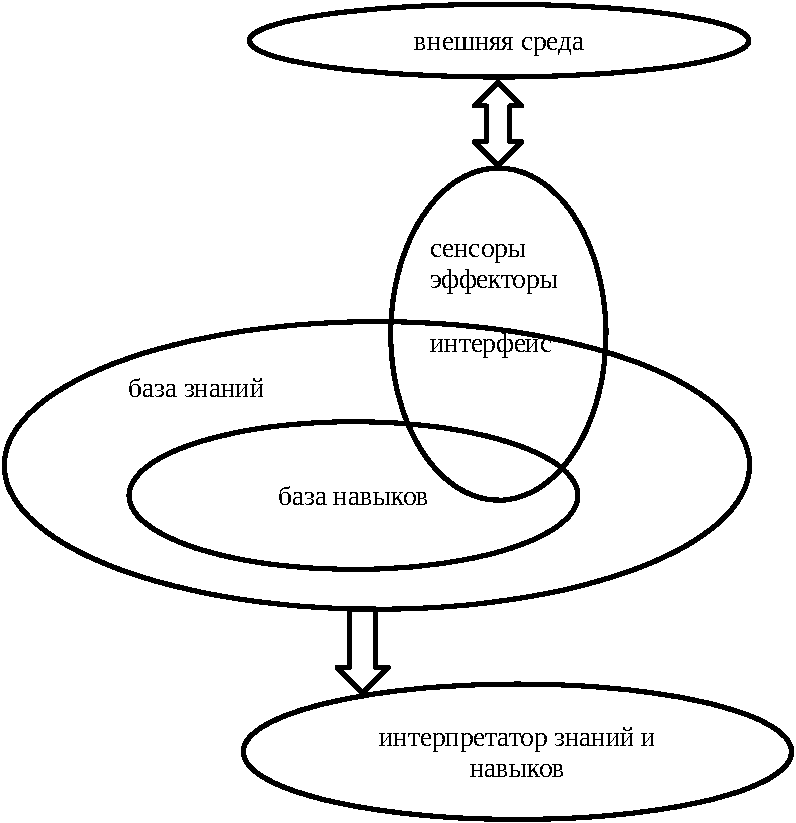
\includegraphics[width=0.5\linewidth]{figures/arch.pdf}\\}

\bigskip
\scnendstruct \scnendcurrentsectioncomment

\end{SCn}
\begin{SCn}

\scnsectionheader{Предметная область и онтология семантических моделей компьютерных систем}

\scnstartsubstruct

\scnheader{семантическая совместимость компьютерных систем}
\scnexplanation{Уровень совместимости \textit{компьютерных систем} определяется трудоемкостью реализации процедур интеграции (объединения, соединения знаний этих систем), а также трудоемкостью и глубиной интеграции входящих в эти системы \textit{решателей задач} (навыков и интерпретаторов этих навыков). Подчеркнем при этом, что интеграция интеграции рознь -- от эклектики до гибридности и синергетичности дистанция огромного размера.

Совместимые \textit{компьютерные системы} -- это компьютерные системы, для которых существует автоматически выполняемая процедура их интеграции, превращающая эти системы в единую \textbf{\textit{гибридную систему}}, в рамках которой каждая исходная компьютерная система в процессе своего функционирования может свободно использовать любые необходимые информационные ресурсы (знания и навыки), входящие в состав другой исходной компьютерной системы.

Целостную \textit{компьютерную систему} можно рассматривать как решатель задач, интегрировавший несколько моделей решения задач и обладающий средствами взаимодействия с внешней для себя средой (с другими компьютерными системами, с пользователями).

Таким образом, для того, чтобы повысить уровень совместимости \textit{компьютерных систем}, необходимо преобразовать их к виду \textit{многоагентных систем}, работающих над общей семантической памятью, в которой информация представлена семантическими сетями. Такие \textit{компьютерные системы} не всегда целесообразно непосредственно объединять (интегрировать) в более крупные \textit{компьютерные системы}. Иногда целесообразнее их объединять в \textit{коллективы взаимодействующих компьютерных систем}. Но при создании таких коллективов компьютерных систем унификация и совместимость таких систем также очень важны, т.к. существенно упрощают обеспечение высокого уровня их взаимопонимания. Так, например, противоречия между компьютерными системами, входящими в коллектив, можно обнаруживать путем анализа на непротиворечивость \textbf{\textit{виртуальной объединенной базы знаний}} этого коллектива. Более того, непротиворечивость указанной виртуальной базы знаний можно считать одним из критериев семантической совместимости систем, входящих в соответствующий коллектив.}

\scnheader{семантическая компьютерная система}
\scnexplanation{Предлагаемое нами устранение проблем современных информационных технологий путем перехода к \textit{смысловому представлению информации} в памяти компьютерных систем фактически преобразует современные компьютерные системы (в том числе и современные интеллектуальные системы) в \textit{\textbf{семантические компьютерные системы}}, которые, следовательно, являются не альтернативной ветвью развития \textit{компьютерных систем}, а естественным этапом их эволюции, направленным на обеспечение высокого уровня их обучаемости и, в первую очередь, \textbf{совместимости}.

Архитектура \textit{семантических компьютерных систем} (см. \textit{Рис. Архитектура семантических компьютерных систем}) практически совпадает с архитектурой интеллектуальных компьютерных систем, основанных на знаниях. Отличие здесь заключаются в том, что в \textit{семантических компьютерных системах}:
\begin{scnitemize}
    \item база знаний имеет смысловое представление;
    \item интерпретатор знаний и навыков представляет собой коллектив \textit{агентов}, осуществляющих обработку \textit{базы знаний}.
\end{scnitemize}

Как следствие этого, \textit{семантические компьютерные системы} обладают высоким уровнем обучаемости, т.е. способностью быстро приобретать новые и совершенствовать уже приобретенные знания и навыки и при этом не иметь никаких ограничений на вид приобретаемых и совершенствуемых ею знаний и навыков, а также на их совместное использование.

Более того, при согласовании соответствующих стандартов, а также при перманентном совершенствовании этих стандартов и при грамотной их поддержке в условиях интенсивной эволюции как самих стандартов, так и \textit{семантических компьютерных систем} (речь идет о постоянной поддержке соответствия между текущим состоянием компьютерных систем и текущим состоянием эволюционируемых стандартов), \textit{семантические компьютерные системы} и их компоненты обладают весьма высокой степенью совместимости.

Это, в свою очередь, практически исключает дублирование инженерных решений и дает возможность существенно ускорить разработку \textit{семантических компьютерных систем} с помощью постоянно расширяемой библиотеки многократно используемых и совместимых между собой компонентов. 

Основным лейтмотивом перехода от современных компьютерных систем (в том числе интеллектуальных) к семантическим компьютерным системам, т.е. компьютерным системам, основанным на смысловом представлении всей информации, хранимой в ее памяти, является создание \textit{\textbf{общей семантической теории компьютерных систем}}, включающей в себя:
\begin{scnitemize}
    \item cемантическую теорию знаний и баз знаний;
    \item семантическую теорию задач и моделей их решения;
    \item cемантическую теорию взаимодействия информационных процессов;
    \item cемантическую теорию пользовательских и, в том числе, естественно языковых интерфейсов;
    \item cемантическую теорию невербальных сенсорно-эффекторных интерфейсов;
    \item теорию универсальных интерпретаторов семантических моделей компьютерных систем и, в частности, теорию семантических компьютеров.
\end{scnitemize}

Эпицентром следующего этапа развития информационных технологий является решение проблемы обеспечения \textbf{семантической совместимости} \textit{компьютерных систем} и их компонентов. Для решения этой проблемы необходим
\begin{scnitemize}
    \item переход от традиционных компьютерных систем и от современных интеллектуальных систем к \textit{семантическим компьютерным системам};
    \item разработка \textit{стандарта семантических компьютерных систем}.
\end{scnitemize}    
    
Очевидно, что \textit{семантические компьютерные системы} являются компьютерными системами нового поколения, устраняющие многие недостатки современных компьютерных систем. Но для массовой разработки таких систем необходима соответствующая технология, которая должна включать в себя  

\begin{scnitemize}        
    \item теорию \textit{семантических компьютерных систем} и комплекс всех стандартов, обеспечивающих совместимость разрабатываемых систем;
    \item методы и средства проектирования \textit{семантических компьютерных систем};
    \item методы и средства перманентного совершенствования самой технологии.
\end{scnitemize}
}

\scnheader{Рис. Архитектура семантических компьютерных систем}
\scneqfile{\\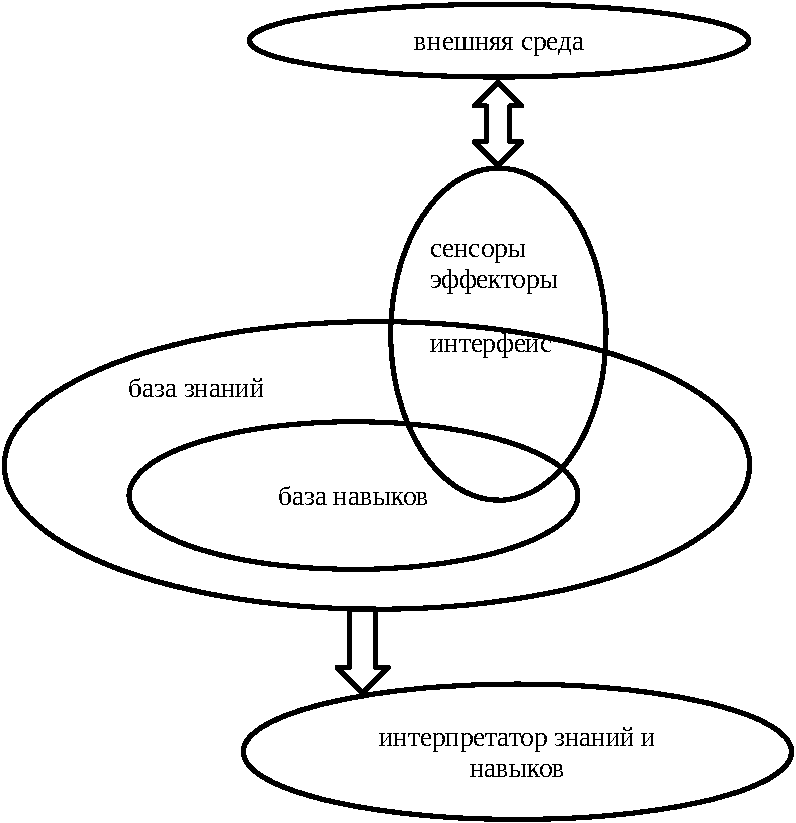
\includegraphics[width=0.5\linewidth]{figures/arch.pdf}\\}

\scnendstruct

\end{SCn}

\scsection{Предметная область и онтология смыслового представления информации}
\label{sd_sem_inf_rep}
\begin{SCn}

\scnsectionheader{\currentname}

\scnstartsubstruct

\scnrelto{частная предметная область и онтология}{Предметная область и онтология информационных конструкций}

\scnsdmainclasssingle{смысловое представление информации}

\scnsdclass{семантическая сеть\\
	\scnaddlevel{1}
	\scnsubdividing{нерафинированная семантическая сеть;рафинированная семантическая сеть}
	\scnsubdividing{абстрактная семантическая сеть\\
		\scnaddlevel{1}
		\scnidtf{семантическая сеть, абстрагирующаяся от того, как физически представлены ее элементарные (атомарные) фрагменты, а также связи инцидентности между этими фрагментами}
		\scnaddlevel{-1}
	;графически представленная семантическая сеть\\
		\scnaddlevel{1}
		\scnidtf{нарисованная семантическая сеть}
		\scnaddlevel{-1}
	;семантическая сеть, хранимая в графодинамической памяти\\
		\scnaddlevel{1}
		\scnrelboth{следует отличать}{представление семантической сети в адресной памяти}
			\scnaddlevel{1}
			\scnnotsubset{семантическая сеть}
			\scnidtf{представление семантической сети в виде линейной информационной конструкции, которая хранится в адресной памяти и которая, строго говоря, уже не является семантической сетью, но является информационной конструкцией, семантически эквивалентной соответствующей (представляемой) семантической сети}			
			\scnaddlevel{-1}
		\scnaddlevel{-1}}
	\scnaddlevel{-1}
;язык семантических сетей\\
	\scnaddlevel{1}
	\scnidtf{язык, все тексты которого являются семантическими сетями}
	\scnsubdividing{специализированный язык семантических сетей;универсальный язык семантических сетей}
	\scnsuperset{язык рафинированных семантических сетей}
	\scnaddlevel{-1}}

\scnrelfromvector{рассматриваемые вопросы}{
\scnfileitem{Что такое семантические сети и в чем их принципиальное отличие от других вариантов представления информации}
;\scnfileitem{До какой степени можно минимизировать алфавит элементов семантических сетей}
;\scnfileitem{Можно ли все описываемые связи свести к бинарным связям и почему это целесообразно}
;\scnfileitem{Можно ли разработать \uline{универсальный} язык семантических сетей}
;\scnfileitem{До какой степени можно упростить синтаксические структуры семантических сетей до, условно говоря, рафинированного вида}
;\scnfileitem{Какими достоинствами обладает семантические сети}}

\scnrelfromlist{ссылка}{Понятие Технологии OSTIS\\
	\scnaddlevel{1}
	\scnsourcecommentpar{Сегмент 3 Раздела 0.2}
	\scntext{аннотация}{В данном сегменте \textit{Документации Технологии OSTIS} рассматриваются принципы, лежащие в основе \textit{Технологии OSTIS}, основным из которых является ориентация на использование \textit{\uline{универсального} языка рафинированных семантических сетей} в качестве внутреннего языка \textit{интеллектуальных компьютерных систем}}
	\scnaddlevel{-1}
;Описание внутреннего языка ostis-систем\\
	\scnaddlevel{1}
	\scnsourcecommentpar{Раздел 0.3.1}	
	\scntext{аннотация}{В данном разделе \textit{Документации Технологии OSTIS} рассматриваются принципы, лежащие в основе \textit{универсального языка рафинированных семантических сетей}, используемого в качестве внутреннего языка \textit{ostis-систем} -- \textit{интеллектуальных компьютерных систем} следующего поколения}
	\scnaddlevel{-1}
;Описание языка графического представления знаний ostis-систем\\
	\scnaddlevel{1}
	\scnsourcecommentpar{Раздел 0.3.3}
	\scntext{аннотация}{В данном разделе \textit{Документации Технологии OSTIS} рассматриваются принципы, лежащие в основе универсального языка графически представленных семантических сетей, используемого в \textit{пользовательском интерфейсе ostis-систем}}
	\scnaddlevel{-1}
;Бирюков Б.В. ТеориСГФ-1960ст;Гладун В.П.;Скороходько;Мартынов;Шенк;Мельчук-Жолковский Смысл-Текст;Кузнецов Игорь}
	
\scnauthorcomment{Дооформить библиографию}	

\bigskip
\scnfragmentcaption

\scnheader{знак}
\scnidtf{фрагмент информационной конструкции, обладающий свойством, \uline{обозначать} некоторую сущность (объект), которая наряду с другими сущностями описывается указанной информационной конструкцией}
\scnnote{\uline{Форма} представления знаков в известной степени условна и является результатом соглашения между носителями соответствующего языка. Знак может быть, например, представлен:
	\begin{scnitemize}
	\item  в виде фрагмента речевого сообщения (последовательностью фонем);
	\item в виде строки символов (последовательности букв) в заданном алфавите;
	\item в виде иероглифа, пиктограммы;
	\item в виде жеста.
	\end{scnitemize}}
\scniselementrole{ключевой знак}{Предметная область и онтология информационных конструкций}
	\scnaddlevel{1}
	\scnsourcecommentpar{Раздел 2.1.2.0}
	\scnhaselement{раздел Базы знаний IMS.ostis}
	\scnaddlevel{-1}
\scntext{характеристика элементов данного множества}{Знаки, используемые в различных языках, характеризуются:
	\begin{scnitemize}
	\item синтаксической структурой, по совпадению (изоморфизму) которых для разных знаокв предполагается их синонимия;
	\item денотационной семантикой, т.е. той сущностью, которая обозначается соответствующим знаком;
	\item типом (классом) обозначаемой сущности, которая может быть:
	 	\begin{scnitemizeii}
		\item материальным(физическим) элементом (точкой) абстрактного пространства, множеством, которое может быть:
			\begin{scnitemizeiii}
			\item связью;
			\item классом;
			\item структурой;
			\end{scnitemizeiii}
		\item реальной и вымышленной сущностью;
		\item константной (конкретной) и переменной (произвольной) сущностью;
		\item постоянно существующей и временно существующей сущностью (прошлой, настоящей, будущей);		
		\end{scnitemizeii}
	\item множеством тех связей, которые связывают сущность, обозначаемую данным знаком с другими сущностями, а также, если данный знак обозначает некоторую связь, множеством сущностей, которые связаны этой связью, т.е. сущностей, являющихся компонентом этой связи;
	\item текущим статусом самого знака в памяти кибернетической системы, который может быть:
		\begin{scnitemizeii}
			\item логически удаленным знаком;
			\item настоящим знаком;
			\item предлагаемым (возможно, будущим) знаком.
		\end{scnitemizeii}
	\end{scnitemize}}
	
\scnheader{денотат*}
\scnidtf{денотат заданного знака*}
\scnidtf{объект, обозначаемый заданным знаком*}
\scnidtf{денотационная семантика заданного знака*}
\scnidtf{смысл заданного знака*}
\scnidtf{Бинарное ориентированное отношение, каждая пара которого связывает:
	\begin{scnitemize}
			\item некоторый знак, представленный в той или иной форме в тексте исследуемого языка;
			\item \uline{со знаком} той сущности, которая обозначается указанным выше знаком в рамках используемого метаязыка.
		\end{scnitemize}}
\scnnote{Данное отношение используется, когда с помощью одного языка необходимо описать денотационную семантику другого языка. Фактически речь идет о переводе заданного знака, входящего в состав некоторого рассматриваемого текста, принадлежащего некоторому исследуемому языку (языку-объекту), на некоторый метаязык (в нашем случае на SC-код), денотационная семантика которого нам считается априори известной. Указанный перевод есть связь заданного знака с синонимичным ему знаком, входящим в состав текста, принадлежащего указанному метаязыку.}
\scnrelboth{обратное отношение}{внешний sc-идентификатор*}
\scnaddlevel{1}
\scnidtf{быть знаком, обозначающим заданную сущность*}
\scnaddlevel{-1}
\scniselementlist{ключевой знак}{Описание внешних идентификаторов знаков, входящих в тексты внутреннего языка ostis-систем\\
	\scnaddlevel{1}
	\scnsourcecommentpar{Раздел 0.3.2}
	\scniselement{раздел Базы знаний IMS.ostis}
	\scnaddlevel{-1}
;Предметная область и онтология знаков, входящих в тексты внутреннего языка ostis-систем\\
	\scnaddlevel{1}
	\scnsourcecommentpar{Раздел 2.1.1.2}	
	\scniselement{раздел Базы знаний IMS.ostis}
	\scnaddlevel{-1}}
	
\scnheader{информационная конструкция}
\scnidtf{информация}
\scnnote{В общем случае информационная конструкция представляет собой сложную иерархическую структуру, каждому уровню иерархии которой соответствует определенный класс информационных конструкций.}
\scnsuperset{синтаксически элементарный фрагмент информационной конструкции}
	\scnaddlevel{1}
	\scnidtf{атомарный фрагмент информационной конструкции}
	\scnidtf{элемент информационной конструкции}
	\scnnote{Примерами таких элементарных фрагментов информационных конструкций являются буквы}
	\scnsuperset{буква}
	\scnaddlevel{-1}
\scnsuperset{простой знак}
	\scnaddlevel{1}
	\scnidtf{семантически элементарный фрагмент информационной конструкции}
	\scnsubset{знак}
	\scnaddlevel{-1}
\scnsuperset{выражение}
\scnaddlevel{1}
	\scnidtf{сложный (непростой) знак}
	\scnidtf{знак, являющийся одновременно некоторым знанием обозначаемой сущности (спецификацией этой сущности)}
	\scnidtf{знак, построенный как выражение вида "тот, который..."{}}
	\scnidtf{знак, в состав которого входят другие знаки}
	\scnsubset{знак}
	\scnaddlevel{-1}
\scnsuperset{простой текст}
	\scnaddlevel{1}
	\scnidtf{минимальная синтаксически целостная и корректная (правильная) информационная конструкция, включающая в себя:
	\begin{scnitemize}
	\item знак некоторой описываемой связи;
	\item минимальную спецификацию указанного знака связи (указание отношения, которому это связь принадлежит);
	\item указание \uline{всех} компонентов описываемой связи (знаков всех сущностей, связываемых этой связью, и/или всех знаков, связываемых этой связью -- описываемая связь может связывать не только "внешние"{} описываемые сущности, но и сами знаки);
	\item если описываемая связь не является бинарной, то связи с её компонентами могут потребовать явного представления знаков этих связей с дополнительным указанием роли этих компонентов.
	\end{scnitemize}}
	\scnsubset{текст}
	\scnaddlevel{-1}
\scnsuperset{сложный текст}
	\scnaddlevel{1}
	\scnidtf{информационная конструкция, являющаяся результатом соединения нескольких простых текстов}
	\scnsubset{текст}
	\scnaddlevel{-1}
\scnsuperset{простое знание}
	\scnaddlevel{1}
	\scnidtf{минимальная семантические целостная информационная конструкция}
	\scnidtf{знание, в состав которого не входят другие знания}
	\scnsubset{знание}
	\scnaddlevel{-1}	
\scnsuperset{сложное знание}
	\scnaddlevel{1}
	\scnidtf{информационная конструкция, являющаяся результатом соединения нескольких простых знаний}
	\scnidtf{знание, в состав которого не входят другие знания}
	\scnsubset{знание}
	\scnaddlevel{-1}	
\scniselementrole{ключевой знак}{Предметная область и онтология информационных конструкций}
\scnaddlevel{1}
	\scnsourcecommentpar{Раздел 2.1.2.0}
\scnaddlevel{-1}

\bigskip
\scnfragmentcaption

\scnheader{смысловое представление информации}
\scnidtf{смысловая форма представления информации}
\scnidtf{смысловое представление информационной конструкции}
\scnidtf{знаковая конструкция (текст), представленная в смысловой форме}
\scnidtf{смысловое представление информационной конструкции}
\scnidtftext{часто используемый sc-идентификатор}{смысл}
\scnidtf{смысловое представление}
\scnidtf{семантическое представление информации}

\scntext{основной принцип}{Как можно меньше лишнего, не имеющего отношения к смыслу представляемой информации.}
\scnidtf{такое представление информационной конструкции, которое существенно прощает соответствие между структурой самой этой информационной конструкции и описываемой (отображаемой) ею конфигурацией связей между рассматриваемыми (исследуемыми) сущностями}
\scnidtf{смысловое представление знаковой конструкции}
\scnidtf{абстрактная знаковая конструкция, являющаяся \uline{инвариантом} соответствующего максимального класса семантически эквивалентных знаковых конструкций}
\scnidtf{смысл информационной конструкции}
\scnidtf{денотационная семантика информационной конструкции}
\scnidtf{смысловое представление информационной конструкции}


\scnnote{Суть (смысл, денотационная семантика) любой информационной конструкции (информационной модели) сводится к описанию системы (конфигурации) связей между списываемыми (рассматриваемыми) сущностями. Важно, чтобы эта суть не была \uline{закамуфлирована} различными "синтаксическими"{} деталями, не имеющими никакого отношения к указанному смыслу (синтаксическая структура знаков, многократное повторение одного и того же знака, синонимия, омонимия, местоимения, предлоги, знаки препинания, разделители, ограничители, падежи и т.п.) а обусловленными \uline{формой} представления информационных конструкций, например, их линейностью.}


\scnexplanation{Смысловое представление любой информации в конечном счете сводится:
	\scnaddlevel{1}
	\begin{scnitemize}
		\item{к перечню знаков конкретных описываемых сущностей - как первичных сущностей, так и вторичных сущностей, которые сами являются информационными конструкциями (фрагментами данной конструкции)};
		\item{к явному описанию связи между знаками вторичных сущностей и самими этими сущностями (т.е. фрагментами информационной конструкции)};
		\item{к описанию других связей между описываемыми сущностями}
	\end{scnitemize}
}
\scnaddlevel{-1}

\scnauthorcomment{Дооформить ссылки}

\scnexplanation{Формализация смысла представляемой информации, т.е. строгое уточнение того, что такое \textit{смысловое представление информации}, является объективной основой для \uline{унификации} представления информации в \textit{памяти компьютерных систем} и \uline{ключом} к решению многих проблем семантической совместимости и эволюции компьютерных систем и технологий.

Согласно \textit{Мартынову В. В.} ~\scncite{Martynov}, <<фактически всякая мыслительная деятельность человека (не только научная), как полагают многие ученые, использует \uline{внутренний семантический код}, на который переводят с естественного языка и с которого переводят на естественный язык. Поразительная способность человека к идентификации огромного множества структурно различных фраз с одинаковым \textit{смыслом} и способность \uline{запомнить смысл вне этих фраз} убеждает нас в этом.>>

Приведем также слова \textit{Мельчука И. А.}~\scncite{MelchukST}:

<<Идея была следующая -- язык надо описывать следующим образом: надо уметь записывать смыслы фраз. \uline{Не фразы, а их \textit{смыслы}}, что отдельно. Плюс построить систему, которая по смыслу строит фразу. Это та область или тот поворот исследований, при котором интуиция способного лингвиста работает лучше всего: как выразить на данном языке данный смысл. Это -- то, для чего лингвистов учат..

Лингвистический \textit{смысл} научного текста -- это совсем не то, что ты, читая его, из него извлекаешь. Это, очень грубо говоря, инвариант синонимических перифраз. Ты можешь один и тот же смысл выразить очень многими способами. Когда ты говоришь, то можешь сказать по-разному: ``Сейчас я налью тебе вина'', или: ``Дай, я тебе предложу вина'', или: ``Не выпить ли нам по бокалу?'', -- все это имеет один и тот же смысл. И вот можно придумать, как записывать этот \textit{смысл}. Именно его. Не фразу, а \textit{смысл}. И работать надо от этого \textit{смысла} к реальным фразам. Синтаксис там по дороге тоже нужен, но он нужен именно по дороге, он не может быть ни конечной целью, ни начальной точкой. Это -- промежуточное дело.>>~\scncite{Melchuk}.
}

\scnnote{Грамотная унификация (стандартизация) \textit{смыслового представления информации} не должна привести к ограничению творческой свободы авторов различного вида публикуемых научно-технических знаний (и, в том числе, разработчиков \textit{баз знаний}), не должна гарантировать \textit{семантическую совместимость} различных \textit{знаний}, представленных различными авторами (разумеется, при условии соблюдения соответствующих правил построения этих \textit{знаний}). При этом любые \textit{стандарты} (в том числе и принятые стандарты \textit{смыслового представления информации}) должны постоянно эволюционировать. Текущая версия любого стандарта должна быть не догмой, а точкой опоры для дальнейшего совершенствования этого стандарта.}

\scnsuperset{УСК}
\scnaddlevel{1}
\scnidtf{Универсальный Семантический Код}
\scnrelfrom{автор}{Мартынов В. В.}
\scnnote{Разработанный Мартыновым В. В. Универсальный Семантический Код стал важнейшим этапом создания универсальных формальных средств смыслового представления знаний. Основная методологическая идея \textit{Мартынова В. В.}, касающаяся построения \textit{языка смыслового представления знаний}, заключается в том, чтобы выделить смысловые "кирпичики"{}, имеющие достаточно общий характер, а многообразие конкретных смыслов конструировать комбинаторно за счёт различных комбинаций (конфигураций) из этих "кирпичей"{}. Это можно назвать принципом минимизации типов атомарных смысловых фрагментов.}

\scnauthorcomment{Дооформить библиографию}

\scnrelto{ключевой знак}{Книга УСК}


\scnheader{смысловое представление информации*}
\scnidtfexp{\textit{Бинарное ориентированное отношение}, каждая \textit{пара} которого связывает некоторую \textit{информационную конструкцию} со смысловым представлением этой \textit{информационной конструкции*}.}

\scnsubset{формализация*}

\bigskip
\scnfragmentcaption

\scnheader{формализация*}
\scniselementrole{ключевой знак}{Начало Предметной области и онтологии кибернетических систем}
\scnaddlevel{1}
\scnsourcecommentpar{Начало Раздела 1.1}
\scniselement{начало раздела Базы знаний IMS.ostis}
\scnaddlevel{-1}
\scniselement{бинарное ориентированное отношение}
\scnidtf{формализация информации*}
\scnidtf{пара, связывающая менее формализованное и более формализованное представление некоторой информации*}
\scnidtf{формализация информационной модели некоторой описываемой (моделируемой) системы взаимосвязанных сущностей*}
\scnidtf{Бинарное ориентированное отношение, каждая \textit{пара} которого, связывает два \textit{семантически эквивалентных} знания, второе из которых является более точным (более точно сформированным) знанием по сравнению с первым \textit{знанием}*.}
\scnexplanation{Повышение точности (строгости) формулировки знания -- минимизация (а в идеале -- исключение) \uline{неоднозначной} семантической интерпретации этой формулировки, т.е. несоответствия того, что хотел "сказать"{} автор формулировки, и того, как его поняли. Формализация знаний предполагает (1) точное (строгое) описание \textit{синтаксиса и денотационной семантики} того \textit{языка}, на котором формулируются \textit{знания} и (2) максимально возможное \uline{упрощение} синтаксических и семантических принципов, лежащих в основе указанного \textit{языка}. Очевидно, что \textit{естественные языки} указанным требованиям не удовлетворяют и, следовательно, не могут быть основой для точной формулировки \textit{научно-технических знаний} и, соответственно, для представления этих \textit{знаний} в \textit{памяти интеллектуальных компьютерных систем}. Очевидно также, что разработка \textit{\uline{универсального} языка} формального представления научно-технических знаний является \uline{основой} для глубокой конвергенции различных научно-технических дисциплин, для расширения областей применения современной математики и даже для появления новых разделов математики, которые, например, изучают общие свойства \textit{универсального смыслового пространства} и, в частности, свойство семантического расстояния(семантической близости) как между различными \textit{знаками}, так и между различными \textit{знаковыми конструкциями} (конфигурациями знаков).}
\scnaddlevel{1}
\scnnote{Слово "математика"{} означает "точное знание"{}.}
\scnaddlevel{1}
\scnrelto{цитата}{\textit{Арнольд В.И. Что TM--2012кн-c.4}}
\scnaddlevel{-2}
\scnauthorcomment{Дооформить}

\scnnote{Формализация информационной модели есть не что иное как "движение"{} в сторону семантического (смыслового) представления этой модель, т.е. переход к такому представлению этой модели, в котором мы избавляемся от всего, не имеющего отношения к сути моделируемой системы и касающегося только способа построения этой модели (т.е. её синтаксической структуры). }
\scnnote{Нет проблемы записать любое \textit{знание} в компьютерную \textit{память}. Для этого надо придумать соответствующий формат их кодирования. Но есть проблема представить это \textit{знание} так, чтобы с ним было легко работать, чтобы с использованием этого \textit{знания} можно было достаточно удобно (без лишних накладных расходов, обусловленных выбранным способом представления) решать самые различные информационные \textit{задачи} (задачи интеграции знаний, информационного поиска по базе знаний, верификации и оптимизации баз знаний, логического вывода, поиска способов решения задач, хранимых в базе знаний и т. д.).
Какими характеристиками должно обладать удобное представление знаний, удовлетворяющее указанным требованиям. Очевидно, что такое представление есть не что иное, как формальная (математическая) модель, семантически эквивалентная этим знаниям. Т.е. удобно представить знание -- это фактически построить соответствующую этому знанию \textit{математическую модель}.
Для интеллектуальных компьютерных систем важно не просто приобрести знания, но и представить их в такой форме, которая была бы удобна не только для человека (пользователя и разработчика), но и для различных компьютерных систем, т.е. не требовала бы переоформление (перезаписи) этих знаний для различных компьютерных систем. Очевидно, что такая форма записи (представления) знаний должна быть абсолютно не зависящий от различных компьютерных платформ.
Это и есть главная цель формализации знаний, обеспечивающей эффективную автоматизацию обработки этих знаний.}
\scnheader{формальное представление информации}\\
\scnsubset{информация}
\scnaddlevel{1}
\scnidtf{информационная конструкция}
\scnaddlevel{-1}
\scntext{вопрос}{Почему разработка и использование формальных моделей (математических моделей) представления \textit{информации} является важнейшим этапом развития любой научной и научно-технической дисциплины.
}\scnaddlevel{1}
\scnrelfromset{ответ}{\scnfileitem{Формализация любой \textit{предметной области} даёт возможность более конструктивно накапливать, интегрировать, понимать и систематизировать новые \textit{знания} об этой \textit{предметной области}};
\scnfileitem{Формализация \textit{предметной области} обеспечивает более строгую верификацию, обоснование (аргументацию, доказательство) и согласование различных точек зрения};
\scnfileitem{Формализация \textit{предметной области} создает условия для разработки строгих и легко воспроизводимых (реализуемых) \textit{методов} решения различных \textit{классов задач}}}
\scnaddlevel{1}
\scniselement{конъюнкция*}
\scnrelto{достоинства}{формальное представление информации}
\scnaddlevel{-2}
\scnidtf{формальное (формализованное) представление информационной конструкции}
\scnsubset{смысловое представления информации}
\scnnote{Высшим уровнем качества \textit{формального представления информации} является смысловое представление этой информации}
\scnidtf{формальная модель системы описываемых взаимосвязанных сущностей}
\scnidtf{математическая модель системы описываемых взаимосвязанных сущностей}
\scnidtf{формула}
\scnnote{Сам термин ``\textit{формальное представление информации}'' свидетельствует о том, что при таком представлении \textit{информации} сама \uline{форма} представляемой информационной конструкции (т.е. синтаксическая структура этой конструкции) имеет очевидную аналогию с описываемой конфигурацией связей между соответствующими соответствующими описываемыми \textit{сущностями}.
В предельном "идеальном"{} случае указанная аналогия между формой и смыслом информационной конструкции должна быть изоморфизмом.}
\scnnote{Формализация формализации рознь и, соответственно, степень приближения формы представления информации к "идеальному"{} смысловому представлению может быть различной. Разработка такого "идеального"{} \textit{языка смыслового представления информации} должна руководствоваться следующими основными критериями:
	\begin{scnitemize}		
		\item максимально возможное упрощения синтаксиса (как можно меньше синтаксических излишеств и синтаксического разнообразия).
		\item обеспечение \uline{универсальности} языка.
	\end{scnitemize}

Подчеркнем, что обеспечение универсальности \textit{языка смыслового представления информации} является весьма нетривиальной задачей, т.к. сложно одновременно достигнуть две противоречащие друг другу цели- обеспечить простоту синтаксиса языка и его неограниченную семантическую мощность. Косвенным подтверждением этого является большое количество созданных человечеством специализированных \textit{формальных языков}, \textit{языков смыслового представления информации} и даже \textit{языков семантических сетей}, что свидетельствует о востребованности \textit{смыслового представления информации}.}
\scnsubdividing{формальное представление информации, не являющееся смысловым
;смысловое представление информации, не являющееся семантической сетью
;нерафинированная семантическая сеть
\scnaddlevel{1}
\scnidtf{смысловое представления информации 2-го уровня}
\scnaddlevel{-1}
;рафинированная семантическая сеть
\scnaddlevel{1}
\scnidtf{смысловое представление информации 3-го уровня}
\scnaddlevel{-1}}

\bigskip
\scnfragmentcaption

\scnheader{смысловое представление информации, не являющееся семантической сетью}
\scnnote{Данному уровню смыслового представления информации соответствуют предлагаемые нами универсальные формальные языки SCs-код и SCn-код}

\scnsuperset{SCs-код}
\scnaddlevel{1}
\scniselement{универсальный формальный язык}
\scniselementrole{ключевой знак}{Описание языка линейного представления знаний ostis-систем}
\scnaddlevel{-1}
\scnsuperset{SCn-код}
\scnaddlevel{1}
\scniselement{универсальный формальный язык}
\scniselementrole{ключевой знак}{Описание языка структурированного представления знаний ostis-систем}
\scnaddlevel{-1}

\scnreltovector{принципы, лежащие в основе}{\scnfileitem{В состав \textit{смыслового представления информации, не являющегося семантической сетью} могут входить все уровни иерархии представления информационной конструкции --
\begin{scnitemize}
		\item синтаксически элементарные фрагменты информационной конструкции, из которых строятся простые знаки описываемых сущностей, а также разделители и ограничители;
		\item простые знаки;
		\item выражения;
		\item простые тексты;
		\item сложные тексты;
		\item простые знания;
		\item сложные знания.
\end{scnitemize}};
\scnfileitem{Множество всех описываемых сущностей, \uline{не являющихся связями}, разбивается на два подмножества:
\begin{scnitemize}
	\item каждой сущности, принадлежащей первому подмножеству, \uline{взаимно однозначно} соответствует множество \uline{синтаксически эквивалентных} (синтаксически одинаковых) \textit{простых знаков}, каждый из которых обозначает указанную сущность;
	\item каждой сущности, принадлежащей второму подмножеству, соответствует в общем случае \uline{семейство} множеств, кажо из которых является максимальным множеством синтаксически эквивалентных выражений, обозначающих указанную сущность.
\end{scnitemize}
}
\scnaddlevel{1}
\scntext{следовательно}{Здесь синонимия \textit{простых знаков}, имеющих \uline{разную} синтаксическую структуру, отсутствует, а вот синонимия \textit{выражений}, имеющих разную синтаксическую структуру, вполне возможна. Подчеркнем при этом, что в рамках \textit{смыслового представления информации, не являющегося семантической сетью}, \scnbigspace \textit{знаки} (как \textit{простые знаки}, так и \textit{выражения}), имеющие одинаковую синтаксическую структуру, считаются также и семантически эквивалентными, т.е. обозначающими одну и ту же сущность. Это означает отсутствие омонимии синтаксически эквивалентных знаков.}
\scntext{следовательно}{В рамках \textit{смыслового представления информации, не являющегося семантической сетью}, простые знаки, обозначающие \uline{разные} сущности, имеют легко устанавливаемое отличие своих синтаксических структур, а простые знаки, обозначающие одну и ту же сущность имеют легко устанавливаемое сходство своих синтаксических структур. Таким образом, в рамках \textit{смыслового представления информации, не являющегося семантической сетью}, \scnbigspace \uline{дублирование знаков}, т.е. многократное вхождение \textit{знаков} одной и той же сущности, \uline{допускается}.}
\scnaddlevel{-1};
\scnfileitem{Связи как вид описываемых сущностей имеют очень важные особенности:
\begin{scnitemize}
	\item каждой описываемой \textit{связи} \uline{однозначно}, а в подавляющем числе случаев и \uline{взаимно однозначно} соответствует \textit{простой текст}, являющийся контекстом (спецификацией) этой \textit{связи};
	\item весьма редки \textit{кратные связи}, т.е. \textit{свзяи}, принадлежащие одному и тому же \textit{отношению} и связывающие одинаковым образом одни и те же \textit{сущности};
	\item довольно редко \textit{связи} являются компонентами других \textit{связей}.
\end{scnitemize}}
\scnaddlevel{1}
\scntext{следовательно}{Для подавляющего числа описываемых \textit{связей} нет никакой необходимости вводить обозначающие их \textit{знаки}, если эти \textit{связи} описываются соответствующими \textit{простыми текстами}. Вместо таких \textit{знаков} можно ввести условные представления этих \textit{связей}, отражающие их вид и направленность. Такие условные представления (изображения) описываемых \textit{связей} можно считать \textit{знаками}, но \textit{знаками}, семантические свойства которых принципиально отличаются от тех \textit{знаков} описываемых \textit{сущностей}, которые мы рассматривали выше. Любые данного вида разные \textit{знаки} описываемых \textit{связей} даже, если, они являются \textit{синтаксически эквивалентными}, т.е. имеют одинаковую структуру, считаются \textit{знаками} \uline{разных} описываемых \textit{связей}. Синонимия таких \textit{знаков} принципиально возможна, но только в том случае, если \textit{простые тексты}, описывающие соответствующие \textit{связи}, будут полностью \uline{продублированы}.}
\scnaddlevel{-1};
\scnfileitem{Для описания связей между описываемыми сущностями в смысловом представлении информации нет необходимости использовать такие приемы естественных языков, как склонения, спряжения, семантическая значимость последовательности знаков.};
\scnfileitem{В случае, если с помощью \textit{простых текстов} необходимо описать контекст (спецификацию) нескольких \uline{кратных} \textit{связей}, все эти \textit{связи} необходимо обозначить \textit{знаками} первого типа -- знаками, \textit{синтаксическая структура} каждого из которых \uline{уникальна.}
Кроме этого, необходимо ввести знак, который обозначает \textit{связь инцидентности} между описываемой \textit{связью} и компонентом этой \textit{связи}, и который относится к числу \textit{знаков} второго типа -- \textit{знаков}, разные экземпляры (разные вхождения) которого считаются обозначениями \uline{разных} \textit{связей}};
\scnfileitem{Для явного указания синонимии двух разных \textit{знаков} первого типа, имеющих разную \textit{синтаксическую структуру}, вводится фиктивная \textit{связь равенства}, которая сама не является описываемой \textit{связью}, а только указывает факт синонимии двух \textit{знаков}, по крайней мере один из которых должен быть \textit{выражением}.};
\scnfileitem{Каждая описываемая \textit{сущность} должна быть специфицирована путем указания типа этой \textit{сущности}. Описываемая \textit{сущность} может быть:
\begin{scnitemize}
	\item \textit{материальной сущностью};
		  \newline
		  \textit{точкой абстрактного пространства};
		  \newline
		  \textit{множеством}:
		  \begin{scnitemizeii}
		  	\item \textit{связью};
		  	\item \textit{классом};
		  	\item \textit{структурой};
		  \end{scnitemizeii}
	\item \textit{реальной сущностью};
		  \newline
		  \textit{вымышленной сущностью};
	\item \textit{константой};
		  \newline
		  \textit{переменной};
	\item \textit{постоянной сущностью};
		  \newline
		  \textit{временной сущностью}:
		  \begin{scnitemizeii}
		  	\item \textit{прошлой сущностью};
		  	\item \textit{настоящей сущностью};
		  	\item \textit{будующей сущностью}.
		  \end{scnitemizeii}
\end{scnitemize}
Кроме того, сам \textit{знак} описываемой сущности может иметь следующий статус:
\begin{scnitemize}
	\item \textit{логически удаленный знак};
	\item \textit{настоящий знак};
	\item \textit{будущий знак}.
\end{scnitemize}};
\scnfileitem{Возможно дублирование информации, т.е. могут присутствовать семантически эквивалентные информационные конструкции, входящие в остав одной информационной конструкции (например, в состав информации, хранимой в памяти одной компьютерной системы). Но при этом есть принципиальная возможность обнаружить такое дублирование информации.}}

\bigskip
\scnfragmentcaption

\scnheader{графовая структура}

\scnidtfdef{абстрактная (математическая) структура, которая задается:
\begin{scnitemize}
	\item множеством ее элементов:
		\begin{scnitemizeii}
		 \item множеством ее вершин (узлов);
		 \item множеством ее связок:
		 \begin{scnitemizeiii}
		 \item множеством ее ребер (неориентированных пар 		элементов графовой структуры);
		 \item множеством ее дуг (ориентированных пар элементов графовой структуры);
		 \item множеством ее гиперребер, каждое из которых является конечным множеством элементов графовой структуры, имеющим мощность больше двух
		 \end{scnitemizeiii}
		 \end{scnitemizeii}
	\item бинарным ориентированным отношением инцидентности, связывающим каждую связку графовой структуры с каждым компонентом (элементом) этой связки.
\end{scnitemize}}

\scnheader{следует отличать*}
\scnhaselementset{\scnfileitem{\textit{графовую структуру} как абстрактный математический объект, в рамках которого не уточняется то, как выглядят (представляются, изображаются) элементы графовой структуры и связи их инцидентности}
;\scnfileitem{представление (изображение) \textit{графовой структуры} -- ее рисунок, ее представление в компьютерной памяти в виде матрицы инцидентности, матрицы смежности, списковой структуры}}


\scnheader{графовая структура}
\scnidtftext{часто используемый sc-идентификатор}{дискретная информационная конструкция}
\scnnote{Поскольку любая \textit{графовая структура} является дискретной математической моделью, которая может описывать любое множество \textit{сущностей}, связанных между собой заданным множеством \textit{связей}, все \textit{графовые структуры} с полным основанием можно считать дискретными \textit{информационными конструкциями}. Более того, любая дискретная \textit{информационная конструкция} (в том числе, и обычная цепочка символов) с формальной точки зрения является \textit{графовой структурой}. Тот факт, что теория графов рассматривает "синтаксические"{} свойства \textit{графовых структур} с точностью до их изоморфизма, не лишает \textit{графовые структуры} соответствующих "семантических"{} свойств.}
\scnexplanation{С семантической точки зрения графовая структура -- это нелинейная (в общем случае) знаковая конструкция, в состав которой могут входить знаки \uline{любых} сущностей. При этом указанные знаки \uline{синтаксически} разбиваются на два класса --
	\begin{scnitemize}
		\item на \textit{знаки} сущностей, которые не являются \uline{связями} между сущностями -- в теории графов такие знаки называются узлами (вершинами);
		\item на знаки \uline{связей} между \textit{сущностями} -- к таким \textit{знакам} относятся ребра неориентированных графов, гиперребра гиперграфов, дуги ориентированных графов.
	\end{scnitemize}	
Кроме того, на множестве знаков \textit{сущностей}, входящих в состав \textit{графовой структуры}, задаются \textit{отношения инцидентности}, которые связывают \textit{знаки} связей, входящих  в состав \textit{графовой структуры}, со знаками тех \textit{сущностей} которые являются компонентами указанных \textit{связей}.


Теория графов рассматривает только "синтаксические"{} аспекты \textit{графовых структур}.
Семантика \textit{графовой структуры} задается \textit{онтологией}, специфицирующей систему понятий, экземплярами которых являются элементы этой графовой структуры, т.е. \textit{знаки}, входящие в состав этой \textit{графовой структуры}.}


\scnheader{семантическая сеть}
\scnidtf{\textit{графовая структура}, являющаяся \uline{формальным уточнением} одного из видов \textit{смыслового представления информации}}
\scnsubset{графовая структура}
\scnsubset{смысловое представление информации}
	\scnaddlevel{1}
	\scnsubset{знаковая структура}
	\scnaddlevel{-1}
\scnidtf{графовая структура, \uline{вершины} (узлы) которой трактуются как знаки некоторых описываемых сущностей, а \uline{связки} (ребра, дуги, гиперребра, гипердуги) которой трактуются как знаки связей между описываемыми сущностями и/или знаками этих сущностей} 
\scnidtf{\uline{абстрактная} графовая и в общем случае нелинейная знаковая конструкция (знаковая структура), являющаяся вариантом \uline{смыслового} представления соответствующей информации}
\scnidtfexp{информационная конструкция, в которой \uline{явно} выделены знаки \uline{всех} описываемых сущностей, а также знаки связей, которые также считаются описываемыми сущностями и которые связывают либо сами описываемые сущности, либо описываемые сущности со знаками других описываемых сущностей, лиюо знаки описываемых сущностей}
\scnnote{Теоретико-графовая трактовка (уточнение) \textit{смыслового представления информации} является вполне естественной, т.к. любая описываемая сущность может иметь неограниченное количество связей с другими описываемыми сущностями, и очень часто анализ свойств какой-либо описываемой сущности предполагает анализ всех представленных (описанных) связей этой сущности с различными другими сущностями. Более того, для любых описываемых сущностей существует связывающая их связь (все в Мире взаимосвязано). Вопрос в том, какая это связь и нужно ли ее описывать. Далеко не все то, что можно описывать, целесообразно описывать.}
\scnrelfromvector{общие предпосылки}{
\scnfileitem{Информация в знаковой конструкции содержится не в самих знаках, а в конфигурации связей между знаками, обозначающими описываемые сущности}
;\scnfileitem{Конфигурация связей между описываемыми сущностями \uline{в общем случае} \uline{не} являются линейной} 
;\scnfileitem{Идеальным \textit{смысловым представлением информации} следует считать такую знаковую конструкцию, синтаксическая конфигурация связей между знаками которой \uline{изоморфна} конфигурации связей между описываемыми сущностями}}
\scnnote{Понятие семантической сети является основным понятием для \textit{Технологии OSTIS}. Ранее семантические сети рассматривались не как основа технологии разработки интеллектуальных компьютерных систем, а как наглядная иллюстрация представления знаний, не имеющая практической перспективы из-за сложности реализации, не обладающая универсализмом.


Для нас семантические сети -- это
	\begin{scnitemize}
	\item формальный подход к построению знаковых конструкций:
	\item формальный подход, позволяющий создавать целое \uline{семейство} языков и в том числе языков \uline{универсальных}:
	\item основа организации памяти нового типа -- структурно перестраиваемой (реконфигурируемой) памяти, обработка информации в которой сводится к реконфигурации связей между ее элементами.
	\end{scnitemize}}

\scnrelfromlist{достоинства}{\scnfileitem{\textbf{Семантическая сеть} наряду с системами правил является весьма распространенным способом представления знаний в интеллектуальных системах. Особое значение этот способ представления знаний приобретает в связи с развитием сети интернет. Кроме ряда особенностей, позволяющих применять семантические сети в тех случаях, когда системы правил не применимы, \textbf{семантические сети} обладают следующим важным свойством: они дают возможность \textbf{соединения в одном представлении синтаксиса и семантики} или \uline{синтаксического и семантического аспектов описаний} знаний предметной области. Происходит это благодаря тому, что в семантических сетях наряду с переменными для обозначения тех или иных объектов (элементов множеств, некоторых конструкций из них) присутствуют и сами эти элементы и конструкции; присутствуют и связи, сопоставляющие тем или иным переменным множества допустимых интерпретаций. Эти обстоятельства позволяют во многих случаях резко \textbf{уменьшить реальную вычислительную сложность решаемых задач}.
\newline
Помимо изобразительных возможностей, \textbf{семантические сети обладают более серьезными достоинствами}. То обстоятельство, что \textbf{вся информация об индивиде представлена в единственном месте} -- в одной вершине -- означает, что вся эта информация непосредственно доступна в этой вершине, что, в свою очередь, \textbf{сокращает время поиска}, в частности, при выполнении унификации и подставновки в задачах логического вывода.
Существует еще одна, более \textbf{тонкая особенность} расширенных семантических сетей -- они позволяют \textit{интегрировать в одном представлении \textbf{синтаксис и семантику}} (т.е. интерпретацию) клаузальных форм. Это позволяет в процессе вывода обеспечивать взаимодействие синтаксических и семантических, теоретико-модельных подходов, что, в свою очередь, также является фактором, зачастую делаютщим вывод практически более эффективным}\\
	\scnaddlevel{1}
	\scnrelto{цитата}{Осипов Г.С.-Метод ИИ-2015кн,с.43-54}
	\scnaddlevel{1}
	\scnrelto{часть}{Осипов Г.С.-Метод ИИ-2015кн}
	\scnaddlevel{-2}
;\scnfileitem{Все связи между \textit{знаками}, входящими в состав \textit{семантической сети} представляются с помощью специальных связующих элементов \textit{семантической сети} (дуг, ребер) и, следовательно, для описания указанных связей в \textit{семантической сети} нет необходимости использовать такие средства, как предлоги, союзы, падежи, склонения, спряжения, различные разделители и ограничители, что существенно упрощает обработку \textit{знаний}.}
;\scnfileitem{Соединение синтаксических и семантических аспектов в \textit{семантической сети} проявляется в том, что дуга или ребро, "синтаксически"{} соединяющая элементы \textit{семантической сети} описывает наличие соответствующей \textit{связи} между \textit{сущностями}, обозначаемыми указанными элементами \textit{семантической сети}.}}

\scnauthorcomment{Дооформить ссылки}


\bigskip
\scnfragmentcaption

\scnheader{нерафинированная семантическая сеть}
\scnnote{Переход от смыслового представления информации, не являющегося семантической сетью, к нерафинированным семантическим сетям представляет собой переход к информационным конструкциям, имеющим более простую синтаксическую структуру и денотационную семантику.\\
\newline
К нерафинированным семантическим сетям можно отнести тексты предлагаемого нами универсального формального SCg-кода, а также используемые в Semantic Web rdf-графы}

\scnsuperset{SCg-код}
\scnaddlevel{1}
\scnhaselement{универсальный формальный язык}
\scnhaselementrole{ключевой знак}{Описание языка графического представления знаний ostis-систем}
\scnaddlevel{-1}
\scnsuperset{rdf-граф}

\scnreltovector{принципы, лежащие в основе}{\scnfileitem{Поскольку в \textit{информационной конструкции} информация содержится не в самих \textit{знаках} (если не считать \textit{знаки}, являющиеся \textit{выражениями}), а в конфигурации связей между \textit{знаками}, очень важно \uline{явно} формально представить саму эту конфигурацию \textit{знаков}. И как нельзя лучше для этого подходит понятие \textit{графовой структуры} и, соответственно, понятие \textit{семантической сети}.\\
Что касается \textit{выражений}, то каждое из них легко трансформируется в \textit{семантически эквивалентную} информационную конструкцию, не являющиюся \textit{выражением}. Заметим, что \textit{выражения} используются исключительно для минимизации числа вводимых \textit{знаков} (имен) с уникальной синтаксической структурой.}
;\scnfileitem{\uline{Все} элементы, входящие в состав нерафинированной семантической сети и представленные узлами, ребрами или дугами, являются \textit{знаками}, обозначающими соответствующие описываемые \textit{сущности}, причём \textit{знаками} второго типа, которые, обозначая соответствующую \textit{сущность}, входят в \textit{информационную конструкцию} \uline{однократно} (отсутствует многократное вхождение \textit{знаков}, обозначающих одну и ту же \textit{сущность}). Также \textit{знаки} могут иметь синтаксическую структуру, которая не является уникальной для обозначаемой \textit{сущности}, а отражает только принадлежность этой сущности к соответствующих классам.
Таким образом, в \textit{нерафинированной семантической сети} в отличие от \textit{смыслового представления информации не являющегося семантической сетью}, доминируют не \textit{знаки} первого типа, а \textit{знаки} второго типа, которыми в \textit{нерафинированной семантической сети} представлены (обозначены) \uline{все} описываемые \textit{сущности}, а в \textit{смысловом представлении информации, не являющемся семанитеской сетью}, представлены \uline{только} \textit{бинарные связи} \uline{и то не все}.}
;\scnfileitem{\uline{Все} ребра \textit{нерафинированной семантической сети} являются знаками \textit{бинарных неориентированных связей} и формально трактуются как знаки \textit{двухмощных множеств}, каждым \textit{элементом} которых являются либо знак \textit{сущности}, соединяемой указанной \textit{бинарной связью}, либо \textit{знак}, который сам является \textit{сущностью}, соединяемой этой \textit{бинарной связью}. Более того, \uline{все} \textit{двухмощные множества}, не являющиеся \textit{кортежами} (ориентированными парами) в \textit{нерафинированной семантической сети} обозначаются \textit{ребрами} этой сети.}
;\scnfileitem{\uline{Все} дуги \textit{нерафинированной семантической сети} являются знаками \textit{бинарных ориентированных связей} и формально трактуются как знаки \textit{двухмощных кортежей} (ориентированных пар), каждым \textit{элементом} которых является либо знак \textit{сущности}, соединяемой указанной \textit{бинарной связи}, либо \textit{знак}, который сам является \textit{сущностью}, соединяемой этой \textit{бинарной связью}. Более того, \uline{все} \textit{ориентированные пары} в \textit{нерафинированной семантической сети} обозначаются \textit{дугами} этой сети.}
;\scnfileitem{\uline{Каждая} небинарная связь, описываемая в нерафинированной семантической сети, трактуется как множество, мощность которого не равна двум и обозначается соответствующим узлом этой сети, который соединяется дугами, принадлежащими отношению принадлежности со всеми знаками, которые либо обозначаются сущности, связывающие рассматриваемой небинарной связью, либо сами являются такими сущностями. Для описания ориентированных небинарных связей (в частности, небинарных кортежей) выделяется несколько подмножеств отношения принадлежности, соответствующих различным ролям элементов (компонентов) ориентированных небинарных связей.}
;\scnfileitem{В рамках нерафинированной семантической сети \uline{все} рассматриваемые связи между описываемыми сущностями представляются \uline{явно} в виде знаков, обозначающих эти связи.}
;\scnfileitem{В рамках нерафинированной семантической сети не используются такие средства, как разделители, ограничители и др.}
;\scnfileitem{Узлами \textit{нерафинированной семантической сети}, которые обозначают различного вида \uline{ключевые} описываемые \textit{сущности} (прежде всего, различные \textit{понятия}) приписываются уникальные \textit{знаки} (имена) этих \textit{ключевых сущностей}. Очевидно, что каждый такой \textit{узел} и приписываемое ему \textit{имя} -- это \textit{синонимичные знаки}, обозначающие одну и ту же \textit{сущность}, но являющиеся \textit{знаками} двух разных типов -- (1) \textit{знаком}, который \uline{однократно} представлен в рамках \textit{информационной конструкции}; (2) \textit{знаком}, синтаксическая структура которого \uline{взаимно однозначно} соответствует обозначаемой им \textit{сущности}.}
;\scnfileitem{Большинству узлов, обозначающих небинарные связи, большинству ребер и дуг, а также некоторым другим узлам нерафинированной семантической сети могут быть приписаны уникальные знаки (в частности, имена) понятий (чаще всего, отношений), которым принадлежат указанные узлы, ребра и дуги.}}

\bigskip
\scnfragmentcaption

\scnheader{рафинированная семантическая сеть}
\scntext{основной принцип}{Абсолютно ничего лишнего, не имеющего отношения к смыслу представляемой информации}
\scnidtf{\uline{предельно} компактная (сжатая) смысловая информационная модель соответствующей системы рассматриваемых (описываемых, исследуемых, моделируемых) сущностей}
\scnnote{Указанная система рассматриваемых сущностей представляет собой конфигурацию связей между этими сущностями. Подчеркнем при этом, что указанные связи между рассматриваемыми сущностями также входят в число рассматриваемых сущностей.}

\scnidtf{\textit{информационная конструкция}, являющаяся результатом максимально возможного упрощения ее \textit{синтаксической структуры} при обеспечении представления \uline{любой} \textit{информации}, что приводит к фактическому слиянию синтаксических и семантических аспектов представления \textit{информации}}
\scnidtf{\textit{семантическая сеть} "внутреннего"\ потребления, используемая для \textit{смыслового представления информации} в памяти \textit{компьютерных систем}}
\scnidtf{уточнение принципов \textit{смыслового представления информации}, которое основано, \uline{во-первых}, на четком противопоставлении \textit{внутреннего языка компьютерной системы}, используемого для хранения информации в памяти компьютера, и \textit{внешних языков компьютерной системы}, используемых для общения (обмена сообщений) \textit{компьютерной системы} с пользователями и другими \textit{компьютерными системами} (рафинированная семантическая сеть используется исключительно для \textit{внутреннего представления информации} в памяти \textit{компьютерной системы}), и, \uline{во-вторых} на максимально возможном упрощении \textit{синтаксиса внутреннего языка компьютерной системы} при обеспечении \uline{универсальности} путем исключения из такого внутреннего универсального языка средств, обеспечивающих коммуникационную функцию \textit{языка} (т.е. обмен сообщениями). 
\newline
Так, например, для \textit{внутреннего языка компьютерной системы} излишними являются такие коммуникационные средства \textit{языка}, как союзы, предлоги, разделители, ограничители, склонения, спряжения и другие.
\newline
\textit{Внешние языки компьютерной системы} могут быть как близки ее внутреннему языку, так и весьма далеки от него (как, например, \textit{естественные языки}).}
\scnidtf{\uline{абстрактная} знаковая конструкция, принадлежащая \uline{универсальному} внутреннему языку компьютерных систем и являющаяся \uline{инвариантом} соответствующего максимального множества семантически эквивалентных знаковых конструкций (текстов), принадлежащих самым различным языкам}

\scnrelfromvector{принципы лежащие в основе}{\scnfileitem{Каждый фрагмент \textit{рафинированной семантической сети} является либо \textit{знаком} (элементарным фрагментом, представленным либо \textit{узлом}, либо \textit{ребром}, либо \textit{дугой}), либо множеством \textit{знаков}, связанных между собой отношением \textit{инцидентности} элементов \textit{рафинированной семантической сети}. Указанное отношение \textit{инцидентности} является \textit{бинарным ориентированным отношением}, связывающим \textit{знаки} описываемых \textit{связей} (которые представляются \textit{ребрами}, \textit{дугами} и \textit{узлами}, если описываемая связь является небинарной) со \textit{знаками}, которые либо обозначают связываемые \textit{сущности}, либо сами являются такими сущностями}
\scnaddlevel{1}
\scntext{следовательно}{В состав \textit{рафинированной семантической сети} не входят такие средства синтаксической структуризации знаковых конструкций, как \textit{разделители} и \textit{ограничители}. Любая структуризация \textit{рафинированных семантических сетей} описывается явно с помощью метаязыковых средств путем:
\begin{scnitemize}
	\item введения узлов \textit{рафинированной семантической сети}, обозначающих различные \uline{не\-э\-ле\-мен\-тар\-ные} фрагменты этой семантической сети, являющиеся \textit{множествами} узлов, ребер и дуг, входящих в состав обозначаемого фрагмента;
	\item введения \textit{дуг принадлежности}, связывающих введенные \textit{узлы}, обозначающие неэлементарные фрагменты \textit{рафинированной семантической сети}, с элементами обозначаемых ими \textit{множеств};
	\item введения целого ряда \textit{отношений}, связывающих неэлементарные фрагменты \textit{рафинированной семантической сети} с другими фрагментами, а также с сущностями других видов;
	\item введения различных классов неэлементарных фрагментов \textit{рафинированной семантической сети}.
\end{scnitemize}}
\scnaddlevel{-1};
\scnfileitem{Абсолютно все \textit{знаки}, входящие в состав \textit{рафинированной семантической сети}, являются синтаксически элементарными (атомарными) фрагментами \textit{рафинированной семантической сети}, т.е. фрагментами, "внутренняя"\ структура которых не имеет никакого значения для семантического анализа и понимания \textit{рафинированной семантической сети}. Множеству \textit{знаков}, входящих в \textit{рафинированную семантическую сеть}, как и множеству \textit{букв}, входящих в обычный \textit{текст}, ставится в соответствие \textit{алфавит}, определяющий \uline{синтаксическую типологию} таких элементарных фрагментов \textit{рафинированной семантической сети}. При этом, если \textit{алфавит} букв обычного \textit{текста} не имеет никакой семантической интерпретации, то \textit{алфавит} элементарных фрагментов \textit{рафинированной семантической сети} имеет четкую семантическую интерпретацию -- каждый элемент этого \textit{алфавита} обозначает класс знаков \textit{сущности}, \uline{синтаксический тип} которых соответствует указанному элементу \textit{алфавита} (задается этим элементом \textit{алфавита знаков}, входящих в состав \textit{рафинированной семантической сети}).}
\scnaddlevel{1}
\scntext{следовательно}{Таким образом, \textit{знаки}, входящие в \textit{рафинированную семантическую сеть}, не являются \textit{именами} (терминами) и, следовательно, не привязаны ни к какому \textit{естественному языку} и не зависят от субъективных терминотворческих пристрастий различных авторов. Это значит, что при коллективной разработке \textit{рафинированных семантических сетей}, соответствующих каким-либо информационным ресурсам, терминологические споры практически исключены.}
\scntext{следовательно}{В \textit{рафинированной семантической сети} нет необходимости использовать синтаксически элементарные фрагменты, \uline{не} являющиеся знаками описываемых \textit{сущностей}, т.е. фрагменты \textit{информационной конструкции}, из которых сторятся \textit{простые знаки}, \textit{выражения}, а также различные разделители и ограничители. Более того, в \textit{рафинированной семантической сети} нет необходимости противопоставлять \textit{простые знаки} и \textit{выражения}. Как \textit{простым знакам}, так и \textit{выражениям} в \textit{рафинированной семантической сети} соответствуют элементы этой сети, имеющие аналогичные \textit{денотаты}. Но при этом \textit{выражениям} дополнительно соответствуют семантически эквивалентные неэлементарные фрагменты \textit{рафинированной семантической сети}, которые специфицируют \textit{сущности}, обозначаемые этими \textit{выражениями}.}
\scnaddlevel{-1};
\scnfileitem{Абсолютно ве описываемые \textit{связи} между описываемыми сущностями в \textit{рафинированной семантической сети} представляются \uline{явно} в виде соответствующих \textit{знаков}, обозначающих эти \textit{связи} и инцидентных знакам связываемых \textit{сущностей}. Для бинарных связей, связывающих \uline{две} описываемые сущности, \textit{знаком} связей являются \textit{ребра} или \textit{дуги} \textit{рафинированной семантической сети}.}
\scnaddlevel{1}
\scntext{следовательно}{В \textit{рафинированных семантических сетях} нет необходимости использовать такие средства, как склонения, спряжения, род (мужской, женский, средний), семантически интерпретируемая последовательность слов.}
\scnaddlevel{-1};
\scnfileitem{Все \textit{знаки}, входящие в состав \textit{рафинированной семантической сети}, входят в нее \uline{однократно}. Т.е. в рамках \textit{рафинированной семантической сети} отсутствуют пары \textit{синонимичных знаков}, т.е. \textit{знаков}, имеющих один и тот же \textit{денотат}. Таким образом, разные элементы \textit{рафинированной семантической сети} априори считаются знаками \uline{разных} сущностей. При этом эти знаки могут принадлежать одному и тому же синтаксическому типу, т.е. одному и тому же элементу алфавита соответствующего языка \textit{рафинированных семантических сетей}. Таким образом, в \textit{рафинированных семантических сетях} отсутствует синонимия не только \textit{знаков}, имеющих одинаковую синтаксическую структуру, не только знаков, имеющих одинаковый синтаксический тип, но также и просто \uline{разных} знаков.}
\scnaddlevel{1}
\scntext{следовательно}{Появление в рафинированной семантической сети синонимичных знаков превращает эту семантическую сеть в некорректную и требует отождествления (склеивания) обнаруженных синонимичных знаков.}
\scnaddlevel{-1};
\scnfileitem{В рамках \textit{рафинированной семантической сети} отсутствуют \textit{синонимичные знаки}, т.е. \textit{знаки}, которые имеют не один, а несколько \textit{денотатов}, каждому из которых соответствует свой контекст (ракурс) семантической трактовки этого \textit{знака}.}
\scnaddlevel{1}
\scnnote{Когда речь идет об омонимии знаков в привычных нам языках, имеется в виду омонимия \uline{разных} знаков, имеющих одинаковую синтаксическую структуру, т.е. омонимия разных вхождений, разных экземпляров \uline{синтаксически эквивалентных}, но семантически различных знаков. Очевидным примером такого рода омонимии являются различного вида местоимения.}
\scnaddlevel{-1};
\scnfileitem{В рамках каждой \textit{рафинированной семантической сети} отсутствует дублирование информации не только в виде многократного вхождения \textit{синонимичных знаков}, т.е. \textit{знаков} с одинаковыми денотатами, но также и в виде многократного вхождения \textit{семантически эквивалентных} \textit{рафинированных семантических сетей}. Две \textit{рафинированные семантические сети} являются \textit{семантически эквивалентными} в том и только в том случае, если:
\begin{scnitemize}
	\item они \textit{изоморфны};
	\item пары соответствия указанного \textit{изоморфизма} связывают \textit{синонимичные знаки}. 
\end{scnitemize}
Таким образом, полное исключение \textit{омонимии знаков} является необходимым и достаточным условием исключения \textit{семантически эквивалентных рафинированных семантических сетей}. Подчеркнем при этом, что запрет \textit{семантической эквивалентности} в рамках \textit{рафинированной семантической сети} не означает запрета \textit{логической эквивалентности} фрагментов \textit{рафинированной семантической сети}. Логическая эквивалентность необходима для обеспечения компактности представления некоторых знаний. Тем не менее, логической эквивалентностью хранимых в памяти знаковых конструкций увлекаться не следует, т.к. \uline{\textit{логически эквивалентные}} знаковые конструкции -- это представление одного и того же \textit{знания}, но с помощью \uline{\textit{разных наборов понятий}}. В отличие от этого \uline{\textit{семантически эквивалентные}} \textit{знаковые конструкции} -- это представление одного и того же \textit{знания} с помощь одних и тех же \textit{понятий}. Очевидно, что многообразие возможных вариантов представления одних и тех же \textit{знаний} в памяти компьютерной системы существенно усложняет решение \textit{задач}. Поэтому, полностью исключив \textit{семантическую эквивалентность} в смысловой памяти, необходимо стремиться к минимизации \textit{логической эквивалентности}. Для этого необходимо грамотное построение системы используемых \textit{понятий} в виде иерархической системы формальных \textit{онтологий}.}
\scnaddlevel{1}
\scntext{следовательно}{Интеграция (соединение, объединение) двух \textit{рафинированных семантических сетей}, в результате чего могут появиться семантически эквивалентные фрагменты, сводится к тому, чтобы результат такого соединения был приведен в соответствие с требованием отсутствия синонимии элементов и семантической эквивалентности фрагментов \textit{рафинированной семантической сети}.}
\scnaddlevel{-1};
\scnfileitem{\textit{Рафинированные семантические сети} должны быть \uline{универсальными}, т.е. должны обеспечивать представление \uline{любой} информации, в том числе, и \textit{метаинформации}, обеспечивающей описание различных связей, свойств и закономерностей самих \textit{рафинированных семантических сетей}, на множестве которых, в частности, заданно \textit{отношение} "быть подструктурой*"\, которое связывает \textit{рафинированные семантические сети} с их фрагментами (частями), т.е. с теми \textit{рафинированными семантическими сетями}, которые входят в их состав.
\newline
Каждая \textit{рафинированная семантическая сеть} трактуется как множество \textit{знаков} \uline{взаимно однозначно} соответствующих обозначаемым ими \textit{сущностям} (денотатам этих \textit{знаков}) и множество \textit{связей} между этими \textit{знаками}.
\newline
Каждая \textit{связь} между \textit{знаками} трактуется, с одной стороны, как множество \textit{знаков}, связываемых этой \textit{связью}, а, с другой стороны, как описание (отражение, модель) соответствующей \textit{связи}, которая связывает денотаты указанных \textit{знаков} или денотаты одних \textit{знаков} непосредственно с другими \textit{знаками}, или сами эти \textit{знаки}. Примером первого вида \textit{связи} между \textit{знаками} является связь между \textit{знаками} \textit{материальных сущностей}, одна из которых является частью другой. Примером второго вида \textit{связи} между \textit{знаками} является \textit{связь} между знаком, входящим в состав внутреннего смыслового представления информации, и знаком файла, являющегося электронным отражением структуры представления указанного \textit{знака} во внешних \textit{знаковых конструкциях}. Примерами третьего вида \textit{связи} между \textit{знаками} является \textit{связь} между синонимичными знаками.
\newline
Денотатами \textit{знаков} могут быть \uline{любые} описываемые сущности, причем: (1) не только конкретные (константные, фиксированные), но и произвольные (переменные, нефиксированные)  сущности, "пробегающие"\ различные множества знаков (возможных значений), (2) не только реальные (материальные), но и абстрактные сущности (например, числа, точки различных абстрактных пространств), (3) не только "внешние"\, но и "внутренние"{} сущности, являющиеся множествами знаков, входящих в состав той же самой знаковой конструкции, хранимой в памяти компьютерной системы.};
\scnfileitem{Поскольку \textit{рафинированные семантические сети} ориентированы на \textit{смысловое представление информации} в памяти \textit{компьютеров нового поколения}, необходимо, с одной стороны, использовать накопленный полезный опыт представления информации в \textit{современных компьютерах}, а, с другой стороны, обеспечить взаимодействие \textit{компьютерных систем}, построенных на \textit{современных компьютерах}, с \textit{компьютерными системами}, построенными на \textit{компьютерах нового поколения}. Для этой цели в памяти \textit{компьютеров нового поколения} можно и нужно обеспечить обработку и хранение различного вида \textit{информационных конструкций}, представленных в различных широко используемых форматах. И ничто не препятствует такие \textit{информационные конструкции}, хранимые в памяти \textit{компьютера нового поколения} и не являющиеся \textit{рафинированными семантическими сетями}, рассматривать как \textit{сущности}, описываемые \textit{рафинированной семантической сетью}, хранимой в памяти этого \textit{компьютера нового поколения}. Такой вид \textit{сущностей}, описываемых \textit{рафинированной семантической сетью} и хранимых в той же \textit{памяти}, будем называть \textit{файлами}, описываемыми соответствующуей \textit{рафинированной семантической сетью}, т.е. "электронными"{} \ образами (копиями) соответствующих \textit{информационных конструкций}. Таким образом, среди \textit{узлов рафинированной семантической сети} появляются \textit{узлы}, являющиеся знаками \textit{файлов}, т.е. \textit{узлы}, денотаты (обозначаемые \textit{сущности}) которых находятся (хранятся) в той же памяти, что и обозначающие их \textit{узлы}.}
\scnaddlevel{1}
\scntext{следовательно}{Ничто не мешает в виде \textit{файла}, описываемого \textit{рафинированной семантической сетью}, хранить \textit{имя} (термин) какой-либо \textit{сущности}, описываемой этой же семантической сетью, а также связать это \textit{имя} (точнее, узел, обозначающий это \textit{имя}) с тем элементом \textit{рафинированной семантической сети}, который обозначает ту же описываемую \textit{сущность}.}
\scnaddlevel{-1};
\scnfileitem{Следствием указанных принципов \textit{рафинированных семантических сетей} является также то, что эти принципы приводят к нелинейным \textit{знаковым конструкциям} (к \textit{графовым структурам}), что усложняет реализацию \textit{памяти компьютерных систем}, но существенно упрощает ее логическую организацию (в частности, ассоциативный доступ).
\newline
Нелинейность \textit{рафинированных семантических сетей} обусловлена тем, что:
\begin{scnitemize}
	\item каждая описываемая \textit{сущность}, т.е. \textit{сущность}, имеющая соответствующий ей \textit{знак}, может иметь неограниченное число \textit{связей} с другими описываемыми \textit{сущностями};
	\item каждая описываемая \textit{сущность} в смысловом представлении имеет единственный \textit{знак}, т.к. синонимия \textit{знаков} здесь запрещена;
	\item все \textit{связи} между описываемыми \textit{сущностями} описываются (отражаются, моделируются) \textit{связями} между \textit{знаками} этих описываемых \textit{сущностей}.
\end{scnitemize}}
\scnaddlevel{1}
\scnnote{Напомним, что нелинейность информационных конструкций характерна не только для рафинированных, но и для нерафинированных семантических сетей.}
\scnaddlevel{-1}
}

\scnsuperset{SC-код}
\scnaddlevel{1}
\scnidtf{Semantic Computer Code}
\scniselement{универсальный формальный язык}
\scniselementrole{ключевой знак}{Описание внутреннего языка ostis-сиcтем}
\scnaddlevel{1}
\scnsourcecommentpar{Раздел 0.3.1}
\scnaddlevel{-1}
\scnexplanation{В качестве \textit{стандарта} \uline{универсального} \textit{смыслового представления информации} \textit{в памяти компьютерных систем} нами предложен SC-код (Semantic Computer Code). В отличие от УСК \textit{Мартынова В.В.}, он, во-первых, носит нелинейный характер и, во-вторых, специально ориентирован на кодирование информации в памяти компьютеров \uline{нового поколения}, ориентированных на разработку семантически совместимых \textit{интеллектуальных компьютерных систем} и названных нами \textit{семантическими ассоциативными компьютерами}. Более подробно это понятие (\textit{SC-код}) рассмотрено в разделе \textit{Предметная область и онтология внутреннего языка osts-систем}. Таким образом, основым лейтмотивом предлагаемого нами \textit{смыслового представления информации} является ориентация на формальную модель памяти \textit{компьютерных} \uline{не}фон-неймановского \textit{компьютера}, предназначенного для реализации \textit{интеллектуальных систем}, использующих \textit{смысловое представление информации}. Особенностями такого представления являются следующие:
\begin{scnitemize}
	\item ассоциативность памяти;
	\item поскольку при смысловом представлении информациия содержится в конфигурации связей между знаками, переработка информации сводится к реконфигурации этих связей (к графодинамическим процессам);
	\item прозрачная семантическая интерпретируемость и, как следствие, \textit{семантическая совместимость}.
\end{scnitemize}
Подчеркнем что, неявная привязка к фон-неймановским \textit{компьютерам} присутствует во всех известных \textit{моделях представления знаний}. Одним из примеров такой зависимости, является, например, обязательность именования описываемых объектов.} 
\scnaddlevel{-1}
\scnrelfromset{достоинства}{\scnfileitem{рафинированная семантическая сеть есть \uline{объективный}, не зависящий от субъективизма и многообразия синтаксических решений, способ представления информации};
\scnfileitem{в рамках \textit{рафинированной семантической сети} существенно упрощается процедура \textit{интеграции знаний} и погружения новых знаний в \textit{базу знаний}};
\scnfileitem{существенно упрощается процедура приведения различного вида \textit{знаний} к общему виду (к согласованной системе используемых \textit{понятий})};
\scnfileitem{существенно упрощается процедура интеграции различных \textit{решателей задач} и целых \textit{компьютерных систем}};
\scnfileitem{существенно упрощается автоматизация перманентного процесса \textit{поддержки семантической совместимости} (согласованности \textit{понятий} и \textit{онтологий}) для \textit{компьютерных систем} в условиях их постоянного совершенствования};
\scnfileitem{в рамках \textit{рафинированных семантических сетей} достаточно легко осуществляется переход от информационных конструкций к информационным \uline{мета}конструкциям путем введения узлов \textit{семантической сети}, обозначающих \textit{информационные конструкции}, а также дуг, связывающих эти узлы со всеми элементами обозначаемой ими \textit{информационной конструкции}};
\scnfileitem{на основе \textit{рафинированных семантических сетей} существенно упрощается интеграция различных дисциплин в области \textit{Искуственного интеллекта}, т.е. построение \textit{Общей формальной теории интеллектуальных компьютерных систем}, так как для построения общей формальной модели \textit{интеллектуальных компьютерных систем} необходим базовый \textit{язык}, в рамках которого можно было бы легко переходить от информации (от \textit{знаний}) к \textit{метаинформации} (к метазнаниям, к спецификациям исходных \textit{знаний}). Это потверждается тем, что:
\begin{scnitemize}
	\item подавляющее число \textit{понятий} \scnbigspace \textit{Искусственного интеллекта} носит метаязыковой характер;
	\item формальное смысловое уточнение почти каждого \textit{понятия} \scnbigspace \textit{Искусственного интеллекта} требует предшествующего формального уточнения соответсвующего языка-объекта. Так, например, как можно строго говорить о \textit{языке онтологий} (т.е. \textit{языке} спецификации \textit{предметных областей}), не уточнив \textit{язык} представления самих этих \textit{предметных областей}. как можно строго говорить о \textit{языке} описания способов обработки \textit{информации}, не уточнив \textit{язык }представления самой этой обрабатываемой \textit{информации}.
\end{scnitemize}}}

\bigskip
\scnfragmentcaption

\scnheader{язык смыслового представления информации}
\scnidtf{смысловой язык}
\scnidtf{семантический язык}
\scnsubdividing{язык смыслового представления информации, не являющийся языком семантических сетей;
язык семантических сетей}

\scnheader{язык семантических сетей}
\scnexplanation{Несмотря на то, что синтаксическая структура семантической сети во многом носит \uline{объективный} характер, поскольку определяется конфигурацией описываемых связей между описываемыми сущностями. Тем не менее, можно говорить о разных \textit{языках семантических сетей}, каждому из которых соответствует свой \textit{алфавит*} элементов (синтаксически атомарных фрагментов) \textit{семантических сетей}. При атом языки семантических сетей могут быть как специализированными, так и универсальными. Задача каждого из этих \textit{языков} -- обеспечить в рамках \textit{языка} полное отсутствие многообразия синтаксических форм представления одной и той же информации.}

\scnsubset{язык}
\scnaddlevel{1}
\scnidtf{множество информационных конструкций, для которого существуют, причем не обязательно в формализованном виде, (1) правила построения синтаксически корректных информационных конструкций, а также (2) правила, позволяющие установить семантическую корректность правильно построенных (синтаксически корректных) информационных конструкций}
\scnaddlevel{-1}
\scnidtf{язык, информационными конструкциями которого являются семантические сети и в рамках которого обеспечивается полное отсутствие многообразия форм представления одной и той же информации}
\scnidtf{графовый (нелинейный) язык смыслового представления информации}

\scnsubdividing{специализированный язык семантических сетей
\scnaddlevel{1}
\scnidtf{язык семантических сетей, семантическая мощность которого ограничена соответствующей предметной областью}
\scnaddlevel{-1};
универсальный язык емантических сетей
\newline
\scnaddlevel{1}
\scnnote{Человечество давно и широко использует различные специализированные языки семантических сетей -- язык принципиальных электрических схем, язык блок-схем программ, язык генеалогических деревьев и др. Но в настоящее время актуальным является создание такого \textit{универсального языка семантических сетей}
\begin{scnitemize}
	\item синтаксис и семантика которого были бы максимально просты;
	\item по отношению к которому все используемые специализированные языки были бы его подъязыками*;
	\item который был бы приспособлен к использованию в качестве внутреннего языка интеллектуальных компьютерных систем и компьютеров следующего поколения;
	\item который был бы удобной основой как для обмена информацией между интеллектуальными компьютерными системами, так и для общения интеллектуальных клмпьютерных систем с их пользователями
\end{scnitemize}
\scnaddlevel{-1}
}}
\scnsubdividing{язык нерафинированных семантических сетей;
язык рафинированных семантических сетей}

\scnheader{следует отличать*}
\scnhaselementset{язык семантических сетей
\scnaddlevel{1}
\scnidtf{язык семантических сетей, рассматриваемых как \uline{абстрактные} графовые структуры, в которых не уточняется способ их кодирования}
\scnhaselement{SC-код}
\scnaddlevel{-1};
графодинамический язык семантических сетей
\scnaddlevel{1}
\scnidtf{язык графического изображения (визуализации) семантических сетей}
\scnidtf{язык, текстами которого являются рисунки семантичеких сетей}
\scnhaselement{SCg-код}
\scnaddlevel{-1}}

\scnheader{универсальный язык семантических сетей}
\scnnote{Если ставить задачу разработки \uline{универсального}(!) языка, текстами которого являются графовые структуры, то классических графовых структур явно недостаточно. Так, например:
\begin{scnitemize}
	\item по аналогии с переходом от ребер к ребрам и гиперребрам необходим переход от дуг к ориентированным связкам, связывающим более чем два компонента и в рамках которых эти компоненты могут иметь разные роли, которые необходимо явно указывать (классическим видом таких связок являются кортежи);
	\item в семантических сетях, представляющих некоторые виды знаний, некоторые связки (ребра, дуги, гиперребра, ориентированные связки, связывающие более двух компонентов) могут быть компонентами других связок;
	\item в семантических сетях, представляющих различного вида метазнания необходимо вводить узлы, обозначающие целые фрагменты (подграфы) этих же семантических сетей, и, соответственно, вводить дуги, связывающие каждый из этих узлов со всеми элементами подграфа, обозначаемого этим узлом.
\end{scnitemize}}

\bigskip
\scnfragmentcaption

\scnheader{семантическая модель базы знаний}
\scnidtfexp{смысловое представление всей \textit{базы знаний} \textit{интеллектуальной компьютерной системы} в виде \textit{семантической сети}, принадлежащей \textit{универсальному языку семантических сетей}}
\scnexplanation{Для того, чтобы семантические сети могли быть использованы в качестве средства представления \textit{знаний} в памяти \textit{интеллектуальной компьютерной системы} необходимо:
\begin{scnitemize}
	\item рассмотреть \textit{семантические сети} как тексты, представляющие \uline{различного вида} \textit{знания};
	\item уточнить синтаксис и семантику \uline{универсального} (!) \textit{языка представления знаний}, текстами которого являются \textit{семантические сети} [Информатика: Энциклопедический словарь стр. 195].
	Считается, что \textit{семантические сети} являются теоретической моделью \textit{представления знаний}, не используемой на практике. [Информатика: Энциклопедический словарь стр. 207]
	Однако, если реализовать \textit{графодинамическую память} и разработать \textit{языки программирования}, ориентированные на обработку информации в такой памяти, то уникальные достоинства \textit{семантических сетей} будут практически использованы в полной мере.
\end{scnitemize}}

\scnauthorcomment{Дооформить библиографию}

\scnheader{семантическая модель базы знаний}
\scnrelfromvector{достоинства}{\scnfileitem{\textit{семантическая модель базы знаний}, построенная на основе \textit{универсального языка семантических сетей}, обеспечивает высокий уровень ассоциативности доступа к требуемым фрагментам \textit{базы знаний} благодаря широкому многообразию реализуемых видов запросов и существенному снижению реальной вычислительной сложности алгоритмов доступа (информационного поиска)};
\scnfileitem{\textit{семантическая модель базы знаний} позволяет реализовать эффективную семантическую навигацию по текущему состоянию \textit{базы знаний} (при просмотре \textit{базы знаний}) путем отображения различного вида \textit{семантических окрестностей} для указываемых \textit{элементов семантической сети}. При этом \textit{семантическая модель базы знаний} позволяет реализовать \uline{наглядную} двумерную или трехмерную визуализацию просматриваемого фрагмента \textit{базы знаний} (просматриваемой \textit{семантической сети}). Таким образом, \textit{семантическая сеть} является средством представления \textit{знаний}, удобным как для самой \textit{интеллектуальной компьютерной системы}, так и для её пользователей.};
\scnfileitem{сущностями, вписываемыми в \textit{семантической модели базы знаний} и, соответственно, обозначаемыми \textit{знаками} этих сущностей, могут быть не только \textit{части внешней среды} соответствующие \textit{интеллектуальной компьютерной системе}, но и \textit{части} (фрагменты) самой \textit{базы знаний}.  Это дает возможность \textit{базе знаний} включать в себя описание собственной структуры с любой степенью детализации и рассматривающее самые разные аспекты такой структуризации.};
\scnfileitem{\textit{семантическая модель базы знаний} позволяет \uline{явно} выделить фрагменты \textit{базы знаний}, представляющие различные \textit{предметные области} и соответствующие им \textit{онтологии}, а также \uline{явно} описать иерархию выделенных \textit{предметных областей} и иные связи мужду ними (например, различного рода морфизмы). Такая семантическая структуризация \textit{базы знаний} позволяет осуществлять локализацию области действия каждой конкретной операции обработки \textit{базы знаний}, что существенно упрощает реализацию этих операций. Каждая \textit{предметная область} выделенная в рамках \textit{семантической модели базы знаний}, описывающая соответствующий класс исследуемых (описываемых) \textit{сущностей} (объектов исследования) и соответствующих подклассов этого \textit{класса} с помощью соответствующего набора \textit{отношений} (в том числе, \textit{функций} и \textit{алгебраических операций}) и соответствующего набора \textit{свойств} (параметров), представляет собой результат интеграции (соединения) текстов соответствующего \textit{специализированного языка семантической сети}.};
\scnfileitem{размещение каждой информации, хранимой в составе \textit{семантической модели базы знаний}, и, соответственно, доступ к этой информации (поиск её в \textit{базе знаний}) определяются \uline{исключительно} семантическими характеристиками этой информации (т.е. её смыслом) и не зависят от особенностей реализации памяти \textit{интеллектуальной компьютерной системы}. Т.е. смысл информации \uline{однозначно} определяет её "местоположение" в \textit{семантической модели базы знаний}, а, точнее, её связи с остальной частью этой \textit{базы знаний}};
\scnfileitem{если объем представления \textit{информационной конструкции} определить как пару, состоящую (1) из количества синтаксически элементарных (атомарных) фрагментов этой конструкции и (2) из числа элементов \textit{алфавита} указанных элементарных фрагментов, и если рассмотреть множество всевозможных \uline{\textit{семантически эквивалентных*}} представлений каждой \textit{информационной конструкции}, то наиболее \uline{компактным} (сжатым) её представлением окажется представление в виде \textit{рафинированной семантической сети}. Более того, при расширении \textit{базы знаний} (при увеличении числа описываемых \textit{сущностей} и, в частности, числа описываемых \textit{связей}) компактность \textit{рафинированных семантических сетей} повышается, т.к. новые описываемые \textit{связи} далеко не всегда рассматривают связи между \uline{новыми} \textit{сущностями}, которые до этого не описывались.};
\scnfileitem{\textit{семантические сети} позволяют говорить о принципиально ином характере соединения ("конкатенации"\, интеграции) двух текстов в один интегрированный текст. \textit{Интеграция} двух \textit{семантических сетей} предполагает склеивание (отождествление) \uline{синонимичных} элементов интегрируемых \textit{семантических сетей}. Такая \textit{интеграция}, в частности, происходит при вводе (погружении) новой информации в состав \textit{семантической модели базы знаний}.};
\scnfileitem{семантические модели баз знаний дают возможность:
\begin{scnitemize}
\item конструктивно осуществлять анализ \textit{семантической связности базы знаний}, путем уточнения понятия семантической силы связи между различными элементами и фрагментами базы знаний;
\item конструктивно осуществлять кластеризацию баз знаний;
\item задавать метрику семантического расстояния между знаками, входящими в состав базы знаний;
\item осуществлять в рамках базы знаний описания различного вида соответствий (морфизмов) между различными фрагментами базы знаний (изоморфизмов, гомоморфизмов, аналогий и отличий различного вида). Так, например, большое значение имеет исследование таких соответствий между различными \textit{предметными областями};
\item широко использовать мощный арсенал теоретико-графовых \textit{алгоритмов} для выполнения различного рода операций обработки \textit{баз знаний}.
\end{scnitemize}}}

\bigskip
\scnfragmentcaption

\scnheader{следует отличать*}
\scnhaselementset{предельно омонимичный класс синтаксически эквивалентных знаков
\scnaddlevel{1}
\scnidtf{класс синтаксически эквивалентных знаков, все экземпляры (все вхождения) которого являются знаками \uline{разных} сущностей}
\scnaddlevel{1}
\scntext{следовательно}{В рамках рассматриваемого класса знаков синонимия знаков отсутствует}
\scnaddlevel{-1}
\scnidtf{максимальный класс синтаксически эквивалентных знаков, среди которых отсутствуют синонимичные знаки}
\scnaddlevel{-1};
частично омонимичный класс синтаксически эквивалентных знаков
\scnaddlevel{1}
\scnidtf{класс синтаксически эквивалентных знаков, среди экземпляров которого встречаются как синонимичные знаки, так и знаки \uline{разных} сущностей}
\scnaddlevel{-1};
неомонимичный класс синтаксически эквивалентных знаков
\scnaddlevel{1}
\scnidtf{класс синтаксически эквивалентных знаков, \uline{все} экземпляры которого являются знаками одной и той же сущности}
\scnidtf{класс синтаксически эквивалентных знаков, синтаксическая структура которых однозначно идентифицирует (соответствует) обозначаемую ими сущность}
\scnaddlevel{-1};
множество особенностей (характеристик), которыми обладает сущность, обозначаемая заданным знаком*
}
\scnhaselementset{смысловое представление информации*
\newline
\scnaddlevel{1}
\scnidtftext{часто используемый sc-идентификатор}{смысл*}
\scnaddlevel{-1};
смысловое представление информации
\newline
\scnaddlevel{1}
\scnrelto{второй домен}{смысловое представление информации*}
\scnaddlevel{-1};
синтаксическая структура информационной конструкции*;
синтаксическая структура информационной конструкции
\newline
\scnaddlevel{1}
\scnrelto{второй домен}{синтаксическая структура информационной конструкции*}
\scnaddlevel{-1};
денотационная семантика информационной конструкции*
\scnaddlevel{1}
\scnidtf{\textit{соответствие} (морфизм) между синтаксической структурой заданной информационной конструкции и ее \textit{смысловым представлением*}}
\scnnote{\textit{соответствие} между знаками входящими в состав \textit{рафинированной семантической сети} и их \textit{денотатами*} (обозначаемыми сущностями) являются \uline{взаимно однозначными}
\scnaddlevel{-1}}
}
\scnheader{следует отличать*}
\scnhaselementset{смысловое пространство
\newline
\scnaddlevel{-1}
\scnhaselement{SC-пространство}
\scnaddlevel{2}
\scnidtf{семантическое пространство}
\scnexplanation{объединение (соединение) всевозможных корректных абстрактных семантических сетей, принадлежащих некоторому языку абстрактных \textit{рафинированных семантических сетей}}
\scnidtf{глобальная (максимальная) абстрактная \textit{рафинированная семантическая сеть}, включающая в себя всевозможные абстрактные рафинированные семантические сети соответствующего языка}
\scnidtf{абстрактное смысловое пространство}
\scnaddlevel{-1};
абстрактная смысловая память
\scnaddlevel{1}
\scnidtf{абстрактная семантическая память}
\scnidtf{среда, обеспечивающая хранение абстрактных рафинированных семантических сетей, а также редактирование этих семантических сетей и при этом абстрагирующаяся от деталей этих процессов}
\scnidtf{абстрактная графодинамическая память, обеспечивающая хранение и редактирование абстрактных рафинированных семантических сетей}
\scnaddlevel{-1};
реальная смысловая память
\scnaddlevel{1}
\scnidtf{физическая реализация абстрактной смысловой памяти}
\scnaddhind{-1}
\scnrelboth{следует отличать}{программная реализация \uline{модели} абстрактной смысловой памяти на современных компьютерах}
\scnaddlevel{-1}}

\bigskip

\scnendstruct \scnendcurrentsectioncomment

\end{SCn}

\scsection{Предметная область и онтология многоагентных моделей решения задач, ориентированных на обработку смыслового представления информации}
\label{sd_agent_solvers}
\begin{SCn}

\scnsectionheader{\currentname}

\scnstartsubstruct

\scnheader{Предметная область многоагентных моделей решения задач, основанных на смысловом представлении информации}
\scniselement{предметная область}
\scnsdmainclasssingle{многоагентный подход к обработке информации}
\scnsdclass{интеграция решателей задач}
\scnsdrelation{совместимость моделей решения задач*}

\scnheader{многоагентный подход к обработке информации}
\scnnote{В качестве основы унификации принципов обработки информации в компьютерных системах предлагается использовать \textbf{многоагентный подход}, обладающий рядом важных достоинств.}
\scnrelfromset{достоинства}{\scnfileitem{Автономность (независимость) агентов, что позволяет локализовать изменения, вносимые в систему при ее эволюции, и снизить соответствующие трудозатраты.};
\scnfileitem{Децентрализация обработки, т.е. отсутствие единого контролирующего центра, что также позволяет локализовать вносимые в систему изменения.};
\scnfileitem{Возможность параллельной работы разных информационных процессов, соответствующих как одному агенту, так и разным агентам, как следствие, -- возможность распределенного решения задач. Однако возможность параллельного выполнения информационных процессов подразумевает наличие средств синхронизации такого выполнения, разработка которых является отдельной задачей.};
\scnfileitem{Активность агентов и многоагентной системы в целом, дающая возможность при общении с такой системой не указывать явно способ решения поставленной задачи, а формулировать задачу в \uline{декларативном ключе}.}}
\scnaddlevel{1}
	\scnrelfrom{источник}{\scncite{Wooldridge2009}}
\scnaddlevel{-1}
\scnrelfromset{недостатки современного состояния}{\scnfileitem{Знания агента представляются при помощи узкоспециализированных языков, зачастую не предназначенных для представления знаний в широком смысле и онтологий в частности.};
\scnfileitem{Большинство современных многоагентных систем предполагает, что взаимодействие агентов осуществляется путем обмена сообщениями непосредственно от агента к агенту.};
\scnfileitem{Логический уровень взаимодействия агентов жестко привязан к физическому уровню реализации многоагентной системы.};
\scnfileitem{Среда, с которой взаимодействуют агенты, уточняется отдельно разработчиком для каждой многоагентной системы, что приводит к существенным накладным расходам и несовместимости таких многоагентных систем.}}
\scnaddlevel{1}
\scnrelfromset{принципы устранения}{
\scnfileitem{Коммуникацию агентов предлагается осуществлять путем спецификации (в общей памяти компьютерной системы) действий (процессов), выполняемых агентами и направленных на решение задач.}
\scnaddlevel{1}
	\scntext{детализация}{Коммуникацию агентов предлагается осуществлять по принципу ``доски объявлений'', однако в отличие от классического подхода в роли сообщений выступают спецификации в общей семантической памяти выполняемых агентами действий (процессов), направленных на решение каких-либо задач, а в роли среды коммуникации выступает сама эта семантическая память. Такой подход позволяет: 
	\begin{scnitemize}
		\item исключить необходимость разработки специализированного языка для обмена сообщениями;
		\item обеспечить "обезличенность"{} общения, т. е. каждый из агентов в общем случае не знает, какие еще агенты есть в системе, кем сформулирован и кому адресован тот или иной запрос. Таким образом, добавление или удаление агентов в систему не приводит к изменениям в других агентах, что обеспечивает модифицируемость всей системы;
		\item агентам, в том числе конечному пользователю, формулировать задачи в \uline{декларативном ключе}, т. е. не указывать для каждой задачи способ ее решения. Таким образом, агенту заранее не нужно знать, каким образом система решит ту или иную задачу, достаточно лишь специфицировать конечный результат;
		\item сделать средства коммуникации агентов и синхронизации их деятельности более понятными разработчику и пользователю системы, не требующими изучения специальных низкоуровневых типов данных и форматов сообщений. Таким образом повышается доступность предлагаемых решений широкому кругу разработчиков.
	\end{scnitemize}
	Следует отметить, что такой подход позволяет при необходимости организовать обмен сообщениями между агентами напрямую и, таким образом, может являться основой для моделирования многоагентных систем, предполагающих другие способы взаимодействия между агентами.}
\scnaddlevel{-1}
;
\scnfileitem{В роли внешней среды для агентов выступает та же общая память, в которой формулируются задачи и посредством которой осуществляется взаимодействие агентов. Такой подход обеспечивает унификацию среды для различных систем агентов, что, в свою очередь, обеспечивает их совместимость.};
\scnfileitem{Спецификация каждого агента описывается средствами языка представления знаний в той же памяти, что позволяет:
	\begin{scnitemize}
		\item минимизировать число специализированных средств, необходимых для спецификации агентов, как языковых, так и инструментальных;
		\item с одной стороны -- минимизировать необходимую в общем случае спецификацию агента, которая включает условие его инициирования и программу, описывающую алгоритм работы агента, с другой стороны -- обеспечить возможность произвольного расширения спецификации для каждого конкретного случая, в том числе возможность реализации различных современных моделей спецификации агента.
	\end{scnitemize}};
\scnfileitem{Синхронизацию деятельности агентов предполагается осуществлять на уровне выполняемых ими процессов, направленных на решение тех или иных задач в общей семантической памяти. Таким образом, каждый агент трактуется как некий абстрактный процессор, способный решать задачи определенного класса. При таком подходе необходимо решить задачу обеспечения взаимодействия параллельных асинхронных процессов в общей семантической памяти, для решения которой можно заимствовать и адаптировать решения, применяемые в традиционной линейной памяти. При этом вводится дополнительный класс агентов -- метаагенты, задачей которых является решение возникающих проблемных ситуаций, таких как взаимоблокировки};
\scnfileitem{Каждый информационный процесс в любой момент времени имеет ассоциативный доступ к необходимым фрагментам базы знаний, хранящейся в семантической памяти, за исключением фрагментов, заблокированных другими процессами в соответствии с соответствующим механизмом синхронизации. Таким образом, с одной стороны, исключается необходимость хранения каждым агентом информации о внешней среде, с другой стороны, каждый агент, как и в классических многоагентных системах, обладает только частью всей информации, необходимой для решения задачи.\\
Важно отметить, что в общем случае невозможно априори предсказать, какие именно знания, модели и способы решения задач понадобятся системе для решения конкретной задачи. В связи с этим необходимо обеспечить, с одной стороны, возможность доступа ко всем необходимым фрагментам базы знаний (в пределе -- ко всей базе знаний), с другой стороны -- иметь возможность локализовать область поиска пути решения задачи, например, рамками одной \textit{предметной области}.\\
Каждый из агентов обладает набором ключевых элементов (как правило, понятий), которые он использует в качестве отправных точек при ассоциативном поиске в рамках базы знаний. Набор таких элементов для каждого агента уточняется на этапах проектирования многоагентной системы в соответствии с рассматриваемой ниже методикой. Уменьшение числа ключевых элементов агента делает его более универсальным, однако снижает эффективность его работы за счет необходимости выполнения дополнительных  операций.}}
\scnaddlevel{1}
\scnnote{Предлагаемый подход позволяет рассматривать решатель задач как иерархическую систему. Некий целостный коллектив агентов, реализующий какую-либо подсистему решателя (например, машину дедуктивного вывода, подсистему верификации базы знаний и т. д.), может рассматриваться как единый неатомарный агент, поскольку коллективы агентов и отдельные агенты работают в соответствии с одними и теми же принципами.}
\scnaddlevel{-2}

\scnheader{совместимость моделей решения задач*}
\scnnote{\textbf{\textit{совместимость моделей решения задач*}} -- это возможность одновременного использования разными моделями решения задач одних и тех же информационных ресурсов.}
\scnrelfromset{принципы реализации}{
\scnfileitem{Вся информация, хранимая в памяти каждой ostis-системы и используемая \textit{\textbf{решателем задач}} (как собственно обрабатываемая информация, так и хранимые в памяти интерпретируемые методы, например, различного вида программы), записывается в форме смыслового представления этой информации}; 
\scnfileitem{Собственно решение каждой задачи осуществляется коллективом агентов, работающих над общей для них смысловой (семантической) памятью и выполняющих интерпретацию хранимых в этой же памяти \textit{методов}.}}

\scnheader{интеграция решателей задач}
\scnsubset{процесс}
\scnrelfromvector{алгоритм реализации}{
\scnfileitem{Объединение множества методов первого решателя и множества методов второго решателя};	
\scnfileitem{Интеграция множества методов первого решателя и множества методов второго решателя путем взаимного погружения соответствующих информационных конструкций друг в друга, т.е. путем склеивания синонимов, а также путем выравнивания используемых ими понятий.};
\scnfileitem{Объединение множества агентов, входящих в состав первого решателя, со множеством агентов, входящих во второй решатель задач.}}
\scnexplanation{Таким образом, унификация моделей решения задач путем приведения этих моделей к виду семантических моделей (т. е. моделей обработки информации, представленной в смысловой форме) повышает уровень совместимости этих моделей благодаря наличию прозрачной процедуры интеграции информации, представленной в смысловой форме, и тривиальной процедуры объединения множеств \textit{агентов}. Простота процедуры объединения множеств \textit{агентов}, соответствующих разным решателя задач, обусловлена тем, что непосредственного взаимодействия между этими агентами нет, а инициирование каждого из них определяется им самим, а также \uline{текущим состоянием} хранимой в памяти информации.}

\bigskip

\scnendstruct \scnendcurrentsectioncomment

\end{SCn}

\scsection{Предметная область и онтология логико-семантического моделирования интерфейсов компьютерных систем, основанного на смысловом представлении информации}
\begin{SCn}
	
\scnsectionheader{\currentname}
	
\scnstartsubstruct

\scnrelfrom{соавтор}{Садовский М.Е.}

\scnheader{Предметная область онтологических моделей интерфейсов интеллектуальных компьютерных систем, основанных на смысловом представлении информации}
\scniselement{предметная область}
\scnsdmainclasssingle{подход к построению пользовательского интерфейса}
\scnsdclass{подход к построению пользовательского интерфейса на основе специализированных языков описания;контекстно-зависимый подход к построению пользовательского интерфейса;подход к построению пользовательского интерфейса на основе данных;онтологический подход к построению пользовательского интерфейса;онтологический подход к построению пользовательского интерфейса на основе логико-семантической модели}

\scnheader{подход к построению пользовательского интерфейса}
\scnsuperset{подход к построению пользовательского интерфейса на основе специализированных языков описания}
\scnsuperset{контекстно-зависимый подход к построению пользовательского интерфейса}
\scnsuperset{подход к построению пользовательского интерфейса на основе данных}
\scnsuperset{онтологический подход к построению пользовательского интерфейса}
\scnaddlevel{1}
\scnsuperset{онтологический подход к построению пользовательского интерфейса на основе логико-семантической модели}
\scnaddlevel{-1}

\scnheader{подход к построению пользовательского интерфейса на основе специализированных языков описания}
\scnexplanation{подход на основе специализированных языков описания предполагает представление конкретного пользовательского интерфейса в платформенно независимом виде. В качестве примеров языков описания интерфейса можно привести UIML (\scncite{ABRAMS19991695}), UsiXML (\scncite{UsiXML}), XForms (\scncite{XForms}) и FXML (\scncite{fxml}). Ключевой идеей представленных языков является создание модели диалогов и форм интерфейса в независимом от используемой технологии виде, описание визуальных элементов, а также взаимосвязей между ними и их свойств для создания конкретного пользовательского интерфейса.}
\scnrelfromset{недостатки современного состояния}{\scnfileitem{как  правило,  спецификация  модели  интерфейса является  неполной,  что  приводит  к  сложности автоматизации процесса генерации пользовательского интерфейса};
	\scnfileitem{как правило, созданные модели специфичны для конкретной платформы либо конкретной реализации пользовательского интерфейса, что препятствует их повторному использованию для других целей.};
	\scnfileitem{решения,   которые   предлагают   платформенно независимое  описание,  позволяют  генерировать лишь  простые  ограниченные  по  функционалу пользовательские интерфейсы (приложения-опросники, диаграммы и т.д.).}}

\scnheader{контекстно-зависимый подход к построению пользовательского интерфейса}
\scnexplanation{Контекстно-зависимый подход интегрирует использование структурного описания интерфейса на основе языков описания с поведенческой спецификацией, то есть генерация интерфейса основывается на действиях пользователя. В рамках подхода специфицируются переходы между различными видами конкретного пользовательского интерфейса. В качестве примеров языков, реализующих идеи такого подхода можно привести CAP3 (\scncite{CAP3}) и MARIA (\scncite{MARIA}).}

\scnheader{подход к построению пользовательского интерфейса на основе данных}
\scnexplanation{подход на основе данных или моделеориентированный подход использует модель предметной области в качестве основы для создания пользовательских интерфейсов. Указанный подход реализуется в таких проектах, как JANUS (\scncite{JANUS}) и Mecano (\scncite{Mecano}).}

\scnheader{онтологический подход к построению пользовательского интерфейса}
\scnexplanation{cуществующие онтологические подходы как правило основаны на представленных ранее подходах и используют онтологии в качестве способа представления информации о конкретном пользовательском интерфейсе. Например, по аналогии с подходом на основе специализированных языков описания, был предложен фреймворк  (\scncite{ui_model-based-approach}), использующий онтологию для описания пользовательского интерфейса на основе понятий, хранящихся в базе знаний. По аналогии с контекстно-зависимым подходом в рамках работы \scncite{gaulke} используется модель предметной области совместно с моделью пользовательского интерфейса, ассоциированная с онтологией действий. Проект ActiveRaUL (\scncite{ActiveRaUL}) совмещает UIML с моделеориентированным подходом. В рамках данного проекта онтологическая модель предметной области сопоставляется с онтологическим представлением пользовательского интерфейса. Подход, предложенный в работе ~\scncite{hitz}, совмещает данные приложения с онтологией пользовательского интерфейса для создания единого описания в базе знаний с целью последующей автоматической генерации различных вариантов интерфейса для приложений-опросников с готовыми сценариями взаимодействия с пользователем. Следует также отметить работы ~\scncite{vladivostok1}~ и ~\scncite{vladivostok2}, в рамках которых предложена концепция, позволяющая объединить однородную по содержанию информацию в компоненты модели интерфейса, освободить разработчика интерфейса от кодирования и формировать информацию для каждого компонента модели интерфейса с помощью редакторов, управляемых соответствующими моделями онтологий.}
\scnrelfromset{недостатки современного состояния}{\scnfileitem{актуальна проблема совместимости различных онтологий в рамках единой системы};
	\scnfileitem{отсутствие способности адаптироватьсяк запросам пользователя и анализировать его действия длясамостоятельного совершенствования.}}
\scnrelfromset{достоинства}{\scnfileitem{позволяет интегрировать ранее предложенные подходы за счет единого способа представления знаний.};
	\scnfileitem{позволяет создать наиболее полное описание различных аспектов пользовательского интерфейса.};
	\scnfileitem{упрощает повторное использование интерфейса.}}

\scnheader{онтологический подход к построению пользовательского интерфейса на основе логико-семантической модели}
\scnnote{для проектирования пользовательских интерфейсов предлагается использовать \textbf{\textit{онтологический подход к построению пользовательского интерфейса на основе логико-семантической модели}}, обладающий рядом важных достоинств.}
\scnrelfromset{достоинства}{\scnfileitem{возможность переноса пользовательских интерфейсов с одной платформы реализации на другую.};
	\scnfileitem{наличие общих    принципов построения пользовательских интерфейсов, что позволяет повторно использовать уже разработанные компоненты   и  снижает сроки  обучения  пользователя  новым  для  него пользовательским интерфейсам.};
	\scnfileitem{возможность модификации пользовательского интерфейса в процессе работы.};
	\scnfileitem{возможность гибкой адаптации пользовательского интерфейса под нужды конкретного пользователя.};}
\scnexplanation{подход предполагает создание полной семантической модели интерфейса, содержащей  "лексическое"{} описание  интерфейса(описание компонентов, из которых формируется интерфейс), "синтаксическое"{} описание интерфейса(правила  формирования  корректного  и  полного интерфейса из его компонентов), но также и его семантическое описание (знание о том, знаком какой сущности является отображаемый компонент). При этом семантическое описание также включает всебя назначение, область применения компонентов интерфейса, описание интерфейсной деятельности пользователя.}
 \scnrelfromset{основные принципы}{
	\scnfileitem{пользовательский интерфейс представляет собой специализированную ostis-систему, ориентированную на решение интерфейсных задач,и имеющую в составе базу знаний и машину обработки знаний пользовательского интерфейса,что даёт возможность пользователю адресовать пользовательскому интерфейсу различного рода вопросы};
	\scnfileitem{используется онтологический подход к проектированию пользовательского интерфейса, что
		способствует чёткому разделению деятельности различных разработчиков пользовательских интерфейсов, а также унификации принципов проектирования};
	\scnfileitem{используется SC-код в качестве формального
		языка внутреннего представления знаний (онтологий, предметных областей и др.), благодаря
		чему обеспечивается легкость интерпретации
		этих знаний и системой, и человеком - пользователем или разработчиком, а также однозначность восприятия этой информации ими};
	\scnfileitem{средствами SC-кода с помощью соответствующих онтологий описываются синтаксис и семантика всевозможных используемых внешних
		языков};
	\scnfileitem{трансляции с внутреннего языка на внешний и
		обратно организовываются так, чтобы механизмы трансляции не зависели от внешнего языка, для реализации нового специализированного
		языка в таком случае необходимо будет только
		описать его синтаксис и семантику, универсальная же модель трансляции не будет зависеть от
		данного описания};
	\scnfileitem{каждый элемент управления пользовательского
		интерфейса является внешним отображением
		некоторого sc-элемента, хранящегося в семантической памяти (sc-памяти), что позволяет
		использовать их в качестве аргументов пользовательских команд и правильно трактовать
		прагматику и семантику объектов интерфейсной деятельности};
	\scnfileitem{предполагается выбор стилей визуализации,
		осуществляемый в зависимости от вида отображаемых знаний (например, использование различных элементов визуализации для одних видов знаний и других - для других), что позволит пользователю быстрее обучаться новым
		специализированным языкам, а также сделать
		простым и понятным отображение знаний};
	\scnfileitem{модель пользовательского интерфейса строится
		независимо от реализации платформы интерпретации такой модели, что позволяет легко
		переносить разработанную модель на разные
		платформы.}
}

\bigskip
	
\scnendstruct \scnendcurrentsectioncomment
	
\end{SCn}

\scchapter{Предметная область и онтология знаний и баз знаний ostis-систем}
\label{sec:sd_knowledge}
\begin{SCn}

\scnsectionheader{\currentname}

\scnstartsubstruct

\scnheader{Предметная область знаний и баз знаний ostis-систем}
\scniselement{предметная область}
\scnsdmainclasssingle{знание}
\scnsdclass{раздел;раздел-обоснование;раздел-документация;раздел-описание предметной области;раздел-описание семантической окрестности;раздел-описание принципов;неатомарный раздел;атомарный раздел}
\scnsdrelation{метазнание*;декомпозиция раздела*;базовый порядок разделов*;ключевой sc-элемент\scnrolesign;главный ключевой sc-элемент\scnrolesign;порядок ключевых sc-элементов*;комментарий*;аннотация*;введение*;заключение*;предисловие*;послесловие*;эпиграф*;детализация*}

\scnheader{знание}
\scnidtf{sc-знание}
\scnidtf{Множество всевозможных знаний}
\scnidtf{sc-знание или целостный фрагмент sc-знания}
\scnsubset{структура}
\scnsuperset{семантическая окрестность}
\scnsuperset{фактографическое знание}
\scnsuperset{раздел}
\scnsuperset{предметная область}
\scnsuperset{онтология}
\scnexplanation{\textbf{\textit{знание}} — это стационарная знаковая конструкция, обладающая некоторой семантической целостностью.}

\scnheader{метазнание*}
\scnidtf{быть метазнанием*}
\scniselement{бинарное отношение}
\scniselement{ориентированное отношение}
\scnrelfrom{первый домен}{знание}
\scnrelfrom{второй домен}{знание}
\scnexplanation{\textbf{\textit{метазнание*}} - это бинарное \textit{ориентированное отношение}, связки которого связывают некоторое исходное знание со знанием, которое является метазнанием исходного знания, то есть его спецификацией, например, описанием его структуры.

Примером связи между знанием и соответствующим ему \textbf{\textit{метазнанием*}} является переход от некоторого исходного знания к описанию его декомпозиции (сегментации) на некоторые части с указанием связей между этими частями.}

\scnheader{раздел}
\scnidtf{раздел базы знаний}
\scnidtf{sc-модель раздела базы знаний}
\scnsubdividing{атомарный раздел;неатомарный раздел}
\scnsuperset{раздел-обоснование}
\scnsuperset{раздел-описание принципов}
\scnsuperset{раздел-документация}
\scnsuperset{раздел-описание предметной области}
\scnsuperset{раздел-описание семантической окрестности}
\scnsuperset{раздел-теория предметной области}
\scnexplanation{\textbf{\textit{раздел}} – это знак множества всевозможных разделов, входящих в состав различных баз знаний. Каждый раздел представляет собой условно дидактически выделяемый фрагмент базы знаний, обладающий логической целостностью и завершенностью. В пределе вся база знаний конкретной \textit{ostis-системы} также является одним большим неатомарным \textbf{\textit{разделом}}.

Для каждого раздела необходимо явно указать принадлежность к множеству атомарных или неатомарных разделов.}
\scntext{правило идентификации экземпляров класса}{Экземпляры класса \textbf{\textit{раздел}} в рамках \textit{Русского языка} именуются по следующим правилам:
\begin{scnitemize}
\item в начале идентификатора пишется слово \textbf{Раздел} и ставится точка;
\item далее с прописной буквы название раздела, отражающее его содержание.
\end{scnitemize}
Например:\\
\textit{Раздел. SC-код}\\
\textit{Раздел. Предметная область sc-элементов}}

\scnheader{раздел-обоснование}
\scnexplanation{Каждый \textbf{\textit{раздел-обоснование}} представляет собой формальный текст, обосновывающий разработку чего-либо, то есть постановку проблемы, указание недостатков существующих решений такого рода, достоинства предлагаемых решений, предполагаемый эффект от применения разработанных моделей, методов и средств и т.д.}
\scntext{правило идентификации экземпляров класса}{Экземпляры класса \textbf{\textit{раздел-обоснование}} в рамках \textit{Русского языка} именуются по следующим правилам:
\begin{scnitemize}
\item в начале идентификатора пишется слово \textbf{Обоснование разработки} и ставится точка;
\item далее с прописной буквы указывается та сущность, обоснование которой будет представлено в указанном разделе.
\end{scnitemize}
Например:\\
\textit{Обоснование разработки. SC-код}}

\scnheader{раздел-документация}
\scnexplanation{Каждый \textbf{\textit{раздел-документация}} содержит документацию к чему-либо, как правило – к ostis-системе или ее компонентам. Документация описывает назначение системы или подсистемы, принципы работы с той или иной системой или подсистемой, ее структуру и состав. В случае многократно используемого компонента документация также содержит руководство по доработке и использованию такого компонента.}
\scntext{правило идентификации экземпляров класса}{Экземпляры класса \textbf{\textit{раздел-документация }} в рамках \textit{Русского языка} именуются по следующим правилам:
\begin{scnitemize}
\item в начале идентификатора пишется слово \textbf{Документация} и ставится точка;
\item далее с прописной буквы указывается та сущность, документация которой будет представлена в указанном разделе.
\end{scnitemize}
Например:\\
\textit{Документация. Технология OSTIS}}

\scnheader{раздел-описание предметной области}
\scnexplanation{Каждый \textbf{\textit{раздел-описание предметной области}} содержит знак самой этой \textit{предметной области}, знаки всех ее элементов, а также всю спецификацию этой \textit{предметной области}, включая все ее онтологии, в том числе – логическую онтологию, содержащую описание формальной теории, соответствующей данной \textit{предметной области}.}

\scnheader{раздел-описание семантической окрестности}
\scnexplanation{Каждый \textbf{\textit{раздел-описание семантической окрестности}} содержит знак \textit{структуры}, которая является семантической окрестностью некоторого \textit{sc-элемента}, знаки всех ее элементов, а так же спецификацию этой \textit{структуры}, например, указание принадлежности более частному классу семантических окрестностей.}

\scnheader{раздел-описание принципов}
\scnexplanation{Каждый \textbf{\textit{раздел-описание принципов}} содержит описание основополагающих принципов устройства либо функционирования какой-либо технологии, подсистемы, компонента и т.д.}

\scnheader{декомпозиция раздела*}
\scniselement{отношение декомпозиции}
\scniselement{бинарное отношение}
\scniselement{ориентированное отношение}
\scnsubset{базовая декомпозиция*}
\scnsubset{метазнание*}
\scnexplanation{\textbf{\textit{декомпозиция раздела*}} – это \textit{квазибинарное отношение} между разделом и множеством его подразделов.

Данное отношение задает дидактическую структуру раздела. В отличие от отношения \textit{базовая декомпозиция*}, которое связывает некоторую сущность с другими сущностями, являющимися её частями, отношение \textbf{\textit{декомпозиция раздела*}} связывает раздел с его подразделами, т.е. сужается область определения отношения \textit{базовая декомпозиция*}.

Все конструкции, описывающие конкретный факт \textbf{\textit{декомпозиции раздела*}}, попадают в соответствующий \textit{раздел}, описывающий структуру базы знаний.}

\scnheader{базовый порядок разделов*}
\scnidtf{базовая последовательность разделов*}
\scniselement{бинарное отношение}
\scniselement{ориентированное отношение}
\scniselement{отношение порядка}
\scnsubset{базовая декомпозиция*}
\scnsubset{метазнание*}
\scnrelfrom{первый домен}{раздел}
\scnrelfrom{второй домен}{раздел}
\scnrelfrom{область определения}{раздел}
\scnexplanation{\textbf{\textit{базовый порядок разделов*}} – это бинарное отношение между разделами, определяющее порядок их следования в рамках декомпозиции раздела.

Данное отношение задает дидактический порядок следования подразделов в рамках декомпозиции более общего раздела.

Все конструкции, описывающие конкретный факт указания \textbf{\textit{базового порядка разделов*}}, попадают в соответствующий \textit{раздел}, описывающий структуру базы знаний.}

\scnheader{неатомарный раздел}
\scnidtf{раздел, имеющий подразделы}
\scnidtf{раздел, декомпозируемый на подразделы}
\scnsubset{раздел}
\scnexplanation{\textbf{\textit{неатомарный раздел}} – знак множества всевозможных неатомарных разделов, входящих в состав различных документаций, то есть разделов, которые декомпозируются на более частные разделы.}

\scnheader{атомарный раздел}
\scnidtf{раздел, не имеющий подразделов}
\scnsubset{раздел}
\scnexplanation{\textbf{\textit{атомарный раздел}} – знак множества всевозможных атомарных разделов, входящих в состав различных документаций, то есть разделов, не декомпозируемых на более частные разделы.}
\scntext{примечание}{Любое понятие, входящее в состав атомарного раздела и не являющееся ключевым в рамках этого раздела должно стать ключевым в рамках какого-либо другого атомарного раздела.}

\scnheader{ключевой sc-элемент\scnrolesign}
\scnidtf{быть ключевым sc-элементом заданного sc-знания’}
\scnidtf{ключевой знак\scnrolesign}
\scnidtf{ключевой элемент sc-знания\scnrolesign}
\scnidtf{быть ключевым элементом заданной sc-структуры }
\scnidtf{быть ключевым элементом заданной sc-знания}
\scnsuperset{основной sc-элемент\scnrolesign}
\scniselement{ролевое отношение}
\scnexplanation{\textbf{\textit{ключевой sc-элемент\scnrolesign}} – ролевое отношение, связывающее знак каждой структуры (текста, знания) со специально выделяемыми (ключевыми) элементами этой структуры.

Каждая структура может иметь либо несколько ключевых элементов, либо один ключевой элемент, либо ни одного.}

\scnheader{главный ключевой sc-элемент\scnrolesign}
\scnidtf{быть ключевым sc-элементом заданного sc-знания\scnrolesign}
\scnsubset{ключевой sc-элемент\scnrolesign}
\scniselement{ролевое отношение}
\scnexplanation{\textbf{\textit{главный ключевой sc-элемент\scnrolesign}} – \textit{ролевое отношение}, связывающее знак некоторой структуры  (текста, знания) со специально выделяемыми главными элементами этой структуры. Главный элемент некоторой структуры является ее \textit{ключевым sc-элементом'}, но имеющим особый статус по каким-либо причинам, зависящим в каждом случае от семантики данного элемента и типа структуры.}

\scnheader{порядок ключевых sc-элементов*}
\scnidtf{следующий ключевой sc-элемент*}
\scniselement{отношение строгого порядка}
\scnexplanation{\textbf{\textit{порядок ключевых sc-элементов*}} – \textit{бинарное отношение}, связывающее \textit{sc-элемент}, являющийся \textit{ключевым sc-элементом’} некоторой \textit{структуры} и другой \textit{sc-элемент}, являющийся \textit{ключевым sc-элементом’} этой же \textit{структуры} и логически следующий за первым в процессе рассмотрения, например при описании какой-либо предметной области в рамках \textit{раздела}. Указание порядка может быть необходимо для дидактических целей, например, при изучении некоторого материала во многих случаях логичнее будет вначале рассмотреть более общее понятие, а только затем его подклассы и т.п.

Отметим, что знак связки отношения \textbf{\textit{порядок ключевых sc-элементов*}}, связывающей два \textit{ключевых sc-элемента’} некоторой \textit{структуры} также должен входить в эту \textit{структуру}, поскольку в рамках разных \textit{структур} порядок одних и тех же \textit{sc-элементов} может быть разным.}

\scnheader{комментарий*}
\scnidtf{sc-комментарий*}
\scniselement{бинарное отношение}
\scnsubset{метазнание*}
\scnexplanation{\textbf{\textit{комментарий*}} – \textit{бинарное отношение}, связывающее некоторую сущность (\textit{sc-текст} или знак файла) со знаком \textit{sc-текста}, являющегося комментарием к этой сущности.}

\scnheader{аннотация*}
\scniselement{бинарное отношение}
\scnsubset{метазнание*}
\scnexplanation{\textbf{\textit{аннотация*}} – \textit{бинарное отношение}, связывающее некоторый \textit{раздел} и \textit{sc-текст}, являющийся аннотацией к данному разделу. Как правило, аннотация содержит краткое (недетализированное) описание того, чему посвящен данный \textit{раздел}.}

\scnheader{введение*}
\scniselement{бинарное отношение}
\scnsubset{метазнание*}
\scnexplanation{\textbf{\textit{введение*}} – \textit{бинарное отношение}, связывающее некоторый \textit{раздел} и \textit{sc-текст}, являющийся введением к данному \textit{разделу}. Как правило, введение содержит информацию о том, как сущности, рассматриваемые в данном \textit{разделе}, связаны с сущностями, описанными в других \textit{разделах}.}

\scnheader{заключение*}
\scniselement{бинарное отношение}
\scnsubset{метазнание*}
\scnexplanation{\textbf{\textit{заключение*}} – \textit{бинарное отношение}, связывающее некоторый \textit{раздел} и \textit{sc-текст}, являющийся заключением к данному \textit{разделу}. В заключении, как правило, подводятся итоги и указываются основные положения, описанные в разделе, а также рассматриваются направления развития самого раздела и связанных с ним.}

\scnheader{предисловие*}
\scniselement{бинарное отношение}
\scnsubset{метазнание*}
\scnexplanation{\textbf{\textit{предисловие*}} – \textit{бинарное отношение}, связывающее некоторый \textit{раздел} и \textit{sc-текст}, являющийся предисловием к данному \textit{разделу}.}

\scnheader{послесловие*}
\scniselement{бинарное отношение}
\scnsubset{метазнание*}
\scnexplanation{\textbf{\textit{послесловие*}} – \textit{бинарное отношение}, связывающее некоторый \textit{раздел} и \textit{sc-текст}, являющийся послесловием к данному \textit{разделу}.}

\scnheader{эпиграф*}
\scniselement{бинарное отношение}
\scnsubset{метазнание*}
\scnexplanation{\textbf{\textit{эпиграф*}} – \textit{бинарное отношение}, связывающее некоторый \textit{раздел} и \textit{sc-текст}, являющийся эпиграфом к данному \textit{разделу}.}

\scnheader{детализация*}
\scniselement{бинарное отношение}
\scnsubset{метазнание*}
\scnexplanation{\textbf{\textit{детализация*}} – \textit{бинарное отношение}, связывающее некоторый \textit{раздел} и другой \textit{раздел}, в котором более детально описываются понятия, упоминаемые в первом \textit{разделе}, т.е. более детально рассматривается информация, содержащаяся в первом \textit{разделе}.}

\scnendstruct \scnendcurrentsectioncomment

\end{SCn}

\scsection{Предметная область и онтология множеств}
\label{sec:sd_sets}
\begin{SCn}

\scnsectionheader{\currentname}

\scnstartsubstruct

\scnheader{Предметная область множеств}
\scnidtf{Теоретико-множественная предметная область}
\scnidtf{Предметная область теории множеств}
\scnidtf{Предметная область, объектами исследования которой являются множества}
\scniselement{предметная область}
\scnsdmainclasssingle{множество}
\scnsdclass{конечное множество;бесконечное множество;счетное множество;несчетное множество;множество без кратных элементов;мультимножество;кратность принадлежности;класс;класс первичных sc-элементов;класс множеств;класс структур;класс классов;нечеткое множество;четкое множество;множество первичных сущностей;семейство множеств;нерефлексивное множество;рефлексивное множество;множество первичных сущностей и множеств;сформированное множество;несформированное множество;пустое множество;синглетон;пара;пара разных элементов;пара-мультимножество;тройка;ориентированное множество;декартово произведение;булеан;мощность}
\scnsdrelation{принадлежность*;пример\scnrolesign;включение*;строгое включение*;объединение*;разбиение*;пересечение*;пара пересекающихся множеств*;попарно пересекающиеся множества*;пересекающиеся множества*;пара непересекающихся множеств*;попарно непересекающиеся множества*;непересекающиеся множества*;разность множеств*;симметрическая разность множеств*;декартово произведение*;семейство подмножеств*;булеан*;равенство множеств*}

\scnheader{множество}
\scnidtf{множество sc-элементов}
\scnidtf{sc-множество}
\scnidtf{множество знаков}
\scnidtf{множество знаков описываемых сущностей}
\scnidtf{семантически нормализованное множество}
\scnidtf{sc-знак множества sc-элементов}
\scnidtf{sc-знак множества sc-знаков}
\scnidtf{sc-текст}
\scnidtf{текст SC-кода}
\scnidtf{SC-код}
\scnreltoset{разбиение}{конечное множество;бесконечное множество}
\scnreltoset{разбиение}{множество без кратных элементов;мультимножество}
\scnreltoset{разбиение}{связка;класс\\
    \scnaddlevel{1}
    \scnidtf{sc-элемент, обозначающий класс sc-элементов}
    \scnidtf{sc-знак множества sc-элементов, эквивалентных в том или ином смысле}
    \scnaddlevel{-1}
    ;структура\\
    \scnaddlevel{1}
    \scnidtf{sc-знак множества sc-элементов, в состав которого входят sc-связки или sc-структуры, связывающие эти sc-элементы}
    \scnaddlevel{-1}}
\scnreltoset{разбиение}{четкое множество;нечеткое множество}
\scnreltoset{разбиение}{множество первичных сущностей;множество множеств;множество первичных сущностей и множеств}
\scnreltoset{разбиение}{рефлексивное множество;нерефлексивное множество}
\scnreltoset{разбиение}{сформированное множество;несформированное множество}
\scnreltoset{разбиение}{ориентированное множество;неориентированное множество}
\scnsuperset{пустое множество}
\scnsuperset{синглетон}
\scnsuperset{пара}
\scnsuperset{тройка}
\scnexplanation{Под \textbf{\textit{множеством}} понимается соединение в некое целое M определённых хорошо различимых предметов m нашего созерцания или нашего мышления (которые будут называться «элементами» множества M). 

\textbf{\textit{множество}} – мысленная сущность, которая связывает одну или несколько сущностей в целое.

Более формально \textbf{\textit{множество}} – это абстрактный математический объект, состоящий из элементов. Связь множеств с их элементами задается бинарным ориентированным отношением \textbf{\textit{принадлежность*}}.

\textbf{\textit{множество}} может быть полностью задано следующими тремя способами:
\begin{scnitemize}
    \item путем перечисления (явного указания) всех его элементов (очевидно, что таким способом можно задать только конечное множество)
    \item с помощью определяющего высказывания, содержащего описание общего характеристического свойства, которым обладают все те и только те объекты, которые являются элементами (т.е. принадлежат) задаваемого множества.
    \item с помощью теоретико-множественных операций, позволяющих однозначно задавать новые множества на основе уже заданных (это операции объединения, пересечения, разности множеств и др.)
\end{scnitemize}
Для любого семантически ненормализованного \textbf{\textit{множества}} существует единственное семантически нормализованное \textbf{\textit{множество}}, в котором все элементы, не являющиеся знаками множеств, заменены на знаки множеств.}

\scnheader{принадлежность*}
\scnidtf{принадлежность элемента множеству*}
\scnidtf{отношение принадлежности элемента множеству*}
\scniselement{бинарное отношение}
\scniselement{ориентированное отношение}
\scnexplanation{\textbf{\textit{принадлежность*}} – это бинарное ориентированное отношение, каждая связка которого связывает множество с одним из его элементов. Элементами отношения \textbf{\textit{принадлежность*}} по умолчанию являются \textit{позитивные sc-дуги принадлежности}.}

\scnheader{конечное множество}
\scnidtf{множество с конечным числом элементов}
\scnexplanation{\textbf{\textit{конечное множество}} – это \textit{множество}, количество элементов которого конечно, т.е. существует неотрицательное целое число \textit{k}, равное количеству элементов этого множества.}

\scnheader{бесконечное множество}
\scnidtf{множество с бесконечным числом элементов}
\scnreltoset{разбиение}{счетное множество;несчетное множество}
\scnexplanation{\textbf{\textit{бесконечное множество}} – это \textit{множество}, в котором для любого натурального числа \textit{n} найдётся конечное подмножество из \textit{n} элементов.}

\scnheader{счетное множество}
\scnexplanation{\textbf{\textit{счетное множество}} – это \textit{бесконечное множество}, для которого существует \textit{взаимно-однозначное соответствие} с натуральным рядом чисел.}

\scnheader{несчетное множество}
\scnidtf{континуальное множество}
\scnexplanation{\textbf{\textit{несчетное множество}} - это \textit{бесконечное множество}, элементы которого невозможно пронумеровать натуральными числами.}

\scnheader{множество без кратных элементов}
\scnidtf{классическое множество}
\scnidtf{канторовское множество}
\scnidtf{множество, состоящее из разных элементов}
\scnidtf{множество без кратного вхождения элементов}
\scnidtf{множество, все элементы которого входят в него однократно}
\scnidtf{множество, не имеющее кратного вхождения элементов}
\scnexplanation{\textbf{\textit{множество без кратных элементов}} - это \textit{множество}, для каждого элемента которого существует только одна пара принадлежности, выходящая из знака этого множества в указанный элемент.}

\scnheader{мультимножество}
\scnidtf{множество, имеющее кратные вхождения хотя бы одного элемента}
\scnidtf{множество, по крайней мере один элемент которого входит в его состав многократно}
\scnexplanation{\textbf{\textit{мультимножество}} - это \textit{множество}, для которого существует хотя бы одна кратная пара принадлежности, выходящая из знака этого множества.}

\scnheader{кратность принадлежности}
\scnidtf{кратность принадлежности элемента}
\scnidtf{кратность вхождения элемента во множество}
\scniselement{параметр}
\scnexplanation{\textbf{\textit{кратность принадлежности}} - \textit{параметр}, значением которого являются числовые величины, показывающие сколько раз входит тот или иной элемент в рассматриваемое множество. Элементами данного параметра являются классы \textit{позитивных sc-дуг принадлежности}, связывающих данное множество с элементом, кратность вхождения которого в данное множество мы хотим задать.

Таким образом, кратное вхождение элемента в мультимножество может быть задано как явным указанием \textit{позитивных sc-дуг принадлежности} этого элемента данному \textit{множеству}, так и «склеиванием» этих дуг в одну и включением ее в некоторый класс \textbf{\textit{кратности принадлежности}}.}
\scnrelfrom{описание типичного экземпляра}{
\scnfilescg{figures/sd_sets/multiplicityOfMembership.png}
}

\scnheader{класс}
\scnidtf{класс sc-элементов}
\scnreltoset{разбиение}{класс первичных sc-элементов;класс множеств}
\scnexplanation{\textbf{\textit{класс}} – множество элементов, обладающих какими-либо явно указываемыми общими свойствами.}

\scnheader{класс первичных sc-элементов}
\scnexplanation{\textbf{\textit{класс первичных sc-элементов}} – класс, элементами которого являются только \textit{sc-элементы}, не являющиеся знаками множеств.}

\scnheader{класс множеств}
\scnreltoset{разбиение}{отношение;класс структур;класс классов}
\scnexplanation{\textbf{\textit{класс множеств}} – класс, элементами которого являются только \textit{sc-элементы}, являющиеся знаками множеств.}

\scnheader{класс структур}
\scnexplanation{\textbf{\textit{класс структур}} – класс, элементами которого являются \textit{структуры}.}

\scnheader{класс классов}
\scnexplanation{\textbf{\textit{класс классов}} – класс, элементами которого являются \textit{классы}.}

\scnheader{нечеткое множество}
\scnexplanation{\textbf{\textit{нечеткое множество}} – это \textit{множество}, которое представляет собой совокупность элементов произвольной природы, относительно которых нельзя точно утверждать – обладают ли эти элементы некоторым характеристическим свойством, которое используется для задания этого нечеткого множества. Принадлежность элементов такому множеству указывается при помощи \textit{нечетких позитивных sc-дуг принадлежности}.}

\scnheader{четкое множество}
\scnexplanation{\textbf{\textit{четкое множество}} – это \textit{множество}, принадлежность элементов которому достоверна и указывается при помощи \textit{четких позитивных sc-дуг принадлежности}.}

\scnheader{множество первичных сущностей}
\scnsuperset{класс первичных сущностей}
\scnsubset{множество}
\scnexplanation{\textbf{\textit{множество первичных сущностей}} – это \textit{множество}, элементы которого не являются знаками множеств.}

\scnheader{семейство множеств}
\scnidtf{множество множеств}
\scnsuperset{класс классов}
\scnexplanation{\textbf{\textit{семейство множеств}} – это \textit{множество}, элементами которого являются знаки множеств.}

\scnheader{нерефлексивное множество}
\scnexplanation{\textbf{\textit{нерефлексивное множеств}} – это \textit{множество}, знак которого не является элементом этого множества}

\scnheader{рефлексивное множество}
\scnexplanation{\textbf{\textit{рефлексивное множеств}} – это \textit{множество}, знак которого является элементом этого множества}

\scnheader{множество первичных сущностей и множеств}
\scnexplanation{\textbf{\textit{множество первичных сущностей и множеств}} – это \textit{множество}, элементами которого являются как знаки множеств, так и знаки сущностей, не являющихся множествами.}

\scnheader{сформированное множество}
\scniselement{ситуативное множество}
\scnexplanation{\textbf{\textit{сформированное множество }} - это \textit{множество}, все элементы которого известны и перечислены в данный момент.}

\scnheader{несформированное множество}
\scniselement{ситуативное множество}
\scnexplanation{\textbf{\textit{несформированное множество}} - это \textit{множество}, не все элементы которого известны и перечислены в данный момент.}

\scnheader{пустое множество}
\scniselement{мощность}
\scnexplanation{\textbf{\textit{пустое множество}} – это \textit{множество}, которому не принадлежит ни один элемент.}

\scnheader{синглетон}
\scniselement{мощность}
\scnidtf{множество мощности 1}
\scnidtf{одноэлементное множество}
\scnidtf{одномощное множество}
\scnidtf{множество, мощность которого равна 1}
\scnidtf{множество, имеющее мощность равную единице}
\scnidtf{синглетон из sc-элемента} 
\scnidtf{sc-синглеон}
\scnsubset{конечное множество}
\scnexplanation{\textbf{\textit{синглетон}} – это \textit{множество}, состоящее из одного элемента.

Другими словами - любое множество \textit{Si} есть \textbf{\textit{синглетон}} тогда и только тогда, когда существует принадлежность этому множеству, которая совпадает с любой принадлежностью этому множеству.}

\scnheader{пара}
\scniselement{мощность}
\scnidtf{множество мощности два}
\scnidtf{двухэлементное множество}
\scnidtf{двумощное множество}
\scnidtf{множество, мощность которого равна 2}
\scnidtf{sc-пара}
\scnidtf{пара sc-элементов}
\scnsubset{конечное множество}
\scnreltoset{разбиение}{пара разных элементов;пара-мультимножество}
\scnexplanation{\textbf{\textit{пара}} – это \textit{множество}, состоящее из двух элементов.

Другими словами – любое множество есть \textbf{\textit{пара}} тогда и только тогда, когда существуют две различные принадлежности этому множеству такие, что любая принадлежность этому множеству совпадает с одной из них.}

\scnheader{пара разных элементов}
\scnidtf{канторовская пара}
\scnidtf{канторовская пара sc-элементов}
\scnidtf{канторовское двумощное множество}

\scnheader{пара-мультимножество}
\scnidtf{пара-петля}
\scnidtf{sc-петля}
\scnidtf{двумощное мультимножество}

\scnheader{тройка}
\scniselement{мощность}
\scnidtf{тройка}
\scnidtf{sc-тройка}
\scnidtf{множество мощности три}
\scnidtf{множество, мощность которого равна 3}
\scnsubset{конечное множество}
\scnexplanation{\textbf{\textit{тройка}} – это \textit{множество}, состоящее из трех элементов.

Другими словами – любое множество есть \textbf{\textit{тройка}} тогда и только тогда, когда существуют три различные принадлежности этому множеству такие, что любая принадлежность этому множеству совпадает с одной из них.}

\scnheader{ориентированное множество}
\scnidtf{кортеж}
\scnidtf{вектор}
\scnexplanation{\textbf{\textit{ориентированное множество}} – это множество, представляющее собой упорядоченный набор элементов, т.е. такое множество, порядок элементов в котором имеет значение. Пары принадлежности элементов \textbf{\textit{ориентированному множеству}} могут дополнительно принадлежать каким-либо \textit{ролевым отношениям}, при этом, в рамках каждого \textbf{\textit{ориентированного множества}} должен существовать хотя бы один элемент, роль которого дополнительно уточнена \textit{ролевым отношением}.}

\scnheader{пример\scnrolesign}
\scnidtf{типичный пример\scnrolesign}
\scnidtf{типичный экземпляр заданного класса\scnrolesign}
\scniselement{ролевое отношение}
\scnexplanation{\textbf{\textit{пример\scnrolesign}} – это \textit{ролевое отношение}, связывающее некоторое \textit{множество} с элементом, являющимся примером этого множества.}

\scnheader{включение*}
\scnidtf{включение множеств*}
\scnidtf{быть подмножеством*}
\scniselement{бинарное отношение}
\scniselement{ориентированное отношение}
\scniselement{транзитивное отношение}
\scnrelfrom{область определения}{множество}
\scnsuperset{строгое включение*}
\scntext{определение}{\textbf{\textit{включение*}} – это бинарное ориентированное отношение, каждая связка которого связывает два множества. Будем говорить, что \textit{Множество Si} \textbf{\textit{включает*}} в себя \textit{Множество Sj} в том и только том случае, если каждый элемент \textit{Множества Sj} является также и элементом \textit{Множества Si}.}
\scnrelfrom{описание типичного экземпляра}{
\scnfilescg{figures/sd_sets/inclusion.png}}
\scnaddlevel{1}
\scnnote{Множество {Sj} включается во множество \textit{Si}.}
\scnaddlevel{-1}

\scnheader{строгое включение*}
\scnidtf{строгое включение множеств*}
\scnsubset{включение*}
\scniselement{бинарное отношение}
\scniselement{ориентированное отношение}
\scnrelfrom{область определения}{множество}
\scntext{определение}{\textbf{\textit{строгое включение*}} – это \textit{бинарное ориентированное отношение}, областью определения которого является семейство всевозможных множеств. Будем говорить, что \textit{Множество Si} \textbf{\textit{строго включает*}} в себя \textit{Множество Sj} в том и только том случае, если каждый элемент \textit{Множество Sj} является также и элементом \textit{Множество Si}, при этом существует хотя бы один элемент \textit{Множество Si}, не являющийся элементом \textit{Множество Sj}.}
\scnrelfrom{описание типичного экземпляра}{
\scnfilescg{figures/sd_sets/strictInclusion.png}}
\scnaddlevel{1}
\scnnote{Множество \textit{Sj} строго включается во множество \textit{Si}.}
\scnaddlevel{-1}
\scnrelfrom{изображение}{
\scnfileimage{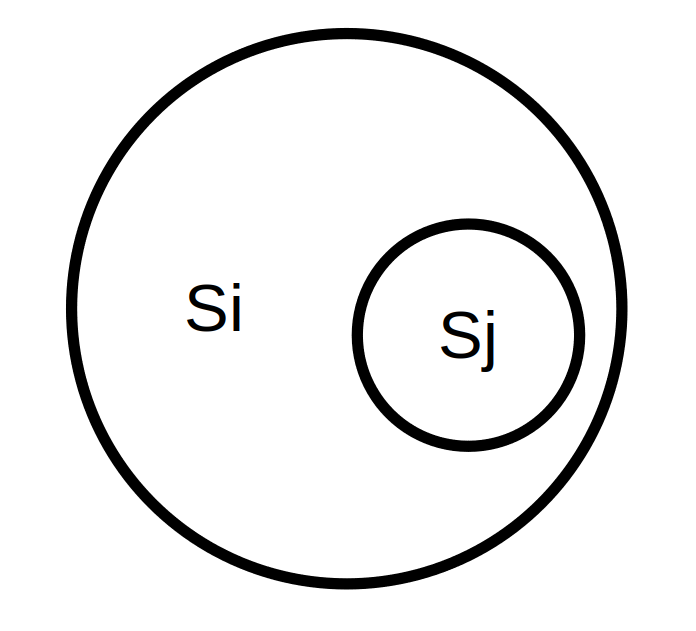
\includegraphics[width=0.4\linewidth]{figures/sd_sets/inclusion2.png}}}

\scnheader{объединение*}
\scnidtf{объединение множеств*}
\scniselement{квазибинарное отношение}
\scniselement{ориентированное отношение}
\scntext{определение}{\textbf{\textit{объединение*}} – это \textit{квазибинарное ориентированное отношение}, областью определения которого является семейство всевозможных множеств. Будем говорить, что \textit{Множество Si} является объединением \textit{Множество Sj} и \textit{Множество Sk} тогда и только тогда, когда любой элемент \textit{Множество Si} является элементом или \textit{Множество Sj} или \textit{Множество Sk}.}
\scnrelfrom{описание типичного экземпляра}{
\scnfilescg {figures/sd_sets/union.png}}
\scnaddlevel{1}
\scnnote{Множество \textit{Si} является объединением множеств \textit{Sj}, \textit{Sk} и \textit{Sm}.}
\scnaddlevel{-1}
\scnrelfrom{изображение}{
\scnfileimage{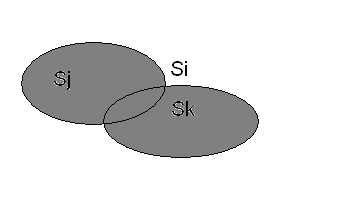
\includegraphics[width=0.6\linewidth]{figures/sd_sets/union2.png}}}

\scnheader{разбиение*}
\scnidtf{разбиение  множества*}
\scnidtf{объединение попарно непересекающихся множеств*}
\scnidtf{декомпозиция множества*}
\scniselement{квазибинарное отношение}
\scniselement{ориентированное отношение}
\scniselement{отношение декомпозиции}
\scntext{определение}{\textbf{\textit{разбиение*}} – это \textit{квазибинарное ориентированное отношение}, областью определения которого является семейство всевозможных множеств. В результате разбиения множества получается множество попарно непересекающихся множеств, объединение которых есть исходное множество.\\
Семейство множеств \{\textit{S1…, Sn}\} является разбиением множества \textit{Si} в том и только том случае, если:
\begin{scnitemize}
    \item семейство \{\textit{S1…, Sn}\} является семейством \textit{попарно непересекающихся множеств};
    \item семейство \{\textit{S1…, Sn}\} является покрытием множества \textit{Si} (или другими словами, множество \textit{Si} является \textit{объединением} множеств, входящих в указанное выше семейство)
\end{scnitemize}
}
\scnrelfrom{описание типичного экземпляра}{
\scnfilescg{figures/sd_sets/split.png}}
\scnaddlevel{1}
\scnnote{Множество \textit{Si} разбивается на множества \textit{Sj}, \textit{Sk} и \textit{Sm}.}
\scnaddlevel{-1}
\scnrelfrom{изображение}{
\scnfileimage{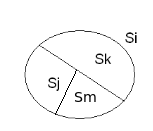
\includegraphics[width=0.5\linewidth]{figures/sd_sets/split2.png}}}

\scnheader{пересечение*}
\scnidtf{пересечение множеств*}
\scniselement{квазибинарное отношение}
\scniselement{ориентированное отношение}
\scntext{определение}{\textbf{\textit{пересечение*}} – это операция над множествами, аргументами которой являются два или большее число множеств, а результатом является множество, элементами которого являются все те и только те сущности, которые одновременно принадлежат каждому множеству, которое входит в семейство аргументов этой операции.\\
Будем говорить, что \textit{Множество Si} является пересечением \textit{Множество Sj} и \textit{Множество Sk} тогда и только тогда, когда любой элемент \textit{Множество Si} является элементом \textit{Множество Sj} и элементом \textit{Множество Sk}.}
\scnrelfrom{описание типичного экземпляра}{
\scnfilescg{figures/sd_sets/intersection.png}}
\scnaddlevel{1}
\scnnote{Множество \textit{Si} является результатом пересечения множеств \textit{Sj}, \textit{Sk} и \textit{Sm}.}
\scnaddlevel{-1}
\scnrelfrom{изображение}{
\scnfileimage{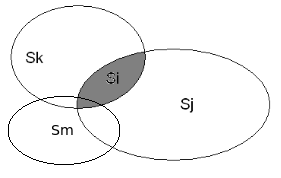
\includegraphics[width=0.5\linewidth]{figures/sd_sets/intersection2.png}}}

\scnheader{пара пересекающихся множеств*}
\scniselement{бинарное отношение}
\scniselement{неориентированное отношение}
\scnexplanation{\textbf{\textit{пара пересекающихся множеств*}} – \textit{бинарное неориентированное отношение} между двумя \textit{множествами}, имеющими непустое \textit{пересечение*}.}
\scntext{определение}{\textbf{\textit{пара пересекающихся множеств*}} – \textit{бинарное неориентированное отношение} между двумя \textit{множествами}, имеющими, по крайней мере, один общий для этих двух множеств элемент.}
\scnrelfrom{описание типичного экземпляра}{
\scnfilescg{figures/sd_sets/pairOfIntersectingSets.png}}
\scnaddlevel{1}
\scnnote{Множество \textit{Si} и множество \textit{Sj} являются парой пересекающихся множеств.}
\scnaddlevel{-1}
\scnrelfrom{изображение}{
\scnfileimage{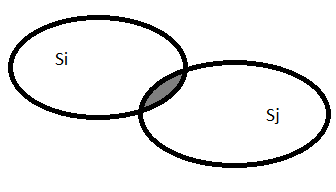
\includegraphics[width=0.5\linewidth]{figures/sd_sets/pairOfIntersectingSets2.png}}}

\scnheader{попарно пересекающиеся множества*}
\scnidtf{семейство попарно пересекающихся множеств*}
\scnsuperset{пересекающиеся множества*}
\scniselement{отношение}
\scntext{определение}{\textbf{\textit{попарно пересекающиеся множества*}} – семейство множеств, каждая пара которых является парой пересекающихся множеств, т.е. каждая пара которых имеет хотя бы один общий элемент}
\scntext{примечание}{Не каждое \textit{семейство попарно пересекающихся множеств*} является \textit{семейством пересекающихся множеств*}, хотя обратное верно.}
\scnrelfrom{изображение}{
\scnfilescg{figures/sd_sets/pairwiseIntersectingSets.png}}
\scnaddlevel{1}
\scnnote{Множества \textit{Si}, \textit{Sj}, \textit{Sk} и \textit{Sl} являются попарно пересекающимися множествами.}
\scnaddlevel{-1}
\scnrelfrom{изображение}{
\scnfileimage{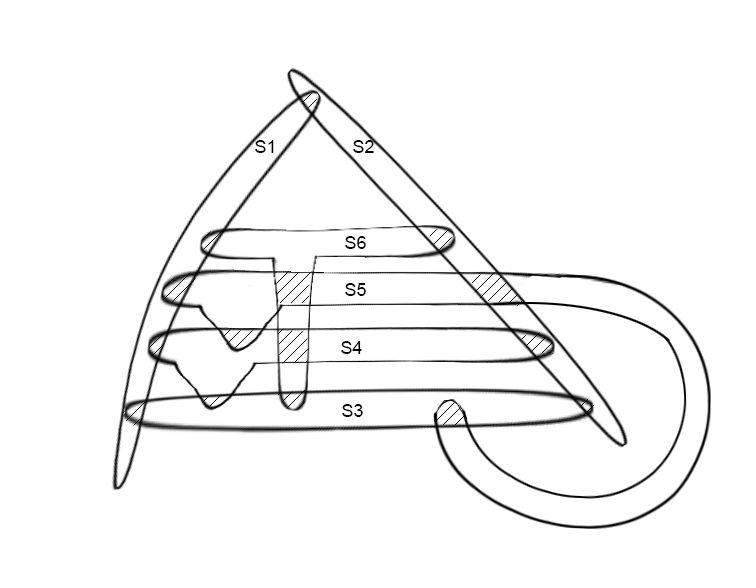
\includegraphics[width=0.7\linewidth]{figures/sd_sets/pairwiseIntersectingSets2.png}}}

\scnheader{пересекающиеся множества*}
\scnidtf{семейство пересекающихся множеств*}
\scnidtf{быть семейством пересекающихся множеств*}
\scnidtf{семейство множеств, имеющих по крайней мере один элемент, являющийся общим для всех этих множеств*}
\scnsuperset{попарно пересекающиеся множества*}
\scntext{определение}{\textbf{\textit{пересекающиеся множества*}} – это семейство множеств, имеющих по крайней мере один общий для всех этих множеств элемент}
\scnrelfrom{описание типичного экземпляра}{
\scnfilescg{figures/sd_sets/intersectingSets.png}}
\scnaddlevel{1}
\scnnote{Множества \textit{Si}, \textit{Sj}, \textit{Sk} и \textit{Sl} являются пересекающимися множествами.}
\scnaddlevel{-1}

\scnheader{пара непересекающихся множеств*}
\scniselement{бинарное отношение}
\scniselement{неориентированное отношение}
\scntext{определение}{\textbf{\textit{пара непересекающихся множеств*}} – это \textit{бинарное неориентированное отношение} между \textit{множествами}, результатом \textit{пересечения*} которых есть пустое множество.}
\scnrelfrom{описание типичного экземпляра}{
\scnfilescg{figures/sd_sets/pairOfNonIntersectingSets.png}}
\scnaddlevel{1}
\scnnote{Множества \textit{Si} и \textit{Sj} являются парой непересекающихся множеств.}
\scnaddlevel{-1}
\scnrelfrom{изображение}{
\scnfileimage{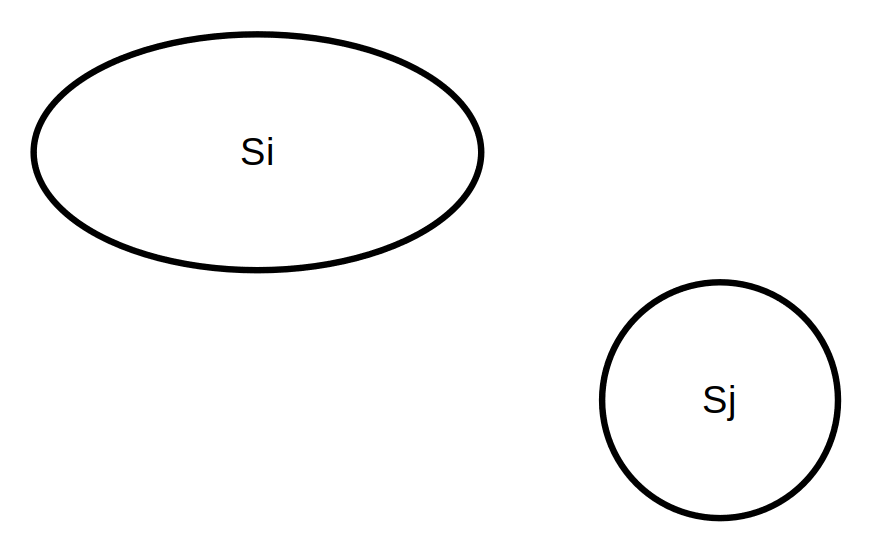
\includegraphics[width=0.5\linewidth]{figures/sd_sets/pairOfNonIntersectingSets2.png}}}

\scnheader{попарно непересекающиеся множества*}
\scnidtf{семейство попарно непересекающихся множеств*}
\scnsubset{непересекающиеся множества*}
\scntext{определение}{\textbf{\textit{попарно непересекающиеся множества*}} – семейство множеств, каждая пара которых является парой непересекающихся множеств, т.е. каждая пара которых не имеет ни одного общего элемента}
\scnrelfrom{изображение}{
\scnfilescg{figures/sd_sets/pairwiseNonIntersectingSets.png}}
\scnaddlevel{1}
\scnnote{Множества \textit{Si}, \textit{Sj}, \textit{Sk} и \textit{Sl} являются попарно непересекающимися множествами.}
\scnaddlevel{-1}

\scnheader{непересекающиеся множества*}
\scnidtf{семейство непересекающихся множеств*}
\scnidtf{быть семейством непересекающихся множеств*}
\scntext{определение}{\textbf{\textit{непересекающиеся множества*}} – это семейство множеств, не имеющих ни одного общего элемента для всех этих множеств}
\scnrelfrom{изображение}{
\scnfilescg{figures/sd_sets/nonIntersectingSets.png}
\scnnote{Множества \textit{Si}, \textit{Sj}, \textit{Sk} и \textit{Sl} являются непересекающимися множествами.}}

\scnheader{разность множеств*}
\scniselement{бинарное отношение}
\scniselement{ориентированное отношение}
\scntext{определение}{\textbf{\textit{разность множеств*}} – это \textit{бинарное ориентированное отношение}, связывающее между собой \textit{ориентированную пару}, первым элементом которой является уменьшаемое множество, вторым - вычитаемое множество, и множество, являющееся результатом вычитания вычитаемого из уменьшаемого, в которое входят все элементы первого множества, не входящие во второе множество.}
\scnrelfrom{описание типичного экземпляра}{
\scnfilescg{figures/sd_sets/setDifference.png}}
\scnaddlevel{1}
\scnnote{Множество \textit{Si} является результатом разности множеств \textit{Sj} и \textit{Sk}.}
\scnaddlevel{-1}
\scnrelfrom{изображение}{
\scnfileimage{
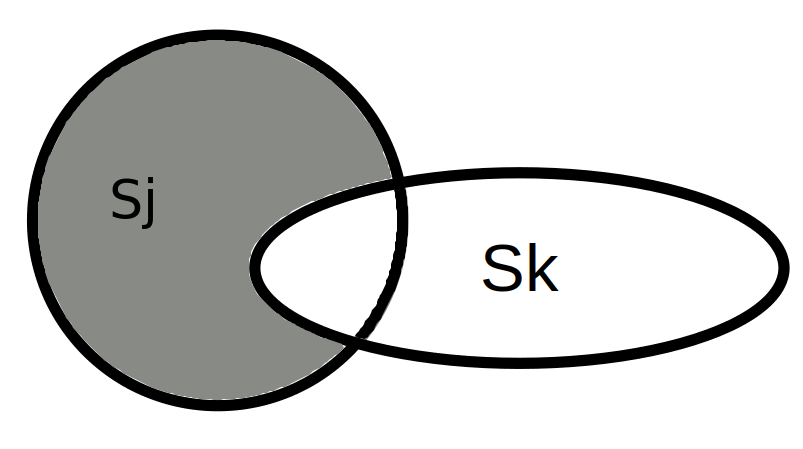
\includegraphics[width=0.5\linewidth]{figures/sd_sets/setDifference2.png}}}

\scnheader{симметрическая разность множеств*}
\scniselement{бинарное отношение}
\scniselement{ориентированное отношение}
\scntext{определение}{\textbf{\textit{симметрическая разность множеств*}} – это \textit{бинарное ориентированное отношение}, связывающее между собой \textit{пару} множеств и множество, являющееся результатом симметрической разности элементов указанной пары. Будем называть \textit{Множество Si} результатом симметрической разности \textit{Множества Sj} и \textit{Множества Sk} тогда и только тогда, когда любой элемент \textit{Множества Si} является или элементом \textit{Множества Sj} или \textit{Множества Sk}, но не является элементом обоих множеств.}
\scnrelfrom{описание типичного экземпляра}{
\scnfilescg{figures/sd_sets/symmetricDifferenceOfSets.png}
\scnnote{Множество \textit{Si} является результатом симметрической разности множеств \textit{Sj} и \textit{Sk}.}}
\scnrelfrom{изображение}{
\scnfileimage{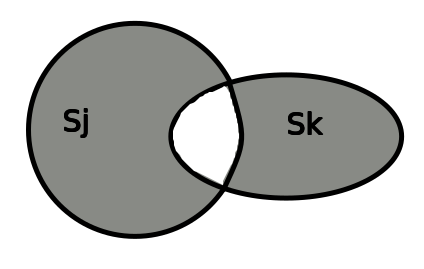
\includegraphics[width=0.5\linewidth]{figures/sd_sets/symmetricDifferenceOfSets2.png}}}

\scnheader{декартово произведение*}
\scnidtf{декартово произведение множеств*}
\scnidtf{прямое произведение множеств*}
\scniselement{бинарное отношение}
\scniselement{ориентированное отношение}
\scntext{определение}{\textbf{\textit{декартово произведение*}} – это \textit{бинарное ориентированное отношение} между \textit{ориентированной парой} множеств и \textit{множеством}, элементами которого являются всевозможные упорядоченные пары, первыми элементами которых являются элементы первого из указанных множеств, вторыми – элементы второго из указанных множеств.}
\scnrelfrom{описание типичного экземпляра}{
\scnfilescg{figures/sd_sets/cartesianMultiplication.png}}
\scnaddlevel{1}
\scnnote{Множество \textit{Si} является результатом декартова произведения множеств \textit{Sj} и \textit{Sk}.}
\scnaddlevel{-1}

\scnheader{декартово произведение}
\scnidtf{второй домен отношения быть декартовым произведением}
\scnrelfrom{второй домен}{декартово произведение*}

\scnheader{семейство подмножеств*}
\scnidtf{семейство подмножеств заданного множества*}
\scniselement{бинарное отношение}
\scniselement{ориентированное отношение}
\scnsuperset{булеан*}
\scntext{определение}{\textbf{\textit{семейство подмножеств*}} – это \textit{бинарное ориентированное отношение} между множеством и некоторым семейством множеств, каждое из которых является подмножеством первого множества.}
\scnrelfrom{описание типичного экземпляра}{
\scnfilescg{figures/sd_sets/familyOfSubsets.png}
}

\scnheader{булеан*}
\scnidtf{булеан множества*}
\scnidtf{семейство всевозможных подмножеств заданного множества*}
\scniselement{бинарное отношение}
\scniselement{ориентированное отношение}
\scntext{определение}{\textbf{\textit{булеан*}} – это \textit{бинарное ориентированное отношение} между множеством и некоторым семейством множеств, каждое из которых является подмножеством первого множества.}
\scnrelfrom{описание типичного экземпляра}{
\scnfilescg{figures/sd_sets/boulean.png}
}

\scnheader{булеан}
\scnidtf{второй домен отношения быть булеаном}
\scnrelfrom{второй домен}{булеан*}

\scnheader{мощность}
\scnidtf{мощность множеств}
\scnidtf{кардинальное число}
\scnidtf{общее число вхождений элементов в заданное множество}
\scnidtf{класс эквивалентности, элементами которого являются знаки всех тех и только тех множеств, которые имеют одинаковую мощность}
\scnidtf{класс эквивалентности, соответствующий отношению быть парой множеств, имеющих одинаковую мощность (равномощность множеств)}
\scnidtf{величина мощности множеств}
\scnidtf{трансфинитное число}
\scnidtf{мощность по Кантору}
\scniselement{параметр}
\scnexplanation{\textbf{\textit{мощность}} – это \textit{параметр}, элементами которых являются \textit{множества}, имеющие одинаковое количество элементов. Значением данного параметра является числовая величина, задающая количество элементов, входящих в данный класс множеств, т.е. по сути, количество \textit{позитивных sc-дуг принадлежности}, выходящих из данного \textit{множества}.

Для двух множеств, имеющих одинаковую мощность, существует взаимно-однозначное соответствие между ними (между множествами вхождений элементов в эти множества – на случай мультимножеств).}
\scnrelfrom{описание типичного экземпляра}{
\scnfilescg{figures/sd_sets/power.png}
}

\scnheader{равенство множеств*}
\scniselement{бинарное отношение}
\scniselement{неориентированное отношение}
\scnidtf{быть равными множествами*}
\scntext{определение}{\textbf{\textit{равенство множеств}}* - бинарное неориентированное отношение, выражающее отношение равенства множеств.

Любые два множества являются равными множествами тогда и только тогда, когда первое является включением второго и второе является включением первого.}
\scnrelfrom{описание типичного экземпляра}{
\scnfilescg{figures/sd_sets/equalityOfSets.png}}
\scnaddlevel{1}
\scnnote{Множество \textit{Si} равно множеству \textit{Sj}.}
\scnaddlevel{-1}

\scnendstruct

\end{SCn}

\scsection{Предметная область и онтология связок и отношений}
\label{sec:sd_rels}
\begin{SCn}

\scnsectionheader{\currentname}

\scnstartsubstruct

\scnheader{Предметная область связок и отношений}
\scniselement{предметная область}
\scnsdmainclasssingle{связь}
\scnsdclass{бинарная связь;sc-коннектор;неатомарная бинарная связь;небинарная связь;неориентированная связь;ориентированная связь;отношение;класс равномощных связок;класс связок разной мощности;унарное отношение;бинарное отношение;квазибинарное отношение;тернарное отношение;небинарное отношение;ориентированное отношение;неориентированное отношение;рефлексивное отношение;антирефлексивное отношение;частично рефлексивное отношение;симметричное отношение;антисимметричное отношение;частично симметричное отношение;транзитивное отношение;антитранзитивное отношение;частично транзитивное отношение;связанное отношение;отношение порядка;отношение строгого порядка;отношение нестрогого порядка;отношение толерантности;отношение эквивалентности;ролевое отношение;числовой атрибут;неролевое отношение;неролевое бинарное отношение;арность;метаотношение;отношение декомпозиции;отношение интеграции}
\scnsdrelation{область определения*;атрибут отношения*;домен*;первый домен*;второй домен*;композиция отношений*;фактор-множество*;соответствие*;отношение соответствия*;область отправления';область прибытия’;образ';прообраз';всюду определенное соответствие*;частично определенное соответствие*;сюръективное соответствие*;несюръективное соответствие*;однозначное соответствие*;обратное соответствие*;обратимое соответствие*;неоднозначное соответствие*;инъективное соответствие*;взаимно однозначное соответствие*;множество сочетаний*;множество размещений*;множество перестановок*}

\scnheader{связь}
\scnidtf{связка sc-элементов}
\scnidtf{sc-связка}
\scnexplanation{\textbf{\textit{связь}} – множество, являющееся абстрактной моделью связи между описываемыми сущностями, которые или знаки которых являются элементами этого множества.}
\scntext{примечание}{Напомним, что все элементы множества, представленного в SC-коде, являются знаками, но описываемыми сущностями могут быть не только сущности, обозначаемые sc-элементами, но и сами эти sc-элементы.}
\scnsubdividing{бинарная связь;небинарная связь}
\scnsubdividing{неориентированная связь;ориентированная связь}

\scnheader{бинарная связь}
\scnsubdividing{sc-коннектор;неатомарная бинарная связь}
\scntext{примечание}{Данное разбиение осуществляется на основе синтаксического признака, а не семантического, поскольку каждый \textit{sc-коннектор} может быть записан в памяти при помощи семантически эквивалентной конструкции, содержащей знак самой связи и пары принадлежности, ведущие к ее элементам, уточненные, при необходимости ролевыми отношениями.}

\scnheader{sc-коннектор}
\scnidtf{атомарная бинарная связь}
\scnexplanation{Каждый \textbf{\textit{sc-коннектор}} представлен в \textit{sc-памяти} одним \textit{sc-элементом} и семантически эквивалентен конструкции, содержащей знак некоторой \textit{бинарной связи} и пары принадлежности, ведущие к элементам этой связи, уточненные, при необходимости ролевыми отношениями.

Такая конструкция может быть обозначена \textbf{\textit{sc-коннектором}} только в случае, когда роли компонентов соответствующей бинарной связи указываются только при помощи \textit{числовых атрибутов 1’} и \textit{2’} или не уточняются вообще.}

\scnheader{неатомарная бинарная связь}
\scnexplanation{\textbf{\textit{неатомарная бинарная связь}} – \textit{бинарная связь}, роли компонентов которой не могут быть заданы только при помощи \textit{ролевых отношений 1'} и \textit{2'}, или не заданы совсем, а требуют дополнительного уточнения при помощи более частных ролевых отношений.}

\scnheader{небинарная связь}
\scnexplanation{\textbf{\textit{небинарная связь}} – связь, имеющая больше двух элементов.}

\scnheader{неориентированная связь}
\scnsuperset{неориентированное множество}
\scnexplanation{\textbf{\textit{неориентированная связь}} – связь, все элементы которой имеют одинаковые роли (при этом соответствующее ролевое отношение, как правило, явно не указывается).}

\scnheader{ориентированная связь}
\scnsuperset{ориентированное множество}
\scnexplanation{\textbf{\textit{ориентированная связь}} – связь, в которой с помощью ролевых отношений, указываются роли компонентов этой связи.}

\scnheader{отношение}
\scnidtf{класс связей}
\scnidtf{класс sc-связок}
\scnidtf{множество отношений}
\scnidtf{Множество всевозможных отношений}
\scntext{определение}{\textbf{\textit{отношение}}, \textit{заданное на множестве M} – это подмножество \textit{декартового произведения} этого множества самого на себя некоторое количество раз.

В более широком смысле \textbf{\textit{отношение}} – это математическая структура, которая формально определяет свойства различных объектов и их взаимосвязи.}
\scnsubdividing{класс равномощных связок;класс связок разной мощности}
\scnsubdividing{бинарное отношение;небинарное отношение}
\scnsubdividing{ориентированное отношение;неориентированное отношение}
\scnsubdividing{ролевое отношение;неролевое отношение}

\scnheader{класс равномощных связок}
\scnidtf{класс связок фиксированной арности}
\scnidtf{отношение, обладающее свойством арности}
\scnsuperset{унарное отношение}
\scnsuperset{бинарное отношение}
\scnsuperset{тернарное отношение}
\scntext{определение}{\textbf{\textit{класс равномощных связок}} – класс связок, имеющих одинаковую мощность.}

\scnheader{класс связок разной мощности}
\scnidtf{отношение нефиксированной арности}
\scnsubset{небинарное отношение}
\scntext{определение}{\textbf{\textit{класс связок разной мощности}} – класс связок, имеющих разную мощность.}

\scnheader{унарное отношение}
\scnidtf{отношение арности один}
\scnidtf{одноместное отношение}
\scnidtf{множество синглетонов}
\scntext{определение}{\textbf{\textit{унарное отношение}} – это множество таких отношений на множестве M, являющихся любым подмножеством множества M.}

\scnheader{бинарное отношение}
\scnidtf{отношение арности два}
\scnidtf{двухместное отношение}
\scnsuperset{квазибинарное отношение}
\scnsuperset{отношение порядка}
\scnsuperset{отношение толерантности}
\scnsubdividing{рефлексивное отношение;антирефлексивное отношение;частично рефлексивное отношение}
\scnsubdividing{симметричное отношение;антисимметричное отношение;частично симметричное отношение}
\scnsubdividing{транзитивное отношение;антитранзитивное отношение;частично транзитивное отношение}
\scnsubdividing{ролевое отношение;неролевое бинарное отношение}
\scntext{определение}{\textbf{\textit{бинарное отношение}} – это множество таких отношений на множестве \textbf{\textit{M}}, являющихся подмножеством \textit{декартова произведения} множества \textbf{\textit{M}}.\\
Если \textbf{\textit{бинарное отношение R}} задано на \textit{множестве} \textbf{\textit{М}} и два элемента этого множества \textbf{\textit{a}} и \textbf{\textit{b}} связаны данным отношением, то будем обозначать такую связь как \textbf{\textit{aRb}}.}

\scnheader{квазибинарное отношение}
\scnexplanation{\textbf{\textit{квазибинарное отношение}} – множество ориентированных пар, первые компоненты которых являются связками.\\
Таким образом, \textit{sc-дуги}, принадлежащие \textbf{\textit{квазибинарным отношениям}}, всегда выходят из связок.}
\scntext{sc-утверждение}{В область определения квазибинарного отношения будем включать:
\begin{scnitemize}
    \item вторые компоненты ориентированных пар, принадлежащих этому отношению;
    \item элементы первых компонентов ориентированных пар, принадлежащих этому отношению;
    \item других элементов область определения квазибинарного отношения не содержит.
\end{scnitemize}
}

\scnheader{тернарное отношение}
\scnidtf{отношение арности три}
\scnidtf{трехместное отношение}
\scnexplanation{\textbf{\textit{тернарное отношение}} – это множество отношений, связывающих между собой три элемента.}

\scnheader{небинарное отношение}
\scnexplanation{\textbf{\textit{небинарное отношение}} – это множество отношений, хотя бы одна из связок каждого из которых имеет значение мощности больше двух.}

\scnheader{ориентированное отношение}
\scntext{определение}{\textbf{\textit{ориентированное отношение}} – это множество таких отношений, каждая связка которых является ориентированным множеством.}

\scnheader{неориентированное отношение}
\scntext{определение}{\textbf{\textit{неориентированное отношение}} – это множество таких отношений, каждая связка которых является неориентированным множеством.}

\scnheader{рефлексивное отношение}
\scntext{определение}{\textbf{\textit{рефлексивное отношение}} – это \textit{бинарное отношение}, любая пара которого есть канторовское множество.}

\scnheader{антирефлексивное отношение}
\scntext{определение}{\textbf{\textit{антирефлексивное отношение R}} на \textit{множестве} \textbf{\textit{A}} – это \textit{бинарное отношение}, в котором все элементы множества \textbf{\textit{A}} не находятся в отношении \textbf{\textit{R}} к самому себе.}

\scnheader{частично рефлексивное отношение}
\scntext{определение}{\textbf{\textit{частично рефлексивное отношение R}} на \textit{множестве} \textbf{\textit{A}} – это \textit{бинарное отношение},  в котором хотя бы один (но не все) элемент множества \textbf{\textit{A}} находится в отношении \textbf{\textit{R}} к самому себе.}

\scnheader{симметричное отношение}
\scntext{определение}{\textbf{\textit{симметричное отношение R}} на \textit{множестве} \textbf{\textit{A}} – это \textit{бинарное отношение}, в котором для каждой пары элементов \textbf{\textit{а}} и \textbf{\textit{b}} этого множества выполнение отношения \textbf{\textit{aRb}} влечёт выполнение \textbf{\textit{bRa}}.}

\scnheader{антисимметричное отношение}
\scntext{определение}{\textbf{\textit{антисимметричное отношение R}} на \textit{множестве} \textbf{\textit{A}} – это \textit{бинарное отношение}, в котором для каждой пары элементов \textbf{\textit{а}} и \textbf{\textit{b}} этого множества выполнение отношений \textbf{\textit{aRb}} и \textbf{\textit{bRa}} влечёт равенство \textbf{\textit{a}} и \textbf{\textit{b}}.}

\scnheader{частично симметричное отношение}
\scntext{определение}{\textbf{\textit{частично симметричное отношение R}} на \textit{множестве} \textbf{\textit{A}} – это \textit{бинарное отношение}, в котором для каждой пары элементов \textbf{\textit{а}} и \textbf{\textit{b}} (но не для всех таких пар) этого множества выполнение отношения \textbf{\textit{aRb}} влечёт выполнение \textbf{\textit{bRa}}.}

\scnheader{транзитивное отношение}
\scntext{определение}{\textbf{\textit{транзитивное отношение R}} на \textit{множестве} \textbf{\textit{A}} – это \textit{бинарное отношение}, в котором для любых трёх элементов этого множества \textbf{\textit{a, b, c}} выполнение отношений \textbf{\textit{aRb}} и \textbf{\textit{bRc}} влечёт выполнение отношения \textbf{\textit{aRc}}.}

\scnheader{антитранзитивное отношение}
\scntext{определение}{\textbf{\textit{антитранзитивное отношение R}} на \textit{множестве} \textbf{\textit{A}} – это \textit{бинарное отношение}, в котором для любых трёх элементов этого множества \textbf{\textit{a, b, c}} выполнение отношений \textbf{\textit{aRb}} и \textbf{\textit{bRc}} не влечёт выполнение отношения \textbf{\textit{aRc}}.}

\scnheader{частично транзитивное отношение}
\scntext{определение}{\textbf{\textit{частично транзитивное отношение R}} на \textit{множестве} \textbf{\textit{A}} – это \textit{бинарное отношение}, в котором для каждых трёх элементов этого множества \textbf{\textit{a, b, c}} (но не для всех таких троек) выполнение отношений \textbf{\textit{aRb}} и \textbf{\textit{bRc}} влечёт выполнение отношения \textbf{\textit{aRc}}.}

\scnheader{связанное отношение}
\scnsubset{бинарное отношение}
\scntext{определение}{\textbf{\textit{связанное отношение R}} на \textit{множестве} \textbf{\textit{A}} – это \textit{бинарное отношение}, в котором для каждой пары элементов \textbf{\textit{а}} и \textbf{\textit{b}} этого множества выполняется одно из двух отношений: \textbf{\textit{aRb}} или \textbf{\textit{bRa}}.}

\scnheader{отношение порядка}
\scnsubdividing{отношение строгого порядка;отношение нестрогого порядка}
\scntext{определение}{\textbf{\textit{отношение порядка}} – это \textit{бинарное отношение}, обладающее свойством транзитивности и антисимметричности.}

\scnheader{отношение строгого порядка}
\scntext{определение}{\textbf{\textit{отношение строгого порядка}} – это \textit{отношение порядка}, обладающее свойством антирефлексивности.}

\scnheader{отношение нестрогого порядка}
\scntext{определение}{\textbf{\textit{отношение нестрогого порядка}} – это \textit{отношение порядка}, обладающее свойством рефлексивности.}

\scnheader{отношение толерантности}
\scntext{определение}{\textbf{\textit{отношение толерантности}} – это \textit{бинарное отношение}, принадлежащее классам \textit{симметричное отношение} и \textit{рефлексивное отношение}.}

\scnheader{отношение эквивалентности}
\scnidtf{максимальное семейство отношений эквивалентности}
\scnsubset{отношение толерантности}
\scntext{определение}{\textbf{\textit{отношение эквивалентности}} – это \textit{отношение толерантности}, принадлежащее классу \textit{транзитивных отношений}}
\scntext{примечание}{Каждое отношение эквивалентности уточняет то, что мы считаем эквивалентными сущностями, т.е. то, на какие сходства этих сущностей мы обращаем внимание и какие их отличия мы игнорируем (не учитываем).}

\scnheader{ролевое отношение}
\scnidtf{атрибут}
\scnidtf{атрибутивное отношение}
\scnidtf{отношение, которое задает роль элементов в рамках некоторого множества}
\scnidtf{отношение, являющееся подмножеством отношения принадлежности}
\scnrelto{семейство подмножеств}{принадлежность*}
\scnsubset{бинарное отношение}
\scnsuperset{числовой атрибут}
\scnexplanation{\textbf{\textit{ролевое отношение}} – это отношение, являющееся подмножеством отношения принадлежности.}
\scntext{правило идентификации экземпляров}{В конце каждого \textit{идентификатора}, соответствующего экземплярам класса \textbf{\textit{ролевое отношение}}, не являющегося системным, ставится знак «'».

Например:\\
\textit{ключевой экземпляр’}

Из-за ограничений в разрешенном алфавите символов, в системном идентификаторе не может быть использовать знак «'», поэтому в начале каждого \textit{системного идентификатора}, соответствующего экземплярам класса \textbf{\textit{ролевое отношение}} ставится префикс «rrel\_».

Например:\\
\textit{rrel\_key\_sc\_element}}

\scnheader{числовой атрибут}
\scnidtf{порядковый номер}
\scnidtf{номер компонента ориентированной связки}
\scnhaselement{1’; 2’; 3’; 4’; 5’; 6’; 7’; 8’; 9’; 10’}
\scnexplanation{\textbf{\textit{числовой атрибут}} – \textit{ролевое отношение}, задающее порядковый номер элемента некоторой ориентированной связки, не уточняя при этом семантику такой принадлежности. Во многих случаях бывает достаточно использовать числовые атрибуты, чтобы различать компоненты связки, семантика каждого из которых дополнительно оговаривается, например, при определении отношения, которому данная связка принадлежит.}

\scnheader{неролевое отношение}
\scnsubdividing{небинарное отношение;неролевое бинарное отношение}
\scnexplanation{\textbf{\textit{неролевое отношение}} – отношение, не являющееся подмножеством отношения принадлежности.}
\scntext{правило идентификации экземпляров}{В конце каждого \textit{идентификатора}, соответствующего экземплярам класса \textbf{\textit{неролевое отношение}}, не являющегося системным, ставится знак «*».

Например:\\
\textit{включение*}

Из-за ограничений в разрешенном алфавите символов, в системном идентификаторе не может быть использовать знак «*», поэтому в начале каждого \textit{системного идентификатора}, соответствующего экземплярам класса \textbf{\textit{неролевое отношение}} ставится префикс «nrel\_».

Например:\\
\textit{nrel\_inclusion}}

\scnheader{неролевое бинарное отношение}
\scnexplanation{\textbf{\textit{неролевое бинарное отношение}} – \textit{бинарное отношение}, не являющееся \textit{ролевым отношением}.}

\scnheader{арность}
\scnidtf{арность отношения}
\scniselement{параметр}
\scnexplanation{\textbf{\textit{арность}} – это параметр, каждый элемент которого представляет собой класс \textit{отношений}, каждая связка которых имеет одинаковую \textit{мощность}. Значение данного \textit{параметра} совпадает со значением \textit{мощности} каждой из таких связок.}
\scnrelfrom{описание типичного экземпляра}{
\scnfilescg{figures/sd_relations/arity.png}}


\scnheader{область определения*}
\scnidtf{область определения отношения*}
\scniselement{бинарное отношение}
\scnexplanation{\textbf{\textit{область определения*}} – это \textit{бинарное отношение}, связывающее отношение со множеством, являющимся его областью определения.

Областью определения отношения будем называть результат теоретико-множественного объединения всех связок этого отношения, или, другими словами, результат теоретико-множественного объединения всех множеств, являющихся доменами данного отношения.}
\scnrelfrom{описание типичного экземпляра}{
\scnfilescg{figures/sd_relations/domain.png}}

\scnheader{атрибут отношения*}
\scnidtf{ролевой атрибут, используемый в связках заданного отношения*}
\scniselement{бинарное отношение}
\scnexplanation{\textbf{\textit{атрибут отношения*}} – это \textit{бинарное отношение}, связывающее заданное отношение с \textit{ролевым отношением}, используемым в данном отношении для уточнения роли того или иного элемента связок данного отношения.}
\scnrelfrom{описание типичного экземпляра}{
\scnfilescg{figures/sd_relations/relationshipAttribute.png}}


\scnheader{домен*}
\scnidtf{домен отношения по заданному атрибуту*}
\scniselement{бинарное отношение}
\scnexplanation{\textbf{\textit{домен*}} – это \textit{бинарное отношение}, связывающее связку отношения \textit{атрибут отношения*} со множеством, являющимся доменом заданного отношения по заданному атрибуту. Множество \textbf{\textit{di}} является доменом отношения \textbf{\textit{ri}} по атрибуту \textbf{\textit{ai}} в том и только том случае, если элементами этого множества являются все те и только те элементы связок отношения \textbf{\textit{ri}}, которые имеют в рамках этих связок атрибут \textbf{\textit{ai}}.}
\scnrelfrom{описание типичного экземпляра}{
\scnfilescg{figures/sd_relations/domen.png}}


\scnheader{первый домен*}
\scniselement{бинарное отношение}
\scntext{определение}{\textbf{\textit{первый домен*}} – это \textit{бинарное отношение}, связывающее отношение с множеством, являющимся доменом по атрибуту \textbf{\textit {1'}} данного отношения.}
\scnrelfrom{описание типичного экземпляра}{
\scnfilescg{figures/sd_relations/firstDomain.png}}

\scnheader{второй домен*}
\scniselement{бинарное отношение}
\scntext{определение}{\textbf{\textit{второй домен*}} – это \textit{бинарное отношение}, связывающее отношение с множеством, являющимся доменом по атрибуту \textbf{\textit{2'}} данного отношения.}
\scnrelfrom{описание типичного экземпляра}{
\scnfilescg{figures/sd_relations/secondDomain.png}}

\scnheader{композиция отношений*}
\scniselement{квазибинарное отношение}
\scntext{определение}{\textbf{\textit{композиция отношений*}} – это \textit{квазибинарное отношение}, связывающее два бинарных отношения с отношением, являющимся их композицией. Под композицией бинарных отношений \textbf{\textit{R}} и \textbf{\textit{S}} будем понимать множество $\{(x, y) | \exists z(xSz \wedge zRy)\}$}
\scnrelfrom{описание типичного экземпляра}{
\scnfilescg{figures/sd_relations/relationshipComposition.png}}

\scnheader{фактор-множество*}
\scnidtf{быть фактор-множеством*}
\scnidtf{множество всевозможных максимальных множеств из попарно эквивалентных элементов*}
\scnidtf{множество всевозможных классов эквивалентности для заданного отношения эквивалентности*}
\scniselement{бинарное отношение}
\scntext{определение}{\textbf{\textit{фактор множество*}} - это бинарное ориентированное отношение, каждая связка которого связывает некоторое отношение эквивалентности со множеством всех соответствующих этому отношению классов эквивалентности. Каждый такой класс представляет собой максимальное множество сущностей, каждая пара которых принадлежит указанному выше отношению эквивалентности.}
\scnrelfrom{описание типичного экземпляра}{
\scnfilescg{figures/sd_relations/factor_set.png}}

\scnheader{метаотношение}
\scntext{определение}{метаотношение - это \textit{отношение}, в каждой связке которого есть по крайней мере один компонент, являющийся знаком некоторого \textit{отношения}.}

\scnheader{отношение декомпозиции}
\scnhaselement{разбиение*}
\scnhaselement{декомпозиция раздела*}
\scnhaselement{декомпозиция абстрактного объекта*}

\scnheader{отношение интеграции}
\scnhaselement{объединение*}

\scnheader{соответствие*}
\scnidtf{наличие соответствия*}
\scniselement{бинарное отношение}
\scnsubdividing{соответствие между непересекающимися множествами*;соответствие между строго пересекающимися множествами*;соответствие, область отправления и область прибытия которого совпадают*}
\scnsubdividing{всюду определенное соответствие*;частично определенное соответствие*}
\scnsubdividing{сюръекция*;несюръективное соответствие*}
\scnsubdividing{однозначное соответствие*;неоднозначное соответствие*}
\scntext{определение}{\textbf{\textit{соответствие*}} – \textit{бинарное отношение}, заданное на множествах и задающее наличие отношения, в котором участвуют только элементы этих множеств.}
\scnrelfrom{описание типичного экземпляра}{
\scnfilescg{figures/sd_relations/conformity.png}}

\scnheader{отношение соответствия*}
\scniselement{бинарное отношение}
\scntext{определение}{\textbf{\textit{отношение соответствия*}} – \textit{бинарное отношение}, связывающее ориентированную пару множеств, на которых задано \textit{соответствие*} и некоторое подмножество \textit{декартова произведения*} этих \textit{множеств}.}
\scnrelfrom{описание типичного экземпляра}{
\scnfilescg{figures/sd_relations/relationshipConformity.png}}

\scnheader{область отправления'}
\scnidtf{область отправления соответствия’}
\scnidtf{область определения соответствия’}
\scnidtf{первый компонент пары в отношении соответствия’}
\scniselement{ролевое отношение}
\scntext{определение}{\textbf{\textit{область отправления'}} – \textit{ролевое отношение}, указывающее на первый компонент пары в рамках отношения \textit{соответствие*}.}
\scnrelfrom{описание типичного экземпляра}{
\scnfilescg{figures/sd_relations/departureArea.png}}

\scnheader{область прибытия’}
\scnidtf{область прибытия соответствия'}
\scnidtf{область значений соответствия'}
\scniselement{ролевое отношение}
\scntext{определение}{\textbf{\textit{область прибытия’}} – \textit{ролевое отношение}, указывающее на второй компонент пары в рамках отношения \textit{соответствие*}.}
\scnrelfrom{описание типичного экземпляра}{
\scnfilescg{figures/sd_relations/arrivalArea.png}}

\scnheader{образ'}
\scnidtf{образ соответствия’}
\scniselement{ролевое отношение}
\scntext{определение}{\textbf{\textit{образ'}} – \textit{ролевое отношение}, указывающее на второй компонент каждой пары в рамках множества пар, которое является вторым компонентом \textit{отношения соответствия*}.}
\scnrelfrom{описание типичного экземпляра}{
\scnfilescg{figures/sd_relations/form.png}}

\scnheader{прообраз'}
\scnidtf{прообраз соответствия’}
\scniselement{ролевое отношение}
\scntext{определение}{\textbf{\textit{прообраз'}} – \textit{ролевое отношение}, указывающее на первый компонент каждой пары в рамках множества пар, которое является первым компонентом \textit{отношения соответствия*}.}
\scnrelfrom{описание типичного экземпляра}{
\scnfilescg{figures/sd_relations/prototype.png}}

\scnheader{всюду определенное соответствие*}
\scnidtf{полное соответствие*}
\scnidtf{наличие всюду определенного соответствия*}
\scntext{определение}{\textbf{\textit{всюду определенное соответствие*}} – это \textit{соответствие*}, при котором существует \textit{образ’} для каждого элемента \textit{области отправления'} данного \textit{соответствия*}.}
\scnrelfrom{описание типичного экземпляра}{
\scnfilescg{figures/sd_relations/surjection.png}}
\scnrelfrom{изображение}{
\scnfileimage{
\includegraphics[width=0.5\linewidth]{figures/sd_relations/surjection2.png}}}


\scnheader{частично определенное соответствие*}
\scnidtf{наличие частично определенного соответствия*}
\scntext{определение}{\textbf{\textit{частично определенное соответствие*}} – это \textit{соответствие*}, при котором существует \textit{образ’} для некоторых, но не всех элементов \textit{области отправления'} данного \textit{соответствия*}.}
\scnrelfrom{описание типичного экземпляра}{
\scnfilescg{figures/sd_relations/partiallyDefinedConformity.png}}
\scnrelfrom{изображение}{
\scnfileimage{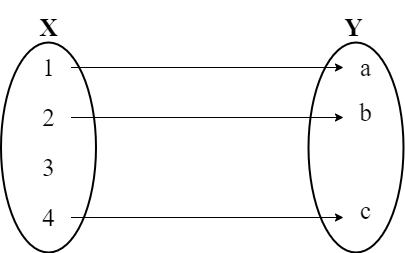
\includegraphics[width=0.5\linewidth]{figures/sd_relations/partiallySurjection.png}}}


\scnheader{сюръективное соответствие*}
\scnidtf{наличие сюръективного соответствия*}
\scnidtf{сюръекция*}
\scntext{определение}{\textbf{\textit{сюръективное соответствие*}} – это \textit{соответствие*}, при котором существует \textit{прообраз’} для каждого элемента \textit{области прибытия'} данного \textit{соответствия*}.}
\scnrelfrom{описание типичного экземпляра}{
\scnfilescg{figures/sd_relations/surjectiveConformity.png}}
\scnrelfrom{изображение}{
\scnfileimage{
\includegraphics[width=0.5\linewidth]{figures/sd_relations/surjectiveConformity2.png}}}

\scnheader{несюръективное соответствие*}
\scnidtf{наличие несюръективного соответствия*}
\scntext{определение}{\textbf{\textit{несюръективное соответствие*}} – это \textit{соответствие*}, при котором не для каждого элемента \textit{области прибытия'} данного \textit{соответствия*} существует \textit{прообраз’}.}
\scnrelfrom{описание типичного экземпляра}{
\scnfilescg{figures/sd_relations/nonSurjectiveConformity.png}}
\scnrelfrom{изображение}{
\scnfileimage{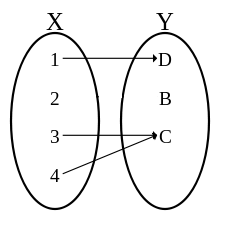
\includegraphics[width=0.5\linewidth]{figures/sd_relations/nonSurjectiveConformity2.png}}}

\scnheader{однозначное соответствие*}
\scnidtf{наличие однозначного соответствия*}
\scnidtf{функциональное соответветствие*}
\scnidtf{функция*}
\scntext{определение}{\textbf{\textit{однозначное соответствие*}} – это \textit{соответствие*}, при котором каждому элементу из \textit{области отправления'} соответствия ставится не более, чем один элемент из \textit{области прибытия’} соответствия.}
\scnrelfrom{описание типичного экземпляра}{
\scnfilescg{figures/sd_relations/singleConformity.png}}
\scnrelfrom{изображение}{
\scnfileimage{
\includegraphics[width=0.5\linewidth]{figures/sd_relations/singleConformity2.png}}}

\scnheader{обратное соответствие*}
\scniselement{бинарное отношение}
\scnrelfrom{область определения}{соответствие*}
\scntext{определение}{\textbf{\textit{обратное соответствие*}} – \textit{бинарное отношение}, связывающее два \textit{соответствия*}, при этом выполняются следующие условия:
\begin{scnitemize}
    \item \textit{область отправления’} первого соответствия является \textit{областью прибытия'} второго;
    \item \textit{область прибытия’} первого соответствия является \textit{областью отправления'} второго;
    \item для каждой пары, входящей в состав отношения первого соответствия, существует пара, входящая в состав отношения второго соответствия, при этом \textit{образ’} и \textit{прообраз'} в рамках первой указанной пары являются соответственно \textit{прообразом'} и \textit{образом’} в рамках второй.
\end{scnitemize}
}

\scnheader{обратимое соответствие*}
\scnsubset{однозначное соответствие*}
\scntext{определение}{\textbf{\textit{обратимое соответствие*}} – такое \textit{однозначное соответствие*}, для которого \textit{обратное соответствие*} также является \textit{однозначным соответствием*}.}

\scnheader{неоднозначное соответствие*}
\scntext{определение}{\textbf{\textit{неоднозначное соответствие*}} – это \textit{соответствие*}, при котором хотя бы одному элементу из \textit{области отправления’} соответствия ставится более, чем один элемент из \textit{области прибытия'} соответствия.}
\scnrelfrom{описание типичного экземпляра}{
\scnfilescg{figures/sd_relations/nonSingleConformity.png}}
\scnrelfrom{изображение}{
\scnfileimage{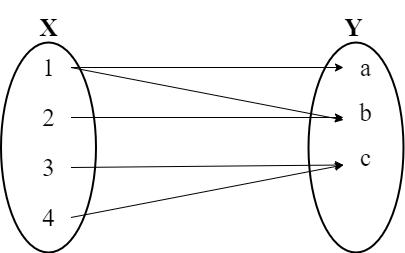
\includegraphics[width=0.5\linewidth]{figures/sd_relations/nonSingleConformity2.png}}}

\scnheader{инъективное соответствие*}
\scnidtf{инъекция*}
\scnsubset{однозначное соответствие*}
\scntext{определение}{\textbf{\textit{инъективное соответствие*}} – это \textit{соответствие*}, при котором разным элементам из \textit{области отправления’} соответствия всегда соответствуют разные элементы из \textit{области прибытия'} соответствия и наоборот.}
\scnrelfrom{описание типичного экземпляра}{
\scnfilescg{figures/sd_relations/injectiveConformity.png}}
\scnrelfrom{изображение}{
\scnfileimage{
\includegraphics[width=0.5\linewidth]{figures/sd_relations/injectiveConformity2.png}}}

\scnheader{взаимно однозначное соответствие*}
\scnidtf{биекция*}
\scnsubset{всюду определенное соответствие*}
\scnsubset{сюръективное соответствие*}
\scnsubset{инъективное соответствие*}
\scntext{определение}{\textbf{\textit{взаимно однозначное соответствие*}} – это \textit{инъективное соответствие*}, являющееся всюду определенным и сюръективным.}
\scnrelfrom{описание типичного экземпляра}{
\scnfilescg{figures/sd_relations/bijectiveConformity.png}}
\scnrelfrom{изображение}{
\scnfileimage{
\includegraphics[width=0.5\linewidth]{figures/sd_relations/bijectiveConformity2.png}}}


\scnheader{множество сочетаний*}
\scnidtf{множество всевозможных сочетаний*}
\scnidtf{множество всевозможных сочетаний заданной арности из элементов заданного множества*}
\scnidtf{множество всех неориентированных связок заданной арности*}
\scnidtf{множество всех подмножеств заданной мощности*}
\scnidtf{семейство всевозможных сочетаний*}
\scntext{определение}{\textbf{\textit{множество сочетаний*}} - \textit{отношение}, связывающее некоторое множество и семейство всевозможных множеств, имеющих значение мощности, меньше либо равное мощности исходного множества и состоящих из тех же элементов, что и это множество.}
\scntext{утверждение}{Мощность \textbf{\textit{множества сочетаний*}} может быть вычислена как n!/(k!(n-k)!), где \textbf{\textit{n}} – мощность исходного множества, \textbf{\textit{k}} – мощность элементов множества сочетаний.}
\scnrelfrom{описание типичного экземпляра}{
\scnfilescg{figures/sd_relations/setsOfCombinations.png}
\scntext{комментарий}{Для Множества \textbf{\textit{Si}} представлено множество сочетаний по 2 элемента.}}

\scnheader{множество размещений*}
\scntext{определение}{\textbf{\textit{множество размещений*}} - \textit{отношение}, связывающее некоторое множество и семейство всевозможных кортежей, имеющих значение мощности, меньше либо равное мощности исходного множества и состоящих из тех же элементов, что и это множество.}
\scntext{утверждение}{Мощность \textbf{\textit{множества сочетаний*}} может быть вычислена как n!/(n-k)!, где \textbf{\textit{n}} – мощность исходного множества, \textbf{\textit{k}} – мощность элементов множества сочетаний.}
\scnrelfrom{описание типичного экземпляра}{
\scnfilescg{figures/sd_relations/setsOfPlacements.png}
\scntext{комментарий}{Для Множества \textbf{\textit{Si}} представлено множество размещений по 2 элемента.}}

\scnheader{множество перестановок*}
\scnsubset{множество размещений*}
\scntext{определение}{\textbf{\textit{множество перестановок*}} - \textit{отношение}, связывающее некоторое множество и семейство всевозможных кортежей, равномощных исходному множеству и состоящих из тех же элементов, что и это множество.}
\scntext{утверждение}{Мощность \textbf{\textit{множества перестановок*}} может быть вычислена как n!, где \textbf{\textit{n}} – мощность исходного множества.}
\scnrelfrom{описание типичного экземпляра}{
\scnfilescg{figures/sd_relations/setsOfPermutations.png}
\scntext{комментарий}{Для Множества \textbf{\textit{Si}} представлено его множество перестановок.}}
\scnendstruct

\end{SCn}

\scsection{Предметная область и онтология параметров, величин и шкал}
\label{sec:sd_params}
\begin{SCn}

\scnsectionheader{Предметная область и онтология параметров, величин и измерений}

\scnstartsubstruct

\scnheader{Предметная область параметров, величин и измерений}
\scnidtf{Предметная область параметров и классов эквивалентности, являющихся их элементами (значениями, величинами)}
\scniselement{предметная область}
\scnsdmainclasssingle{параметр}
\scnsdclass{измеряемый параметр;неизмеряемый параметр;уровень класса эквивалентности;величина;точная величина;неточная величина;интервальная величина;параметрическая модель;измерение с фиксированной единицей измерения ;измерение по шкале;арифметическое выражение на величинах;арифметическая операция на величинах;действие. измерение;задача. измерение}
\scnsdrelation{область определения параметра*;эталон';измерение*;точность*;единица измерения*;нулевая отметка*;единичная отметка*;сумма величин*;произведение величин*;возведение величин в степень*;большая величина*;равенство величин*;большая или равная величина*}

\scnheader{параметр}
\scnidtf{характеристика}
\scnidtf{свойство}
\scnidtf{признак}
\scnidtf{класс классов}
\scnidtf{измеряемое свойство}
\scnidtf{признак классификации или покрытия некоторого класса сущностей}
\scnidtf{признак разбиения или покрытия некоторого класса сущностей}
\scnidtf{семейство множеств, разбивающих или покрывающих некоторый класс сущностей}
\scnidtf{семейство классов сущностей, обладающих одинаковым соответствующим свойством}
\scnidtf{фактор-множество, соответствующее некоторому отношению эквивалентности, или аналог фактор-множества, соответствующий некоторому отношению толерантности}
\scnreltoset{разбиение}{измеряемый параметр;неизмеряемый параметр}
\scnexplanation{Каждый \textbf{\textit{параметр}} представляет собой класс, являющийся семейством всевозможных классов эквивалентности или толерантности, задаваемых либо \textit{отношением эквивалентности}, либо \textit{отношением толерантности} (симметричным, рефлексивным, но частично транзитивным). Так, например, элементами (значениями, величинами) \textbf{\textit{параметра}} \textit{длина} являются либо классы эквивалентности, задаваемые отношением эквивалентности «иметь точно одинаковую длину*», либо классы толерантности, задаваемые отношением вида «иметь приблизительно одинаковую длину с указываемой точностью*», либо интервальные классы, задаваемые бинарными отношениями вида «иметь длину, находящуюся в одном и том же указываемом интервале*» (например, от 1 метра до 2 метров).\\
Примерами параметров как отношений эквивалентности являются:
\begin{scnitemize}
    \item равновеликость геометрических фигур (по длине, площади, объему – в зависимости от размерности этих фигур);
    \item иметь одинаковый цвет (быть эквивалентными по цвету);
    \item эквивалентность, по вкусу, запаху, твердости и т.д.
\end{scnitemize}

Заметим, что среди элементов (значений, величин) параметра могут встречаться пересекающиеся множества (классы), но объединение всех элементов каждого параметра есть не что иное, как класс всевозможных сущностей, обладающих этим параметром (свойством, характеристикой). Например, класс всех сущностей, имеющих длину, класс всех сущностей, обладающих цветом.

Каждый конкретный параметр (характеристика), т.е. каждый элемент класса всевозможных параметров (характеристик) есть, по сути, признак классификации сущностей, обладающих это характеристикой, по принципу эквивалентности (одинаковости значения) этой характеристики. Например, параметр \textit{цвет} разбивает множество сущностей имеющих цвет на классы, каждый из которых включает в себя сущности, имеющие одинаковый цвет. Параметр может разбиваться на классы для уточнения некоторого свойства, например элементами параметра цвет будут классы, соответствующие конкретным цветам (синий, красный и т.д.), в свою очередь каждый конкретный цвет может включать более частные классы, уточняющие данное свойство, например, темно-синий, светло-красный и т.д.

Другими словами, каждому множеству сущностей может ставиться в соответствие набор (семейство) параметров (параметрическое пространство), которыми обладают сущности этого множества – аналог семейства отношений, определенных (заданных) на этом множестве. Часто бывает важно построить такое параметрическое пространство, «точки» которого взаимно-однозначно соответствуют параметризуемым сущностям (например, набор параметров, позволяющих однозначно идентифицировать, установить личность каждого человека). 

Таким образом, для каждого используемого элемента (значения) какого-либо параметра, необходимо явно указывать спецификацию этого значения (точное значение, неточное значение, интервальное значение, точность, интервал).}
\scnrelfrom{типичная семантическая окрестность}{
\scnfilescg{figures/sd_parameters_and_quantities/parameterDescription.png}
}

\scnheader{область определения параметра*}
\scnidtf{множество всех тех и только тех сущностей, которые являются компонентами значений заданного параметра*}
\scnidtf{множество всех тех и только тех сущностей, которые обладают заданным параметром*}
\scnrelto{включение}{объединение*}

\scnheader{измеряемый параметр}
\scnidtf{количественный параметр}
\scnidtf{семейство измеряемых величин}
\scnidtf{семейство классов эквивалентности, каждому из которых может быть поставлено в соответствие числовое значение}
\scnexplanation{Каждый \textbf{\textit{измеряемый параметр}} представляет собой \textit{параметр}, значение (элемент, экземпляр) которого трактуется как \textit{величина}, которой можно поставить в соответствие ее числовое значение на основании выбранной единицы измерения и точки отсчета (нулевой отметки выбранной шкалы).}

\scnheader{неизмеряемый параметр}
\scnidtf{качественный параметр}

\scnheader{уровень класса эквивалентности}
\scnidtf{уровень параметра}
\scniselement{параметр}
\scnexplanation{Параметр \textbf{\textit{уровень класса эквивалентности}} задает уровень некоторого значения некоторого \textit{параметра} в иерархии значений этого параметра. Уровень класса эквивалентности равен 1, если значение параметра не является частным по отношению к другому значению этого параметра, равен 2, если значение параметра является частным по отношению к значению этого параметра с уровнем 1 и т.д.}
\scnrelfrom{типичная семантическая окрестность}{
\scnfilescg{figures/sd_parameters_and_quantities/color.png}
}

\scnheader{величина}
\scnidtf{значение количественного параметра}
\scnidtf{значение измеряемого параметра}
\scnidtf{класс сущностей, имеющих одинаковое значение соответствующего параметра}
\scnrelfromlist{включение}{точная величина;неточная величина;интервальная величина}
\scnexplanation{Каждая \textbf{\textit{величина}} представляет собой однозначный и независящий от шкалы измерения результат измерения некоторой характеристики у некоторой сущности.

Каждой \textbf{\textit{величине}} можно поставить в соответствие ее числовое значение на основании выбранной единицы измерения и точки отсчета (нулевой отметки выбранной шкалы, в случае, если измерение осуществляется по шкале).

Нельзя путать значение параметра (\textbf{\textit{величину}}) и значение величины по некоторой шкале, которое может быть скалярным и векторным.}

\scnheader{точная величина}
\scnidtf{точное значение параметра}
\scnidtf{множество всех точных значений параметра}
\scnidtf{значение параметра, являющееся семейством классов эквивалентности, соответствующим некоторому отношению эквивалентности}
\scnidtf{класс эквивалентности}
\scnexplanation{Каждая \textbf{\textit{точная величина}} имеет одно фиксированное значение в некоторой единице измерения или по какой-либо шкале. При этом считается, что все элементы такого класса имеют одинаковое значение данного параметра и отклонениями можно пренебречь.

Каждой \textbf{\textit{точной величине}} можно поставить в соответствие группу \textit{неточных величин}, являющихся не разбиениями, а покрытиями того же множества, но с разной степенью точности.}
\scnrelfrom{типичная семантическая окрестность}{
\scnfilescg{figures/sd_parameters_and_quantities/exactLength.png}
\scntext{комментарий}{В данном примере \textbf{\textit{ki}} обозначает класс сущностей, имеющих длину ровно 5 метров. Конкретный пример такой сущности - \textbf{\textit{bi}}.}}

\scnheader{неточная величина}
\scnidtf{множество неточных значений параметра}
\scnidtf{приблизительная величина}
\scnidtf{приблизительное значение параметра}
\scnidtf{значение параметра в интервале с нефиксированными границами}
\scnexplanation{Каждой \textbf{\textit{неточной величине}} ставится в соответствие ее значение в некоторой единице измерения или по какой-либо шкале, а также дополнительно указывается \textit{точность*}, т.е. возможное отклонение от данного значения.}
\scnrelfrom{типичная семантическая окрестность}{
\scnfilescg{figures/sd_parameters_and_quantities/approximateLength.png}
\scntext{комментарий}{В данном примере \textbf{\textit{ki}} обозначает класс сущностей, имеющих длину примерно 25 метров, при этом максимально возможное отклонение от этого значения составляет \textbf{\textit{kj}}, то есть 2 метра. Конкретный пример такой сущности - \textbf{\textit{bi}}.}}

\scnheader{интервальная  величина}
\scnidtf{интервальное значение параметра}
\scnidtf{значение параметра в интервале с фиксированными границами}
\scnidtf{интервал значения параметра из множества пересекающихся интервалов разной длины, имеющих нефиксированные границы}
\scnexplanation{Каждая \textbf{\textit{интервальная величина}} представляет собой класс сущностей, находящихся в рамках точно заданного интервала, минимальная и максимальная точка которого являются \textit{точными величинами}. Результатом \textit{измерения*} такой величины является ориентированная пара, первым компонентом которой является левая (меньшая) граница интервала, вторым компонентом – правая (большая) граница интервала.}
\scnrelfrom{типичная семантическая окрестность}{
\scnfilescg{figures/sd_parameters_and_quantities/intervalLength.png}
\scntext{комментарий}{В данном примере \textbf{\textit{ki}} обозначает класс сущностей, имеющих длину, которая лежит в интервале от \textbf{\textit{kj}} до \textit{kl}, то есть в интервале от 4 до 5 метров, а \textbf{\textit{bi}} – конкретный пример такой сущности.}}

\scnheader{эталон'}
\scnidtf{образец'}
\scniselement{ролевое отношение}
\scnexplanation{Ролевое отношение \textit{эталон'} указывает на тот элемент значения некоторого параметра, который в рамках данного класса эквивалентности считается эталонным, то есть он используется как образец при определении данного параметра.

\textit{эталон'} может задаваться как для измеряемых, так и для неизмеряемых параметров, например, эталон метра или эталон красоты.}

\scnheader{измерение*}
\scnidtf{значение параметра*}
\scnidtf{значение величины*}
\scnidtf{измерение как соответствие*}
\scnidtf{результат измерения заданной величины в заданной единице измерения и по заданной шкале*}
\scnidtf{бинарное ориентированное отношение, связывающее различные величины с результатами их измерения в различных единицах измерения и по различным шкалам*}
\scnexplanation{Связки отношения \textit{измерение*} связывают величину и ее значение в некоторой единице измерения (в том числе, в интервале) или по некоторой шкале. Конкретная единица измерения или шкала указывается дополнительно при помощи соответствующего отношения. Одной величине может соответствовать только одно значение в каждой возможной единице измерения или одна точка на некоторой шкале.}

\scnheader{точность*}
\scnidtf{отклонение*}
\scnidtf{степень точности неточного значения параметра*}
\scniselement{бинарное отношение}
\scnexplanation{Связки отношения \textbf{\textit{точность*}} связывают \textit{неточную величину} и \textit{точную величину} того же класса, задающую максимальное возможное отклонение указанной \textit{неточной величины} от своего значения.}

\scnheader{параметрическая модель}
\scnidtf{параметрическая спецификация}
\scnidtf{параметрическое sc-описание заданной сущности}
\scnidtf{описание сущности как точки в некотором параметрическом (признаковом) пространстве}
\scnrelto{включение}{семантическая окрестность}
\scnexplanation{Каждая \textbf{\textit{параметрическая модель}} представляет собой описание заданной сущности в некотором параметрическом пространстве количественных и качественных \textit{параметров}, т.е. указание того, какие значения заданных параметров (характеристик) соответствуют описываемой (заданной) сущности.}

\scnheader{единица измерения*}
\scniselement{бинарное отношение}
\scnexplanation{Связки отношения \textbf{\textit{единица измерения*}} связывают знак конкретного \textbf{\textit{измерения с фиксированной единицей измерения}} и некоторую \textit{точную величину}, входящую в тот же конкретный \textit{параметр}, что и первый компонент связок этого конкретного измерения, и которая используется в данном случае в качестве единицы измерения.}

\scnheader{измерение с фиксированной единицей измерения }
\scnrelto{семейство подмножеств}{измерение*}
\scnexplanation{Каждая \textbf{\textit{измерение с фиксированной единицей измерения}} представляет собой подмножество отношения \textit{измерение*} и характеризуется некоторой \textit{единицей измерения*}, которая является элементом того же параметра (семейством сущностей, имеющих значение данного параметра, совпадающее с этой единицей измерения).}

\scnheader{измерение по шкале }
\scnidtf{шкала}
\scnrelto{семейство подмножеств}{измерение*}
\scnexplanation{Каждая \textbf{\textit{измерение по шкале}} представляет собой подмножество отношения \textit{измерение*} и характеризуется не единицей измерения, а некоторой точкой отсчета для данной \textbf{\textit{шкалы}}. Результатом \textbf{\textit{измерения по шкале}} будет некоторая точка шкалы, отстоящая от точки отсчета на определенное расстояние в нужную сторону (меньшую или большую). Понятно, что это расстояние может быть измерено любыми единицами измерения, но его величина при этом останется неизменной.

Не стоит путать измерение по \textbf{\textit{измерение по шкале}}, которое зависит от \textit{нулевой отметки*}, с измерением изменения того же \textit{параметра}, которое характеризуется единицей измерения и не зависит от точки отсчета. Например, не стоит путать дату по некоторому календарю, соответствующую \textit{началу} какого-либо процесса, и \textit{длительность} этого процесса, которая не зависит от выбранного календаря.}
\scnrelfrom{типичная семантическая окрестность}{
\scnfilescg{figures/sd_parameters_and_quantities/scale.png}
\scntext{комментарий}{В данном примере \textbf{\textit{ki}} обозначает класс сущностей, имеющих точную температуру в 330 К, а \textbf{\textit{bi}} – конкретный пример такой сущности.}}

\scnheader{нулевая отметка*}
\scnidtf{нуль по шкале*}
\scnidtf{начало отсчета*}
\scniselement{бинарное отношение}
\scnexplanation{Связки отношения \textbf{\textit{нулевая отметка*}} связывают знак некоторого \textit{измерения по шкале} со знаком \textit{точной величины} того же \textit{параметра}, которая в рамках данной шкалы принимается за точку отсчета.}

\scnheader{единичная отметка*}
\scnidtf{единица по шкале*}
\scniselement{бинарное отношение}
\scnexplanation{Связки отношения \textbf{\textit{единичная отметка*}} связывают знак некоторого \textit{измерения по шкале} со знаком \textit{точной величины} того же \textit{параметра}, которая в рамках данной шкалы принимается за единичную отметку, т.е. отметку шкалы, отстоящую от нулевой на расстояние, равное выбранной единице измерения. Вместо указания единичной отметки можно использовать указание единицы измерения, однако величина, выбранная в качестве единицы измерения в этом случае будет принадлежать другому измеряемому параметру, характеризующему \uline{изменение} значения величины параметра, измеряемого по шкале.}

\scnheader{арифметическое выражение на величинах}
\scnexplanation{Каждое \textbf{\textit{арифметическое выражение на величинах}} представляет собой \textit{связку}, компонентами которой являются элементы или подмножества некоторого \textit{количественного параметра}.}

\scnheader{арифметическая операция на величинах}
\scnrelto{семейство подмножеств}{арифметическое выражение на величинах}
\scnexplanation{Каждая \textbf{\textit{арифметическая операция на величинах}} представляет собой \textit{отношение}, элементами которого являются \textit{арифметические выражения на величинах}, то есть множество \textit{арифметических выражений на величинах} какого-либо одного вида.}

\scnheader{сумма величин*}
\scnidtf{сложение величин*}
\scniselement{арифметическая операция на величинах}
\scniselement{квазибинарное отношение}
\scnexplanation{\textbf{\textit{сумма величин*}} – это \textit{арифметическая операция на величинах}, аналогичная \textit{арифметической операции сумма*} для \textit{чисел}.

Первым компонентом связки отношения \textbf{\textit{сумма величин*}} является подмножество некоторого \textit{количественного параметра} (слагаемые \textit{величины}), содержащее два или более элемента, вторым компонентом – элемент этого же \textit{количественного параметра}, значение которого в любой \textit{единице измерения*} является результатом сложения значений всех слагаемых \textit{величин} в той же \textit{единице измерения*}. При несовпадении \textit{единиц измерения} слагаемых величин необходимо воспользоваться соотношениями между \textit{единицами измерения}, которые задаются при помощи операций \textit{произведение величин*} и \textit{возведение величин в степень*}.}


\scnheader{произведение величин*}
\scnidtf{умножение величин*}
\scniselement{арифметическая операция на величинах}
\scniselement{квазибинарное отношение}
\scnexplanation{\textbf{\textit{произведение величин*}} – это \textit{арифметическая операция на величинах}, аналогичная \textit{арифметической операции произведение*} для \textit{чисел}.

Первым компонентом связки отношения \textbf{\textit{произведение величин*}} является \textit{связка}, элементами которой являются либо \textit{величины количественных параметров}, либо \textit{числа}, но при этом хотя бы один элемент должен быть \textit{величиной}. Вторым компонентов является \textit{величина количественного параметра}.

Операция \textbf{\textit{произведение величин*}} может быть использована для задания соотношения между \textit{единицами измерения*} в рамках одного \textit{количественного параметра}.}
\scnrelfrom{описание типичного экземпляра}{
\scnfilescg{figures/sd_parameters_and_quantities/multiplicationOfQuantities.png}}

\scnrelfrom{описание типичного экземпляра}{
\scnfilescg{figures/sd_parameters_and_quantities/multiplicationOfQuantities2.png}}

\scnheader{возведение величин в степень*}
\scniselement{арифметическая операция на величинах}
\scniselement{бинарное отношение}
\scnexplanation{\textbf{\textit{возведение величин в степень*}} – это \textit{арифметическая операция на величинах}, аналогичная \textit{арифметической операции возведение в степень*} для \textit{чисел}.

Первым компонентом связки отношения \textbf{\textit{возведение величин в степень*}} является ориентированная пара, первым компонентом которой является \textit{величина количественного параметра} (основание степени), вторым – \textit{число} (показатель степени); Вторым компонентом связки отношения \textbf{\textit{возведение величин в степень*}} является \textit{величина количественного параметра} (результат возведения в степень).}
\scnrelfrom{описание типичного экземпляра}{
\scnfilescg{figures/sd_parameters_and_quantities/exponentiation.png}}

\scnrelfrom{описание типичного экземпляра}{
\scnfilescg{figures/sd_parameters_and_quantities/exponentiationTo2.png}}

\scnheader{большая величина*}
\scniselement{арифметическая операция на величинах}
\scniselement{бинарное отношение}
\scniselement{отношение строгого порядка}
\scnexplanation{\textbf{\textit{большая величина*}} – это \textit{арифметическая операция на величинах}, аналогичная \textit{арифметической операции больше*} для \textit{чисел}.\\
Из двух величин большей является та, \textit{значение} которой в любой \textit{единице измерения*} \textit{больше*} значения другой \textit{величины} в той же \textit{единице измерения}.}

\scnheader{равенство величин*}
\scniselement{арифметическая операция на величинах}
\scniselement{бинарное отношение}
\scniselement{симметричное отношение}
\scniselement{рефлексивное отношение}
\scniselement{транзитивное отношение}
\scnexplanation{\textbf{\textit{равенство величин*}} – это \textit{арифметическая операция на величинах}, аналогичная \textit{арифметической операции равенство*} для \textit{чисел}.

Отношение \textbf{\textit{равенство величин*}} носит исключительно дидактический характер, и явно не указывается, поскольку связывает попарно все элементы одной и той же \textit{величины} каждого \textit{количественного параметра}.}

\scnheader{большая или равная величина*}
\scniselement{арифметическая операция на величинах}
\scniselement{бинарное отношение}
\scniselement{отношение нестрогого порядка}
\scnexplanation{\textbf{\textit{большая или равная величина*}} – это \textit{арифметическая операция на величинах}, аналогичная \textit{арифметической операции больше или равно*} для \textit{чисел}.

В рамках каждой связки данного отношения первая \textit{величина} (первый компонент связки) может быть \textit{большей величиной*} или быть для второй \textit{равной величиной*}.}

\scnheader{действие. измерение}
\scnidtf{измерение как действие}
\scnidtf{действие, направленное на установление связи, принадлежащей отношению измерение* и связывающей величину, которая принадлежит заданному параметру, и которой принадлежит заданная сущность, и соответствующее значение этой величины на некоторой шкале}
\scnidtf{действие, направленное на решение задачи измерения заданного параметра у заданной сущности}
\scnrelto{включение}{действие}

\scnheader{задача. измерение}
\scnidtf{спецификация действия измерения}
\scnidtf{спецификация действия, целью которого является измерение заданного параметра у заданной сущности}
\scnrelto{включение}{задача}

\scnendstruct

\end{SCn}

\scsection{Предметная область и онтология чисел и числовых структур}
\begin{SCn}

\scnsectionheader{\currentname}

\scnstartsubstruct

\scnheader{Предметная область чисел и числовых структур}
\scniselement{предметная область}
\scnsdmainclasssingle{число}
\scnsdclass{натуральное число;целое число;рациональное число;иррациональное число;действительное число;комплексное число;отрицательное число;положительное число;арифметическое выражение;арифметическая операция;Число Пи;Нуль;Единица;Мнимая единица;числовая структура;система счисления;десятичная система счисления;двоичная система счисления;шестнадцатеричная система счисления; дробь; обыкновенная дробь; десятичная дробь; цифра; арабская цифра; римская цифра}
\scnsdrelation{противоположные числа*;модуль*;сумма*;произведение*;возведение в степень*;больше*;равенство*;больше или равно*}

\scnheader{число}
\scnidtf{множество чисел}
\scnsubset{абстрактная терминальная сущность}
\scnexplanation{\textbf{\textit{число}} -- это основное понятие математики, используемое для количественной характеристики, сравнения, нумерации объектов и их частей. Письменными знаками для обозначения чисел служат \textit{цифры}.}

\scnheader{цифра}
\scnidtf{множество цифр}
\scnsubset{внутренний файл ostis-системы}
\scnrelfromlist{включение}{арабская цифра;римская цифра}
\scnexplanation{\textbf{\textit{цифра}} -– это множество файлов, обозначающих вхождение этой цифры во всевозможные записи чисел с помощью этой цифры.}

\scnheader{натуральное число}
\scnidtf{множество натуральных чисел}
\scnexplanation{\textbf{\textit{натуральное число}} -- это подмножество множества \textit{целых чисел}, которые используются при счете предметов.}
\scnsubset{целое число}

\scnheader{целое число}
\scnidtf{множество целых чисел}
\scnexplanation{\textbf{\textit{целое число}} -- это подмножество множества \textit{рациональных чисел}, получаемых объединением \textit{натуральных чисел} с множеством чисел, \textit{противоположных* натуральным} и \textit{нулём}.}
\scnsubset{рациональное число}

\scnheader{рациональное число}
\scnidtf{множество рациональных чисел}
\scnexplanation{\textbf{\textit{рациональное число}} -- это число, представляемое \textit{обыкновенной дробью}, где числитель — \textit{целое число}, а знаменатель — \textit{натуральное число}.}
\scnsubset{действительное число}

\scnheader{дробь}
\scnidtf{множество дробей}
\scnrelfromlist{включение}{обыкновенная дробь; десятичная дробь}
\scnexplanation{\textbf{\textit{дробь}} — это число, состоящее из одной или нескольких равных частей (долей) единицы}

\scnheader{обыкновення дробь}
\scnidtf{множество обыкновенных дробей}
\scnidtf{множество простых дробей}
\scnexplanation{\textbf{\textit{обыкновенная дробь}} - запись \textit{рационального числа} в виде ${\displaystyle \pm {\frac {m}{n}}}$ или ${\pm m/n}$, где ${n\neq 0}$.Горизонтальная или косая черта обозначает знак деления, в результате которого получается частное. Делимое называется числителем дроби, а делитель — знаменателем.}

\scnheader{десятичная дробь}
\scnidtf{множество десятичных дробей}
\scnexplanation{\textbf{\textit{десятичная дробь}} - Десятичная дробь — разновидность дроби, которая представляет собой способ представления действительных чисел в виде ${\pm d_m \ldots d_1 d_0{,} d_{-1} d_{-2} \ldots}$, где , — десятичная запятая, служащая разделителем между целой и дробной частью числа, ${d_{k}}$m — десятичные цифры.}

\scnheader{иррациональное число}
\scnidtf{множество иррациональных чисел}
\scnexplanation{\textbf{\textit{иррациональное число}} -- это \textit{вещественное число}, которое не является рациональным, то есть не может быть представлено в виде дроби, где числитель — \textit{целое число}, знаменатель — \textit{натуральное число}. Любое \textbf{\textit{иррациональное число}} может быть представлено в виде бесконечной непериодической десятичной дроби.}
\scnsubset{действительное число}

\scnheader{действительное число}
\scnidtf{вещественное число}
\scnidtf{множество вещественных чисел}
\scnreltoset{объединение}{рациональное число;иррациональное число}
\scnsubdividing{положительное число;отрицательное число;$\{$Нуль$\}$}
\scnexplanation{\textbf{\textit{действительное число}} -- это множество чисел, получаемое в результате объединения иррациональных и \textit{рациональных чисел}.}
\scnsubset{комплексное число}

\scnheader{комплексное число}
\scnidtf{множество комплексных чисел}
\scnexplanation{\textbf{\textit{комплексное число}} -- число вида \textit{z=a+b*i}, где \textit{a} и \textit{b} -- \textit{вещественные числа}, \textit{i} -- \textit{Мнимая единица}.}

\scnheader{отрицательное число}
\scnidtf{множество отрицательных чисел}
\scnexplanation{\textbf{\textit{отрицательное число}} -- число \textit{меньше*} нуля.}

\scnheader{положительное число}
\scnidtf{множество положительных чисел}
\scnexplanation{\textbf{\textit{положительное число}} -- число \textit{больше*} нуля.}

\scnheader{противоположные числа*}
\scniselement{бинарное неориентированное отношение}
\scnexplanation{\textbf{\textit{противоположные числа*}} -- \textit{отношение}, связывающее два числа, одно из которых является \textit{отрицательным числом}, второе -- \textit{положительным}, при этом \textit{модули*} этих чисел \textit{равны*}.}

\scnheader{модуль*}
\scnidtf{модуль числа*}
\scniselement{бинарное отношение}
\scnexplanation{Связки отношения \textbf{\textit{модуль*}} связывают некоторое \textit{число} (которое может быть как \textit{отрицательным}, так и \textit{положительным}) и другое \textit{число} (всегда \textit{положительное}), которое выражает расстояние от указанного числа до \textit{Нуля} в единицах.}

\scnheader{арифметическое выражение}
\scnidtf{множество арифметических выражений}
\scnexplanation{Каждое \textbf{\textit{арифметическое выражение}} представляет собой \textit{связку}, компонентами которой являются \textit{числа} или множества \textit{чисел}.}

\scnheader{арифметическая операция}
\scnidtf{множество арифметических операций}
\scnrelto{семейство подмножеств}{арифметическое выражение}
\scnexplanation{Каждая \textbf{\textit{арифметическая операция}} представляет собой \textit{отношение}, элементами которого являются \textit{арифметические выражения}, то есть множество \textit{арифметических выражений} какого-либо одного вида.}

\scnheader{сумма*}
\scnidtf{сложение*}
\scniselement{арифметическая операция}
\scniselement{квазибинарное отношение}
\scnexplanation{\textbf{\textit{сумма*}} -- это арифметическая операция, в результате которой по данным числам (слагаемым) находится новое число (сумма), обозначающее столько единиц, сколько их содержится во всех слагаемых.

Первым компонентом связки отношения \textbf{\textit{сумма*}} является \textit{множество чисел} (слагаемых), содержащее два или более элемента, вторым компонентом -- \textit{число}, являющееся результатом сложения.

Отдельно отметим, что каждая связка отношения \textbf{\textit{сумма*}} вида a = b+c может также трактоваться и как запись о вычитании чисел, например b = a-c, в связи с чем \textit{арифметическая операция} разности чисел отдельно не вводится.}
\scnrelfrom{описание примера}{
\scnfilescg{figures/sd_numbers/sum.png}}

\scnheader{произведение*}
\scnidtf{умножение*}
\scniselement{арифметическая операция}
\scniselement{квазибинарное отношение}
\scnexplanation{\textbf{\textit{произведение*}} -- это \textit{арифметическая операция}, в результате которой один аргумент складывается столько раз, сколько показывает другой, затем результат складывается столько раз, сколько показывает третий и т.д.

Первым компонентом связки отношения \textbf{\textit{произведение*}} является \textit{множество чисел} (множителей), содержащее два или более элемента, вторым компонентом -- \textit{число}, являющееся результатом произведения.

Отдельно отметим, что каждая связка отношения \textbf{\textit{произведение*}} вида a = b*c может также трактоваться и как запись о делении чисел, например b = a/c, в связи с чем \textit{арифметическая операция} деления чисел отдельно не вводится.}
\scnrelfrom{описание примера}{
\scnfilescg{figures/sd_numbers/multiplication.png}}

\scnheader{возведение в степень*}
\scniselement{арифметическая операция}
\scniselement{бинарное отношение}
\scnexplanation{\textbf{\textit{возведение в степень*}} -- это \textit{арифметическая операция}, в результате которой число, называемое основанием степени, умножается само на себя столько раз, каков показатель степени.

Первым компонентом связки отношения \textbf{\textit{возведение в степень*}} является ориентированная пара, первым компонентом которой является \textit{число}, которое является основанием степени, вторым -- \textit{число}, которое является показателем степени; Вторым компонентом связки отношения \textbf{\textit{возведение в степень*}} является \textit{число}, которое является результатом возведения в степень.

Отдельно отметим, что каждая связка отношения \textbf{\textit{возведение в степень*}} вида a = $b^c$ может также трактоваться и как запись об извлечении корня или взятии логарифма, в связи с чем \textit{арифметические операции} извлечения корня и взятия логарифма отдельно не вводится.}
\scnrelfrom{описание примера}{
\scnfilescg{figures/sd_numbers/pow.png}}

\scnheader{больше*}
\scniselement{бинарное отношение}
\scniselement{отношение строгого порядка}
\scnexplanation{\textbf{\textit{больше*}} -- это \textit{бинарное отношение} сравнения чисел. Из двух чисел на координатной прямой больше то, которое расположено правее. Соответственно, первым компонентом связки \textit{отношения} \textbf{\textit{больше*}} является большее из двух \textit{чисел}.}
\scnrelfrom{описание примера}{
\scnfilescg{figures/sd_numbers/more.png}}

\scnheader{больше или равно*}
\scniselement{бинарное отношение}
\scniselement{отношение нестрогого порядка}
\scnexplanation{\textbf{\textit{больше или равно*}} -- это \textit{бинарное отношение} сравнения чисел, при которой первое \textit{число} (первый компонент связки) может быть \textit{больше*} второго или \textit{равняться*} ему.}
\scnnote{Отношение \textit{равенство*} явно не вводится, поскольку в рамках SC-кода равные числа трактуются как совпадающие числа, то есть обозначаемые одним и тем же \textit{sc-элементом}.}
\scnrelfrom{описание примера}{
\scnfilescg{figures/sd_numbers/more_or_equal.png}}

\scnheader{Число Пи}
\scniselement{иррациональное число}
\scnexplanation{\textbf{\textit{Число Пи}} -- это  математическая константа, равная отношению длины окружности к длине её диаметра.}

\scnheader{Нуль}
\scnidtf{0}
\scniselement{целое число}
\scnexplanation{\textbf{\textit{Нуль}} -- это \textit{целое число}, разделяющее на числовой прямой \textit{положительные числа} и \textit{отрицательные числа}.}

\scnheader{Единица}
\scnidtf{1}
\scniselement{целое число}
\scniselement{натуральное число}
\scnexplanation{\textbf{\textit{Единица}} -- это наименьшее \textit{натуральное число}.}

\scnheader{Мнимая единица}
\scnidtf{i}
\scniselement{комплексное число}
\scnexplanation{\textbf{\textit{Мнимая единица}} -- это \textit{число}, при возведении которого в степень 2 результатом будет число, противоположное \textit{Единице}.}

\scnheader{числовая структура}
\scnsubset{структура}
\scnexplanation{\textbf{\textit{числовая структура}} -- \textit{структура}, в состав которой входят знаки \textit{арифметических выражений}, а также знаки их элементов и связи между выражениями и их элементами.}

\scnheader{система счисления}
\scniselement{параметр}
\scnexplanation{Каждая \textbf{\textit{система счисления}} представляет собой класс синтаксически эквивалентных файлов, хранимых в sc-памяти, каждый из которых может являться идентификатором какого-либо \textit{числа}.

Каждая \textbf{\textit{система счисления}} характеризуется алфавитом, т.е. конечным множеством символов (цифр), которые допускается использовать при построении файлов принадлежащих данной \textbf{\textit{системе счисления}}.}

\scnheader{десятичная система счисления}
\scniselement{система счисления}

\scnheader{двоичная система счисления}
\scniselement{система счисления}

\scnheader{шестнадцатеричная система счисления}
\scniselement{система счисления}

\bigskip
\scnendstruct \scnendcurrentsectioncomment

\end{SCn}

\scsection{Предметная область и онтология структур}
\label{sec:sd_structures}
\begin{SCn}

\scnsectionheader{\currentname}

\scnstartsubstruct

\scnheader{Предметная область структур}
\scnsdmainclasssingle{структура}
\scnsdclass{связная структура;несвязная структура;тривиальная структура;нетривиальная структура;структура второго уровня;семантический уровень структурного элемента;количество семантических уровней элементов структуры}

\scnsdrelation{элемент структуры’;непредставленное множество’;полностью представленное множество’;частично представленное множество’;элемент структуры, не являющийся множеством';максимальное множество’;немаксимальное множество’;первичный элемент’;вторичный элемент’;элемент второго уровня’;метасвязь’;полиморфность*;полиморфизм*;гомоморфность*;гомоморфизм*;изоморфность*;изоморфизм*;автоморфность*;автоморфизм*;аналогичность структур*;сходство*;различие*;первичная синтаксическая структура sc-текста*}

\scnheader{структура}
\scnidtf{sc-структура}
\scnidtf{структура, представленная в виде текста SC-кода}
\scnsubdividing{связная структура;несвязная структура}
\scnsubdividing{тривиальная структура;нетривиальная структура}
\scnexplanation{\textbf{\textit{структура}} — множество \textit{sc-элементов}, удаление одного из которых может привести к нарушению целостности этого множества.}

\scnheader{связная структура}
\scnexplanation{\textit{Структуре}, представленной в \textit{SC-коде}, поставим в соответствие орграф, вершинами которого являются \textit{sc-элементы}, а дугами – пары инцидентности, связывающие \textit{sc-коннекторы} с инцидентными им \textit{sc-элементами}, которые являются компонентами указанных \textit{sc-коннекторов}.

Если полученный таким способом орграф является связным орграфом, то исходную структуру будем считать \textbf{\textit{связной структурой}}.}

\scnheader{несвязная структура}
\scnexplanation{\textit{Структуре}, представленной в \textit{SC-коде}, поставим в соответствие орграф, вершинами которого являются \textit{sc-элементы}, а дугами – пары инцидентности, связывающие \textit{sc-коннекторы} с инцидентными им \textit{sc-элементами}, которые являются компонентами указанных \textit{sc-коннекторов}.

Если полученный таким способом орграф не является связным орграфом, то исходную структуру будем считать \textbf{\textit{несвязной структурой}}.}

\scnheader{тривиальная структура}
\scnidtf{структура первого уровня}
\scnexplanation{\textbf{\textit{тривиальная структура}} – \textit{структура}, не содержащая в качестве элементов связок.}

\scnheader{нетривиальная структура}
\scnsuperset{структура второго уровня}
\scnexplanation{\textbf{\textit{нетривиальная структура}} – \textit{структура}, среди элементов которой есть хотя бы одна связка.}

\scnheader{элемент структуры’}
\scniselement{неосновное понятие}
\scnsubdividing{непредставленное множество';полностью представленное множество’;частично представленное множество’;элемент структуры, не являющийся множеством'}
\scnsubdividing{максимальное множество’;немаксимальное множество'}
\scnexplanation{\textbf{\textit{элемент структуры'}} — \textit{неосновное понятие}, \textit{ролевое отношение}, указывающее на все элементы каждой структуры.

В рамках заданной структуры ее элементы можно классифицировать по заданным признакам:
\begin{scnitemize}
\item насколько полно в рамках \underline{заданной \textit{структуры}} представлено множество, обозначаемое \textit{заданным sc-элементом} вместе с соответствующими дугами принадлежности;
\item существуют ли в рамках \underline{заданной \textit{структуры}} \textit{sc-элементы}, обозначающие множества, являющиеся надмножествами того множества, которое обозначается \underline{заданным \textit{sc-элементом}};
\item уровень («этаж») иерархии перехода от знаков к метазнакам для \underline{заданного \textit{sc-элемента}} в рамках заданной \textit{структуры}.
\end{scnitemize}
}

\scnheader{непредставленное множество’}
\scnidtf{множество, не представленное в рамках данной структуры’}
\scnidtf{быть знаком множества, элементы которого не являются элементами данной структуры'}
\scniselement{ролевое отношение}
\scnexplanation{\textbf{\textit{непредставленное множество’}} – \textit{ролевое отношение}, связывающее структуру со знаком множества, все элементы которого не являются элементами данной структуры.}

\scnheader{полностью представленное множество’}
\scnidtf{множество, полностью представленное в рамках данной структуры'}
\scnidtf{множество, все элементы которого являются элементами данной структуры'}
\scnidtf{полностью представленный класс'}
\scniselement{ролевое отношение}
\scnexplanation{\textbf{\textit{полностью представленное множество’}} – \textit{ролевое отношение}, связывающее \textit{структуру} со знаком множества (любого семантического типа – класса, связки или структуры), все элементы которого являются элементами данной \textit{структуры}.}

\scnheader{частично представленное множество’}
\scnidtf{множество, частично представленное в рамках данной структуры'}
\scnidtf{множество, некоторые элементы которого являются элементами данной структуры'}
\scnidtf{быть знаком множества, некоторые элементы которого являются элементами данной структуры'}
\scniselement{ролевое отношение}
\scnexplanation{\textbf{\textit{частично представленное множество’}} – ролевое отношение, связывающее структуру со знаком множества, не все элементы которого являются элементами данной структуры.}

\scnheader{элемент структуры, не являющийся множеством’}
\scniselement{ролевое отношение}

\scnheader{максимальное множество’}
\scnexplanation{\textbf{\textit{максимальное множество’}} – \textit{ролевое отношение}, связывающее \textit{структуру} со знаком множества, для которого не существует множества, которое было бы надмножеством указанного множества и знак которого был бы элементом этой же структуры.}

\scnheader{немаксимальное множество’}
\scnexplanation{\textbf{\textit{немаксимальное множество’}} – \textit{ролевое отношение}, связывающее \textit{структуру} со знаком множества, для которого в рамках данной \textit{структуры} существует множество, являющееся надмножеством указанного множества.}

\scnheader{первичный элемент’}
\scnidtf{первичный элемент данной структуры'}
\scnidtf{sc-элемент первого уровня в рамках данной структуры'}
\scniselement{ролевое отношение}
\scniselement{семантический уровень структурного элемента}
\scnsubset{элемент структуры’}
\scnexplanation{\textbf{\textit{первичный элемент’}} – ролевое отношение, указывающее на элемент \textit{структуры}, являющийся либо терминальным элементом, либо знаком множества, такого что не существует другого элемента этой же структуры, который был бы элементом множества, обозначаемого первым из указанных элементов структуры. При этом соответствующая пара принадлежности может существовать, но в состав данной структуры не входить.}

\scnheader{вторичный элемент’}
\scnidtf{вторичный элемент данной структуры’}
\scnidtf{элемент данной структуры имеющий семантический уровень более 2'}
\scnidtf{непервичный элемент'}
\scniselement{ролевое отношение}
\scnsubset{элемент структуры’}
\scnexplanation{\textbf{\textit{вторичный элемент’}} – ролевое отношение, указывающее на элемент структуры, обозначающий множество, все или некоторые элементы которого являются элементами указанной структуры.}
\scnsuperset{элемент второго уровня’}

\scnheader{элемент второго уровня’}
\scniselement{ролевое отношение}
\scniselement{семантический уровень структурного элемента}
\scnexplanation{\textbf{\textit{элементом второго уровня’}} в рамках заданной \textit{структуры} может быть связка первичных элементов, тривиальная структура из первичных элементов или класс первичных элементов.}

\scnheader{структура второго уровня’}
\scnexplanation{\textbf{\textit{структура второго уровня}} - \textit{структура}, среди элементов которой есть хотя бы один \textit{элемент второго уровня’}.}

\scnheader{семантический уровень структурного элемента}
\scniselement{параметр}
\scnexplanation{\textbf{\textit{семантический уровень структурного элемента}} представляет собой \textit{параметр}, каждый элемент которого является классом 
\textit{sc-дуг принадлежности}, связывающих некоторую \textit{структуру} с теми ее элементами, который имеют одинаковый семантический уровень в рамках данной структуры. Значением данного параметра является число, обозначающее указанный семантический уровень.

\textbf{\textit{семантический уровень структурного элемента}} вычисляется следующим образом:

\begin{scnitemize}
\item элементы структуры, входящие в нее с атрибутом \textit{первичный элемент'} имеют семантический уровень 1;
\item уровень элемента, не являющегося \textit{первичным элементом'} структуры вычисляется путем прибавления 1 к максимальному из уровней элементов этого элемента (множества), входящих в эту же структуру. Например, \textit{sc-дуга}, соединяющая два \textit{первичных элемента' структуры} будет иметь семантический уровень 2, а \textit{sc-элемент}, обозначающий отношение, которому принадлежит указанная \textit{sc-дуга} – семантический уровень 3.
\end{scnitemize}
}
\scnrelfrom{описание примера}{
\scnfilescg{figures/sd_structures/sem_level_struct_elem.png}
}

\scnheader{количество семантических уровней элементов структуры}
\scniselement{параметр}
\scnexplanation{\textbf{\textit{количество семантических уровней элементов структуры}} – параметр, каждый элемент которого представляет собой класс структур, у которых совпадает максимальный среди семантических уровней элементов этих структур.


Значением данного параметра является число, совпадающее с указанным максимальным семантическим уровнем элементов.}

\scnheader{метасвязь’}
\scniselement{ролевое отношение}
\scnsubset{вторичный элемент’}
\scnexplanation{
\begin{scnenumerate}
    \item Каждая входящая в структуру связь, хотя бы одним компонентом которой является связь, входящая в эту же структуру, элементами которой являются \textit{первичные элементы’} этой структуры, является \textbf{\textit{метасвязью’}} указанной структуры;
    \item Каждая входящая в структуру связь, хотя бы одним компонентом которой является \textbf{\textit{метасвязь’}} этой структуры также является \textbf{\textit{метасвязью’}} указанной структуры;
\end{scnenumerate}
}

\scnheader{полиморфность*}
\scnsubset{соответствие*}
\scniselement{бинарное отношение}
\scnexplanation{\textbf{\textit{полиморфность*}} - это \textit{соответствие}, заданное на \textit{структурах}, при котором каждому элементу из области определения соответствия (первой \textit{структуры}) ставится в соответствие один или более элемент из области значения соответствия (второй \textit{структуры}), при этом существует хотя бы один элемент области определения соответствия, которому соответствуют два или более элемента из области значения соответствия.}

\scnheader{полиморфизм*}
\scniselement{бинарное отношение}

\scnheader{гомоморфность*}
\scnidtf{гомоморфность структур*}
\scnsubset{соответствие*}
\scniselement{бинарное отношение}
\scnexplanation{\textbf{\textit{гомоморфность*}} - это \textit{соответствие}, заданное на \textit{структурах}, при котором каждому элементу из области определения соответствия (первой \textit{структуры}) ставится в соответствие только один элемент из области значения соответствия (второй \textit{структуры}).}
\scnrelfrom{описание примера}{
\scnfilescg{figures/sd_structures/homomorphism.png}
}

\scnheader{гомоморфизм*}
\scniselement{бинарное отношение}

\scnheader{изоморфность*}
\scnidtf{изоморфное соответствие*}
\scnidtf{изоморфность структур*}
\scnsubset{гомоморфность*}
\scniselement{бинарное отношение}
\scnexplanation{\textbf{\textit{изоморфность*}} - это \textit{гомоморфность*}, при которой для каждого элемента из области значения существует ровно один соответствующий элемент из области определения.}
\scnrelfrom{описание примера}{
\scnfilescg{figures/sd_structures/isomorphism.png}
}

\scnheader{изоморфизм*}
\scniselement{бинарное отношение}

\scnheader{автомоморфность*}
\scnsubset{гомоморфность*}
\scniselement{бинарное отношение}
\scnexplanation{\textbf{\textit{автоморфность*}} - это \textit{изоморфность*}, у которой область определения соответствия и область значения соответствия совпадают.}
\scnrelfrom{описание примера}{
\scnfilescg{figures/sd_structures/automorphism.png}}

\scnheader{автоморфизм*}
\scniselement{бинарное отношение}

\scnheader{аналогичность структур*}
\scnsubset{соответствие*}
\scniselement{бинарное отношение}
\scnexplanation{\textbf{\textit{аналогичность структур*}} - \textit{соответствие*}, задаваемое на структурах, и фиксирующее факт наличия некоторой аналогии на подструктурах (подмножествах) указанных структур. Каждой ориентированной паре, принадлежащей \textbf{\textit{аналогичности структур*}} может быть поставлено в соответствие множество пар, задающих \textit{сходства*} некоторых подструктур и \textit{различия*} некоторых подструктур исходных структур.}
\scnrelfrom{описание примера}{
\scnfilescg{figures/sd_structures/analogy.png}}

\scnheader{сходство*}
\scniselement{бинарное отношение}

\scnheader{различие*}
\scniselement{бинарное отношение}

\scnheader{первичная синтаксическая структура sc-текста*}
\scniselement{бинарное отношение}
\scnexplanation{\textbf{\textit{первичная синтаксическая структура sc-текста*}} - это бинарное отношение, связывающее некоторый \textit{sc-текст} с другим \textit{sc-текстом}, формируемым по следующим правилам:
\begin{scnitemize}
    \item каждому \textit{sc-узлу} первого \textit{sc-текста} соответствует \textit{синглетон} (\textit{знак sc-узла}) в рамках второго \textit{sc-текста};
    \item каждому \textit{sc-коннектору} из первого \textit{sc-текста} в рамках второго \textit{sc-текста} соответствует \textit{синглетон}, обозначающий данный \textit{sc-коннектор} и соединенный с другими \textit{синглетонами} второго \textit{sc-текста} парами инцидентности двух типов, в зависимости от того, началом или концом данного \textit{sc-коннектора} являются обозначаемые этими \textit{синглетонами sc-элементы}. В случае, когда \textit{sc-коннектор} является \textit{sc-ребром}, то достаточно пар инцидентности первого типа.
    \item для каждого \textit{синглетона} в рамках второго \textit{sc-текста} явно указывается синтаксический тип, определяемый типом соответствующего ему элемента из первого \textit{sc-текста} (\textit{знак sc-константы}, \textit{знак sc-узла} и т.п.).
\end{scnitemize}


Стоит отметить, что подобным образом может быть задана синтаксическая структура любого текста, а не только sc-текста. В этом случае понадобятся другие отношения инцидентности другие классы синтаксических типов.}
\scnrelfrom{описание примера}{
\scnfilescg{figures/sd_structures/primary_sc_syntax.png}}

\scnendstruct \scnendcurrentsectioncomment

\end{SCn}

\scsection{Предметная область и онтология темпоральных сущностей}
\label{sec:sd_temp_entities}
\begin{SCn}

\scnsectionheader{\currentname}

\scnstartsubstruct

\scnheader{Предметная область темпоральных сущностей}
\scnidtf{Предметная область темпоральных связей и отношений}
\scnidtf{Предметная область временных сущностей}
\scniselement{предметная область}
\scnsdmainclasssingle{временная сущность}
\scnsdclass{прошлая сущность;настоящая сущность;будущая сущность;временная связь;ситуация;процесс;процесс в sc-памяти;процесс во внешней среде ostis-системы;материальная сущность;воздействие;отношение;класс временных связей;класс временных и постоянных связей;множество;ситуативное множество;неситуативное множество;частично ситуативное множество;темпоральная связь;темпоральное отношение;начало;завершение;длительность;тысячелетие;век;год;месяц;сутки;час;минута;секунда}
\scnsdrelation{воздействующая сущность*;объект воздействия*;начальная ситуация*;причинная ситуация*;конечная ситуация*;событие*;последний добавленный sc-элемент\scnrolesign;темпоральное включение*;темпоральная часть*;начальный этап*;конечный этап*;промежуточный этап*;темпоральное включение без совпадения начальных и конечных моментов*;темпоральное включение с совпадением начальных моментов*;темпоральное включение с совпадением конечных моментов*;темпоральное совпадение*;темпоральное объединение*;темпоральная декомпозиция*;темпоральная смежность*;темпоральная последовательность с промежутком*;темпоральная последовательность с пересечением*;номер тысячелетия\scnrolesign;номер века\scnrolesign;номер года\scnrolesign;номер месяца в году\scnrolesign;номер суток в месяце\scnrolesign;номер часа в дне\scnrolesign;номер минуты в часе\scnrolesign;номер секунды в минуте\scnrolesign}

\scnheader{временная сущность}
\scnidtf{временно существующая сущность}
\scnidtf{нестационарная сущность}
\scnidtf{сущность, имеющая и/или начало, и/или конец своего существования}
\scnidtf{sc-элемент, являющийся знаком некоторой временно существующей сущности}
\scnidtf{сущность, обладающая темпоральными характеристиками (длительностью, начальным моментом, конечным моментом и т.д.)}
\scnsubdividing{прошлая сущность;настоящая сущность;будущая сущность}
\scnsubdividing{временная связь;ситуация;процесс;материальная сущность}
\scnexplanation{Следует отличать:
\begin{scnitemize}
    \item временный характер сущности, обозначаемой \textit{sc-элементом};
    \item временный характер существования самого \textit{sc-элемента} в рамках \textit{sc-памяти};
\end{scnitemize}
В ходе обработки информации каждый \textit{sc-элемент} может быть удален из \textit{sc-памяти}.}

\scnheader{прошлая сущность}
\scnidtf{сущность, существовавшая в прошлом времени}
\scnidtf{сущность прошлого времени}
\scnidtf{сущность, завершившая свое существование}

\scnheader{настоящая сущность}
\scnidtf{сущность, существующая в текущий момент времени}
\scnidtf{сущность, существующая сейчас}
\scnidtf{сущность настоящего времени}

\scnheader{будущая сущность}
\scnidtf{возможно будущая сущность}
\scnidtf{прогнозируемая временная сущность}
\scnidtf{временная сущность, которая может существовать в будущем}
\scnidtf{сущность, которая может или должна начать свое существование в будущем времени}
\scnrelfrom{включение}{инициированное действие}
\scnexplanation{Каждой \textbf{\textit{будущей сущности}} можно поставить в соответствие вероятность ее возникновения.}

\scnheader{временная связь}
\scnidtf{нестационарная связь}
\scnidtf{временно существующая связь}
\scnexplanation{Каждая \textbf{\textit{временная связь}} представляет собой \textit{связку}, принадлежащую множеству \textit{временных сущностей}.

Понятие \textbf{\textit{временной связи}} не следует путать с понятием \textit{темпоральной связи}, которая сама является \textit{постоянной сущностью}, описывающей то, как связаны во времени некоторые \textit{временные сущности}.
}

\scnheader{ситуация}
\scnidtf{состояние}
\scnidtf{временная структура}
\scnidtf{временно существующая структура}
\scnidtf{квазистационарная структура}
\scnidtf{состояние некоторой динамической системы, описываемое с некоторой степенью детализации (подробности)}
\scnidtf{квазистационарная структура, существующая временно (в течение некоторого отрезка времени)}
\scnrelto{включение}{структура}
\scnexplanation{Под ситуацией понимается \textit{структура}, содержащая, по крайней мере, один элемент, который является \textit{временной сущностью}. Наличие в рамках ситуации нескольких \textit{временных сущностей} говорит о том, что существует момент времени (в прошлом, настоящем или будущем), в который все они существуют одновременно.}

\scnheader{процесс}
\scnidtf{процесс преобразования некоторой временной сущности из одного состояния в другое}
\scnidtf{процесс перехода от одной ситуации к другой}
\scnidtf{переходный процесс}
\scnidtf{абстрактный процесс}
\scnidtf{информационная модель некоторых преобразований}
\scnidtf{динамическая sc-модель}
\scnidtf{динамическая структура}
\scnrelfrom{включение}{воздействие}
\scnrelto{включение}{структура}
\scnexplanation{Каждый \textbf{\textit{процесс}} определяется (задается) либо возникновением или исчезновением связей, связывающих заданную \textit{временную сущность} с другими сущностями, либо возникновением или исчезновением связей, связывающих части указанной \textit{временной сущности} с другими сущностями. 

Многим \textbf{\textit{процессам}} можно поставить в соответствие \textit{ситуацию}, которая является его \textit{начальной ситуацией*} и \textit{ситуацию}, которая является его \textit{конечной ситуацией*}, то есть указать \textit{ситуации}, переход между которыми осуществляется в ходе \textbf{\textit{процесса}}.

При этом знаки тех \textit{временных сущностей}, с которыми связаны изменения, описываемые некоторым \textbf{\textit{процессом}}, входят в данный \textbf{\textit{процесс}} как элементы и при необходимости уточняются дополнительными \textit{ролевыми отношениями}.}
\scnsubdividing{процесс в sc-памяти;процесс во внешней среде ostis-системы}

\scnheader{процесс в sc-памяти}

\scnheader{процесс во внешней среде ostis-системы}

\scnheader{материальная сущность}
\scnexplanation{Каждой \textbf{\textit{материальной сущности}} можно поставить в соответствие различные \textit{процессы}, описывающие ее преобразование из одного состояния в другое.}

\scnheader{воздействие}
\scnidtf{процесс, осуществляющийся на основе (в результате) воздействия одной сущности на другую}
\scnrelfrom{включение}{действие}
\scnexplanation{Каждому \textbf{\textit{воздействию}} может быть поставлена в соответствие (1) некоторая \textit{воздействующая сущность*}, т.е. сущность, осуществляющая \textbf{\textit{воздействие}} (в частности, это может быть некоторое физическое поле), и (2) некоторый \textit{объект воздействия*}, т.е. сущность, на которую воздействие направлено. Если \textbf{\textit{воздействие}} связано с \textit{материальной сущностью}, то его объектом воздействия является либо сама эта \textit{материальная сущность}, либо некоторая ее пространственная часть.}

\scnheader{воздействующая сущность*}

\scnheader{объект воздействия*}

\scnheader{исходная ситуация*}
\scnidtf{начальная ситуация процесса*}
\scnidtf{начальная ситуация*}
\scniselement{бинарное отношение}
\scnexplanation{Связки отношения \textbf{\textit{исходная ситуация*}} связывают некоторый \textit{процесс} и некоторую ситуацию, являющуюся начальной для этого \textit{процесса}, и, как правило, изменяемой в течение выполнения этого \textit{процесса}.

Первым компонентом каждой связки отношения \textbf{\textit{исходная ситуация*}} является знак \textit{процесса}, вторым – знак начальной \textit{ситуации}.}

\scnheader{причинная ситуация*}
\scniselement{бинарное отношение}
\scnrelto{включение}{начальная ситуация*}
\scnexplanation{Под причинной ситуацией понимается такая \textit{начальная ситуация*}, которая обладает достаточной полнотой для однозначного задания инициируемого \textit{процесса}.}

\scnheader{конечная ситуация*}
\scnidtf{конечная ситуация процесса*}
\scnidtf{результирующая ситуация*}
\scniselement{бинарное отношение}
\scnexplanation{Связки отношения \textbf{\textit{конечная ситуация*}} связывают некоторый \textit{процесс} и некоторую \textit{ситуацию}, ставшую результатом выполнения этого \textit{процесса}, то есть его следствием.

Первым компонентом каждой связки отношения \textbf{\textit{конечная ситуация*}} является знак \textit{процесса}, вторым – знак конечной \textit{ситуации}.}

\scnheader{событие*}
\scniselement{бинарное отношение}
\scnexplanation{Связки отношения \textbf{\textit{событие*}} связывают знак процесса и ориентированную пару, первым компонентом которой является знак \textit{начальной ситуации*} данного процесса, вторым компонентом – знак \textit{конечной ситуации*} данного процесса.}
\scnrelfrom{типичная семантическая окрестность}{
\scnfilescg{figures/sd_temp_entities/event.png}
}

\scnheader{отношение}
\scnsubdividing{класс временных связей;класс постоянных связей;класс временных и постоянных связей}

\scnheader{класс временных связей}
\scnidtf{отношение, все связки которого являются нестационарными}
\scnexplanation{В общем случае \textbf{\textit{класс временных связей}} не является \textit{ситуативным множеством}, поскольку факт принадлежности некоторой \textit{временной связи} такому классу следует считать постоянным, а не временным, поскольку временность/постоянство связи и ее семантический тип, задаваемый классом (отношением), это принципиально разные параметры (характеристики, признаки) любой связи.}

\scnheader{класс постоянных связей}
\scnidtf{отношение, все связки которого являются стационарными}

\scnheader{класс временных и постоянных связей}
\scnidtf{отношение, некоторые (но не все) связки которого являются нестационарными}

\scnheader{множество}
\scnsubdividing{ситуативное множество;неситуативное множество;частично ситуативное множество}

\scnheader{ситуативное множество}
\scnidtf{полностью ситуативное множество}
\scnexplanation{Под \textbf{\textit{ситуативным множеством}} понимается постоянное множество, у которого все выходящие из него связи принадлежности являются \textit{временными сущностями}.

В частности, ситуативное множество может использоваться как вспомогательная динамическая структура, которая содержит элементы некоторых структур, обрабатываемые в данный момент, например, это может быть копия некоторого множества, из которой постепенно удаляются элементы по мере их просмотра и обработки. В случае, когда такая структура содержит всего один элемент, ее можно считать \underline{указателем} на данный элемент, при этом в разные моменты времени это могут быть разные элементы.}

\scnheader{последний добавленный sc-элемент’}
\scniselement{ролевое отношение}

\scnheader{неситуативное множество}
\scnexplanation{Под \textbf{\textit{неситуативным множеством}} понимается постоянное множество, у которого все выходящие из него связи принадлежности являются \textit{постоянными сущностями}.}

\scnheader{частично ситуативное множество}
\scnexplanation{Под \textbf{\textit{частично ситуативным множеством}} понимается постоянное множество, у которого некоторые (но не все) выходящие из него связи принадлежности являются \textit{временными сущностями}.}

\scnheader{темпоральная связь}
\scnidtf{постоянная связь, описывающая связь во времени между временными сущностями}

\scnheader{темпоральное отношение}
\scnrelto{семейство подмножеств}{темпоральная связь}
\scnidtf{класс темпоральных связей}
\scnidtf{отношение, задающее темпоральные связи между временными сущностями}
\scnhaselement{темпоральное включение*}
\scnhaselement{темпоральное объединение*}
\scnhaselement{темпоральная декомпозиция*}
\scnhaselement{темпоральная смежность*}
\scnhaselement{темпоральная последовательность с промежутком*}
\scnhaselement{темпоральная последовательность с пересечением*}

\scnheader{темпоральное включение*}
\scnexplanation{Связки отношения \textbf{\textit{темпоральное включение*}} связывают две \textit{временные сущности}, период существования одной из которых полностью включается в период существования второй.\\
Первым компонентом каждой связки отношения \textbf{\textit{темпоральное включение*}} является знак \textit{временной сущности}, \textit{длительность} существования которой больше.}
\scnrelfromlist{включение}{темпоральная часть*;темпоральное включение без совпадения начальных и конечных моментов*;темпоральное совпадение*;темпоральное включение с совпадением начальных моментов*;темпоральное включение с совпадением конечных моментов*}

\scnheader{темпоральная часть*}
\scnidtf{этап (период) заданной временной сущности*}
\scnidtf{этап процесса существования временной сущности*}
\scnrelfromlist{включение}{начальный этап*;конечный этап*;промежуточный этап*}
\scnrelfrom{типичная семантическая окрестность}{
\scnfilescg{figures/sd_temp_entities/temporal_part.png}
}
\scnrelfrom{иллюстрация}{
\scnfileimage{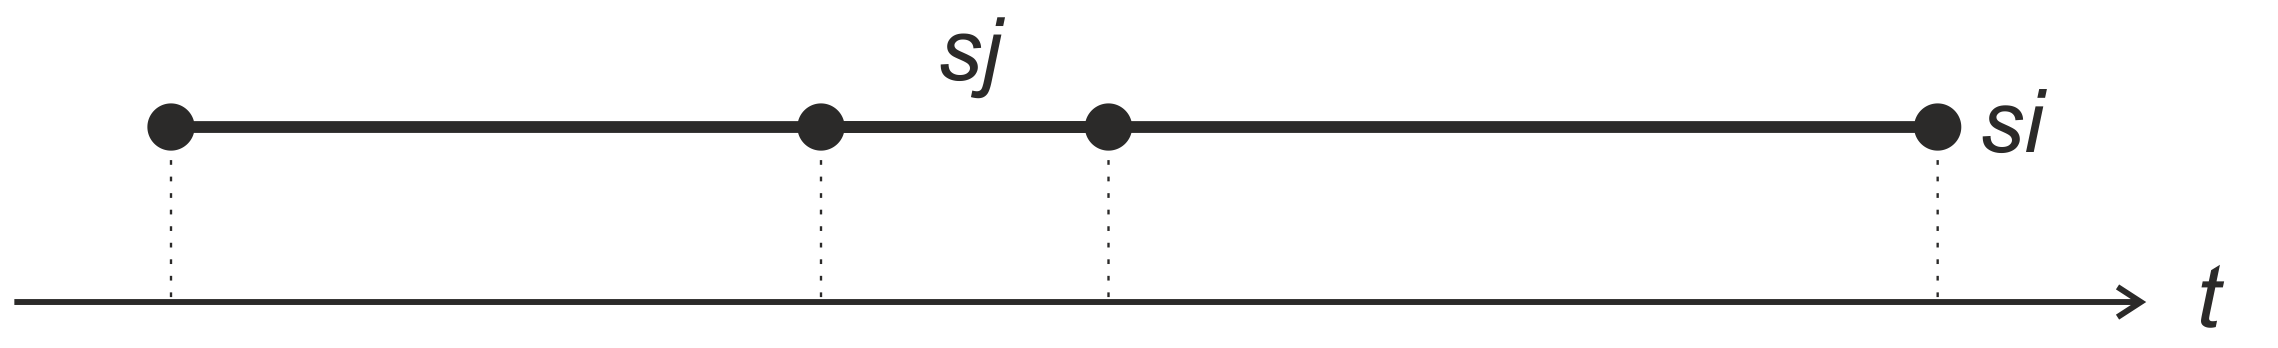
\includegraphics[width=1\linewidth]{figures/sd_temp_entities/img_temporal_part.png}}}
\scntext{примечание}{Связки отношения \textbf{\textit{темпоральная часть*}} связывают две \textit{временные сущности}, одна из которых является частью другой, например, действие и одно из его поддействий. Соответственно, период существования одной из этих сущностей всегда будет включаться в период существования другой (большей).

В отличие от более общего отношения \textit{темпоральное включение*}, связки которого могут связывать любые \textit{временные сущности}, связки отношения \textbf{\textit{темпоральное включение*}} связывают только \textit{временные сущности}, одна из которых является частью другой.}

\scnheader{начальный этап*}

\scnheader{конечный этап*}

\scnheader{промежуточный этап*}

\scnheader{темпоральное включение без совпадения начальных и конечных моментов*}
\scnidtf{строгое темпоральное включение*}
\scnrelfrom{типичная семантическая окрестность}{
\scnfilescg{figures/sd_temp_entities/strict_temporal_inclusion.png}}
\scnrelfrom{иллюстрация}{
\scnfileimage{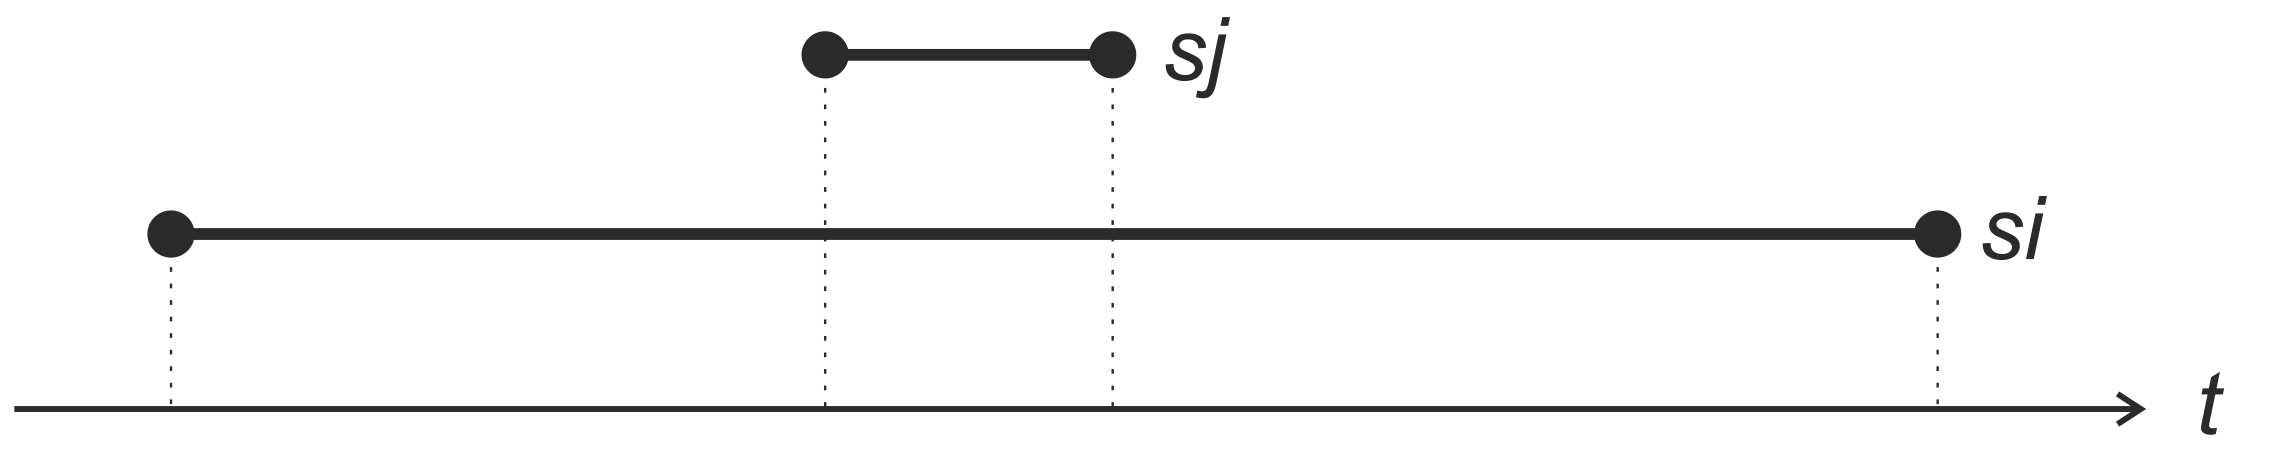
\includegraphics[width=1\linewidth]{figures/sd_temp_entities/img_strict_temporal_inclusion.png}}}
%
% темпоральное включение без совпадения начальных и конечных %моментов
%

\scnheader{темпоральное включение с совпадением начальных моментов*}
\scnrelfrom{типичная семантическая окрестность}{
\scnfilescg{figures/sd_temp_entities/temporal_include_with_match_start_points.png}}
\scnrelfrom{иллюстрация}{
\scnfileimage{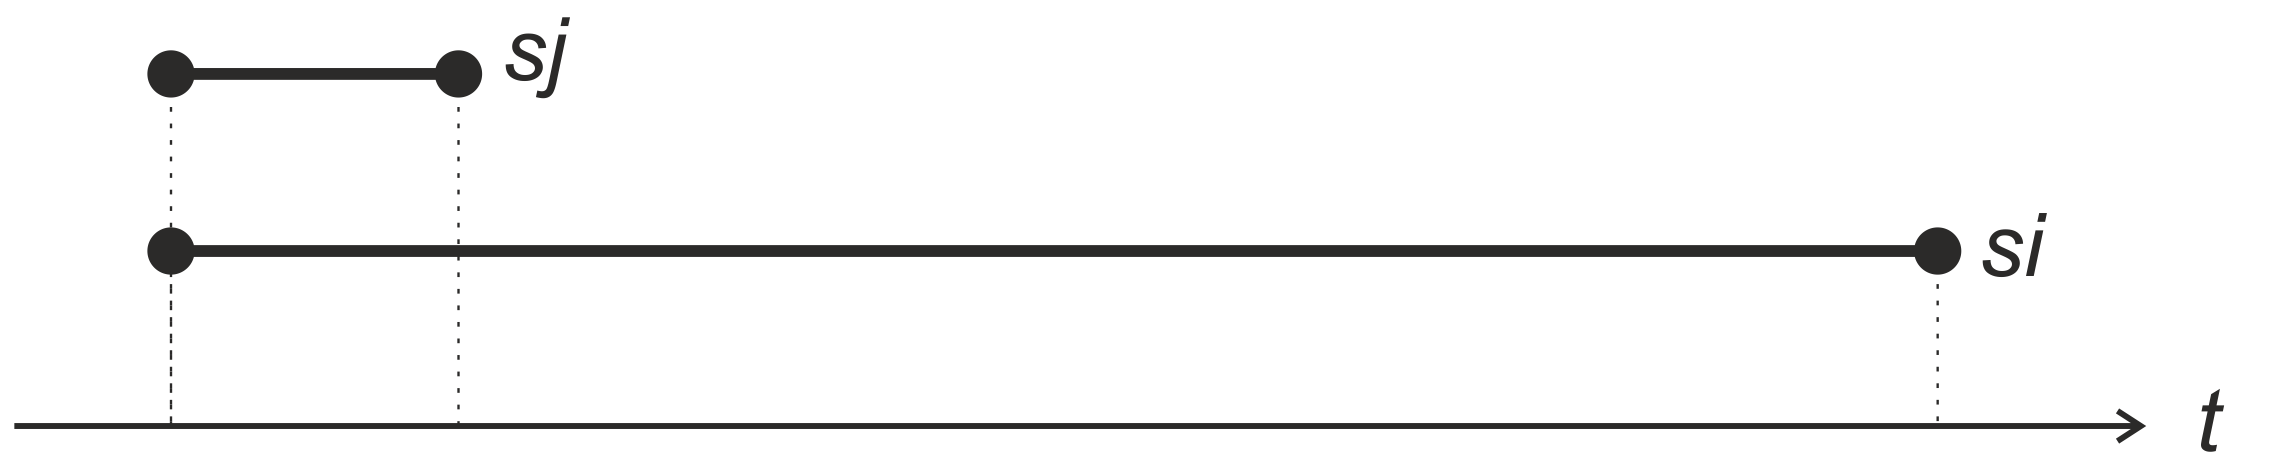
\includegraphics[width=1\linewidth]{figures/sd_temp_entities/img_temporal_include_with_match_start_points.png}}}

\scnheader{темпоральное включение с совпадением конечных моментов*}
\scnrelfrom{типичная семантическая окрестность}{
\scnfilescg{figures/sd_temp_entities/temporal_include_with_terminal_point_match.png}}
\scnrelfrom{иллюстрация}{
\scnfileimage{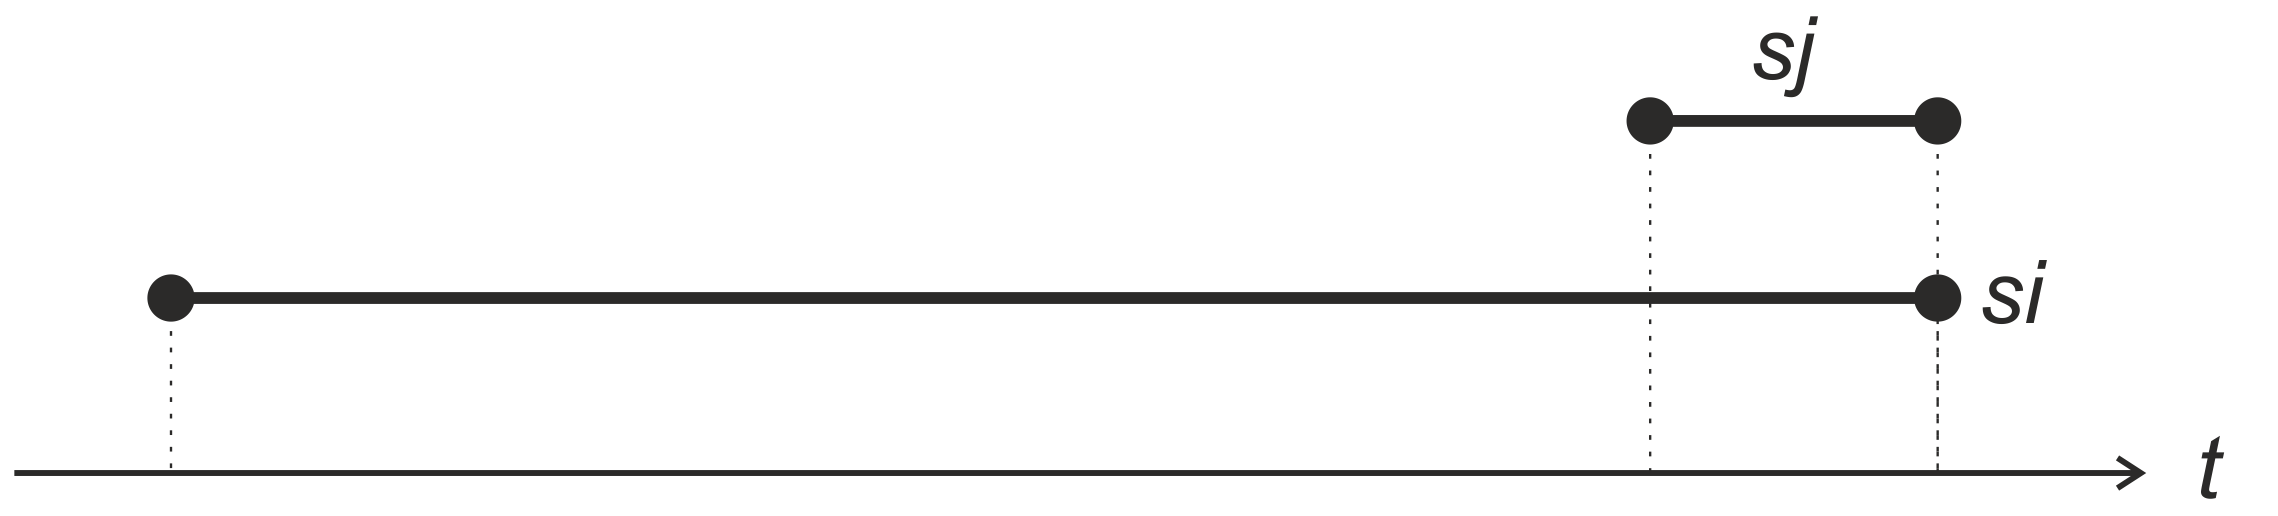
\includegraphics[width=1\linewidth]{figures/sd_temp_entities/img_temporal_include_with_terminal_point_match.png}}}

\scnheader{темпоральное совпадение*}
\scnidtf{совпадение начала и завершения*}

\scnheader{темпоральное объединение*}
\scnrelfrom{типичная семантическая окрестность}{
\scnfilescg{figures/sd_temp_entities/temporal_union.png}}
\scnrelfrom{иллюстрация}{
\scnfileimage{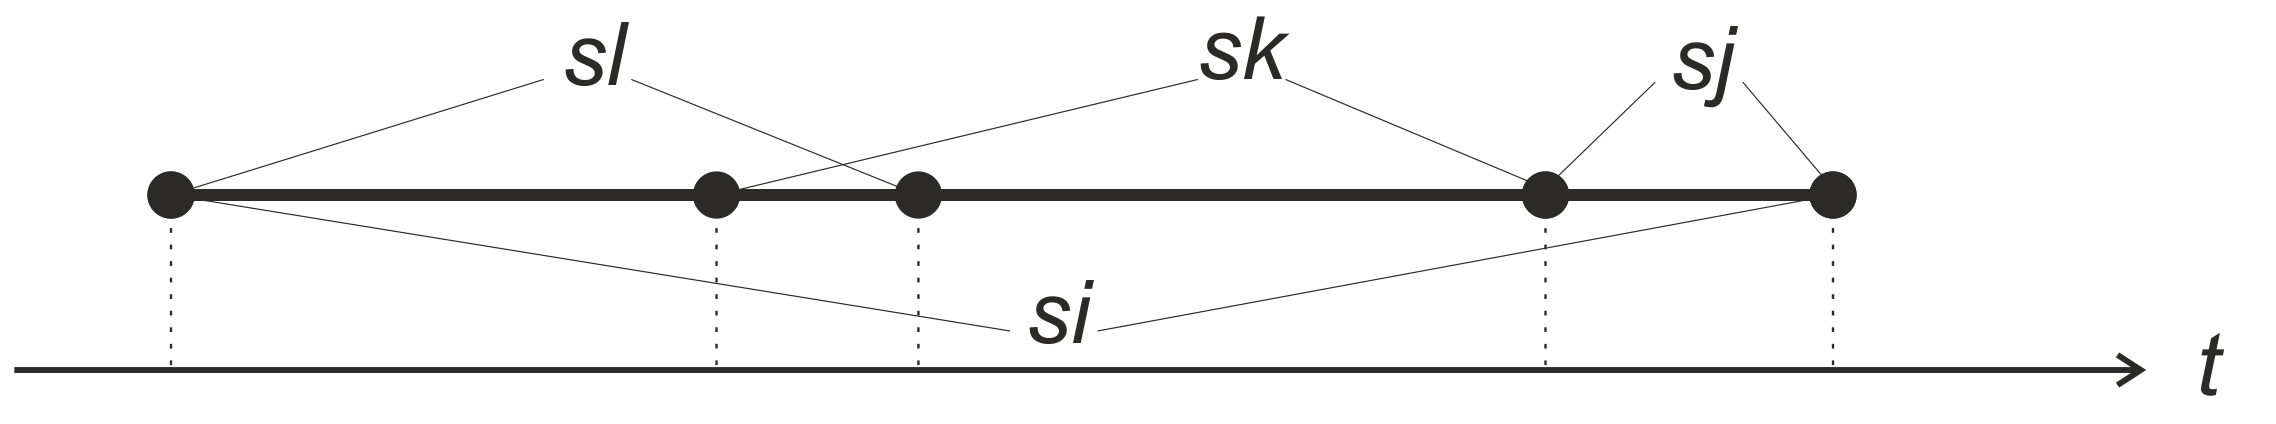
\includegraphics[width=1\linewidth]{figures/sd_temp_entities/img_temporal_union.png}}}

\scnheader{темпоральная декомпозиция*}
\scnrelfrom{типичная семантическая окрестность}{
\scnfilescg{figures/sd_temp_entities/temporal_decomposition.png}}
\scnrelfrom{иллюстрация}{
\scnfileimage{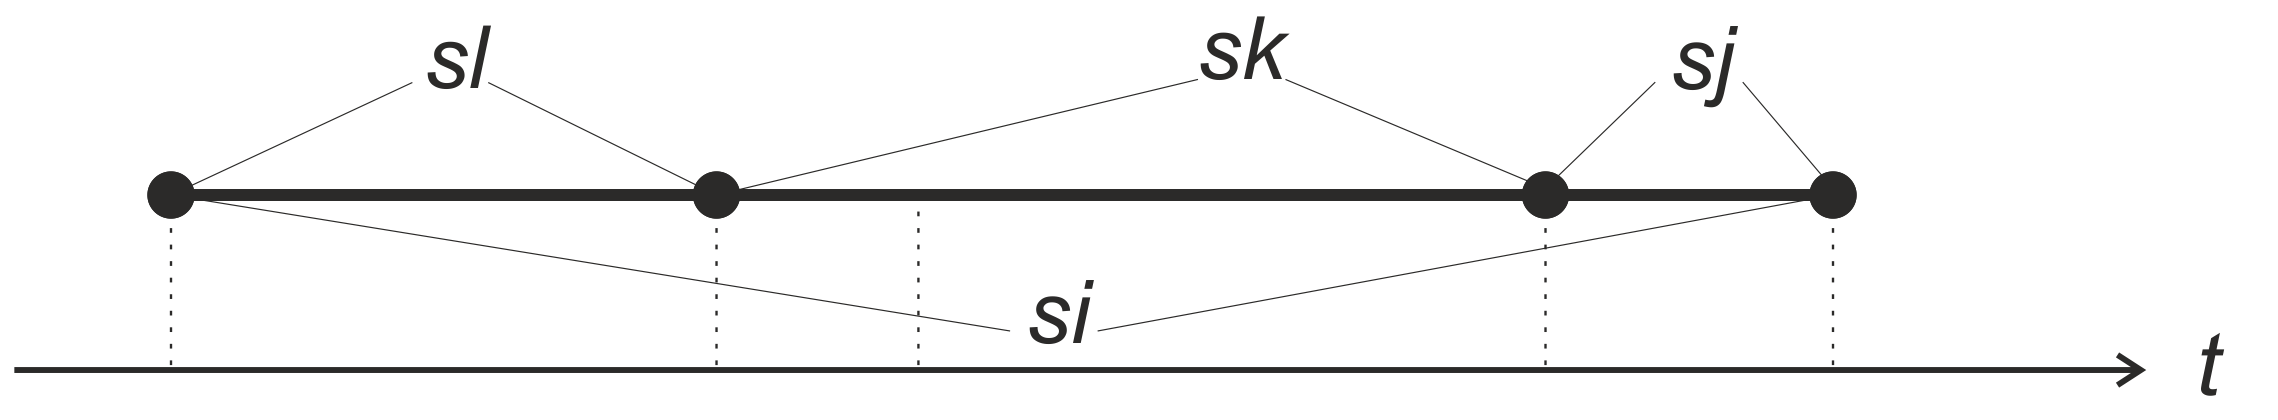
\includegraphics[width=1\linewidth]{figures/sd_temp_entities/img_temporal_decomposition.png}
}}

\scnheader{темпоральная смежность*}
\scnidtf{строгая темпоральная последовательность (без темпорального промежутка)*}
\scnidtf{темпоральная последовательность без промежутка*}
\scnrelfrom{типичная семантическая окрестность}{
\scnfilescg{figures/sd_temp_entities/temporal_adjacency.png}}
\scnrelfrom{иллюстрация}{
\scnfileimage{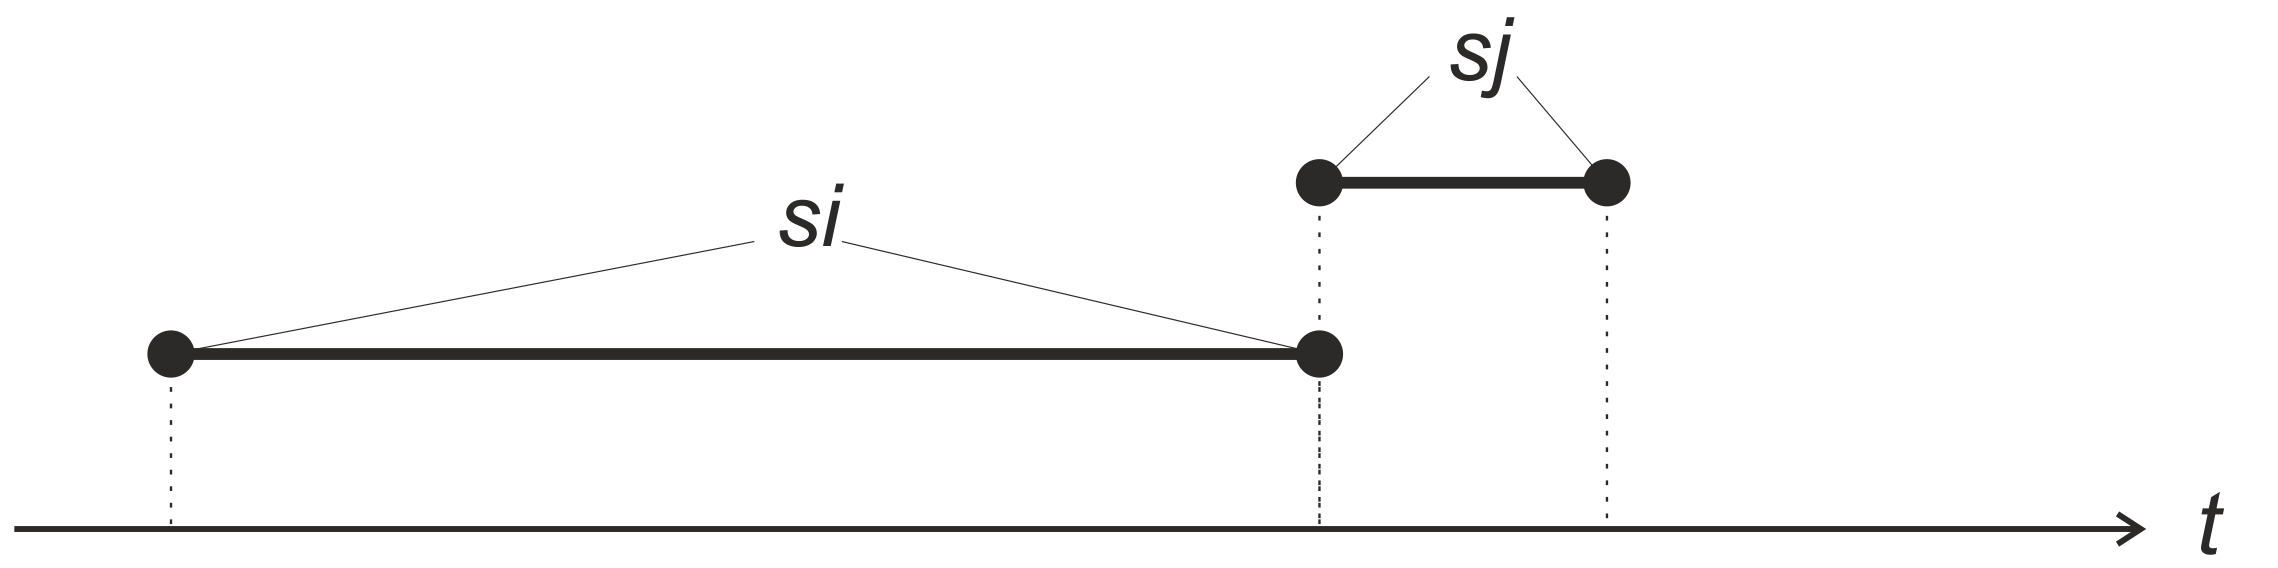
\includegraphics[width=1\linewidth]{figures/sd_temp_entities/img_temporal_adjacency.png}
}}

\scnheader{темпоральная последовательность с промежутком*}
\scnrelfrom{типичная семантическая окрестность}{
\scnfilescg{figures/sd_temp_entities/temporal_sequence_with_intermediate.png}}
\scnrelfrom{иллюстрация}{
\scnfileimage{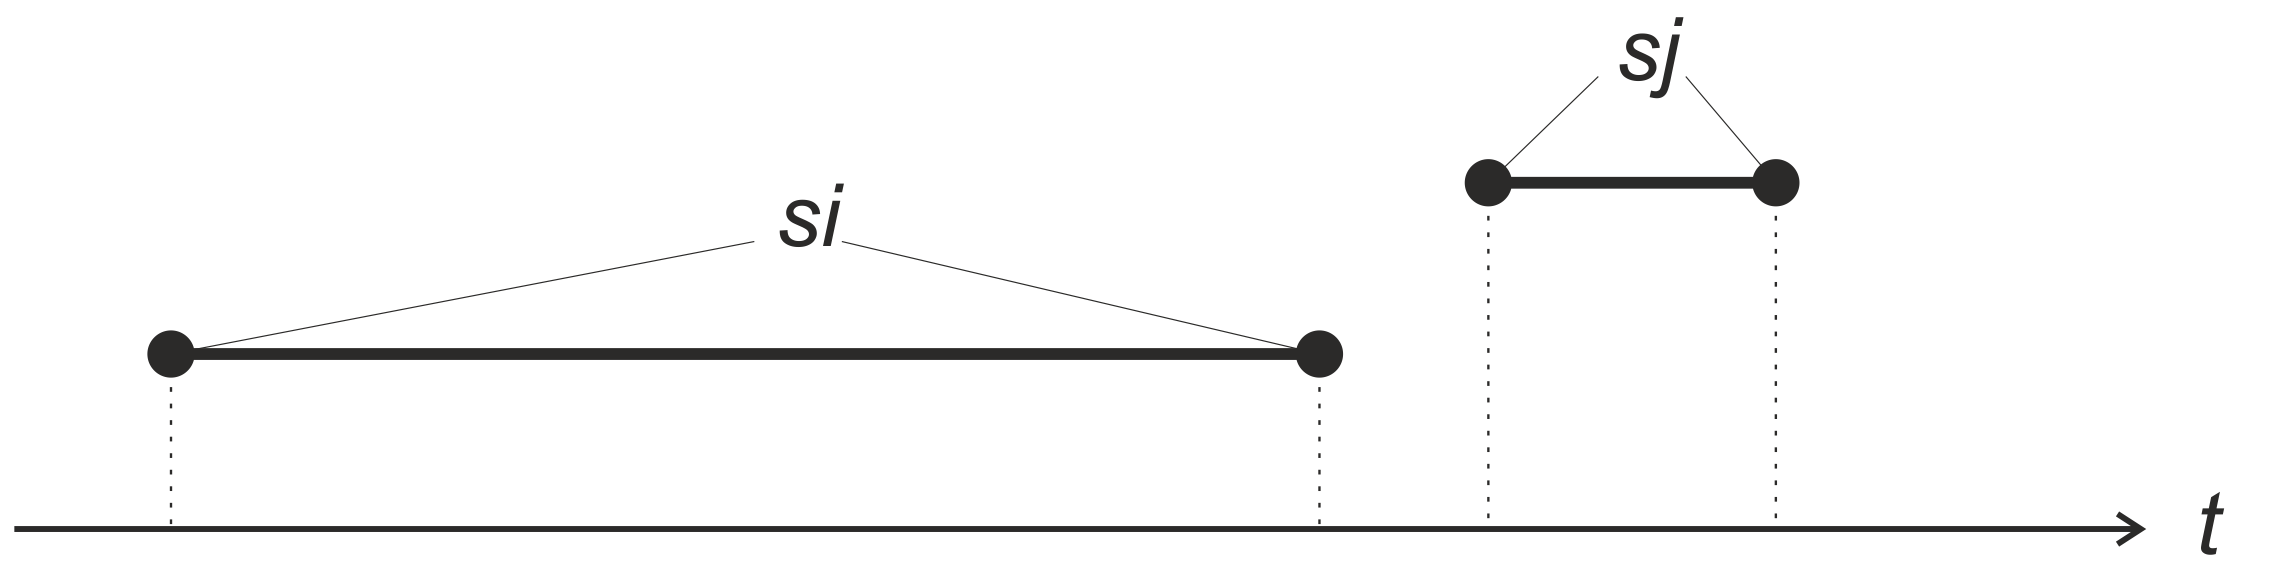
\includegraphics[width=1\linewidth]{figures/sd_temp_entities/img_temporal_sequence_with_intermediate.png}}}

\scnheader{темпоральная последовательность с пересечением*}
\scnrelfrom{типичная семантическая окрестность}{
\scnfilescg{figures/sd_temp_entities/temporal_sequence_with_intersection.png}
}
\scnrelfrom{иллюстрация}{
\scnfileimage{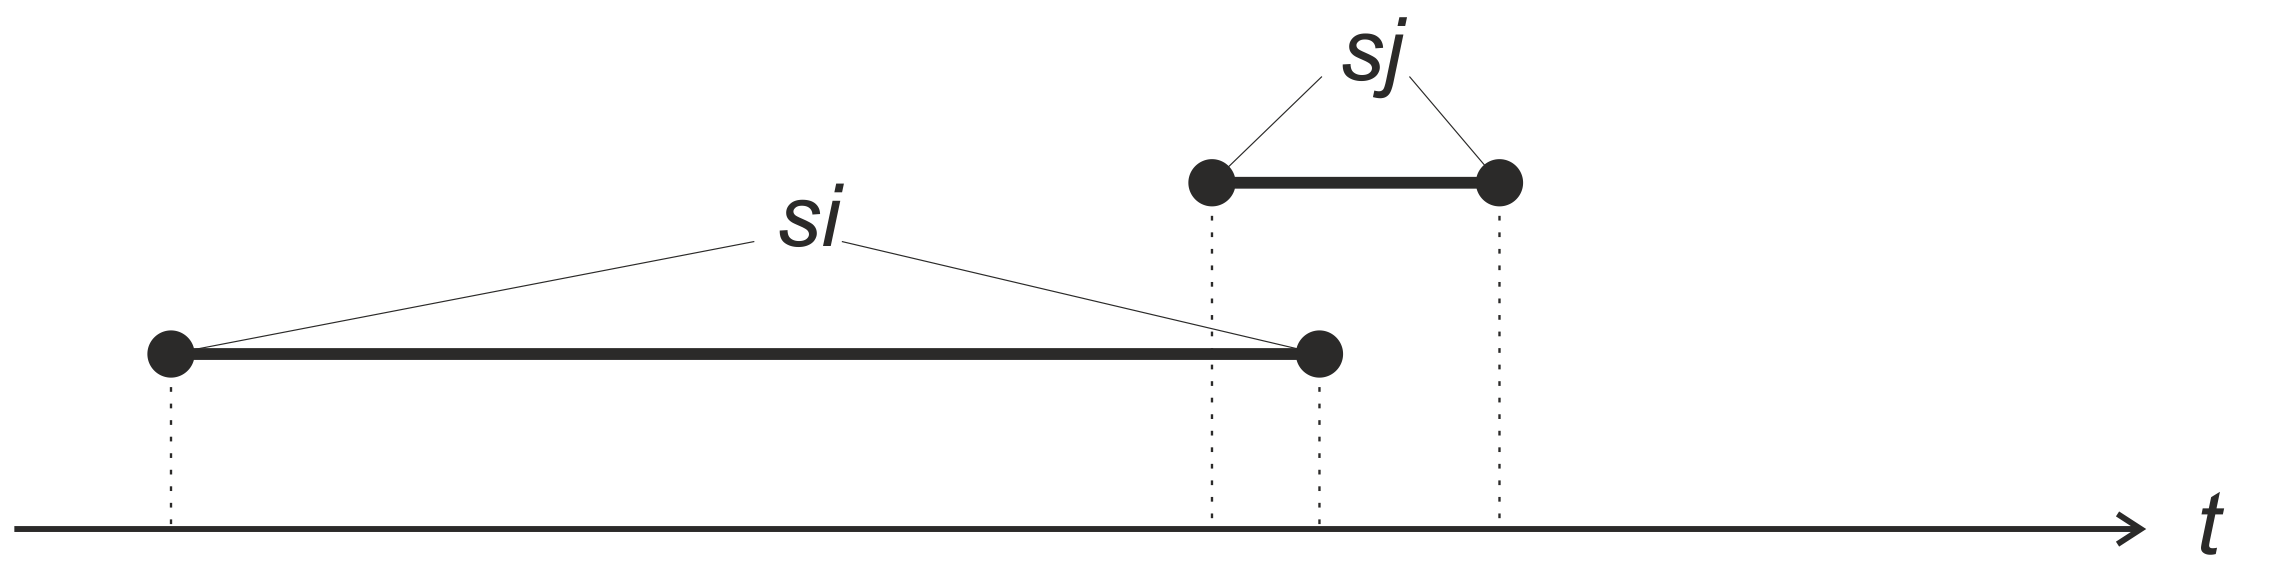
\includegraphics[width=1\linewidth]{figures/sd_temp_entities/img_temporal_cross_sequence.png}
}}

\scnheader{начало}
\scnidtf{класс одновременно начавшихся сущностей}
\scniselement{параметр}
\scnexplanation{Каждый элемент множества \textbf{начало} представляет собой класс \textit{временных сущностей}, у которых совпадает момент начала их существования. Конкретное значение данного \textit{параметра} может быть как \textit{точной величиной}, так и \textit{неточной величиной} или \textit{интервальной величиной}.}
\scnrelfrom{типичная семантическая окрестность}{
\scnfilescg{figures/sd_temp_entities/start.png}}
\scncomment{В данном примере \textbf{\textbf{\textit{ki}}} обозначает класс сущностей, начавших свое существование 19 февраля 2015 года по григорианскому календарю. Конкретные примеры таких сущностей – \textbf{\textit{bi}} и \textbf{\textit{bj}}. \textbf{\textit{ti}} обозначает временную точку григорианского календаря, соответствующую 19 февраля 2015 года.}

\scnheader{завершение}
\scnidtf{конец}
\scnidtf{класс одновременно завершившихся сущностей}
\scniselement{параметр}
\scnexplanation{Каждый элемент множества \textbf{\textit{завершение}} представляет собой класс \textit{временных сущностей}, у которых совпадает конечный момент их существования (момент завершения существования). Конкретное значение данного \textit{параметра} может быть как \textit{точной величиной}, так и \textit{неточной величиной} или \textit{интервальной величиной}.}
\scnrelfrom{типичная семантическая окрестность}{
\scnfilescg{figures/sd_temp_entities/completion.png}}
\scncomment{В данном примере \textbf{\textit{ki}} обозначает класс сущностей, завершивших свое существование 21 февраля 2015 года по григорианскому календарю. Конкретные примеры таких сущностей – \textbf{\textit{bi}} и \textbf{\textit{bj}}. \textbf{\textit{ti}} обозначает временную точку григорианского календаря, соответствующую 21 февраля 2015 года.}

\scnheader{длительность}
\scnidtf{класс временных сущностей, имеющих одинаковую длительность}
\scniselement{параметр}
\scnhaselement{тысячелетие}
\scnhaselement{век}
\scnhaselement{год}
\scnhaselement{месяц}
\scnhaselement{день}
\scnhaselement{час}
\scnhaselement{минута}
\scnhaselement{секунда}
\scnexplanation{Каждый элемент множества \textbf{\textit{длительность}} представляет собой класс \textit{временных сущностей}, у которых совпадает длительность их существования. Конкретное значение данного \textit{параметра} может быть как \textit{точной величиной}, так и \textit{неточной величиной} или \textit{интервальной величиной}.}
\scnrelfrom{типичная семантическая окрестность}{
\scnfilescg{figures/sd_temp_entities/duration.png}}
\scncomment{В данном примере \textbf{\textit{ki}} обозначает класс сущностей, существовавших в течение 2 месяцев. Конкретный пример такой сущности – \textbf{\textit{bi}}.}

\scnheader{тысячелетие}

\scnheader{век}

\scnheader{год}

\scnheader{месяц}

\scnheader{сутки}

\scnheader{час}

\scnheader{минута}

\scnheader{секунда}

\scnheader{номер тысячелетия\scnrolesign}
\scnheader{номер века\scnrolesign}
\scnheader{номер года\scnrolesign}
\scnheader{номер месяца в году\scnrolesign}
\scnheader{номер суток в месяце\scnrolesign}
\scnheader{номер часа в дне\scnrolesign}
\scnheader{номер минуты в часе\scnrolesign}
\scnheader{номер секунды в минуте\scnrolesign}

\scnendstruct \scnendcurrentsectioncomment

\end{SCn}

\scsection{Предметная область и онтология темпоральных сущностей баз знаний ostis-систем}
\begin{SCn}

\scnsectionheader{\currentname}
\scntext{введение}{Обработка информации в \textit{sc-памяти} (т.е. динамика базы знаний, хранимой в \textit{sc-памяти}) в конечном счете сводится:
\begin{scnitemize}
    \item к появлению в \textit{sc-памяти} новых актуальных \textit{sc-узлов} и \textit{sc-коннекторов};
    \item к логическому удалению актуальных \textit{sc-элементов}, т.е. к переводу их в неактуальное состояние (это необходимо для хранения протокола изменения состояния базы знаний, в рамках которого могут описываться действия по удалению \textit{sc-элементов});
    \item к возврату логически удаленных \textit{sс-элементов} в статус актуальных (необходимость в этом может возникнуть при откате базы знаний к какой-нибудь ее прошлой версии);
    \item к физическому удалению \textit{sc-элементов};
    \item к изменению состояния актуальных (логически не удаленных \textit{sc-элементов}) – \textit{sc-узел} может превратиться в \textit{sc-ребро}, \textit{sc-ребро} может превратиться в \textit{sc-дугу}, \textit{sc-дуга} может поменять направленность, \textit{sc-дуга} общего вида может превратиться в \textit{константную стационарную sc-дугу принадлежности}, и т.д.;
\end{scnitemize}
Подчеркнем, что временный характер самого \textit{sc-элемента} (т.к. он может появиться или исчезнуть) никак не связан с возможно временным характером сущности, обозначаемой этим \textit{sc-элементом}. Т.е. временный характер самого sc-элемента и временный характер сущности, которую он обозначает – абсолютно разные вещи.

Таким образом, следует четко отличать динамику внешнего мира, описываемого базой знаний, а динамику самой базы знаний (динамику внутреннего мира). При этом очень важно, чтобы описание динамики базы знаний также входило в состав каждой базы знаний.

К числу понятий, используемых для описания динамики базы знаний относятся:
\begin{scnitemize}
    \item логически удаленный sc-элемент;
    \item сформированное множество;
    \item вычисленное число;
    \item сформированное высказывание;
\end{scnitemize}}

\scnstartsubstruct

\scnheader{Предметная область темпоральных сущностей базы знаний ostis-системы}
\scnidtf{Предметная область, описывающая динамику базы знаний, хранимой в sc-памяти}
\scniselement{предметная область}
\scnsdmainclasssingle{ситуация}
\scnsdclass{sc-элемент;наcтоящий sc-элемент;логически удаленный sc-элемент;число;невычисленное число;вычисленное число;понятие;основное понятие;неосновное понятие;понятие, переходящее из основного в неосновное;понятие, переходящее из неосновного в основное;специфицированная сущность;недостаточно специфицированная сущность;достаточно специфицированная сущность;средне специфицированная сущность;структура;файл;событие в sc-памяти*;элементарное событие в sc-памяти*;событие добавления sc-дуги, выходящей из заданного sc-элемента*;событие добавления sc-дуги, входящей в заданный sc-элемент*;событие добавления sc-ребра, инцидентного заданному sc-элементу*;событие удаления sc-дуги, выходящей из заданного sc-элемента*;событие удаления sc-дуги, входящей в заданный sc-элемент*;событие удаления sc-ребра, инцидентного заданному sc-элементу*;событие удаления sc-элемента*;событие изменения содержимого файла*}

\scnheader{sc-элемент}
\scnreltoset{разбиение}{наcтоящий sc-элемент;логически удаленный sc-элемент}

\scnheader{наcтоящий sc-элемент}
\scniselement{ситуативное множество}

\scnheader{логически удаленный sc-элемент}
\scniselement{ситуативное множество}

\scnheader{число}
\scnsubdividing{невычисленное число;вычисленное число}

\scnheader{невычисленное число}
\scniselement{ситуативное множество}

\scnheader{вычисленное число}

\scnheader{понятие}
\scnsubdividing{основное понятие;неосновное понятие;понятие, переходящее из основного в неосновное;понятие, переходящее из неосновного в основное}

\scnheader{основное понятие}
\scnidtf{основное понятие для данной ostis-системы}
\scniselement{ситуативное множество}
\scnexplanation{К \textbf{\textit{основным понятиям}} относятся те понятия, которые активно используются в системе и могут быть ключевыми элементами sc-агентов. К \textbf{\textit{основным понятиям}} относятся также все неопределяемые понятия.}

\scnheader{неосновное понятие}
\scnidtf{дополнительное понятие}
\scnidtf{вспомогательное понятие}
\scnidtf{неосновное понятие для данной ostis-системы}
\scniselement{ситуативное множество}
\scnexplanation{Каждое \textbf{\textit{неосновное понятие}} должно быть строго определено на основе \textit{основных понятий}. Такие \textbf{\textit{неосновные понятия}} используются только для понимания и правильного восприятия вводимой информации, в том числе, для выравнивания онтологий. Ключевым элементом \textit{sc-агентов} \textbf{\textit{неосновные понятия}} быть не могут.}
\scntext{правило идентификации экземпляров}{В случае, когда некоторое понятие полностью перешло из \textit{основных понятий} в неосновные, то есть стало \textbf{\textit{неосновным понятием}}, и соответствующее ему \textit{основное понятие} (через которое оно определяется) в рамках некоторого внешнего языка имеет одинаковый с ним основной идентификатор, то к идентификатору \textbf{\textit{неосновного понятия}} спереди добавляется знак \#. Если при этом соответствуюшее \textit{основное понятие} имеет в идентификаторе знак \$, добавленный в процессе перехода, то этот знак удаляется. Если указанные понятия имеют разные основные идентификаторы в рамках этого внешнего языка, то никаких дополнительных средств идентификации не используется.

Например:\\
\textit{\#трансляция sc-текста}\\
\textit{\#scp-программа}}

\scnheader{понятие, переходящее из основного в неосновное}
\scniselement{ситуативное множество}

\scnheader{понятие, переходящее из неосновного в основное}
\scniselement{ситуативное множество}
\scntext{правило идентификации экземпляров}{В случае, когда текущее \textit{основное понятие} и соответствующее ему \textbf{\textit{понятие, переходящее из неосновного в основное}} в рамках некоторого внешнего языка имеют одинаковый основной идентификатор, то к идентификатору понятия, переходящего из неосновного в основное спереди добавляется знак \$. Если указанные понятия имеют разные основные идентификаторы в рамках этого внешнего языка, то никаких дополнительных средств идентификации не используется.

Например:\\
\textit{\$трансляция sc-текста}\\
\textit{\$scp-программа}}

\scnheader{специфицированная сущность}
\scnsubdividing{недостаточно специфицированная сущность;достаточно специфицированная сущность;средне специфицированная сущность}

\scnheader{недостаточно специфицированная сущность}

\scnheader{достаточно специфицированная сущность}
\scnexplanation{К \textbf{\textit{достаточно специфицированным сущностям}} предъявляются следующие требования:
\begin{scnitemize}
    \item если сущность не является понятием, то для нее должны быть указаны
    \begin{scnenumerate}
    \item различные варианты обозначающих ее внешних знаков;
    \item классы, которым она принадлежит;
    \item связки, которыми она связана с другими сущностями (с указанием соответствующего отношения);
    \item значения параметров, которыми она обладает;
    \item те разделы базы знаний, в которых указанная сущность является ключевой;
    \item предметные области, в которые данная сущность входит.
    \end{scnenumerate}
    \item если специфицированная сущность является понятием, то для нее должны быть указаны:
    \begin{scnenumerate}
    \item различные варианты внешних обозначений этого понятия;
    \item предметные области, в которых это понятие исследуется;
    \item определение понятия;
    \item пояснения
    \item разделы базы знаний, в которых это понятие является ключевым;
    \item типичная семантическая окрестность – пример экземпляра понятия.
    \end{scnenumerate}
\end{scnitemize}}

\scnheader{средне специфицированная сущность}

\scnheader{структура}
\scnsubdividing{сформированная структура;несформированная структура}
\scnsubdividing{недостаточно сформированная структура;достаточно сформированная структура;структура, имеющая средний уровень сформированности}

\scnheader{файл}
\scnsubdividing{недостаточно сформированный внутренний файл;достаточно сформированный внутренний файл;внутренний файл, имеющий средний уровень сформированности}

\scnheader{событие в sc-памяти*}
\scnrelto{включение}{событие*}

\scnheader{элементарное событие в sc-памяти*}
\scnrelto{включение}{событие в sc-памяти*}
\scnexplanation{Под \textbf{\textit{элементарным событием в sc-памяти*}} понимается \textit{событие*}, соответствующее некоторому действию в \textit{sc-памяти}, в результате выполнения которого изменяется состояние только одного \textit{sc-элемента}.}
\scnsubdividing{событие добавления sc-дуги, выходящей из заданного sc-элемента*
;событие добавления sc-дуги, входящей в заданный sc-элемент*;событие добавления sc-ребра, инцидентного заданному sc-элементу*;событие удаления sc-дуги, выходящей из заданного sc-элемента*;событие удаления sc-дуги, входящей в заданный sc-элемент*;событие удаления sc-ребра, инцидентного заданному sc-элементу*;событие удаления sc-элемента*;событие изменения содержимого файла*}

\scnheader{событие добавления sc-дуги, выходящей из заданного sc-элемента*}

\scnheader{событие добавления sc-дуги, входящей в заданный sc-элемент*}

\scnheader{событие добавления sc-ребра, инцидентного заданному sc-элементу*}

\scnheader{событие удаления sc-дуги, выходящей из заданного sc-элемента*}

\scnheader{событие удаления sc-дуги, входящей в заданный sc-элемент*}

\scnheader{событие удаления sc-ребра, инцидентного заданному sc-элементу*}

\scnheader{событие удаления sc-элемента*}

\scnheader{событие изменения содержимого файла*}

\scnendstruct

\end{SCn}

\scsection{Предметная область и онтология семантических окрестностей}
\label{sec:sd_sem_neigh}
\begin{SCn}

\scnsectionheader{\currentname}

\scnstartsubstruct

\scnheader{Предметная область семантических окрестностей}
\scniselement{предметная область}
\scnsdmainclasssingle{семантическая окрестность}
\scnsdclass{семантическая окрестность по инцидентным коннекторам;семантическая окрестность по выходящим дугам;семантическая окрестность по выходящим дугам принадлежности;семантическая окрестность по входящим дугам;семантическая окрестность по входящим дугам принадлежности;полная семантическая окрестность;базовая семантическая окрестность;специализированная семантическая окрестность;пояснение;примечание;правило идентификации экземпляров;терминологическая семантическая окрестность;теоретико-множественная семантическая окрестность;описание декомпозиции;логическая семантическая окрестность;спецификация типичного экземпляра;сравнительный анализ}

\scnheader{семантическая окрестность}
\scnidtf{sc-окрестность}
\scnidtf{семантическая окрестность, представленная в виде sc-текста}
\scnidtf{sc-текст, являющийся семантической окрестностью некоторого sc-элемента}
\scnidtf{спецификация заданной сущности, знак которой указывается как ключевой элемент этой спецификации}
\scnidtf{описание заданной сущности, знак которой указывается как ключевой элемент этой спецификации}
\scnsubset{знание}
\scnsuperset{семантическая окрестность по инцидентным коннекторам}
\scnsuperset{полная семантическая окрестность}
\scnsuperset{базовая семантическая окрестность}
\scnsuperset{специализированная семантическая окрестность}
\scnidtftext{пояснение}{\textit{знание}, являющееся спецификацией (описанием) некоторой \textit{сущности}, знак которой является \textit{ключевым знаком\scnrolesign} указанного \textit{знания}. Заметим, что каждая \textit{семантическая окрестность} в отличие от \textit{знаний} других видов имеет только один \textit{ключевой знак\scnrolesign} (ключевой элемент\scnrolesign, знак описываемой сущности\scnrolesign). Заметим также, что многообразие видов семантических окрестностей свидетельствует о многообразии семантических видов описаний различных сущностей.}
\scnnote{Понятие \textit{семантической окрестности}, как и любой другой \uline{семантически} выделяемый класс \textit{знаний}, абсолютно не зависит от \textit{языка представления знаний}. Этим \textit{языком} может быть не только \textit{SC-код} или другой \textit{формальный язык представления знаний} или даже \textit{естественный язык}, тексты которых в \textit{памяти ostis-системы} представляются в виде \textit{файлов}.}

\scnheader{семантическая окрестность по инцидентным коннекторам}
\scnsuperset{семантическая окрестность по выходящим дугам}
\scnsuperset{семантическая окрестность по входящим дугам}
\scnidtftext{пояснение}{вид \textit{семантической окрестности}, в которую входят все коннекторы, инцидентные заданному элементу, а также все элементы, инцидентные указанным коннекторам.}

\scnheader{семантическая окрестность по выходящим дугам}
\scnsuperset{семантическая окрестность по выходящим дугам принадлежности}
\scnidtftext{пояснение}{вид \textit{семантической окрестности}, в которую входят все дуги, выходящие из заданного sc-элемента и вторые компоненты этих дуг. Также указывается факт принадлежности этих дуг каким-либо отношениям.}

\scnheader{семантическая окрестность по выходящим дугам принадлежности}
\scnidtftext{пояснение}{вид \textit{семантической окрестности}, в которую входят все дуги принадлежности, выходящие из заданного \textit{sc-элемента}, а также их вторые компоненты. При необходимости может указывается факт \textit{принадлежности} этих дуг каким-либо \textit{ролевым отношениям}.}

\scnheader{семантическая окрестность по входящим дугам}
\scnsuperset{семантическая окрестность по входящим дугам принадлежности}
\scnidtftext{пояснение}{вид \textit{семантической окрестности}, в которую входят все дуги, входящие в заданный sc-элемент, а также их первые компоненты. Также указывается факт принадлежности этих дуг каким-либо отношениям.}

\scnheader{семантическая окрестность по входящим дугам принадлежности}
\scnidtftext{пояснение}{вид \textit{семантической окрестности}, в которую входят все дуги принадлежности, входящие в заданный sc-элемент, а также их первые компоненты. При необходимости может указывается факт принадлежности этих дуг каким-либо ролевым отношениям.}

\scnheader{полная семантическая окрестность}
\scnidtf{полная спецификация некоторой описываемой сущности}
\scnidtftext{пояснение}{вид \textit{семантической окрестности}, включающий описание всех связей описываемой сущности. 

Структура полной семантической окрестности определяется прежде всего семантической типологией описываемой сущности. 

Так, например, для \textit{понятия} в \textit{полную семантическую окрестность} необходимо включить следующую информацию (при наличии):
\begin{scnitemize}
    \item варианты идентификации на различных внешних языках (sc-идентификаторы);
    \item принадлежность некоторой \textit{предметной области} с указанием роли, выполняемой в рамках этой предметной области;
    \item теоретико-множественные связи заданного \textit{понятия} с другими \textit{sc-элементами};
    \item определение или пояснение;
    \item высказывания, описывающие свойства указанного \textit{понятия};
    \item задачи и их классы, в которых данное \textit{понятие} является ключевым;
    \item описание типичного примера использования указанного \textit{понятия};
    \item экземпляры описываемого \textit{понятия}.
\end{scnitemize}
Для понятия, являющегося отношением дополнительно указываются:
\begin{scnitemize}
    \item домены;
    \item область определения;
    \item схема отношения;
    \item классы отношений, которым принадлежит описываемое отношение.
\end{scnitemize}
}

\scnheader{базовая семантическая окрестность}
\scnidtf{минимально достаточная семантическая окрестность}
\scnidtf{минимальная спецификация описываемой сущности}
\scnidtf{сокращенная спецификация описываемой сущности}
\scnidtf{основная семантическая окрестность}
\scnidtftext{пояснение}{вид \textit{семантической окрестности}, содержащий минимальную (краткую) информацию об описываемой сущности

Структура базовой семантической окрестности определяется прежде всего семантической типологией описываемой сущности. 

Так, например, для \textit{понятия} в базовую семантическую окрестность необходимо включить следующую информацию (при наличии): 
\begin{scnitemize}
    \item варианты идентификации на различных внешних языках (sc-идентификаторы);
    \item принадлежность некоторой \textit{предметной области} с указанием роли, выполняемой в рамках этой предметной области;
    \item \textit{определение} или пояснение.
\end{scnitemize}
Для \textit{понятия}, являющегося \textit{отношением} дополнительно указываются:
\begin{scnitemize}
    \item \textit{домены};
    \item \textit{область определения};
    \item описание типичного примера связки указанного отношения (спецификация типичного экземпляра).
\end{scnitemize}
}

\scnheader{специализированная семантическая окрестность}
\scnsuperset{пояснение}
\scnsuperset{примечание}
\scnsuperset{правило идентификации экземпляров}
\scnsuperset{терминологическая семантическая окрестность}
\scnsuperset{теоретико-множественная семантическая окрестность}
\scnsuperset{логическая семантическая окрестность}
\scnsuperset{описание типичного экземпляра}
\scnsuperset{описание декомпозиции} 
\scnidtftext{пояснение}{вид \textit{семантической окрестности}, набор связей для которой уточняется отдельно для каждого типа такой окрестности.}

\scnheader{пояснение}
\scnidtf{sc-пояснение}
\scnidtftext{пояснение}{знак sc-текста, поясняющего описываемую сущность.}

\scnheader{примечание}
\scnidtf{sc-примечание}
\scnidtftext{пояснение}{знак sc-текста, являющегося примечанием к описываемой сущности. В примечании обычно описываются особые свойства и исключения из правил для описываемой сущности.}

\scnheader{правило идентификации экземпляров}
\scnidtf{правило идентификации экземпляров заданного класса}
\scnidtftext{пояснение}{sc-текст являющийся описанием правил построения идентификаторов элементов заданного класса.}

\scnheader{терминологическая семантическая окрестность}
\scnidtftext{пояснение}{\textit{семантическая окрестность}, описывающая внешнюю идентификацию указанной сущности, т.е. её sc-идентификаторы}

\scnheader{теоретико-множественная семантическая окрестность}
\scnidtftext{пояснение}{описание связи описываемого множества с другими множествами с помощью теоретико-множественных отношений}

\scnheader{описание декомпозиции}
\scnidtf{\textit{семантическая окрестность}, описывающая декомпозицию некоторой сущности}
\scnidtftext{пояснение}{\textit{семантическая окрестность}, описывающая декомпозицию некоторой сущности на её части}

\scnheader{логическая семантическая окрестность }
\scnidtftext{пояснение}{\textit{семантическая окрестность}, описывающая семейство высказываний, описывающих свойства данного \textit{понятия} или какого-либо конкретного экземпляра некоторого понятия}

\scnheader{спецификация типичного экземпляра}
\scnidtf{описание типичного экземпляра заданного класса}
\scnidtftext{пояснение}{sc-текст являющийся описанием типичного примера рассматриваемого класса.}

\scnheader{сравнительный анализ}
\scnidtftext{пояснение}{описание сравнения некоторой сущности с другими аналогичными сущностями}

\scnheader{сравнение}
\scnidtftext{пояснение}{описание сравнения (сходств и отличий) двух сущностей, которые заданы \textit{парой} (двухмощными множествами), которому принадлежат знаки обеих сравниваемых сущностей}

\scnheader{семантическая окрестность}
\scnnote{Всему классу \textit{семантических окрестностей} и всем подклассам этого \textit{класса}, а так же всем другим классам \textit{знаний}, ставятся в соответствие \textit{бинарные ориентированые отношения}, вторыми \textit{доменами} которых являются указанные \textit{классы} и объединение которых является \textit{обратным отношением} для \textit{отношения} "быть ключевым знаком\scnrolesign"{}. Эти отношения не следует причислять к основным отношениям, т.к. они вместе с выделенными классами семантических окрестностей привносят дополнительную логическую эквивалентность в базу знаний.}

\scnheader{семантическая окрестность}
\scnrelfromlist{отношение, заданное на}{семантическая окрестность*
	;семантическая окрестность по инцидентным коннекторам*
	;полная семантическая окрестность*
	;базовая семантическая окрестность*
	;специализированная синтетическая окрестность*
	;и т.д.
}
\scnnote{Понятие семантической окрестности, дополненное уточнением таких понятий, как семантическое расстояние между знаками (семантическая близость знаков), радиус семантической окрестности, является перспективной основой для исследования свойств смыслового пространства.}
\scnendstruct \scnendcurrentsectioncomment

\end{SCn}

\scsection{Предметная область и онтология предметных областей}
\label{sec:sd_sd}
\begin{SCn}

\scnsectionheader{\currentname}

\scnstartsubstruct

\scnheader{Предметная область предметных областей}
\scnidtf{Предметная область, объектами исследования которой являются предметные области}
\scnexplanation{В состав \textbf{\textit{Предметной области предметных областей}} входят структурные спецификации всех \textit{предметных областей}, входящих в состав базы знаний \textit{ostis-системы}, в том числе, самой \textbf{\textit{Предметной области предметных областей}}. Таким образом, \textbf{\textit{Предметная область предметных областей}} является, во-первых, \textit{рефлексивным множеством}, во-вторых, рефлексивной предметной областью, то есть \textit{предметной областью}, одним из объектов исследования которой является она сама.}
\scniselement{рефлексивное множество}
\scnsdmainclasssingle{предметная область}

\scnsdclass{стационарная предметная область;нестационарная предметная область;понятие;sc-язык}

\scnsdrelation{понятие предметной области’;исследуемое понятие’;максимальный класс объектов исследования’;немаксимальный класс объектов исследования’;исследуемый класс первичных элементов’;исследуемое отношение’;класс исследуемых структур';понятие, исследуемое в предметной подобласти’;понятие, исследуемое в более общей предметной области’;понятие, исследуемое в неродственной предметной области’;частная предметная область*;частная предметная область по классу первичных элементов*;частная предметная область по исследуемым отношениям*;неродственные предметные области*;sc-язык и соответствующая предметная область*}

\scnheader{предметная область}
\scnidtf{sc-модель предметной области}
\scnidtf{sc-текст предметной области}
\scnidtf{sc-граф предметной области}
\scnidtf{представление предметной области в SC-коде}
\scnsubset{знание}
\scnsubset{бесконечное множество}
\scnexplanation{\textbf{\textit{Предметная область}} – это результат интеграции (объединения) частичных семантических окрестностей, описывающих все исследуемые сущности заданного класса и имеющих одинаковый (общий) предмет исследования (то есть один и тот же набор отношений, которым должны принадлежать связки, входящие в состав интегрируемых семантических окрестностей).


\textbf{\textit{Предметная область}} – \textit{структура}, в состав которой входят:
\begin{scnenumerate}
\item \textnormal{основные исследуемые (описываемые) объекты – первичные и вторичные;}
\item \textnormal{различные классы исследуемых объектов;}
\item \textnormal{различные связки, компонентами которых являются исследуемые объекты (как первичные, так и вторичные), а также, возможно, другие такие связки – то есть связки (как и объекты исследования) могут иметь различный структурный уровень;}
\item \textnormal{различные классы указанных выше связок (то есть отношения);}
\item \textnormal{различные классы объектов, не являющихся ни объектами исследования, ни указанными выше связками, но являющихся компонентами этих связок.}
\end{scnenumerate}


При этом все классы, объявленные исследуемыми понятиями, должны быть полностью представлены в рамках данной предметной области вместе со своими элементами, элементами элементов и т.д. вплоть до терминальных элементов.


Можно говорить о типологии \textbf{\textit{предметных областей}} по разным структурным признакам:
\begin{scnitemize}
    \item наличие метасвязей;
    \item наличие исследуемых структур, входящих в состав предметной области;
    \item наличие исследуемых (смежных, дополнительных) объектов, которых исследуются в других предметных областях;
\end{scnitemize}


Понятие \textbf{\textit{предметной области}} является важнейшим методологическим приемом, позволяющим выделить из всего многообразия исследуемого Мира только определенный класс исследуемых сущностей и только определенное семейство отношений, заданных на указанном классе. То есть осуществляется локализация, фокусирование внимания только на этом, абстрагируясь от всего остального исследуемого Мира.


Во всем многообразии \textbf{\textit{предметных областей}} особое место занимают
\begin{scnenumerate}
    \item \textit{Предметная область предметных областей}, объектами исследования которой являются всевозможные \textbf{\textit{предметные области}}, а предметом исследования – всевозможные \textit{ролевые отношения}, связывающие предметные области с их элементами, отношения, связывающие предметные области между собой, отношение, связывающее предметные области с их онтологиями
    \item \textit{Предметная область сущностей}, являющаяся предметной областью самого высокого уровня и задающая базовую семантическую типологию \textit{sc-элементов}(знаков, входящих в тексты \textit{SC-кода})
    \item Семейство \textbf{\textit{предметных областей}}, каждая из которых задает семантику и синтаксис некоторого \textit{sc-языка}, обеспечивающего представление онтологий соответствующего вида (например, \textit{теоретико-множественных онтологий}, \textit{логических онтологий}, \textit{терминологических онтологий}, \textit{онтологий задач и способов их решения} и т.д.)
    \item Семейство \textbf{\textit{предметных областей}} верхнего уровня, в которых классами объектов исследования являются весьма <<крупные>> классы сущностей. К таким классам, в частности
    
    \begin{scnitemizeii}
        \item класс всевозможных \textit{материальных сущностей},
        \item класс всевозможных \textit{множеств},
        \item класс всевозможных \textit{связей},
        \item класс всевозможных \textit{отношений},
        \item класс всевозможных \textit{структур},
        \item класс всевозможных \textit{временных (нестационарных) сущностей},
        \item класс всевозможных \textit{действий} (акций),
        \item класс всевозможных \textit{параметров} (характеристик),
        \item класс \textit{знаний} всевозможного вида 
        \item и т.п.
    \end{scnitemizeii}
\end{scnenumerate}


Каждой \textbf{\textit{предметной области}} можно поставить в соответствие:
\begin{scnenumerate}
    \item семейство соответствующих ей \textit{онтологий} разного вида;
    \item некий язык (в нашем случае – язык, построенный на основе \textit{SC-кода}), тексты которого представляют различные фрагменты соответствующей предметной области
\end{scnenumerate}


Указанные языки будем называть \textit{sc-языками}. Их синтаксис и семантика полностью задается \textit{SС-кодом} и \textit{онтологией} соответствующей \textbf{\textit{предметной области}}. Очевидно, что в первую очередь нас должны интересовать те \textit{sc-языки}, которые соответствуют \textbf{\textit{предметным областям}}, имеющим общий (условно говоря, предметно независимый) характер. К таким предметным областям, в частности, относятся:
\begin{scnitemize}
    \item \textit{Предметная область множеств}, описывающая множества и различные связи между ними
    \item Предметная область графовых структур
    \item \textit{Предметная область чисел} и числовых структур
    \item и т.д
\end{scnitemize}


Каждому типу знаний можно поставить в соответствие предметную область, которая является результатом интеграции всех знаний данного типа. Эти знания и становятся объектами исследования в рамках указанной предметной области


Понятие \textbf{\textit{предметной области}} может рассматриваться как обобщение понятия алгебраической системы. При этом семантическая структура базы знаний может рассматриваться как иерархическая система различных \textbf{\textit{предметных областей}}.
}
\scnreltoset{разбиение}{стационарная предметная область;нестационарная предметная область}

\scnheader{стационарная предметная область}
\scnidtf{статическая предметная область}
\scnexplanation{\textbf{\textit{стационарная предметная область}} - это \textit{предметная область}, в которой связи между сущностями, входящими в ее состав, не зависят от времени (не меняются во времени). При этом некоторые из указанных сущностей могут иметь конечное время "жизни" (конечное время существования).


Таким образом, элементами \textbf{\textit{стационарной предметной области}} не могут быть \textit{временные сущности}.}

\scnheader{нестационарная предметная область}
\scnidtf{динамическая предметная область}
\scnexplanation{\textbf{\textit{нестационарная предметная область}} - это \textit{предметная область}, в которой некоторые связи между сущностями, входящими в ее состав, меняются со временем (то есть носят ситуационный, нестационарный характер, другими словами, являются \textit{временными сущностями}).}

\scnheader{понятие предметной области’}
\scnreltoset{разбиение}{исследуемое понятие’;понятие, исследуемое в частной предметной области’;понятие, исследуемое в более общей предметной области’;понятие, исследуемое в неродственной предметной области’}
\scniselement{неосновное понятие}
\scnexplanation{\textbf{\textit{понятие предметной области’}} – это \textit{ролевое отношение}, указывающее в рамках \textit{предметной области} на знак множества, являющегося классом некоторых объектов.}

\scnheader{понятие}
\scnrelto{строгое включение}{класс}
\scnrelto{второй домен}{понятие предметной области'}
\scnexplanation{\textbf{\textit{понятие}} – класс, являющийся исследуемым понятием хотя бы для одной \textit{предметной области}.}
\scnrelfrom{правило идентификации экземпляров}{
\scnfilelong{Все \textit{идентификаторы}, соответствующие экземплярам класса \textbf{\textit{понятие}}, должны начинаться со строчной буквы.

Например:

\textit{треугольник}
\textit{множество}}}

\scnheader{исследуемое понятие’}
\scnidtf{класс объектов исследования данной предметной области’}
\scnidtf{понятие, исследуемое в данной предметной области’}
\scniselement{ролевое отношение}
\scnreltoset{разбиение}{максимальный класс объектов исследования’;немаксимальный класс объектов исследования’}
\scnreltoset{разбиение}{исследуемый класс первичных элементов’;исследуемое отношение’;класс исследуемых структур'}
\scnrelto{включение}{полностью представленное множество’}
\scnexplanation{\textbf{\textit{исследуемое понятие’}} – это \textit{ролевое отношение}, указывающее в рамках \textit{предметной области} на знак множества, являющегося классом объектов исследования данной предметной области, то есть такого множества, все элементы которого являются элементами данной предметной области.


\textbf{\textit{исследуемое понятие’}} может быть:
\begin{scnenumerate}
    \item классом \textit{первичных элементов'} этой \textit{предметной области};
    \item отношением (классов связок), связывающих элементы этой \textit{предметной области} – уровень иерархии этих элементов может быть различным;
    \item классом \textit{структур}, все элементы которых являются элементами заданной \textit{предметной области}, т.е. классом подструктур заданной \textit{предметной области}.
\end{scnenumerate}
}

\scnheader{максимальный класс объектов исследования’}
\scniselement{ролевое отношение}
\scnexplanation{\textbf{\textit{максимальный класс объектов исследования’}} – это \textit{ролевое отношение}, указывающее в рамках \textit{предметной области} на множество, являющееся максимальным классом объектов исследования данной предметной области, то есть на такое \textit{исследуемое понятие’}, для которого в рамках данной предметной области не существует другого \textit{исследуемого понятия'}, которое бы являлось надмножеством для данного.}

\scnheader{немаксимальный класс объектов исследования’}
\scniselement{ролевое отношение}
\scnexplanation{\textbf{\textit{немаксимальный класс объектов исследования’}} – это ролевое отношение, указывающее в рамках \textit{предметной области} на такое \textit{исследуемое понятие’}, для которого в рамках данной предметной области существует другое \textit{исследуемое понятие'}, являющееся надмножеством первого.}

\scnheader{исследуемый класс первичных элементов’}
\scnexplanation{\textbf{\textit{исследуемый класс первичных элементов’}} – такое \textbf{\textit{исследуемое понятие’}} для данной \textit{предметной области}, что все его элементы являются ее \textit{первичными элементами'}.}

\scnheader{исследуемое отношение’}
\scniselement{ролевое отношение}
\scnexplanation{\textbf{\textit{исследуемое отношение’}} – это \textit{ролевое отношение}, указывающее в рамках \textit{предметной области} на множество связок, являющееся исследуемым отношением данной предметной области, то есть таким отношением, все связки которого являются элементами этой \textit{предметной области}.


При этом элементы таких связок также входят в данную \textit{предметную область}, но в общем случае могут не являться элементами \textit{исследуемых понятий'} данной \textit{предметной области}.
}

\scnheader{класс исследуемых структур'}
\scniselement{ролевое отношение}
\scnexplanation{\textbf{\textit{класс исследуемых структур’}} – это \textit{ролевое отношение}, указывающее в рамках \textit{предметной области} на множество \textit{структур}, знак каждой из которых принадлежит данной \textit{предметной области}.


В общем случае в данную \textit{предметную область}, могут входить не все элементы таких \textit{структур}, а только некоторые из них (хотя бы один для каждой \textit{структуры}).
}

\scnheader{понятие, исследуемое в предметной подобласти’}
\scnidtf{класс исследуемых объектов, который детально исследуется в предметной области, которая является частной по отношению к заданной предметной области'}
\scniselement{ролевое отношение}
\scnrelto{включение}{частично представленное множество’}
\scnexplanation{\textbf{\textit{понятие, исследуемое в частной предметной области’}} – это \textit{понятие предметной области'} данной \textit{предметной области}, которое является \textit{исследуемым понятием'} для какой-либо из \textit{частных предметных областей*} относительно данной.}

\scnheader{понятие, исследуемое в более общей предметной области’}
\scnrelto{включение}{частично представленное множество’}
\scnexplanation{\textbf{\textit{понятие, исследуемое в более общей предметной области’}} – это \textit{понятие предметной области'}, которое является \textit{исследуемым понятием'} для какой-либо из \textit{предметных областей}, для которых данная \textit{предметная область} является \textit{частной предметной областью*}. 
}

\scnheader{понятие, исследуемое в неродственной предметной области’}
\scnrelto{включение}{частично представленное множество’}
\scnexplanation{\textbf{\textit{понятие, исследуемое в неродственной предметной области’}} – это \textit{понятие предметной области'}, которое является \textit{исследуемым понятием'} для какой-либо из \textit{предметных областей}, являющихся \textit{неродственными предметными областями*} для данной.}

\scnheader{частная предметная область*}
\scnidtf{дочерняя предметная область*}
\scnidtf{быть частной предметной областью*}
\scnidtf{предметная область, детализирующая описание одного из классов объектов исследования другой (более общей) предметной области*}
\scniselement{бинарное отношение}
\scniselement{ориентированное отношение}
\scniselement{неролевое отношение}
\scnsuperset{частная предметная область по классу первичных элементов*}
\scnsuperset{частная предметная область по исследуемым отношениям*}
\scnexplanation{\textbf{\textit{частная предметная область*}} – бинарное ориентированное отношение, с помощью которого задается иерархия предметных областей путем перехода от менее детального к более детальному рассмотрению соответствующих исследуемых понятий.}

\scnheader{частная предметная область по классу первичных элементов*}
\scnidtf{сужение предметной области по классу первичных элементов*}

\scnheader{частная предметная область по исследуемым отношениям*}
\scnidtf{частная предметная область по предмету исследования*}
\scnidtf{сужение предметной области по предмету исследования*}

\scnheader{родственные предметные области*}
\scniselement{бинарное отношение}
\scniselement{неориентированное отношение}
\scnexplanation{Связки отношения \textbf{\textit{родственные предметные области*}} связывают две \textit{предметные области}, имеющие общие элементы, однако не связанные отношением \textit{частная предметная область*}.}

\scnheader{sc-язык}
\scnidtf{максимальное множество знаний, являющихся фрагментами соответствующей предметной области (точнее, ее sc-модели)}
\scnexplanation{\textbf{\textit{sc-язык}} -– это подъязык (подмножество) \textit{SC-кода}, ориентированный на представление \textit{sc-текстов}, являющихся фрагментами некоторой \textit{предметной области}. Таким образом, каждому \textbf{\textit{sc-языку}} взаимно однозначно соответствует некоторая \textit{предметная область} (точнее, sc-модель некоторой \textit{предметной области}).}

\scnheader{sc-язык и соответствующая предметная область*}
\scniselement{бинарное отношение}
\scnexplanation{\textbf{\textit{sc-язык и соответствующая предметная область*}} - это бинарное ориентированное отношение, каждая связка которого связывает знак некоторого \textit{sc-языка} (первый компонент связки данного отношения) и знак соответствующей этому \textit{sc-языку} \textit{предметной области}.
}
\scnrelfrom{первый домен}{sc-язык}
\scnrelfrom{второй домен}{предметная область}

\scnendstruct

\end{SCn}

\scsection{Предметная область и онтология онтологий}
\label{sec:sd_ontologies}
\begin{SCn}

\scnsectionheader{\currentname}

\scnstartsubstruct

\scnheader{Предметная область онтологий}
\scnidtf{Предметная область теории онтологий}
\scnidtf{Предметная область, объектами исследования которой являются онтологии}
\scniselement{предметная область}
\scnsdmainclasssingle{онтология}
\scnsdclass{интегрированная онтология;структурная спецификация;теоретико-множественная онтология;логическая онтология;логическая иерархия понятий;логическая иерархия высказываний;терминологическая онтология;онтология задач и решений задач;онтология классов задач и способов решения задач}
\scnsdrelation{онтология*;используемые константы*;используемые утверждения*}

\scnheader{онтология}
\scnidtf{система понятий соответствующей предметной области}
\scnidtf{концептуальный каркас (скелет) описания некоторой предметной области}
\scnidtf{концептуальная (семантическая) основа различных языков, обеспечивающих описание объектов исследования, принадлежащих заданной предметной области}
\scnidtf{семантический интерфейс для интеграции знаний по заданной предметной области и для согласованного понимания различными субъектами этих знаний}
\scnidtf{онтология соответствующей предметной области}
\scnidtf{описание концептов и отношений заданной предметной области}
\scnrelto{включение}{знание}
\scnreltoset{разбиение}{интегрированная онтология;структурная спецификация;теоретико-множественная онтология;логическая иерархия понятий;логическая онтология;логическая иерархия высказываний;терминологическая онтология;онтология задач и решений задач;онтология классов задач и способов решения задач}
\scnexplanation{\textbf{\textit{онтология}} — это вид знаний, каждое из которых является спецификацией (описанием свойств) соответствующей \textit{предметной области}, ориентированной на описание свойств и взаимосвязей понятий, входящих в состав указанной \textit{предметной области}.}

\scnheader{онтология*}
\scnidtf{sc-онтология*}
\scnidtf{быть онтологией предметной области*}
\scnidtf{sc-онтология, специфицирующая заданную предметную область*}
\scnrelfrom{первый домен}{предметная область}
\scnrelfrom{второй домен}{онтология}
\scnexplanation{\textbf{\textit{онтология*}} — это бинарное отношение, связывающее некоторую предметную область с ее онтологией (спецификацией).}

\scnheader{интегрированная онтология}
\scnexplanation{\textbf{\textit{интегрированная онтология}} — это \textit{онтология}, объединяющая все \textit{онтологии} различного вида некоторой \textit{предметной области}.}

\scnheader{структурная спецификация}
\scnexplanation{\textbf{\textit{структурная спецификация}} — это \textit{онтология}, в которой описываются роли понятий, входящих в состав \textit{предметной области}, а также связи специфицируемых \textit{предметных областей} с другими \textit{предметными областями}.}

\scnheader{теоретико-множественная онтология}
\scnexplanation{\textbf{\textit{теоретико-множественная онтология}} — это \textit{онтология}, описывающая теоретико-множественные связи между понятиями заданной \textit{предметной области} (включение, разбиение, объединение, пересечение, разность множеств, область определения, домен, функция).}

\scnheader{логическая онтология}
\scnexplanation{\textbf{\textit{логическая онтология}} — это \textit{онтология}, описание системы высказываний заданной \textit{предметной области}.}

\scnheader{логическая иерархия понятий}
\scnidtf{логическая иерархия понятий, основанная на их определениях}
\scnexplanation{\textbf{\textit{логическая иерархия понятий}} — это \textit{онтология}, являющаяся надстройкой над \textit{логической онтологией}, включающая описание системы определений понятий заданной \textit{предметной области} с указанием набора понятий, через которые определяется каждое определяемое понятие рассматриваемой \textit{предметной области}.}

\scnheader{используемые константы*}
\scniselement{квазибинарное отношение}
\scnrelfrom{второй домен}{понятие}
\scnexplanation{\textbf{\textit{используемые константы*}} — это \textit{отношение}, связывающее некоторое \textit{определение} со множеством понятий, на основании которых определяется соответствующее данному \textit{определению} понятие в рамках рассматриваемой \textit{предметной области}.}

\scnheader{логическая иерархия высказываний}
\scnidtf{логическая система доказательств}
\scnidtf{логическая иерархия утверждений}
\scnidtf{логическая иерархия высказываний, основанная их на базовых доказательствах}
\scnexplanation{\textbf{\textit{логическая иерархия высказываний}} — это \textit{онтология}, являющаяся надстройкой над \textit{логической онтологией} и включающая описание системы утверждений рассматриваемой \textit{предметной области} с указанием набора \textit{утверждений}, через которые доказывается каждое \textit{утверждение}.}

\scnheader{используемые утверждения*}
\scniselement{квазибинарное отношение}
\scnrelfrom{второй домен}{утверждение}
\scnexplanation{\textbf{\textit{используемые утверждения*}} — это \textit{отношение}, связывающее утверждение со множеством утверждений, на основании которых оно доказывается в рамках рассматриваемой \textit{предметной области}.}

\scnheader{терминологическая онтология}
\scnexplanation{\textbf{\textit{терминологическая онтология}} — это \textit{онтология}, описывающая систему основных и неосновных терминов (имен, внешних обозначений), соответствующих концептам и отношениям заданной \textit{предметной области}, а также описание правил построения терминов для сущностей, являющихся элементами (экземплярами) указанных концептов и \textit{отношений}.}

\scnheader{онтология задач и решений задач}
\scnexplanation{\textbf{\textit{онтология задач и решений задач}} — это \textit{онтология}, описывающая задачи и их классы, решаемые в рассматриваемой \textit{предметной области}.}

\scnheader{онтология классов задач и способов решения задач}
\scnexplanation{\textbf{\textit{онтология классов задач и способов решения задач}} — это \textit{онтология}, описывающая способы решения задач и их классов в рамках \textit{предметной области}. Является \textit{метазнанием*} по отношению к \textit{онтологии задач и классов задач}.}

\scnendstruct

\end{SCn}

\scsection{Предметная область и онтология логических формул, высказываний и формальных теорий}
\label{sec:sd_logics}
\begin{SCn}

\scnsectionheader{\currentname}

\scnstartsubstruct

\scnheader{Предметная область логических формул, высказываний и формальных теорий}
\scniselement{предметная область}
\scnsdmainclasssingle{формальная теория}
\scnsdclass{высказывание;атомарное высказывание;неатомарное высказывание;фактографическое высказывание;логическая формула;атомарная логическая формула;неатомарная логическая формула;утверждение;определение;общезначимая логическая формула;противоречивая логическая формула;нейтральная логическая формула;выполнимая логическая формула;невыполнимая логическая формула;тавтология;квантор;формула существования;число значений переменной;кратность существования;единственное существование;логическая формула и единственность;открытая логическая формула;замкнутая логическая формула}
\scnsdrelation{предметная область\scnrolesign;аксиома\scnrolesign;теорема\scnrolesign;подформула*;логическая связка*;импликация*;если\scnrolesign;то\scnrolesign;эквиваленция*;конъюнкция*;дизъюнкция*;строгая дизъюнкция*;отрицание*;всеобщность*;неатомарное существование*;связываемые переменные\scnrolesign}

\scnheader{формальная теория}
\scnexplanation{\textbf{\textit{формальная теория}} — это множество высказываний, которые считаются истинными в рамках данной \textbf{\textit{формальной теории}}. Высказывания могут быть как фактографическими, так и логическими формулами. Некоторые высказывания считаются аксиомами, а другие доказываются на основе других высказываний в рамках этой же \textbf{\textit{формальной теории}}.

Каждая формальная теория интерпретируется (т.е. ее высказывания являются истинными) на какой-либо \textit{предметной области}, которая является максимальным из \textit{фактографических высказываний} (их \textit{объединением*}),  входящих в состав этой \textbf{\textit{формальной теории}}. Каждой \textbf{\textit{формальной теории}} соответствует одна \textit{предметная область}, которая входит в нее под атрибутом \textit{предметная область\scnrolesign}.

Каждая \textbf{\textit{формальная теория}} может рассматриваться как \textit{конъюнктивное высказывание}, априори истинное (с чьей-то точки зрения) при интерпретации на соответствующей \textit{предметной области}.}

\scnheader{предметная область\scnrolesign}
\scniselement{ролевое отношение}
\scnexplanation{\textbf{\textit{предметная область\scnrolesign}} -- это \textit{ролевое отношение}, связывающее \textit{формальную теорию} с \textit{предметной областью}, на которой данная \textit{формальная теория} интерпретируется (в рамках которой истинны \textit{высказывания}, входящие в состав этой \textit{формальной теории}). Другими словами, эта \textit{предметная область} является максимальным фактографическим высказыванием этой \textit{формальной теории}.}

\scnheader{аксиома\scnrolesign}
\scniselement{ролевое отношение}
\scnexplanation{\textbf{\textit{аксиома\scnrolesign}} -- это \textit{ролевое отношение}, связывающее \textit{формальную теорию} с \textit{высказыванием}, истинность которого не  требует доказательства в рамках этой \textit{формальной теории}.}

\scnheader{теорема\scnrolesign}
\scniselement{ролевое отношение}
\scnexplanation{\textbf{\textit{теорема\scnrolesign}} -- это \textit{ролевое отношение}, связывающее \textit{формальную теорию} с \textit{высказыванием}, истинность которого доказывается в рамках этой \textit{формальной теории}.}

\scnheader{высказывание}
\scnsubdividing{атомарное высказывание;неатомарное высказывание}
\scnsubdividing{фактографическое высказывание;логическая формула}
\scnexplanation{Под \textbf{\textit{высказыванием}} понимается некоторая \textit{структура} (в которую входят \textit{sc-константы} из некоторой предметной области и/или \textit{sc-переменные}) или \textit{логическая связка}, которая может трактоваться как истинная или ложная в рамках какой-либо \textit{предметной области}.}
\scnnote{Истинность \textbf{\textit{высказывания}} задается путем указания принадлежности знака этого высказывания \textit{формальной теории}, соответствующей данной \textit{предметной области}. Ложность высказывания задается путем указания принадлежности знака \textit{отрицания*} этого высказывания данной \textit{формальной теории}. Явно указанная непринадлежность \textbf{\textit{высказывания}} \textit{формальной теории} может говорить как о его ложности в рамках данной теории (если это указано рассмотренным выше образом), так и о том, что данное \textbf{\textit{высказывание}} вообще не рассматривается в данной \textit{формальной теории} (например, использует понятия, не принадлежащие данной \textit{предметной области}). 
Одно и то же \textbf{\textit{высказывание}} может быть истинно в рамках одной \textit{формальной теории} и ложно в рамках другой.}
\scnnote{Каждое высказывание может либо содержать только \textit{sc-элементы}, которые не являются знаками других \textbf{\textit{высказываний}} (быть атомарным), либо содержать знаки других \textbf{\textit{высказываний}} (быть неатомарным).}

\scnheader{высказывание формальной теории\scnrolesign}
\scniselement{неосновное понятие}
\scnsubdividing{истинное высказывание\scnrolesign\\
	\scnaddlevel{1}
		\scnidtf{высказывание, истинное в рамках данной формальной теории\scnrolesign}
		\scnidtf{высказывание, знак которого принадлежит данной формальной теории\scnrolesign}
	\scnaddlevel{-1}
	;ложное высказывание\scnrolesign\\
	\scnaddlevel{1}
		\scnidtf{высказывание, ложное в рамках данной формальной теории\scnrolesign}
		\scnidtf{высказывание, знак отрицания которого принадлежит данной формальной теории\scnrolesign}
	\scnaddlevel{-1}
	;нечеткое высказывание\scnrolesign\\
	\scnaddlevel{1}
		\scnidtf{гипотетическое высказывание\scnrolesign}
		\scnidtf{высказывание, возможно истинное или ложное в рамках данной формальной теории\scnrolesign}
		\scnidtf{высказывание, истинное или ложное в рамках данной формальной теории с некоторой вероятностью\scnrolesign}
	\scnaddlevel{-1}
	;бессмысленное высказывание\scnrolesign\\
	\scnaddlevel{1}
		\scnidtf{высказывание, бессмысленное в рамках данной формальной теории\scnrolesign}
		\scnidtf{высказывание, не рассматриваемое в рамках данной формальной теории\scnrolesign}
		\scnexplanation{Высказывание является бессмысленным в рамках заданной формальной теории, если в какое-либо \textit{атомарное высказывание} в его составе (или в само это высказывание, если оно является атомарным) входит какая-либо \textit{sc-константа}, не являющаяся элементом предметной области, описываемой указанной \textit{формальной теорией}.}
	\scnaddlevel{-1}}

\scnheader{атомарное высказывание}
\scnsubset{структура}
\scnsubdividing{атомарное фактографическое высказывание;атомарная логическая формула}
\scndefinition{\textbf{\textit{атомарное высказывание}} -- это \textit{высказывание}, которое содержит хотя бы один \textit{sc-элемент}, не являющийся знаком другого \textit{высказывания}.}
\scnheader{неатомарное высказывание}
\scndefinition{\textbf{\textit{неатомарное высказывание}} -- это \textit{высказывание}, в состав которого входят только знаки других \textit{высказываний}.}
\scnnote{Следует отметить, что мы не можем говорить об истинности либо ложности \textbf{\textit{неатомарного высказывания}} в рамках какой-либо \textit{формальной теории}, в случае, когда невозможно установить истинность либо ложность любого из его элементов в рамках этой же \textit{формальной теории}.}

\scnheader{фактографическое высказывание}
\scnsuperset{атомарное фактографическое высказывание}
\scnexplanation{Под \textit{фактографическим высказыванием} понимается:
\begin{scnitemize}
    \item \textit{атомарное высказывание}, в состав которого не входит ни одна \textit{sc-переменная};
    \item \textit{неатомарное высказывание}, все элементы которого также являются \textbf{\textit{фактографическими высказываниями}}.
\end{scnitemize}
}

\scnheader{логическая формула}
\scnexplanation{Под \textit{логической формулой} понимается:
\begin{scnitemize}
    \item \textit{атомарное высказывание}, в состав которого входит хотя бы одна \textit{sc-переменная};
    \item \textit{неатомарное высказывание}, хотя бы один элемент которого является \textbf{\textit{логической формулой}}.
\end{scnitemize}}
\scnsubdividing{атомарная логическая формула;неатомарная логическая формула}
\scnsubdividing{открытая логическая формула;замкнутая логическая формула}

\scnheader{атомарная логическая формула}
\scnidtf{обобщенная структура}
\scnidtf{атомарная формула существования}
\scnexplanation{Под \textbf{\textit{атомарной логической формулой}} понимается \textit{атомарное высказывание}, которое является \textit{логической формулой}.}
\scnexplanation{\textbf{\textit{Атомарная логическая формула}} -- это  логическая формула, которая не содержит логических связок.}
\scnnote{По умолчанию \textbf{\textit{атомарная логическая формула}} трактуется как \textit{высказывание} о существовании, то есть наличия в памяти значений, соответствующих всем \textit{sc-переменным}, входящим в состав данной формулы и не попадающих под действие какого-либо другого \textit{квантора} (указанного явно или по умолчанию). Таким образом, на все \textit{sc-переменные}, входящие в состав \textbf{\textit{атомарной логической формулы}} и не попадающие под действие какого-либо другого \textit{квантора}, неявно накладывается квантор \textit{существования*}.}
\scnaddlevel{1}
\scnrelfrom{основной sc-идентификатор}{\scnfilelong{Примечание про высказывание о существовании}}
\scnaddlevel{-1}

\scnheader{неатомарная логическая формула}
\scnsubdividing{общезначимая логическая формула;противоречивая логическая формула;нейтральная логическая формула}
\scnsubdividing{выполнимая логическая формула;невыполнимая логическая формула}
\scnsuperset{тавтология}
\scnexplanation{Под \textbf{\textit{неатомарной логической формулой}} понимается \textit{неатомарное высказывание}, которое является \textit{логической формулой}.

Для того, чтобы рассмотреть типологию \textbf{\textit{неатомарных логических формул}}, будем говорить, что исследуется истинность самой \textbf{\textit{неатомарной логической формулы}} и всех ее \textit{подформул*} в рамках одной и той же \textit{формальной теории}, при этом не важно, какой именно. Также считается, что в рассматриваемой \textit{формальной теории} каждая \textit{подформула*} рассматриваемой \textbf{\textit{неатомарной логической формулы}} в рамках этой \textit{формальной теории} может однозначно трактоваться как либо истинная, либо ложная. В противном случае мы не можем говорить об истинности либо ложности исходной \textbf{\textit{неатомарной логической формулы}} в рамках этой \textit{формальной теории}.}

\scnheader{подформула*}
\scnidtf{частная формула*}
\scniselement{бинарное отношение}
\scniselement{ориентированное отношение}
\scniselement{транзитивное отношение}
\scndefinition{Будем называть \textbf{\textit{подформулой*}} \textit{неатомарной логической формулы} \textbf{\textit{fi}} любую \textit{логическую формулу} \textbf{\textit{fj}}, являющуюся элементом исходной формулы \textbf{\textit{fi}}, а также любую \textbf{\textit{подформулу*}} формулы \textbf{\textit{fj}}.}
\scnrelfrom{описание примера}{
\scnfilescg{figures/sd_logical_formulas/subformula.png}}
\scnaddlevel{1}
\scniselement{sc.g-текст}
\scnaddlevel{-1}

\scnheader{утверждение}
\scnidtf{текст логической формулы}
\scndefinition{\textbf{\textit{утверждение}} -- это \textit{семантическая окрестность} некоторой \textit{логической формулы}, в которую входит полный текст этой \textit{логической формулы}, а также факт принадлежности этой \textit{логической формулы} некоторой \textit{формальной теории}.}
\scnexplanation{Знак \textit{логической формулы}, семантическая окрестность которой представляет собой утверждение, является \textit{главным ключевым sc-элементом\scnrolesign} в рамках этого \textbf{\textit{утверждения}}. Знаки понятий соответствующей \textit{предметной области}, которые входят в состав какой-либо \textit{подформулы*} указанной \textit{логической формулы}, будут \textit{ключевыми sc-элементами\scnrolesign} в рамках этого \textbf{\textit{утверждения}}.

Полный текст некоторой \textit{логической формулы} включает в себя:
\begin{scnitemize}
    \item знак самой этой \textit{логической формулы};
    \item знаки всех ее \textit{подформул*};
    \item элементы всех \textit{логических формул}, знаки которых попали в данную структуру;
    \item все пары принадлежности, связывающие \textit{логические формулы}, знаки которых попали в данную структуру, с их компонентами.
\end{scnitemize}
Таким образом, факт принадлежности (истинности) логической формулы нескольким \textit{формальным теориям} будет порождать новое утверждение для каждой такой \textit{формальной теории}. Текст \textbf{\textit{утверждения}} входит в состав \textit{логической онтологии}, соответствующей \textit{предметной области}, на которой интерпретируется \textit{главный ключевой sc-элемент\scnrolesign} данного утверждения.}
\scntext{правило идентификации экземпляров}{\textbf{\textit{утверждения}} в рамках \textit{Русского языка} именуются по следующим правилам:
\begin{scnitemize}
    \item в начале идентификатора пишется сокращение \textbf{Утв.};
    \item далее в круглых скобках через точку с запятой перечисляются основные идентификаторы \textit{ключевых \mbox{sc-элементов}\scnrolesign} данного \textbf{\textit{утверждения}}. Порядок определяется в каждом конкретном случае в зависимости от того, свойства каких из этих \textit{понятий} описывает данное \textbf{\textit{утверждение}} в большей или меньшей степени.
\end{scnitemize}
}
\scnaddlevel{1}
\scntext{описание примера}{\textit{Утв. (треугольник; сторона*)}}
\scnnote{Могут быть исключения для \textbf{\textit{утверждений}}, названия которых закрепились исторически, например, \textit{Теорема Пифагора}, \textit{Аксиома о прямой и точке}.}
\scnaddlevel{-1}

\scnheader{определение}
\scnidtf{текст определения}
\scnsubset{утверждение}
\scndefinition{\textbf{\textit{определение}} -- это \textit{утверждение}, \textit{главным ключевым sc-элементом\scnrolesign} которого является связка \textit{эквиваленции*}, однозначно определяющая некоторое понятие на основе других понятий.}
\scnnote{Каждое определение имеет ровно один \textit{ключевой sc-элемент\scnrolesign} (не считая \textit{главного ключевого sc-элемента\scnrolesign}).}
\scnnote{Для одного и того же понятия в рамках одной \textit{формальной теории} может существовать несколько \textit{утверждений об эквиваленции*}, однозначно задающих некоторое понятие на основе других, однако только одно такое \textit{утверждение} в рамках этой \textit{формальной теории} может быть отмечено как \textbf{\textit{определение}}. Остальные \textit{утверждения об эквиваленции*} могут трактоваться как \textit{пояснения} данного понятия.}
\scntext{правило идентификации экземпляров}{\textbf{\textit{определения}} в рамках \textit{Русского языка} именуются по следующим правилам:
\begin{scnitemize}
    \item в начале идентификатора пишется сокращение \textbf{Опр.};
    \item далее в круглых скобках через точку с запятой записывается основной идентификатор  \textit{ключевого sc-элемента\scnrolesign} данного \textbf{\textit{определения}}.
\end{scnitemize}
}
\scnaddlevel{1}
\scntext{описание примера}{\textit{Опр. (связный граф)}}
\scnaddlevel{-1}

\scnheader{общезначимая логическая формула}
\scnidtf{тождественно истинная логическая формула}
\scnsubset{выполнимая логическая формула}
\scnsubset{тавтология}
\scndefinition{\textbf{\textit{общезначимая логическая формула}} -- это \textit{логическая формула}, для которой не существует \textit{формальной теории}, в рамках которой она была бы ложной с учетом истинности и ложности всех ее \textit{подформул*} в рамках этой же \textit{формальной теории}.}
\scnrelfrom{описание примера}{
\scnfilescg{figures/sd_logical_formulas/valid_formula.png}}
\scnaddlevel{1}
\scniselement{sc.g-текст}
\scnrelfrom{основной sc-идентификатор}{\scnfilelong{закон тождества}}
\scnaddlevel{-1}

\scnheader{противоречивая логическая формула}
\scnidtf{тождественно ложная логическая формула}
\scnsubset{невыполнимая логическая формула}
\scnsubset{тавтология}
\scndefinition{\textbf{\textit{противоречивая логическая формула}} -- это \textit{логическая формула}, для которой не существует \textit{формальной теории}, в рамках которой она была бы истинной с учетом истинности и ложности всех ее \textit{подформул*} в рамках этой же \textit{формальной теории}.}
\scnrelfrom{описание примера}{
\scnfilescg{figures/sd_logical_formulas/contradiction_formula.png}}
\scnaddlevel{1}
\scniselement{sc.g-текст}
\scnrelfrom{основной sc-идентификатор}{\scnfilelong{закон противоречия}}
\scnaddlevel{-1}

\scnheader{нейтральная логическая формула}
\scnsubset{выполнимая логическая формула}
\scndefinition{\textbf{\textit{нейтральная логическая формула}} -- это \textit{логическая формула}, для которой существует хотя бы одна \textit{формальная теория}, в рамках которой эта формула ложна, и хотя бы одна \textit{формальная теория}, в рамках которой эта формула истинна.}
\scnrelfrom{описание примера}{
\scnfilescg{figures/sd_logical_formulas/neutral_formula.png}}
\scnaddlevel{1}
\scnnote{В евклидовой геометрии в плоскости через точку, не лежащую на данной прямой, можно провести одну и только одну прямую, параллельную данной. В геометрии Лобачевского данный постулат является ложным.}
\scnnote{В сферической геометрии все прямые пересекаются.}
\scniselement{sc.g-текст}
\scnaddlevel{-1}

\scnheader{непротиворечивая логическая формула}
\scnidtf{выполнимая логическая формула}
\scndefinition{\textbf{\textit{непротиворечивая логическая формула}} -- это \textit{логическая формула}, для которой существует хотя бы одна \textit{формальная теория}, в рамках которой эта формула истинна.}
\scnreltoset{объединение}{нейтральная логическая формула;общезначимая логическая формула}

\scnheader{необщезначимая логическая формула}
\scnidtf{невыполнимая логическая формула}
\scndefinition{\textbf{\textit{необщезначимая логическая формула}} -- это \textit{логическая формула}, для которой существует хотя бы одна \textit{формальная теория}, в рамках которой эта формула ложна.}
\scnreltoset{объединение}{нейтральная логическая формула;противоречивая логическая формула}
 
\scnheader{тавтология}
\scndefinition{\textbf{\textit{тавтология}} -- это \textit{логическая формула}, которая является либо только истинной, либо только ложной в рамках всех \textit{формальных теорий}, в которых можно установить ее истинность или ложность.}
\scnexplanation{\textbf{\textit{тавтология}} -- это такая \textit{логическая формула}, которая является либо \textit{общезначимой логической формулой}, либо \textit{противоречивой логической формулой}.}

\scnheader{логическая связка*}
\scnidtf{неатомарная логическая формула}
\scnidtf{логический оператор*}
\scnidtf{пропозициональная связка*}
\scniselement{класс связок разной мощности}
\scnrelto{семейство подмножеств}{неатомарное высказывание}
\scndefinition{\textbf{\textit{логическая связка*}} -- это отношение (класс связок), связками которого являются \textit{высказывания}.}
\scnexplanation{\textbf{\textit{логическая связка*}} -- это \textit{отношение}, областью определения которого является множество \textit{высказываний}, при этом само это отношение и некоторые его подмножества могут быть \textit{классами связок разной мощности}.}

\scnheader{импликация*}
\scnidtf{логическое следование*}
\scnsubset{логическая связка*}
\scniselement{бинарное отношение}
\scniselement{ориентированное отношение}
\scndefinition{\textbf{\textit{импликация*}} -- это множество импликативных \textit{неатомарных высказываний}, каждое из которых состоит из посылки (первый компонент \textit{высказывания}) и следствия (второй компонент \textit{высказывания}). Каждое импликативное \textit{высказывание} ложно в рамках некоторой \textit{формальной теории} в том случае, когда его посылка истинна, а заключение ложно в рамках этой же \textit{формальной теории}. В других случаях такое \textit{высказывание} истинно.}
\scnnote{По умолчанию на все переменные, входящие в обе части высказывания об \textbf{\textit{имликации*}} (или хотя бы одну из \textit{подформул*} каждой части) неявно накладывается квантор \textit{всеобщности*}, при условии, что эти переменные не связаны другим \textit{квантором}, указанным явно.}
\scnrelfrom{описание примера}{
\scnfilescg{figures/sd_logical_formulas/implication.png}}
\scnaddlevel{1}
\scniselement{sc.g-текст}
\scnaddlevel{-1}
\scnrelfrom{описание примера}{
\scnfilescg{figures/sd_logical_formulas/implication_triangle.png}}
\scnaddlevel{1}
\scnexplanation{Данная неатомарная логическая формула содержит следующую информацию: для любых переменных \_triangle и \_angle если \_triangle является прямоугольным треугольником, то синус его внутреннего угла \_angle равен единице.}
\scniselement{sc.g-текст}
\scnaddlevel{-1}

\scnheader{если\scnrolesign}
\scnsubset{1\scnrolesign}
\scniselement{ролевое отношение}
\scndefinition{\textbf{\textit{если\scnrolesign}} -- это \textit{ролевое отношение}, используемое в связках \textit{импликации*} для указания посылки.}

\scnheader{то\scnrolesign}
\scnsubset{2\scnrolesign}
\scniselement{ролевое отношение}
\scndefinition{\textbf{\textit{то\scnrolesign}} -- это \textit{ролевое отношение}, используемое в связках \textit{импликации*} для указания следствия.}

\scnheader{эквиваленция*}
\scnidtf{эквивалентность*}
\scnsubset{логическая связка*}
\scniselement{бинарное отношение}
\scniselement{неориентированное отношение}
\scndefinition{\textbf{\textit{эквиваленция*}} -- это множество \textit{высказываний} об эквивалентности, каждое из которых истинно в рамках некоторой \textit{формальной теории} только в тех случаях, когда оба его компонента одновременно либо истинны в рамках этой же \textit{формальной теории}, либо ложны.}
\scnnote{По умолчанию на все переменные, входящие в обе части высказывания об \textbf{\textit{эквиваленции*}} (или хотя бы одну из \textit{подформул*} каждой части) неявно накладывается квантор \textit{всеобщности*}, при условии, что эти переменные не связаны другим \textit{квантором}, указанным явно.}
\scnrelfrom{описание примера}{
\scnfilescg{figures/sd_logical_formulas/equivalent.png}}
\scnaddlevel{1}
\scniselement{sc.g-текст}
\scnaddlevel{-1}

\scnheader{конъюнкция*}
\scnidtf{логическое и*}
\scnidtf{логическое умножение*}
\scnsubset{логическая связка*}
\scniselement{неориентированное отношение}
\scniselement{класс связок разной мощности}
\scndefinition{\textbf{\textit{конъюнкция*}} -- это множество конъюнктивных \textit{высказываний}, каждое из которых истинно в рамках некоторой \textit{формальной теории} только в том случае, когда все его компоненты истинны в рамках этой же \textit{формальной теории}.}
\scnnote{\textbf{\textit{конъюнкция*}} атомарных формул может быть заменена на атомарную формулу, полученную путём объединения исходных атомарных формул.}
\scnaddlevel{1}
\scnrelfrom{описание примера}{
\scnfilescg{figures/sd_logical_formulas/conjunction_triangles.png}}
\scnaddlevel{1}
\scnexplanation{Данные конструкции эквивалентны по принципу $\exists x T(x) \land \exists x PT(x) \ \Longrightarrow \ \exists x (T(x) \land PT(x))$}
\scnaddlevel{1}
\scnexplanation{Следует помнить про \textbf{\textit{Примечание про высказывание о существовании}}.}
\scnaddlevel{-1}
\scniselement{sc.g-текст}
\scnaddlevel{-1}
\scnaddlevel{-1}
\scnrelfrom{описание примера}{
\scnfilescg{figures/sd_logical_formulas/conjunction.png}}
\scnaddlevel{1}
\scniselement{sc.g-текст}
\scnaddlevel{-1}

\scnheader{дизъюнкция*}
\scnidtf{логическое или*}
\scnidtf{логическое сложение*}
\scnidtf{включающее или*}
\scnsubset{логическая связка*}
\scniselement{неориентированное отношение}
\scniselement{класс связок разной мощности}
\scndefinition{\textbf{\textit{дизъюнкция*}} -- это множество дизъюнктивных \textit{высказываний}, каждое из которых истинно в рамках некоторой \textit{формальной теории} только в том случае, когда хотя бы один его компонент является истинным в рамках этой же \textit{формальной теории}.}
\scnrelfrom{описание примера}{
\scnfilescg{figures/sd_logical_formulas/disjunction.png}}
\scnaddlevel{1}
\scniselement{sc.g-текст}
\scnaddlevel{-1}

\scnheader{строгая дизъюнкция*}
\scnidtf{сложение по модулю 2*}
\scnidtf{исключающее или*}
\scnidtf{альтернатива*}
\scnsubset{логическая связка*}
\scniselement{неориентированное отношение}
\scniselement{класс связок разной мощности}
\scndefinition{\textbf{\textit{строгая дизъюнкция*}} -- это множество строго дизъюнктивных \textit{высказываний}, каждое из которых истинно в рамках некоторой \textit{формальной теории} только в том случае, когда ровно один его компонент является истинным в рамках этой же \textit{формальной теории}.}
\scnrelfrom{описание примера}{
\scnfilescg{figures/sd_logical_formulas/strictDisjunction.png}}
\scnaddlevel{1}
\scniselement{sc.g-текст}
\scnaddlevel{-1}
\scnrelfrom{описание примера}{
\scnfilescg{figures/sd_logical_formulas/strict_disjunction_triangle.png}}
\scnaddlevel{1}
\scniselement{sc.g-текст}
\scnexplanation{Данная неатомарная логическая формула содержит следующую информацию: для любых переменных \_triangle если \_triangle является треугольником, то \_triangle является или тупоугольным треугольником, или остроугольным треугольником, или прямоугольным треугольником.}
\scnaddlevel{-1}

\scnheader{отрицание*}
\scnsubset{логическая связка*}
\scnsubset{синглетон}
\scndefinition{\textbf{\textit{отрицание*}} -- это множество \textit{высказываний} об отрицании, каждое из которых истинно в рамках некоторой \textit{формальной теории} только в том случае, когда его единственный элемент является ложным в рамках этой же \textit{формальной теории}.}
\scnrelfrom{описание примера}{
\scnfilescg{figures/sd_logical_formulas/negation.png}}
\scnaddlevel{1}
\scniselement{sc.g-текст}
\scnaddlevel{-1}

\scnheader{квантор}
\scnsubset{логическая связка*}
\scndefinition{\textbf{\textit{квантор}} -- это \textit{отношение}, каждая связка которой задает истинность множества \textit{логических формул}, входящих в ее состав, при выполнении дополнительных условий, связанных с некоторыми из переменных, входящих в состав этих \textit{логических формул}.}
\scnnote{Будем говорить, что переменные связаны \textbf{\textit{квантором}} или попадают под область действия данного \textbf{\textit{квантора}} (имея в виду конкретную связку конкретного \textbf{\textit{квантора}}). Таким образом, в состав каждой связки каждого \textbf{\textit{квантора}} входит \textit{атомарная формула}, являющаяся \textit{тривиальной структурой}, в которой перечислены переменные, связанные данным \textbf{\textit{квантором}}.}

\scnheader{всеобщность*}
\scnidtf{квантор всеобщности*}
\scnidtf{квантор общности*}
\scniselement{квантор}
\scniselement{ориентированное отношение}
\scniselement{класс связок разной мощности}
\scndefinition{\textbf{\textit{всеобщность}} -- это \textit{квантор}, для каждой связки которого, истинной в рамках некоторой \textit{формальной теории}, выполняется следующее утверждение: все формулы, входящие в состав этой связки истинны в рамках этой же \textit{формальной теории} при всех (любых) возможных значениях всех элементов множества \textit{связываемых переменных\scnrolesign} входящего в эту связку.}
\scnnote{Каждая связка \textit{квантора} \textbf{\textit{всеобщность*}} может быть представлена как \textit{конъюнкция*} (потенциально бесконечная) исходных \textit{логических формул}, входящих в состав этой связки, в каждой из которых все \textit{связанные переменные\scnrolesign} заменены на их возможные значения.}
\scnnote{Квантор \textbf{\textit{всеобщности*}} зачастую обозначается "$\forall$" \ и читается как "для всех"{}, "для каждого"{}, "для любого"{} или "все"{}, "каждый"{}, "любой".}
\scnrelfrom{описание примера}{
\scnfilescg{figures/sd_logical_formulas/universality.png}}
\scnaddlevel{1}
\scniselement{sc.g-текст}
\scnaddlevel{-1}

\scnheader{формула существования}
\scnidtf{существование*}
\scnsubdividing{атомарная логическая формула;неатомарное существование*}

\scnheader{неатомарное существование*}
\scnidtf{квантор неатомарного существования*}
\scniselement{квантор}
\scniselement{ориентированное отношение}
\scniselement{класс связок разной мощности}
\scndefinition{\textbf{\textit{неатомарное существование*}} -- это \textit{квантор}, для каждой связки которого, истинной в рамках некоторой \textit{формальной теории}, выполняется следующее утверждение: существуют значения всех элементов множества \textit{связываемых переменных\scnrolesign} входящего в эту связку, такие, что все формулы, входящие в состав этой связки истинны в рамках этой же \textit{формальной теории}.}
\scnnote{Каждая связка \textit{квантора} \textbf{\textit{неатомарное существование*}} может быть представлена как \textit{дизъюнкция*} (потенциально бесконечная) исходных \textit{логических формул}, входящих в состав этой связки, в каждой из которых все \textit{связанные переменные\scnrolesign} заменены на их возможные значения.}
\scnnote{квантор \textbf{\textit{существования*}} зачастую обозначается "$\exists$" \ и читается как "существует"{}, "для некоторого"{}, "найдется".}
\scnrelfrom{описание примера}{
\scnfilescg{figures/sd_logical_formulas/non_atomicExistence.png}}
\scnaddlevel{1}
\scniselement{sc.g-текст}
\scnaddlevel{-1}

\scnheader{число значений переменной}
\scniselement{параметр}
\scnexplanation{Каждый элемент \textit{параметра} \textbf{\textit{число значений переменной}} представляет собой класс ориентированных пар, первым компонентом которых является знак \textit{логической формулы}, вторым -- \textit{sc-переменная}, имеющая в рамках данной \textit{логической формулы} ограниченное известное число значений, при которых данная формула является истинной в рамках соответствующей \textit{формальной теории}.\\
Отметим, что в случае \textit{атомарной логической формулы} каждая такая связка связывает знак формулы и знак принадлежащей ей \textit{sc-переменной}, т.е. является, по сути, частным случаем пары принадлежности. В случае \textit{неатомарной логической формулы} указанная \textit{sc-переменная} может принадлежать любой из \textit{подформул*} исходной формулы.

Таким образом, \textit{измерением*} каждого значения параметра \textbf{\textit{число значений переменной}} является некоторое \textit{число}, задающее количество значений \textit{sc-переменных} в рамках \textit{логической формулы}.}

\scnheader{кратность существования}
\scniselement{параметр}
\scnrelfrom{область определения параметра}{формула существования}
\scnhaselement{единственное существование}
\scnexplanation{Каждый элемент \textit{параметра} \textbf{\textit{кратность существования}} представляет собой класс логических \textit{формул существования}, для которых  при интерпретации на соответствующей \textit{предметной области} существует ограниченное общее для всех таких формул число комбинаций значений переменных, при которых указанные формулы являются истинными в рамках соответствующей \textit{формальной теории}.

Таким образом, \textit{измерением*} каждого значения \textbf{\textit{кратности существования}} является некоторое \textit{число}, задающее количество таких комбинаций.}

\scnheader{единственное существование}
\scnidtf{однократное существование}
\scnidtf{формула существования и единственности}
\scnnote{\textbf{\textit{единственное существование}} зачастую обозначается "$\exists!$" \ и читается как "существует и единственный".}

\scnheader{логическая формула и единственность}
\scnsubset{логическая формула}
\scnsubset{единственное существование}
\scnexplanation{Каждый элемент множества \textbf{\textit{логическая формула и единственность}} представляет собой \textit{логическую формулу} (\textit{атомарную} или \textit{неатомарную}), для которой дополнительно уточняется, что при ее интерпретации на некоторой предметной области существует только один набор значений переменных, входящих в эту формулу (или ее \textit{подформулы*}), при котором указанная логическая формула истинна в рамках \textit{формальной теории}, в которую входит данная \textit{предметная область}.}

\scnheader{связываемые переменные\scnrolesign}
\scniselement{ролевое отношение}
\scndefinition{\textbf{\textit{связываемые переменные\scnrolesign}} -- это \textit{ролевое отношение}, которое связывает связку конкретного \textit{квантора} с множеством переменных, которые связаны этим квантором.}
%\scnrelfrom{описание примера}{
%\scnfilescg{figures/sd_logical_formulas/bindVariables.png}}

\scnheader{открытая логическая формула}
\scndefinition{\textbf{\textit{открытая логическая формула}} -- это \textit{логическая формула}, в рамках которой (и всех ее \textit{подформул*}) существует хотя бы одна переменная, не связанная никаким \textit{квантором}.}

\scnheader{замкнутая логическая формула}
\scndefinition{\textbf{\textit{замкнутая логическая формула}} -- это \textit{логическая формула}, в рамках которой (и всех ее \textit{подформул*}) не существует переменных, не связанных каким-либо \textit{квантором}.}

\scnheader{Примеры логических утверждений}
\scneqtoset{\scgfileitem{figures/sd_logical_formulas/ex_set_union.png}\\
\scnaddlevel{1}
\scniselement{sc.g-текст}
\scnaddlevel{-1}
;
\scgfileitem{figures/sd_logical_formulas/ex_set_diff.png}\\
\scnaddlevel{1}
\scniselement{sc.g-текст}
\scnaddlevel{-1}
}

\bigskip
\scnendstruct \scnendcurrentsectioncomment

\end{SCn}

\scsection{Предметная область и онтология внешних информационных конструкций и файлов ostis-систем}
\label{sec:sd_files}
\begin{SCn}

\scnsectionheader{\currentname}

\scnstartsubstruct

\scnheader{Предметная область внешних информационных конструкций и файлов ostis-систем}
\scniselement{предметная область}
\scnsdmainclasssingle{файл}
\scnsdclass{внешний язык;естественный язык;Русский язык;Английский язык;изображение;класс синтаксически эквивалентных информационных конструкций;максимальный класс синтаксически эквивалентных информационных конструкций}
\scnsdrelation{трансляция sc-текста*}

\scnheader{файл}
\scnidtf{знак файла}
\scnidtf{sc-знак файла}
\scnidtf{знак информационной конструкции, внешней по отношению к sc-памяти}
\scnidtf{sc-ссылка}
\scnexplanation{Под \textbf{\textit{файлом}} понимается любая информационная конструкция, внешняя по отношению к \textit{sc-памяти}, т.е., не являющаяся \textit{sc-текстом}. При этом каждому \textbf{\textit{файлу}} может быть поставлен в соответствие семантически эквивалентный \textit{sc-текст}.}

\scnheader{внешний язык}
\scnidtf{язык, внешний по отношению к sc-памяти}
\scnrelto{семейство подмножеств}{файл}
\scnexplanation{Под \textbf{\textit{внешним языком}} понимается множество \textit{файлов}, имеющих общую синтаксическую структуру.}

\scnheader{естественный язык}
\scnidtf{язык диалога с пользователем}
\scnsubset{внешний язык}
\scnhaselement{Русский язык}
\scnhaselement{Английский язык}
\scnexplanation{Под конкретным \textbf{\textit{естественным языком}} понимается некоторое множество \textit{файлов} (например, идентификаторов, естественно-языковых пояснений и т.д.), которые используются при диалоге с тем или иным пользователем, режим ведения которого он может выбрать.

В этом смысле некоторые фрагменты, такие как, например обозначения \textbf{sin}, \textbf{cos}, \textbf{a.e.} и т.п., могут входить в несколько \textbf{\textit{естественных языков}}, поскольку используются при диалоге, но исторически являться фрагментами другого языка.}

\scnheader{Русский язык}

\scnheader{Английский язык}

\scnheader{трансляция sc-текста*}
\scnexplanation{Связки отношения \textbf{\textit{трансляция sc-текста*}} связывают некоторый \textit{sc-текст} и \textit{файл}, который является семантическим эквивалентом этого \textit{sc-текста} на некотором внешнем языке (в том числе, например, языке геометрических чертежей, математических формул и т.д.).}

\scnheader{изображение}
\scnidtf{графический файл}
\scnidtf{графическая несимвольная информационная конструкция}
\scnsubset{файл}

\scnheader{класс синтаксически эквивалентных информационных конструкций}
\scnsuperset{максимальный класс синтаксически эквивалентных информационных конструкций}
\scnexplanation{\textbf{\textit{класс синтаксически эквивалентных информационных конструкций}} - \textit{класс} информационных конструкций имеющих общие синтаксические свойства без учета различий в форматах их кодирования, в используемых шрифтах, в форматировании и размещении.}

\scnheader{максимальный класс синтаксически эквивалентных информационных конструкций}
\scnexplanation{\textbf{\textit{максимальный класс синтаксически эквивалентных информационных конструкций}} - \textit{класс} всевозможных конструкций, имеющих общие синтаксические свойства без учета различий в форматах их кодирования, в используемых шрифтах, в форматировании и размещении.}

\scnendstruct \scnendcurrentsectioncomment

\end{SCn}

\scsection{Глобальная предметная область действий и задач и соответствующая ей онтология методов и технологий}
\label{sec:sd_actions}
\begin{SCn}

\scnsectionheader{\currentname}

\scnstartsubstruct

\input{Contents/chapter2/sd_ostis_sys_models/sd_kb/sd_actions/sd_actions_title_part.tex}

\input{Contents/chapter2/sd_ostis_sys_models/sd_kb/sd_actions/sd_actions_segment1.tex}

\input{Contents/chapter2/sd_ostis_sys_models/sd_kb/sd_actions/sd_actions_segment2_3.tex}

\input{Contents/chapter2/sd_ostis_sys_models/sd_kb/sd_actions/sd_actions_segment4.tex}

\input{Contents/chapter2/sd_ostis_sys_models/sd_kb/sd_actions/sd_actions_segment5.tex}

\input{Contents/chapter2/sd_ostis_sys_models/sd_kb/sd_actions/sd_actions_segment6_7.tex}

\bigskip
\scnendstruct \scnendcurrentsectioncomment

\end{SCn}

\scchapter{Предметная область и онтология решателей задач ostis-систем}
\label{sec:sd_ps}
\begin{SCn}

\scnsectionheader{\currentname}

\scnstartsubstruct

\scnheader{Предметная область и онтология решателей задач ostis-систем}
\scnsdmainclasssingle{решатель задач ostis-системы}
\scnsdclass{***}
\scnsdrelation{***}

\scnheader{решатель задач ostis-системы}
\scnrelfromlist{включение}{решатель задач IMS;решатель задач вспомогательной компьютерной системы\\
    \scnaddlevel{1}
    \scnrelfromlist{включение}{решатель задач интерфейса компьютерной системы\\
        \scnaddlevel{1}
        \scnrelfromlist{включение}{решатель задач пользовательского интерфейса компьютерной системы;решатель задач интерфейса компьютерной системы с другими компьютерными системами;решатель задач интерфейса компьютерной системы с окружающей средой}
        \scnaddlevel{-1}
    ;решатель задач подсистемы поддержки проектирования компонентов определенного класса\\
        \scnaddlevel{1}
        \scnrelfromlist{включение}{решатель задач подсистемы поддержки проектирования баз знаний\\
            \scnaddlevel{1}
            \scnrelfrom{включение}{машина повышения качества базы знаний\\
                \scnaddlevel{1}
                \scnrelfromlist{включение}{машина верификации базы знаний\\
                    \scnaddlevel{1}
                    \scnrelfromlist{включение}{машина поиска и устранения некорректностей;машина поиска и устранения неполноты}
                    \scnaddlevel{-1}
                ;машина оптимизации базы знаний;машина выявления и устранения информационного мусора}
                \scnaddlevel{-1}}
            \scnaddlevel{-1}
        ;решатель задач подсистемы поддержки проектирования решателей\\
            \scnaddlevel{1}
            \scnrelfromlist{включение}{решатель задач подсистемы поддержки проектирования программ обработки знаний;решатель задач подсистемы поддержки проектирования агентов обработки знаний}
            \scnaddlevel{-1}
        \scnaddlevel{-1}}
    ;решатель задач подсистемы управления проектирования компьютерных систем и их компонентов}
    \scnaddlevel{-1}
;решатель задач самостоятельной компьютерной системы}

\scnheader{решатель задач ostis-системы}
\scnrelfromlist{включение}{машина информационного поиска\\
    \scnaddlevel{1}
    \scnrelfromlist{включение}{машина информационного поиска информации, удовлетворяющей заданной спецификации;машина информационного поиска информации, не удовлетворяющей заданной спецификации;машина, выявляющая отсутствие информации, удовлетворяющей заданной спецификации}
    \scnaddlevel{-1}
;решатель задач с использованием хранимых программ\\
    \scnaddlevel{1}
    \scnrelfromlist{включение}{интерпретатор нейросетевых моделей;интерпретатор генетических алгоритмов;интерпретатор императивных программ\\
        \scnaddlevel{1}
        \scnrelfromlist{включение}{интерпретатор процедурных программ;интерпретатор объектно-ориентированных программ}
        \scnaddlevel{-1}
    ;интерпретатор декларативных программ\\
        \scnaddlevel{1}
        \scnrelfromlist{включение}{интерпретатор логических программ;интерпретатор функциональных программ}
        \scnaddlevel{-1}}
    \scnaddlevel{-1}
;решатель задач в условиях, когда программа решения не известна\\
    \scnaddlevel{1}
    \scnrelfromlist{включение}{решатель, реализующий поиск решения задачи в глубину;решатель, реализующий поиск решения задачи в ширину;решатель, реализующий метод проб и ошибок;решатель, реализующий метод разбиения задачи на подзадачи;решатель, реализующий метод решения задач по аналогии;решатель, реализующий метод сведения условия задачи к языку логики предикатов первого порядка;машина логического вывода\\
        \scnaddlevel{1}
        \scnrelfromlist{включение}{машина дедуктивного вывода\\
            \scnaddlevel{1}
            \scnrelfromlist{включение}{машина прямого дедуктивного вывода;машина обратного дедуктивного вывода}
            \scnaddlevel{-1}
        ;машина индуктивного вывода;машина абдуктивного вывода;машина нечеткого вывода;машина вывода на основе логики умолчаний;машина темпорального логического вывода}
        \scnaddlevel{-1}}
    \scnaddlevel{-1}}

\scnheader{решатель задач ostis-системы}
\scnrelfromlist{включение}{решатель явно сформулированных задач\\
    \scnaddlevel{1}
    \scnrelfromlist{включение}{машина поиска значений заданного множества величин;машина установления истинности заданного логического высказывания в рамках заданной формальной теории;машина формирования способа решения указанной задачи\\
        \scnaddlevel{1}
        \scnrelfromlist{включение}{машина формирования доказательства заданного высказывания в рамках заданной формальной теории}
        \scnaddlevel{-1}
    ;машина верификации ответа на указанную задачу;машина верификации способа решения указанной задачи\\
        \scnaddlevel{1}
        \scnrelfromlist{включение}{машина верификации доказательства заданного высказывания в рамках заданной формальной теории}
        \scnaddlevel{-1}}
    \scnaddlevel{-1}
;машина классификации сущностей\\
    \scnaddlevel{1}
    \scnrelfromlist{включение}{машина соотнесения сущности с одним из заданного множества классов;машина разделения множества сущностей на классы по заданному множеству признаков}
    \scnaddlevel{-1}
;машина синтеза естественно-языковых текстов;машина анализа естественно-языковых текстов\\
    \scnaddlevel{1}
    \scnrelfromlist{включение}{машина распознавания естественно-языковых текстов;машина верификации естественно-языковых текстов}
    \scnaddlevel{-1}
;машина синтеза сигналов\\
    \scnaddlevel{1}
    \scnrelfrom{включение}{машина синтеза речи}
    \scnaddlevel{-1}
;машина анализа сигналов\\
    \scnaddlevel{1}
    \scnrelfrom{включение}{машина анализа речи\\
        \scnaddlevel{1}
        \scnrelfrom{включение}{машина распознавания речи}
        \scnaddlevel{-1}}
    \scnaddlevel{-1}
;машина обработки мультимедийных данных\\
    \scnaddlevel{1}
    \scnrelfrom{включение}{машина анализа изображений\\
        \scnaddlevel{1}
        \scnrelfrom{включение}{машина машина распознавания изображений}
        \scnaddlevel{-1}}
    \scnaddlevel{-1}}

\scnendstruct \scnendcurrentsectioncomment

\end{SCn}

\scsection{Предметная область и онтология действий, задач, планов, протоколов и методов, реализуемых ostis-системой, а также внутренних агентов, выполняющих эти действия}
\label{sec:sd_agents}
\begin{SCn}

\scnsectionheader{\currentname}

\scnstartsubstruct

\scnheader{Предметная область и онтология действий,  задач, планов, протоколов и методов, реализуемых ostis-системой в ее памяти, а также внутренних агентов, выполняющих эти действия}
\scniselement{предметная область}
\scnsdmainclass{действие в sc-памяти;абстрактный sc-агент;sc-агент}
\scnsdclass{абстрактный sc-агент, не реализуемый на Языке SCP;абстрактный sc-агент, реализуемый на Языке SCP;Абстрактный программный sc-агент;неатомарный абстрактный sc-агент;атомарный абстрактный sc-агент;платформенно-независимый абстрактный sc-агент;платформенно-зависимый абстрактный sc-агент;внутренний абстрактный sc-агент;эффекторный абстрактный sc-агент;рецепторный абстрактный sc-агент;абстрактный sc-агент, не реализуемый на Языке SCP;абстрактный sc-агент, реализуемый на Языке SCP;
абстрактный sc-агент интерпретации scp-программ;абстрактный программный sc-агент;
абстрактный программный sc-агент, реализуемый на Языке SCP;абстрактный sc-метаагент;sc-агент;активный sc-агент;описание поведения sc-агента;тип блокировки;полная блокировка;блокировка на любое изменение;блокировка на удаление}
\scnsdrelation{декомпозиция абстрактного sc-агента*;ключевые sc-элементы sc-агента*;программа sc-агента*;первичное условие инициирования*;условие инициирования и результат*;блокировка*}

\scnheader{обработка информации в ostis-системах}
\scnrelfromlist{принципы, лежащие в основе}{
	\scnfileitem{В основе решателя задач каждой \textit{ostis-системы} лежит многоагентная система, агенты которой взаимодействуют между собой \uline{только}(!) через общую для них \textit{sc-память} посредством спецификации в этой памяти выполняемых ими \textit{действий в sc-памяти}. При этом пользователи \textit{ostis-системы} также считаются агентами этой системы. Кроме того, \textit{sc-агенты} делятся на внутренние, рецепторные и эффекторные. Взаимодействие между агентами через общую \textit{sc-память} сводится к следующим видам действий:
	\begin{scnenumerate}
		\item К использованию общедоступной для соответствующей группы sc-агентов части хранимой базы знаний;
		\item К формированию (генерации) новых фрагментов базы знаний и/или к корректировке (редактированию) каких-либо фрагментов доступной части базы знаний;
		\item К интеграции (погружению) новых и/или обновленных фрагментов в состав доступной части базы знаний;
	\end{scnenumerate}\\
	Подчеркнем, что sc-агенты не общаются между собой напрямую путем отправки сообщений, как это делается в большинстве современных подходов к построению многоагентных систем. Кроме того, sc-агенты имеют доступ к общей для них базе знаний за счет чего гарантируется семантическая совместимость (взаимопонимание) между агентами, включая и пользователей ostis-систем};
	\scnfileitem{Пользователь \textit{ostis-системы} не может сам непосредственно выполнить какое-либо действие в sc-памяти, но он может средствами пользовательского интерфейса инициировать построение (генерацию, формирование в \textit{sc-памяти}) \textit{sc-текста}, являющегося спецификацией \textit{действия в sc-памяти}, выполняемого либо одним \textit{атомарным sc-агентом} за один акт, либо одним \textit{атомарным sc-агентом} за несколько актов, либо коллективом \textit{sc-агентов} (\textit{неатомарным sc-агентом}). В спецификации каждого такого \textit{действия в sc-памяти}, инициированного пользователем, этот пользователь указывается как заказчик этого действия. Таким образом, пользователь \textit{ostis-системы} дает поручения (задания, команды) \textit{sc-агентам} этой системы на выполнение различных специфицируемых им действий в \textit{sc-памяти}.};
	\scnfileitem{Каждый \textit{sc-агент}, выполняя некоторое \textit{действие в sc-памяти}, должен "помнить"{}, что \textit{sc-память}, над которой он работает, является общим ресурсом не только для него, но и для всех остальных \textit{sc-агентов}, работающих над этой же \textit{sc-памятью}. Поэтому \textit{sc-агент} должен соблюдать определенную этику поведения в коллективе таких \textit{sc-агентов}, которая должна минимизировать помехи, которые он создает другим \textit{sc-агентам}.};
	\scnfileitem{Деятельность каждого агента \textit{ostis-системы} дискретна и представляет собой множество элементарных действий (актов). При этом при выполнении каждого акта агент может устанавливать блокировки нескольких типов на фрагменты базы знаний. Указанные блокировки позволяют запретить другим агентам изменять указанный фрагмент базы знаний или вообще сделать его "невидимым"{} для других агентов. Блокировки устанавливаются самим агентом при выполнении соответствующего акта и снимаются им же на последнем этапе выполнения этого акта или раньше, если это возможно.};
	\scnfileitem{Если некий \textit{sc-агент} выполняет некоторое \textit{действие в sc-памяти}, то он на время выполнения этого действия может:
	\begin{scnenumerate}
		\item Запретить другим \textit{sc-агентам} изменять состояние некоторых sc-элементов, хранимых в \textit{sc-памяти} -- удалять их, изменять тип;
		\item Запретить другим \textit{sc-агентам} добавлять или удалять элементы некоторых множеств, обозначаемых соответствующими \textit{sc-узлами};
		\item Запретить другим \textit{sc-агентам} доступ на просмотр некоторых \textit{sc-элементов}, то есть эти \textit{sc-элементы} становятся полностью "невидимыми"{} (полностью заблокированными) для других \textit{sc-агентов} но только на время выполнения соответствующего действия.
	\end{scnenumerate}\\
	Указанные блокировки должны быть полностью сняты до завершения выполнения соответствующего действия. Подчеркнем, что число \textit{sc-элементов}, блокируемых на время выполнения некоторого действия, в основном входят атомарные и неатомарные связки, и не должны входить \textit{sc-узлы}, обозначающие бесконечные классы каких-либо сущностей, и, тем более, sc-узлы, обозначающие различные понятия (ключевые классы различных предметных областей).\\
	Этичное (неэгоистичное) поведение \textit{sc-агента}, касающееся блокировки \textit{sc-элементов} (то есть ограничения к ним доступа другим \textit{sc-агентам}) предполагает соблюдение следующих правил:
	\begin{scnenumerate}
		\item Не следует блокировать больше \textit{sc-элементов}, чем это необходимо для решения задачи;
		\item Как только для какого-либо \textit{sc-элемента} необходимость его блокировки отпадает до завершения выполнения соответствующего действия, этот \textit{sc-элемент} желательно сразу деблокировать (снять блокировку);
	\end{scnenumerate}\\
	Для того, чтобы \textit{sc-агент} имел возможность работы с каким-либо произвольным \textit{sc-элементом}, он должен либо убедиться в том, что этот \textit{sc-элемент} не входит во фрагмент базы знаний, входящий в \textit{полную блокировку}, либо убедиться в том, что эта блокировка не установлена самим этим агентом.\\
	Особой группой полностью заблокированных \textit{sc-элементов} (на время выполнения действия \textit{sc-агентом}) являются вспомогательные \textit{sc-элементы} ("леса"{}), создаваемые только на время выполнения этого действия. Эти sc-элементы в конце выполнения действия должны не деблокироваться, а удаляться.};
	\scnfileitem{Если \textit{действие в sc-памяти}, выполняемое \textit{sc-агентом}, завершилось (т.е. стало прошлой сущностью), то \textit{sc-агент} оформляет результат этого \textit{действия}, указывая (1) удаленные \textit{sc-элементы} и (2) сгенерированные sc-элементы. Это необходимо, если по каким-либо причинам придется сделать откат этого \textit{действия}, т.е возвратиться к состоянию базы знаний до выполнения указанного \textit{действия}.}
}

\scnsegmentheader{Понятие действия в sc-памяти}
\scnstartsubstruct

\scnheader{действие в sc-памяти}
\scnidtf{внутреннее действие ostis-системы}
\scnidtf{действие, выполняемое в sc-памяти}
\scnidtf{действие, выполняемое в абстрактной унифицированной семантической памяти}
\scnidtf{действие, выполняемое машиной обработки знаний ostis-системы}
\scnidtf{действие, выполняемое агентом или коллективом агентов ostis-системы}
\scnidtf{информационный процесс над базой знаний, хранимой в sc-памяти}
\scnidtf{процесс решения информационной задачи в sc-памяти}
\scnsubset{процесс в sc-памяти}
\scnexplanation{Каждое \textbf{\textit{действие в sc-памяти}} обозначает некоторое преобразование, выполняемое некоторым \textit{sc-агентом} (или коллективом \textit{sc-агентов}) и ориентированное на преобразование \textit{sc-памяти}. Спецификация действия после его выполнения может быть включена в протокол решения некоторой задачи. 

Преобразование состояния базы знаний включает, в том числе и информационный поиск, предполагающий (1) локализацию в базе знаний ответа на запрос, явное выделение структуры ответа и (2) трансляцию ответа на некоторый внешний язык.

Во множество \textbf{\textit{действий в sc-памяти}} входят знаки действий самого различного рода, семантика каждого из которых зависит от конкретного контекста, т.е. ориентации действия на какие-либо конкретные объекты и принадлежности действия какому-либо конкретному классу действий.

Следует четко отличать:
\begin{scnitemize}
\item Каждое конкретное \textbf{\textit{действие в sc-памяти}}, представляющее собой некоторый переходный процесс, переводящий sc-память из одного состояния в другое;
\item Каждый тип \textbf{\textit{действий в sc-памяти}}, представляющий собой некоторый класс однотипных (в том или ином смысле) действий;
\item sc-узел, обозначающий некоторое конкретное \textbf{\textit{действие в sc-памяти}};
\item sc-узел, обозначающий структуру, которая является описанием, спецификацией, заданием, постановкой соответствующего действия.
\end{scnitemize}
}
\scnsuperset{действие в sc-памяти, инициируемое вопросом}
\scnsuperset{действие редактирования базы знаний ostis-системы}
\scnsuperset{действие установки режима ostis-системы}
\scnsuperset{действие редактирования файла, хранимого в sc-памяти}
\scnsuperset{действие интерпретации программы, хранимой в sc-памяти}

\scnheader{действие в sc-памяти, инициируемое вопросом}
\scnidtf{действие, направленное на формирование ответа на поставленный вопрос}
\scnsuperset{действие. cформировать заданный файл}
\scnsuperset{действие. cформировать заданную структуру}
\scnaddlevel{1}
	\scnsuperset{действие. верифицировать заданную структуру}
	\scnaddlevel{1}
		\scnsuperset{действие. установить истинность или ложность указываемого логического высказывания}
		\scnsuperset{действие. установить корректность или некорректность указываемой структуры}
		\scnsuperset{действие. сформировать структуру, описывающую некорректности, имеющиеся в указываемой структуре}
	\scnaddlevel{-1}
	\scnsuperset{действие. уточнить тип заданного sc-элемента}
	\scnaddlevel{1}
		\scnsuperset{действие. установить позитивность/негативность указываемой sc-дуги принадлежности или непринадлежности}
	\scnaddlevel{-1}
	\scnsuperset{действие. сформировать семантическую окрестность}
	\scnaddlevel{1}
		\scnsuperset{действие. сформировать полную семантическую окрестность указываемой сущности}
		\scnsuperset{действие. сформировать базовую семантическую окрестность указываемой сущности}
		\scnsuperset{действие. сформировать частную семантическую окрестность указываемой сущности}
	\scnaddlevel{-1}
	\scnsuperset{действие. сформировать структуру, описывающую связи между указываемыми сущностями}
	\scnaddlevel{1}
		\scnsuperset{действие. сформировать структуру, описывающую сходства указываемых сущностей}
		\scnsuperset{действие. сформировать структуру, описывающую различия указываемых сущностей}
	\scnaddlevel{-1}
	\scnsuperset{действие. сформировать структуру, описывающую способ решения указываемой задачи}
	\scnsuperset{действие. сформировать план генерации ответа на указанный вопрос}
	\scnsuperset{действие. сформировать протокол выполнения указываемого действия}
	\scnsuperset{действие. сформировать обоснование корректности указываемого решения}
	\scnsuperset{действие. верифицировать обоснование корректности указываемого решения}
	\scnsuperset{действие, направленное на установление темпоральных характеристик указываемой сущности}
	\scnsuperset{действие, направленное на установление пространственных характеристик указываемой сущности}
\scnaddlevel{-1}

\scnheader{действие редактирования базы знаний}
\scnsuperset{действие. изменить направление указанной sc-дуги}
\scnsuperset{действие. исправить ошибки в заданной структуре}
\scnsuperset{действие. преобразовать указанную структуру в соответствии с указанным правилом}
\scnsuperset{действие. отождествить два указанных sc-элемента}
\scnsuperset{действие. включить множество}
\scnaddlevel{1}
	\scnidtf{сделать все элементы множества \textbf{\textit{Si}} явно принадлежащими множеству \textbf{\textit{Sj}}, то есть сгенерировать соответствующие sc-дуги принадлежности}
\scnaddlevel{-1}
\scnsuperset{действие генерации sc-элементов}
\scnaddlevel{1}
	\scnsuperset{действие генерации, одним из аргументов которого является некоторая обобщенная структура}
	\scnaddlevel{1}
		\scnsuperset{действие. сгенерировать структуру, изоморфную указываемому образцу}
	\scnaddlevel{-1}
	\scnsuperset{действие. сгенерировать sc-элемент указанного типа}
	\scnaddlevel{1}
		\scnsuperset{действие. сгенерировать sc-коннектор указанного типа}
		\scnsuperset{действие. сгенерировать sc-узел указанного типа}
	\scnaddlevel{-1}
	\scnsuperset{действие. сгенерировать файл с заданным содержимым}
	\scnsuperset{действие. установить указанный файл в качестве основного идентификатора указанного sc-элемента для указанного внешнего языка}
\scnaddlevel{-1}
\scnsuperset{действие. обновить понятия}
\scnaddlevel{1}
	\scnidtf{действие. заменить неосновные понятия на их определения через основные понятия}
\scnaddlevel{-1}
\scnsuperset{действие. интегрировать информационную конструкцию в текущее состояние базы знаний}
\scnaddlevel{1}
	\scnsuperset{действие. интегрировать содержимое указанного файла в текущее состояние базы знаний}
	\scnaddlevel{1}
		\scnsuperset{действие. протранслировать содержимое указанного файла в sc-память}
	\scnaddlevel{-1}
	\scnsuperset{действие. интегрировать указанную структуру в текущее состояние базы знаний}
\scnaddlevel{-1}
\scnsuperset{действие. дополнить описание прошлого состояния ostis-системы}
\scnaddlevel{1}
	\scnsuperset{действие. дополнить структуру, описывающую историю эволюции ostis-системы}
	\scnsuperset{действие. дополнить структуру, описывающую историю эксплуатации ostis-системы}
\scnaddlevel{-1}

\scnsuperset{действие удаления sc-элементов}
\scnaddlevel{1}
    \scnsuperset{действие. удалить указанные sc-элементы}
   	\scnaddlevel{1}
	\scnsuperset{действие. удалить sc-элементы, входящие в состав указанной структуры и не являющиеся ключевыми узлами каких-либо sc-агентов}
	\scnaddlevel{-1}
\scnresetlevel

\scnheader{действие. отождествить два указанных sc-элемента}
\scnidtf{действие. совместить два указанных sc-элемента}
\scnidtf{действие. склеить два указанных sc-элемента}
\scnsubdividing{действие. физически отождествить два указанных sc-элемента;действие. логически отождествить два указанных sc-элемента}

\scnheader{действие. отождествить два указанных sc-элемента}
\scnexplanation{Каждое \textbf{\textit{действие. отождествить два указанных sc-элемента}} может быть выполнено как \textit{действие. физически отождествить два указанных sc-элемента} или \textit{действие. логически отождествить два указанных sc-элемента}. В случае логического отождествления в протоколе деятельности агентов сохраняется само действие с его спецификацией, включающей обязательное указание того, какие элементы были сгенерированы, а какие удалены. В случае физического отождествления протокол действия не сохраняется.}

\scnheader{действие. обновить понятия}
\scnidtf{действие. заменить некоторое множество понятий на другое множество понятий}
\scnexplanation{Каждое \textbf{\textit{действие. обновить понятия}} обозначает переход от какой-то группы понятий, использовавшихся ранее, к другой группе понятий, которые будут использоваться вместо первых, и станут \textit{основными понятиями}.
В общем случае \textbf{\textit{действие. обновить понятия}} состоит из следующих этапов:

\begin{scnitemize}
    \item Определить заменяемые понятия на основе заменяющих;
    \item Внести соответствующие изменения в программы sc-агентов, ключевыми узлами которых являются обновляемые понятия;
    \item Заменить все конструкции в базе знаний, содержащие заменяемые понятия, в соответствии с определениями этих понятий через заменяющие их понятия;
    \item При необходимости,\textit{ sc-элементы}, обозначающие замененные таким образом понятия, могут быть полностью выведены из текущего состояния базы знаний.
\end{scnitemize}

Первым аргументом (входящим в знак \textit{действия} под атрибутом \textit{1’}) \textbf{\textit{действия. обновить понятия}} является знак множества \textit{sc-узлов}, обозначающих заменяемые понятия, вторым (входящим в знак \textit{действия} под атрибутом \textit{2’}) - знак множества \textit{sc-узлов}, обозначающих заменяющие понятия. В общем случае любое или оба этих множества могут быть \textit{синглетонами}.}

\scnheader{действие. удалить указанные sc-элементы}
\scnsubdividing{действие. физически удалить указанные sc-элементы;действие. логически удалить указанные sc-элементы}
\scnexplanation{Каждое \textbf{\textit{действие. удалить указанные sc-элементы}} может быть выполнено как \textit{действие. физически удалить указанные sc-элементы} или \textit{действие. логически удалить указанные sc-элементы}. В случае логического удаления в протоколе деятельности агентов сохраняется само действие с его спецификацией, включающей обязательное указание того, какие элементы были удалены, т.е. по сути, элементы просто исключаются из текущего состояния базы знаний. В случае физического удаления протокол действия не сохраняется.

В случае удаления какого-либо \textit{sc-элемента}, инцидентные ему \textit{связки}, в том числе \textit{sc-коннекторы}, также удаляются.}

\scnheader{действие. интегрировать указанную структуру в текущее состояние базы знаний}
\scnexplanation{Для того, чтобы выполнить \textbf{\textit{действие. интегрировать указанную структуру в текущее состояние базы знаний}}, необходимо склеить \textit{sc-элементы}, входящие в интегрируемую \textit{структуру} с синонимичными им \textit{sc-элементами}, входящими в текущее состояние базы знаний, заменить неиспользуемые (например, устаревшие) понятия, входящие в интегрируемую \textit{структуру}, на используемые (т.е. заменить неиспользуемые понятия на их определения через используемые), явно включить все элементы интегрируемой \textit{структуры} в число элементов утвержденной части базы знаний и явно включить все элементы интегрируемой \textit{структуры} в число элементов одного из атомарных разделов утвержденной части базы знаний.}

\scnheader{действие интерпретации программы, хранимой в sc-памяти}
\scnsuperset{действие интерпретации scp-программы}

\scnheader{задача, решаемая в sc-памяти}
\scnsubset{задача}
\scnidtf{спецификация действия, выполняемого в sc-памяти}
\scnidtf{структура, являющая таким описанием (постановкой, заданием) соответствующего действия в sc-памяти, которое обладает достаточной полнотой для выполения указанного действия}
\scnidtf{семантическая окрестность некоторого действия в sc-памяти, обеспечивающая достаточно полное задание этого действия}

\scnheader{класс действий}
\scnsuperset{класс действий в sc-памяти}
\scnaddlevel{1}
	\scnrelto{семейство подмножеств}{действие в sc-памяти}
\scnaddlevel{-1}
\scnsubdividing{класс логически атомарных действий\\
	\scnaddlevel{1}
		\scnidtf{класс автономных действий}
	\scnaddlevel{-1};	
	класс логически неатомарных действий\\
	\scnaddlevel{1}
	\scnidtf{класс неавтономных действий}
	\scnaddlevel{-1}}

\scnheader{класс логически атомарных действий}
\scnexplanation{Каждое \textit{действие}, принадлежащее некоторому конкретному \textit{классу логически атомарных действий}, обладает двумя необходимыми свойствами:
\begin{scnitemize}
	\item выполнение действия не зависит от того, является ли указанное действие частью декомпозиции более общего действия. При выполнении данного действия также не должен учитываться тот факт, что данное действие предшествует каким-либо другим действиям или следует за ними (что явно указывается при помощи отношения \textit{последовательность действий*});
	\item указанное действие должно представлять собой логически целостный акт преобразования, например, в семантической памяти. Такое действие по сути является транзакцией, т. е. результатом такого преобразования становится новое состояние преобразуемой системы, а выполняемое действие должно быть либо выполнено полностью, либо не выполнено совсем, частичное выполнение не допускается. 
\end{scnitemize}

В то же время логическая атомарность не запрещает декомпозировать выполняемое действие на более частные, каждое из которых, в свою очередь, также будет являться логически атомарным.}
\scnsuperset{класс логически атомарных действий в sc-памяти}
\scnaddlevel{1}
	\scnexplanation{На логически атомарные действия предлагается делить всю деятельность, направленную на решение каких-либо задач ostis-системой. Соответственно \textit{решатель задач ostis-системы} предлагается делить на компоненты, соответствующие таким \textit{классам логически атомарных действий в sc-памяти}, что является основой для обеспечения его \textit{модифицируемости}.}
\scnaddlevel{-1}

\scnendstruct 

\scnsegmentheader{Понятие sc-агента и абстрактного sc-агента}

\scnstartsubstruct

\scnheader{sc-агент}
\scnidtf{единственный вид \textit{субъектов}, выполняющих преобразования в \textit{\textit{sc-памяти}}}
\scnidtf{\textit{субъект}, способный выполнять \textit{действия в sc-памяти}, принадлежащие некоторому определенному \textit{классу логически атомарных действий}}
\scnexplanation{Логическая атомарность выполняемых sc-агентом действий предполагает, что каждый sc-агент реагирует на соответствующий ему класс ситуаций и/или событий, происходящих в sc-памяти, и осуществляет определенное преобразование sc-текста, находящегося в семантической окрестности обрабатываемой ситуации и/или события. При этом каждый sc-агент в общем случае не имеет информацию о том, какие еще sc-агенты в данный момент присутствуют в системе и осуществляет взаимодействие в другими sc-агентами исключительно посредством формирования некоторых конструкций (как правило – спецификаций действий) в общей sc-памяти. Таким сообщением может быть, например, вопрос, адресованный другим sc-агентам в системе (заранее не известно, каким конкретно), или ответ на поставленный другими sc-агентами вопрос (заранее не известно, каким конкретно). Таким образом, каждый sc-агент в каждый момент времени контролирует только фрагмент базы знаний в контексте решаемой данным агентом задачи, состояние всей остальной базы знаний в общем случае непредсказуемо для sc-агента.}

\scnheader{абстрактный sc-агент}
\scnnote{Поскольку предполагается, что копии одного и того же \textit{sc-агента} или функционально эквивалентные \textit{sc-агенты} могут работать в разных ostis-системах, будучи при этом физически разными sc-агентами, то целесообразно рассматривать свойства и классификацию не sc-агентов, а классов функционально эквивалентных sc-агентов, которые будем называть \textit{абстрактными sc-агентами}.}
\scnexplanation{Под \textbf{\textit{абстрактным sc-агентом}} понимается некоторый класс функционально эквивалентных \textit{sc-агентов}, разные экземпляры (т.е. представители) которого могут быть реализованы по-разному.

Каждый \textbf{\textit{абстрактный sc-агент}} имеет соответствующую ему спецификацию. В спецификацию каждого \textbf{\textit{абстрактного sc-агента}} входит:
\begin{scnitemize}
    \item указание ключевых \textit{sc-элементов} этого \textit{sc-агента}, т.е. тех \textit{sc-элементов}, хранимых в \textit{sc-памяти}, которые для данного \textit{sc-агента} являются «точками опоры»;
    \item формальное описание условий инициирования данного \textit{sc-агента}, т.е. тех \textit{ситуация} в \textit{sc-памяти}, которые инициируют деятельность данного \textit{sc-агента};
    \item формальное описание первичного условия инициирования данного \textit{sc-агента}, т.е. такой ситуации в \textit{sc-памяти}, которая побуждает \textit{sc-агента} перейти в активное состояние и начать проверку наличия своего полного условия инициирования (для \textit{внутренних абстрактных sc-агентов});
    \item строгое, полное, однозначно понимаемое описание деятельности данного \textit{sc-агента}, оформленное при помощи каких-либо понятных, общепринятых средств, не требующих специального изучения, например на естественном языке.
    \item описание результатов выполнения данного \textit{sc-агента}.
\end{scnitemize}
}
\scnsubdividing{неатомарный абстрактный sc-агент;атомарный абстрактный sc-агент}
\scnsubdividing{внутренний абстрактный sc-агент;эффекторный абстрактный sc-агент;рецепторный абстрактный sc-агент}
\scnsubdividing{абстрактный sc-агент, не реализуемый на Языке SCP;абстрактный sc-агент, реализуемый на Языке SCP}
\scnsubdividing{абстрактный sc-агент интерпретации scp-программ;абстрактный программный sc-агент;абстрактный sc-метаагент}
\scnsubdividing{платформенно-зависимый абстрактный sc-агент\\
\scnaddlevel{1}
\scnsuperset{абстрактный sc-агент, не реализуемый на Языке SCP}
\scnaddlevel{-1}
;платформенно-независимый абстрактный sc-агент}

\scnheader{абстрактный sc-агент, не реализуемый на Языке SCP}
\scnidtf{абстрактный sc-агент, который не может быть реализован на платформенно-независимом уровне}
\scnsubdividing{эффекторный абстрактный sc-агент;рецепторный абстрактный sc-агент
;абстрактный sc-агент интерпретации scp-программ}

\scnheader{абстрактный sc-агент, реализуемый на Языке SCP}
\scnidtf{абстрактный sc-агент, который может быть реализован на платформенно-независимом уровне}
\scnsubdividing{абстрактный sc-метаагент;абстрактный программный sc-агент, реализуемый на Языке SCP}

\scnheader{абстрактный программный sc-агент}
\scnsubdividing{эффекторный абстрактный sc-агент;рецепторный абстрактный sc-агент
;абстрактный программный sc-агент, реализуемый на Языке SCP}

\scnheader{неатомарный абстрактный sc-агент}
\scnexplanation{Под \textbf{\textit{неатомарным абстрактным sc-агентом}} понимается \textit{абстрактный sc-агент}, который декомпозируется на коллектив более простых \textit{абстрактных sc-агентов}, каждый из которых в свою очередь может быть как \textit{атомарным абстрактным sc-агентом}, так и \textbf{\textit{неатомарным абстрактным sc-агентом}}. При этом в каком либо варианте \textit{декомпозиции абстрактного sc-агента*} дочерний \textbf{\textit{неатомарный абстрактный sc-агент}} может стать \textit{атомарным абстрактным sc-агентом}, и реализовываться соответствующим образом.}

\scnheader{атомарный абстрактный sc-агент}
\scnexplanation{Под \textbf{\textit{атомарным абстрактным sc-агентом}} понимается \textit{абстрактный sc-агент}, для которого уточняется платформа его реализации, т.е. существует соответствующая связка отношения \textit{программа sc-агента*}.}
\scnsubdividing{платформенно-независимый абстрактный sc-агент;платформенно-зависимый абстрактный sc-агент}

\scnheader{платформенно-независимый абстрактный sc-агент}
\scnexplanation{К \textbf{\textit{платформенно-независимым абстрактным sc-агентам}} относят \textit{атомарные абстрактные sc-агенты}, реализованные на базовом языке программирования Технологии OSTIS, т.е. на \textit{Языке SCP}.

При описании \textbf{\textit{платформенно-независимых абстрактных sc-агентов}} под платформенной независимостью понимается платформенная независимость с точки зрения Технологии OSTIS, т.е реализация на специализированном языке программирования, ориентированном на обработку семантических сетей (\textit{Языке SCP}), поскольку \textit{атомарные sc-агенты}, реализованные на указанном языке могут свободно переноситься с одной платформы интерпретации \textit{sc-моделей} на другую. При этом языки программирования, традиционно считающиеся платформенно-независимыми в данном случае не могут считаться таковыми.

Существуют \textit{sc-агенты}, которые принципиально не могут быть реализованы на платформенно-независимом уровне, например, собственно \textit{sc-агенты} интерпретации \textit{sc-моделей} или рецепторные и эффекторные \textit{sc-агенты}, обеспечивающие взаимодействие с внешней средой.}

\scnheader{платформенно-зависимый абстрактный sc-агент}
\scnexplanation{К \textbf{\textit{платформенно-зависимым абстрактным sc-агентам}} относят \textit{атомарные абстрактные sc-агенты}, реализованные ниже уровня sc-моделей, т.е. не на \textit{Языке SCP}, а на каком-либо другом языке описания программ.

Существуют \textit{sc-агенты}, которые принципиально должны быть реализованы на платформенно-зависимом уровне, например, собственно \textit{sc-агенты} интерпретации \textit{sc-моделей} или рецепторные и эффекторные \textit{sc-агенты}, обеспечивающие взаимодействие с внешней средой.}

\scnheader{внутренний абстрактный sc-агент}
\scnexplanation{Каждый \textbf{\textit{внутренний абстрактный sc-агент}} обозначает класс \textit{sc-агентов}, которые реагируют на события в \textit{sc-памяти} и осуществляют преобразования исключительно в рамках этой же \textit{sc-памяти}.}

\scnheader{эффекторный абстрактный sc-агент}
\scnexplanation{Каждый \textbf{\textit{эффекторный абстрактный sc-агент}} обозначает класс \textit{sc-агентов}, которые реагируют на события в \textit{sc-памяти} и осуществляют преобразования во внешней относительно данной \textit{ostis-системы} среде.}

\scnheader{рецепторный абстрактный sc-агент}
\scnexplanation{Каждый \textbf{\textit{рецепторный абстрактный sc-агент}} обозначает класс \textit{sc-агентов}, которые реагируют на события во внешней относительно данной \textit{ostis-системы} среде и осуществляют преобразования в памяти данной системы.}

\scnheader{абстрактный sc-агент, не реализуемый на Языке SCP}
\scnexplanation{Каждый \textbf{\textit{абстрактный sc-агент, не реализуемый на Языке SCP}} должен быть реализован на уровне платформы интерпретации sc-моделей, в том числе, аппаратной. К таким \textit{абстрактным sc-агентам} относятся абстрактные sc-агенты интерпретации scp-программ, а также эффекторные и рецепторные абстрактные sc-агенты.}

\scnheader{абстрактный sc-агент, реализуемый на Языке SCP}
\scnexplanation{Каждый \textbf{\textit{абстрактный sc-агент, реализуемый на Языке SCP}} может быть реализован на Языке SCP, то есть платформенно-независимом уровне, но при необходимости, может реализовываться и на уровне платформы, например, с целью повышения производительности.}

\scnheader{абстрактный sc-агент интерпретации scp-программ}
\scnexplanation{К \textbf{\textit{абстрактным sc-агентам интерпретации scp-программ}} относятся не реализуемые на платформенно-независимом уровне \textit{абстрактные sc-агенты}, обеспечивающие интерпретацию \textit{scp-программ} и \textit{scp-метапрограмм}, в том числе создание \textit{scp-процессов}, собственно интерпретацию \textit{scp-операторов}, а также другие вспомогательные действия. По сути, агенты данного класса обеспечивают работу sc-агентов более высоких уровней (программных sc-агентов и sc-метаагентов), реализованных на Языке SCP, в частности, обеспечивают соблюдение указанными агентами общих принципов синхронизации.}

\scnheader{абстрактный программный sc-агент}
\scnexplanation{К \textbf{\textit{абстрактным программным sc-агентам}} относятся все \textit{абстрактные sc-агенты}, обеспечивающие основной функционал системы, то есть ее возможность решать те или иные задачи. Агенты данного класса должны работать в соответствии с общими принципами синхронизации деятельности субъектов в sc-памяти.}

\scnheader{абстрактный sc-метаагент}
\scnexplanation{Задачей \textbf{\textit{абстрактных sc-метаагентов}} является координация деятельности \textit{абстрактных программных sc-агентов}, в частности, решение проблемы взаимоблокировок. Агенты данного класса могут быть реализованы на Языке SCP, однако для синхронизации их деятельности используются другие принципы, соответственно, для реализации таких агентов требуется Язык SCP другого уровня, типология операторов которого полностью аналогична типологии scp-операторов, однако эти операторы имеют другую операционную семантику, учитывающую отличия в принципах синхронизации (работы с \textit{блокировками*}). Программы такого языка будем называть \textit{scp-метапрограммами}, соответствующие им \textit{процессы в sc-памяти} – \textit{scp-метапроцессами}, операторы – \textit{scp-метаоператорами}.}

\scnheader{декомпозиция абстрактного sc-агента*}
\scniselement{отношение декомпозиции}
\scnexplanation{Отношение \textbf{\textit{декомпозиции абстрактного sc-агента*}} трактует \textit{неатомарные абстрактные sc-агенты} как коллективы более простых \textit{абстрактных sc-агентов}, взаимодействующих через \textit{sc-память}.

Другими словами, \textbf{\textit{декомпозиция абстрактного sc-агента*}} на \textit{абстрактные sc-агенты} более низкого уровня уточняет один из возможных подходов к реализации этого \textit{абстрактного sc-агента} путем построения коллектива более простых \textit{абстрактных sc-агентов}.}

\scnheader{sc-агент}
\scnidtf{агент над sc-памятью}
\scnsubset{субъект}
\scnrelfrom{семейство подмножеств}{абстрактный sc-агент}
\scnexplanation{Под \textbf{\textit{sc-агентом}} понимается конкретный экземпляр (с теоретико-множественной точки зрения - элемент) некоторого \textit{атомарного абстрактного sc-агента}, работающий в какой-либо конкретной интеллектуальной системе.

Таким образом, каждый \textit{sc-агент} - это субъект, способный выполнять некоторый класс однотипных действий либо только над \textit{sc-памятью}, либо над sc-памятью и внешней средой (для эффекторных \textit{sc-агентов}). Каждое такое действие инициируется либо состоянием или ситуацией в sc-памяти, либо состоянием или ситуацией во внешней среде (для рецепторных sc-агентов-датчиков),  соответствующей условию инициирования \textit{атомарного абстрактного sc-агента}, экземпляром которого является заданный \textit{sc-агент}. В данном случае можно провести аналогию между принципами объектно-ориентированного программирования, рассматривая \textit{атомарный абстрактный sc-агент} как класс, а конкретный \textit{sc-агент} – как экземпляр, конкретную имплементацию этого класса.

Взаимодействие \textit{sc-агентов} осуществляется только через \textit{sc-память}. Как следствие, результатом работы любого \textit{sc-агента} является некоторое изменение состояния \textit{sc-памяти}, т.е. удаление либо генерация каких-либо \textit{sc-элементов}.

В общем случае один \textit{sc-агент} может явно передать управление другому \textit{sc-агенту}, если этот \textit{sc-агент} априори известен. Для этого каждый \textit{sc-агент} в \textit{sc-памяти} имеет обозначающий его \textit{sc-узел}, с которым можно связать конкретную ситуацию в текущем состоянии базы знаний, которую инициируемый \textit{sc-агент} должен обработать.

Однако далеко не всегда легко определить того \textit{sc-агента}, который должен принять управление от заданного \textit{sc-агента}, в связи с чем описанная выше ситуация возникает крайне редко. Более того, иногда условие инициирования \textit{sc-агента} является результатом деятельности непредсказуемой группы \textit{sc-агентов}, равно как и одна и та же конструкция может являться условием инициирования целой группы \textit{sc-агентов}.

При этом общаются через \textit{sc-память} не \textit{программы sc-агентов*}, а сами описываемые данными программами \textit{sc-агенты}.

В процессе работы \textit{sc-агент} может сам для себя порождать вспомогательные \textit{sc-элементы}, которые сам же удаляет после завершения акта своей деятельности (это вспомогательные \textit{структуры}, которые используются в качестве "информационных лесов"{} только в ходе выполнения соответствующего акта деятельности и после завершения этого акта удаляются).}

\scnheader{активный sc-агент}
\scnsubset{sc-агент}
\scnexplanation{Под \textbf{\textit{активным sc-агентом}} понимается \textit{sc-агент} ostis-системы, который реагирует на события, соответствующие его условию инициирования, и, как следствие, его \textit{первичному условию инициирования*}. Не входящие во множество \textbf{\textit{активных sc-агентов}} \textit{sc-агенты} не реагируют ни на какие события в \textit{sc-памяти}.}

\scnheader{ключевые sc-элементы sc-агента*}
\scnexplanation{Связки отношения \textbf{\textit{ключевые sc-элементы sc-агента*}} связывают между собой \textit{sc-узел}, обозначающий \textit{абстрактный sc-агент} и \textit{sc-узел}, обозначающий множество \textit{sc-элементов}, которые являются ключевыми для данного \textit{абстрактного sc-агента}, то данные \textit{sc-элементы} явно упоминаются в рамках программ, реализующих данный \textit{абстрактный sc-агент}.}

\scnheader{программа sc-агента*}
\scnexplanation{Связки отношения \textbf{\textit{программа sc-агента*}} связывают между собой \textit{sc-узел}, обозначающий \textit{атомарный абстрактный sc-агент} и \textit{sc-узел}, обозначающий множество программ, реализующих указанный \textit{атомарный абстрактный sc-агент}. В случае \textit{платформенно-независимого абстрактного sc-агента} каждая связка отношения \textit{программа sc-агента*} связывает \textit{sc-узел}, обозначающий указанный \textit{абстрактный sc-агент} с множеством \textit{scp-программ}, описывающих деятельность данного \textit{абстрактного sc-агента}. Данное множество содержит одну \textit{агентную scp-программу}, и произвольное количество (может быть, и ни одной) \textit{scp-программ}, которые необходимы для выполнения указанной \textit{агентной scp-программы}.

В случае \textit{платформенно-зависимого абстрактного sc-агента} каждая связка отношения \textit{программа sc-агента*} связывает \textit{sc-узел}, обозначающий указанный \textit{абстрактный sc-агент} с множеством файлов, содержащих исходные тексты программы на некотором внешнем языке программирования, реализующей деятельность данного \textit{абстрактного sc-агента}.}

\scnheader{первичное условие инициирования*}
\scnexplanation{Связки отношения \textbf{\textit{первичное условие инициирования*}} связывают между собой \textit{sc-узел}, обозначающий \textit{абстрактный sc-агент} и бинарную ориентированную пару, описывающую первичное условие инициирования данного \textit{абстрактного sc-агента}, т.е. такой спецификацию \textit{ситуации} в \textit{sc-памяти}, возникновение которой побуждает \textit{sc-агента} перейти в активное состояние и начать проверку наличия своего полного условия инициирования.

Первым компонентом данной ориентированной пары является знак некоторого класса \textit{элементарных событий в sc-памяти*}, например, \textit{событие добавления sc-дуги, выходящей из заданного sc-элемента*}.

Вторым компонентом данной ориентированной пары является произвольный в общем случае \textit{sc-элемент}, с которым непосредственно связан указанный тип события в \textit{sc-памяти}, т.е., например, \textit{sc-элемент}, из которого выходит либо в который входит генерируемая либо удаляемая \textit{sc-дуга}, либо \textit{файл}, содержимое которого было изменено.

После того, как в \textit{sc-памяти} происходит некоторое событие, активизируются все \textit{активные sc-агенты}, \textbf{\textit{первичное условие инициирования*}} которых соответствует произошедшему событию.}

\scnheader{условие инициирования и результат*}
\scnexplanation{Связки отношения \textbf{\textit{условие инициирования и результат*}} связывают между собой \textit{sc-узел}, обозначающий \textit{абстрактный sc-агент} и бинарную ориентированную пару, связывающую условие инициирования данного \textit{абстрактного sc-агента} и результаты выполнения данного экземпляров данного \textit{sc-агента} в какой-либо конкретной системе.

Указанную ориентированную пару можно рассматривать как логическую связку импликации, при этом на \textit{sc-переменные}, присутствующие в обеих частях связки, неявно накладывается квантор всеобщности, на \textit{sc-переменные}, присутствующие либо только в посылке, либо только в заключении неявно накладывается квантор существования.

Первым компонентом указанной ориентированной пары является логическая формула, описывающая условие инициирования описываемого \textit{абстрактного sc-агента}, то есть конструкции, наличие которой в \textit{sc-памяти} побуждает \textit{sc-агент} начать работу по изменению состояния \textit{sc-памяти}. Данная логическая формула может быть как атомарной, так и неатомарной, в которой допускается использование любых связок логического языка.

Вторым компонентом указанной ориентированной пары является логическая формула, описывающая возможные результаты выполнения описываемого абстрактного \textit{sc-агента}, то есть описание произведенных им изменений состояния \textit{sc-памяти}. Данная логическая формула может быть как атомарной, так и неатомарной, в которой допускается использование любых связок логического языка.}

\scnheader{описание поведения sc-агента}
\scnsubset{семантическая окрестность}
\scnexplanation{\textbf{\textit{описание поведения sc-агента}} представляет собой \textit{семантическую окрестность}, описывающую деятельность \textit{sc-агента} до какой-либо степени детализации, однако такое описание должно быть строгим, полным и однозначно понимаемым. Как любая другая \textit{семантическая окрестность}, \textbf{\textit{описание поведения sc-агента}} может быть протранслировано на какие-либо понятные, общепринятые средства, не требующие специального изучения, например на естественный язык.\\
Описываемый \textit{абстрактный sc-агент} входит в соответствующее \textbf{\textit{описание поведения sc-агента}} под атрибутом \textit{ключевой sc-элемент'}.}

\scnendstruct 

\scnsegmentheader{Принципы синхронизации деятельности sc-агентов}

\scnstartsubstruct

\scnheader{процесс в sc-памяти}
\scnnote{Понятия \textit{действие в sc-памяти}, и \textit{процесс в sc-памяти} (информационный процесс, выполняемый агентом в семантической памяти), являются синонимичными, поскольку все процессы, протекающие в sc-памяти, являюся осознанными и выполняются каким-либо sc-агентами. Тем не менее, когда идет речь о синхронизации выполнения каких-либо преобразований в памяти компьютерной системы, в литературе принято использовать именно термины ``процесс'', ``взаимодействие процессов'' \cite{Dijkstra1972,Hoare1989}, в связи с чем будем использовать этот термин при описании принципов синхронизации деятельности sc-агентов при выполнении ими параллельных процессов в sc-памяти.}
\scnsubdividing{процесс в sc-памяти, соответствующий платформенно-зависимому sc-агенту;scp-процесс}
\scnsubdividing{scp-процесс, не являющийся scp-метапроцессом;scp-метапроцесс}

\scnheader{процесс в sc-памяти, соответствующий платформенно-зависимому sc-агенту}
\scnsubdividing{процесс в sc-памяти, соответствующий платформенно-зависимому sc-агенту и не являющийся действием абстрактной scp-машины;действие абстрактной scp-машины\\
\scnaddlevel{1}
	\scnsuperset{действие интерпретации scp-программы}
\scnaddlevel{-1}
}

\scnheader{блокировка*}
\scniselement{бинарное отношение}
\scnexplanation{Для синхронизации выполнения \textit{процессов в sc-памяти} используется механизм блокировок. Отношение \textbf{\textit{блокировка*}} связывает знаки \textit{действий в sc-памяти} со знаками \textit{структур} (ситуативных), которые содержат элементы, заблокированные на время выполнения данного действия или на какую-то часть этого периода. Каждая такая \textit{структура} принадлежит какому-либо из \textit{типов блокировки}.

Первым компонентом связок отношения \textbf{\textit{блокировка*}} является знак \textit{действия в sc-памяти}, вторым – знак заблокированной \textit{структуры}.}
\scnrelfrom{описание примера}{\scnfilescg{figures/sd_agents/lock.png}}

\scnheader{тип блокировки}
\scnexplanation{Множество \textbf{\textit{тип блокировки}} содержит все возможные классы блокировок, т.е. \textit{sc-структуры}, содержащие \textit{sc-элементы}, заблокированные каким-либо \textit{sc-агентом} на время выполнения им некоторого \textit{действия в sc-памяти}.}
\scnhaselement{полная блокировка}
\scnhaselement{блокировка на любое изменение}
\scnhaselement{блокировка на удаление}

\scnheader{полная блокировка}
\scnexplanation{Каждая \textit{структура}, принадлежащая множеству \textbf{\textit{полная блокировка}} содержит \textit{sc-элементы}, просмотр и изменение (удаление, добавление инцидентных \textit{sc-коннекторов}, удаление самих \textit{sc-элементов}, изменение содержимого в случае файла) которых запрещены всем \textit{sc-агентам}, кроме собственно \textit{sc-агента}, выполняющего соответствующее данной структуре \textit{действие в sc-памяти}, связанное с ней отношением \textit{блокировка*}.

Для того, чтобы исключить возможность реализации \textit{sc-агентов}, которые могут внести изменения в конструкции, описывающие блокировки других \textit{sc-агентов}, все элементы этих конструкций, в том числе, сам знак \textit{структуры}, содержащей заблокированные \textit{sc-элементы} (принадлежащей как множеству \textbf{\textit{полная блокировка}}, так и любому другому \textit{типу блокировки}) и связки отношения \textit{блокировка*}, связывающие эту \textit{структуру} и конкретное \textit{действие в sc-памяти}, добавляются в \textbf{\textit{полную блокировку}}, соответствующую данному \textit{действию в sc-памяти}. Таким образом, каждой \textbf{\textit{полной блокировке}} соответствует петля принадлежности, связывающая ее знак с самим собой.}

\scnheader{блокировка на любое изменение}
\scnexplanation{Каждая \textit{структура}, принадлежащая множеству \textbf{\textit{блокировка на любое изменение}} содержит \textit{sc-элементы}, изменение (физическое удаление, добавление инцидентных \textit{sc-коннекторов}, физическое удаление самих \textit{sc-элементов}, изменение содержимого в случае файла) которых запрещено всем \textit{sc-агентам}, кроме собственно \textit{sc-агента}, выполняющего соответствующее данной структуре \textit{действие в sc-памяти}, связанное с ней отношением \textit{блокировка*}. Однако не запрещен просмотр (чтение) этих \textit{sc-элементов} любым \textit{sc-агентом}.}

\scnheader{блокировка на удаление}
\scnexplanation{Каждая \textit{структура}, принадлежащая множеству \textbf{\textit{блокировка на удаление}} содержит \textit{sc-элементы}, удаление которых запрещено всем \textit{sc-агентам}, кроме собственно \textit{sc-агента}, выполняющего соответствующее данной структуре \textit{действие в sc-памяти}, связанное с ней отношением \textit{блокировка*}. Однако не запрещен просмотр (чтение) этих \textit{sc-элементов} любым \textit{sc-агентом}, добавление инцидентных sc-коннекторов.}

\scnheader{блокировка*}
\scnrelfromset{принципы работы}{
	\scnfileitem{в каждый момент времени одному процессу в sc-памяти может соответствовать только одна блокировка каждого типа};
	\scnfileitem{в каждый момент времени одному процессу в sc-памяти может соответствовать только одна блокировка, установленная на некоторый конкретный sc-элемент};
	\scnfileitem{при завершении выполнения любого процесса в sc-памяти все установленные им блокировки автоматически снимаются};
	\scnfileitem{для повышения эффективности работы системы в целом каждый процесс должен в каждый момент времени блокировать минимально необходимое множество sc-элементов, снимая блокировку с каждого sc-элемента сразу же, как это становится возможным (безопасным)};
	\scnfileitem{В случае когда в рамках \textit{процесса в sc-памяти} явно выделяются более частные подпроцессы (при помощи отношений \textit{темпоральная часть*, поддействие*, декомпозиция действия*} и т. д.), то каждый такой подпроцесс с точки зрения синхронизации выполнения рассматривается как самостоятельный процесс, которому в соответствие могут быть поставлены все необходимые блокировки.}
	\scnaddlevel{1}
	\scnrelfromlist{детализация}{
	\scnfileitem{все дочерние процессы в sc-памяти имеют доступ к блокировкам родительского процесса так же, как если бы это были блокировки соответствующие каждому из таких дочерних процессов};
	\scnfileitem{в свою очередь, родительский процесс не имеет какого-либо привилегированного доступа к sc-элементам, заблокированным дочерними процессами, и работает с ними так же, как любой другой процесс в sc-памяти. Исключение составляют sc-элементы, обозначающие сами дочерние процессы, поскольку родительский процесс должен иметь возможность управления дочерним, например, приостановки или прекращения их выполнения};
	\scnfileitem{все дочерние процессы по отношению друг к другу работают так же, как и по отношению к любым другим процессам};
	\scnfileitem{в случае, когда родительский процесс приостанавливает выполнение (становится \textit{отложенным действием}), \uline{все} его дочерние процессы также приостанавливают выполнение. В свою очередь, приостановка одного из дочерних процессов в общем случае не инициирует явно остановку всего родительского процесса и соответственно других дочерних.} 	
}
	\scnaddlevel{-1}
}

\scnheader{полная блокировка}
\scnrelfromset{принципы работы}{
	\scnfileitem{если sc-элемент, инцидентный некоторому sc-коннектору, попадает в какую-либо полную блокировку, то сам этот sc-коннектор по умолчанию также считается заблокированным этой же блокировкой. Обратное в общем случае неверно, т. к. часть sc-коннекторов, инцидентных некоторому sc-элементу, может быть полностью заблокирована, при этом сам этот элемент заблокирован не будет. Такая ситуация типична, например, для sc-узлов, обозначающих классы понятий};
	\scnfileitem{каждый процесс в sc-памяти может свободно изменять или удалять любые sc-элементы, попадающие в полную блокировку, соответствующую этому процессу.}
}
\scnaddlevel{1}
	\scnnote{Принципы работы с \textit{полными блокировками}, с одной стороны, наиболее просты, поскольку все процессы, кроме установившего такую блокировку, не имеют доступа к заблокированным sc-элементам и конфликты возникнуть не могут. С другой стороны, частое использование блокировок такого типа может привести к тому, что система не сможет использовать в полной мере имеющиеся у нее знания и давать неполные или даже некорректные ответы на поставленные вопросы.}
\scnaddlevel{-1}


\scnheader{блокировка на любое изменение}
\scnrelfromset{принципы работы}{
	\scnfileitem{на один и тот же sc-элемент в один момент времени может быть установлена только одна блокировка одного типа, но разные процессы могут одновременно установить на один и тот же элемент блокировки двух разных типов. Это касается случая, когда первый процесс установил на некоторый sc-элемент блокировку на удаление, а второй процесс затем устанавливает блокировку на любое изменение. В других случаях возникает конфликт блокировок};
	\scnfileitem{установка блокировки любого типа также считается изменением, таким образом, если на некоторый sc-элемент была установлена блокировка на любое изменение, то другой процесс не сможет установить на этот же sc-элемент блокировку любого типа, пока первый процесс не снимет свою};
	\scnfileitem{если блокировка на удаление устанавливается на некоторый sc-коннектор, то по умолчанию та же блокировка устанавливается на инцидентные этому sc-коннектору sc-элементы, поскольку удаление этих элементов приведет к удалению этого коннектора.}
}
\scnaddlevel{1}
	\scnrelto{принципы работы}{блокировка на удаление}
\scnaddlevel{-1}

\scnheader{процесс в sc-памяти}
\scnidtf{действие в sc-памяти}
\scnrelfrom{разбиение}{Классификация процессов в sc-памяти с точки зрения синхронизации их выполнения}
\scnaddlevel{1}
	\scneqtoset{действие поиска sc-элементов;действие генерации sc-элементов;действие удаления sc-элементов;действие установки блокировки некоторого типа на некоторый sc-элемент;действие снятия блокировки с некоторого sc-элемента}
\scnaddlevel{-1}

\scnheader{транзакция в sc-памяти}
\scnexplanation{В некоторых случаях для того, чтобы обеспечить синхронизацию, необходимо объединять несколько элементарных действий над sc-памятью в одно неделимое действие (\textit{транзакцию в sc-памяти}), для которого гарантируется, что ни один сторонний процесс не сможет прочитать или изменить участвующие в этом действии sc-элементы, пока действие не завершится. При этом, в отличие от ситуации с полной блокировкой, процесс, пытающийся получить доступ к таким элементам, не продолжает выполнение так, как если бы этих элементов просто не было в sc-памяти, а ожидает завершения транзакции, после чего может выполнять с данными элементами любые действия согласно общим принципам синхронизации процессов. Проблема обеспечения транзакций не может быть решена на уровне SC-кода и требует реализации таких неделимых действий на уровне \textit{платформы интерпретации sc-моделей}.}

\scnheader{действие поиска sc-элементов}
\scnexplanation{В случае осуществления поиска все найденные и сохраненные в рамках какого-либо процесса sc-элементы попадают в соответствующую данному процессу \textit{блокировку на любое изменение}. Таким образом, гарантируется целостность фрагмента базы знаний, с которым работает некоторый процесс в sc-памяти. При этом поиск и автоматическая установка такой блокировки должны быть реализованы как \textit{транзакция в sc-памяти}.

Такой подход также позволяет избежать ситуации, когда один процесс заблокировал некоторый sc-элемент на любое изменение, а второй процесс пытается сгенерировать или удалить \textit{sc-коннектор}, инцидентный данному \textit{sc-элементу}. В таком случае второй процесс должен будет предварительно найти и заблокировать указанный \textit{sc-элемент} на любое изменение, что вызовет конфликт блокировок (\textit{взаимоблокировку*}).}

\scnheader{действие генерации sc-элементов}
\scnexplanation{В случае генерации любого sc-элемента в рамках некоторого процесса он автоматически попадает в полную блокировку, соответствующую данному процессу. При этом генерация и автоматическая установка такой блокировки должны быть реализованы как \textit{транзакция в sc-памяти}. При необходимости сгенерированные элементы могут быть удалены (т. е. их временное существование вообще никак не отразится на деятельности других процессов) или разблокированы в случае, когда сгенерирована информация, которая может иметь некоторую ценность в дальнейшем.}

\scnheader{действие установки блокировки некоторого типа на некоторый sc-элемент}
\scnexplanation{В случае если какой-либо процесс пытается установить блокировку любого типа на какой-либо sc-элемент, уже заблокированный каким-либо другим процессом, то, с одной стороны, блокировка не может быть установлена, пока другой процесс не разблокирует указанный sc-элемент; с другой стороны, для того чтобы обеспечить возможность поиска и устранения \textit{взаимоблокировок}, необходимо явно указывать тот факт, что какой-либо процесс хочет получить доступ к какому-либо заблокированному другим процессом sc-элементу. Для того чтобы иметь возможность указать, какие процессы пытаются заблокировать уже заблокированный \textit{sc-элемент}, предлагается наряду с отношением \textit{блокировка*} использовать отношение \textit{планируемая блокировка*}, полностью аналогичное отношению \textit{блокировка*}.

Описанный механизм регулирует также и процессы поиска, поскольку поиск и сохранение некоторого sc-элемента предполагает установку \textit{блокировки на любое изменение}. Кроме того, следует учитывать, что на один sc-элемент \textit{блокировка на любое изменение} может быть установлена после \textit{блокировки на удаление}, соответствующей другому процессу. В этом случае использовать отношение \textit{планируемые блокировки*} нет необходимости.}
\scnnote{Действие проверки наличия на некотором sc-элементе блокировки и в зависимости от результата проверки, установки блокировки или планируемой блокировки (с указанием приоритета при необходимости) должно быть реализовано как транзакция.}

\scnheader{планируемая блокировка*}
\scnsubset{блокировка*}
\scnexplanation{Процесс, которому в соответствие поставлена \textit{планируемая блокировка*}, приостанавливает выполнение до тех пор, пока уже установленные блокировки не будут сняты, после чего \textit{планируемая блокировка*} становится реальной \textit{блокировкой*} и процесс продолжает выполнение в соответствии с общими правилами.}

\scnheader{приоритет блокировки*}
\scnrelfrom{область определения}{планируемая блокировка*}
\scnexplanation{В случае, когда на один и тот же sc-элемент планируют установить блокировку сразу несколько процессов, используется отношение \textit{приоритет блокировки*}, связывающее между собой пары отношения \textit{планируемая блокировка*}. Как правило, приоритет блокировки определяется тем, какой из процессов раньше попытался установить блокировку на рассматриваемый sc-элемент, хотя в общем случае приоритет может устанавливаться или меняться в зависимости от дополнительных критериев.}

\scnheader{действие удаления sc-элементов}
\scnnote{В случае попытки удаления некоторого sc-элемента некоторым процессом удаление может быть осуществлено только в случае, когда на данный sc-элемент не установлена (и не планируется) ни одна блокировка каким-либо другим процессом.
	
В других случаях необходимо обеспечить корректное завершение выполнения всех процессов, работающих с данным sc-элементом, и только потом удалить его физически.
	
Для реализации такой возможности каждому процессу в соответствие может быть поставлено множество удаляемых данным процессом sc-элементов.}
\scnnote{Действие проверки наличия блокировок или планируемых блокировок на удаляемый sc-элемент и собственно его удаление или добавление во множество удаляемых sc-элементов для соответствующего процесса должно быть реализовано как транзакция.}

\scnheader{удаляемые sc-элементы*}
\scnrelfrom{первый домен}{процесс в sc-памяти}
\scnexplanation{Sc-элементы, попавшие во множество удаляемых sc-элементов некоторого процесса в sc-памяти, доступны процессам, уже установившим (или планирующим установить) на эти sc-элементы блокировки ранее (до попытки его удаления), а для всех остальных процессов эти sc-элементы уже считаются удаленными. Процесс, пытающийся удалить sc-элемент, приостанавливает свое выполнение до того момента, пока все заблокировавшие и планирующие заблокировать данный sc-элемент процессы не разблокируют его. В общем случае один sc-элемент может входить во множества удаляемых элементов одновременно для нескольких процессов, в этом случае все такие процессы одновременно продолжат выполнение после снятия с этого sc-элемента всех блокировок. Если удаление пытается осуществить один из процессов, уже установивший на указанный sc-элемент блокировку, то алгоритм действий остается прежним -- sc-элемент добавляется во множество удаляемых данным процессом sc-элементов, и будет физически удален, как только все остальные процессы, установившие на данный sc-элемент блокировки, снимут их.}

\scnheader{действие снятия блокировки с некоторого sc-элемента}
\scnrelfromvector{алгоритм выполнения}{\scnfileitem{если на данный sc-элемент установлена одна или несколько \textit{планируемых блокировок*}, то первая из них по приоритету (или единственная) становится \textit{блокировкой*}, соответствующий ей процесс продолжает выполнение (становится настоящей сущностью); связка отношения приоритет выполнения, соответствовавшая удаленной связке отношения \textit{планируемая блокировка*} также удаляется, т. е. приоритет смещается на одну позицию};
\scnfileitem{если \textit{планируемых блокировок*}, установленных на данный sc-элемент, нет, но он попадает во множество удаляемых sc-элементов для одного или нескольких процессов, то рассматриваемый sc-элемент физически удаляется, а приостановленные до его удаления процессы продолжают свое выполнение (становится настоящими сущностями)};
\scnfileitem{если на данный sc-элемент не установлены планируемые блокировки и он не входит во множество удаляемых для какого-либо процесса, то блокировка просто снимается без каких-либо дополнительных изменений.}}

\scnheader{транзакция в sc-памяти}
\scnsubdividing{поиск некоторой конструкции в sc-памяти и автоматическая установка блокировки на любое изменение на найденные sc-элементы;генерация некоторого sc-элемента и автоматическая установка на него полной блокировки;проверка наличия на некотором sc-элементе блокировки и в зависимости от результата проверки установка блокировки или планируемой блокировки;проверка наличия блокировок или планируемых блокировок на удаляемый sc-элемент и собственно его удаление или добавление во множество удаляемых sc-элементов для соответствующего процесса;снятие блокировки с заданного sc-элемента и при необходимости установка первой по приоритету планируемой блокировки или удаление данного sc-элемента, если он входит во множество удаляемых sc-элементов для некоторого процесса;поиск подпроцессов процесса и добавление их во множество отложенных действий в случае добавления самого процесса в данное множество;поиск подпроцессов процесса и удаление их из множества отложенных действий в случае удаления самого процесса из данного множества}

\scnheader{абстрактный программный sc-агент}
\scnnote{При реализации \textit{абстрактных программных sc-агентов} на \textit{языке SCP}, соблюдение всех принципов синхронизации соответствующих этим sc-агентам процессов обеспечивается на уровне \textit{sc-агентов интерпретации scp-программ}, т. е. средствами \textit{платформы интерпретации sc-моделей}. При реализации \textit{абстрактных программных sc-агентов} на уровне платформы, соблюдение всех принципов синхронизации возлагается, во-первых, непосредственно на разработчика агентов, во-вторых, -- на разработчика платформы. Так, например, платформа может предоставлять доступ к хранимым в sc-памяти элементам через некоторый программный интерфейс, уже учитывающий принципы работы с блокировками, что избавит разработчика агентов от необходимости учитывать все эти принципы вручную.}
\scnrelfromset{принципы работы}{\scnfileitem{в результате появления в sc-памяти некоторой конструкции, удовлетворяющей условию инициирования какого-либо \textit{абстрактного sc-агента}, реализованного при помощи \textit{Языка SCP}, в \textit{sc-памяти} генерируется и инициируется \textit{scp-процесс}. В качестве шаблона для генерации используется \textit{агентная scp-программа}, соответствующая данному \textit{абстрактному sc-агенту}.};
\scnfileitem{каждый такой \textit{scp-процесс}, соответствующий некоторой \textit{агентной \mbox{scp-программе}}, может быть связан с набором структур, описывающих блокировки различных типов. Таким образом, синхронизация взаимодействия параллельно выполняемых \textit{scp-процесcов} осуществляется так же, как и в случае любых других \textit{действий в sc-памяти}.};
\scnfileitem{несмотря на то что каждый \textit{scp-оператор} представляет собой атомарное действие в sc-памяти, являющееся поддействием в рамках всего \textit{\mbox{scp-процесса}}, блокировки, соответствующие одному оператору, не вводятся, чтобы избежать громоздкости и избытка дополнительных системных конструкций, создаваемых при выполнении некоторого \textit{scp-процесса}. Вместо этого используются блокировки, общие для всего \textit{scp-процесса}. Таким образом, \textit{агенты интерпретации scp-программ} работают только с учетом блокировок, общих для всего интерпретируемого \textit{scp-процесса}.};
\scnfileitem{процессы, описывающие деятельность агентов интерпретации \textit{scp-программ}, как правило, не создаются, следовательно, и не вводятся соответствующие им блокировки. Поскольку такие агенты работают с уникальным scp-процессом и их число ограничено и известно, то использование блокировок для их синхронизации не требуется.};
\scnfileitem{в случае приостановки \textit{scp-процесса} (добавления его во множество \textit{отложенных действий}) в соответствии с общими правилами синхронизации все его дочерние процессы также должны быть	приостановлены. В связи с этим все \textit{scp-операторы}, которые в	этот момент являются \textit{настоящими сущностями}, становятся	\textit{отложенными действиями}.};
\scnfileitem{во избежание нежелательных изменений в самом теле \textit{scp-процесса}, вся конструкция, сгенерированная на основе некоторой \textit{scp-программы} (весь \textit{sc-текст}, описывающий декомпозицию \textit{scp-процесса} на \textit{scp-операторы}), должна быть добавлена в \textit{полную блокировку}, соответствующую данному \textit{scp-процессу}.};
\scnfileitem{при необходимости разблокировать или заблокировать некоторую конструкцию каким-либо типом блокировки используются соответствующие \textit{scp-операторы} класса \textit{scp-оператор управления блокировками}.};
\scnfileitem{после завершения выполнения некоторого scp-процесса его текст, как правило, удаляется из \textit{sc-памяти}, а все заблокированные конструкции освобождаются (разрушаются знаки структур, обозначавших блокировки).};
\scnfileitem{как правило, частный \textit{класс действий}, соответствующий конкретной \textit{scp-программе}, явно не вводится, а используется более общий класс \textit{scp-процесс}, за исключением тех случаев, когда введение	специального \textit{класса действий} необходимо по каким-либо другим соображениям.}}
	
\scnheader{блокировка*}
\scnnote{В общем случае весь механизм блокировок может описываться как на уровне SC-кода (для повышения уровня платформенной независимости), так и при необходимости может быть реализован на уровне \textit{платформы интерпретации sc-моделей}, например для повышения производительности. Для этого каждому выполняемому в sc-памяти процессу на нижнем уровне может быть поставлена в соответствие некая уникальная таблица, в каждый момент времени содержащая перечень заблокированных элементов с указанием типа блокировки.}

\scnrelfromvector{пример применения}{\scgfileitem{figures/sd_agents/plan_lock_1.png}\\
\scnaddlevel{1}
\scnexplanation{В данном примере \textit{Процесс1} непосредственно работает с sc-элементом \textit{\textbf{e1}},\textit{Процесс2} и \textit{Процесс3} планируют установить блокировку на любое изменение и блокировку на удаление соответственно, причем \textit{Процесс2} попытался установить свою блокировку раньше, чем \textit{Процесс3}, поэтому согласно направлению связки отношения \textit{приоритет блокировки*}, его блокировка будет установлена раньше. \textit{Процесс4} и \textit{Процесс5} ожидают снятия всех блокировок и планируемых блокировок, после чего \textit{\textbf{e1}} будет удален и \textit{Процесс1} и \textit{Процесс2} продолжат свое выполнение. Никакие другие планируемые блокировки установлены быть уже не могут, поскольку \textit{\textbf{e1}} попал во множество удаляемых sc-элементов как минимум одного процесса и, в соответствии с изложеннымивыше правилами, все остальные процессы кроме \textit{Процесс1}-\textit{Процесс5}, уже несмогут получить доступ к этому sc-элементу.		
Выполняемый процесс принадлежит множеству настоящая сущность, приостановленные – множеству отложенное действие.
}
\scnaddlevel{-1}
;\scgfileitem{figures/sd_agents/plan_lock_2.png}\\
\scnaddlevel{1}
\scnexplanation{После того как \textit{Процесс1} разблокировал sc-элемент \textit{\textbf{e1}}, этот элемент будет заблокирован \textit{Процессом2}, и \textit{Процесс2} продолжит выполнение. \textit{Планируемая блокировка*}, установленная \textit{Процессом2}, становится обычной \textit{блокировкой*}.}
\scnaddlevel{-1}
;\scgfileitem{figures/sd_agents/plan_lock_3.png}\\
\scnaddlevel{1}
\scnexplanation{После того как \textit{Процесс2} разблокировал sc-элемент \textit{\textbf{e1}}, этот элемент будет заблокирован \textit{Процессом3}, и \textit{Процесс3} продолжит выполнение.}
\scnaddlevel{-1}
;\scgfileitem{figures/sd_agents/plan_lock_4.png}\\
\scnaddlevel{1}
\scnexplanation{Когда все процессы снимут блокировки с sc-элемента \textit{\textbf{e1}}, он может быть физически удален и \textit{Процесс4} и \textit{Процесс5} продолжат выполнение.}
\scnaddlevel{-1}
}

\scnheader{взаимоблокировка*}
\scnexplanation{В зависимости от конкретных \textit{типов блокировок} установленных паралельно выполняемыми процессами на некоторые sc-элементы и того, какие конкретно действия с этими \textit{sc-элементами} предполагается выполнить далее в рамках выполнения этих процессов, возможны ситуации взаимоблокировки, когда каждый из указанных процессов будет ожидать снятия блокировки вторым процессом с нужного \textit{sc-элемента}, не снимая при этом установленной им самим блокировки с \textit{sc-элемента}, доступ к которому необходим второму процессу.
	
В случае когда хотя бы одна из блокировок является \textit{полной блокировкой}, ситуация взаимоблокировки возникнуть не может, поскольку \textit{sc-элементы}, попавшие в \textit{полную блокировку} некоторого \textit{scp-процесса}, не доступны другим \textit{scp-процессам} даже для чтения и, таким образом, остальные \textit{scp-процессы} будут работать так, как будто заблокированные \textit{sc-элементы} просто отсутствуют в текущем состоянии \textit{sc-памяти}.
	
В случаях, когда ни одна из установленных блокировок не является \textit{полной блокировкой}, возможно появление взаимоблокировок.}
\scnnote{Устранение \textit{взаимоблокировки} невозможно без вмешательства специализированного \textit{sc-метаагента}, который имеет право игнорировать блокировки, установленные другими процессами. 

В общем случае проблема конкретной взаимоблокировки может быть решена путем выполнения специализированным \textit{sc-метаагентом} следующих шагов:	
\begin{scnitemize}
	\item откат нескольких операций, выполненных одним из участвующих в взаимоблокировке процессов настолько шагов назад, насколько это необходимо для того, чтобы второй процесс получил доступ к необходимым \textit{sc-элементам} и смог продолжить выполнение;
	\item ожидание выполнения второго процесса вплоть до завершения или до снятия им всех блокировок с \textit{sc-элементов}, доступ к которым необходимо получить первому процессу;
	\item повторное выполнение в рамках первого процесса отмененных операций и продолжение его выполнения, но уже с учетом изменений в памяти, внесенных вторым процессом.		
\end{scnitemize}
}

\scnheader{sc-метаагент}
\scnexplanation{Для \textit{sc-метаагентов} все sc-элементы, в том числе описывающие блокировки, планируемые блокировки и т. д. полностью эквивалентны между собой с точки зрения доступа к ним, т. е. любой \textit{sc-метаагент} имеет доступ к любым sc-элементам, даже попавшим в полную блокировку для какого-либо другого процесса. Это необходимо для того, чтобы \textit{sc-метаагенты} смогли выявлять и устранять различные проблемы, например, описанную выше проблему взаимоблокировки.
	
Таким образом, проблема синхронизации деятельности \textit{sc-метаагентов} требует введения дополнительных правил.
	
Указанную проблему разделим на две более частные:
\begin{scnitemize}
	\item обеспечение синхронизации деятельности \textit{sc-метаагентов} между собой;
	\item обеспечение синхронизации деятельности \textit{sc-метаагентов} и \textit{программных sc-агентов}.		
\end{scnitemize}
	
Первую проблему предлагается решить за счет запрета параллельного выполнения \textit{sc-метаагентов}. Таким образом, в каждый момент времени в рамках одной \textit{ostis-системы} может существовать только один процесс, соответствующий \textit{sc-метаагенту} и являющийся \textit{настоящей сущностью}. 
	
Вторую проблему предлагается решить за счет введения дополнительных привилегий для \textit{sc-метаагентов} при обращении к какому-либо sc-элементу. Для этого достаточно одного правила: 

Если некоторый sc-элемент стал использоваться в рамках процесса, соответствующего \textit{sc-метаагенту} (например, стал элементом хотя бы одного scp-оператора, входящего в данный процесс), то все процессы, в блокировки соответствующие которым попадает указанный sc-элемент, становятся отложенными действиями (приостанавливают выполнение). Как только указанный sc-элемент перестает использоваться в рамках процесса, соответствующего \textit{sc-метаагенту}, все приостановленные по этой причине процессы продолжают выполнение.
	
Рассмотренные ограничения не ухудшают производительность ostis-системы существенно, поскольку \textit{sc-метаагенты} предназначены для решения достаточно узкого класса задач, которые, как показал опыт практической разработки прототипов различных \textit{ostis-систем}, возникают достаточно редко.}
\scnnote{Стоит отметить, что возможна ситуация, при которой выполнение некоторого процесса в sc-памяти прервано по причине возникновения какой-либо ошибки. В таком случае существует вероятность того, что блокировка, установленная данным процессом не будет снята до тех пор, пока этого не сделает sc-метаагент, обнаруживший подобную ситуацию. Однако указанная проблема на уровне sc-модели может быть решена лишь частично, для случаев, когда ошибка возникает при интерпретации scp-программы, отслеживается scp-интепретатором и в памяти формируется соответствующая конструкция, сообщающая о проблеме sc-метаагенту. Случаи, когда возникла ошибка на уровне scp-интерпретатора или sc-хранилища, должны рассматриваться на уровне платформы интерпретации sc-моделей.}

\bigskip
\scnendstruct

\bigskip
\scnendstruct \scnendcurrentsectioncomment

\end{SCn}


\scsection{Предметная область и онтология Базового языка программирования ostis-систем}
\label{sec:sd_scp}
\begin{SCn}

\scnsectionheader{\currentname}

\scnstartsubstruct
\scnrelfromlist{дочерний раздел}{\nameref{sec:sd_scp_denote_sem};\nameref{sec:sd_scp_oper_sem}}

\scnheader{Предметная область Базового языка программирования ostis-систем (языка SCP -- Semantic Code Programming)}
\scnidtf{Предметная область Базового языка программирования ostis-систем}
\scnidtf{Предметная область Языка SCP}
\scnnote{В данную предметную область включаются все тексты программ Языка SCP. В ней исследуется типология операторов этих программ и заданные на них отношения.}
\scniselement{предметная область}
\scnsdmainclasssingle{scp-программа}
\scnsdclass{агентная scp-программа;scp-процесс;scp-оператор;атомарный тип scp-оператора}
\scnsdrelation{начальный оператор';параметр scp-программы';in-параметр’;out-параметр’;scp-операнд’}


\scnheader{Язык SCP}
\scnidtftext{часто используемый sc-идентификатор}{scp-программа}
\scnexplanation{В качестве базового языка для описания программ обработки текстов
	\textit{SC-кода} предлагается \textit{Язык SCP}.
	
	\textit{Язык SCP} -- это графовый язык процедурного программирования,
	предназначенный для эффективной обработки \textit{sc-текстов}. \textit{Язык SCP} является языком параллельного асинхронного программирования.
	
	Языком представления данных для текстов \textit{Языка SCP}
	(\textit{scp-программ}) является \textit{SC-код} и, соответственно, любые
	варианты его внешнего представления. \textit{Язык SCP} сам построен на
	основе \textit{SC-кода}, вследствие чего \textit{scp-программы} сами по себе
	могут входить в состав обрабатываемых данных для \textit{scp-программ}, в т.ч. по отношению к самим себе. Таким образом, \textit{язык SCP} предоставляет возможность
	построения реконфигурируемых программ. Однако для обеспечения
	возможности реконфигурирования программы непосредственно в процессе ее
	интерпретации необходимо на уровне интерпретатора \textit{Языка SCP
		(Aбстрактной scp-машины)} обеспечить уникальность каждой исполняемой
	копии исходной программы. Такую исполняемую копию, сгенерированную на
	основе \textit{scp-программы}, будем называть \textit{scp-процессом}.
	Включение знака некоторого \textit{действия в sc-памяти} во множество
	\textit{scp-процессов} гарантирует тот факт, что в декомпозиции данного
	действия будут присутствовать только знаки элементарных действий
	(\textit{scp-операторов}), которые может интерпретировать реализация
	\textit{Aбстрактной scp-машины} (интерпретатора scp-программ).
	
	\textit{Язык SCP} рассматривается как ассемблер для семантического компьютера.}


\scnheader{Базовая модель обработки sc-текстов}
\scnreltoset{объединение}{Предметная область Базового языка программирования ostis-систем;Модель Абстрактной scp-машины}
\scnrelfromset{особенности}{\scnfileitem{Тексты программ \textit{Языка SCP} записываются при помощи тех же
	унифицированных семантических сетей, что и обрабатываемая информация, таким образом, можно сказать, что \textit{Синтаксис языка SCP} на базовом уровне совпадает с \textit{Синтаксисом SC-кода}.};\scnfileitem{Подход к интерпретации \textit{scp-программ} предполагает создание при
	каждом вызове \textit{scp-программы} уникального \textit{scp-процесса}.}}
\scnrelfromset{достоинства}{\scnfileitem{Одновременно в общей памяти могут выполняться несколько независимых
	\textit{sc-агентов}, при этом разные копии \textit{sc-агентов} могут выполняться на разных серверах, за счет распределенной реализации интерпретатора sc-моделей (\textit{платформы реализации sc-моделей компьютерных систем}). Более
	того, \textit{Язык SCP} позволяет осуществлять параллельные асинхронные
	вызовы подпрограмм с последующей синхронизацией, и даже параллельно
	выполнять операторы в рамках одной \textit{scp-программы}.};
\scnfileitem{Перенос \textit{sc-агента} из одной системы в другую заключается в простом переносе фрагмента базы знаний, без каких-либо дополнительных операций, зависящих от платформы интерпретации.};
\scnfileitem{Тот факт, что спецификации \textit{sc-агентов} и их программы могут быть записаны
	на том же языке, что и обрабатываемые знания, существенно сокращает
	перечень специализированных средств, предназначенных для
	проектирования машин обработки знаний, и упрощает их разработку за
	счет использования более универсальных компонентов.};
\scnfileitem{Тот факт, что для интерпретации \textit{scp-программы} создается
	соответствующий ей уникальный \textit{scp-процесс}, позволяет по
	возможности оптимизировать план выполнения перед его реализацией и
	даже непосредственно в процессе выполнения без потенциальной опасности
	испортить общий универсальный алгоритм всей программы. Более того,
	такой подход к проектированию и интерпретации программ позволяет
	говорить о возможности создания самореконфигурируемых программ.}}


\scnheader{Абстрактная scp-машина}
\scnrelfrom{модель}{Модель Абстрактной scp-машины}
\scnnote{\textit{Абстрактная scp-машина} представляет собой интерпретатор \textit{scp-программ}, который должен являться частью \textit{платформы интерпретации sc-моделей компьютерных систем} (хотя в общем случае могут существовать варианты платформы, не содержащие такого интерпретатора, что, однако, не позволит использовать достоинства предлагаемой базовой модели}


\scnheader{scp-программа}
\scnsubset{программа в sc-памяти}
\scnexplanation{Каждая \textbf{\textit{scp-программа}} представляет собой \textit{обобщенную структуру}, описывающую один из вариантов декомпозиции действий некоторого класса, выполняемых в sc-памяти. Знак \textit{sc-переменной}, соответствующей конкретному декомпозируемому действию является в рамках \textbf{\textit{scp-программы}} \textit{ключевым sc-элементом'}. Также явно указывается принадлежность данного знака множеству \textit{scp-процессов}.
	
Принадлежность некоторого действия множеству \textit{scp-процессов} гарантирует тот факт, что в декомпозиции данного действия будут присутствовать только знаки элементарных действий (\textit{scp-операторов}), которые может интерпретировать реализация абстрактной scp-машины.

Таким образом, каждая \textbf{\textit{scp-программа}} описывает в обобщенном виде декомпозицию некоторого \textit{scp-процесса} на взаимосвязанные \textit{scp-операторы}, с указанием, при их наличии, аргументов для данного \textit{scp-процесса}.

По сути каждая \textbf{\textit{scp-программа}} представляет собой описание последовательности элементарных операций, которые необходимо выполнить над семантической сетью, чтобы выполнить более сложное действие некоторого класса.}
\scnrelfrom{описание примера}{\scnfilescg{figures/sd_scp/program_example.png}}\\
\scnaddlevel{1}
	\scnexplanation{В приведенном примере показана \textit{scp-программа}, состоящая из трех \textit{scp-операторов}. Данная программа проверяет, содержится ли в заданном множестве (первый параметр) заданный элемент (второй параметр), и, если нет, то добавляет его в это множество.}	
\scnaddlevel{-1}
\scnhaselementrole{пример}{\scnstartsetlocal\\
		\scnheaderlocal{\_scp\_process}
		\scnisvarelement{scp-процесс}
		\scnhasvarelementrole{1;in-параметр}{\textunderscore set1}
		\scnhasvarelementrole{2;in-параметр}{\textunderscore element1}
		\scnvarrelto{декомпозиция действия}{\textunderscore ...}
		\scnaddlevel{1}
		\scnhasvarelementrole{1}{\textunderscore operator1}
		\scnaddlevel{1}
		\scnisvarelement{searchElStr3}
		\scnhasvarelementrole{1; scp-операнд с заданным значением; scp-константа}{\textunderscore set1}
		\scnhasvarelementrole{2; scp-операнд со свободным значением; scp-переменная; sc-дуга основного вида}{\textunderscore arc1}
		\scnhasvarelementrole{3; scp-операнд с заданным значением; scp-константа}{\textunderscore element1}
		\scnvarrelfrom{последовательность действий при отрицательном результате}{\textunderscore operator2}
		\scnvarrelfrom{последовательность действий при положительном результате}{\textunderscore operator3}
		\scnaddlevel{-1}
		\scnhasvarelement{\textunderscore operator2}
		\scnaddlevel{1}
		\scnisvarelement{genElStr3}
		\scnhasvarelementrole{1; scp-операнд с заданным значением; scp-константа}{\textunderscore set1}
		\scnhasvarelementrole{2; scp-операнд со свободным значением; scp-переменная; sc-дуга основного вида}{\textunderscore arc1}
		\scnhasvarelementrole{3; scp-операнд с заданным значением; scp-константа}{\textunderscore element1}
		\scnvarrelfrom{следующий оператор}{\textunderscore operator3}
		\scnaddlevel{-1}
		\scnhasvarelement{\textunderscore operator3}
		\scnaddlevel{1}
		\scnisvarelement{return}
		\scnaddlevel{-1}
		\scnaddlevel{-1}
		\scnendstruct
}


\scnheader{агентная scp-программа}
\scnsubset{scp-программа}
\scnexplanation{\textbf{\textit{агентные scp-программы}} представляют собой частный случай \textit{scp-программ} вообще, однако заслуживают отдельного рассмотрения, поскольку используются наиболее часто. \textit{Scp-программы} данного класса представляют собой реализации программ агентов обработки знаний, и имеют жестко фиксированный набор параметров. Каждая такая программа имеет ровно два \textit{in-параметра’}. Значение первого параметра является знаком бинарной ориентированной пары, являющейся вторым компонентом связки отношения \textit{первичное условие инициирования*} для абстрактного \textit{sc-агента}, в множество \textit{программ sc-агента*} которого входит рассматриваемая \textbf{\textit{агентная scp-программа}}, и, по сути, описывает класс событий, на которые реагирует указанный sc-агент.

Значением второго параметра является \textit{sc-элемент}, с которым непосредственно связано событие, в результате возникновения которого был инициирован соответствующий \textit{sc-агент}, т.е., например, сгенерированная либо удаляемая \textit{sc-дуга} или \textit{sc-ребро}.}


\scnheader{абстрактный sc-агент, реализуемый на Языке SCP}
\scnrelfromset{принципы реализации}{
	\scnfileitem{общие принципы организации взаимодействия
		\textit{sc-агентов} и пользователей \textit{ostis-системы} через общую
		\textit{sc-память}};
	\scnfileitem{в результате появления в sc-памяти некоторой конструкции,
		удовлетворяющей условию инициирования какого-либо \textit{абстрактного
			sc-агента}, реализованного при помощи \textit{Языка SCP}, в
		\textit{sc-памяти} генерируется и инициируется \textit{scp-процесс}. В
		качестве шаблона для генерации используется \textit{агентная
			scp-программа}, указанная во множестве программ соответствующего
		\textit{абстрактного sc-агента}};
	\scnfileitem{каждый такой \textit{scp-процесс}, соответствующий некоторой
		\textit{агентной scp-программе}, может быть связан с набором структур,
		описывающих блокировки различных типов. Таким образом, синхронизация
		взаимодействия параллельно выполняемых \textit{scp-процесcов}
		осуществляется так же, как и в случае любых других \textit{действий в
			sc-памяти}};
	\scnfileitem{В рамках \textit{scp-процесса} могут создаваться дочерние
		\textit{scp-процессы}, однако синхронизация между ними при необходимости
		осуществляется посредством введения дополнительных внутренних
		блокировок. Таким образом, каждый \textit{scp-процесс} с точки зрения
		\textit{процессов в sc-памяти} является атомарным и законченным актом
		деятельности некоторого \textit{sc-агента}};
	\scnfileitem{во избежание нежелательных изменений в самом теле \textit{scp-процесса},
		вся конструкция, сгенерированная на основе некоторой
		\textit{scp-программы} (весь текст \textit{scp-процесса}), должна быть
		добавлена в \textit{полную блокировку}, соответствующую данному \textit{scp-процессу}};
	\scnfileitem{все конструкции, сгенерированные в процессе выполнения
		\textit{scp-процесса}, автоматически попадают в \textit{полную
			блокировку}, соответствующую данному \textit{scp-процессу}.
		Дополнительно следует отметить, что знак самой этой структуры и вся метаинформация о ней также включаются в эту структуру};
	\scnfileitem{при необходимости можно вручную разблокировать или заблокировать   некоторую конструкцию каким-либо типом блокировки, используя   соответствующие \textit{scp-операторы} класса \textit{scp-оператор управления
			блокировками}};
	\scnfileitem{после завершения выполнения некоторого \textit{scp-процесса} его текст как
		правило, удаляется из \textit{sc-памяти}, а все заблокированные
		конструкции освобождаются (разрушаются знаки структур, обозначавших
		блокировки)};
	\scnfileitem{несмотря на то, что каждый \textit{scp-оператор} представляет собой атомарное
		\textit{действие в sc-памяти}, дополнительные блокировки, соответствующие
		одному оператору не вводятся, чтобы избежать громоздкости и избытка
		дополнительных системных конструкций, создаваемых при выполнении
		некоторого \textit{scp-процесса}. Вместо этого используются блокировки, общие
		для всего \textit{scp-процесса}. Таким образом, агенты \textit{Абстрактной scp-машины}
		при интерпретации \textit{scp-операторов} работают только с учетом блокировок,
		общих для всего интерпретируемого \textit{scp-процесса}};
	\scnfileitem{как правило, частный \textit{класс действий}, соответствующий конкретной
		\textit{scp-программе} явно не вводится, а используется более общий
		класс \textit{scp-процесс}, за исключением тех случаев, когда введение
		специального \textit{класса действий} необходимо по каким-либо другим
		соображениям}}


\scnheader{scp-процесс}
\scnexplanation{Под \textbf{\textit{scp-процессом}} понимается некоторое \textit{действие в sc-памяти}, однозначно описывающее конкретный акт выполнения некоторой \textit{scp-программы} для заданных исходных данных. Если \textit{scp-программа} описывает алгоритм решения какой-либо задачи в общем виде, то \textit{scp-процесс} обозначает конкретное действие, реализующее данный алгоритм для заданных входных параметров.

По сути, \textbf{\textit{scp-процесс}} представляет собой уникальную копию, созданную на основе \textit{scp-программы}, в которой каждой \textit{sc-переменной}, за исключением \textit{scp-переменных'}, соответствует сгенерированная \textit{sc-константа}.

Принадлежность некоторого действия множеству \textit{scp-процессов} гарантирует тот факт, что в декомпозиции данного действия будут присутствовать только знаки элементарных действий (\textit{scp-операторов}), которые может интерпретировать реализация \textit{Абстрактной scp-машины}.}
\scnrelfromvector{пример выполнения}{\scgfileitem{figures/sd_scp/process_example.png}\\
	\scnaddlevel{1}
\scnexplanation{Осуществляется вызов \textit{scp-программы}. Генерируется соответствующий \textit{scp-процесс}. Происходит инициирование начального оператора scp-процесса \textit{Operator1}}
	\scnaddlevel{-1}
;\scgfileitem{figures/sd_scp/process_example2.png}\\
\scnaddlevel{1}
\scnexplanation{Оператор \textit{Operator1} оказался безуспешно выполненным. Производится инициирование \textit{scp-оператора генерации трёхэлементной конструкции} \scnbigspace \textit{Operator2}}
\scnaddlevel{-1}
;\scgfileitem{figures/sd_scp/process_example3.png}
\scnaddlevel{1}
\scnexplanation{Оператор \textit{Operator2} выполнился. Производится инициирование \textit{scp-оператора завершения выполнения программы} \scnbigspace \textit{Operator3}}
\scnaddlevel{-1}
;\scgfileitem{figures/sd_scp/process_example4.png}\\
\scnaddlevel{1}
\scnexplanation{Оператор \textit{Operator3} выполнился. Выполнение \textit{scp-процесса} завершается.}
\scnaddlevel{-1}
}}
\scnaddlevel{1}
\scnexplanation{В приведенном примере последовательно показаны состояния \textit{scp-процесса}, соответствующего \textit{scp-программе}, добавляющей заданный элемент в заданное множество, если он там ранее не содержался. В примере предполагается, что рассматриваемый элемент (\textit{Element1}) изначально не содержится во множестве (\textit{Set1}).}
\scnaddlevel{-1}


\scnheader{scp-оператор}
\scnsubset{действие в sc-памяти}
\scnrelto{семейство подмножеств}{атомарный тип scp-оператора}
\scnexplanation{Каждый \textbf{\textit{scp-оператор}} представляет собой некоторое элементарное \textit{действие в sc-памяти}. Аргументы \textit{scp-оператора} будем называть операндами. Порядок операндов указывается при помощи соответствующих ролевых отношений (\textit{1’}, \textit{2’}, \textit{3’} и так далее). Операнд, помеченный ролевым отношением \textit{1’}, будем называть первым операндом, помеченный ролевым отношением \textit{2’} – вторым операндом, и т.д. Тип и смысл каждого операнда также уточняется при помощи различных подклассов отношения \textit{scp-операнд'}. В общем случае операндом может быть любой \textit{sc-элемент}, в том числе, знак какой-либо \textit{scp-программы}, в том числе самой программы, содержащей данный оператор.

Каждый \textbf{\textit{scp-оператор}} должен иметь один и более операнд, а также указание того \textbf{\textit{scp-оператора}} (или нескольких), который должен быть выполнен следующим. Исключение их данного правила составляет \textit{scp-оператор завершения выполнения программы}, который не содержит ни одного операнда и после выполнения которого никакие \textit{scp-операторы} в рамках данной программы выполняться не могут.}


\scnheader{атомарный тип scp-оператора}
\scnexplanation{Каждый \textbf{\textit{атомарный тип scp-оператора}} представляет собой класс \textit{scp-операторов}, который не разбивается на более частные, и, соответственно, интерпретируется реализацией \textit{Aбстрактной scp-машины}.}


\scnheader{начальный оператор'}
\scnsubset{1'}
\scnexplanation{Ролевое отношение \textbf{\textit{начальный оператор'}} указывает в рамках декомпозиции соответствующего \textit{scp-программе} \textit{scp-процесса} те \textit{scp-операторы}, которые должны быть выполнены в первую очередь, т.е. те, с которых собственно начинается выполнение \textit{scp-процесса}.}


\scnheader{параметр scp-программы'}
\scnsubset{аргумент действия'}
\scnsubdividing{in-параметр’;out-параметр’}
\scnexplanation{Ролевое отношение \textbf{\textit{параметр scp-программы'}} связывает знак соответствующего \textit{scp-программе} \textit{scp-процесса} с его аргументами.}


\scnheader{in-параметр’}
\scnexplanation{Параметры типа \textbf{\textit{in-параметр'}} хоть и соответствуют \textit{переменным scp-программы’}, не могут менять значение в процессе ее интерпретации. Фиксированное значение переменной устанавливается при создании уникальной копии \textit{scp-программы} (\textit{scp-процесса}) для ее интерпретации, и, таким образом, соответствующая \textit{scp-переменная'} на момент начала ее интерпретации становится \textit{scp-константой'} в рамках каждого \textit{scp-оператора}, в котором встречалась данная \textit{scp-переменная'}. Использование \textit{in-параметров} можно рассматривать по аналогии с использованием варианта механизма передачи по значению в традиционных языках программирования, с тем условием, что значение локальной переменной в рамках дочерней программы не может быть изменено.}


\scnheader{out-параметр’}
\scnexplanation{Параметры типа \textbf{\textit{out-параметр'}} соответствуют \textit{переменным scp-программы'} и обладают всеми теми же соответствующими свойствами. Чаще всего предполагается, что значение данного параметра необходимо родительской \textit{scp-программе}, содержащей оператор вызова текущей \textit{scp-программы}. При этом на момент начала интерпретации в качестве параметра дочернему процессу передается непосредственно узел, обозначающий переменную (а точнее, ее уникальную копию в рамках процесса) родительского процесса. Указанная переменная может при необходимости иметь значение, либо не иметь. После завершения и во время интерпретации дочернего процесса родительский процесс по-прежнему может работать с переменной, переданной в качестве \textit{out-параметра'}, при необходимости просматривая или изменяя ее значение. Использование out-параметра можно рассматривать по аналогии с использованием механизма передачи по ссылке в традиционных языках программирования.}

\scnheader{структура}
\scnrelfrom{разбиение}{Классификация структур с точки зрения Базовой модели обработки sc-текстов}
\scnaddlevel{1}
\scneqtoset{sc-конструкция нестандартного вида;sc-конструкция стандартного вида\\
	\scnaddlevel{1}
	\scnsubdividing{одноэлементная sc-конструкция;трехэлементная sc-конструкция;пятиэлементная sc-конструкция}
	\scnaddlevel{-1}}
\scnaddlevel{-1}

\scnheader{sc-конструкция нестандартного вида}
\scnexplanation{Каждая \textit{sc-конструкция нестандартного вида} состоит из произвольного количества \textit{sc-элементов} произвольного типа.}
\scnrelfrom{пример}{\scnfilescg{figures/sd_ps/pic_ps1.png}}

\scnheader{sc-конструкция стандартного вида}
\scnexplanation{В свою очередь, каждый элемент \textit{\mbox{sc-конструкции} стандартного вида} имеет свою условную строго фиксированную позицию в рамках этой \mbox{sc-конструкции} (первый элемент, второй элемент и т. д.). В зависимости от указанной позиции вводятся дополнительные ограничения на тип соответствующего \textit{sc-элемента}.}

\scnheader{одноэлементная sc-конструкция}
\scnexplanation{Каждая \textit{одноэлементная sc-конструкция} состоит из одного \textit{sc-элемента} произвольного типа.}
\scnrelfrom{пример}{\scnfilescg{figures/sd_ps/pic_ps2.png}}

\scnheader{трехэлементная sc-конструкция}
\scnexplanation{Каждая \textit{трехэлементная sc-конструкция} состоит из трех \textit{sc-элементов}. Второй элемент всегда является \textit{sc-коннектором}, остальные элементы могут быть произвольного типа.}
\scnrelfrom{пример}{\scnfilescg{figures/sd_ps/pic_ps3.png}}

\scnheader{пятиэлементная sc-конструкция}
\scnexplanation{Каждая \textit{пятиэлементная sc-конструкция} состоит из пяти \textit{sc-элементов}. Второй и четвертый элементы обязательно являются \textit{sc-коннекторами}, остальные элементы могут быть произвольного типа.}
\scnrelfrom{пример}{\scnfilescg{figures/sd_ps/pic_ps4.png}}

\scnendstruct

\end{SCn}


\scsubsection{Предметная область и онтология денотационной семантики Базового языка программирования ostis-систем}
\label{sec:sd_scp_denote_sem}
\begin{SCn}

\scnsectionheader{\currentname}

\scnstartsubstruct

\scnheader{Предметная область денотационной семантики языка SCP}
\scniselement{предметная область}
\scnsdmainclasssingle{scp-оператор}
\scnsdrelation{scp-операнд\scnrolesign; scp-константа\scnrolesign; scp-переменная\scnrolesign; scp-операнд с заданным значением\scnrolesign; scp-операнд со свободным значением\scnrolesign; формируемое множество\scnrolesign; удаляемый sc-элемент\scnrolesign}

\scnheader{scp-оператор}
\scnrelto{включение}{действие в sc-памяти}
\scnrelto{семейство подмножеств}{атомарный тип scp-оператора}
\scnsubdividing{scp-оператор генерации конструкций\\
    \scnaddlevel{1}
    \scnsubdividing{scp-оператор генерации конструкции по произвольному образцу;scp-оператор генерации пятиэлементной конструкции;scp-оператор генерации трехэлементной конструкции;scp-оператор генерации одноэлементной конструкции}
    \scnaddlevel{-1}
;scp-оператор ассоциативного поиска конструкций\\
    \scnaddlevel{1}
    \scnsubdividing{scp-оператор поиска конструкции по произвольному образцу;scp-оператор поиска пятиэлементной конструкции с формированием множеств;scp-оператор поиска трехэлементной конструкции с формированием множеств;scp-оператор поиска пятиэлементной конструкции;scp-оператор поиска трехэлементной конструкции}
    \scnaddlevel{-1}
;scp-оператор удаления конструкций\\
    \scnaddlevel{1}
    \scnsubdividing{scp-оператор удаления множества элементов трехэлементной конструкции;scp-оператор удаления одноэлементной конструкции;scp-оператор удаления пятиэлементной конструкции;scp-оператор удаления трехэлементной конструкции}
    \scnaddlevel{-1}
;scp-оператор проверки условий\\
    \scnaddlevel{1}
    \scnsubdividing{scp-оператор сравнения числовых содержимых файлов;scp-оператор проверки равенства числовых содержимых файлов;scp-оператор проверки совпадения значений операндов;scp-оператор проверки наличия содержимого у файла;scp-оператор проверки наличия значения у переменной;scp-оператор проверки типа sc-элемента}
    \scnaddlevel{-1}
;scp-оператор управления значениями операндов\\
    \scnaddlevel{1}
    \scnsubdividing{scp-оператор удаления значения переменной;scp-оператор присваивания значения переменной}
    \scnaddlevel{-1}
;scp-оператор управления scp-процессами\\
    \scnaddlevel{1}
    \scnsubdividing{scp-оператор удаления значения переменной;scp-оператор завершения выполнения программы;конъюнкция предшествующих scp-операторов;scp-оператор ожидания завершения выполнения множества scp-программ;scp-оператор ожидания завершения выполнения scp-программы;scp-оператор асинхронного вызова подпрограммы}
    \scnaddlevel{-1}
;scp-оператор управления событиями\\
    \scnaddlevel{1}
    \scnreltoset{разбиение}{scp-оператор ожидания события}
    \scnaddlevel{-1}
;scp-оператор обработки содержимых файлов\\
    \scnaddlevel{1}
    \scnsubdividing{scp-оператор вычисления арксинуса числового содержимого файла;scp-оператор вычисления арккосинуса числового содержимого файла;scp-оператор деления числовых содержимых файлов;scp-оператор умножения числовых содержимых файлов;scp-оператор вычитания числовых содержимых файлов;scp-оператор сложения числовых содержимых файлов;scp-оператор вычисления тангенса числового содержимого файла;scp-оператор вычисления косинуса числового содержимого файла;scp-оператор вычисления синуса числового содержимого файла;scp-оператор вычисления логарифма числового содержимого файла;scp-оператор возведения числового содержимого файла в степень;scp-оператор удаления содержимого файла;scp-оператор копирования содержимого файла;scp-оператор нахождения остатка от деления числовых содержимых файлов;scp-оператор нахождения целой части от деления числовых содержимых файлов;scp-оператор вычисления арктангенса числового содержимого файла;scp-оператор перевода в верхний регистр строкового содержимого файла;scp-оператор перевода в верхний регистр строкового содержимого файла;scp-оператор замены определенной части строкового содержимого файла на содержимое указанной файла;scp-оператор проверки совпадения конца строкового содержимого файла со строковом содержимым другого файла;scp-оператор проверки совпадения начальной части строкового содержимого файла со строковом содержимым другого файла;scp-оператор получения части строкового содержимого файла по индексам;scp-оператор поиска строкового содержимого файла в строковом содержимом другого файла;scp-оператор вычисления длины строкового содержимого файла;scp-оператор разбиения строки на подстроки;scp-оператор лексикографического сравнения строковых содержимых файлов;scp-оператор проверки равенства строковых содержимых файлов}
    \scnaddlevel{-1}
;scp-оператор управления блокировками\\
    \scnaddlevel{1}
    \scnsubdividing{scp-оператор снятия всех блокировок данного scp-процесса;scp-оператор снятия блокировки с sc-элемента;scp-оператор установки полной блокировки на sc-элемент;scp-оператор установки блокировки на изменение sc-элемента;scp-оператор установки блокировки на удаление sc-элемента;scp-оператор снятия блокировки со структуры;scp-оператор установки полной блокировки на структуру;scp-оператор установки блокировки на изменение структуры;scp-оператор установки блокировки на удаление структуры}}

\scnresetlevel
\scnheader{scp-операнд’}
\scnrelto{включение}{аргумент действия\scnrolesign}
\scniselement{неосновное понятие}
\scniselement{ролевое отношение}
\scnsubdividing{scp-константа\scnrolesign;scp-переменная\scnrolesign}
\scnsubdividing{scp-операнд с заданным значением\scnrolesign;scp-операнд со свободным значением\scnrolesign}
\scnsubdividing{константный sc-элемент\scnrolesign;переменный sc-элемент\scnrolesign}
\scnrelfromlist{включение}{формируемое множество\scnrolesign\\
    \scnaddlevel{1}
    \scnsubdividing{формируемое множество 1\scnrolesign;формируемое множество 2\scnrolesign;формируемое множество 3\scnrolesign;формируемое множество 4\scnrolesign;формируемое множество 5\scnrolesign}
    \scnaddlevel{-1}
;удаляемый sc-элемент\scnrolesign;тип sc-элемента\scnrolesign\\
    \scnaddlevel{1}
    \scnsubdividing{sc-узел\scnrolesign\\
        \scnaddlevel{1}
        \scnsubdividing{структура\scnrolesign;отношение\scnrolesign\\
            \scnaddlevel{1}
            \scnrelfrom{включение}{ролевое отношение\scnrolesign}
            \scnaddlevel{-1}
        ;класс\scnrolesign}
        \scnaddlevel{-1}
    ;sc-дуга\scnrolesign\\
        \scnaddlevel{1}
        \scnsubdividing{sc-дуга общего вида\scnrolesign;sc-дуга принадлежности\scnrolesign\\
            \scnaddlevel{1}
            \scnrelfrom{включение}{sc-дуга основного вида\scnrolesign}
            \scnsubdividing{позитивная sc-дуга принадлежности\scnrolesign;негативная sc-дуга принадлежности\scnrolesign;нечеткая sc-дуга принадлежности\scnrolesign}
            \scnsubdividing{временная sc-дуга принадлежности\scnrolesign;постоянная sc-дуга принадлежности\scnrolesign}
            \scnaddlevel{-1}}
        \scnaddlevel{-1}
    ;sc-ребро\scnrolesign;файл\scnrolesign}
    \scnaddlevel{-1}}
\scnexplanation{Ролевое отношение \textit{scp-операнд’} является неосновным понятием и указывает на принадлежность аргументов \textit{scp-оператору}. Помимо указания какого-либо класса \textit{scp-операндов’} порядок аргументов \textit{scp-оператора} дополнительно уточняется \textit{ролевыми отношениями 1\scnrolesign}, \textit{2\scnrolesign} и т. д.}

\scnheader{scp-константа\scnrolesign}
\scnexplanation{В рамках \textit{scp-программы} \textit{scp-константы\scnrolesign} явно участвуют в \textit{\mbox{scp-операторах}} в качестве элементов (в теоретико-множественном смысле) и напрямую обрабатываются при интерпретации \textit{scp-программы}. Константами в рамках \textit{scp-программы} могут быть \textit{sc-элементы} любого типа, как \textit{\mbox{sc-константы}}, так и \textit{sc-переменные}. Константа в рамках \textit{scp-программы} остается неизменной в течение всего срока интерпретации. Константа \textit{\mbox{scp-программы}} может быть рассмотрена как переменная, значение которой совпадает с самой переменной в каждый момент времени, и изменено быть не может. Таким образом, далее будем считать, что \textit{scp-константа\scnrolesign} и ее значение это одно и то же. Каждый \textit{in-параметр\scnrolesign} при интерпретации каждой конкретной копии \textit{scp-программы} становится \textit{scp-константой\scnrolesign} в рамках всех ее операторов, хотя в исходном теле данной программы в каждом из этих операторов он является \textit{scp-переменной’}.}

\scnheader{scp-переменная\scnrolesign}
\scnexplanation{В рамках \textit{scp-программы} \textit{scp-переменные\scnrolesign} не обрабатываются явно при интерпретации, обрабатываются значения переменных. Каждая переменная \textit{scp-программы} может иметь одно значение в каждый момент времени, т. е. представляет собой ситуативный \textit{синглетон}, элементом которого является текущее значение \textit{scp-переменной\scnrolesign}. Значение каждой \textit{scp-переменной’} может меняться в ходе интерпретации \textit{scp-программы}. При этом интерпретатор при обработке \textit{scp-оператора} работает непосредственно со значениями \textit{\mbox{scp-переменных’}}, а не самими \textit{scp-переменными’} (которые также являются узлами той же семантической сети).}

\scnheader{scp-операнд с заданным значением\scnrolesign}
\scnexplanation{Значение операндов, помеченных ролевым отношением \textit{scp-операнд с заданным значением\scnrolesign}, считается заданным в рамках текущего \textit{scp-оператора}. Данное значение учитывается при выполнении \textit{scp-оператора} и остается неизменным после окончания выполнения \textit{scp-оператора}. Каждая \textit{scp-константа\scnrolesign} по умолчанию рассматривается как \textit{scp-операнд с заданным значением\scnrolesign}, в связи с чем явное использование данного ролевого отношения в таком случае является избыточным. В таком случае в качестве значения рассматривается непосредственно сам операнд. В случае если отношением \textit{\mbox{scp-операнд} с заданным значением\scnrolesign} помечена \textit{scp-переменная\scnrolesign}, то осуществляется попытка поиска значения для данной \textit{scp-переменной\scnrolesign} (ее элемента). Если попытка оказалась безуспешной, то возникает ошибка времени выполнения, которая должна быть обработана соответствующим образом.

Любой \textit{scp-операнд с заданным значением\scnrolesign} независимо от конкретного типа \textit{scp-оператора} может быть \textit{scp-переменной\scnrolesign}.}

\scnheader{scp-операнд со свободным значением\scnrolesign}
\scnexplanation{Значение операндов, помеченных ролевым отношением \textit{scp-операнд со свободным значением\scnrolesign}, считается свободным (не заданным заранее) в рамках текущего \textit{scp-оператора}. В начале выполнения \textit{scp-оператора} связь между \textit{scp-переменной\scnrolesign}, помеченной данным ролевым отношением, и ее элементом (значением) всегда удаляется. В результате выполнения данного оператора может быть либо сгенерировано новое значение \textit{scp-переменной\scnrolesign}, либо не сгенерировано, тогда \textit{scp-переменная\scnrolesign} будет считаться не имеющей значения. Ни одна \textit{scp-константа\scnrolesign} не может быть помечена как \textit{scp-операнд со свободным значением\scnrolesign}, поскольку константа не может изменять свое значение в ходе интерпретации \textit{scp-программы}.

Таблица \ref{table_operands_roles} показывает возможные сочетания различных ролевых отношений, указывающих роль операнда в рамках scp-оператора:

%\begin{table}[H]
%  \caption{Роли операндов в рамках scp-оператора}\label{table_operands_roles}
%\begin{tabularx}{\hsize}{| p{43mm} | X | X |}
%  \hline
%  \textbf{Тип значения}
%  & \multirow{2}{*}{\textbf{\shortstack[l]{scp-операнд с\\ заданным значением\scnrolesign}}} & \multirow{2}{*}{\textbf{\shortstack[l]{scp-операнд со\\ свободным значением\scnrolesign}}} \\
%  \cline{0-0}
%  \textbf{Константность} & & \\
%\hline
%\textbf{scp-константа\scnrolesign} & Разрешено, может быть опущено & Запрещено \\
%\hline
%\textbf{scp-переменная\scnrolesign} & Разрешено, значение останется неизменным & Разрешено, значение переменной будет изменено либо потеряно\\
%\hline
%\end{tabularx}
%\end{table}
}

\scnheader{тип \mbox{sc-элемента\scnrolesign}}
\scnexplanation{Ролевое отношение \textit{тип \mbox{sc-элемента\scnrolesign}} используется для уточнения типа \textit{sc-элемента}, выступающего в роли значения некоторого операнда. \textit{тип \mbox{sc-элемента\scnrolesign}} имеет смысл указывать только для операндов, помеченных как \textit{scp-операнд со свободным значением\scnrolesign}, тогда данное уточнение типа \textit{\mbox{sc-элемента}} будет использовано для сужения области поиска либо уточнения параметров генерации каких-либо конструкций. Значением \textit{scp-операндов с заданным значением\scnrolesign} является конкретный, известный на момент начала выполнения \textit{scp-оператора sc-элемент} с конкретным типом, не зависящим от указания \textit{типа sc-элемента\scnrolesign}, в связи с чем использование ролевого отношения \textit{тип sc-элемента\scnrolesign} в данном случае является некорректным.

Допускается использование комбинаций семантически непротиворечащих друг другу подмножеств указанного отношения. Например, допускается комбинация \textit{константный sc-элемент\scnrolesign} и \textit{sc-дуга общего вида\scnrolesign}, но не допускается комбинация \textit{sc-узел\scnrolesign} и \textit{sc-дуга\scnrolesign}.}

\scnheader{sc-дуга основного вида\scnrolesign}
\scneq{(константный sc-элемент\scnrolesign $\cap$ позитивная sc-дуга принадлежности\scnrolesign $\cap$ постоянная sc-дуга принадлежности\scnrolesign)}

\scnheader{формируемое множество\scnrolesign}
\scnexplanation{Ролевое отношение \textit{формируемое множество\scnrolesign} используется для указания того факта, что в результате выполнения \textit{scp-оператора} должно быть сформировано либо дополнено некоторое множество \textit{sc-элементов}, являющееся значением одного из операндов данного \textit{scp-оператора}. При этом если данный операнд помечен как \textit{scp-операнд со свободным значением\scnrolesign}, то множество будет сформировано с нуля (сгенерирован новый \textit{sc-элемент}, обозначающий данное множество), в противном случае уже существующее множество может быть дополнено. Использование данного ролевого отношения предполагает, что при его отсутствии множество бы не формировалось, а значением указанного операнда стал бы произвольный \textit{sc-элемент} из данного множества. 

Ролевое отношение \textit{формируемое множество\scnrolesign} без уточнения порядкового номера используется только в \textit{scp-операторах обработки произвольных конструкций}. Для явного указания номера операнда, которому соответствует \textit{формируемое множество\scnrolesign}, используются подмножества данного ролевого отношения, аналогичные ролевым отношениям, задающим порядок элементов в ориентированном множестве (\textit{1\scnrolesign, 2\scnrolesign, 3\scnrolesign} и т. д.), например \textit{формируемое множество 1\scnrolesign}, \textit{формируемое множество 2\scnrolesign} и т. д. Указанные ролевые отношения используются только в \textit{scp-операторах поиска конструкций с формированием множеств}.}

\scnheader{удаляемый sc-элемент\scnrolesign}
\scnexplanation{Ролевое отношение \textit{удаляемый sc-элемент\scnrolesign} используется для указания тех операндов, значение которых должно быть удалено в процессе выполнения \textit{scp-операторов удаления}. Данным ролевым отношением может быть помечен как \textit{scp-операнд с заданным значением\scnrolesign}, так и \textit{scp-операнд со свободным значением\scnrolesign}. При этом удаляемым \textit{sc-элементом} может быть как \textit{scp-константа\scnrolesign}, так и \textit{scp-переменная\scnrolesign} (в случае \textit{scp-переменной\scnrolesign} удаляется не только связка принадлежности между этой \textit{scp-переменной\scnrolesign} и ее значением, но и непосредственно сам \textit{sc-элемент}, являющийся значением).}

\scnheader{следует отличать*}
\scnhaselementset{scp-переменная\scnrolesign;sc-переменная}
\scnhaselementset{scp-константа\scnrolesign;sc-константа}

\scnheader{scp-оператор генерации пятиэлементной конструкции}
\scnrelfromvector{пример выполнения}{
		\scgfileitem{figures/sd_scp/genElStr5_fafaa.png}\\
		\scnaddlevel{1}
		\scnexplanation{Вызов scp-оператора.}
		\scnaddlevel{-1};
		\scgfileitem{figures/sd_scp/genElStr5_fafaa_2.png}\\
		\scnaddlevel{1}
		\scnexplanation{Результат выполнения scp-оператора.}
		\scnaddlevel{-1}
}
\scnaddlevel{1}
\scnexplanation{В приведённом примере показан пример scp-оператора генерации пятиэлементной конструкции, которая имеет два scp-операнда с заданным значением. В примере предполагается, что рассматриваемые элементы (some\_node1 и some\_node2) изначально никак не связаны между собой.}
\scnaddlevel{-1}

\scnheader{scp-оператор поиска трехэлементной конструкции}
\scnrelfromvector{пример выполнения}{
		\scgfileitem{figures/sd_scp/searchElStr3_faf.png}\\
		\scnaddlevel{1}
		\scnexplanation{Вызов scp-оператора.}
		\scnaddlevel{-1};
		\scgfileitem{figures/sd_scp/searchElStr3_faf_2.png}\\
		\scnaddlevel{1}
		\scnexplanation{Результат выполнения scp-оператора.}
		\scnaddlevel{-1}
}
\scnaddlevel{1}
\scnexplanation{В приведённом примере показан пример scp-оператора поиска трехэлементной конструкции, которая имеет два scp-операнда с заданным значением. В примере предполагается, что рассматриваемые элементы (some\_node1 и some\_node2) изначально связаны между собой константной постоянной sc-дугой.}
\scnaddlevel{-1}

\scnheader{scp-оператор удаления одноэлементной конструкции}
\scnrelfromvector{пример выполнения}{
		\scgfileitem{figures/sd_scp/erase_edge.png}\\
		\scnaddlevel{1}
		\scnexplanation{Вызов scp-оператора.}
		\scnaddlevel{-1};
		\scgfileitem{figures/sd_scp/erase_edge_2.png}\\
		\scnaddlevel{1}
		\scnexplanation{Результат выполнения scp-оператора.}
		\scnaddlevel{-1}
}
\scnaddlevel{1}
\scnexplanation{В приведённом примере показан пример scp-оператора удаления одноэлементной конструкции. В примере предполагается, что рассматриваемые элементы (node1 и node2) изначально связаны между собой базовой sc-дугой принадлежности.}
\scnaddlevel{-1}

\scnendstruct \scnendcurrentsectioncomment

\end{SCn}

\scsubsection{Предметная область и онтология операционной семантики Базового языка программирования ostis-систем}
\label{sec:sd_scp_oper_sem}
\begin{SCn}

\scnsectionheader{\currentname}

\scnstartsubstruct

\scnheader{Предметная область операционной семантики языка SCP}
\scniselement{предметная область}
\scnsdmainclasssingle{Абстрактная scp-машина}
\scnhaselementlist{ключевой объект исследования}{Абстрактный sc-агент создания scp-процессов;Абстрактный sc-агент интерпретации scp-операторов;Абстрактный sc-агент синхронизации процесса интерпретации scp-программ;Абстрактный sc-агент уничтожения scp-процессов;Абстрактный sc-агент синхронизации событий в sc-памяти и ее реализации;Абстрактный sc-агент трансляции сформированной спецификации события в sc-памяти во внутреннее представление;Абстрактный sc-агент обработки события в sc-памяти, инициирующего агентную scp-программу}

\scnheader{Абстрактная scp-машина}
\scnreltoset{декомпозиция абстрактного sc-агента}{Абстрактный sc-агент создания scp-процессов;Абстрактный sc-агент интерпретации scp-операторов;Абстрактный sc-агент синхронизации процесса интерпретации scp-программ;Абстрактный sc-агент уничтожения scp-процессов;Абстрактный sc-агент синхронизации событий в sc-памяти и ее реализации}

\scnheader{Абстрактный sc-агент создания scp-процессов}
\scnexplanation{Задачей \textit{Абстрактного} \textit{sc-агента создания scp-процессов}
является создание \textit{scp-процессов}, соответствующих заданной
\textit{scp-программе}. Данный \textit{\mbox{sc-агент}} активируется при появлении
в \textit{sc-памяти} \textit{инициированного действия}, принадлежащего
классу \textit{действие интерпретации scp-программы}.

После проверки \textit{sc-агентом} условия инициирования выполняется
создание \textit{scp-процесса} с учетов конкретных параметров
интерпретации \textit{\mbox{scp-программы}}, после чего осуществляется поиск
\textit{начального оператора' \mbox{scp-процесса}} и добавление его во множество
\textit{настоящих сущностей}.}

\scnheader{Абстрактный sc-агент интерпретации scp-операторов}
\scnexplanation{Задачей \textit{Абстрактного sc-агента интерпретации scp-операторов}
является собственно интерпретация операторов \textit{scp-программы}, то
есть выполнение в \textit{sc-памяти} действий, описываемых конкретным
\textit{scp-оператором}. Данный \textit{sc-агент} активируется при появлении
в \textit{sc-памяти} \textit{scp-оператора}, принадлежащего классу
\textit{настоящих сущностей}. После выполнения действия, описываемого
\textit{scp-оператором}, \textit{scp-оператор} добавляется во множество
\textit{прошлых сущностей}. В случае когда семантика действия,
описываемого \textit{\mbox{scp-оператором}}, предполагает возможность ветвления
\textit{scp-программы} после выполнения данного \textit{scp-оператора}, то
используется одно из подмножеств класса \textit{выполненных действий --
безуспешно выполненное действие} или \textit{успешно выполненное
действие}.}

\scnheader{Абстрактный sc-агент синхронизации процесса интерпретации scp-программ}
\scnexplanation{Задачей \textit{Абстрактного sc-агента синхронизации процесса
интерпретации scp-программ} является обеспечение переходов между
\textit{scp-операторами} в рамках одного \textit{scp-процесса}. Данный
\textit{sc-агент} активизируется при добавлении некоторого
\textit{scp-оператора} во множество \textit{прошлых сущностей}. Далее
осуществляется переход по \textit{sc-дуге}, принадлежащей отношению
\textit{последовательность действий*} (или более частным отношениям, в
случае, если \textit{\mbox{scp-оператор}} был добавлен во множество \textit{успешно
выполненных действий} или \textit{безуспешно выполненных действий}). При
этом очередной \textit{scp-оператор} становится \textit{настоящей сущностью}
(активным \textit{scp-оператором}) в том случае, если хотя бы один
\textit{scp-оператор}, связанный с ним входящими \textit{sc-дугами},
принадлежащими отношению \textit{последовательность действий*} (или более
частным отношениям), стал \textit{прошлой сущностью} (или, соответственно,
подмножеством прошлых сущностей). В случае, когда необходимо дождаться
завершения выполнения всех предыдущих операторов, для синхронизации
используется оператор класса \textit{конъюнкция предшествующих
операторов}.}

\scnheader{Абстрактный sc-агент уничтожения scp-процессов}
\scnexplanation{Задачей \textit{Абстрактного sc-агента уничтожения scp-процессов}
является уничтожение \textit{scp-процесса}, т. е. удаление из
\textit{sc-памяти} всех \textit{sc-элементов}, его составляющих. Данный
\textit{sc-агент} активируется при появлении в \textit{sc-памяти}
\textit{scp-процесса}, принадлежащего множеству \textit{прошлых сущностей}.

При этом уничтожаемый \textit{scp-процесс} необязательно должен быть
полностью сформирован. Необходимость уничтожения не до конца
сформированного \textit{scp-процесса} может возникнуть в случае, если при
создании \textit{scp-процесса} возникли проблемы, не позволяющие
продолжить создание \textit{scp-процесса} и его выполнение.}

\scnheader{Абстрактный sc-агент синхронизации событий в sc-памяти и ее реализации}
\scnexplanation{Задачей \textit{Абстрактного sc-агента синхронизации событий в
sc-памяти и ее реализации} является обеспечение работы \textit{неатомарных
sc-агентов}, реализованных на \textit{языке SCP}.}
\scnreltoset{декомпозиция абстрактного sc-агента}{Абстрактный sc-агент трансляции сформированной спецификации события в sc-памяти во внутреннее представление;Абстрактный sc-агент обработки события в sc-памяти,
инициирующего агентную scp-программу}

\scnheader{Абстрактный sc-агент трансляции сформированной спецификации события в sc-памяти во внутреннее представление}
\scnexplanation{Задачей \textit{\textbf{Абстрактного sc-агента трансляции сформированной спецификации события в sc-памяти во внутреннее представление}}
является трансляция ориентированных пар, описывающих \textit{первичное
условие инициирования*} некоторого \textit{\mbox{sc-агента}} во внутреннее
представление элементарных событий на уровне \textit{\mbox{sc-хранилища}}, при
условии, что этот \textit{sc-агент} реализован на платформенно-независимом
уровне (с использованием \textit{языка SCP}). Условием инициирования
данного \textit{sc-агента} является появление в \textit{sc-памяти} нового
элемента множества \textit{активных sc-агентов}, для которого будет
найдена и протранслирована соответствующая ориентированная пара.}

\scnheader{Абстрактный sc-агент обработки события в sc-памяти,
инициирующего агентную scp-программу}
\scnexplanation{Задачей \textit{Абстрактного sc-агента обработки события в sc-памяти,
инициирующего агентную scp-программу}, является поиск \textit{агентной
scp-программы}, входящей во множество \textit{программ sc-агента*} для
каждого \textit{sc-агента}, первичное условие инициирования которого
соответствует событию, произошедшему в \textit{sc-памяти}, а также
генерация и инициирование действия, направленного на интерпретацию этой
программы. В результате работы данного \textit{sc-агента} в
\textit{sc-памяти} появляется \textit{инициированное действие},
принадлежащее классу \textit{действие} \textit{интерпретации scp-программы.}}


\scnendstruct \scnendcurrentsectioncomment

\end{SCn}


\scsection{Предметная область и онтология искусственных нейронных сетей и соответствующая им предметная область и онтология действий по обработке искусственных нейронных сетей}
\label{sec:sd_neuronetworks}
\begin{SCn}
	
\scnsectionheader{\currentname}
	
\scnstartsubstruct

\scnrelfromlist{соавтор}{Головко В.А.;Ковалёв М.В.;Крощенко А.А.;Михно Е.В.}

\scnreltovector{конкатенация сегментов}{Предметная область и онтология искусственных нейронных сетей;Предметная область и онтология действий по обработке искусственных нейронных сетей}

\scntext{введение}{В последнее десятилетие обозначилась устойчивая тенденция широкого применения методов машинного обучения в самых разных
областях человеческой деятельности, обусловленная в первую очередь развитием теории искусственных нейронных сетей (и.н.с.), а
также аппаратных возможностей.

Преимущество и.н.с. заключается в том, что они могут работать с неструктурированными данными.
Главный недостаток и.н.с. -- это отсутствие понятной человеку обратной связи, которую можно было бы назвать цепочкой
рассуждений, т.е. можно сказать, что и.н.с. работают как ``черный ящик'' (\scncite{gastelvecchi2016}).

Сложность современных интеллектуальных систем, использующих нейросетевые модели, а также большой объём обрабатываемых ими
данных обуславливают необходимость мониторинга, объяснения и понимания механизмов их работы с целью вербализации оценки
и оптимизации их деятельности.

В связи с этим становится актуальна разработка нейросимволических подходов (описанных, в частности, в работе \scncite{nesy1}), в частности, подходов по интеграции и.н.с и баз знаний, использующих онтологии. Такие интегрированные системы способны сочетать:

1) возможность семантической интерпретации обрабатываемых данных, используя представление решаемых и.н.с. прикладных задач,
а так же спецификацию её входных и выходных данных;

2) с представлением самой структуры и.н.с., описанием её свойств и состояний, позволяющими упростить понимание её работы (\scncite{ann_ostis2018}).

Можно выделить два основных направления интеграции и.н.с. с базами знаний:

1) построение интеллектуальных систем, способных использовать нейросетевые методы наравне с другими имеющимися в системе
методами для решения задач или подзадач системы. Такие системы смогут учитывать семантику решаемых задач на более высоком
уровне, что сделает решение этих задач более структурированными и прозрачными.

2) построение интеллектуальной среды по разработке, обучению и интеграции различных и.н.с., совместимых с базами знаний
через представление и.н.с. с помощью онтологических структур и их интерпретацию средствами представления знаний.
Такая среда предоставит возможность интроспекции и.н.с, возможность сохранения состояний и.н.с. после обучения и реконфигурации сети.
Это позволит производить более глубокий анализ работы и.н.с. Так же формальное описание знаний рамках предметной области
и.н.с. поможет поможет уменьшить порог вхождения разработчиков в методы решения задач с помощью и.н.с.

Данный раздел посвящен предметной области и онтологии искусственных нейронных сетей и предметной области и онтологии
действий по обработке искусственных нейронных сетей, которые являются основой развития обоих указанных направлений.
}

\scnsegmentheader{Предметная область и онтология искусственных нейронных сетей}
\scnstartsubstruct

\scnheader{Предметная область искусственных нейронных сетей}
\scnidtf{Предметная область и.н.с.}
\scniselement{предметная область}
\scnsdmainclass{искусственная нейронная сеть}
\scnsdclass{
    искусственная нейронная сеть;
    искусственная нейронная сеть с прямыми связями;
    персептрон;
    персептрон Розенблатта;
    автоэнкодерная искусственная нейронная сеть;
    машина опорных векторов;
    искусственная нейронная сеть радиально-базисных функций;
    искусственная нейронная сеть с обратными связями;
    нейронная сеть Хопфилда;
    нейронная сеть Хэмминга;
    рекуррентная искусственная нейронная сеть;
    искусственная нейронная сеть Джордана;
    искусственная нейронная сеть Элмана;
    мультирекуррентная нейронная сеть;
    LSTM-элемент;
    GRU-элемент;
    полносвязная искусственная нейронная сеть;
    слабосвязная искусственная нейронная сеть;
    формальный нейрон;
    полносвязный формальный нейрон;
    сверточный формальный нейрон;
    рекуррентный формальный нейрон;
    синаптическая связь;
    параметр нейронной сети;
    настраиваемый параметр нейронной сети;
    весовой коэффициент;
    пороговое значение;
    ядро свертки;
    архитектурный параметр нейронной сети;
    количество слоев;
    количество формальных нейронов;
    количество синаптических связей;
    паттерн входной активности н.с.;
    признак;
    слой и.н.с.;
    полносвязный слой и.н.с;
    сверточный слой и.н.с;
    слой и.н.с. нелинейного преобразования;
    dropout слой и.н.с.;
    pooling слой и.н.с.
}
\scnsdrelation{
    формальный нейрон\scnrolesign;
    пороговый формальный нейрон\scnrolesign;
    синаптическая связь\scnrolesign;
    входное значение формального нейрона*;
    выходное значение формального нейрона*;
    функция активации*;
    взвешенная сумма*;
    распределяющий слой*;
    обрабатывающий слой*;
    выходной слой*
}

%\scnrelfromset{частная предметная область}{
%Предметная область ИНС с заданным направлением связей\\
%    \scnaddlevel{1}
%    \scnrelfromset{частная предметная область}{
%    Предметная область ИНС с прямым связями\\
%        \scnaddlevel{1}
%        \scnrelfromset{частная предметная область}{
%        Предметная область персептронов\\
%            \scnaddlevel{1}
%            \scnrelfromset{частная предметная область}{
%            Предметная область персептронов Розенблатта
%            ;Предметная область персептронов Румельхарта
%            ;Предметная область автоэнкодерных ИНС
%            }
%            \scnaddlevel{-1}
%        ;Предметная область ИНС радиально-базисных функций
%        ;Предметная область машин опорных векторов
%        }
%        \scnaddlevel{-1}
%    ;Предметная область ИНС с обратными связями\\
%        \scnaddlevel{1}
%        \scnidtf{Предметная область рекуррентных ИНС}
%        \scnrelfromset{частная предметная область}{
%        Предметная область ИНС Джордана
%        ;Предметная область ИНС Элмана
%        ;Предметная область LSTM-элементов
%        ;Предметная область GRU-элементов
%        }
%        \scnaddlevel{-1}
%    }
%    \scnaddlevel{-1}
%;Предметная область обучения ИНС\\
%    \scnaddlevel{1}
%    \scnrelfromset{частная предметная область}{
%    Предметная область ИНС, обучающихся с учителем
%    ;Предметная область ИНС, обучающихся без учителя\\
%        \scnaddlevel{1}
%        \scnrelfromset{частная предметная область}{
%        Предметная область обучающихся автоэнкодерных ИНС
%        ;Предметная область ИНС глубокого доверия
%        ;Предметная область генеративно-состязательных ИНС
%        ;Предметная область самоорганизующихся карт Кохонена
%        ;Предметная область ИНС Хопфилда
%        ;Предметная область подкрепляющего обучения ИНС
%        }
%        \scnaddlevel{-1}
%    }
%    \scnaddlevel{-1}
%;Предметная область топологий ИНC\\
%    \scnaddlevel{1}
%    \scnrelfromset{частная предметная область}{
%    Предметная область полносвязных ИНC
%    ;Предметная область многослойных ИНC
%    ;Предметная область слабосвязных ИНC
%    }
%    \scnaddlevel{-1}
%;Предметная область задач, решаемых с помощью ИНС\\
%    \scnaddlevel{1}
%    \scnrelfromset{частная предметная область}{
%    Предметная область ИНС, решающих задачу классификации
%    ;Предметная область ИНС, решающих задачу аппроксимации
%    ;Предметная область ИНС, решающих задачу управления
%    ;Предметная область ИНС, решающих задачу фильтрации
%    ;Предметная область ИНС, решающих задачу детекции
%    ;Предметная область ИНС, решающих задачу с ассоциативной памятью
%    }
%    \scnaddlevel{-1}
%;Предметная область интеграции ИНС с базой знаний
%}

\scnheader{искусственная нейронная сеть}
    \scnidtf{и.н.с.}
    \scnidtf{множество искусственных нейронных сетей}
    \scnidtf{нейронная сеть}
    \scndefinition{\textbf{\textit{искусственная нейронная сеть}} -- это совокупность нейронных элементов и связей между ними (\scncite{Golovko2017}).

        Искусственная нейронная сеть состоит из \textbf{\textit{формальных нейронов}}, которые связаны между собой посредством
        \textbf{\textit{синаптических связей}}. Нейроны организованы в \textbf{\textit{слои}}. Каждый нейрон слоя принимает сигналы
        со входящих в него синаптических связей, обрабатывает их единым образом с помощью заданной ему или всему слою
        \textbf{\textit{функции активации}} и передает результат на выходящие из него синаптические связи.
    }
    \scnexplanation{\textbf{\textit{искусственная нейронная сеть}} -- это биологически инспирированная математическая модель,
        обладающая обобщающей способностью после выполнения процедуры обучения. Под обобщающей способностью понимается способность
        модели выдавать корректные результаты для паттернов входной активности, не входящих в обучающую выборку.
    }
    \scnsubset{математическая модель}
    \scnaddlevel{1}
        \scnexplanation{\textbf{\textit{математическая модель}} -- это упрощенное описание объекта реального мира, выраженное с
            помощью математической символики}
    \scnaddlevel{-1}

    \scnrelfrom{описание примера}{
        \scnfilescg{figures/sd_ps/sd_ann/neural_network_scg.png}
    }
\vspace{5\baselineskip}
    \scnrelfrom{изображение}{
		\scnfileimage{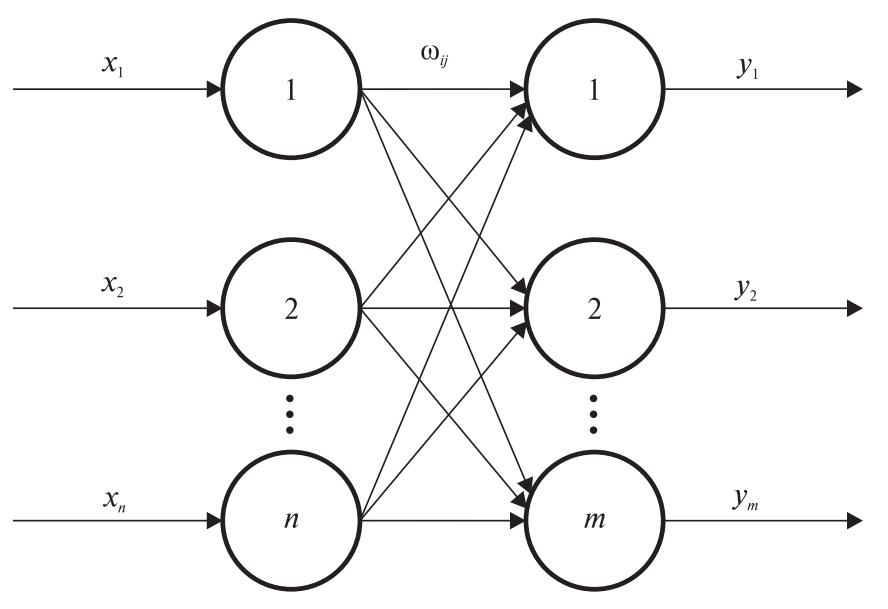
\includegraphics[width=0.4\linewidth]{figures/sd_ps/sd_ann/neural_network.png}}
	}

    \scnrelfrom{разбиение}{\scnkeyword{Типология и.н.с. по признаку направленности связей\scnsupergroupsign}}
    \scnaddlevel{1}
        \scneqtoset{
        искусственная нейронная сеть с прямыми связями\\
        \scnaddlevel{1}
            \scnsubdividing{
                персептрон\\
                \scnaddlevel{1}
                    \scnsubdividing{
                        персептрон Розенблатта;
                        автоэнкодерная искусственная нейронная сеть
                    }
                \scnaddlevel{-1}
                ;машина опорных векторов
                ;искусственная нейронная сеть радиально-базисных функций
            }
        \scnaddlevel{-1}
        ;искусственная нейронная сеть с обратными связями\\
        \scnaddlevel{1}
            \scnsubdividing{
                нейронная сеть Хопфилда
                ;нейронная сеть Хэмминга
            }
        \scnaddlevel{-1}
        ;рекуррентная искусственная нейронная сеть\\
        \scnaddlevel{1}
            \scnsubdividing{
            искусственная нейронная сеть Джордана
            ;искусственная нейронная сеть Элмана
            ;мультирекуррентная нейронная сеть
            ;LSTM-элемент
            ;GRU-элемент
            }
        \scnaddlevel{-1}
        }
    \scnaddlevel{-1}

    \scnrelfrom{разбиение}{\scnkeyword{Типология и.н.с. по признаку полноты связей\scnsupergroupsign}}
    \scnaddlevel{1}
        \scneqtoset{
        полносвязная искусственная нейронная сеть\\
        ;слабосвязная искусственная нейронная сеть
        }
    \scnaddlevel{-1}

    \scnrelfrom{решаемые задачи}{задачи, которые могут быть решены с помощью и.н.с. с приемлемой точностью}{
    \scnaddlevel{1}
    \scneqtoset{
        задача классификации\\
        \scnaddlevel{1}
            \scnsubset{задача}
            \scnexplanation{Задача построения классификатора, т.е. отображения $\tilde c: X \rightarrow C$, где $ X \in \mathbb{R}^m$ --
            признаковое пространство п.в.а., $C = {C_1, C_2, ...C_k }$ -- конечное и обычно небольшое множество меток классов.}
        \scnaddlevel{-1}
        ;задача регрессии\\
        \scnaddlevel{1}
            \scnsubset{задача}
            \scnexplanation{Задача построения оценочной функции по примерам $(x_i, f(x_i))$, где $f(x)$ -- неизвестная функция}
            \scnexplanation{\textbf{\textit{оценочная функция}} -- отображение вида $\tilde{f}: X \rightarrow \mathbb{R}$, где $X \in \mathbb{R}^m$ -- признаковое пространство п.в.а.}
        \scnaddlevel{-1}
        ;задача кластеризация\\
        \scnaddlevel{1}
            \scnsubset{задача}
            \scnexplanation{Задача разбиения множества п.в.а. на группы (кластеры) по какой-либо метрике сходства.}
        \scnaddlevel{-1}
        ;задача понижения размерности\\
        \scnaddlevel{1}
            \scnsubset{задача}
            \scnidtf{задача уменьшения размерности признакового пространства}
        \scnaddlevel{-1}
        ;задача управления\\
        \scnaddlevel{1}
            \scnsubset{задача}
        \scnaddlevel{-1}
        ;задача фильтрации\\
        \scnaddlevel{1}
            \scnsubset{задача}
        \scnaddlevel{-1}
        ;задача детекции\\
        \scnaddlevel{1}
            \scnsubset{задача}
            \scnsubset{задача классификации}
            \scnsubset{задача регрессии}
        \scnaddlevel{-1}
        ;задача с ассоциативной памятью\\
        \scnaddlevel{1}
            \scnsubset{задача}
        \scnaddlevel{-1}
    }
    }

\scnheader{формальный нейрон}
    \scnidtf{искусственный нейрон}
    \scnidtf{нейрон}
    \scnidtf{ф.н.}
    \scnidtf{нейронный элемент}
    \scnidtf{множество нейронов искусственных нейронных сетей}
    \scnidtf{математическая модель реального биологического нейрона}
    \scnnote{Отдельный формальный нейрон является искусственной нейронной сети с одним нейроном в единственном слое.}
    \scnsubset{искусственная нейронная сеть}
    \scnexplanation{\textbf{\textit{формальный нейрон}} -- это основной элемент \textit{искусственной нейронной сети}, применяющий свою \textit{функцию активации} (\scncite{Golovko2017}) к сумме произведений входных сигналов на весовые коэффициенты:
        \begin{equation*}
            y = F\left(\sum_{i=1}^{n} w_ix_i - T\right) = F(WX - T)
        \end{equation*}
        где $X = (x_1,x_2,...,x_n)^{T}$ -- вектор входного сигнала; $W - (w_1,w_2,...,w_n)$ -- вектор весовых коэффициентов; \textit{T} -- пороговое значение;
        \textit{F} -- функция активации.
    }

    \scnrelfrom{изображение}{
        \scnfileimage{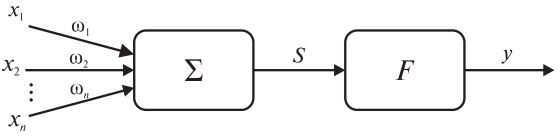
\includegraphics[width=0.4\linewidth]{figures/sd_ps/sd_ann/neuron.png}}
    }

    \scnnote{Формальные нейроны могут иметь полный набор связей с нейронами предшествующего слоя или неполный (разряженный)
        набор связей.}

    \scnsubdividing{
        полносвязный формальный нейрон\\
        \scnaddlevel{1}
            \scnidtf{нейрон, у которого есть полный набор связей с нейронами предшествующего слоя}
            \scnexplanation{отдельный обрабатывающий элемент и.н.с., выполняющий функциональное преобразование взвешенной суммы элементов вектора входных значений с помощью функции активации}
        \scnaddlevel{-1}
        ;сверточный формальный нейрон\\
        \scnaddlevel{1}
            \scnexplanation{Отдельный обрабатывающий элемент и.н.с., выполняющий функциональное преобразование результата
                операции свертки матрицы входных значений с помощью функции активации.}
            \scnnote{Сверточный формальный нейрон может быть представлен полносвязным формальным нейроном} 
            %\scnnote{Сверточный формальный нейрон с соответствующим ему ядром свертки может быть представлен нейроном с неполным набором связей.}
        \scnaddlevel{-1}
        ;рекуррентный формальный нейрон\\
        \scnaddlevel{1}
            \scnexplanation{Формальный нейрон, имеющий обратную связь с самим собой или с другими нейронами и.н.с.}
        \scnaddlevel{-1}
    }

\scnheader{формальный нейрон\scnrolesign}
    \scnidtf{формальный нейронный элемент\scnrolesign}
    \scnidtf{нейронный элемент\scnrolesign}
    \scnidtf{нейрон\scnrolesign}
    \scniselement{ролевое отношение}
    \scnrelfrom{первый домен}{искусственная нейронная сеть}
    \scnrelfrom{второй домен}{формальный нейрон}
    \scnrelfrom{область определения}{искусственная нейронная сеть}
    \scnexplanation{\textbf{\textit{формальный нейрон\scnrolesign}} -- ролевое отношение, связывающее искусственную нейронную сеть с ее нейроном.}

\scnheader{пороговый формальный нейрон\scnrolesign}
    \scnidtf{пороговый нейронный элемент\scnrolesign}
    \scnidtf{пороговый нейрон\scnrolesign}
    \scniselement{ролевое отношение}
    \scnrelfrom{первый домен}{искусственная нейронная сеть}
    \scnrelfrom{второй домен}{формальный нейрон}
    \scnrelfrom{область определения}{искусственная нейронная сеть}
    \scnexplanation{\textbf{\textit{пороговый формальный нейрон\scnrolesign}} -- ролевое отношение, связывающее искусственную нейронную сеть с таким ее нейроном,
            выходное значение которого всегда равно -1.
    }
    \scnexplanation{Весовой коэффициент синаптической связи, выходящей из такого нейрона, является порогом для нейрона, в который
        данная синаптическая связь входит.}

\scnheader{синаптическая связь}
    \scnidtf{синапс}
    \scnsubset{ориентированная пара}
    \scndefinition{\textbf{\textit{синаптическая связь}} -- ориентированная пара, первым компонентом которой является нейрон, из
        которого исходит сигнал, а вторым компонентом -- нейрон, который принимает этот сигнал.
    }

\scnheader{синаптическая связь\scnrolesign}
    \scnidtf{синапс\scnrolesign}
    \scniselement{ролевое отношение}
    \scnrelfrom{первый домен}{искусственная нейронная сеть}
    \scnrelfrom{второй домен}{синаптическая связь}
    \scnrelfrom{область определения}{\scnstartsetlocal\scnendstructlocal\\
        \scnreltoset{объединение}{искусственная нейронная сеть;синапс}
    }
    \scndefinition{\textbf{\textit{синаптическая связь\scnrolesign}} -- ролевое отношение, связывающее искусственную нейронную сеть с ее синапсом.
    }

\scnheader{параметр и.н.с.}
    \scnsubset{параметр}
    \scnsubdividing{
        настраиваемый параметр и.н.с.\\
        \scnaddlevel{1}
            \scnidtf{параметр и.н.с., значение которого изменяется в ходе обучения}
            \scnsubdividing{
                весовой коэффициент синаптической связи;
                пороговое значение;
                ядро свертки
                \scnaddlevel{1}
                    \scnidtf{квадратная матрица произвольного порядка, элементы которой изменяются в процессе
                        обучения и.н.с.}
                    \scnnote{если сверточный формальный нейрон представить в виде полносвязного формального нейрона, соответствующее ядро свертки преобразуется в вектор весовых коэффициентов}
                \scnaddlevel{-1}
            }
        \scnaddlevel{-1}\\
        ;архитектурный параметр и.н.с.\\
        \scnaddlevel{1}
            \scnnote{Параметр и.н.с., определяющий ее архитектуру.}
            \scnsubdividing{количество слоев;количество нейронов; количество синапсов}
        \scnaddlevel{-1}
    }

\scnheader{весовой коэффициент синаптической связи}
    \scnidtf{вес синапса}
    \scnidtf{сила синаптической связи}
    \scnsubset{настраиваемый параметр}
    \scnexplanation{\textbf{\textit{весовой коэффициент синаптической связи}} -- это числовой коэффициент, который ставится в соответствие каждому
        синапсу нейронной сети и изменяется в процессе обучения.
    }
    \scnnote{Если сила синаптической связи отрицательна, то она называется \textit{тормозящей}. В противном случае она
        является \textit{усиливающей}.
    }

\scnheader{входное значение формального нейрона*}
    \scnidtf{входное значение нейрона*}
    \scnidtf{входное значение*}
    \scniselement{неролевое отношение}
    \scniselement{бинарное отношение}
    \scnrelfrom{первый домен}{формальный нейрон}
    \scnrelfrom{второй домен}{число}
    \scnrelfrom{область определения}{\scnstartsetlocal\scnendstructlocal\\
        \scnreltoset{объединение}{формальный нейрон;число}
    }
    \scnexplanation{\textbf{\textit{входное значение формального нейрона*}} -- неролевое отношение, связывающее нейрон входного слоя со
        значением признака п.в.а., который подается на вход нейронной сети.
    }
    \scntext{теоретическая неточность}{Использование множества как формы представления входных данных является серьезным допущением, так как на практике
        входные данные структурированы более сложно -- в многомерные массивы. Самым близким теоретическим аналогом
        здесь выступает тензор. К сожалению, описание теории нейронных сетей с помощью тензорного исчисления в литературе
        как таковое отсутствует, но активно используется на практике: например, во многих разрабатываемых нейросетевых фреймворках.
        Формализация нейронных сетей с помощью тензоров видится авторам наиболее вероятным направлением работы в
        ближайших изданиях \textit{стандарта OSTIS}.
    }

\scnheader{паттерн входной активности и.н.с.}
	\scnidtf{п.в.а.}
    \scniselement{мультимножество}
    \scniselement{кортеж}
    \scnexplanation{\textbf{\textit{паттерн входной активности и.н.с.}} -- ориентированное мультимножество численных значений
        признаков некоторого объекта, которые могут выступать в качестве входных значений нейронов.
    }
	\scnnote{В текущей версии \textit{Стандарта OSTIS} предполагается, что п.в.а. содержит только предобработанные данные,
        то есть данные приведенные к численному виду и, возможно, преобразованные с помощью известных статистических
        методов (например, нормирования).
    }

\scnheader{признак}
    \scnidtf{feature}
    \scnidtf{множество признаков}
    \scnsubset{ролевое отношение}
    \scnexplanation{\textbf{\textit{признак}} -- множество ролевых отношений, каждое из которых связывает некоторый п.в.а. с численным значением, которое характеризует данный п.в.а. с какой-либо стороны.
    }

\scnheader{функция активации*}
    \scnidtf{функция активации нейрона*}
    \scniselement{неролевое отношение}
    \scniselement{бинарное отношение}
    \scnexplanation{\textbf{\textit{функция активации*}} -- неролевое отношение, связывающее формальный нейрон с функцией, результат
        применения которой к \textbf{\textit{взвешенной сумме нейрона}} определяет его \textbf{\textit{выходное значение}}.
    }
    \scnrelfrom{область определения}{\scnstartsetlocal\scnendstructlocal\\
        \scnreltoset{объединение}{формальный нейрон;функция}
    }
    \scnrelfrom{первый домен}{формальный нейрон}
    \scnrelfrom{второй домен}{функция}
    \scnaddlevel{1}
    \scnsubdividing{
        линейная функция\\
        \scnaddlevel{1}
            \scntext{формула}{
                \begin{equation*}
                    y = kS
                \end{equation*}
                где \textit{k} -- коэффициент наклона прямой, \textit{S} -- в.с.
            }
        \scnaddlevel{-1}
        ;пороговая функция\\
        \scnaddlevel{1}
            \scntext{формула}{
                \begin{equation*}
                    y = sign(S) =
                    \begin{cases}
                        1, S > 0,\\
                        0, S \leq 0
                    \end{cases}
                \end{equation*}
            }
        \scnaddlevel{-1}
        ;сигмоидная функция\\
        \scnaddlevel{1}
            \scntext{формула}{
                \begin{equation*}
                    y = \frac{1}{1+e^{-cS}}
                \end{equation*}
                где \textit{с} > 0 -- коэффициент, характеризующий ширину сигмоидной функции по оси абсцисс, \textit{S} -- в.с.
            }
        \scnaddlevel{-1}
        ;функция гиперболического тангенса\\
        \scnaddlevel{1}
            \scntext{формула}{
                \begin{equation*}
                    y = \frac{e^{cS}-e^{-cS}}{e^{cs}+e^{-cS}}
                \end{equation*}
                где \textit{с} > 0 -- коэффициент, характеризующий ширину сигмоидной функции по оси абсцисс, \textit{S} -- в.с.
            }
        \scnaddlevel{-1}
        ;функция softmax\\
        \scnaddlevel{1}
            \scntext{формула}{
                \begin{equation*}
                    y_j = softmax(S_j) = \frac{e^{S_j}}{\sum_{j} e^{S_j}}
                \end{equation*}
                где $S_j$ -- в.с. \textit{j}-го выходного нейрона
            }
        \scnaddlevel{-1}
        ;функция ReLU\\
        \scnaddlevel{1}
            \scntext{формула}{
                \begin{equation*}
                    y = F(S) =
                    \begin{cases}
                        S, S > 0,\\
                        kS, S \leq 0
                    \end{cases}
                \end{equation*}
                где \textit{k} = 0 или принимает небольшое значение, например, 0.01 или 0.001.
            }
        \scnaddlevel{-1}
    }
    \scnaddlevel{-1}

\scnheader{взвешенная сумма*}
    \scnidtf{взвешенная сумма входных значений*}
    \scnidtf{в.с.}
    \scniselement{неролевое отношение}
    \scniselement{бинарное отношение}
    \scnexplanation{\textbf{\textit{взвешенная сумма*}} -- неролевое отношение, связывающее формальный нейрон с числом, являющимся суммой
        произведений входных сигналов на весовые коэффициенты входящих в нейрон синаптических связей.
    }
    \scnrelfrom{область определения}{\scnstartsetlocal\scnendstructlocal\\
        \scnreltoset{объединение}{формальный нейрон;число}
    }
    \scnrelfrom{первый домен}{формальный нейрон}
    \scnrelfrom{второй домен}{число}
    \scnrelfrom{формула}{
        \begin{equation*}
            S = \sum_{i=1}^{n} w_ix_i - T
        \end{equation*}
        где \textit{n} -- размерность вектора входных значений, $w_i$ -- \textit{i}-тый элемент вектора весовых
        коэффициентов, $x_i$ -- \textit{i}-тый элемент вектора входных значений, \textit{T} -- пороговое значение.
    }

\scnheader{выходное значение формального нейрона*}
    \scnidtf{выходное значение нейрона*}
    \scnidtf{выходное значение*}
    \scniselement{неролевое отношение}
    \scniselement{бинарное отношение}
    \scnrelfrom{первый домен}{формальный нейрон}
    \scnrelfrom{второй домен}{число}
    \scnrelfrom{область определения}{\scnstartsetlocal\scnendstructlocal\\
        \scnreltoset{объединение}{формальный нейрон;число}
    }
    \scnexplanation{\textbf{\textit{входное значение*}} -- неролевое отношение, связывающее нейрон с числом, являющимся результатом применения
        функции активации нейрона к его взвешенной сумме.
    }
    \scnnote{Выходное значение нейрона является одним из входных сигналов для всех нейронов, в которые ведут выходящие из данного нейрона синапсы.
    }

\scnheader{слой и.н.с.}
    \scnidtf{слой}
    \scnidtf{слой искусственной нейронной сети}
    \scnidtf{множество слоев искусственных нейронных сетей}
    \scnnote{отдельный слой является искусственной нейронной сетью с одним слоем}
    \scnsubset{искусственная нейронная сеть}
    \scnexplanation{\textbf{\textit{слой и.н.с}}  -- это множество нейронных элементов, на которые в каждый такт времени
        параллельно поступает информация от других нейронных элементов сети (\scncite{Golovko2017})
    }
    \scnexplanation{\textbf{\textit{слой и.н.с.}} -- это множество формальных нейронов, осуществляющих параллельную независимую обработку
        вектора или матрицы входных значений
    }
    \scnnote{функция активации слоя является функцией активации всех формальных нейронов этого слоя}
    \scnnote{конфигурация слоя задается типом, количеством формальных нейронов, функцией активации}
    \scnnote{описание последовательности слоев и.н.с. с конфигурацией каждого слоя задает архитектуру и.н.с.}

    \scnsubdividing{
        полносвязный слой и.н.с.\\
        \scnaddlevel{1}
            \scnidtf{слой, в котором каждый нейрон имеет связь с каждым нейроном предшествующего слоя}
            \scnidtf{слой, в котором каждый нейрон является полносвязным}
        \scnaddlevel{-1}
        ;сверточный слой и.н.с.\\
        \scnaddlevel{1}
            \scnidtf{слой, в котором каждый нейрон является сверточным}
        \scnaddlevel{-1}
        ;слой и.н.с. нелинейного преобразования\\
        \scnaddlevel{1}
            \scnidtf{слой, осуществляющий нелинейное преобразование входных данных}
            \scnexplanation{Как правило, выделяются в отдельные слои только в программных реализациях. Фактически
                рассматриваются как финальный этап расчета выходной активности любого нейрона -- применение функции
                активации.}
            \scnnote{не изменяет размерность входных данных}
        \scnaddlevel{-1}
        ;dropout слой и.н.с.\\
        \scnaddlevel{1}
            \scnidtf{слой, реализующий технику регуляризации dropout}
            \scnnote{Данный тип слоя функционирует только во время обучения и.н.с.}
            \scnexplanation{Поскольку полносвязные слои имеют большое количество настраиваемых параметров, они
                подвержены эффекту переобучения. Один из способов устранить такой негативный эффект -- выполнить
                частичный отсев результатов на выходе полносвязного слоя. На этапе обучения техника dropout позволяет
                отбросить выходную активность некоторых нейронов с определенной, заданной вероятностью. Выходная
                активность ``отброшенных'' нейронов полагается равной нулю.}
        \scnaddlevel{-1}
        ;pooling слой и.н.с.\\
        \scnaddlevel{1}
            \scnidtf{подвыборочный слой}
            \scnidtf{объединяющий слой}
            \scnidtf{слой, осуществляющий уменьшение размерности входных данных}
        \scnaddlevel{-1}
        ;слой и.н.с. батч-нормализации\\
    }

\scnheader{распределяющий слой*}
    \scnidtf{входной слой*}
    \scniselement{неролевое отношение}
    \scniselement{бинарное отношение}
    \scndefinition{\textbf{\textit{распределяющий слой*}} -- неролевое отношение, связывающее искусственную нейронную сеть с ее слоем,
        нейроны которого принимают входные значения всей нейронной сети.
    }
    \scnrelfrom{область определения}{искусственная нейронная сеть}
    \scnrelfrom{первый домен}{искусственная нейронная сеть}
    \scnrelfrom{второй домен}{слой и.н.с.}

\scnheader{обрабатывающий слой*}
    \scniselement{неролевое отношение}
    \scniselement{бинарное отношение}
    \scndefinition{\textbf{\textit{обрабатывающий слой*}} -- неролевое отношение, связывающее искусственную нейронную сеть с ее слоем,
        нейроны которого принимают на вход выходные значения нейронов предыдущего слоя.
    }
    \scnrelfrom{область определения}{искусственная нейронная сеть}
    \scnrelfrom{первый домен}{искусственная нейронная сеть}
    \scnrelfrom{второй домен}{слой и.н.с}

\scnheader{выходной слой*}
    \scniselement{неролевое отношение}
    \scniselement{бинарное отношение}
    \scnexplanation{\textbf{\textit{выходной слой*}} -- неролевое отношение, связывающее искусственную нейронную сеть с ее слоем,
        выходные значения нейронов которого являются выходными значениями всей нейронной сети.
    }
    \scnrelfrom{область определения}{искусственная нейронная сеть}
    \scnrelfrom{первый домен}{искусственная нейронная сеть}
    \scnrelfrom{второй домен}{слой и.н.с}

\bigskip
\scnendstruct \scnendsegmentcomment{Предметная область и онтология искусственных нейронных сетей}

\scnsegmentheader{Предметная область и онтология действий по обработке искусственной нейронной сети}
\scnstartsubstruct

\newpage
\scnheader{Предметная область действий по обработке искусственных нейронных сетей}
    \scnidtf{Предметная область действий по обработке и.н.с.}
    \scniselement{предметная область}
    \scnsdmainclass{действие по обработке искусственных нейронных сетей}
    \scnsdclass{
        действие по обработке искусственных нейронных сетей;
        действие конфигурации весовых коэффициентов и.н.с.;
        действие конфигурации и.н.с.;
        действие интерпретации и.н.с.;
        метод обучения и.н.с.;
        метод обучения с учителем;
        метод обратного распространения ошибки;
        метод обучения без учителя;
        метод оптимизации;
        функция потерь;
        параметр обучения;
        скорость обучения;
        моментный параметр;
        параметр регуляризации;
        размер группы обучения;
        количество эпох обучения;
        выборка
    }
    \scnsdrelation{
        обучающая выборка\scnrolesign;
        тестовая выборка\scnrolesign;
        валидационная выборка\scnrolesign;
        метод обучения\scnrolesign;
        метод оптимизации\scnrolesign;
        функция потерь\scnrolesign
    }

\scnheader{действие по обработке искусственной нейронной сети}
    \scnidtf{действие по обработке и.н.с.}
    \scnidtf{действие с искусственной нейронной сетью}
    \scnsubset{действие}
    \scnexplanation{В зависимости от того, является ли искусственная нейронная сеть знаком внешней по отношению к памяти системы сущности,
        элементы множества действие по обработке и.н.с. являются либо элементами множества \textbf{\textit{действие, выполняемое кибернетической
        системой в своей внешней среде}}, либо элементом множества \textbf{\textit{действие, выполняемое кибернетической системой
        в собственной памяти.
    }}.
    }
    \scnsubdividing{
        действие конфигурации и.н.с.\\
        \scnaddlevel{1}
        \scnsubdividing{
            действие создания и.н.с.
            ;действие редактирования и.н.с.
            ;действие удаления и.н.с.
            ;действие конфигурации слоя и.н.с.\\
            \scnaddlevel{1}
                \scnsubdividing{
                    действие добавления слоя в и.н.с.
                    ;действие редактирования слоя и.н.с.
                    ;действие удаления слоя и.н.с.
                    ;действие установки функции активации нейронов слоя и.н.с.
                    ;действие конфигурации нейрона в слое и.н.с\\
                    \scnaddlevel{1}
                        \scnsubdividing{
                            действие добавления нейрона в слой и.н.с.
                            ;действие редактирования нейрона в слое и.н.с.
                            ;действие удаления нейрона из слоя и.н.с.
                            ;действие установки функции активации нейрона в слое и.н.с.
                        }
                    \scnaddlevel{-1}
                }
            \scnaddlevel{-1}
        }
        \scnaddlevel{-1}
        ;действие конфигурации весовых коэффициентов и.н.с.\\
        \scnaddlevel{1}
            \scnsuperset{действие обучения и.н.с.}
            \scnsuperset{действие начальной инициализации весов и.н.с.}
            \scnaddlevel{1}
                \scnsuperset{действие начальной инициализации весов нейронов слоя и.н.с.}
                \scnaddlevel{1}
                    \scnsuperset{действие начальной инициализации весов нейрона и.н.с.}
                \scnaddlevel{-1}
            \scnaddlevel{-1}
        \scnaddlevel{-1}
        ;действие интерпретации и.н.с.
    }
    \scnnote{Действия по обработке и.н.с осуществляет соответствующий коллектив агентов.}
    \scnexplanation{Так как в результате действий по обработке и.н.с объект этих действий, конкретная и.н.с, может существенно меняться
        (меняется конфигурация сети, ее весовые коэффициенты), то и.н.с представляется в базе знаний как темпоральное объединение
        всех ее версий. Каждая версия является и.н.с. и темпоральной сущностью. На множестве этих темпоральных сущностей задается
        темпоральная последовательность с указанием первой и последней версии. Для каждой версии описываются специфичные знания.
        Общие для всех версий знания описываются для и.н.с, являющейся темпоральным объединением всех версий.
    }
    \scnaddlevel{1}
        \scnrelfrom{пример}{
            \scnfilescg{figures/sd_ps/sd_ann/temporal_neural_network_scg.png}
        }
    \scnaddlevel{-1}

\scnheader{действие обучения и.н.с.}
    \scnidtf{действие обучения искусственной нейронной сети}
    \scnsubset{действие конфигурации весовых коэффициентов и.н.с.}
    \scndefinition{\textbf{\textit{действие обучения и.н.с.}} -- действие, в ходе которого реализуется определенный метод обучения
        и.н.с. с заданными параметрами обучения и.н.с, методом оптимизации и функцией потерь.
    }
    \scnrelfromset{известные проблемы}{
        \scnfileitem{Переобучение -- проблема, возникающая при обучении и.н.с., заключающаяся в том,
        что сеть хорошо адаптируется к п.в.а. из обучающей выборки, при этом теряя способность к обобщению.
        Переобучение возникает из-за применения неоправданно сложной модели при обучении и.н.с. Это происходит,
        когда количество настраиваемых параметров и.н.с. намного больше размера обучающей выборки. Возможные
        варианты решения проблемы заключаются в упрощении модели, увеличении выборки, использовании регуляризации
        (параметр регуляризации, техника dropout и т.д.).\\
        Обнаружение переобученности сложнее, чем недообученности. Как правило, для этого применяется
        кросс-валидация на валидационной выборке, позволяющая оценить момент завершения процесса обучения.
        Идеальным вариантом является достижение баланса между переобученностью и недообученностью.
        };
        \scnfileitem{Недообучение -- проблема, возникающая при обучении и.н.с., заключающаяся в том,
        что сеть дает одинаково плохие результаты на обучающей и контрольной выборках.
        Чаще всего такого рода проблема возникает при недостаточном времени, затраченном на обучение модели.
        Однако это может быть вызвано и слишком простой архитектурой модели либо малым размером обучающей
        выборки. Соответственно решение, которое может быть принято ML-инженером, заключается в устранении
        этих недостатков: увеличение времени обучения, использование модели с большим числом настраиваемых
        параметров, увеличение размера обучающей выборки, а также уменьшение регуляризации и более тщательный
        отбор признаков для обучающих примеров.
        }
    }
    \scnrelfrom{описание примера}{
        \scnfilescg{figures/sd_ps/sd_ann/ann_trainning_scg.png}
    }

\scnheader{выборка}
    \scnsubset{множество}
	\scnexplanation{\textbf{\textit{выборка}} -- множество п.в.а., используемых в процессе обучения, тестирования
        и архитектурной настройки и.н.с.
    }

\scnheader{обучающая выборка\scnrolesign}
    \scnidtf{training set\scnrolesign}
    \scniselement{ролевое отношение}
    \scnrelfrom{первый домен}{действие обучения и.н.с.}
    \scnrelfrom{второй домен}{выборка}
    \scnrelfrom{область определения}{\scnstartsetlocal\scnendstructlocal\\
        \scnreltoset{объединение}{действие обучения и.н.с.;выборка}
    }
    \scnexplanation{\textbf{\textit{обучающая выборка\scnrolesign}} -- ролевое отношение, связывающее действие обучения и.н.с. с выборкой,
        используемой для изменения настраиваемых параметров и.н.с. в процессе ее обучения.
    }

\scnheader{тестовая выборка\scnrolesign}
    \scnidtf{test set\scnrolesign}
    \scniselement{ролевое отношение}
    \scnrelfrom{первый домен}{действие обучения и.н.с.}
    \scnrelfrom{второй домен}{выборка}
    \scnrelfrom{область определения}{\scnstartsetlocal\scnendstructlocal\\
        \scnreltoset{объединение}{действие обучения и.н.с.;выборка}
    }
    \scnexplanation{\textbf{\textit{тестовая выборка\scnrolesign}} -- ролевое отношение, связывающее действие обучения и.н.с. с выборкой,
        используемой для проверки обобщающей способности обученной и.н.с.
    }
    \scnnote{Элементы контрольной выборки не используются в процессе обучения.}
\right) 
\scnheader{валидационная выборка\scnrolesign}
    \scniselement{ролевое отношение}
    \scnrelfrom{первый домен}{действие обучения и.н.с.}
    \scnrelfrom{второй домен}{выборка}
    \scnrelfrom{область определения}{\scnstartsetlocal\scnendstructlocal\\
        \scnreltoset{объединение}{действие обучения и.н.с.;выборка}
    }
    \scnexplanation{\textbf{\textit{валидационная выборка\scnrolesign}} -- ролевое отношение, связывающее действие обучения и.н.с. с выборкой,
        используемой для определения (настройки) архитектурных параметров и.н.с. и параметров обучения.
    }
    \scnnote{Элементы валидационной выборки не используются в процессе обучения (не входят в обучающую выборку).}


\scnheader{метод обучения и.н.с.}
    \scnsubset{метод}
	\scnexplanation{\textbf{\textit{метод обучения и.н.с.}} -- метод итеративного поиска оптимальных значений настраиваемых параметров и.н.с.,
        минимизирующих некоторую заданную функцию потерь.
    }
	\scnnote{Стоит отметить, что хотя целью применения метода обучения является минимизация функции потерь, ``полезность''
        полученной после обучения модели можно оценить только по достигнутому уровню ее обобщающей способности.
    }
	\scnsuperset{метод обучения с учителем}
	\scnaddlevel{1}
		\scnexplanation{
            \textbf{\textit{метод обучения с учителем}} -- метод обучения с использованием заданных целевых переменных.
        }
		\scnsuperset{метод обратного распространения ошибки}
		\scnaddlevel{1}
			\scnidtf{м.о.р.о.}
			\scntext{алгоритм}{\\
				\begin{minipage}{\linewidth}
					\vspace{-\baselineskip}
					\begin{algorithm}[H]
						\KwData{$X$ -- данные, $Et$ -- желаемый отклик (метки), $E_m$ -- желаемая ошибка (в соответствии с выбранной функцией потерь)}
						\KwResult{обученная нейронная сеть \textit{Net}}
						инициализация весов \textit{W} и порогов \textit{T};\\
						\Repeat{$E<E_m$}{
							\ForEach{$x \in X$ \And $e \in Et$}{
								фаза прямого распространения сигнала: вычисляются активации для всех слоев и.н.с.;\\
								фаза обратного распространения ошибки: вычисляются ошибки для последнего слоя и всех предшествующих слоев;\\
								изменение настраиваемых параметров и.н.с. в соответствии с вычисленными ошибками;\\
							}
							вычисление общей ошибки E на данной эпохе;
						}
					\end{algorithm}
				\end{minipage}
            }
			\scnnote{м.о.р.о. использует заданный метод оптимизации и заданную функцию потерь для реализации фазы
                обратного распространения ошибки и изменения настраиваемых параметров и.н.с. Одним из самых распространенных
                методов оптимизации является метод стохастического градиентного спуска. Приведенный м.о.р.о. используется
                для реализации последовательного варианта обучения.
            }
			\scnnote{Следует также отметить, что несмотря на то, что метод отнесен к методам обучения с учителем, в случае
                использования м.о.р.о. для обучения автокодировщиков в классических публикациях он рассматривается как
                метод обучения без учителя, поскольку в данном случае размеченные данные отсутствуют.
            }
		\scnaddlevel{-1}
	\scnaddlevel{-1}
	\scnsuperset{метод обучения без учителя}
	\scnaddlevel{1}
		\scnexplanation{\textbf{\textit{метод обучения без учителя}} -- метод обучения без использования заданных целевых переменных
            (в режиме самоорганизации)
        }
		\scnexplanation{В ходе выполнения алгоритма метода обучения без учителя выявляются полезные структурные свойства
            набора. Неформально его понимают как метод для извлечения информации из распределения, выборка для которого
            не была вручную аннотирована человеком (\scncite{Goodfellow2017}).
        }
	\scnaddlevel{-1}

\scnheader{метод обучения\scnrolesign}
    \scniselement{ролевое отношение}
    \scnrelfrom{первый домен}{действие обучения и.н.с.}
    \scnrelfrom{второй домен}{метод обучения и.н.с.}
    \scnrelfrom{область определения}{\scnstartsetlocal\scnendstructlocal\\
        \scnreltoset{объединение}{действие обучения и.н.с.;метод обучения и.н.с.}
    }
    \scnexplanation{\textbf{\textit{метод обучения\scnrolesign}} -- ролевое отношение, связывающее действие обучения и.н.с. с методом обучения,
        использующимся для обучения и.н.с. в рамках этого действия.
    }

\newpage
\scnheader{метод оптимизации}
    \scnsubset{метод}
	\scndefinition{\textbf{\textit{метод оптимизации}} -- метод для минимизации целевой функции потерь при обучении и.н.с.}
	\scnrelfromlist{включение}{
		SGD\\
		\scnaddlevel{1}
			\scnidtf{стохастический градиентный спуск}
			\scnidtf{с.г.с.}
			\scnidtf{stochastic gradient descent}
			\scnnote{В методе стохастического градиентного спуска корректировка настраиваемых параметров и.н.с. выполняется в направлении максимального уменьшения функции стоимости, т.е. в направлении, противоположном вектору градиента функции потерь (\scncite{Haykin2006})}
		\scnaddlevel{-1}
		;Nesterov method\\
		\scnaddlevel{1}
			\scnidtf{метод Нестерова}
			\scnnote{Обучение методом с.г.с. иногда происходит очень медленно. Импульсный метод позволяет ускорить обучение, особенно в условиях высокой кривизны, небольших, но устойчивых градиентов или зашумленных градиентов. В импульсном методе вычисляется экспоненциально затухающее скользящее среднее прошлых градиентов и продолжается движение в этом направлении. Метод Нестерова является вариантом импульсного алгоритма, в котором градиент вычисляется после применения текущей скорости (\scncite{Goodfellow2017})}
		\scnaddlevel{-1}
		;AdaGrad\\
		\scnaddlevel{1}
			\scnidtf{adaptive gradient}
			\scnnote{Данный метод по отдельности адаптирует скорости обучения всех настраиваемых параметров и.н.с., умножая их на коэффициент, обратно пропорциональный квадратному корню из суммы всех прошлых значений квадрата градиента (\scncite{Duchi2011})}
		\scnaddlevel{-1}
		;RMSProp\\
		\scnaddlevel{1}
			\scnidtf{root mean square propagation}
			\scnnote{Данный метод является модификацией AdaGrad, которая позволяет улучшить его поведение в невыпуклом случае путем изменения способа агрегирования градиента на экспоненциально взвешенное скользящее среднее. Использование экспоненциально взвешенного скользящего среднего гарантирует повышение скорости сходимости после обнаружения выпуклой впадины, как если бы внутри этой впадины алгоритм AdaGrad был инициализирован заново (\scncite{Goodfellow2017})}
		\scnaddlevel{-1}	
		;Adam\\
		\scnaddlevel{1}
			\scnidtf{adaptive moments}
			\scnnote{Данный метод можно рассматривать как комбинацию RMSProp и AdaGrad (\scncite{Kingma2014}). Помимо усредненного первого момента, данный метод использует усредненное значение вторых моментов градиентов}
		\scnaddlevel{-1}
	}
	\scnnote{Успешность применения методов оптимизации зависит главным образом от знакомства пользователя с соответствующим
        алгоритмом (\scncite{Goodfellow2017}).
    }

\scnheader{метод оптимизации\scnrolesign}
    \scniselement{ролевое отношение}
    \scnrelfrom{первый домен}{метод обучения и.н.с.}
    \scnrelfrom{второй домен}{метод оптимизации}
    \scnrelfrom{область определения}{\scnstartsetlocal\scnendstructlocal\\
        \scnreltoset{объединение}{метод обучения и.н.с.;метод оптимизации}
    }
    \scnexplanation{\textbf{\textit{метод оптимизации\scnrolesign}} -- ролевое отношение, связывающее метод обучения и.н.с. с методом оптимизации,
        использующимся для обучения и.н.с. с помощью данного метода.
    }

\scnheader{функция потерь}
    \scnsubset{функция}
	\scnexplanation{\textbf{\textit{функция потерь}} -- функция, используемая для вычисления ошибки, рассчитываемой как разница между фактическим
        эталонным значением и прогнозируемым значением, получаемым и.н.с.
    }
    \scnrelfromlist{включение}{
		MSE\\
		\scnaddlevel{1}
			\scnidtf{mean square error}
			\scnidtf{средняя квадратичная ошибка}
			\scntext{формула}{
				\begin{equation*}
					MSE = \frac{1}{L} \sum_{l=1}^L \sum_{i=1}^m (y_i^l - e_i^l)^2
				\end{equation*}
				где $y_i^l$ -- прогноз модели, $e_i^l$ -- ожидаемый (эталонный) результат, \textit{m} -- размерность выходного вектора, \textit{L} -- объем обучающей выборки.
			}
		\scnaddlevel{-1}
		;BCE\\
		\scnaddlevel{1}
			\scnidtf{binary cross entropy}
			\scnidtf{бинарная кросс-энтропия}
			\scntext{формула}{
				\begin{equation*}
					BCE = - \sum_{l=1}^L (e^l \log(y^l) + (1 - e^l)\log(1 - y^l))
				\end{equation*}
				где $y^l$ -- прогноз модели, $e^l$ -- ожидаемый (эталонный) результат: \textit{0} или \textit{1}, \textit{L} -- объем обучающей выборки.
			}
			\scnnote{для бинарной кросс-энтропии в выходном слое и.н.с. будет находиться один нейрон}
		\scnaddlevel{-1}
		;MCE\\
		\scnaddlevel{1}
			\scnidtf{multi-class cross entropy}
			\scnidtf{мультиклассовая кросс-энтропия}
			\scntext{формула}{
				\begin{equation*}
					MCE = - \sum_{l=1}^L \sum_{i=1}^m e_{i}^l \log(y_{i}^l)
				\end{equation*}
				где $y_{i}^l$ -- прогноз модели, $e_i^l$ -- ожидаемый (эталонный результат), \textit{m} -- размерность выходного вектора
			}
			\scnnote{для мультиклассовой кросс-энтропии количество нейронов в выходном слое и.н.с. совпадает с количеством классов}
		\scnaddlevel{-1}
	}
	\scnnote{Для решения задачи классификации рекомендуется использовать бинарную или мультиклассовую кросс-энтропийную функцию потерь,
        для решения задачи регрессии рекомендуется использовать среднюю квадратичную ошибку.
    }

\scnheader{функция потерь\scnrolesign}
    \scniselement{ролевое отношение}
    \scnrelfrom{первый домен}{метод обучения и.н.с.}
    \scnrelfrom{второй домен}{функция потерь}
    \scnrelfrom{область определения}{\scnstartsetlocal\scnendstructlocal\\
        \scnreltoset{объединение}{метод обучения и.н.с.;функция потерь}
    }
    \scnexplanation{\textbf{\textit{функция потерь\scnrolesign}} -- ролевое отношение, связывающее метод обучения и.н.с. с функцией потерь,
        использующимся для обучения и.н.с. с помощью данного метода.
    }

\scnheader{параметр обучения}
   \scnidtf{группа наиболее общих параметров метода обучения и.н.с.}
   \scnrelfromset{состав группы параметров обучения}{
       скорость обучения\\
          \scnaddlevel{1}
              \scnexplanation{\textbf{\textit{скорость обучения}} -- параметр, определяющий скорость изменения параметров и.н.с.
                в процессе обучения.
              }
          \scnaddlevel{-1}
       ;моментный параметр\\
          \scnaddlevel{1}
                \scnidtf{момент}
                \scnidtf{momentum}
                \scnexplanation{\textbf{\textit{моментный параметр}} -- параметр, используемый в процессе обучения для устранения
                    проблемы ``застревания'' алгоритма обучения в локальных минимумах минимизируемой функции потерь.
                }
                \scnexplanation{При обучении и.н.с. частой является ситуация остановки процесса в определенной точке локального
                    минимума без достижения желаемого уровня обобщающей способности и.н.с. Для устранения такого
                    нежелательного явления вводится дополнительный параметр (момент) позволяющий алгоритму обучения
                    ``перескочить'' через локальный минимум и продолжить процесс.
                }
         \scnaddlevel{-1}
       ;параметр регуляризации\\
         \scnaddlevel{1}
             \scnexplanation{\textbf{\textit{параметр регуляризации}} -- параметр, применяемый для контроля уровня переобучения и.н.с.
             }
             \scnexplanation{\textbf{\textit{регуляризация}} -- добавление дополнительных ограничений к правилам изменения настраиваемых
                параметров и.н.с. с целью предотвратить переобучение.
             }
         \scnaddlevel{-1}
       ;размер группы обучения\\
         \scnaddlevel{1}
             \scnexplanation{\textbf{\textit{размер группы обучения}} -- размер группы п.в.а., которая используется для изменения параметров
                и.н.с. на каждом элементарном шаге обучения.
             }
         \scnaddlevel{-1}
       ;количество эпох обучения\\
       \scnaddlevel{1}
       		\scnexplanation{\textbf{\textit{эпоха обучения}} -- одна итерация алгоритма обучения, в ходе которой все обучающие п.в.а.
                из обучающей выборки были однократно использованы.
            }
       \scnaddlevel{-1}
   }

\bigskip
\scnendstruct \scnendsegmentcomment{Предметная область и онтология действий по обработке искусственной нейронной сети}

\bigskip
\scnendstruct \scnendcurrentsectioncomment

\end{SCn}

\scchapter{Предметная область и онтология интерфейсов ostis-систем}
\label{sec:sd_interfaces}
\begin{SCn}
	
\scnsectionheader{\currentname}
	
\scnstartsubstruct

\scnrelfromlist{дочерний раздел}{Предметная область и онтологий интерфейсных действий пользователей ostis-систем;Предметная область и онтология естественных языков}

\scnheader{Предметная область интерфейсов ostis-систем}
\scniselement{предметная область}
\scnsdmainclasssingle{пользовательский интефейс}
\scnsdclass{командный пользовательский интерфейс;графический пользовательский интерфейс;WIMP-интерфейс;SILK-интерфейс;естественно-языковой интерфейс;речевой интерфейс;пользовательский интерфейс ostis-системы;компонент пользовательского интерфейса;атомарный компонент пользовательского интерфейса;неатомарный компонент пользовательского интерфейса;визуальная часть пользовательского интерфейса ostis-системы;компонент пользовательского интерфейса для представления;компонент вывода;компонент выполнения;параграф;декоративный компонент пользовательского интерфейса;контейнер;меню;строка меню;панель инструментов;панель вкладок;окно;модальное окно;немодальное окно;интерактивный компонент пользовательского интерфейса;флаговая кнопка;радиокнопка;переключатель;кнопка-счетчик;полоса прокрутки;кнопка}


\scnheader{пользовательский интерфейс}
\scnsuperset{командный пользовательский интерфейс}
\scnsuperset{графический пользовательский интерфейс}
\scnaddlevel{1}
\scnsuperset{WIMP-интерфейс}
\scnaddlevel{1}
\scnsuperset{пользовательский интерфейс ostis-системы}
\scnaddlevel{1}
\scnhaselement{Пользовательский интерфейс Метасистемы IMS.ostis}
\scnhaselement{Пользовательский интерфейс ИСС по геометрии}
\scnaddlevel{1}
\scnidtf{Пользовательский интерфейс интеллектуальной справочной системы по геометрии}
\scnaddlevel{-1}
\scnhaselement{Пользовательский интерфейс ИСС по дискретной математике}
\scnaddlevel{1}
\scnidtf{Пользовательский интерфейс интеллектуальной справочной системы по дискретной математике}
\scnaddlevel{-1}
\scnhaselement{Пользовательский интерфейс ИСС по географии}
\scnaddlevel{1}
\scnidtf{Пользовательский интерфейс интеллектуальной справочной системы по географии}
\scnaddlevel{-1}
\scnhaselement{Пользовательский интерфейс ИСС по искусственным нейронным сетям}
\scnaddlevel{1}
\scnidtf{Пользовательский интерфейс интеллектуальной справочной системы по искусственным нейронным сетям}
\scnaddlevel{-1}
\scnhaselement{Пользовательский интерфейс ИСС по лингвистике}
\scnaddlevel{1}
\scnidtf{Пользовательский интерфейс интеллектуальной справочной системы по лингвистике}
\scnaddlevel{-3}
\scnsuperset{SILK-интерфейс}
\scnaddlevel{1}
\scnidtf{(Speech – речь, Image – образ, Language – язык, Knowledge – знание)}
\scnsuperset{естественно-языковой интерфейс}
\scnaddlevel{1}
\scnsuperset{речевой интерфейс}
\scnaddlevel{-2}

\scnheader{пользовательский интерфейс}
\scnexplanation{\textit{пользовательский интерфейс} -- один из наиболее важных компонентов компьютерной системы. Представляет собой совокупность аппаратных и программных средств, обеспечивающих обмен информацией между пользователем и компьютерной системой.}

\scnheader{командный пользовательский интерфейс}
\scnexplanation{\textit{командный пользовательский интерфейс} -- пользовательский интерфейс, при котором обмен информацией между компьютерной системой и пользователем осуществляется путем написания текстовых инструкций или команд.}

\scnheader{графический пользовательский интерфейс}
\scnexplanation{\textit{графический пользовательский интерфейс} -- пользовательский интерфейс, при котором обмен информацией между компьютерной системой и пользователем осуществляется при помощи графических компонентов компьютерной системы.}

\scnheader{WIMP-интерфейс}
\scnexplanation{\textit{WIMP-интерфейс} -- пользовательский интерфейс, при котором обмен информацией между компьютерной системой и пользователем осуществляется в форме диалога при помощью окон, меню и других элементов управления.}

\scnheader{SILK-интерфейс}
\scnexplanation{\textit{SILK-интерфейс} -- пользовательский интерфейс, наиболее приближенный к естественной для человека форме общения. Компьютерная система находит для себя команды, анализируя человеческую речь и находя в ней ключевые фразы. Результат выполнения команд преобразуется в понятную человеку форму, например, в естественно-языковую форму или изображение.}

\scnheader{естественно-языковой интерфейс}
\scnexplanation{\textit{естественно-языковой интерфейс} -- SILK-интерфейс, обмен информацией между компьютерной системой и пользователем в котором происходит за счёт диалога. Диалог ведётся на одном из естественных языков.}

\scnheader{речевой интерфейс}
\scnexplanation{\textit{речевой интерфейс} -- SILK-интерфейс, обмен информацией в котором происходит за счёт диалога, в процессе которого компьютерная система и пользователь общаются с помощью речи. Данный вид интерфейса наиболее приближен к естественному общению между людьми.}

\scnheader{пользовательский интерфейс ostis-системы}
\scnsubset{ostis-система}
\scnexplanation{\textit{пользовательский интерфейс ostis-системы} представляет собой специализированную \textit{ostis-систему}, ориентированную на решение интерфейсных задач, и имеющую в своем составе базу знаний и решатель задач пользовательского интерфейса ostis-системы.\\
Для решения задачи построения пользовательского интерфейса в базе знаний \textit{пользовательского интерфейса ostis-системы} необходимо наличие sc-модели \textit{компонентов пользовательского интерфейса}, \textit{интерфейсных действий пользователей}, а также классификации \textit{пользовательских интерфейсов} вцелом. При проектировании интерфейса используется компонентный подход,который предполагает представление всего интерфейса приложения в виде отдельных специфицированных компонентов, которые могут разрабатываться и совершенствоваться независимо.}

\scnheader{компонент пользовательского интерфейса}
\scnexplanation{\textit{компонент пользовательского интерфейса} -- знак фрагмента базы знаний, имеющий определённую форму внешнего представления на экране.}
\scnsubdividing{атомарный компонент пользовательского интерфейса;неатомарный компонент пользовательского интерфейса}

\scnheader{атомарный компонент пользовательского интерфейса}
\scnexplanation{\textit{атомарный компонент пользовательского интерфейса} -- компонент пользовательского интерфейса, не содержащий в своём составе других компонентов пользовательского интерфейса.}

\scnheader{неатомарный компонент пользовательского интерфейса}
\scnexplanation{\textit{неатомарный компонент пользовательского интерфейса} -- компонент пользовательского интерфейса, состоящий из других компонентов пользовательского интерфейса.}

\scnheader{визуальная часть пользовательского интерфейса ostis-системы}
\scnsubset{неатомарный компонент пользовательского интерфейса}
\scnexplanation{\textit{визуальная часть пользовательского интерфейса ostis-системы} -- часть базы знаний пользовательского интерфейса ostis-системы, содержащая необходимые для отображения пользовательского интерфейса компоненты.}
	
\scnheader{компонент пользовательского интерфейса}
\scnidtf{user interface component}
\scnsuperset{компонент пользовательского интерфейса для отображения}
\scnaddlevel{1}
\scnidtf{presentation user interface component}
\scnaddlevel{-1}
\scnaddlevel{1}
	\scnsuperset{компонент вывода}
	\scnaddlevel{1}
	\scnidtf{output}
	\scnaddlevel{-1}
	\scnaddlevel{1}
		\scnsuperset{компонент вывода изображения}
		\scnaddlevel{1}
		\scnidtf{image-output}
		\scnaddlevel{-1}
		\scnsuperset{компонент вывода графической информации}
		\scnaddlevel{1}
		\scnidtf{graphical-output}
		\scnaddlevel{-1}
			\scnaddlevel{1}
			\scnsuperset{диаграмма}
			\scnaddlevel{1}
			\scnidtf{chart}
			\scnaddlevel{-1}
			\scnsuperset{карта}
			\scnaddlevel{1}
			\scnidtf{map}
			\scnaddlevel{-1}
			\scnsuperset{индикатор выполнения} 
			\scnaddlevel{1}
			\scnidtf{progress-bar}
			\scnaddlevel{-1}
			\scnaddlevel{-1}
		\scnsuperset{компонент вывода видео}
		\scnaddlevel{1}
		\scnidtf{video-output}
		\scnaddlevel{-1}
		\scnsuperset{компонент вывода звука}
		\scnaddlevel{1}
		\scnidtf{sound-output}
		\scnaddlevel{-1}
		\scnsuperset{компонент вывода текста}
		\scnaddlevel{1}
		\scnidtf{text-output}
		\scnaddlevel{-1}
			\scnaddlevel{1}
			\scnsuperset{заголовок}
			\scnaddlevel{1}
			\scnidtf{headline}
			\scnaddlevel{-1}
			\scnsuperset{параграф}
			\scnaddlevel{1}
			\scnidtf{paragraph}
			\scnaddlevel{-1}
			\scnsuperset{сообщение}
			\scnaddlevel{1}
			\scnidtf{message}
			\scnaddlevel{-1}
			\scnaddlevel{-2}
\scnsuperset{декоративный компонент пользовательского интерфейса}
\scnaddlevel{1}
\scnidtf{decorative user interface component}
\scnaddlevel{-1}
	\scnaddlevel{1}
	\scnsuperset{разделитель}
	\scnaddlevel{1}
	\scnidtf{separator}
	\scnaddlevel{-1}
	\scnsuperset{пустое пространство}
	\scnaddlevel{1}
	\scnidtf{blank-space}
	\scnaddlevel{-2}
\scnsuperset{контейнер}
	\scnaddlevel{1}
		\scnidtf{container}
		\scnsuperset{меню}
		\scnaddlevel{1}
		\scnidtf{menu}
		\scnaddlevel{-1}
		\scnsuperset{строка меню}
		\scnaddlevel{1}
		\scnidtf{menu-bar}
		\scnaddlevel{-1}
		\scnsuperset{панель инструментов}
		\scnaddlevel{1}
		\scnidtf{tool-bar}
		\scnaddlevel{-1}
		\scnsuperset{строка состояния}
		\scnaddlevel{1}
		\scnidtf{status-bar}
		\scnaddlevel{-1}
		\scnsuperset{таблично-строковый контейнер}
		\scnaddlevel{1}
		\scnidtf{table-row-container}
		\scnaddlevel{-1}
		\scnsuperset{списковый контейнер}
		\scnaddlevel{1}
		\scnidtf{list-container}
		\scnaddlevel{-1}
		\scnsuperset{таблично-клеточный контейнер}
		\scnaddlevel{1}
		\scnidtf{table-cell-container}
		\scnaddlevel{-1}
		\scnsuperset{древовидный контейнер}
		\scnaddlevel{1}
		\scnidtf{tree-container}
		\scnaddlevel{-1}
		\scnsuperset{панель вкладок}
		\scnaddlevel{1}
		\scnidtf{tab-pane}
		\scnaddlevel{-1}
		\scnsuperset{панель вращения}
		\scnaddlevel{1}
		\scnidtf{spin-pane}
		\scnaddlevel{-1}
		\scnsuperset{узловой контейнер}
		\scnaddlevel{1}
		\scnidtf{tree-node-container}
		\scnaddlevel{-1}
		\scnsuperset{панель прокрутки}
		\scnaddlevel{1}
		\scnidtf{scroll-pane}
		\scnaddlevel{-1}
		\scnsuperset{окно}
		\scnaddlevel{1}
		\scnidtf{window}
		\scnaddlevel{-1}
			\scnaddlevel{1}
			\scnsuperset{модальное окно}
			\scnaddlevel{1}
			\scnidtf{modal-window}
			\scnaddlevel{-1}
			\scnsuperset{немодальное окно}
			\scnaddlevel{1}
			\scnidtf{non-modal-window}
			\scnaddlevel{-4}		
\scnsuperset{интерактивный компонент пользовательского интерфейса}
\scnaddlevel{1}
\scnidtf{interactive user interface component}
\scnaddlevel{-1}
	\scnaddlevel{1}
	\scnsuperset{компонент ввода данных}
	\scnaddlevel{1}
	\scnidtf{data-input-component}
	\scnaddlevel{-1}
		\scnaddlevel{1}
		\scnsuperset{компонент ввода данных с прямой ответной реакцией}
		\scnaddlevel{1}
		\scnidtf{data-input-component-with-direct-feedback}
		\scnaddlevel{-1}
			\scnaddlevel{1}
			\scnsuperset{компонент ввода текста с прямой ответной реакцией}
			\scnaddlevel{1}
			\scnidtf{text-input-component-with-direct-feedback}
			\scnaddlevel{-1}
				\scnaddlevel{1}
				\scnsuperset{многострочное текстовое поле}
				\scnaddlevel{1}
				\scnidtf{multi-line-text-field}
				\scnaddlevel{-1}
				\scnsuperset{однострочное текстовое поле}
				\scnaddlevel{1}
				\scnidtf{single-line-text-field}
				\scnaddlevel{-1}
				\scnaddlevel{-1}
			\scnsuperset{ползунок}
			\scnaddlevel{1}
			\scnidtf{slider}
			\scnaddlevel{-1}
			\scnsuperset{область рисования}
			\scnaddlevel{1}
			\scnidtf{drawing-area}
			\scnaddlevel{-1}
			\scnsuperset{компонент выбора}
			\scnaddlevel{1}
			\scnidtf{selection-component}
			\scnaddlevel{-1}
				\scnaddlevel{1}
				\scnsuperset{компонент выбора нескольких значений}
				\scnaddlevel{1}
				\scnidtf{selection-component-multiple-values}
				\scnaddlevel{-1}
				\scnsuperset{компонент выбора одного значения}
				\scnaddlevel{1}
				\scnidtf{selection-component-single-values}
				\scnaddlevel{-1}
				\scnaddlevel{-1}
			\scnsuperset{компонент выбора данных}
			\scnaddlevel{1}
			\scnidtf{selectable-data-representation}
			\scnaddlevel{-1}	
				\scnaddlevel{1}
				\scnsuperset{флаговая кнопка}
				\scnaddlevel{1}
				\scnidtf{check-box}
				\scnaddlevel{-1}
				\scnsuperset{радиокнопка}
				\scnaddlevel{1}
				\scnidtf{radio-button}
				\scnaddlevel{-1}
				\scnsuperset{переключатель}
				\scnaddlevel{1}
				\scnidtf{toggle-button}
				\scnaddlevel{-1}
				\scnsuperset{выбираемый элемент}
				\scnidtf{selectable-item}
				\scnaddlevel{-2}
		\scnsuperset{компонент ввода данных без прямой ответной реакции}
		\scnaddlevel{1}
		\scnidtf{data-input-component-without-direct-feedback}
		\scnaddlevel{-1}
			\scnaddlevel{1}
			\scnsuperset{кнопка-счётчик}
			\scnaddlevel{1}
			\scnidtf{spin-button}
			\scnaddlevel{-1}
			\scnsuperset{компонент речевого ввода}
			\scnaddlevel{1}
			\scnidtf{speech-input}
			\scnaddlevel{-1}
			\scnsuperset{компонент ввода движений}
			\scnaddlevel{1}
			\scnidtf{motion-input}
			\scnaddlevel{-1}
			\scnaddlevel{-2}
	\scnsuperset{компонент для представления и взаимодействия с пользователем}
	\scnaddlevel{1}
	\scnidtf{presentation-manipulation-component}
	\scnaddlevel{-1}
		\scnaddlevel{1}
		\scnsuperset{активирующий компонент}
		\scnaddlevel{1}
		\scnidtf{activating-component}
		\scnaddlevel{-1}
		\scnsuperset{компонент непрерывной манипуляции}
		\scnaddlevel{1}
		\scnidtf{continuous-manipulation-component}
		\scnaddlevel{-1}
			\scnaddlevel{1}
			\scnsuperset{полоса прокрутки}
			\scnaddlevel{1}
			\scnidtf{scrollbar}
			\scnaddlevel{-1}
			\scnsuperset{компонент редактирования размера}
			\scnaddlevel{1}
			\scnidtf{resizer}
			\scnaddlevel{-1}
			\scnaddlevel{-2}
	\scnsuperset{компонент запроса действий}
	\scnaddlevel{1}
	\scnidtf{operation-trigger-component}
	\scnaddlevel{-1}
		\scnaddlevel{1}
		\scnsuperset{компонент выбора команд}
		\scnaddlevel{1}
		\scnidtf{command-selection-component}
		\scnaddlevel{-1}
			\scnaddlevel{1}
			\scnsuperset{кнопка}
			\scnaddlevel{1}
			\scnidtf{button}
			\scnaddlevel{-1}
			\scnsuperset{пункт меню}
			\scnaddlevel{1}
			\scnidtf{menu-item}
			\scnaddlevel{-1}
			\scnaddlevel{-1}
		\scnsuperset{компонент ввода команд}
		\scnaddlevel{1}
		\scnidtf{command-input-component}
		\scnaddlevel{-1}
		\scnaddlevel{-2}

\scnheader{компонент пользовательского интерфейса для представления}
\scnexplanation{\textit{компонент пользовательского интерфейса для представления} -- компонент пользовательского интерфейса, не подразумевающий взаимодействия с пользователем.}

\scnheader{компонент вывода}
\scnexplanation{\textit{компонент вывода} -- компонент пользовательского интерфейса, предназначенный для представления информации.}

\scnheader{индикатор выполнения}
\scnexplanation{\textit{индикатор выполнения} -- компонент пользовательского интерфейса, предназначенный для отображения процента выполнения какой-либо задачи.}

\scnheader{параграф}
\scnexplanation{\textit{параграф} -- компонент пользовательского интерфейса, предназначенный для отображения блоков текста. Он отделяется от других блоков пустой строкой или первой строкой с отступом.}

\scnheader{декоративный компонент пользовательского интерфейса}
\scnexplanation{\textit{декоративный компонент пользовательского интерфейса} -- компонент пользовательского интерфейса, предназначенный для стилизации интерфейса.}

\scnheader{контейнер}
\scnexplanation{\textit{контейнер} -- компонент пользовательского интерфейса, задача которого состоит в размещении набора компонентов, включённых в его состав.
}

\scnheader{меню}
\scnexplanation{\textit{меню} -- компонент пользовательского интерфейса, содержащий несколько вариантов для выбора пользователем.}

\scnheader{строка меню}
\scnexplanation{\textit{строка меню} -- горизонтальная полоса , содержащая ярлыки меню. Строка меню предоставляет пользователю место в окне, где можно найти большинство основных функций программы.}

\scnheader{панель инструментов}
\scnexplanation{\textit{панель инструментов} -- компонент пользовательского интерфейса, на котором размещаются элементы ввода или вывода данных.}

\scnheader{панель вкладок}
\scnexplanation{\textit{панель вкладок} -- контейнер, который может содержать несколько вкладок (секций) внутри, которые могут быть отображены, нажав на вкладке с названием в верхней части панели. Одновременно отображается только одна вкладка.}

\scnheader{окно}
\scnexplanation{\textit{окно} -- обособленная область экрана, содержащая различные элементы пользовательского интерфейса. Окна могут располагаться поверх друг друга.}

\scnheader{модальное окно}
\scnexplanation{\textit{модальное окно} -- окно, которое блокирует работу пользователя с системой до тех пор, пока пользователь окно не закроет.}

\scnheader{немодальное окно}
\scnexplanation{\textit{немодальное окно} -- окно, которое позволяет выполнять переключение между данным окном и другим окном без необходимости закрытия окна.}

\scnheader{интерактивный компонент пользовательского интерфейса}
\scnexplanation{\textit{интерактивный компонент пользовательского интерфейса} -- компонент пользовательского интерфейса, с помощью которого осуществляется взаимодействие с пользователем.}

\scnheader{флаговая кнопка}
\scnexplanation{\textit{флаговая кнопка} -- компонент пользовательского интерфейса, позволяющий пользователю управлять параметром с двумя состояниями — включено и отключено.}

\scnheader{радиокнопка}
\scnexplanation{\textit{радиокнопка} -- компонент пользовательского интерфейса, который позволяет пользователю выбрать одну опцию из предопределенного набора.}

\scnheader{переключатель}
\scnexplanation{\textit{переключатель} -- компонент пользовательского интерфейса, который позволяет пользователю переключаться между двумя состояниями.}

\scnheader{кнопка-счетчик}
\scnexplanation{\textit{кнопка-счетчик} -- компонент пользовательского интерфейса, как правило, ориентированный вертикально, с помощью которого пользователь может изменить значение в прилегающем текстовом поле, в результате чего значение в текстовом поле увеличивается или уменьшается.}


\scnheader{полоса прокрутки}
\scnexplanation{\textit{полоса прокрутки} -- компонент пользовательского интерфейса, который используется для отображения компонентов пользовательского интерфейса, больших по размеру, чем используемый для их отображения контейнер.}

\scnheader{кнопка}
\scnexplanation{\textit{кнопка} -- компонент пользовательского интерфейса, при нажатии на который происходит программно связанное с этим нажатием действие либо событие.}

\scnheader{Стартовая страница пользовательского интерфейса Метасистемы IMS.ostis}
\scniselement{Визуальная часть пользовательского интерфейса Метасистемы IMS.ostis}
	\scnaddlevel{1}
	\scnsubset{визуальная часть пользовательского интерфейса ostis-системы}
	\scnrelto{часть}{Пользовательский интерфейс Метасистемы IMS.ostis}
	\scnaddlevel{-1}
\scniselement{окно}
\scnrelfrom{иллюстрация}{
\scnfileimage{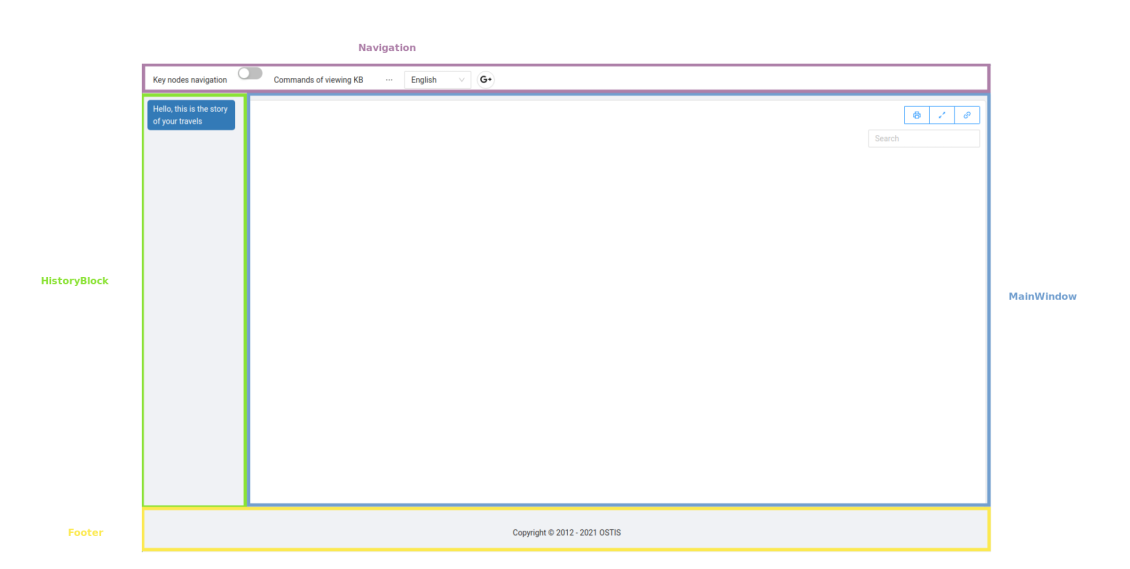
\includegraphics[width=1\linewidth]{figures/sd_ui/startPage.png}}}
\scnaddlevel{1}
\scnaddlevel{-1}
\scnrelfromset{декомпозиция}{
Панель навигации\\
	\scnaddlevel{1}
	\scniselement{неатомарный компонент пользовательского интерфейса}
	\scnrelfromset{декомпозиция}{
	Главное меню\\	
		\scnaddlevel{1}
		\scniselement{меню}
		\scnrelfromset{декомпозиция}{
		Пункт меню для навигации по ключевым понятиям\\
			\scnaddlevel{1}
			\scniselement{пункт меню}
			\scnaddlevel{-1}
		;Пункт меню для выполнения команд просмотра базы знаний\\
			\scnaddlevel{1}
			\scniselement{пункт меню}
			\scnaddlevel{-1}			
		;Компонент перехода в экспертный режим\\
			\scnaddlevel{1}
			\scniselement{переключатель}
			\scnaddlevel{-1}
	}
	\scnaddlevel{-1}
	;Компонент выбора языка\\
		\scnaddlevel{1}
		\scniselement{компонент выбора одного значения}
		\scnaddlevel{-1}
	;Компонент авторизации\\
		\scnaddlevel{1}
		\scniselement{кнопка}
		\scnaddlevel{-1}}
	\scnaddlevel{-1}
;Блок истории запросов пользователя\\
	\scnaddlevel{1}
	\scniselement{неатомарный компонент пользовательского интерфейса}
	\scnaddlevel{-1}
;Основной блок\\
	\scnaddlevel{1}
	\scniselement{неатомарный компонент пользовательского интерфейса}
	\scnrelfromset{декомпозиция}{
	Главное окно\\
		\scnaddlevel{1}
		\scniselement{окно}
		\scnaddlevel{-1}
	;Панель инструментов\\
		\scnaddlevel{1}
		\scniselement{неатомарный компонент пользовательского интерфейса}
		\scnrelfromset{декомпозиция}{Кнопка отправки содержимого главного окна на печать\\
			\scnaddlevel{1}
			\scniselement{кнопка}
			\scnaddlevel{-1}
		;Кнопка управления видимостью блока истории запросов пользователя\\
			\scnaddlevel{1}
			\scniselement{кнопка}
			\scnaddlevel{-1}
		;Кнопка отображения ссылки на текущий запрос пользователя\\
			\scnaddlevel{1}
			\scniselement{кнопка}
			\scnaddlevel{-1}
		;Поле поиска\\	
			\scnaddlevel{1}
			\scniselement{однострочное текстовое поле}
			\scnaddlevel{-1}
		}
	\scnaddlevel{-1}
	}
\scnaddlevel{-1}
;Панель отображения информации об авторских правах\\
	\scnaddlevel{1}
	\scniselement{неатомарный компонент пользовательского интерфейса}
	\scnaddlevel{-1}
}
\scnendstruct \scnendcurrentsectioncomment
\end{SCn}
\scsection{Предметная область и онтология интерфейсных действий пользователей ostis-системы}
\label{sd_user_interface_actions}
\begin{SCn}

\scnsectionheader{\currentname}

\scnstartsubstruct

\scnrelfrom{соавтор}{Садовский М.Е.}

\scnheader{Предметная область интерфейсных действий пользователей}
\scniselement{предметная область}
\scnsdmainclass{интерфейсное действие пользователя}
\scnsdclass{действие мышью;прокрутка мышью;прокрутка мышью вверх;прокрутка мышью вниз;наведение мышью;отпускание мышью;нажатие мыши;одиночное нажатие мыши;двойное нажатие мыши;жест мышью;отведение мышью;перетаскивание мышью;действие голосом;действие клавиатурой;нажатие функциональной клавиши;нажатие клавиши набора текста;действие осязанием;действие сенсором;нажатие сенсора;одиночное нажатие сенсора;двойное нажатие сенсора;жест по сенсору;жест по сенсору одним пальцем;жест по сенсору несколькими пальцами;отпускание сенсором;перетаскивание сенсором;действие пером;нажатие функциональной клавиши пером;рисование пером;написание текста пером}
\scnsdrelation{инициируемое пользовательским интерфейсом действие*}
\scnrelfrom{частная предметная область}{
	Предметная область интерфейсных действий пользователей ostis-системы
}

\scnheader{интерфейсное действие пользователя}
\scnidtf{user interface action}
\scnexplanation{Действие, выполняемое пользователем над некоторым \textit{компонентом пользовательского интерфейса}. Для связи данного действия с \textit{компонентом пользовательского интерфейса} и необходимым к выполнению \textit{внутренним действием системы} используется отношение \textit{инициируемое пользовательским интерфейсом действие*}}
	\scnsuperset{действие мышью}
	\scnaddlevel{1}
	\scnidtf{mouse-action}
	\scnaddlevel{-1}
		\scnaddlevel{1}
		\scnsuperset{прокрутка мышью}
		\scnaddlevel{1}
		\scnidtf{mouse-scroll}
		\scnaddlevel{-1}
			\scnaddlevel{1}
			\scnsuperset{прокрутка мышью вверх}
			\scnaddlevel{1}
			\scnidtf{mouse-scroll-up}
			\scnaddlevel{-1}
			\scnsuperset{прокрутка мышью вниз}
			\scnaddlevel{1}
			\scnidtf{mouse-scroll-down}
			\scnaddlevel{-1}
			\scnaddlevel{-1}
		\scnsuperset{наведение мышью}
		\scnaddlevel{1}
		\scnidtf{mouse-hover}
		\scnaddlevel{-1}
		\scnsuperset{отпускание мышью}
		\scnaddlevel{1}
		\scnidtf{mouse-drop}
		\scnaddlevel{-1}
		\scnsuperset{нажатие мыши}
		\scnaddlevel{1}
		\scnidtf{mouse-click}
		\scnaddlevel{-1}
			\scnaddlevel{1}
			\scnsuperset{одиночное нажатие мыши}
			\scnaddlevel{1}
			\scnidtf{mouse-single-click}
			\scnaddlevel{-1}
			\scnsuperset{двойное нажатие мыши}
			\scnaddlevel{1}
			\scnidtf{mouse-double-click}
			\scnaddlevel{-1}			
			\scnaddlevel{-1}
		\scnsuperset{жест мышью}
		\scnaddlevel{1}
		\scnidtf{mouse-gesture}
		\scnaddlevel{-1}
		\scnsuperset{отведение мышью}	
		\scnaddlevel{1}
		\scnidtf{mouse-unhover}
		\scnaddlevel{-1}	
		\scnsuperset{перетаскивание мышью}
		\scnaddlevel{1}
		\scnidtf{mouse-drag}
		\scnaddlevel{-1}
		\scnaddlevel{-1}		
	\scnsuperset{действие голосом}
	\scnaddlevel{1}
	\scnidtf{speech-action}
	\scnaddlevel{-1}
	\scnsuperset{действие клавиатурой}
	\scnaddlevel{1}
	\scnidtf{keyboard-action}
	\scnaddlevel{-1}
			\scnaddlevel{1}
			\scnsuperset{нажатие функциональной клавиши}
			\scnaddlevel{1}
			\scnidtf{press-function-key}
			\scnaddlevel{-1}
			\scnsuperset{нажатие клавиши набора текста}
			\scnaddlevel{1}
			\scnidtf{type-text}
			\scnaddlevel{-1}
			\scnaddlevel{-1}	
	\scnsuperset{действие осязанием}
	\scnaddlevel{1}
	\scnidtf{tangible-action}
	\scnaddlevel{-1}	
	\scnsuperset{действие сенсором}	
	\scnaddlevel{1}
	\scnidtf{touch-action}
	\scnaddlevel{-1}
		\scnaddlevel{1}
		\scnsuperset{нажатие сенсора}
		\scnaddlevel{1}
		\scnidtf{touch-click}
		\scnaddlevel{-1}
			\scnaddlevel{1}
			\scnsuperset{одиночное нажатие сенсора}
			\scnaddlevel{1}
			\scnidtf{touch-single-click}
			\scnaddlevel{-1}
			\scnsuperset{двойное нажатие сенсора}
			\scnaddlevel{1}
			\scnidtf{touch-double-click}
			\scnaddlevel{-1}
			\scnaddlevel{-1}
		\scnsuperset{жест по сенсору}
		\scnaddlevel{1}
		\scnidtf{touch-gesture}
		\scnaddlevel{-1}
			\scnaddlevel{1}
			\scnsuperset{жест по сенсору одним пальцем}
			\scnaddlevel{1}
			\scnidtf{one-fingure-gesture}
			\scnaddlevel{-1}
			\scnsuperset{жест по сенсору несколькими пальцами}
			\scnaddlevel{1}
			\scnidtf{multiple-finger-gesture}
			\scnaddlevel{-1}
			\scnaddlevel{-1}
		\scnsuperset{отпускание сенсором}
		\scnaddlevel{1}
		\scnidtf{touch-drop}
		\scnaddlevel{-1}
		\scnsuperset{перетаскивание сенсором}
		\scnaddlevel{1}
		\scnidtf{touch-drag}
		\scnaddlevel{-1}
		\scnaddlevel{-1}
	\scnsuperset{действие пером}
	\scnaddlevel{1}
	\scnidtf{pen-base-action}
	\scnaddlevel{-1}	
		\scnaddlevel{1}
		\scnsuperset{нажатие функциональной клавиши пером}
		\scnaddlevel{1}
		\scnidtf{touch-function-key}
		\scnaddlevel{-1}
		\scnsuperset{рисование пером}
		\scnaddlevel{1}
		\scnidtf{draw}
		\scnaddlevel{-1}
		\scnsuperset{написание текста пером}
		\scnaddlevel{1}
		\scnidtf{write-text}
		\scnaddlevel{-1}
		\scnaddlevel{-1}
		
		
\scnheader{прокрутка мышью}
\scnexplanation{\textit{прокрутка мышью} -- интерфейсное действие пользователя, соответствующее прокрутке содержимого некоторого компонента пользовательского интерфейса при помощи мыши.}

\scnheader{наведение мышью}
\scnexplanation{\textit{наведение мышью} -- интерфейсное действие пользователя, соответствующее появлению курсора мыши в рамках компонента пользовательского интерфейса.}

\scnheader{отпускание мышью}
\scnexplanation{\textit{отпускание мышью} -- интерфейсное действие пользователя, соответствующее отпусканию некоторого компонента пользовательского интерфейса в рамках другого компонента пользовательского интерфейса при помощи мыши.}

\scnheader{нажатие мыши}
\scnexplanation{\textit{нажатие мыши} -- интерфейсное действие пользователя, соответствующее выполнению нажатия мыши в рамках некоторого компонента пользовательского интерфейса.}

\scnheader{отведение мышью}
\scnexplanation{\textit{отведение мышью} -- интерфейсное действие пользователя, соответствующее выходу курсора мыши за рамки компонента пользовательского интерфейса.}

\scnheader{перетаскивание мышью}
\scnexplanation{\textit{перетаскивание мышью} -- интерфейсное действие пользователя, соответствующее перетаскиванию компонента пользовательского интерфейса при помощи мыши.}

\scnheader{нажатие сенсора}
\scnexplanation{\textit{нажатие сенсора} -- интерфейсное действие пользователя, соответствующее выполнению нажатия сенсора в рамках некоторого компонента пользовательского интерфейса.}

\scnheader{жест по сенсору}
\scnexplanation{\textit{жест по сенсору} -- интерфейсное действие пользователя, соответствующее выполнению некоторого жеста, выполняемого при помощи движения пальцев на экране сенсора.}

\scnheader{отпускание сенсором}
\scnexplanation{\textit{отпускание сенсором} -- интерфейсное действие пользователя, соответствующее отпусканию некоторого компонента пользовательского интерфейса в рамках другого компонента пользовательского интерфейса при помощи сенсора.}

\scnheader{перетаскивание сенсором}
\scnexplanation{\textit{перетаскивание сенсором} -- интерфейсное действие пользователя, соответствующее перетаскиванию компонента пользовательского интерфейса при помощи сенсора.}

\scnheader{действие пером}
\scnexplanation{\textit{действие пером} -- интерфейсное действие пользователя, осуществляемое при помощи пера на графическом планшете.}

\scnheader{класс интерфейсных действий пользователя}
\scnsubset{класс действий}
\scnrelto{семейство подмножеств}{интерфейсное действие пользователя}
\scnexplanation{\textit{класс интерфейсных действий пользователя} -- множество, элементами которого являются классы \textit{интерфейсных действий пользователя}.}

\scnheader{инициируемое пользовательским интерфейсом действие*}
\scnexplanation{При взаимодействии пользователя с \textit{компонентом пользовательского интерфейса} могут быть произведены различные интерфейсные действия. В зависимости от выполненного интерфейсного действия и компонента, над которым оно было выполнено, происходит инициирование некоторого \textit{внутреннего действия системы}. Для задания такого инициируемого при взаимодействии с пользовательским интерфейсом действия и используется указанное отношение. Первым компонентом связки отношения \textit{инициируемое пользовательским интерфейсом действие*} является связка, элементами которой являются элемент множества компонентов пользовательского интерфейса и и элемент множества \textit{класс интерфейсных действий пользователя}. Вторым компонентом является элемент множества \textit{класс внутренних действий системы}.}
\scniselement{квазибинарное отношение}
\scniselement{ориентированное отношение}
\scnaddhind{1}
\scnrelfrom{первый домен}{компонент пользовательского интерфейса $\cup$ класс интерфейсных действий пользователя}
\scnrelfrom{второй домен}{класс внутренних действий системы}
\scnrelfrom{описание примера}{
	\scnfilescg{figures/sd_ui/ui_initiated_action.png}}}

\bigskip
\scnendstruct \scnendcurrentsectioncomment

\end{SCn}
\scsection{Предметная область и онтология действий и внутренних агентов пользовательского интерфейса ostis-системы}
\scsection{Предметная область и онтология естественных языков}
\label{sec:sd_natural_languages}
\begin{SCn}

\scnsectionheader{\currentname}

\scnstartsubstruct

\scnheader{Предметная область естественных языков}
\scniselement{предметная область}
\scnsdmainclasssingle{язык}
\scnsdclass{плановый язык;язык общения;лексема;номинативная единица;комбинаторный вариант лексемы;естественный язык;тайген;ёген}
\scnsdrelation{морфологическая парадигма*;член предложения\scnrolesign }

\scnheader{язык}
\scnsubdividing{естественный язык\\
	\scnaddlevel{1}
	\scnexplanation{Естественный язык представляет собой язык, который не был создан целенаправленно}
	\scnaddlevel{-1}
;искусственный язык\\
	\scnaddlevel{1}
	\scnexplanation{Искусственный язык представляет собой язык, специально разработанный для достижения определённых целей}
	\scnhaselement{Эсперанто}
	\scnhaselement{Python}
	\scnsuperset{сконструированный язык}
	\scnaddlevel{1}
	\scnexplanation{Сконструированный язык представляет собой искусственный язык, предназначенный для общения людей}
	\scnhaselement{Эсперанто}
	\scnaddlevel{-1}
	\scnaddlevel{-1}
}
\scnsuperset{международный язык}
	\scnaddlevel{1}
	\scnexplanation{Международный язык представляет собой естественный или искусственный язык, использующийся для общения людей разных из стран}
	\scnhaselement{Английский язык}
	\scnhaselement{Русский язык}
	\scnaddlevel{-1}

\scnheader{плановый язык}
\scnreltoset{пересечение}{сконструированный язык;международный язык}

\scnheader{язык общения}
\scnreltoset{объединение}{естественный язык;сконструированный язык}
\scnhaselement{Английский язык}
\scnhaselement{Русский язык}
\scnhaselement{Эсперанто}
\scnreltoset{объединение}{корневой язык\\
	\scnaddlevel{1}
	\scnexplanation{Корневой язык представляет собой язык, для которого характерно полное отсутствие словоизменения и наличие грамматической значимости порядка слов, состоящих только из корня.}
	\scnhaselement{Английский язык}
	\scnaddlevel{-1}
;агглютинативный язык\\
	\scnaddlevel{1}
	\scnexplanation{Агглютинативный язык характеризуется развитой системой употребления суффиксов, приставок, добавляемых к неизменяемой основе слова, которые используются для выражения категорий числа, падежа, рода и др.}
	\scnhaselement{Английский язык}
	\scnaddlevel{-1}
;флективный язык\\
	\scnaddlevel{1}
	\scnexplanation{Для флективного языка характерно развитое употребление окончаний для выражения категорий рода, числа, падежа, сложная система склонения глаголов, чередование гласных в корне, а также строгое различение частей речи.}
	\scnhaselement{Русский язык}
	\scnaddlevel{-1}
;профлективный язык\\
	\scnaddlevel{1}
	\scnexplanation{Для профлективного языка характерны агглютинация (в случае именного словоизменения), флексия и чередование гласных (аблаут)(в случае глагольного словоизменения).}
	\scnaddlevel{-1}
}

\scnheader{лексема}
\scnsubset{файл}
\scnexplanation{\textit{Лексема} -- тайген или ёген конкретного естественного языка.}
	\scnaddlevel{1}
	\scnrelfrom{источник}{\scncite{Hardzei2005}}
	\scnaddlevel{-1}
	
\scnheader{номинативная единица}
\scnsubset{файл}
\scnexplanation{\textit{Номинативная единица} -- устойчивая последовательность комбинáторных вариантов лексем, в которой один вариант лексемы (модификатор) определяет другой (актуализатор), например: ‘записная книжка’, ‘бежать галопом’.}
	\scnaddlevel{1}
	\scnrelfrom{источник}{\scncite{Hardzei2005}}
	\scnaddlevel{-1}
	
\scnheader{комбинаторный вариант лексемы}
\scnsubset{файл}
\scnexplanation{\textit{Комбинáторный вариант лексемы } -- вариант лексемы в упорядоченном наборе её вариантов (парадигме).}
	\scnaddlevel{1}
	\scnrelfrom{источник}{\scncite{Hardzei2007}}
	\scnaddlevel{-1}


\scnheader{морфологическая парадигма*}
\scniselement{квазибинарное отношение}
\scnexplanation{\textit{Морфологическая парадигма*} -- квазибинарное отношение, связывающее лексему с её комбинáторными вариантами.}
\scnrelfrom{первый домен}{словоформа}
\scnrelfrom{второй домен}{лексема}

\scnheader{естественный язык}
\scnsubdividing{
	часть языка\\
	\scnaddlevel{1}
	\scnsubdividing{тайген;ёген}
	\scnaddlevel{-1}
	;знак алфавита синтаксиса\\
		\scnaddlevel{1}
		\scnexplanation{\textit{Знаки алфавита синтаксиса} -- вспомогательные средства синтаксиса (на макроуровне -- предлоги, послелоги, союзы, частицы и др., на микроуровне -- флексии, префиксы, постфиксы, инфиксы и др.), служащие для соединения составных частей языковых структур и образования морфологических парадигм.}
			\scnaddlevel{1}
			\scnrelfrom{источник}{\scncite{Hardzei2005}}
			\scnaddlevel{-1}
		\scnaddlevel{-1}
}

\scnheader{тайген}
\scnexplanation{\textit{Тайген} -- часть языка, обозначающая индивида.}
	\scnaddlevel{1}
	\scnrelfrom{источник}{\scncite{Hardzei2006}}
	\scnrelfrom{источник}{\scncite{Hardzei2015}}
	\scnaddlevel{-1}
\scnsubdividing{
	развёрнутый тайген\\
	\scnaddlevel{1}
	\scnsubdividing{
		составной тайген\\
		;сложный тайген\\
	}   
	\scnaddlevel{-1}
	;свёрнутый тайген\\
	\scnaddlevel{1}
	\scnsubdividing{
		сокращённый тайген\\
		;сжатый тайген\\
			\scnaddlevel{1}
			\scnsubdividing{
				информационный тайген\\
				\scnaddlevel{1}
				\scnexplanation{\textit{Информационный тайген} -- тайген, обозначающий индивида в информационном фрагменте модели мира.}
					\scnaddlevel{1}
					\scnrelfrom{источник}{\scncite{Hardzei2006}}
					\scnrelfrom{источник}{\scncite{Hardzei2015}}
					\scnaddlevel{-1}
				\scnaddlevel{-1}
				;физический тайген\\
				\scnaddlevel{1}
				\scnexplanation{\textit{Физический тайген} -- тайген, обозначающий индивида в физическом фрагменте модели мира. }
					\scnaddlevel{1}
					\scnrelfrom{источник}{\scncite{Hardzei2006}}
					\scnrelfrom{источник}{\scncite{Hardzei2015}}
					\scnaddlevel{-1}
				\scnsubdividing{
					постоянный тайген\\
					\scnaddlevel{1}
					\scnexplanation{\textit{Постоянный тайген} -- физический тайген, обозначающий постоянного индивида.}
						\scnaddlevel{1}
						\scnrelfrom{источник}{\scncite{Hardzei2006}}
						\scnrelfrom{источник}{\scncite{Hardzei2015}}
						\scnaddlevel{-1}
					\scnaddlevel{-1}
					;переменный тайген\\
					\scnaddlevel{1}
					\scnexplanation{\textit{Переменный тайген} -- физический тайген, обозначающий переменного индивида.}
						\scnaddlevel{1}
						\scnrelfrom{источник}{\scncite{Hardzei2006}}
						\scnrelfrom{источник}{\scncite{Hardzei2015}}
						\scnaddlevel{-1}
					\scnaddlevel{-1}
				}
				\scnsubdividing{
					качественный тайген
					;количественный тайген\\
				}
				\scnsubdividing{
					одноместный тайген
					;многоместный тайген\\
					\scnaddlevel{1}
					\scnsuperset{интенсивный тайген}
					\scnsuperset{экстенсивный тайген}
					\scnaddlevel{-1}	
				}
			}
			\scnaddlevel{-1}
	}
	\scnaddlevel{-1}
}
\scnaddlevel{-1}	

\scnheader{ёген}
\scnexplanation{\textit{Ёген} -- часть языка, обозначающая признак индивида.}
	\scnaddlevel{1}
	\scnrelfrom{источник}{\scncite{Hardzei2006}}
	\scnrelfrom{источник}{\scncite{Hardzei2015}}
	\scnaddlevel{-1}
\scnsubdividing{
	развёрнутый ёген\\
	\scnaddlevel{1}
	\scnsubdividing{
		составной ёген
		;сложный ёген
	}
	\scnaddlevel{-1}
	;свёрнутый ёген\\
	\scnaddlevel{1}
	\scnsubdividing{
		сокращённый ёген\\
			\scnaddlevel{1}
			\scnsubdividing{
				информационный ёген\\
					\scnaddlevel{1}
					\scnexplanation{\textit{Информационный ёген} -- еген, обозначающий признак индивида в информационном фрагменте модели мира.}
						\scnaddlevel{1}
						\scnrelfrom{источник}{\scncite{Hardzei2006}}
						\scnrelfrom{источник}{\scncite{Hardzei2007a}}
						\scnaddlevel{-1}
					\scnaddlevel{-1}
				;физический ёген\\
				\scnaddlevel{1}
				\scnexplanation{\textit{Физический ёген} -- еген, обозначающий признак индивида в физическом фрагменте модели мира.}
					\scnaddlevel{1}
					\scnrelfrom{источник}{\scncite{Hardzei2006}}
					\scnrelfrom{источник}{\scncite{Hardzei2007a}}
					\scnaddlevel{-1}
				\scnsubdividing{
					постоянный ёген\\
						\scnaddlevel{1}
						\scnexplanation{\textit{Постоянный ёген} - физический ёген, обозначающий постоянный признак индивида.}
							\scnaddlevel{1}
							\scnrelfrom{источник}{\scncite{Hardzei2006}}
							\scnrelfrom{источник}{\scncite{Hardzei2007a}}
							\scnaddlevel{-1}
						\scnaddlevel{-1}
					;переменный ёген\\
						\scnaddlevel{1}
						\scnexplanation{\textit{Переменный ёген} -- физический ёген, обозначающий переменный признак индивида.}
							\scnaddlevel{1}
							\scnrelfrom{источник}{\scncite{Hardzei2006}}
							\scnrelfrom{источник}{\scncite{Hardzei2007a}}
							\scnaddlevel{-1}
						\scnaddlevel{-1}
				}
				\scnsubdividing{
					качественный ёген
					;количественный ёген
				}
				\scnsubdividing{
					одноместный ёген
					;многоместный ёген\\
						\scnaddlevel{1}
						\scnsubdividing{
							интенсивный ёген
							;экстенсивный ёген
						}
						\scnaddlevel{-1}
				}
				\scnaddlevel{-1}
			}
			\scnaddlevel{-1}
		;сжатый ёген
	}
	\scnaddlevel{-1}
}

\scnheader{Пример sc.g-текста, описывающего лексему}
\scneqscg{figures/sd_natural_languages/lexeme_example.png}
\scniselement{sc.g-текст}
\scnexplanation{Здесь представлено описание лексемы, содержащее указание ее принадлежности определённой части речи. Также описание содержит морфологическую парадигму данной лексемы, связывающую ее с ее словоформами.}

\scnheader{член предложения\scnrolesign}
\scniselement{ролевое отношение}
\scnexplanation{\textit{Член предложения\scnrolesign} -- это отношение, связывающее декомпозицию текста с файлом, содержимое которого (часть языка) играет в декомпозируемом тексте определенную синтаксическую роль.}
	\scnaddlevel{1}
	\scnrelfrom{источник}{\scncite{Hardzei2005}}
	\scnaddlevel{-1}
\scnsubdividing{
	главный член предложения\scnrolesign\\
	\scnaddlevel{1}
	\scnsubdividing{
		подлежащее\scnrolesign\\
			\scnaddlevel{1}
			\scnexplanation{\textit{Подлежащее\scnrolesign} -- это одно из главных ролевых отношений, связывающее декомпозицию текста с файлом, содержимое которого обозначает исходный пункт описания события, выбранный наблюдателем. }
				\scnaddlevel{1}
				\scnrelfrom{источник}{\scncite{Hardzei2020}}
				\scnaddlevel{-1}
			\scnaddlevel{-1}
		;сказуемое\scnrolesign\\
			\scnaddlevel{1}
			\scnexplanation{\textit{Сказуемое\scnrolesign} -- это одно из главных ролевых отношений, связывающее декомпозицию текста с файлом, содержимое которого обозначает отображение наблюдателем исходного пункта описания события в конечный.}
				\scnaddlevel{1}
				\scnrelfrom{источник}{\scncite{Hardzei2020}}
				\scnaddlevel{-1}
			\scnaddlevel{-1}
		;прямое дополнение\scnrolesign\\
			\scnaddlevel{1}
			\scnexplanation{\textit{Прямое дополнение\scnrolesign} -- это одно из главных ролевых отношений, связывающее декомпозицию текста с файлом, содержимое которого обозначает конечный пункт описания события, выбранный наблюдателем.}
				\scnaddlevel{1}
				\scnrelfrom{источник}{\scncite{Hardzei2020}}
				\scnaddlevel{-1}
			\scnaddlevel{-1}
	}
	\scnaddlevel{-1}
	;второстепенный член предложения\scnrolesign\\
	\scnaddlevel{1}
	\scnsubdividing{
		косвенное дополнение\scnrolesign
		;определение\scnrolesign\\
			\scnaddlevel{1}
			\scnexplanation{\textit{Определение\scnrolesign} -- это одно из второстепенных ролевых отношений, связывающее декомпозицию текста с файлом, содержимое которого обозначает модификацию подлежащего, дополнения, обстоятельства места и времени.}
				\scnaddlevel{1}
				\scnrelfrom{источник}{\scncite{Hardzei2007a}}
				\scnrelfrom{источник}{\scncite{Hardzei2017a}}
				\scnrelfrom{источник}{\scncite{Hardzei2007b}}
				\scnaddlevel{-1}
			\scnaddlevel{-1}
		;обстоятельство\scnrolesign\\
			\scnaddlevel{1}
			\scnexplanation{\textit{Обстоятельство\scnrolesign} -- это одно из второстепенных ролевых отношений, связывающее декомпозицию текста с файлом, содержимое которого обозначает либо модификацию, либо локализацию сказуемого.}
				\scnaddlevel{1}
				\scnrelfrom{источник}{\scncite{Hardzei2007a}}
				\scnrelfrom{источник}{\scncite{Hardzei2017a}}
				\scnrelfrom{источник}{\scncite{Hardzei2007b}}
				\scnaddlevel{-1}
			\scnsubdividing{
				обстоятельство степени\scnrolesign\\
					\scnaddlevel{1}
					\scnexplanation{Обстоятельство степени -- обстоятельство, обозначающее модификацию сказуемого.}
					\scnaddlevel{-1}
				;обстоятельство образа действия\scnrolesign\\
					\scnaddlevel{1}
					\scnexplanation{Обстоятельство образа действия -- обстоятельство, обозначающее модификацию сказуемого.}
					\scnaddlevel{-1}
				;обстоятельство места\scnrolesign\\
				\scnaddlevel{1}
				\scnexplanation{Обстоятельства места -- обстоятельство, обозначающее пространственную локализацию сказуемого.}
				\scnsubdividing{
					динамическое обстоятельство места\scnrolesign;
					статическое обстоятельство места\scnrolesign
				}
				\scnaddlevel{-1}
				;обстоятельство времени\scnrolesign\\
				\scnaddlevel{1}
				\scnexplanation{Обстоятельство времени -- обстоятельство, обозначающее временную локализацию сказуемого.}
				\scnsubdividing{
					динамическое обстоятельство времени\scnrolesign;
					статическое обстоятельство времени\scnrolesign
				}
				\scnaddlevel{-1}
			}
			\scnaddlevel{-1}
	}
	\scnaddlevel{-1}
}

\scnheader{Пример этапов разбора текста естественного языка}

\scnstartsubstruct
	\scnaddlevel{1}
	\scnfilescg{figures/sd_natural_languages/nl_text.png}
	\scnexplanation{с точки зрения ostis-системы, любой естественно-языкой текст является \textit{файлом.}}
	\scnrelfrom{лексическая структура}{\scnfilescg{figures/sd_natural_languages/nl_lexical.png}}
		\scnaddlevel{1}
		\scnexplanation{Данная конструкция включает в себя декомпозицию исходного текста на фрагменты, а также указание принадлежности данных фрагментов определённой \textit{лексеме}, \textit{номинативной единице} или \textit{знаку алфавита синтаксиса}.}
		\scnrelfrom{синтаксическая структура}{\scnfilescg{figures/sd_natural_languages/nl_synactical.png}}
			\scnaddlevel{1}
			\scnexplanation{Здесь приведена только частью синтаксической структуры. Оставшаяся часть записывается аналогично.}
			\scnaddlevel{-1}
		\scnaddlevel{-1}
	\scnaddlevel{-1}
\scnendstruct

\bigskip
\scnendstruct \scnendcurrentsectioncomment

\end{SCn}

\scchapter{\textbf{Предметная область и онтология базовых интерпретаторов логико-семантических моделей ostis-систем}}
\label{sd_interpreters}
\begin{SCn}

\scnsectionheader{\currentname}
\scnstartsubstruct

\scnidtf{Предметная область и онтология платформ интерпретации sc-моделей компьютерных систем}
\scniselement{раздел базы знаний}
\scnrelfromlist{дочерний раздел}{\nameref{sd_program_interp};\nameref{sd_sem_comp}}

\scnheader{Предметная область базовых интерпретаторов логико-семантических моделей ostis-систем}
\scniselement{предметная область}
\scnsdmainclasssingle{платформа интерпретации sc-моделей компьютерный систем}
%\scnsdclass{***}
%\scnsdrelation{***}

\scnheader{логико-семантическая модель кибернетической системы}
\scnidtf{формальная модель (формальное описание) функционирования кибернетической системы, состоящая из:
	\begin{scnitemize}
		\item формальной модели информации, хранимой в памяти кибернетической системы;
		\item формальной модели коллектива агентов, осуществляющих обработку указанной информации.
\end{scnitemize}}
\scnsuperset{sc-модель кибернетической системы}
\scnaddlevel{1}
\scnidtf{логико-семантическая модель кибернетической системы, представленная в SC-коде}
\scnidtf{логико-семантическая модель ostis-системы, которая, в частности, может быть функционально эквивалентной моделью какой-либо кибернетической системы, не являющейся ostis-системой}
\scnaddlevel{-1}

\scnheader{кибернетическая система}
\scnsuperset{компьютерная система}
\scnaddlevel{1}
\scnidtf{искусственная кибернетическая система}
\scnsuperset ostis-система}
\scnaddlevel{1}
\scnidtf{компьютерная система, построенная по технологии OSTIS на основе интерпретации спроектированной логико-семантическая sc-модель этой системы}
\scnaddlevel{-2}

\scnheader{платформа интерпретации sc-моделей компьютерных систем}
\scnidtf{базовый интерпретатор логико-семантических моделей ostis-систем}
\scnidtf{Семейство платформ интерпретации sc-моделей компьютерных систем}
\scnidtf{платформа реализации sc-моделей компьютерных систем}
\scnidtftext{часто используемый sc-идентификатор}{универсальный интерпретатор sc-моделей компьютерных систем}
\scnidtf{универсальный интерпретатор унифицированных логико-семантических моделей компьютерных систем}
\scnsubset{встроенная ostis-система}
\scnidtf{встроенная пустая ostis-система}
\scnidtf{универсальный интерпретатор sc-моделей ostis-систем}
\scnidtf{универсальная базовая ostis-система, обеспечивающая имитацию любой ostis-системы путем интерпретации sc-модели имитируемой ostis-системы}
\scnnote{соотношение между имитируемой и универсальной ostis-системой в известной мере аналогично соотношению между машиной Тьюринга и универсальной машиной Тьюринга}
\scnexplanation{Под \textbf{\textit{платформой интерпретации sc-моделей компьютерных систем}} понимается реализация платформы интерпретации sc-моделей, которая в общем случае включает в себя:

Реализация \textit{платформы интерпретации sc-моделей компьютерных систем} (\textit{универсального интерпретатора sc-моделей компьютерных систем}) может иметь большое число вариантов -- как программно, так и аппаратно реализованных. Логическая архитектура \textit{платформы интерпретации sc-моделей компьютерных систем} обеспечивает независимость проектируемых компьютерных систем от многообразия вариантов реализации интерпретатора их моделей и в общем случае включает в себя:

\begin{scnitemize}
    \item хранилище \textit{sc-текстов} (\textit{sc-хранилище}, хранилище знаковых конструкций, представленных SC-коде);
    \item файловую память \textit{sc-машины};
    \item средства, обеспечивающие взаимодействие \textit{sc-агентов} над общей памятью (sc-памятью);
    \item базовые средства интерфейса для взаимодействия системы с внешним миром (пользователем или другими системами). Указанные средства включают в себя, как минимум, редактор, транслятор (в sc-память и из нее) и визуализатор для одного из базовых универсальных вариантов представления \textit{SC-кода} (\textit{SCg-код}, \textit{SCs-код}, \textit{SCn-код}), средства, позволяющие задавать системе вопросы из некоторого универсального класса (например, запрос семантической окрестности некоторого объекта);
    \item реализацию \textit{Абстрактной scp-машины}, то есть интерпретатор \textit{scp-программ} (программ Языка SCP).
\end{scnitemize}
При необходимости, в \textbf{\textit{платформу интерпретации sc-моделей компьютерных систем}} могут быть заранее на платформенно-зависимом уровне включены какие-либо компоненты машин обработки знаний или баз знаний, например, с целью упрощения создания первой версии \textit{прикладной ostis-системы}.

Реализация платформы может осуществляться на основе произвольного набора существующих технологий, включая аппаратную реализацию каких-либо ее частей. С точки зрения компонентного подхода любая \textbf{\textit{платформа интерпретации sc-моделей компьютерных систем}} является \textbf{\textit{платформенно-зависимым многократно используемым компонентом}}.}
\scnsuperset{программный вариант реализации платформы интерпретации sc-моделей компьютерных систем}
\scnsuperset{семантический ассоциативный компьютер}
\scnsubdividing{однопользовательский вариант реализации платформы интерпретации sc-моделей компьютерных систем\\
	\scnaddlevel{1}
		\scnidtf{вариант реализации платформы интерпретации sc-моделей компьютерных систем, рассчитанный на то, что с конкретной ostis-системой взаимодействует только один пользователь (владелец)}
		\scnnote{При таком варианте реализации платформы оказывается невозможным реализовать некоторые важные принципы \textit{Технологии OSTIS}, например, коллективную согласованную разработку базы знаний системы в процессе ее эксплуатации. При этом могут использоваться различные сторонние средства, например для разработки базы знаний на уровне исходных текстов.}
	\scnaddlevel{-1}
;многопользовательский вариант реализации платформы интерпретации sc-моделей компьютерных систем\\
\scnaddlevel{1}
	\scnidtf{вариант реализации платформы интерпретации sc-моделей компьютерных систем, рассчитанный на то, что с конкретной ostis-системой одновременно или в разное время могут взаимодействовать разные пользователи, в общем случае обладающие разными правами, сферами ответственности, уровнем опыта, и имеющие свою конфиденциальную часть хранимой в базе знаний информации}
\scnaddlevel{-1}}

\scnheader{платформа интерпретации sc-моделей компьютерных систем}
\scnsubdividing{программный вариант реализации платформы интерпретации sc-моделей компьютерных систем\\
	\scnaddlevel{1}
	\scnidtf{программная платформа интерпретации sc-моделей ostis-систем}
	\scnidtf{программный базовый интерпретатор sc-моделей ostis-систем}
	\scnaddlevel{-1}
	;семантический ассоциативный компьютер
	\scnaddlevel{1}
	\scnidtf{аппаратная платформа интерпретации sc-моделей ostis-систем}
	\scnidtf{аппаратно реализованный базовый интерпретатор sc-моделей ostis-систем}
	\scnaddlevel{-1}
}

\newpage

\scnfragmentheader{Классификация sc-элементов, на основе которой осуществляется синтаксическая спецификация sc-элементов}
\scnstartsubstruct

\scnheader{синтаксическая классификация sc-элемента}
\scnexplanation{При реализации \textit{sc-памяти} \scnbigspace \textit{синтаксическая спецификация sc-элементов}, хранимых в этой памяти, (т.е. \textit{спецификация sc-элементов}, реализуемая не средствами \textit{SC-кода}, а синтаксическим способом, неявно), осуществляется путем приписывания каждому хранимому \textit{sc-элементу} вектора значений \uline{унифицированного набора признаков}. Каждый из этих признаков характеризует принадлежность или непринадлежность специфицируемого \textit{sc-элемента} некоторому конкретному \textit{классу sc-элементов}. Очень важно задать такое семейство указанных \textit{классов sc-элементов}, которое
\begin{scnitemize}
	\item было бы достаточно компактным;
	\item обеспечивало бы достаточно высокую производительность при обработке sc-конструкций.
\end{scnitemize}

Ниже приведена классификация \textit{sc-элементов}, позволяющая выделить такое семейство \textit{классов sc-элементов}, состоящее из 34-х классов (типов) sc-элементов.

Синтаксически \textit{sc-ребром} можно считать \textit{sc-элемент}, принадлежащий следующему классу:

(\textit{обозначение пары, у которой известны оба ее компонента}
$\cap$ \textit{обозначение пары, которая не является компонентом другой пары} $\cap$ (\textit{обозначение неориентированной пары} $\cup$ \textit{обозначение пары, о которой не известно, является она ориентированной или неориентированной} $\cup$ \textit{обозначение ориентированной пары неизвестной направленности})).

При этом \textit{sc-ребро} формально можно представить либо в виде \textit{sc-дуги}, направленность которой игнорируется и, следовательно, может быть \uline{произвольной}(!), либо в виде \textit{sc-узла}, из которого явно выходят \textit{sc-дуги}, являющиеся \textit{обозначениями пар инцидентности}, которые связывают \textit{sc-ребро} с его компонентами (т.е. с \textit{sc-элементами}, соединяемыми этим \textit{sc-ребром}).

Синтаксически sc-дугой следует считать sc-элемент, который принадлежит классу (\textit{обозначение пары, у которой известны оба ее компонента} $\cap$ \textit{обозначение пары, которая не является компонентом другой пары} $\cap$ \textit{обозначение ориентированной пары известной направленности}).

Все остальные \textit{sc-элементы} с синтаксической точки зрения следует считать \textit{sc-узлами}.}

\scnheader{sc-элемент}
\scnsubdividing{sc-переменная\\
	\scnaddlevel{1}
		\scnsubdividing{sc-переменная, каждое значение которой является sc-константой;sc-переменная, каждое значение которой является sc-переменной;sc-переменная, во множество возможных значений которой входят как sc-константы, так и sc-переменные;sc-переменная, характер множества возможных значений которой не известен}
	\scnaddlevel{-1}
	;sc-константа;sc-элемент, константность или переменность которого не известна}
\scnsubdividing{обозначение временной сущности;обозначение постоянной сущности;обозначение сущности, временность или постоянство которой либо не известны, либо принципиально не могут быть установлены}
\scnsubdividing{логически удаленный sc-элемент\\
	\scnaddlevel{1}
		\scnidtf{прошлый sc-элемент}
	\scnaddlevel{-1};
	sc-элемент, логически присутствующий в текущий момент
	\scnaddlevel{1}
		\scnidtf{настоящий sc-элемент}
	\scnaddlevel{-1}
}
\scnsubdividing{обозначение файла ostis-системы;обозначение терминальной сущности, не являющейся файлом ostis-системы;обозначение множества всех синтаксически эквивалентных файлов заданной структуры\\
	\scnaddlevel{1}
		\scnidtf{обозначение всевозможных копий файла заданной структуры}
	\scnaddlevel{-1}
	;обозначение сущности, принадлежность которой классу множеств/терминальных сущностей/файлов ostis-системы не установлена;обозначение множества, которое не является множеством всех синтаксически эквивалентных файлов заданной структуры, хранимых в памяти ostis-системы\\
	\scnaddlevel{1}
		\scnsubdividing{обозначение множества, которое не является множеством всех синтаксически эквивалентных файлов заданной структуры и не является парой;обозначение множества, о котором не известно, является оно парой или нет;обозначение пары\\
		\scnaddlevel{1}
			\scnidtf{обозначение множества, мощность которого равна двум}
			\scnsubdividing{обозначение пары, у которой известны об ее компонента;обозначение пары, у которой неизвестен один ее компонент;обозначение пары, у которой неизвестны оба ее компонента}
			\scnsubdividing{обозначение пары, которая не является компонентом другой пары;обозначение пары, которая является компонентом другой пары}
			\scnsubdividing{обозначение неориентированной пары;обозначение пары, о которой не известно, является она ориентированной или нет;обозначение ориентированной пары\\
			\scnaddlevel{1}	
				\scnsubdividing{обозначение ориентированной пары известной направленности;обозначение ориентированной пары неизвестной направленности}
				\scnsubdividing{обозначение ориентированной пары, не являющейся парой принадлежности;обозначение ориентированной пары, о которой не известно, является ли она парой принадлежности или нет;обозначение пары принадлежности\\
				\scnaddlevel{1}	
					\scnsubdividing{обозначение позитивной пары принадлежности;обозначение негативной пары принадлежности;обозначение нечеткой пары принадлежности}
					\scnsubdividing{обозначение пары принадлежности, которая не является парой инцидентности, явно связывающей обозначение некоторой другой пары с одним из ее компонентов;обозначение пары инцидентности, явно связывающей обозначение некоторой ориентированной пары со вторым компонентом этой пары;обозначение пары инцидентности, явно связывающей либо обозначение некоторой ориентированной пары с первым компонентом этой пары, либо обозначение неориентированной пары с одним из ее компонентов}
				\scnaddlevel{-1}		
				}
			\scnaddlevel{-1}	
			}
		\scnaddlevel{-1}
		}
	\scnaddlevel{-1}}

\scnendstruct

\bigskip

\scnendstruct \scnendcurrentsectioncomment

\end{SCn}

\scsection{Предметная область и онтология программных вариантов реализации базового интерпретатора логико-семантических моделей ostis-систем на современных компьютерах}
\label{sd_program_interp}
\begin{SCn}
	
\scnsectionheader{\currentname}
\scnstartsubstruct

\scnheader{программный вариант реализации платформы интерпретации sc-моделей компьютерных систем}
\scnidtf{программный вариант реализации базового интерпретатора логико-семантических моделей компьютерных систем}
\scnidtf{вариант реализации базового интерпретатора логико-семантических моделей компьютерных систем на традиционных компьютерах с архитектурой фон Неймана}
\scnsuperset{web-ориентированный вариант реализации платформы интерпретации sc-моделей компьютерных систем}
\scnaddlevel{1}
	\scnidtf{вариант реализации платформы интерпретации sc-моделей компьютерных систем предполагающий взаимодействие пользователей с системой посредством сети Интернет}
	\scnsubset{многопользовательский вариант реализации платформы интерпретации sc-моделей компьютерных систем}
	\scnhaselement{Программный вариант реализации платформы интерпретации sc-моделей компьютерных систем}
\scnaddlevel{-1}

\scnheader{Программный вариант реализации платформы интерпретации sc-моделей компьютерных систем}
\scnrelfromset{декомпозиция программной системы}{Реализация sc-памяти;Реализация интерпретатора sc-моделей пользовательских интерфейсов}
\scnexplanation{Текущий \textit{Программный вариант реализации платформы интерпретации sc-моделей компьютерных систем} является web-ориентированным, то есть с точки зрения современной архитектуры каждая ostis-система представляет собой web-сайт доступный онлайн посредством обычного браузера. Такой вариант реализации обладает очевидным преимуществом -- доступ к системе возможен из любой точки мира, где есть Интернет, при этом для работы с системой не требуется никакого специализированного программного обеспечения. С другой стороны, такой вариант реализации обеспечивает возможность параллельной работы с системой нескольких пользователей.

В то же время, взаимодействие клиентской и серверной части организовано таким образом, что web-интерфейс может быть легко заменен на настольный или мобильный интерфейс, как универсальный, так и специализированный.

Данный вариант реализации распространяется под open-source лицензией, для хранения исходных текстов используется хостинг Github и коллективная учетная запись ostis-dev.

Реализация является кроссплатформенной и может быть собрана под ОС семейства Windows и Linux.
}
\scnrelfrom{иллюстрация}{\scnfileimage{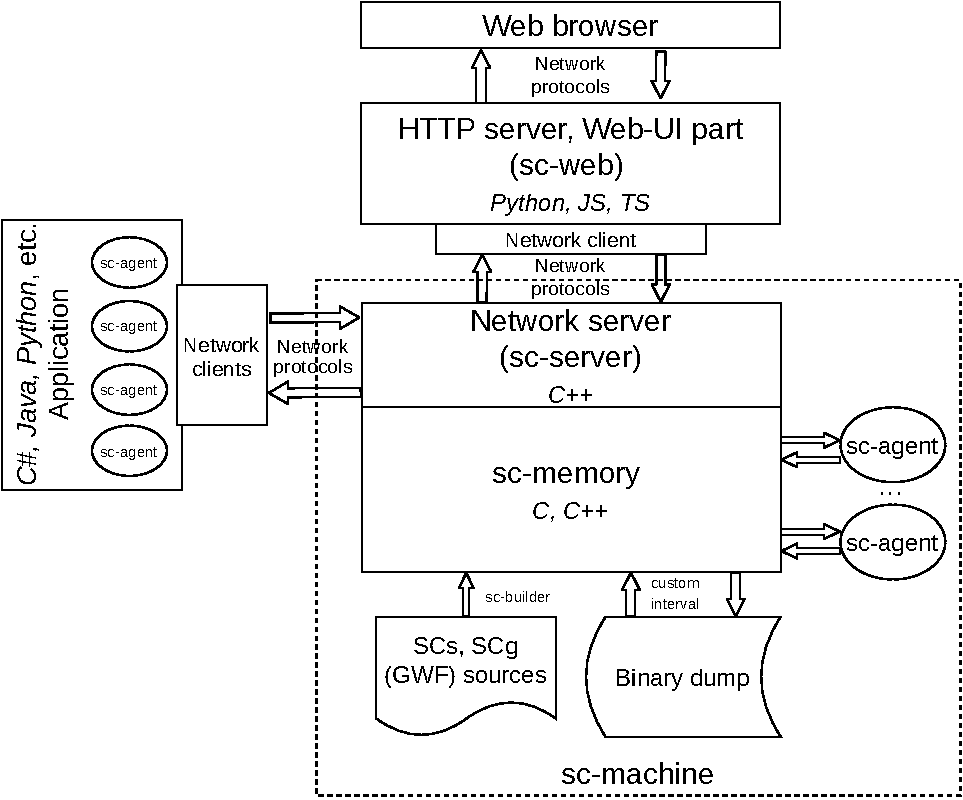
\includegraphics{figures/sd_interpreters/platform-ostis-architecture.pdf}}}
\scnaddlevel{1}
	\scnexplanation{На приведенной иллюстрации видно, что ядром платформы является \textit{Реализация sc-памяти}, с которой одновременно может взаимодействовать как с \textit{Реализацией интерпретатора sc-моделей пользовательских интерфейсов} (sc-web), так и с любыми сторонними приложениями по протоколу \textit{SCTP} или \textit{Протоколу взаимодействия с sc-памятью на основе JSON}.}
\scnaddlevel{-1}

\scnheader{Реализация sc-памяти}
\scnidtf{sc-machine}
\scntext{основной репозиторий исходных текстов}{https://github.com/ostis-dev/sc-machine.git}
\scnrelfromlist{компонент программной системы}{Реализация sc-хранилища и механизма доступа к нему;Реализация базового набора платформенно-зависимых sc-агентов и их общих компонентов;Реализация подсистемы взаимодействия с внешней средой с использованием протокола SCTP;Реализация подсистемы взаимодействия с внешней средой с использованием протоколов на основе формата JSON;Реализация вспомогательных инструментальных средств в рамках реализации sc-памяти;Реализация scp-интерпретатора}
\scntext{программная документация}{http://ostis-dev.github.io/sc-machine/}
\scnrelfromlist{используемый язык программирования}{C;C++;Python}
\scnnote{Текущий вариант \textit{Реализации sc-памяти} предполагает возможность сохранения состояния (слепка) памяти на жесткий диск и последующей загрузки из ранее сохраненного состояния. Такая возможность необходима для перезапуска системы, в случае возможных сбоев, а также при работе с исходными текстами базы знаний, когда сборка из исходных текстов сводится к формированию слепка состояния памяти, который затем помещается в \textit{Реализацию sc-памяти}.}

\scnheader{Реализация sc-хранилища и механизма доступа к нему}
\scnrelfromlist{компонент программной системы}{Реализация sc-хранилища;Реализация файловой памяти ostis-системы}
\scnrelfromlist{реализуемый механизм}{Механизм итераторов в семантической памяти;Механизм шаблонов в семантической памяти;Механизм контекстов процессов в семантической памяти;Механизм блокировок элементов семантической памяти;Механизм обработки событий в семантической памяти}

\scnheader{Реализация sc-хранилища}
\scniselement{реализация sc-хранилища на основе линейной памяти}
\scnaddlevel{1}
	\scnidtf{реализация хранилища конструкций SC-кода на основе линейной памяти}
\scnaddlevel{-1}
\scnrelfrom{иллюстрация}{\scnfileimage{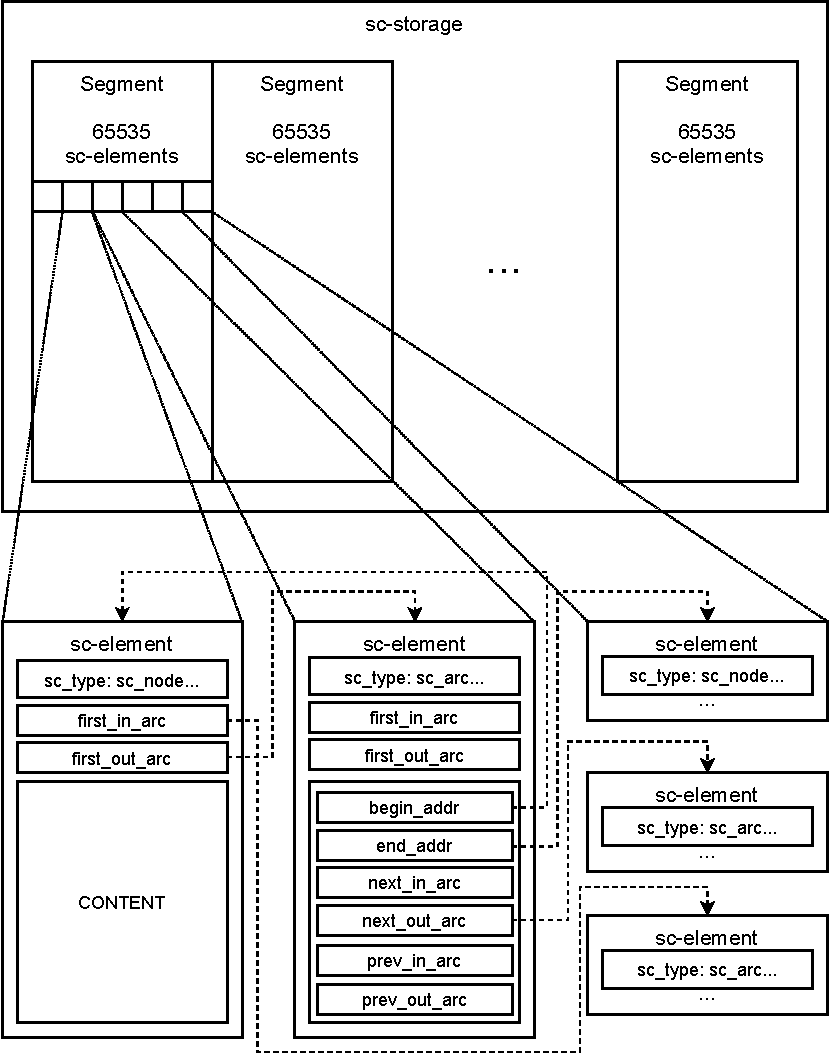
\includegraphics{figures/sd_interpreters/sc-storage.pdf}}}
\scnexplanation{В рамках данной программной реализации \textit{sc-хранилища} \scnbigspace \textit{sc-память} моделируется в виде набора \textit{сегментов}, каждый из которых состоит из фиксированного количества элементов sc-хранилища, каждый из которых соответствует конкретному sc-элементу. В настоящее время каждый сегмент состоит из $2^{16}-1=65535$ \textit{элементов sc-хранилища}.}
\scnrelfrom{класс объектов программной системы}{сегмент sc-хранилища}
\scnaddlevel{1}
	\scnnote{Максимально возможное число сегментов ограничивается настройками программной реализации sc-хранилища (в настоящее время по умолчанию установлено количество $2^{16}-1=65535$ сегментов). Таким образом, технически максимальное количество хранимых sc-элементов в текущей реализации составляет около $4.3 \times 10^{9}$ sc-элементов.}
	\scnnote{По умолчанию все сегменты физически располагаются в оперативной памяти, если объема памяти не хватает, то предусмотрен механизм выгрузки части сегментов на жесткий диск.}
	\scnrelfrom{класс объектов программной системы}{элемент sc-хранилища}
		\scnaddlevel{1}
			\scnexplanation{Каждый сегмент состоит из набора структур данных, описывающих конкретные \textit{sc-элементы} (элементов sc-хранилища). Независимо от типа описываемого sc-элемента каждый элемент sc-хранилища имеет фиксированный размер (в текущий момент -- 56 байт), что обеспечивает удобство их хранения. Таким образом, максимальный размер базы знаний в текущий момент в физическом выражении может достигнуть 223 Гб (без учета содержимого \textit{внутренних файлов ostis-системы}, хранимого на внешней файловой системе).}
		\scnaddlevel{-1}
\scnaddlevel{-1}

\scnheader{sc-адрес}
\scnidtf{адрес элемента sc-хранилища, соответствующего заданному sc-элементу, в рамках текущего состояния модели sc-памяти в составе программной реализации sc-хранилища}
\scnexplanation{Каждый элемент sc-хранилища в текущей реализации может быть однозначно задан его адресом (sc-адресом), состоящим из номера сегмента и номера sc-элемента в рамках сегмента. Таким образом, sc-адрес служит }
\scnnote{Sc-адрес никак не учитывается при обработке базы знаний на семантическом уровне и необходим только для обеспечения доступа к соответствующей структуре данных, хранящейся в линейной памяти на уровне реализации sc-хранилища.}
\scnnote{В общем случае sc-адрес элемента sc-хранилища, соответствующего заданному sc-элементу, может меняться, например, при пересборке базы знаний из исходных текстов и последующем перезапуске системы. При этом sc-адрес элемента sc-хранилища, соответствующего заданному sc-элементу, непосредственно в процессе работы системы в текущей реализации меняться не может.}
\scnnote{Для простоты будем говорить "sc-адрес sc-элемента", имея в виду \textit{sc-адрес} \scnbigspace \textit{элемента sc-хранилища}, однозначно соответствующего данному \textit{sc-элементу}.}
\scnrelfrom{обобщенная структура}{номер сегмента sc-хранилища;номер элемента sc-хранилища в рамках сегмента}

\scnheader{элемент sc-хранилища}
\scnidtf{ячейка sc-хранилища}
\scnidtf{элемент sc-хранилища, соответствующий sc-элементу}
\scnidtf{образ sc-элемента в рамках программной реализации sc-хранилища}
\scnidtf{структура данных, каждый экземпляр которой соответствует одному sc-элементу в рамках программной реализации sc-хранилища}
\scnexplanation{Каждый элемент sc-хранилища, соответствующий некоторому sc-элементу, описывается его синтаксическим типом (меткой), а также независимо от типа указывается sc-адрес первой входящей в данный sc-элемент sc-дуги и первой выходящей из данного sc-элемента sc-дуги (могут быть пустыми, если таких sc-дуг нет). 
	
Оставшиеся байты в зависимости от типа соответствующего sc-элемента (sc-узел или sc-дуга) могут использоваться либо для хранения содержимого внутреннего файла ostis-системы (может быть пустым, если sc-узел не является знаком файла), либо для хранения спецификации sc-дуги.}
\scnsubdividing{элемент sc-хранилища, соответствующий sc-узлу\\
	\scnaddlevel{1}
		\scnrelfromset{обобщенная структура}{метаинформация элемента sc-хранилища;sc-адрес первой sc-дуги, выходящей из данного sc-элемента;sc-адрес первой sc-дуги, входящей в данный sc-элемент;содержимое элемента sc-хранилища\\
		\scnaddlevel{1}
			\scnidtf{содержимое элемента sc-хранилища, соответствующего внутреннему файлу ostis-системы}
			\scnexplanation{
			Каждый sc-узел в текущей реализации может иметь содержимое (может стать \textit{внутренним файлом ostis-системы}).
			В случае, если размер содержимого внутреннего файла ostis-системы не превышает 48 байт (размер \textit{спецификации sc-дуги в рамках sc-хранилища}, например небольшой \textit{строковый идентификатор}), то это содержимое явно хранится в рамках элемента sc-хранилища в виде последовательности байт.
			В противном случае оно помещается в специальным образом организованную файловую память (за ее организацию отвечает отдельный модуль платформы, который в общем случае может быть устроен по-разному), а в рамках элемента sc-хранилища хранится уникальный адрес соответствующего файла, позволяющий быстро найти его на файловой системе.}
		\scnaddlevel{-1}}
		\scnaddlevel{1}
			\scnnote{\textit{sc-адрес первой sc-дуги, выходящей из данного sc-элемента}, \textit{sc-адрес первой sc-дуги, входящей в данный sc-элемент} и \textit{содержимое элемента sc-хранилища} в общем случае могут отсутствовать (быть нулевыми, "пустыми"), но размер элемента в байтах останется тем же.}
		\scnaddlevel{-1}
	\scnaddlevel{-1}
	;элемент sc-хранилища, соответствующий sc-дуге\\
	\scnaddlevel{1}
	\scnrelfromset{обобщенная структура}{метаинформация элемента sc-хранилища;sc-адрес первой sc-дуги, выходящей из данного sc-элемента;sc-адрес первой sc-дуги, входящей в данный sc-элемент;спецификации sc-дуги в рамках sc-хранилища\\
		\scnaddlevel{1}
			\scnrelfromset{обобщенная структура}{sc-адрес начального sc-элемента sc-дуги;sc-адрес конечного sc-элемента sc-дуги;sc-адрес следующей sc-дуги, выходящей из того же sc-элемента;sc-адрес следующей sc-дуги, входящей в тот же sc-элемент;sc-адрес предыдущей sc-дуги, выходящей из того же sc-элемента;sc-адрес предыдущей sc-дуги, входящей в тот же sc-элемент}
		\scnaddlevel{-1}}
	\scnnote{sc-ребра в текущий момент хранятся так же, как sc-дуги, то есть имеют начальный и конечный sc-элементы, отличие заключается только в \textit{метке синтаксического типа sc-элемента}. Это приводит к ряду неудобств при обработке, но sc-ребра используются в настоящее время достаточно редко.}
	\scnaddlevel{-1}}
\scnaddlevel{1}
	\scnnote{С точки зрения программной реализации структура данных для хранения sc-узла и sc-остается остается та же, но в ней меняется список полей (компонентов).\\
	Кроме того, как можно заметить каждый элемент sc-хранилища (в том числе, \textit{элемент sc-хранилища, соответствующий sc-дуге}) не хранит список sc-адресов связанных с ним sc-элементов, а хранит sc-адреса одной выходящей и одной входящей дуги, каждая из которых в свою очередь хранит sc-адреса следующей и предыдущей дуг в списке исходящих и входящих sc-дуг для соответствующих элементов.\\
	Все перечисленное позволяет:
	\begin{scnitemize}	
		\item сделать размер такой структуры фиксированным (в настоящее время 56 байт) и не зависящим от синтаксического типа хранимого sc-элемента;
		\item обеспечить возможность работы с sc-элементами без учета их синтаксического типа в случаях, когда это необходимо (например, при реализации поисковых запросов вида ``Какие sc-элементы являются элементами данного множества'', ``Какие sc-элементы непосредственно связаны с данным sc-элементом'' и т.д.);
	\end{scnitemize}}
\scnaddlevel{-1}

\scnheader{метаинформация элемента sc-хранилища}
\scnrelfromset{обобщенная структура}{метка синтаксического типа sc-элемента;метка уровня доступа sc-элемента}

\scnheader{метка синтаксического типа sc-элемента}
\scnsuperset{метка sc-узла}
\scnaddlevel{1}
	\scntext{числовое выражение в шестнадцатеричной системе}{0x1}
\scnaddlevel{-1}
\scnsuperset{метка внутреннего файла ostis-системы}
\scnaddlevel{1}
\scntext{числовое выражение в шестнадцатеричной системе}{0x2}
\scnaddlevel{-1}
\scnsuperset{метка sc-ребра общего вида}
\scnaddlevel{1}
\scntext{числовое выражение в шестнадцатеричной системе}{0x4}
\scnaddlevel{-1}
\scnsuperset{метка sc-дуги общего вида}
\scnaddlevel{1}
\scntext{числовое выражение в шестнадцатеричной системе}{0x8}
\scnaddlevel{-1}
\scnsuperset{метка sc-дуги принадлежности}
\scnaddlevel{1}
\scntext{числовое выражение в шестнадцатеричной системе}{0x10}
\scnaddlevel{-1}
\scnsuperset{метка sc-константы}
\scnaddlevel{1}
\scntext{числовое выражение в шестнадцатеричной системе}{0x20}
\scnaddlevel{-1}
\scnsuperset{метка sc-переменной}
\scnaddlevel{1}
\scntext{числовое выражение в шестнадцатеричной системе}{0x40}
\scnaddlevel{-1}
\scnsuperset{метка позитивной sc-дуги принадлежности}
\scnaddlevel{1}
\scntext{числовое выражение в шестнадцатеричной системе}{0x80}
\scnaddlevel{-1}
\scnsuperset{метка негативной sc-дуги принадлежности}
\scnaddlevel{1}
\scntext{числовое выражение в шестнадцатеричной системе}{0x100}
\scnaddlevel{-1}
\scnsuperset{метка нечеткой sc-дуги принадлежности}
\scnaddlevel{1}
\scntext{числовое выражение в шестнадцатеричной системе}{0x200}
\scnaddlevel{-1}
\scnsuperset{метка постоянной sc-дуги}
\scnaddlevel{1}
\scntext{числовое выражение в шестнадцатеричной системе}{0x400}
\scnaddlevel{-1}
\scnsuperset{метка временной sc-дуги}
\scnaddlevel{1}
\scntext{числовое выражение в шестнадцатеричной системе}{0x800}
\scnaddlevel{-1}
\scnsuperset{метка небинарной sc-связки}
\scnaddlevel{1}
\scntext{числовое выражение в шестнадцатеричной системе}{0x80}
\scnaddlevel{-1}
\scnsuperset{метка sc-структуры}
\scnaddlevel{1}
\scntext{числовое выражение в шестнадцатеричной системе}{0x100}
\scnaddlevel{-1}
\scnsuperset{метка ролевого отношения}
\scnaddlevel{1}
\scntext{числовое выражение в шестнадцатеричной системе}{0x200}
\scnaddlevel{-1}
\scnsuperset{метка неролевого отношения}
\scnaddlevel{1}
\scntext{числовое выражение в шестнадцатеричной системе}{0x400}
\scnaddlevel{-1}
\scnsuperset{метка sc-класса}
\scnaddlevel{1}
\scntext{числовое выражение в шестнадцатеричной системе}{0x800}
\scnaddlevel{-1}
\scnsuperset{метка абстрактной сущности}
\scnaddlevel{1}
\scntext{числовое выражение в шестнадцатеричной системе}{0x1000}
\scnaddlevel{-1}
\scnsuperset{метка материальной сущности}
\scnaddlevel{1}
\scntext{числовое выражение в шестнадцатеричной системе}{0x2000}
\scnaddlevel{-1}
\scnsuperset{метка константной позитивной постоянной sc-дуги принадлежности}
\scnaddlevel{1}
\scnreltoset{пересечение}{метка sc-дуги принадлежности;метка sc-константы;метка позитивной sc-дуги принадлежности;метка постоянной sc-дуги}
\scnnote{\textit{метки синтаксических типов sc-элементов} могут комбинироваться между собой для получения более частных классов меток. С точки зрения программной реализации такая комбинация выражается операцией побитового сложения значений соответствующих меток.}
\scnaddlevel{-1}
\scnsuperset{метка переменной позитивной постоянной sc-дуги принадлежности}
\scnaddlevel{1}
\scnreltoset{пересечение}{метка sc-дуги принадлежности;метка sc-переменной;метка позитивной sc-дуги принадлежности;метка постоянной sc-дуги}
\scnaddlevel{-1}
\scnnote{Числовые выражения некоторых классов меток могут совпадать. Это сделано для уменьшения размера элемента sc-хранилища за счет уменьшения максимального размера метки. Конфликт в данном случае не возникает, поскольку такие классы меток не могут комбинироваться, например \textit{метка ролевого отношения} и \textit{метка нечеткой sc-дуги принадлежности}.}
\scnnote{Важно отметить, что каждому из выделенных классов меток (кроме классов, получаемых путем комбинации других классов) однозначно соответствует порядковый номер бита в линейной памяти, что можно заметить, глядя на соответствующие числовые выражения классов меток. Это означает, что классы меток не включаются друг в друга, например, указание \textit{метки позитивной sc-дуги принадлежности} не означает автоматическое указание \textit{метки sc-дуги принадлежности}. Это позволяет сделать операции комбинирования и сравнения меток более эффективными.}

\scnheader{метка уровня доступа sc-элемента}
\scnrelfromset{обобщенная структура}{метка уровня доступа sc-элемента на чтение;метка уровня доступа sc-элемента на запись}
\scnexplanation{В текущей реализации sc-хранилища реализован механизм меток уровня доступа. Каждому элементу sc-хранилища соответствует \textit{метка уровня доступа sc-элемента на чтение} и \textit{метка уровня доступа sc-элемента на запись}, каждая из которых выражается числом от 0 до 255. 
	
В свою очередь, каждому процессу (чаще всего, соответствующему некоторому sc-агенту), который пытается получить доступ к данному элементу sc-хранилища (прочитать или изменить его) соответствует уровень доступа на чтение и запись, выраженный в том же числовом диапазоне. Указанный уровень доступа для процесса является частью \textit{контекста процесса}. Доступ на чтение или запись к элементу sc-хранилища не разрешается, если уровень доступа соответственно на чтение или запись у процесса ниже, чем у элемента sc-хранилища, к которому осуществляется доступ.

Таким образом нулевое значение \textit{метки уровня доступа sc-элемента на чтение} и \textit{метки уровня доступа sc-элемента на запись} означает, что любой процесс может получить неограниченный доступ к данному элементу sc=хранилища.}


\scnheader{Механизм итераторов в семантической памяти}
\scnheader{Механизм шаблонов в семантической памяти}
\scnheader{Механизм контекстов процессов в семантической памяти}
\scnheader{Механизм блокировок элементов семантической памяти}
\scnrelfrom{описание}{\nameref{sec:sd_agents}}
\scnheader{Механизм обработки событий в семантической памяти}

\scnheader{Реализация файловой памяти ostis-системы}
\scnauthorcomment{Пишет Денис}

\scnheader{Реализация базового набора платформенно-зависимых sc-агентов и их общих компонентов}
\scnidtf{sc-kpm}
\scnrelfromlist{компонент программной системы}{Реализация базового набора поисковых sc-агентов\\
	\scnaddlevel{1}
		\scnrelfromlist{используемый язык программирования}{C}
		\scnrelfromlist{компонент программной системы}{Реализация Абстрактного sc-агента поиска семантической окрестности заданной сущности;Реализация Абстрактного sc-агента поиска всех сущностей, частных по отношению к заданной;Реализация Абстрактного sc-агента поиска всех сущностей, общих по отношению к заданной;Реализация Абстрактного sc-агента поиска всех sc-идентификаторов, соответствующих заданной сущности;Реализация Абстрактного sc-агента поиска базовых sc-дуг, инцидентных заданному sc-элементу\\
			\scnaddlevel{1}
				\scnrelfromlist{компонент программной системы}{Реализация Абстрактного sc-агента поиска базовых sc-дуг, входящих в заданный sc-элемент;Реализация Абстрактного sc-агента поиска базовых sc-дуг, выходящих из заданного sc-элемента;Реализация Абстрактного sc-агента поиска базовых sc-дуг, входящих в заданный sc-элемент, с указанием множеств, которым принадлежат эти sc-дуги;Реализация Абстрактного sc-агента поиска базовых sc-дуг, выходящих из заданного sc-элемента, с указанием множеств, которым принадлежат эти sc-дуги}
			\scnaddlevel{-1}}
	\scnaddlevel{-1}
	;Реализация базового механизма сборки информационного мусора\\
	\scnaddlevel{1}
		\scnrelfromlist{используемый язык программирования}{C}	
		\scnnote{Текущая реализация механизма сборки информационного мусора, содержит один sc-агент, реагирующий на явное добавление какого-либо sc-элемента во множество ``информационный мусор'' и осуществляющий физическое удаление этого sc-элемента из sc-памяти}
	\scnaddlevel{-1}
	;Реализация базового набора интерфейсных sc-агентов\\
	\scnaddlevel{1}
	\scnrelfromlist{используемый язык программирования}{C++}	
	\scnrelfromlist{компонент программной системы}{Реализация Абстрактного sc-агента обработки команд пользовательского интерфейса;Реализация Абстрактного sc-агента трансляции из внутреннего представления знаний во промежуточный транспортный формат\\
	\scnaddlevel{1}
		\scnnote{В настоящее время используется подход, при котором независимо от формы внешнего представления информации, информация хранимая в sc-памяти вначале транслируется в промежуточный транспортный формат на базе JSON, который затем обрабатывается sc-агентами пользовательского интерфейса, входящими в состав \textit{Реализации интерпретатора sc-моделей пользовательских интерфейсов}}
	\scnaddlevel{1}
	}
	\scnaddlevel{-1}
}

\scnheader{SCTP}
\scnidtf{Semantic Code Transfer Protocol}
\scnrelboth{аналогия}{HTTP}
\scnexplanation{SCTP представляет собой \textit{бинарный протокол}, позволяющий осуществлять операции чтения (поиска) и редактирования конструкций, хранящихся в sc-памяти, а также отслеживать события, происходящие в sc-памяти.

Взаимодействие между клиентом и сервером на протоколе SCTP осуществляется путем обмена \textit{sctp-командами}, каждая из которых представляет собой набор байт, предназначенный для машинной обработки (но не восприятия человеком).
}

\scnheader{sctp-команда}
\scnrelfromset{обобщенная декомпозиция}{заголовок sctp-команды\\
	\scnaddlevel{1}
		\scnidtf{часть sctp-команды, в которой указан её тип и некоторая дополнительная информация о ней}
	\scnaddlevel{-1}
	;аргументы sctp-команды\\
	\scnaddlevel{1}
		\scnidtf{часть sctp-команды, которая содержит её аргументы и размер которой может быть разным в зависимости от типа команды.}
	\scnaddlevel{-1}}
\scnrelfromlist{включение;пример}{sctp-команда удаления sc-элемента с указанным sc-адресом;sctp-команда создания нового sc-узла указанного типа;sctp-команда получения начального и конечного элемента sc-дуги}
\scnnote{Выполнение каждой sctp-команды предполагает наличие sctp-результата, однозначно соответствующего данной команде.}

\scnheader{SCTP}
\scntext{программная документация}{http://ostis-dev.github.io/sc-machine/net/sctp/}
\scnrelfromlist{недостаток}{\scnfileitem{Команды протокола SCTP являются низкоуровневыми (ориентированы на работу с единичными sc-элементами или простейшими sc-конструкциями из 3 или 5 элементов). Это приводит к тому, что выполнение даже несложного преобразования в базе знаний или ассоциативный поиск по набору взаимосвязанных конструкций выражаются в виде достаточно большого набора sctp-команд. С учетом того, что для каждой команды существует sctp-результат, также пересылаемый по сети, это излишне нагружает сеть и сильно ухудшает производительность системы в целом. Кроме того, производительность системы начинает сильно зависеть от пропускной способности сети.};
\scnfileitem{Протокол SCTP не предназначен для восприятия человеком}}
\scnrelfromlist{достоинство}{\scnfileitem{Протокол SCTP является кросс-платформенным};\scnfileitem{Протокол SCTP может быть достаточно просто реализован практически на любом языке программирования}}
\scnrelfromlist{обобщенная реализация}{sctp-сервер\\
	\scnaddlevel{1}
		\scnexplanation{Sctp-сервер обрабатывает sctp-команды, приходящие от разных sctp-клиентов, и обеспечивает их интерпретацию в sc-памяти.}
	\scnaddlevel{-1}
	;sctp-клиент\\
	\scnaddlevel{1}
		\scnexplanation{Sctp-клиенты в общем случае могут быть реализованы на разных языках программирования и иметь разный программный интерфейс. По сути задачей sctp-клиента является преобразование высокоуровневых команд представленных в форме, удобной программисту, в одну или более низкоуровневых sctp-команд, отправка их на сервер, ожидание sctp-результата и его интерпретация.}
	\scnaddlevel{-1}}

\scnheader{Реализация подсистемы взаимодействия с внешней средой с использованием протокола SCTP}
\scnrelfromlist{компонент программной системы}{Реализация sctp-сервера;Реализация sctp-клиента\\
	\scnaddlevel{1}
	\scnnote{\textit{Реализация подсистемы взаимодействия с внешней средой с использованием протокола SCTP} включает в себя \textit{Реализацию sctp-клиента} на языке C++, в то же время есть другие реализации \textit{sctp-клиентов} в рамках того же программного варианта реализации платформы, например, в рамках \textit{Реализации интерпретатора sc-моделей пользовательских интерфейсов}.}
	\scnaddlevel{-1}}

\scnheader{Реализация подсистемы взаимодействия с внешней средой с использованием протоколов на основе формата JSON}
\scnexplanation{В связи с большим числом недостатков протокола SCTP было принято решение о разработке другого протокола на основе какого-либо общепринятого текстового транспортного формата. В качестве такого формата был выбран формат JSON.}
\scnrelto{реализация}{Протокол взаимодействия с sc-памятью на основе JSON}
\scnaddlevel{1}
\scnnote{Данный протокол пока не имеет собственного названия}
\scntext{программная документация}{http://ostis-dev.github.io/sc-machine/http/websocket/}
\scnexplanation{В рамках \textit{Протокола взаимодействия с sc-памятью на основе JSON} каждая команда представляет собой json-объект, в котором указываются идентификатор команда, тип команды и ее аргументы. В свою очередь ответ на команду также представляет собой json-объект, в котором указываются идентификатор команды, ее статус (выполнена успешно/безуспешно) и результаты. Структура аргументов и результатов команды определяется типом команды.}
\scnrelfromlist{достоинство}{\scnfileitem{JSON является общепринятым открытым форматом, для работы с которым существует большое количество библиотек для популярных языков программирования. Это, в свою очередь, упрощает реализацию клиента и сервера для протокола, построенного на базе JSON.};
\scnfileitem{Реализация протокола на базе JSON не накладывает принципиальных ограничений на объем (длину) каждой команды, в отличие от бинарного протокола. Таким образом, появляется возможность использования неатомарных команд, позволяющих, например, за один акт пересылки такой команды по сети создать сразу несколько sc-элементов. Важными примерами таких команд являются  \textit{Команда генерации по произвольному образцу} и \textit{Команда поиска по произвольному образцу}.}}
\scnaddlevel{-1}

\scnheader{Реализация вспомогательных инструментальных средств в рамках реализации sc-памяти}
\scnrelfrom{компонент программной системы}{Реализация сборщика базы знаний из исходных текстов, записанных в SCs-коде}
\scnaddlevel{1}
\scnidtf{sc-builder}
\scnrelfrom{используемый язык}{SCs-код}
\scnexplanation{Сборщик базы знаний из исходных текстов позволяет осуществить сборку базы знаний из набора исходных текстов, записанных в SCs-коде с ограничениями (см. \textit{Раздел **про исходные тексты**}) в бинарный формат, воспринимаемый \textit{Реализацией sc-памяти}. При этом возможна как сборка "с нуля"{} (с уничтожением ранее созданного слепка памяти), так и аддитивная сборка, когда информация, содержащаяся в заданном множестве файлов, добавляется к уже имеющемуся слепку состояния памяти.

В текущей реализации сборщик осуществляет "склеивание"{} ("слияние"{}) sc-элементов, имеющих на уровне исходных текстов одинаковые \textit{системные sc-идентификаторы}.}
\scnaddlevel{-1}

\scnheader{Реализация интерпретатора sc-моделей пользовательских интерфейсов}
\scnidtf{sc-web}
\scnrelfromlist{используемый язык программирования}{JavaScript;TypeScript;Python}
\scnrelfrom{иллюстрация}{\scnfileimage{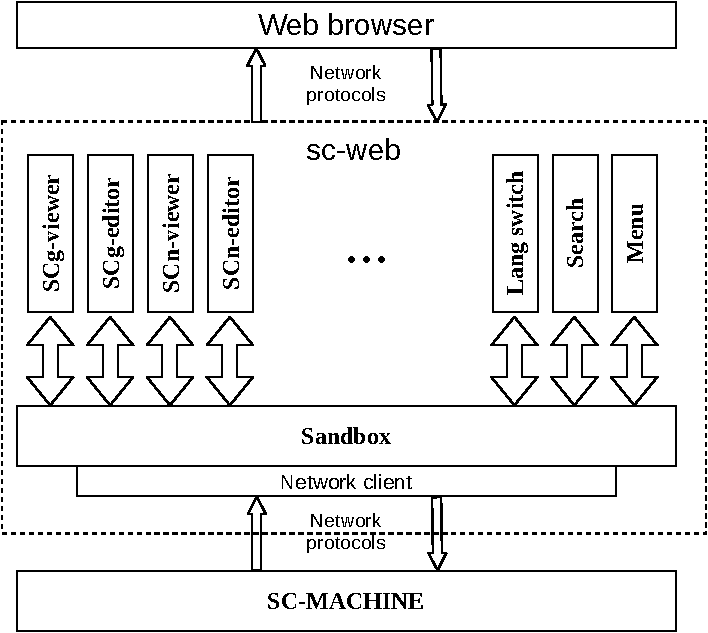
\includegraphics{figures/sd_interpreters/sc-web-new-arch.pdf}}}
\scnaddlevel{1}
	\scnexplanation{На данной иллюстрации показан планируемый вариант архитектуры \textit{Реализация интерпретатора sc-моделей пользовательских интерфейсов}, важным принципом которой является простота и однотипность подключения любых компонентов пользовательского интерфейса (редакторов, визуализаторов, переключателей, команд меню и т.д.). Для этого реализуется программная прослойка Sandbox, в рамках которой реализуются низкоуровневые операции взаимодействия с серверной частью и которая обеспечивает более удобный программный интерфейс для разработчиков компонентов.}
\scnaddlevel{-1}
\scnrelfromset{недостатки текущей реализации}{\scnfileitem{Отсутствие единого унифицированного механизма клиент-серверного взаимодействия. Часть компонентов (визуализатор sc-текстов в SCn-коде, команды меню и др.) работают по протоколу HTTP, часть по протоколу SCTP, это приводит к значительным трудностям при развитии платформы. 
Протокол HTTP предполагает четкое разделение активного клиента и пассивного сервера, который отвечает на запросы клиентов. Таким образом, сервер (в данном случае -- sc-память) практически не имеет возможности по своей инициативе отправить сообщение клиенту, что повышает безопасность системы, но значительно снижает ее интерактивность. Кроме того, такой вариант реализации затрудняет реализацию принятого в Технологии OSTIS многоагентного подхода, в частности, затрудняет реализацию sc-агентов на стороне клиента. Указанные проблемы могут быть решены путем постоянного мониторинга определенных событий со стороны клиента, однако такой вариант неэффективен.
Кроме того, часть интерфейса работает напрямую с sc-памятью (по протоколу SCTP), а часть -- через прослойку на базе библиотеки tornado для языка программирования Python, что приводит к дополнительным зависимостям от сторонних библиотек.};
\scnfileitem{Часть компонентов (например, поле поиска по идентификатору) реализована сторонними средствами и практически никак не связана с sc-памятью. Это затрудняет развитие платформы.};
\scnfileitem{Текущая \textit{Реализация интерпретатора sc-моделей пользовательских интерфейсов} ориентирована только на ведение диалога с пользователем (в стиле вопрос пользователя -- ответ системы). Не поддерживаются такие очевидно необходимые ситуации, как выполнение команды, не предполагающей ответа\char59~возникновение ошибки или отсутствие ответа\char59~необходимость задания вопроса системой пользователю и т.д.};
\scnfileitem{Ограничена возможность взаимодействия пользователя с системой без использования специальных элементов управления. Например, можно задать вопрос системе, нарисовав его в SCg-коде, но ответ пользователь не увидит, хотя в памяти он будет сформирован соответствующим агентом.;
Большая часть технологий, использованных при реализации платформы, к настоящему моменту устарела, что затрудняет развитие платформы.};
\scnfileitem{Идея платформенной независимости пользовательского интерфейса (построения sc-модели пользовательского интерфейса) реализована не в полной мере. Полностью описать sc-модель пользовательского интерфейса (включая точное размещение, размеры, дизайн компонентов, их поведение и др.) в настоящее время скорее всего окажется затруднительно из-за ограничений производительности, однако вполне возможно реализовать возможность задания вопросов ко всем компонентам интерфейса, изменить их расположение и т.д., однако эти возможности нельзя реализовать в текущей версии реализации платформы.};
\scnfileitem{Интерфейсная часть работает медленно из-за недостатков  протокола SCTP и некоторых недостатков реализации серверной части на языке Python.;
Не реализован механизм наследования при добавлении новых внешних языков. Например, добавление нового языка даже очень близкого к SCg-коду требует физического копирования кода компонента и внесение соответствующих изменений, при этом получаются два никак не связанных между собой компонента, которые начинают развиваться независимо друг от друга.};
\scnfileitem{Слабый уровень задокументированности текущей \textit{Реализации интерпретатора sc-моделей пользовательских интерфейсов}.}}
\scnrelfromset{требования к будущей реализации}{\scnfileitem{Унифицировать принципы взаимодействия всех компонентов интерфейса с \textit{Реализацией sc-памяти}, независимо от того, к какому типу относится компонент. Например, список команд меню должен формироваться через тот же механизм, что и ответ на запрос пользователя, и команда редактирования, сформированная пользователем, и команда добавления нового фрагмента в базу знаний и т.д.};
\scnfileitem{Унифицировать принципы взаимодействия пользователей с системой независимо от способа взаимодействия и внешнего языка. Например, должна быть возможность задания вопросов и выполнения других команд прямо через SCg/SCn интерфейс. При этом необходимо учитывать принципы редактирования базы знаний, чтобы пользователя не мог под видом задания вопроса внести новую информацию в согласованную часть базы знаний.};
\scnfileitem{Унифицировать принципы обработки событий, происходящих при взаимодействии пользователя с компонентами интерфейса -- поведение кнопок и других интерактивных компонентов должно задаваться не статически сторонними средствами, а реализовываться в виде агента, который, тем не менее, может быть реализован произвольным образом (не обязательно на платформенно-независимом уровне). Любое действие, совершаемое пользователем, на логическом уровне должно трактоваться и обрабатываться как инициирование агента.};
\scnfileitem{Обеспечить возможность выполнять команды (в частности, задавать вопросы) с произвольным количеством аргументов, в том числе -- без аргументов.};
\scnfileitem{Обеспечить возможность отображения ответа на вопрос по частям, если ответ очень большой и для отображения требуется много времени.};
\scnfileitem{Каждый отображаемый компонент интерфейса должен трактоваться как изображение некоторого sc-узла, описанного в базе знаний. Таким образом, пользователь должен иметь возможность задания произвольных вопросов к любым компонентам интерфейса.};
\scnfileitem{Максимально упростить и задокументировать механизм добавления новых компонентов.};
\scnfileitem{Обеспечить возможность добавления новых компонентов на основе имеющихся без создания независимых копий. Например, должна быть возможность создать компонент для языка, расширяющего язык SCg новыми примитивами, переопределять принципы размещения sc-текстов и т.д.};
\scnfileitem{Свести к минимуму зависимость от сторонних библиотек.};
\scnfileitem{Свести к минимуму использование протокола HTTP (начальная загрузка общей структуры интерфейса), обеспечить возможность равноправного двустороннего взаимодействия серверной и клиентской части.};
\scnfileitem{Полностью отказаться от протокола SCTP, перейти на протокол на базе JSON, задокументировать его.}}
\scnaddlevel{1}
	\scnnote{Очевидно, что реализация большинства из приведенных требований связана не только с собственно вариантом реализации платформы, но и требует развития теории логико-семантических моделей пользовательских интерфейсов и уточнения в рамках нее общих принципов организации пользовательских интерфейсов ostis-систем. Однако, принципиальная возможность реализации таких моделей должна быть учтена в рамках реализации платформы.}
\scnaddlevel{-1}

\scnheader{Реализация scp-интерпретатора}
\scnrelfromlist{используемый язык программирования}{C++}
\scnrelfromlist{компонент программной системы}{Реализация Абстрактного sc-агента создания scp-процессов;Реализация Абстрактного sc-агента интерпретации scp-операторов\\
	\scnaddlevel{1}
	\scnrelfromlist{компонент программной системы}{Реализация Абстрактного sc-агента интерпретации scp-операторов генерации конструкций;Реализация Абстрактного sc-агента интерпретации scp-операторов ассоциативного поиска конструкций;Реализация Абстрактного sc-агента интерпретации scp-операторов удаления конструкций;Реализация Абстрактного sc-агента интерпретации scp-операторов проверки условий		;Реализация Абстрактного sc-агента интерпретации scp-операторов управления значениями операндов;Реализация Абстрактного sc-агента интерпретации scp-операторов управления scp-процессами;Реализация Абстрактного sc-агента интерпретации scp-операторов управления событиями;Реализация Абстрактного sc-агента интерпретации scp-операторов обработки содержимых числовых файлов;Реализация Абстрактного sc-агента интерпретации scp-операторов обработки содержимых строковых файлов}
	\scnaddlevel{-1}
	;Реализация Абстрактного sc-агента синхронизации процесса интерпретации scp-программ;Реализация Абстрактного sc-агента уничтожения scp-процессов;Реализация Абстрактного sc-агента синхронизации событий в sc-памяти и ее реализации}
\scnnote{Текущая \textit{Реализация scp-интерпретатора} не включает в себя специализированных средств для работы с блокировками, поскольку механизм блокировок элементов sc-памяти реализован на более низком уровне в рамках \textit{Реализация sc-хранилища и механизма доступа к нему}}

\scnendstruct

\end{SCn}

\scsection{\textbf{Предметная область и онтология семантических ассоциативных компьютеров для ostis-систем}}
\label{sd_sem_comp}
\begin{SCn}

\scnsectionheader{Предметная область и онтология семантических ассоциативных компьютеров для ostis-систем}

\scnstartsubstruct

\scnheader{Предметная область и онтология семантических ассоциативных компьютеров для ostis-систем}
\scnsdmainclasssingle{***}
\scnsdclass{***}
\scnsdrelation{***}

\scnheader{семантический ассоциативный компьютер}
\scnidtf{аппаратно реализованный интерпретатор семантических моделей (sc-моделей) компьютерных систем}
\scnidtf{семантический ассоциативный компьютер, управляемый знаниями}
\scnidtf{компьютер с нелинейной структурно перестраиваемой (графодинамической) ассоциативной памятью, переработка информации в которой сводится не к изменению состояния элементов памяти, а к изменению конфигурации связей между ними}
\scnidtf{sc-компьютер}
\scnidtf{scp-компьютер}
\scnidtf{компьютер, управляемый знаниями, представленными в SC-коде}
\scnidtf{компьютер, ориентированный на обработку текстов SC-кода}

\filemodetrue
\scnrelfromlist{принцип}{
нелинейная память — каждый элементарный фрагмент хранимого в памяти текста может быть инцидентен неограниченному числу других элементарных фрагментов этого текста;
структурно перестраиваемая (реконфигурируемая) память — процесс отработки хранимой в памяти информации сводится не только к изменению состояния элементов, но и к реконфигурации связей между ними;
в качестве внутреннего способа кодирования знаний, хранимых в памяти семантического ассоциативного компьютера, используется универсальный (!) способ нелинейного (графоподобного) смыслового представления знаний, названный нами SC-кодом (семантическим, смысловым компьютерным кодом);
обработка информации осуществляется коллективом агентов, работающих над общей памятью. Каждый из них реагирует на соответствующую ему ситуацию или событие в памяти (компьютер, управляемый хранимыми знаниями);
есть программно реализуемые агенты, поведение которых описывается хранимыми в памяти агентно-ориентированными программами, которые интерпретируются соответствующими коллективами агентов;
есть базовые агенты, которые не могут быть реализованы программно (в частности, это агенты интерпретации агентных программ, базовые рецепторные агенты-датчики, базовые эффекторные агенты);
все агенты работают над общей памятью одновременно. Более того, если для какого-либо агента в некоторый момент времени в различных частях памяти возникает сразу несколько условий его применения, разные акты указанного агента в разных частях памяти могут выполняться одновременно (акт агента — это неделимый, целостный процесс деятельности агента);
для того, чтобы акты агентов, параллельно выполняемые в общей памяти не "мешали"\ друг другу, для каждого акта в памяти фиксируется и постоянно актуализируется его текущее состояние. То есть каждый акт сообщает всем остальным о своих намерениях и пожеланиях, которым остальные агенты не должны препятствовать (например, это различного рода блокировки используемых элементов семантической памяти);
кроме того, агенты (точнее, выполняемые ими акты) должны соблюдать "этику"\,, стараясь не в ущерб себе создавать максимально благоприятные условия для других агентов (актов), например, не жадничать, быстрее возвращать, не захватывать (не блокировать) лишние элементы памяти, как можно скорее освобождать (деблокировать) заблокированные элементы памяти;
процессор и память семантического ассоциативного компьютера глубоко интегрированы и составляют единую процессоро-память. Процессор семантического ассоциативного компьютера равномерно "распределен"\ по его памяти так, что процессорные элементы одновременно являются и элементами памяти компьютера. Обработка информации в семантическом ассоциативном компьютере сводится к реконфигурации каналов связи между процессорными элементами,  следовательно память такого компьютера есть не что иное, как \uline{коммутатор} (!) указанных каналов связи. Таким образом, текущее состояние конфигурации этих каналов связи и есть текущее состояние обрабатываемой информации}
\filemodefalse

\scnendstruct

\end{SCn}

\newpage
\scchapter{Предметная область и онтология Экосистемы OSTIS}
\begin{SCn}

\scnsectionheader{\currentname}

\scnstartsubstruct

\scnrelfromlist{дочерний раздел}{\nameref{sd_learning};\nameref{sd_assistants};\nameref{sd_portals};\nameref{sd_ecosys_enterprise}}

\scnheader{Предметная область Экосистемы OSTIS}
\scniselement{предметная область}

\scnsdmainclasssingle{Экосистема OSTIS}
\scnsdclass{ostis-система;самостоятельная ostis-система;поддержка совместимости между компьютерными системами и их пользователями в Экосистеме OSTIS}

\scnheader{Проект OSTIS}
\scnidtf{Проект, направленный на создание \textit{Технологии OSTIS} и, в частности, на разработку  \textit{Стандарта OSTIS}}
\scnrelfromlist{продукт}{
	Технология OSTIS;
	Метасистема OSTIS\\
	\scnaddlevel{1}
	\scnidtf{Метасистема IMS.ostis}
	\scnaddlevel{-1};
	Стандарт OSTIS;
	Экосистема OSTIS}
\scnrelfromlist{подпроект}{Проект разработки Технологии OSTIS;
	Проект разработки Метасистемы OSTIS; Проект разработки Стандарта OSTIS;Проект разработки Экосистемы OSTIS}
\scnrelfromlist{библиографический источник}{\scncite{DeNicola2021};\scncite{Alrehaili2021};\scncite{Alrehaili2017};\scncite{Shahzad2021}}

\scnheader{Экосистема OSTIS}
\scnidtf{Социотехническая экосистема, представляющая собой коллектив взаимодействующих семантических компьютерных систем и осуществляющая перманентную поддержку эволюции и семантической совместимости всех входящих в нее систем, на протяжении всего их жизненного цикла}
\scnidtf{Неограниченно расширяемый коллектив постоянно эволюционируемых семантических компьютерных систем, которые взаимодействуют между собой и с пользователями для корпоративного решения сложных задач и для постоянной поддержки высокого уровня совместимости и взаимопонимания во взаимодействии как между собой, так и с пользователями}

\scnexplanation{Поскольку \textit{Технология OSTIS} ориентирована на разработку \textit{семантических компьютерных систем}, обладающих высоким уровнем \textit{обучаемости} и, в частности, высоким уровнем семантической \textit{совместимости}, и поскольку обучаемость и совместимость есть только \uline{способность} к обучению (т.е. к высоким темпам расширения и совершенствования своих знаний и навыков), а также \uline{способность} к обеспечению высокого уровня взаимопонимания (согласованности), необходима некая среда, социотехническая инфраструктура, в рамках которой были бы созданы максимально комфортные условия для реализации указанных выше способностей. Такая среда названа нами \textit{\textbf{Экосистемой OSTIS}}, которая представляет собой коллектив взаимодействующих (через сеть Интернет):

\begin{scnitemize}
\item самих \textit{ostis-систем};
\item пользователей указанных \textit{ostis-систем} (как конечных пользователей, так и разработчиков);
\item некоторых компьютерных систем, не являющихся \textit{ostis-системами}, но рассматриваемых ими в качестве дополнительных информационных ресурсов или сервисов.
\end{scnitemize}
}
\scntext{основная задача}{Обеспечить постоянную поддержку совместимости компьютерных систем, входящих в \textit{Экосистему OSTIS} как на этапе их разработки, так и в ходе их эксплуатации. Проблема здесь заключается в том, что в ходе эксплуатации систем, входящих в \textit{Экосистему OSTIS}, они могут изменяться из-за чего совместимость может нарушаться.

Задачами \textit{Экосистемы OSTIS} являются:
\begin{scnitemize}
\item оперативное внедрение всех согласованных изменений стандарта \textit{ostis-систем} (в том числе, и изменений систем используемых понятий и соответствующих им терминов);
\item перманентная поддержка высокого уровня взаимопонимания всех систем, входящих в \textit{Экосистему OSTIS}, и всех их пользователей; 
\item корпоративное решение различных сложных задач, требующих координации деятельности нескольких (чаще всего, априори неизвестных) \textit{ostis-систем}, а также, возможно, некоторых пользователей.
\end{scnitemize}
}
\scnnote{\textit{Экосистема OSTIS} -- это переход от самостоятельных (автономных, отдельных, целостных) \textit{ostis-систем} к коллективам самостоятельных \textit{ostis-систем}, т.е. к распределенным \textit{ostis-системам}}

\scnheader{ostis-система}
\scnsubdividing{самостоятельная ostis-система\\
	\scnaddlevel{1}
	\scnidtf{целостная \textit{ostis-система}, которая должна самостоятельно решать соответствующее множество задач и, в частности, взаимодействовать с внешней средой (как вербально -- с пользователями и другими компьютерными системами, так и невербально)}
	\scnaddlevel{-1};
	встроенная ostis-система\\
	\scnaddlevel{1}
		\scnidtf{интеллектуальная компьютерная подсистема, разработанная по \textit{Технологии OSTIS} и реализующая часть функционала \textit{ostis-системы} более высокого уровня иерархии}
		\scnidtf{\textit{ostis-система}, интегрированная в состав \textit{самостоятельной ostis-системы}}
		\scnsubdividing{атомарная встроенная ostis-система\\
		\scnaddlevel{1}
			\scnidtf{\textit{встроенная ostis-система}, не включающая в себя какие-либо другие \textit{встроенные ostis-системы}}
		\scnaddlevel{-1};
		неатомарная встроенная ostis-система\\
		\scnaddlevel{1}
			\scnsuperset{интерфейс ostis-системы}
		\scnaddlevel{-1}
		}
	\scnaddlevel{-1};
	коллектив ostis-систем\\
	\scnaddlevel{1}
		\scnidtf{группа общающихся ostis-систем, в состав которой могут входить не только самостоятельные ostis-системы, но и коллективы ostis-систем}
		\scnidtf{распределенная ostis-система}
	\scnaddlevel{-1}
}

\scnheader{самостоятельная ostis-система}
\scnexplanation{Подчеркнем, что к \textit{\textbf{самостоятельным ostis-системам}}, входящим в состав \textit{Экосистемы OSTIS}, предъявляются особые требования:
\begin{scnitemize}
    \item они должны обладать всеми необходимыми знаниями и навыками для обмена сообщениями и целенаправленной организации взаимодействия с другими \textit{ostis-системам}и, входящими в \textit{Экосистему OSTIS};
    \item в условиях постоянного изменения и эволюции \textit{ostis-систем}, входящих в \textit{Экосистему OSTIS}, каждая из них должна \uline{сама следить за состоянием своей совместимости} (согласованности) со всеми остальными \textit{ostis-системами},  т.е. должна самостоятельно поддерживать эту совместимость, согласовывая с другими ostis-системами все требующие согласования изменения, происходящие у себя и в других системах.
    \item каждая система, входящая в состав \textit{Экосистемы OSTIS}, должна:
    \begin{scnitemizeii}
        \item интенсивно, активно и целенаправленно обучаться ( как с помощью  учителей-разработчиков, так и самостоятельно);
        \item сообщать всем другим системам о предлагаемых или окончательно утвержденных изменениях в \textit{онтологиях} и, в частности, в наборе используемых \textit{понятий};
        \item принимать от других \textit{ostis-систем} предложения об изменениях в \textit{онтологиях} ( в том числе в наборе используемых понятий) для согласования или утверждения этих предложений;
        \item реализовывать утвержденные изменения в \textit{онтологиях}, хранимых в ее базе знаний;
        \item способствовать поддержанию высокого уровня семантической совместимости не только с другими \textit{ostis-системами}, входящими в \textit{Экосистему OSTIS}, но и со своими \textit{пользователями} ( т.е. обучать их, информировать их об изменениях в онтологиях).
    \end{scnitemizeii}
\end{scnitemize}}

\scnheader{Экосистема OSTIS}
\scnexplanation{\textit{Экосистема OSTIS} является формой реализации, совершенствования и применения \textit{Технологии OSTIS} и, следовательно, является формой создания, развития, самоорганизации рынка семантически совместимых компьютерных систем  и включает в себя все необходимые для этого ресурсы --  информационные, технологические, кадровые, организационные, инфраструктурные. 

\textit{Экосистеме OSTIS} ставится в соответствие ее \textit{\textbf{объединенная база знаний}}, которая представляет собой \textbf{виртуальное объединение} \textit{баз знаний} всех \textit{ostis-систем}, входящих в состав \textit{Экосистемы OSTIS}. Качество этой \textit{базы знаний} (полнота, непротиворечивость, чистота) является постоянной заботой всех самостоятельных \textit{ostis-систем}, входящих в состав \textit{Экосистемы OSTIS}. Соответственно этому каждой указанной \textit{ostis-системе} ставится в соответствие своя \textit{база знаний} и своя иерархическая система \textit{sc-агентов}.

По назначению \textit{ostis-системы}, входящие в \textit{Экосистему OSTIS}, могут быть:
\begin{scnitemize}
    \item ассистентами конкретных пользователей или конкретных пользовательских коллективов;
    \item типовыми встраиваемыми подсистемами \textit{ostis-систем};
    \item системами информационной и инструментальной поддержки проектирования различных компонентов и различных классов \textit{ostis-систем};
    \item системами информационной и инструментальной поддержки проектирования или производства различных классов технических и других искусственно создаваемых систем;
    \item порталами знаний по самым различным научным дисциплинам; 
    \item системами автоматизации управления различными сложными объектами (производственными предприятиями, учебными заведениями, кафедрами вузов, конкретными обучаемыми);
    \item интеллектуальными справочными и help-системами;
    \item интеллектуальными обучающими системами, семантическими электронными учебными пособиями;
    \item интеллектуальными робототехническими системами.
\end{scnitemize}
}

\scnresetlevel

\scnheader{поддержка совместимости между компьютерными системами и их пользователями в Экосистеме OSTIS}
\scnexplanation{Есть три аспекта поддержки совместимости и взаимопонимания в \textit{Экосистеме OSTIS}

\begin{scnitemize}
\item поддержка совместимости между самими \textit{ostis-системами}, входящими в \textit{Экосистему OSTIS} в процессе их эволюции;
\item поддержка совместимости между каждой ostis-системой и текущим состоянием Технологии OSTIS в процессе эволюции этой технологии;
\item поддержка совместимости и взаимопонимания между \textit{ostis-системами}, входящими в \textit{Экосистему OSTIS}, и их пользователями при активном стимулировании со стороны \textit{Экосистемы OSTIS} того, чтобы каждый пользователь \textit{Экосистемы OSTIS} был одновременно не только активным ее конечным пользователем, но и активным ее разработчиком.
\end{scnitemize}

Таким образом, для обеспечения высокой эффективности эксплуатации и высоких темпов эволюции  \textit{Экосистемы OSTIS}, необходимо постоянно повышать уровень информационной совместимости (уровень взаимопонимания) не только между компьютерными системами, входящими в состав \textit{Экосистемы OSTIS}, но также между этими системами и их пользователями. Одним из направлений обеспечения такой совместимости является стремление к тому, чтобы \textit{база знаний} (картина мира) каждого пользователя стала частью (фрагментом) \textbf{\textit{Объединенной базы знаний Экосистемы OSTIS}}.  Это значит, что каждый пользователь должен знать, как устроена структура каждой научно-технической дисциплины (объекты исследования, предметы исследования, определения, закономерности и т.д.), как могут быть связаны между собой различные дисциплины.

Формирование таких навыков системного построения картины Мира необходимо начинать со средней школы. Для этой цели необходимо создать комплекс совместимых интеллектуальных обучающих систем по всем дисциплинам среднего образования с четко описанными междисциплинарными связями (\scncite{Bashmakov}, \scncite{Taranchuk2015}). Благодаря этому можно предотвратить формирование у пользователей "мозаичной"{} картины Мира как множества слабо связанных между собой дисциплин. А это, в свою очередь, означает существенное повышение качества образования, которое абсолютно необходимо для качественной эксплуатации компьютерных систем следующего поколения -- \textit{семантических компьютерных систем}.

Пользователи и, первую очередь, разработчики \textit{Экосистемы OSTIS}  должны иметь высокий уровень:
\begin{scnitemize}
\item математической культуры (культуры формализации) при построении формальной модели среды, в которой функционирует интеллектуальная система, формальных моделей решаемых ею задач и формальных моделей различных используемых ею способов решения задач;
\item системной культуры, позволяющей адекватно оценивать качество разрабатываемых систем с точки зрения общей теории систем и, в частности, оценивать общий уровень автоматизации, реализуемый с помощью этих систем. Системная культура предполагает стремление и умение избегать эклектики, стремление и умение обеспечить качественную стратифицированность, гибкость, рефлексивность, а также качественное сопровождение, высокий уровень обучаемости и комфортный пользовательский интерфейс разрабатываемых систем;
\item технологической культуры, обеспечивающей совместимость разрабатываемых систем и их компонентов, а также постоянное расширение библиотеки многократно используемых компонентов создаваемых систем и предполагающей высокий уровень проектной дисциплины;
\item умения работать в команде разработчиков наукоемких систем, что предполагает высокий уровень умения работать на междисциплинарных стыках, высокий уровень коммуникабельности и \uline{договороспособности}, т.е. способности не столько отстаивать свою точку зрения, сколько согласовывать ее  с точками зрения других разработчиков в интересах развития \textit{Экосистемы OSTIS};
\item активности и ответственности за общий результат -- высокие темпы эволюции \textit{Экосистемы OSTIS} в целом.
\end{scnitemize}

Таким образом высокие темпы эволюции \textit{Экосистемы OSTIS} обеспечиваются не только профессиональной квалификацией пользователей (знаниями о \textit{Технологии OSTIS}, о текущем состоянии и проблемах \textit{Экосистемы OSTIS} и навыками использования \textit{Технологии OSTIS} и интеллектуальных систем, входящих в \textit{Экосистему OSTIS}), но и соответствующими человеческими качествами. Очевидно, что современный уровень \uline{договороспособности, активности и ответственности} не может быть основой для эволюции таких систем, как \textit{Экосистема OSTIS}.

Поддержка совместимости \textit{Экосистемы OSTIS} с ее пользователями осуществляется следующим образом:


\begin{scnitemize}
\item в каждую \textit{ostis-систему} включаются встроенные ostis-системы, ориентированные
  
  \begin{scnitemizeii}
        \item на перманентный мониторинг деятельности конечных пользователей и разработчиков этой \textit{\mbox{ostis-системы}},
        \item на анализ качества и, в первую очередь, корректности этой деятельности,
        \item на перманентное ненавязчивое персонифицированное обучение, направленное на повышение качества деятельности пользователей, т.е. на повышение их квалификации;
        
  \end{scnitemizeii}
        
\item в состав \textit{Экосистемы OSTIS} включаются \textit{ostis-системы}, специально предназначенные для обучения пользователей \textit{Экосистемы OSTIS} базовым общепризнанным знаниям и навыкам решения соответствующих классов задач. Сюда входят и знания, соответствующие уровню среднего образования, и знания соответствующие базовым дисциплинам высшего образования в области информатики (и, в том числе, в области искусственного интеллекта), и базовые знания по \textit{Технологии OSTIS} и об \textit{Экосистеме OSTIS}.

\end{scnitemize}}

\scnheader{Экосистема OSTIS}
\scntext{обоснование}{Проблема создания рынка совместимых компьютерных систем --  \textbf{вызов современной науке и технике}.  От ученых, работающих в области искусственного интеллекта требуется умение коллективно работать над решением междисциплинарных проблем и доводить эти решения до общей интегрированной теории интеллектуальных систем, предполагающей интеграцию всех направлений искусственного интеллекта, и до технологий, доступных широкому кругу инженеров. От инженеров интеллектуальных систем требуется активное участие в развитии соответствующих технологий и существенное повышение уровня математической, системный, технологической и организационно-психологической культуры.

Но главной задачей здесь является снижение барьера между научными исследованиями в области искусственного интеллекта и инженерией в области разработки интеллектуальных систем. Для этого наука должна стать конструктивной и ориентированной на интеграцию своих результатов в форме комплексной технологии разработки интеллектуальных систем, а инженерия, осознав наукоемкость своей деятельности, должна активно участвовать в разработке технологий.

Особый акцент в \textit{Экосистеме OSTIS}  делается на постоянный процесс согласования \textit{онтологий} (и, в первую очередь, на согласование семейства всех используемых понятий и терминов, соответствующих этим понятиям) между \uline{всеми} (!) активными субъектами \textit{Экосистемы OSTIS} -- между всеми \textit{ostis-системами} и всеми пользователями.

При наличии \textit{ostis-систем}, являющихся персональными ассистентами пользователей во взаимодействии с \textit{Экосистемой OSTIS}, вся эта Экосистема будет восприниматься пользователями как единая интеллектуальная система, объединяющая все имеющиеся в \textit{Экосистеме OSTIS} информационные ресурсы и сервисы.

Принципы организации \textit{Экосистемы OSTIS} создают все необходимые условия для привлечения к разработке и совершенствованию \textit{Технологии OSTIS} научные, организационные и финансовые ресурсы, которые будут направлены на развитие методов и средств искусственного интеллекта и на формирование рынка семантически совместимых интеллектуальных систем.}

\bigskip
\scnendstruct \scnendcurrentsectioncomment

\end{SCn}


\scsection{Предметная область и онтология методов и средств реализации информационно-справочных возможностей для каждой ostis-системы, входящей в состав Экосистемы OSTIS}

\scsection{Предметная область и онтология методов и средств реализации целенаправленного и персонифицированного процесса обучения пользователей для каждой ostis-системы, входящей в состав Экосистемы OSTIS}

\scsection{Предметная область и онтология ostis-систем, являющихся персональными ассистентами пользователей в рамках Экосистемы OSTIS}

\scsection{Предметная область и онтология семантически совместимых интеллектуальных порталов научно-технических знаний}
\label{sec:sd_portals}
\begin{SCn}

\scnsectionheader{\currentname}

\scnstartsubstruct

\scnrelfrom{частный раздел}{\nameref{sec:ims_ostis_model}}

\scnheader{Предметная область семантически совместимых интеллектуальных порталов научно-технических знаний}
\scniselement{предметная область}
\scnsdmainclasssingle{портал научных знаний}
%\scnsdclass{***}
%\scnsdrelation{***}

\scnheader{портал научных знаний}
\scnexplanation{Целями интеллектуального \textbf{\textit{портала научных знаний}} являются:

\begin{scnitemize}
    \item Ускорение погружения каждого человека в новые для него научные области при постоянном сохранении общей целостной картины Мира (образовательная цель);
    \item Фиксация в систематизированном виде новых научных результатов так, чтобы все основные связи новых результатов с известными были четко обозначены;
    \item Автоматизация координации работ по рецензированию новых результатов;
    \item Автоматизация анализа текущего состояния базы знаний.
\end{scnitemize}


Создание интеллектуальных \textbf{\textit{порталов научных знаний}}, обеспечивающих повышение темпов интеграции и согласования различных точек зрения, -- это способ существенного повышения темпов эволюции научно-технической деятельности.

Совместимые \textbf{\textit{порталы научных знаний}}, реализованные в виде \textit{ostis-систем}, входящих в \textit{Экосистему OSTIS}, являются основой новых принципов организации научной деятельности, в которой 
\begin{scnitemize}
    \item результатами этой деятельности являются не статьи, монографии, отчеты и другие научно-технические документы,  а фрагменты глобальной базы знаний, разработчиками которых являются свободно формируемые научные коллективы, состоящие из специалистов в соответствующих научных дисциплинах,
    \item с помощью \textbf{\textit{порталов научных знаний}} осуществляется 
    \begin{scnitemizeii}
        \item координация процесса рецензирования новой научно-технической информации, поступающей от научных работников в базы знаний этих порталов,
        \item  процесс согласования различных точек зрения ученых (в частности, введению и семантической корректировке понятий, а также введению и корректировке терминов, соответствующих различным сущностям).
    \end{scnitemizeii}
\end{scnitemize}

Реализация семейства семантически совместимых порталов научных знаний в виде совместимых \textit{ostis-систем}, входящих в состав \textit{Экосистемы OSTIS}, предполагает разработку иерархической системы семантически согласованных формальных онтологий, соответствующих различным научно-техническим дисциплинам, с четко заданным наследованием свойств описываемых сущностей и с четко заданными междисциплинарными связями, которые описываются связями между соответствующими формальными онтологиями и специфицируемыми ими предметными областями.

Реализация \textbf{\textit{порталов научных знаний}} в виде семейства семантически совместимых \textit{ostis-систем} означает также попытку преодолеть "вавилонское столпотворение"\ многообразия научно-технических языков, не меняя сути научно-технических знаний, а сводя эти знания к единой универсальной форме смыслового представления знаний в памяти порталов научных знаний, т.е. к форме которая в достаточной степени понятна как \textit{ostis-системам}, так и любым потенциальным их пользователям.

Примером \textbf{\textit{портала научных знаний}}, построенного в виде \textit{ostis-системы} является \textit{Метасистема IMS.ostis}, содержащая все известные на текущий момент знания и навыки, входящие в состав \textit{Технологии OSTIS}.}

\bigskip
\scnendstruct \scnendcurrentsectioncomment

\end{SCn}

\scsubsection{Логико-семантическая модель Метасистемы IMS.ostis}
\label{sec:ims_ostis_model}
\begin{SCn}

\scnsectionheader{\currentname}

\scnstartsubstruct

\scnheader{Метасистема IMS.ostis}
\scntext{назначение}{Эффективность любой технологии, в том числе и \textit{\textbf{Технологии OSTIS}} определяется не только сроками создания искусственных систем соответствующего класса, но и темпами совершенствования самой технологии (темпами совершенствования средств автоматизации и темпами совершенствования системы стандартов, лежащих в основе технологии).

Для фиксации текущего состояния \textit{Технологии OSTIS}, а также для организации ее эффективного использования и ее перманентного совершенствования с участием ученых, работающих в области искусственного интеллекта, и инженеров, разрабатывающих семантические компьютерные системы различного назначения, в состав \textit{Экосистемы OSTIS} вводится \textit{Метасистема IMS.ostis} (\scncite{IMS}), назначение которой делает ее \uline{ключевой} \textit{ostis-системой} в рамках \textit{Экосистемы OSTIS}.}
\scnidtf{Интеллектуальная метасистема комплексной информационной и инструментальной поддержки проектирования совместимых семантических компьютерных систем, которая является формой реализации общей теории и технологии проектирования семантических компьютерных систем и которая поддерживает высокий темп эволюции указанной теории и технологии}
\scnidtf{интеллектуальная система, предназначенная для комплексной информационной и инструментальной поддержки проектирования семантически совместимых компьютерных систем, на назначение которых не накладывается никаких ограничений}
\scnidtf{Intelligent MetaSystem for intelligent systems design}
\scnidtf{IMS.ostis}
\scnidtf{Фреймворк интеллектуальных систем}
\scnidtf{Интеллектуальная метасистема комплексной поддержки проектирования совместимых семантических компьютерных систем по Технологии OSTIS}
\scnidtf{Фреймворк ostis-систем}
\scnidtf{Фреймворк IMS.ostis}
\scntext{url}{http://ims.ostis.net}
\scntext{назначение}{\textit{Метасистема IMS.ostis} является в \textit{Экосистеме OSTIS} ключевой интеллектуальной системой, которая поддерживает не только проектирование новых интеллектуальных систем и не только замену устаревших компонентов в интеллектуальных системах, входящих в состав \textit{Экосистемы OSTIS}, но и включение (интеграция) в состав \textit{Экосистемы OSTIS} новых создаваемых интеллектуальных систем.

\textit{Метасистема IMS.ostis} ориентирована на разработку и практическое внедрение методов и средств \textbf{компонентного проектирования} семантически совместимых интеллектуальных систем, которая предоставляет возможность быстрого создания интеллектуальных приложений различного назначения. Подчеркнем при этом, что сферы практического применения методики компонентного проектирования семантически совместимых интеллектуальных систем ничем не ограничены.}
\scnidtf{реализация технологии проектирования семантически совместимых компьютерных систем в виде метасистемы, построенной по той же технологии и обеспечивающей комплексную информационную и инструментальную поддержку проектирования семантически совместимых компьютерных систем}
\scntext{декомпозиция}{
\begin{scnitemize}
    \item полное описание самой Технологии OSTIS;
    \item история эволюции Технологии OSTIS;
    \item описание правил использования Технологии OSTIS;
    \item описание организационной инфраструктуры, направленной на развитие Технологии OSTIS;
    \item библиотека многократно используемых и семантически совместимых компонентов ostis-систем;
    \item методы и инструментальные средства проектирования различного вида компонентов ostis-систем;
    \item технические средства координации деятельности участников проекта, направленные на постоянное совершенствование Технологии OSTIS.
\end{scnitemize}
}
\scntext{новизна}{Новизна \textit{Метасистемы IMS.ostis} заключается в унификации представления различного вида информации в памяти компьютерных систем на основе смыслового (семантического) представления этой информации, что обеспечивает:
	\begin{scnitemize}
		\item устранение дублирования одной и той же информации в разных интеллектуальных системах и в разных компонентах одной и той же системы;
		\item семантическую совместимость различных компонентов интеллектуальных систем и различных интеллектуальных систем в целом;
		\item существенное расширение библиотек совместимых многократно используемых компонентов компьютерных систем за счет "крупных"\ компонентов и, в частности, типовых подсистем.
	\end{scnitemize}
}
\scnrelto{продукт}{Проект IMS.ostis}

\scnheader{Проект IMS.ostis}
\scnrelfromset{подзадачи}{\scnfileitem{Разработать \textit{Метасистему IMS.ostis}, обеспечивающую быстрое компонентное проектирование семантически совместимых компьютерных систем различного назначения.};\scnfileitem{Разработать методы и средства, обеспечивающие интенсивное развитие рынка семантически совместимых прикладных интеллектуальных систем, созданных на основе \textit{Метасистемы IMS.ostis}.};\scnfileitem{Разработать методы и средства, обеспечивающие стимулирование интенсивного развития самой \textit{Метасистемы IMS.ostis}.}}
\scntext{принципы организации}{Организация \textit{Проекта IMS.ostis} реализуется в форме взаимодействия \textit{Метасистемы IMS.ostis} с его пользователями и основана на следующих принципах:
	\begin{scnitemize}
		\item Решатель задач и пользовательский интерфейс \textit{Метасистемы IMS.ostis} обеспечивают поддержку всего комплекса проектных задач, решаемых разработчиками прикладных интеллектуальных систем, а также разработчиками самой \textit{Метасистемы IMS.ostis}.
		\item Для стимулирования развития рынка совместимых прикладных интеллектуальных систем, разработанных с помощью \textit{Метасистемы IMS.ostis} и развития самой этой метасистемы используются технические средства анализа и оценки объекта и значимости персонального вклада каждого разработчика в специальных условных единицах.
		\item Для стимулирования развития рынка совместимых прикладных интеллектуальных систем, разработанных с помощью \textit{Метасистемы IMS.ostis}, за каждую такую интеллектуальную систему, зарегистрированную и специфицированную в рамках \textit{Метасистемы IMS.ostis}, разработчикам выделяется вознаграждение в используемых условных единицах после того, как эта прикладная система будет протестирована на предмет семантической совместимости с другими системами, разработанными с помощью \textit{Метасистемы IMS.ostis}. При этом \textit{Метасистемы IMS.ostis} становится площадкой для рекламы и распространения интеллектуальных систем, разработанных с его помощью.
		\item Стимулирование развития самой \textit{Метасистемы IMS.ostis} осуществляется следующим образом. Участие в развитии \textit{Метасистемы IMS.ostis} носит открытый характер, для чего достаточно соответствующим образом зарегистрироваться. Авторские права каждого разработчика \textit{Метасистемы IMS.ostis} защищаются и каждый его вклад в зависимости от его ценности автоматически измеряется и фиксируется в используемых условных единицах.
		\item Участие в развитии \textit{Метасистемы IMS.ostis} может иметь самые различные формы (в простейшем случае, это может быть указание на конкретные ошибки, на конкретные трудности, с которыми пользователь столкнулся, формулировка конкретных пожеланий; более сложным вкладом является добавление в базу знаний метасистемы новых знаний, новых компонентов в библиотеку многократно используемых компонентов). При этом автор нового многократно используемого компонента, включенного в библиотеку \textit{Метасистемы IMS.ostis}, может выбрать любую лицензию для его распространения и, в том числе, назначить ему любую цену.
		\item Использование \textit{Метасистемы IMS.ostis} зарегистрированными пользователями  для ознакомления с ним носит бесплатный открытый характер. При коммерческой разработке прикладных интеллектуальных систем стоимость каждого обращения к библиотекам \textit{Метасистемы IMS.ostis} вполне доступна, но существенно снижается в зависимости от степени активности пользователя в развитии \textit{Метасистемы IMS.ostis}. Это еще один механизм стимулирования участия в развитии \textit{Метасистемы IMS.ostis}.
	\end{scnitemize}
	
	Таким образом, указанные принципы организации \textit{Метасистемы IMS.ostis} обеспечивают на постоянной основе привлечение к разработке \textit{Метасистемы IMS.ostis} и к формированию рынка семантически совместимых прикладных интеллектуальных систем неограниченные научные, технические и финансовые ресурсы и, в частности, привлечение любых специалистов, желающих участвовать в этом открытом проекте.
}

\scnheader{Метасистема IMS.ostis}

\scntext{принципы реализации}{Принципы технической реализации \textit{Метасистемы IMS.ostis} полностью совпадают с принципами технической реализации прикладных интеллектуальных систем, разрабатываемых с помощью этой метасистемы.}
\scnrelfromset{декомпозиция ostis-системы}{Sc-модель Метасистемы IMS.ostis\\
	\scnaddlevel{1}	
		\scnrelfromset{декомпозиция sc-модели ostis-системы}{База знаний Метасистемы IMS.ostis;Решатель задач Метасистемы IMS.ostis;Пользовательский интерфейс Метасистемы IMS.ostis}
	\scnaddlevel{-1}	
	;Программный вариант реализации платформы интерпретации sc-моделей компьютерных систем}
\scnrelfromlist{подсистема}{Библиотека многократно используемых компонентов OSTIS;Средства разработки компонентов ostis-систем\\
	\scnaddlevel{1}	
		\scnrelfromset{декомпозиция}{Средства поддержки проектирования баз знаний ostis-систем;Средства поддержки проектирования решателей задач ostis-систем;Средства поддержки проектирования пользовательских интерфейсов ostis-систем}
	\scnaddlevel{-1}	
	;Средства разработки ostis-систем различных классов}

\scnheader{База знаний Метасистемы IMS.ostis}
\scnrelfromset{декомпозиция}{Стандарт OSTIS;Раздел Проект OSTIS. История, текущее состояние и перспективы эволюции и применения Технологии OSTIS;Документация Метасистемы IMS.ostis;История и текущие процессы эксплуатации Метасистемы IMS.ostis;Раздел Проект IMS.ostis. История, текущие процессы и план развития Метасистемы IMS.ostis}

\scnheader{Решатель задач Метасистемы IMS.ostis}
\scnnote{Решатель задач собственно \textit{Метасистемы IMS.ostis}, без учета подсистем, включает в себя набор агентов информационного поиска, реализующих базовые механизмы навигации по базе знаний.}
\scnrelfromset{декомпозиция}{Абстрактный sc-агент поиска всех входящих константных позитивных стационарных sc-дуг принадлежности;Абстрактный sc-агент поиска всех идентификаторов заданного sc-элемента;Абстрактный sc-агент поиска полной семантической окрестности заданного элемента;Абстрактный sc-агент поиска связок декомпозиции для заданного sc-элемента;Абстрактный sc-агент поиска всех известных сущностей, являющихся общими по отношению к заданной;Абстрактный sc-агент поиска определения или пояснения для заданного объекта;Абстрактный sc-агент поиска всех известных сущностей, являющихся частными по отношению к заданной;Абстрактный sc-агент поиска всех выходящих константных позитивных стационарных sc-дуг принадлежности с их ролевыми отношениями;Абстрактный sc-агент поиска всех выходящих константных позитивных стационарных sc-дуг принадлежности;Абстрактный sc-агент поиска всех входящих константных позитивных стационарных sc-дуг принадлежности с их ролевыми отношениями}

\scnheader{Библиотека многократно используемых компонентов OSTIS}
\scnidtf{Библиотека OSTIS}
\scnnote{\textit{Библиотека многократно используемых компонентов OSTIS} включает в себя как сами многократно используемые компоненты, так и средства их спецификации, а также средства поиска компонентов по различным критериям, и, таким образом, представляет собой целую подсистему \textit{Метасистемы IMS.ostis} со своей базой знаний и решателем задач.}
\scnrelfromset{декомпозиция}{Библиотека платформ интерпретации sc-моделей компьютерных систем;Библиотека многократно используемых компонентов баз знаний ostis-систем;Библиотека многократно используемых внутренних агентов ostis-систем\\
	\scnaddlevel{1}
		\scnrelfromset{декомпозиция}{Библиотека sc-агентов информационного поиска;Библиотека sc-агентов погружения интегрируемого знания в базу знаний;Библиотека sc-агентов выравнивания онтологии интегрируемого знания с основной онтологией текущего состояния базы знаний;Библиотека sc-агентов планирования решения явно сформулированных задач;Библиотека sc-агентов логического вывода;Библиотека sc-агентов обнаружения и удаления информационного мусора;Библиотека координирующих sc-агентов;Библиотека sc-моделей языков программирования высокого уровня и соответствующих им интерпретаторов}
	\scnaddlevel{-1}
	;Библиотека многократно используемых методов, интерпретируемых ostis-системами\\
	\scnaddlevel{1}
	\scnrelfrom{подсистема}{Библиотека многократно используемых программ обработки sc-текстов}
		\scnaddlevel{1}
			\scnrelfrom{подсистема}{Библиотека многократно используемых scp-программ}
		\scnaddlevel{-1}
	\scnaddlevel{-1}
	;Библиотека многократно используемых компонентов интерфейсов ostis-систем
	\scnaddlevel{1}	
		\scnrelfromset{декомпозиция}{Библиотека описаний внешних языков;Библиотека редакторов внешних информационных конструкций;Библиотека трансляторов в sc-память;Библиотека трансляторов из sc-памяти во внешнее представление;Библиотека визуализаторов;Библиотека сред общения;Библиотека элементов управления пользовательским интерфейсом}
	\scnaddlevel{-1}	
	;Библиотека многократно используемых встраиваемых ostis-систем} 

\scnheader{Средства поддержки проектирования баз знаний ostis-систем}
\scnidtf{Встраиваемая ostis-система комплексной поддержки проектирования баз знаний ostis-систем}
\scnidtf{Встраиваемая типовая интеллектуальная система комплексной автоматизации проектирования, а также управления процессом коллективного проектирования и совершенствования баз знаний интеллектуальных систем на всех этапах их жизненного цикла}
\scnidtf{Интеллектуальная система автоматизированного проектирования баз знаний}
\scnidtf{Встраиваемая интеллектуальная система, поддержки проектирования и совершенствования баз знаний интеллектуальных систем на всех этапах их жизненного цикла}
\scnidtf{Интеллектуальный компьютерный фреймворк баз знаний интеллектуальных систем, разрабатываемых по Технологии OSTIS}
\scnexplanation{Известно, что разработка базы знаний интеллектуальной системы является весьма трудоемким процессом, во много определяющим качество интеллектуальной системы. Очевидно также, что сокращение сроков разработки базы знаний возможно путем организации коллективной разработки, но при условии решения ряда задач, например:
	
\begin{scnitemize}
	\item Как в рамках коллектива разработчиков одной и той же базы знаний предотвратить синдром "лебедя, рака и щуки"{}, или синдром "семи нянек"{} и как снизить накладные расходы на согласование их деятельности по созданию качественной базы знаний.
	\item Как обеспечить возможность включения любых уже формализованных знаний в базу знаний любой интеллектуальной системы (если они там необходимы) без какой-либо "ручной"{} корректировки этих знаний и тем самым полностью исключить повторную разработку и адаптацию этих знаний.
\end{scnitemize}}
\scntext{назначение}{\textit{Средства поддержки проектирования баз знаний ostis-систем} осуществляют:
\begin{scnitemize}
	\item мониторинг деятельности каждого участника процесса проектирования баз знаний, что необходимо для защиты его авторских прав, для оценки объема и значимости его вклада в проектную деятельность, для оценки его профессиональной квалификации, для качественного распределения новых проектных работ с учетом его текущей квалификации и планируемого направления повышения этой квалификации, для реализации откатов, то есть отмены ошибочных решений, принятых администраторами или менеджерами проектируемой базы знаний;
	\item контроль версий проектируемой базы знаний, реализацию необходимых возвратов к предшествующим версиям;
	\item контроль исполнительской дисциплины;
	\item анализ текущего состояния и динамики процесса проектирования, выявление критических ситуаций;
	\item семантический анализ корректности результатов проектных работ всех участников;
	\item оценку объема и значимости деятельности каждого участника проекта;
	\item оценку текущего состояния и динамики развития квалификационного портрета каждого участника проекта;
	\item формирование рекомендаций по повышению квалификации каждого участника проекта;
	\item контроль качества (непротиворечивости, целостности, полноты, чистоты) текущего состояния проектируемой и совершенствуемой базы знаний.
	\end{scnitemize}}
\scntext{принципы функционирования}{Каждый участник процесса проектирования базы знаний может выполнять различные виды проектных работ:
	\begin{scnitemize}
		\item предложить новый фрагмент в согласованную часть базы знаний или некоторую корректировку (удаление, изменение) в этой части базы знаний;
		\item высказать согласие или несогласие с предложенной кем-то корректировкой или добавлением в согласованную часть базы знаний;
		\item провести верификацию, тестирование, рецензирование предложенной кем-то корректировки или добавления в согласованную часть базы знаний и написать замечания к доработке этого предложения;
		\item предложить формулировку нового проектного задания, например, на устранение указываемого противоречия (ошибки), на заполнение указываемой информационной дыры;
		\item высказать конструктивные критические замечания к формулировке нового проектного задания;
		\item  предложить исполнителя или группу исполнителей для выполнения пока не исполняемого проектного задания;
		\item высказать конструктивные критические замечания к предложенным исполнителям некоторого свободного проектного задания.
	\end{scnitemize}}
\scnrelfromset{декомпозиция}{База знаний средств поддержки проектирования баз знаний ostis-систем;Решатель задач средств поддержки проектирования баз знаний ostis-систем\\
	\scnaddlevel{1}
		\scnrelfromset{декомпозиция}{Абстрактный sc-агент верификации баз знаний;Абстрактный sc-агент редактирования баз знаний;Абстрактный sc-агент автоматизации деятельности разработчиков баз знаний;Абстрактный sc-агент автоматизации деятельности администраторов баз знаний; Абстрактный sc-агент автоматизации деятельности менеджеров баз знаний;Абстрактный sc-агент автоматизации деятельности экспертов базы знаний;Абстрактный sc-агент оценки качества базы знаний}		
	\scnaddlevel{-1}	
	;Пользовательский интерфейс средств поддержки проектирования баз знаний ostis-систем}
	\scnaddlevel{1}
	\scnrelfrom{источник}{\scncite{Davydenko2018}}
	\scnaddlevel{-1}

\scnheader{Средства поддержки проектирования решателей задач ostis-систем}
\scnrelfromset{декомпозиция}{Средства поддержки проектирования программ Базового языка программирования ostis-систем;Средства поддержки проектирования коллективов внутренних агентов ostis-систем;Интеллектуальная среда проектирования искусственных нейронных сетей, семантически совместимых с базами знаний ostis-систем}

\scnheader{Средства поддержки проектирования коллективов внутренних агентов ostis-систем}
\scnrelfromset{декомпозиция}{База знаний средств поддержки проектирования коллективов внутренних агентов ostis-систем;Решатель задач средств поддержки проектирования коллективов внутренних агентов ostis-систем\\
	\scnaddlevel{1}
		\scnrelfromset{декомпозиция}{Абстрактный sc-агент верификации sc-агентов\\
		\scnaddlevel{1}
			\scnrelfromset{декомпозиция}{Абстрактный sc-агент верификации спецификации sc-агента;Абстрактный sc-агент проверки неатомарного sc-агента на непротиворечивость его спецификации спецификациям более частных sc-агентов в его составе}
		\scnaddlevel{-1}
		;Абстрактный sc-агент отладки коллективов sc-агентов\\
		\scnaddlevel{1}
			\scnrelfromset{декомпозиция}{Абстрактный sc-агент поиска всех выполняющихся процессов, соответствующих заданному sc-агенту;Абстрактный sc-агент инициирования заданного sc-агента на заданных аргументах;Абстрактный sc-агент активации заданного sc-агента;Абстрактный sc-агент деактивации заданного sc-агента;Абстрактный sc-агент установки блокировки заданного типа для заданного процесса на заданный sc-элемент;Абстрактный sc-агент снятия всех блокировок заданного процесса;Абстрактный sc-агент снятия всех блокировок с заданного sc-элемента}
		\scnaddlevel{-1}}		
	\scnaddlevel{-1}	
	;Пользовательский интерфейс средств поддержки проектирования коллективов внутренних агентов ostis-систем}
	\scnaddlevel{1}
	\scnrelfrom{источник}{\scncite{Shunkevich2018}}
	\scnaddlevel{-1}

\scnheader{Средства поддержки проектирования программ Базового языка программирования ostis-систем}
\scnrelfromset{декомпозиция}{База знаний средств поддержки проектирования программ Базового языка программирования ostis-систем\\
	\scnaddlevel{1}
		\scnexplanation{\textit{База знаний средств поддержки проектирования программ Базового языка программирования ostis-систем} включает в себя, в частности, типологию некорректностей в scp-программах, способов их выявления и устранения.}
	\scnaddlevel{-1}
	;Решатель задач средств поддержки проектирования программ Базового языка программирования ostis-систем\\
	\scnaddlevel{1}
		\scnrelfromset{декомпозиция}{Абстрактный sc-агент верификации scp-программ;Абстрактный sc-агент отладки scp-программ\\
		\scnaddlevel{1}		
			\scnrelfromset{декомпозиция}{Абстрактный sc-агент запуска заданной scp-программы для заданного множества входных данных;Абстрактный sc-агент запуска заданной scp-программы для заданного множества входных данных в режиме пошагового выполнения;Абстрактный sc-агент поиска всех scp-операторов в рамках scp-программы;Абстрактный sc-агент поиска всех точек останова в рамках scp-процесса;Абстрактный sc-агент добавления точки останова в scp-программу;Абстрактный sc-агент удаления точки останова из scp-программы;Абстрактный sc-агент добавления точки останова в scp-процесс;Абстрактный sc-агент удаления точки останова из scp-процесса;Абстрактный sc-агент продолжения выполнения scp-процесса на один шаг;Абстрактный sc-агент продолжения выполнения scp-процесса до точки останова или завершения;Абстрактный sc-агент просмотра информации об scp-процессе;Абстрактный sc-агент просмотра информации об scp-операторе}
		\scnaddlevel{-1}}
	\scnaddlevel{-1}
	;Пользовательский интерфейс средств поддержки проектирования программ Базового языка программирования ostis-систем}


\scnendstruct \scnendcurrentsectioncomment

\end{SCn}

\scsection{Предметная область и онтология семантически совместимых ostis-систем управления рецептурным производством}
\label{sec:sd_ecosys_enterprise}


\scchapter{Заключительный раздел Теории и Технологии проектирования интеллектуальных компьютерных систем}
\label{conclusion}

\begin{SCn}

\scnsectionheader{\currentname}

\end{SCn}


\scchapter[\scniselement{приоритетный раздел}\protect\scneditor{Банцевич К.А.}]{Библиография Стандарта OSTIS}
\label{biblio}

\begin{SCn}

\scnsectionheader{\currentname}

\scnstartsubstruct

\printscnbiblio

\bigskip
\scnendstruct \scnendcurrentsectioncomment

\end{SCn}

\scsection{Указатель проектов, близких Проекту OSTIS}
\label{biblio_projects}

\scsection{Указатель авторов работ, близких Проекту OSTIS}
\label{biblio_authors}

\scsection{Указатель событий, важных для развития Проекта OSTIS}
\label{biblio_events}

\backmatter%%%%%%%%%%%%%%%%%%%%%%%%%%%%%%%%%%%%%%%%%%%%%%%%%%%%%%%
%%%%%%%%%%%%%%%%%%%%%%%acronym.tex%%%%%%%%%%%%%%%%%%%%%%%%%%%%%%%%%%%%%%%%%
% sample list of acronyms
%
% Use this file as a template for your own input.
%
%%%%%%%%%%%%%%%%%%%%%%%% Springer %%%%%%%%%%%%%%%%%%%%%%%%%%

\Extrachap{Glossary}


Use the template \emph{glossary.tex} together with the Springer document class SVMono (monograph-type books) or SVMult (edited books) to style your glossary\index{glossary} in the Springer layout.


\runinhead{glossary term} Write here the description of the glossary term. Write here the description of the glossary term. Write here the description of the glossary term.

\runinhead{glossary term} Write here the description of the glossary term. Write here the description of the glossary term. Write here the description of the glossary term.

\runinhead{glossary term} Write here the description of the glossary term. Write here the description of the glossary term. Write here the description of the glossary term.

\runinhead{glossary term} Write here the description of the glossary term. Write here the description of the glossary term. Write here the description of the glossary term.

\runinhead{glossary term} Write here the description of the glossary term. Write here the description of the glossary term. Write here the description of the glossary term.
%\printindex

%%%%%%%%%%%%%%%%%%%%%%%%%%%%%%%%%%%%%%%%%%%%%%%%%%%%%%%%%%%%%%%%%%%%%%

\end{document}





